% Options for packages loaded elsewhere
\PassOptionsToPackage{unicode}{hyperref}
\PassOptionsToPackage{hyphens}{url}
\PassOptionsToPackage{dvipsnames,svgnames*,x11names*}{xcolor}
%
\documentclass[
  12pt,
  openany]{book}
\usepackage{lmodern}
\usepackage{setspace}
\usepackage{amsmath}
\usepackage{ifxetex,ifluatex}
\ifnum 0\ifxetex 1\fi\ifluatex 1\fi=0 % if pdftex
  \usepackage[T1]{fontenc}
  \usepackage[utf8]{inputenc}
  \usepackage{textcomp} % provide euro and other symbols
  \usepackage{amssymb}
\else % if luatex or xetex
  \usepackage{unicode-math}
  \defaultfontfeatures{Scale=MatchLowercase}
  \defaultfontfeatures[\rmfamily]{Ligatures=TeX,Scale=1}
\fi
% Use upquote if available, for straight quotes in verbatim environments
\IfFileExists{upquote.sty}{\usepackage{upquote}}{}
\IfFileExists{microtype.sty}{% use microtype if available
  \usepackage[]{microtype}
  \UseMicrotypeSet[protrusion]{basicmath} % disable protrusion for tt fonts
}{}
\makeatletter
\@ifundefined{KOMAClassName}{% if non-KOMA class
  \IfFileExists{parskip.sty}{%
    \usepackage{parskip}
  }{% else
    \setlength{\parindent}{0pt}
    \setlength{\parskip}{6pt plus 2pt minus 1pt}}
}{% if KOMA class
  \KOMAoptions{parskip=half}}
\makeatother
\usepackage{xcolor}
\IfFileExists{xurl.sty}{\usepackage{xurl}}{} % add URL line breaks if available
\IfFileExists{bookmark.sty}{\usepackage{bookmark}}{\usepackage{hyperref}}
\hypersetup{
  pdftitle={Crime by the Numbers},
  pdfauthor={Jacob Kaplan},
  colorlinks=true,
  linkcolor=Maroon,
  filecolor=Maroon,
  citecolor=Blue,
  urlcolor=Blue,
  pdfcreator={LaTeX via pandoc}}
\urlstyle{same} % disable monospaced font for URLs
\usepackage[margin=1in]{geometry}
\usepackage{color}
\usepackage{fancyvrb}
\newcommand{\VerbBar}{|}
\newcommand{\VERB}{\Verb[commandchars=\\\{\}]}
\DefineVerbatimEnvironment{Highlighting}{Verbatim}{commandchars=\\\{\}}
% Add ',fontsize=\small' for more characters per line
\usepackage{framed}
\definecolor{shadecolor}{RGB}{248,248,248}
\newenvironment{Shaded}{\begin{snugshade}}{\end{snugshade}}
\newcommand{\AlertTok}[1]{\textcolor[rgb]{0.33,0.33,0.33}{#1}}
\newcommand{\AnnotationTok}[1]{\textcolor[rgb]{0.37,0.37,0.37}{\textbf{\textit{#1}}}}
\newcommand{\AttributeTok}[1]{\textcolor[rgb]{0.61,0.61,0.61}{#1}}
\newcommand{\BaseNTok}[1]{\textcolor[rgb]{0.06,0.06,0.06}{#1}}
\newcommand{\BuiltInTok}[1]{#1}
\newcommand{\CharTok}[1]{\textcolor[rgb]{0.5,0.5,0.5}{#1}}
\newcommand{\CommentTok}[1]{\textcolor[rgb]{0.37,0.37,0.37}{\textit{#1}}}
\newcommand{\CommentVarTok}[1]{\textcolor[rgb]{0.37,0.37,0.37}{\textbf{\textit{#1}}}}
\newcommand{\ConstantTok}[1]{\textcolor[rgb]{0,0,0}{#1}}
\newcommand{\ControlFlowTok}[1]{\textcolor[rgb]{0.27,0.27,0.27}{\textbf{#1}}}
\newcommand{\DataTypeTok}[1]{\textcolor[rgb]{0.27,0.27,0.27}{#1}}
\newcommand{\DecValTok}[1]{\textcolor[rgb]{0.06,0.06,0.06}{#1}}
\newcommand{\DocumentationTok}[1]{\textcolor[rgb]{0.37,0.37,0.37}{\textbf{\textit{#1}}}}
\newcommand{\ErrorTok}[1]{\textcolor[rgb]{0.14,0.14,0.14}{\textbf{#1}}}
\newcommand{\ExtensionTok}[1]{#1}
\newcommand{\FloatTok}[1]{\textcolor[rgb]{0.06,0.06,0.06}{#1}}
\newcommand{\FunctionTok}[1]{\textcolor[rgb]{0,0,0}{#1}}
\newcommand{\ImportTok}[1]{#1}
\newcommand{\InformationTok}[1]{\textcolor[rgb]{0.37,0.37,0.37}{\textbf{\textit{#1}}}}
\newcommand{\KeywordTok}[1]{\textcolor[rgb]{0.27,0.27,0.27}{\textbf{#1}}}
\newcommand{\NormalTok}[1]{#1}
\newcommand{\OperatorTok}[1]{\textcolor[rgb]{0.43,0.43,0.43}{\textbf{#1}}}
\newcommand{\OtherTok}[1]{\textcolor[rgb]{0.37,0.37,0.37}{#1}}
\newcommand{\PreprocessorTok}[1]{\textcolor[rgb]{0.37,0.37,0.37}{\textit{#1}}}
\newcommand{\RegionMarkerTok}[1]{#1}
\newcommand{\SpecialCharTok}[1]{\textcolor[rgb]{0,0,0}{#1}}
\newcommand{\SpecialStringTok}[1]{\textcolor[rgb]{0.5,0.5,0.5}{#1}}
\newcommand{\StringTok}[1]{\textcolor[rgb]{0.5,0.5,0.5}{#1}}
\newcommand{\VariableTok}[1]{\textcolor[rgb]{0,0,0}{#1}}
\newcommand{\VerbatimStringTok}[1]{\textcolor[rgb]{0.5,0.5,0.5}{#1}}
\newcommand{\WarningTok}[1]{\textcolor[rgb]{0.37,0.37,0.37}{\textbf{\textit{#1}}}}
\usepackage{longtable,booktabs}
\usepackage{calc} % for calculating minipage widths
% Correct order of tables after \paragraph or \subparagraph
\usepackage{etoolbox}
\makeatletter
\patchcmd\longtable{\par}{\if@noskipsec\mbox{}\fi\par}{}{}
\makeatother
% Allow footnotes in longtable head/foot
\IfFileExists{footnotehyper.sty}{\usepackage{footnotehyper}}{\usepackage{footnote}}
\makesavenoteenv{longtable}
\usepackage{graphicx}
\makeatletter
\def\maxwidth{\ifdim\Gin@nat@width>\linewidth\linewidth\else\Gin@nat@width\fi}
\def\maxheight{\ifdim\Gin@nat@height>\textheight\textheight\else\Gin@nat@height\fi}
\makeatother
% Scale images if necessary, so that they will not overflow the page
% margins by default, and it is still possible to overwrite the defaults
% using explicit options in \includegraphics[width, height, ...]{}
\setkeys{Gin}{width=\maxwidth,height=\maxheight,keepaspectratio}
% Set default figure placement to htbp
\makeatletter
\def\fps@figure{htbp}
\makeatother
\setlength{\emergencystretch}{3em} % prevent overfull lines
\providecommand{\tightlist}{%
  \setlength{\itemsep}{0pt}\setlength{\parskip}{0pt}}
\setcounter{secnumdepth}{5}
\ifluatex
  \usepackage{selnolig}  % disable illegal ligatures
\fi
\usepackage[]{natbib}
\bibliographystyle{apalike}

\title{Crime by the Numbers}
\author{Jacob Kaplan}
\date{2021-04-21}

\begin{document}
\maketitle

{
\hypersetup{linkcolor=}
\setcounter{tocdepth}{2}
\tableofcontents
}
\setstretch{1.15}
\hypertarget{preface}{%
\chapter{Preface}\label{preface}}

This book introduces the programming language R and is meant for undergrads or graduate students studying criminology. R is a programming language that is well-suited to the type of work frequently done in criminology - taking messy data and turning it into useful information. While R is a useful tool for many fields of study, this book focuses on the skills criminologists should know and uses crime data for the example data sets.

For this book you should have the latest version of \href{https://cloud.r-project.org/}{R} installed and be running it through \href{https://www.rstudio.com/products/rstudio/download/}{RStudio Desktop (The free version)} . We'll get into what R and RStudio are soon but please have them installed to be able to follow along with each chapter. I highly recommend following along with the code for each lesson and then try to use the lessons learned on a data set you are interested in. To download the data used in this book please see \href{https://github.com/jacobkap/r4crimz/tree/master/data}{here}.

\hypertarget{why-learn-to-program}{%
\section{Why learn to program?}\label{why-learn-to-program}}

With the exception of some more advanced techniques like scraping data from websites or from PDFs, nearly everything we do here can be done through Excel, a software you're probably more familiar with. The basic steps for research projects are generally:

\begin{enumerate}
\def\labelenumi{\arabic{enumi}.}
\tightlist
\item
  Open up a data set - which frequently comes as an Excel file!
\item
  Change some values - misspellings or too specific categories for our purposes are very common in crime data
\item
  Delete some values - such as states you won't be studying
\item
  Make some graphs
\item
  Calculate some values - such as number of crimes per year
\item
  Sometimes do a statistical analysis depending on the type of project
\item
  Write up what you find
\end{enumerate}

R can do all of this but why should you want (or have) to learn an entirely new skill just to do something you can already do? R is useful for two main reasons: scale and reproducibility.

\hypertarget{scale}{%
\subsection{Scale}\label{scale}}

If you do a one-off project in your career such as downloading some data and making a graph out of it, it makes sense to stick with software like Excel. The cost (in time and effort) of learning R is certainly not worth it for a single (or even several) project - even one perfectly suited for using R. R (and many programming languages more generally, such as Python) has its strength in doing something fairly simple many times. For example, it may be quicker to download one file yourself than it is to write the code in R to download that file. But when it comes to downloading hundreds of files, writing the R code becomes very quickly the better option than doing it by hand.

For most tasks you do in criminology when dealing with data you will end up them doing many times (including doing the same task in future projects). So R offers the trade-off of spending time upfront by learning the code with the benefit of that code being able to do work at a large scale with little extra work from you. Please keep in mind this trade-off - you need to front-load the costs of learning R for the rewards of making your life easier when dealing with data - when feeling discouraged about the small returns you get early in learning R.

\hypertarget{reproducibility}{%
\subsection{Reproducibility}\label{reproducibility}}

The second major benefit of using R over something like Excel is that R is reproducible. Every action you take is written down. This is useful when collaborating with others (including your future self) as they can look at your code and follow along what you did without you having to show them every click you made as you frequently would on Excel. Your collaborator can look at your code to help you figure out a bug in the code or to add their own code to yours.

In the research context specifically, you want to have code to give to people to ensure that your research was done correctly and there aren't bugs in the code. Additionally, if you build a tool to, for example, interpret raw crime data from an agency and turn it into a map, being able to share the code so others can modify it for their own city saves these people a lot of time and effort.

\hypertarget{what-you-will-learn}{%
\section{What you will learn}\label{what-you-will-learn}}

For many of the lessons we will be working through real research questions and working from start to finish as you would on your own project. This involves thinking about what you want to accomplish from the data you have and what steps you need to take to reach that goal. This involves more than just knowing what code to write - it includes figuring out what your data has, whether it can answer the question you're asking, and planning out (without writing any code yet) what you need to do when you start coding.

\hypertarget{skills}{%
\subsection{Skills}\label{skills}}

There is a large range of skills in criminological research - far too large to cover in a single book. Here we will attempt to teach fundamental skills to build a solid foundation for future work. We'll be focusing on the following skills and trying to reinforce our skills with each lesson.

\begin{itemize}
\tightlist
\item
  Subsetting - Taking only certain rows or columns from a data set
\item
  Graphing
\item
  Regular expressions - Essentially R's ``Find and Replace'' function for text
\item
  Getting data from websites (webscraping)
\item
  Getting data from PDFs
\item
  Mapping
\item
  Writing documents through R
\end{itemize}

\hypertarget{data}{%
\subsection{Data}\label{data}}

Criminology has a large - and growing - number of data sets publicly available for us to use. In this book we will focus on a few prominent ones including the following:

\begin{itemize}
\tightlist
\item
  Uniform Crime Report (UCR) - A FBI data set with agency-level crime data for nearly every agency in the United States
\end{itemize}

We'll also cover a number of other data sets such as local police data and government data on alcohol consumption in the United States.

\hypertarget{what-you-wont-learn}{%
\section{What you won't learn}\label{what-you-wont-learn}}

This book is not a statistics book so we will not be covering any statistical techniques. Though some data sets we handle are fairly large, this book does not discuss how to deal with Big Data. While the lessons you learn in this book can apply to larger data sets, Big Data (which I tend to define loosely as data that are too large for my computer to handle) requires special skills that are outside the realm of this book. If you do intend to deal with huge data sets I recommend you look at the R package \href{https://github.com/Rdatatable/data.table/wiki}{data.table} which is an excellent resource for it. While we briefly cover mapping, this book will not cover working with geographic data in detail. For a comprehensive look at geographic data please see this \href{https://geocompr.robinlovelace.net/}{book}.

\hypertarget{simple-vs-easy}{%
\section{Simple vs Easy}\label{simple-vs-easy}}

In the course of this book we will cover things that are very simple. For example, we'll take a data set (think of it like an Excel file) with crime for nearly every agency in the United States and keep only data from Colorado for a small number of years. We'll then find out how many murders happened in Colorado each year. This is a fairly simple task - it can be expressed in two sentences. You'll find that most of what you do is simple like this - it is quick to talk about what you are doing and the concepts are not complicated. What it isn't is easy. To actually write the R code to do this takes knowing a number of interrelated concepts in R and several lines of code to implement each step.

While this distinction may seem minor, I think it is important for newer programmers to understand that what they are doing may be simple to talk about but hard to implement. It is easy to feel like a bad programmer because something that can be articulated in 10 seconds may take hours to do. So during times when you are working with R try to keep in mind that even though a project may be simple to articulate, it may be hard to code and that there is often very little correlation between the two.

\hypertarget{how-to-contribute-to-this-book}{%
\section{How to contribute to this book}\label{how-to-contribute-to-this-book}}

If you have any questions, suggestions, or find any issues, please email me at jkkaplan6 {[}@{]} gmail.com. For more minor issues like typos or grammar mistakes, you can edit the book directly through its GitHub page. That'll make an update for me to accept, which will change the book to include your edit. To do that, click the edit button at the top of the site - the button is highlighted in the below figure. You will need to make a GitHub account to make edits. When you click on that button you'll be taken to a page that looks like a Word Doc where you can make edits. Make any edits you want and then scroll to the bottom of the page. There you can write a short (please, no more than a sentence or two) description of what you've done and then submit the changes for me to review.

\begin{figure}

{\centering 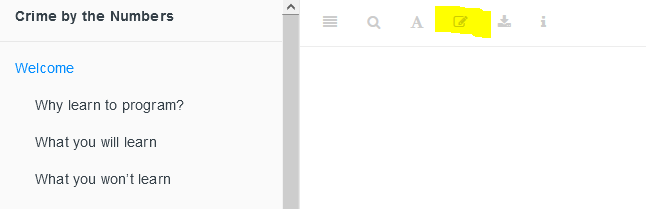
\includegraphics[width=0.9\linewidth]{images/edit_button} 

}

\caption{The edit button for how to make edits of this book.}\label{fig:unnamed-chunk-2}
\end{figure}

\hypertarget{about-the-author-jacob-kaplan}{%
\chapter*{About the author (Jacob Kaplan)}\label{about-the-author-jacob-kaplan}}


\textbf{Jacob Kaplan} holds a PhD and a master's degree in criminology from the University of Pennsylvania and a bachelor's degree in criminal justice from California State University, Sacramento. His research focuses on Crime Prevention Through Environmental Design (CPTED), specifically on the effect of outdoor lighting on crime. He is the author of several R packages that make it easier to work with data, including \href{https://jacobkap.github.io/fastDummies/}{fastDummies} and \href{https://jacobkap.github.io/asciiSetupReader/}{asciiSetupReader}. His \href{http://jacobdkaplan.com/}{website} allows easy analysis of crime-related data and he has released over a \href{http://jacobdkaplan.com/data.html}{dozen crime data sets} (primarily FBI UCR data) on openICPSR that he has compiled, cleaned, and made available to the public.

For a list of papers he has written (including working papers), please see \href{http://jacobdkaplan.com/research.html}{here}.

For a list of data sets he has cleaned, aggregated, and made public, please see \href{http://jacobdkaplan.com/data.html}{here}.

For a list of R packages he has created, please see \href{https://jacobdkaplan.com/packages.html}{here}.

\hypertarget{introduction-to-r-and-rstudio}{%
\chapter{Introduction to R and RStudio}\label{introduction-to-r-and-rstudio}}

\hypertarget{using-rstudio}{%
\section{Using RStudio}\label{using-rstudio}}

In this lesson we'll start by looking at RStudio then write some brief code to load in some crime data and start exploring it. This lesson will cover code that you won't understand completely yet. That is fine, we'll cover everything in more detail as the lessons progress.

RStudio is the interface we use to work with R. It has a number of features to make it easier for us to work with R - while not strictly necessary to use, most people who use R do so through RStudio. We'll spend some time right now looking at RStudio and the options you can change to make it easier to use (and to suit your personal preferences with appearance) as this will make all of the work that we do in this book easier.

When you open up RStudio you'll see four panels, each of which plays an important role in RStudio. Your RStudio may not look like the setup I have in the image below - that is fine, we'll learn how to change the appearance of RStudio soon.

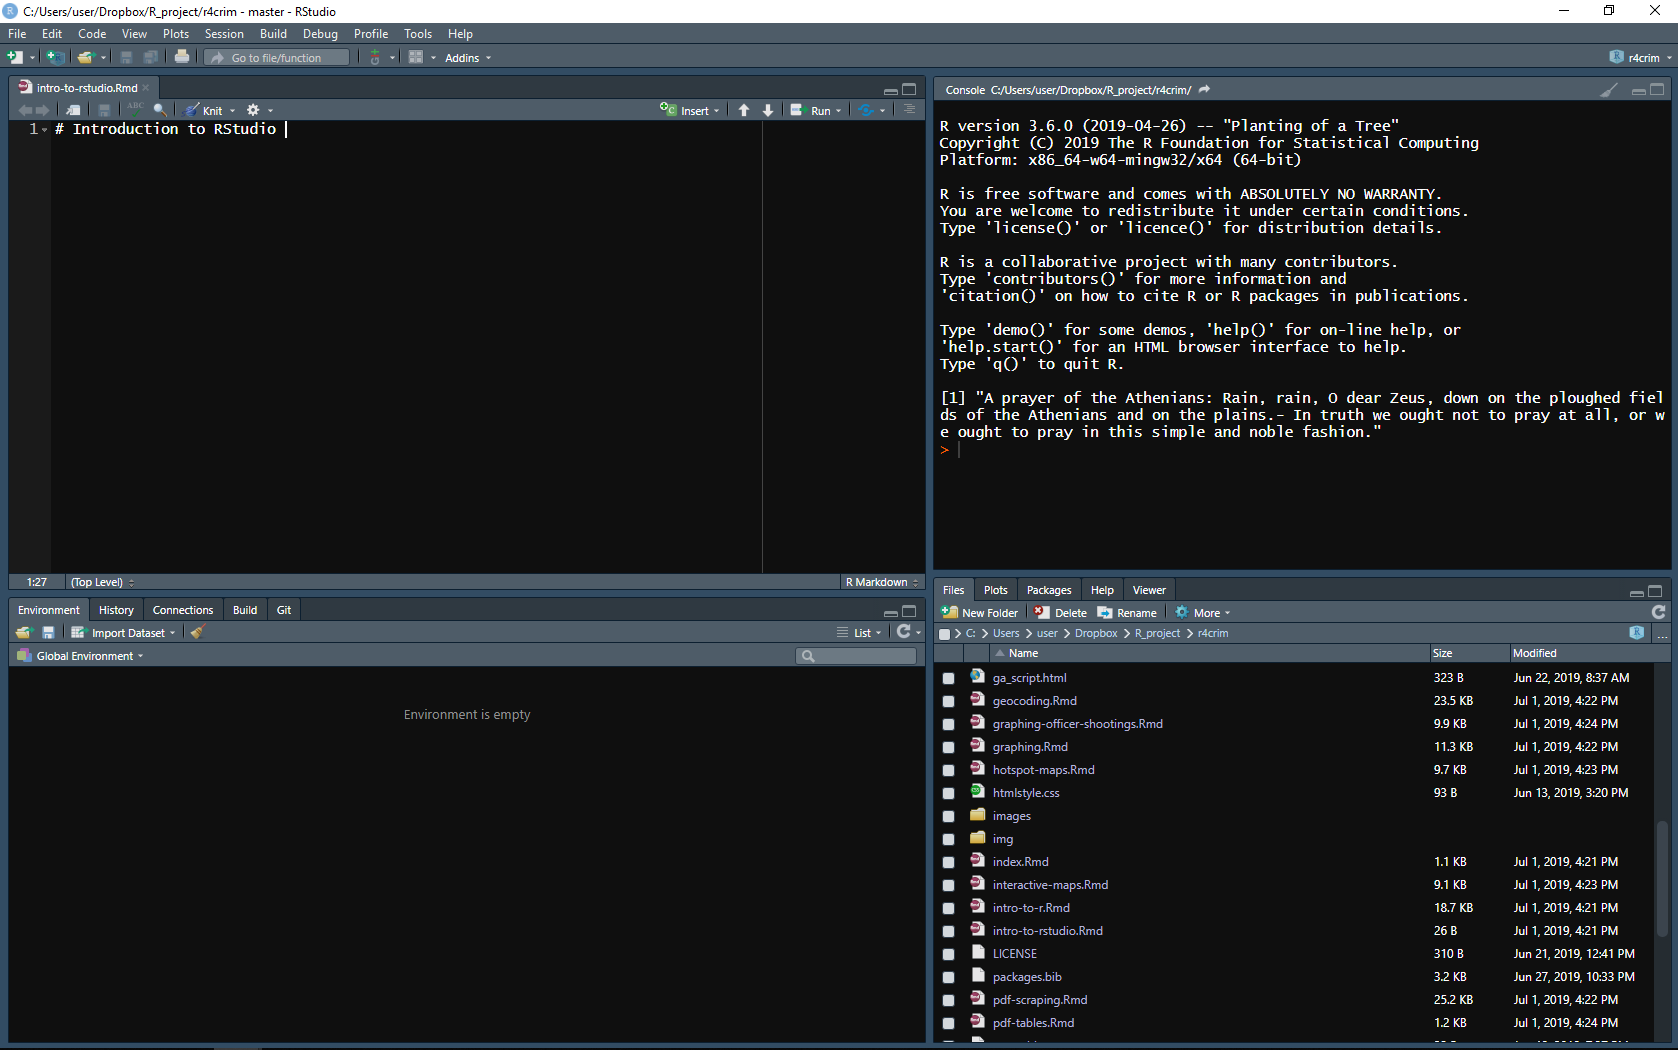
\includegraphics{images/rstudio_1.PNG}

At the top right is the Console panel. Here you can write code, hit enter/return, and R will run that code. If you write \texttt{2+2} it will return (in this case that just mean it will print an answer) 4. This is useful for doing something simple like using R as a calculator or quickly looking at data. In most cases during research this is where you'd do something that you don't care to keep. This is because when you restart R it won't save anything written in the Console. To do reproducible research or to be able to collaborate with others you need a way to keep the code you've written.

The way to keep the code you've written in a file that you can open later or share with someone else is by writing code in an R Script (if you're familiar with Stata, an R Script is just like a .do file). An R Script is essentially a text file (similar to a Word document) where you write code. To run code in an R Script just click on a line of code or highlight several lines and hit enter/return or click the ``Run'' button on the top right of the Source panel. You'll see the lines of code run in the Console and any output (if your code has an output) will be shown there too (making a plot will be shown in a different panel as we'll see soon).

For code that you don't want to run, called comments, start the line with a pound sign \# and that line will not be run (it will still print in the console if you run it but it won't do anything). These comments should explain the code you wrote (if not otherwise obvious).

The Source panel is where the R Scripts will be and is located at the top left on the image below. It is good practice to do all of your code writing in an R Script - even if you delete some lines of code later - as it eliminates the possibility of losing code or forgetting what you wrote. Having all the code in front of you in a text file also makes it easier to understand the flow of code from start to finish to a task - an issue we'll discuss more in later lessons.

While the Source and Console panels are the ones that are of most use, there are two other panels worth discussing. As these two panels let you interchange which tabs are available in them, we'll return to them shortly in the discussion of the options RStudio has to customize it.

\hypertarget{opening-an-r-script}{%
\subsection{Opening an R Script}\label{opening-an-r-script}}

When you want to open up a new R Script you can click File on the very top left, then R Script. It will open up the script in a new tab inside of the Source panel. There are also a number of other file options available: R Presentation which can make PowerPoints, R Markdown which can make Word Documents or PDFs that incorporate R code used to make tables or graphs (and which we'll cover in Chapter \ref{r-markdown}), and Shiny Web App to make websites using R. There is too much to cover for an introductory book such as this but keep in mind the wide capabilities of R if you have another task to do.

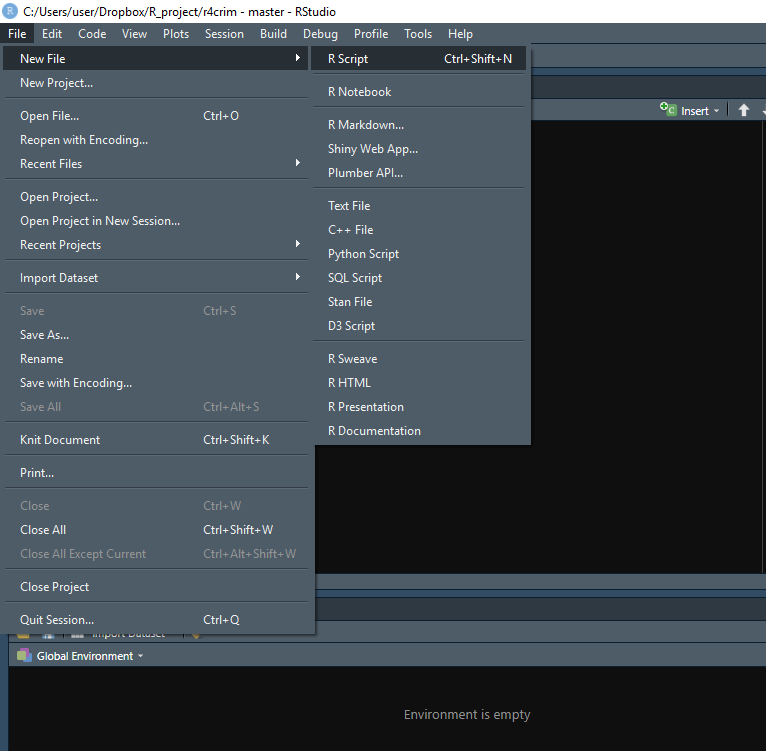
\includegraphics{images/rstudio_2.PNG}

\hypertarget{setting-the-working-directory}{%
\subsection{Setting the working directory}\label{setting-the-working-directory}}

Many research projects incorporate data that someone else (such as the FBI or a local police agency) has put together. In these cases, we need to load the data into R to be able to use it. In a little bit we'll load a data set into R and start working on it but let's take a step back now and think about how to even load data. First, we'll need to get the data onto our computer somehow, probably by downloading it from an agency's website. Let's be specific - we don't download it to our computer, we download it to a specific folder on our computer (usually defaulted to the Downloads folder on a Windows machine). So let's say you wanted to load a file called ``data'' into R. If you have a file called ``data'' in both your Desktop and your Downloads folder, R wouldn't know which one you wanted. And unless your data was in the folder R searches by default (which may not be where the file is downloaded by default), R won't know which file to load.

We need to tell R explicitly which folder has the data to load. We do this by setting the ``Working Directory'' (or the ``Folders where I want you, R, to look for my data'' in more simple terms). To set a working directory in R click the Session tab on the top menu, scroll to Set Working Directory, then click Choose Directory. This will open a window where you can navigate to the folder you want.

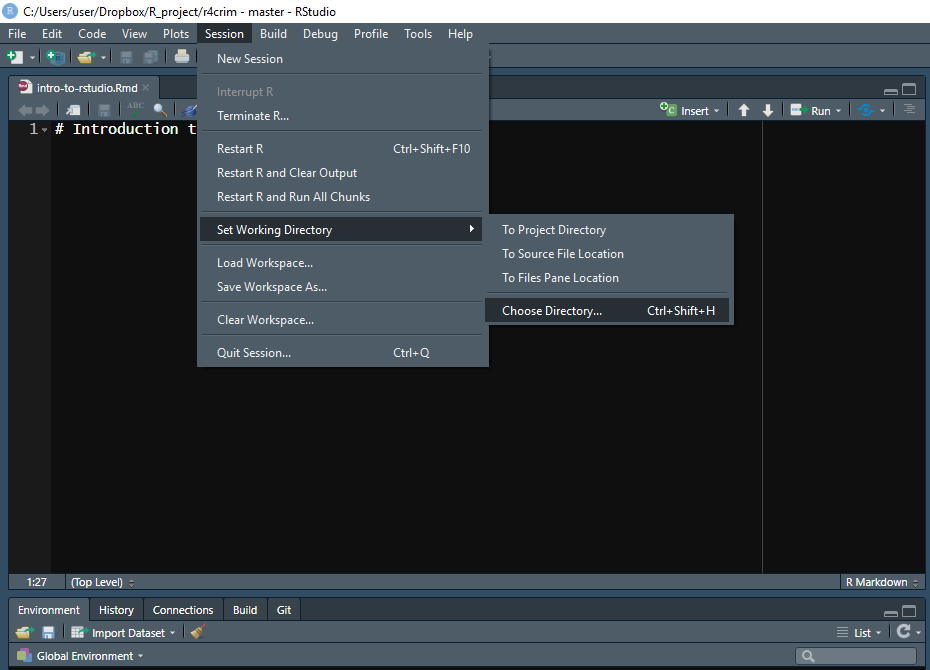
\includegraphics{images/rstudio_3.PNG}

After clicking Open in that window you'll see a new line of code in the Console starting with \texttt{setwd()} and inside of the parentheses is the route your computer takes to get to the folder you selected. And now R knows which folder to look in for the data you want. It is good form to start your R Script with \texttt{setwd()} to make sure you can load the data. Copy the line of code that says \texttt{setwd()} (which stands for ``set working directory''), including everything in the parentheses, to your R Script when you start working.

\hypertarget{changing-rstudio}{%
\subsection{Changing RStudio}\label{changing-rstudio}}

Your RStudio looks different than my RStudio because I changed a number of settings to suit my preferences. To do so yourself click the Tools tab on the top menu and then click Global Options.

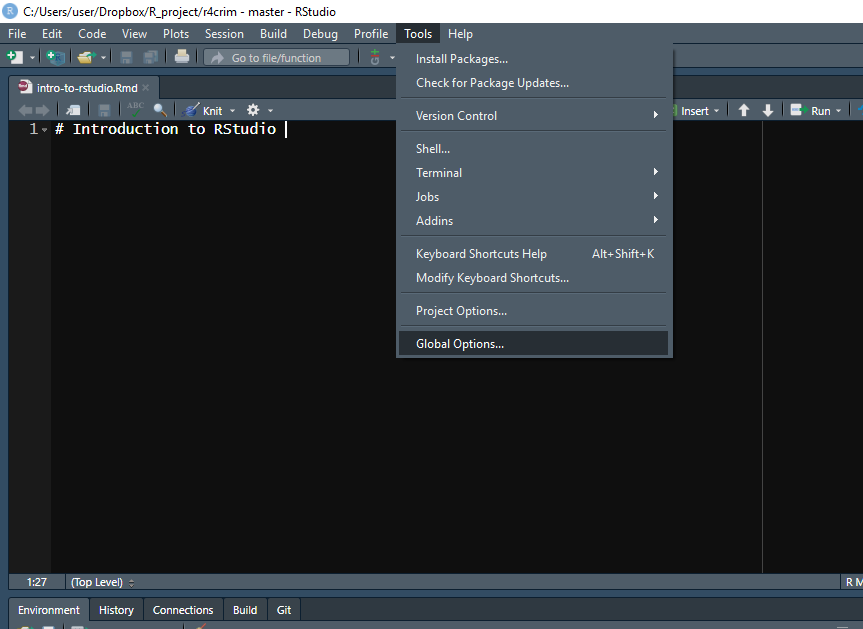
\includegraphics{images/rstudio_5.PNG}

This opens up a window with a number of different tabs to change how R behaves and how it looks.

\hypertarget{general}{%
\subsubsection{General}\label{general}}

Under Workspace in the General tab make sure to \textbf{uncheck} the ``Restore .RData into workspace at startup'' and to set ``Save workspace to .RData on exit:'' to Never. What this does is make sure that every time you open R it starts fresh with no objects (essentially data loaded into R or made in R) from previous sessions. This may be annoying at times, especially when it comes to loading large files, but the benefits far outweigh the costs.

You want your code to run from start to finish without any errors. Something I've seen many students do is write some code in the Console (or in their R Script but out of order of how it should be run) to fix an issue with the data. This means their data is how it should be but when the R session restarts (such as if the computer restarts) they won't be able to get back to that point. Making sure your code handles everything from start to finish is well-worth the avoided headache of trying to remember what code you did to fix the issue previously.

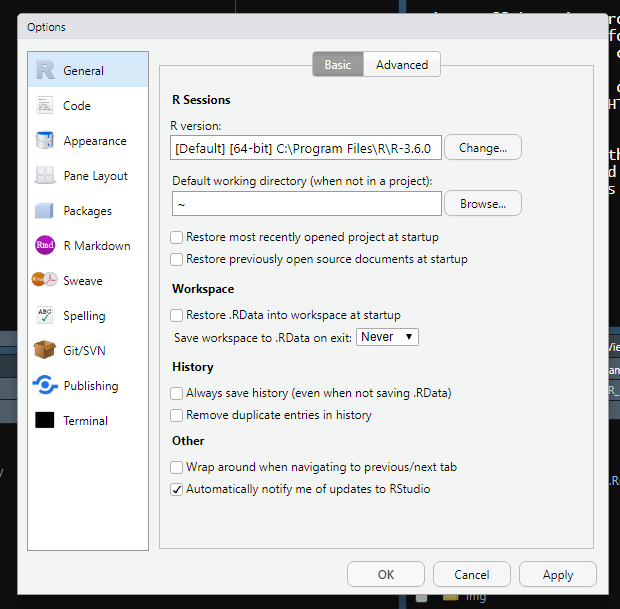
\includegraphics{images/rstudio_6.PNG}

\hypertarget{code}{%
\subsubsection{Code}\label{code}}

The Code tab lets you specify how you want the code to be displayed. The important section for us is to make sure to check the ``Soft-wrap R source files'' check-box. If you write a very long line of code it gets too big to view all at once and you must scroll to the right to read it all. That can be annoying as you won't be able to see all the code at once. Setting ``Soft-wrap'' makes it so if a line is too long it will just be shown on multiple lines which solves that issue. In practice it is best to avoid long lines of codes as it makes it hard to read but that isn't always possible.

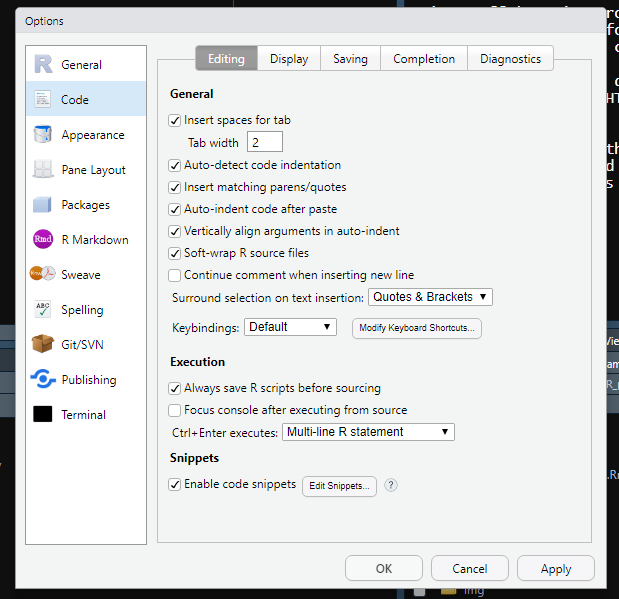
\includegraphics{images/rstudio_7.PNG}

\hypertarget{appearance}{%
\subsubsection{Appearance}\label{appearance}}

The Appearance tab lets you change the background, color, and size of text. Change it to your preferences.

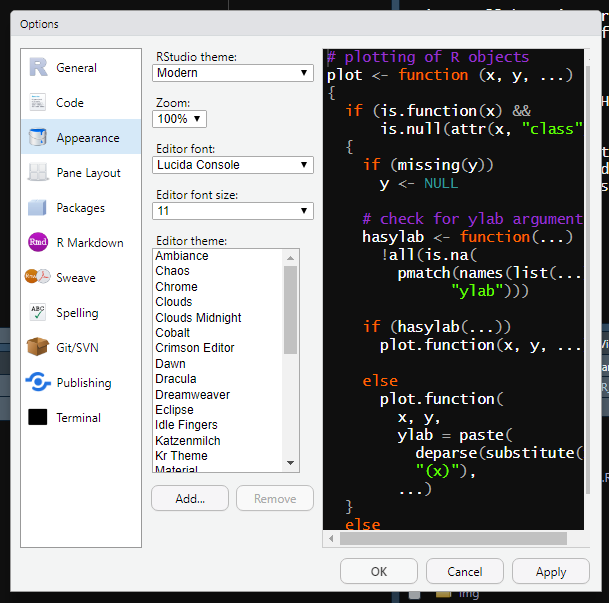
\includegraphics{images/rstudio_8.PNG}

\hypertarget{pane-layout}{%
\subsubsection{Pane Layout}\label{pane-layout}}

The final tab we'll look at is Pane Layout. This lets you move around the Source, Console, and the other two panels. There are a number of different tabs to select for the panels (unchecking one just moves it to the other panel, it doesn't remove it from RStudio) and we'll talk about three of them. The Environment tab shows every object you load into R or make in R. So if you load a file called ``data'' you can check the Environment tab. If it is there, you have loaded the file correctly.

As we'll discuss more in Section \ref{finding-help-about-functions}, the Help tab will open up to show you a help page for a function you want more information on. The Plots tab will display any plot you make. It also keeps all plots you've made (until restarting R) so you can scroll through the plots.

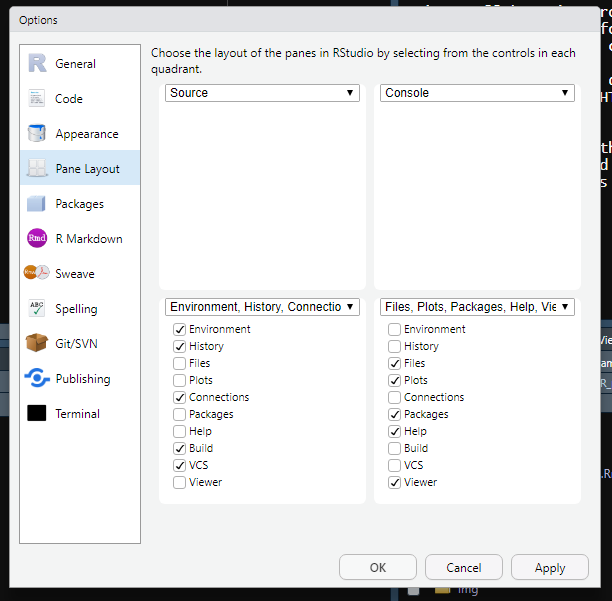
\includegraphics{images/rstudio_9.PNG}

\hypertarget{helpful-cheat-sheets}{%
\subsection{Helpful Cheat Sheets}\label{helpful-cheat-sheets}}

RStudio also includes a number of links to helpful cheat sheets for a few important topics. To get to it click Help, then Cheatsheets and click on whichever one you need.

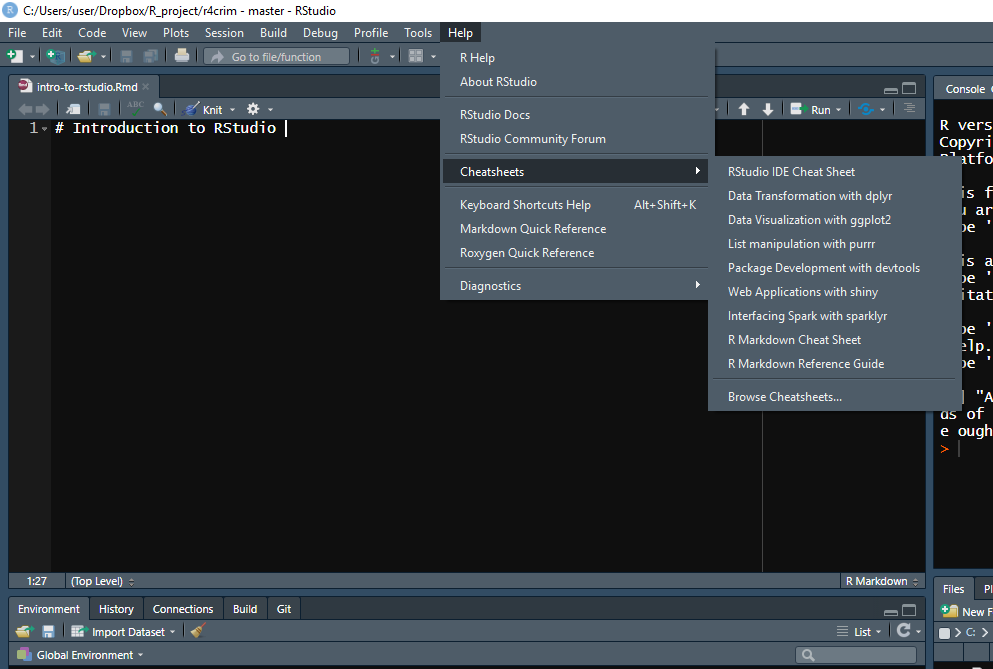
\includegraphics{images/rstudio_4.PNG}

\hypertarget{reading-data-into-r}{%
\section{Reading data into R}\label{reading-data-into-r}}

For many research projects you'll have data produced by some outside group (FBI, local police agencies) and you want to take that data and put it inside R to work on it. We call that reading data into R. R is capable of reading a number of different formats of data which we will discuss in more detail in Chapter \ref{reading-and-writing-data}. Here, we will talk about the standard R data file only.

\hypertarget{loading-data}{%
\subsection{Loading data}\label{loading-data}}

As we learned above in Section \ref{setting-the-working-directory}, we need to set our working directory to the folder where the data is. For my own setup, R is already defaulted to the folder with this data so I do not need to set a working directory. For those following along on your own computer, make sure to set your working directory now.

The \texttt{load()} function lets us load data already in the R format. These files will end in the extension ``.rda'' or sometimes ``.Rda'' or ``.RData''. Since we are telling R to load a specific file, we need to have that file name in quotes and include the file extension ``.rda''. With R data, the object inside the data already has a name so we don't need to assign (something we will discuss in detail in Section \ref{assignment}) a name to the data. With other forms of data such as .csv files we will need to do that as we'll see in Chapter \ref{reading-and-writing-data}.

\begin{Shaded}
\begin{Highlighting}[]
\FunctionTok{load}\NormalTok{(}\StringTok{"data/ucr2017.rda"}\NormalTok{)}
\end{Highlighting}
\end{Shaded}

\hypertarget{first-steps-to-exploring-data}{%
\section{First steps to exploring data}\label{first-steps-to-exploring-data}}

The object we loaded is called \texttt{ucr2017}. We'll explore this data more thoroughly in the Chapter \ref{explore} but for now let's use four simple (and important) functions to get a sense of what the data holds. For each of these functions write the name of the data set (without quotes since we don't need quotes for an object already made in R) inside the ().

\begin{itemize}
\tightlist
\item
  \texttt{head()}
\item
  \texttt{summary()}
\item
  \texttt{plot()}
\item
  \texttt{View()}
\end{itemize}

Note that the first three functions are lowercase while \texttt{View()} is capitalized. That is simply because older functions in R were often capitalized while newer ones use all lowercase letters. R is case sensitive so using \texttt{view()} will not work.

The \texttt{head()} function prints the first 6 rows of each column of the data to the console. This is useful to get a quick glance at the data but has some important drawbacks. When using data with a large number of columns it can be quickly overwhelming by printing too much. There may also be differences in the first 6 rows with other rows. For example, if the rows are ordered chronologically (as is the case with most crime data) the first 6 rows will be the most recent. If data collection methods or the quality of collection changed over time, these 6 rows won't be representative of the data.

\begin{Shaded}
\begin{Highlighting}[]
\FunctionTok{head}\NormalTok{(ucr2017)}
\CommentTok{\#\textgreater{}       ori year agency\_name  state population}
\CommentTok{\#\textgreater{} 1 AK00101 2017   anchorage alaska     296188}
\CommentTok{\#\textgreater{} 2 AK00102 2017   fairbanks alaska      32937}
\CommentTok{\#\textgreater{} 3 AK00103 2017      juneau alaska      32344}
\CommentTok{\#\textgreater{} 4 AK00104 2017   ketchikan alaska       8230}
\CommentTok{\#\textgreater{} 5 AK00105 2017      kodiak alaska       6198}
\CommentTok{\#\textgreater{} 6 AK00106 2017        nome alaska       3829}
\CommentTok{\#\textgreater{}   actual\_murder actual\_rape\_total actual\_robbery\_total}
\CommentTok{\#\textgreater{} 1            27               391                  778}
\CommentTok{\#\textgreater{} 2            10                24                   40}
\CommentTok{\#\textgreater{} 3             1                50                   46}
\CommentTok{\#\textgreater{} 4             1                19                    0}
\CommentTok{\#\textgreater{} 5             0                15                    4}
\CommentTok{\#\textgreater{} 6             0                 7                    0}
\CommentTok{\#\textgreater{}   actual\_assault\_aggravated}
\CommentTok{\#\textgreater{} 1                      2368}
\CommentTok{\#\textgreater{} 2                       131}
\CommentTok{\#\textgreater{} 3                       206}
\CommentTok{\#\textgreater{} 4                        14}
\CommentTok{\#\textgreater{} 5                        41}
\CommentTok{\#\textgreater{} 6                        52}
\end{Highlighting}
\end{Shaded}

The \texttt{summary()} function gives a six number summary of each numeric or Date column in the data. For other types of data, such as ``character'' types (which are just columns with words rather than numbers or dates), it'll say what type of data it is.

The six values it returns for numeric and Date columns are

\begin{itemize}
\tightlist
\item
  The minimum value
\item
  The value at the 1st quartile
\item
  The median value
\item
  The mean value
\item
  The value at the 3rd quartile
\item
  The max value
\item
  In cases where there are NAs, it will say how many NAs there are. An NA value is a missing value. Think of it like an empty cell in an Excel file. NA values will cause issues when doing math such as finding the mean of a column as R doesn't know how to handle a NA value in these situations. We'll learn how to deal with this later.
\end{itemize}

\begin{Shaded}
\begin{Highlighting}[]
\FunctionTok{summary}\NormalTok{(ucr2017)}
\CommentTok{\#\textgreater{}      ori                 year      agency\_name       }
\CommentTok{\#\textgreater{}  Length:15764       Min.   :2017   Length:15764      }
\CommentTok{\#\textgreater{}  Class :character   1st Qu.:2017   Class :character  }
\CommentTok{\#\textgreater{}  Mode  :character   Median :2017   Mode  :character  }
\CommentTok{\#\textgreater{}                     Mean   :2017                     }
\CommentTok{\#\textgreater{}                     3rd Qu.:2017                     }
\CommentTok{\#\textgreater{}                     Max.   :2017                     }
\CommentTok{\#\textgreater{}     state             population      actual\_murder    }
\CommentTok{\#\textgreater{}  Length:15764       Min.   :      0   Min.   :  0.000  }
\CommentTok{\#\textgreater{}  Class :character   1st Qu.:    914   1st Qu.:  0.000  }
\CommentTok{\#\textgreater{}  Mode  :character   Median :   4460   Median :  0.000  }
\CommentTok{\#\textgreater{}                     Mean   :  19872   Mean   :  1.069  }
\CommentTok{\#\textgreater{}                     3rd Qu.:  15390   3rd Qu.:  0.000  }
\CommentTok{\#\textgreater{}                     Max.   :8616333   Max.   :653.000  }
\CommentTok{\#\textgreater{}  actual\_rape\_total  actual\_robbery\_total}
\CommentTok{\#\textgreater{}  Min.   :  {-}2.000   Min.   :   {-}1.00    }
\CommentTok{\#\textgreater{}  1st Qu.:   0.000   1st Qu.:    0.00    }
\CommentTok{\#\textgreater{}  Median :   1.000   Median :    0.00    }
\CommentTok{\#\textgreater{}  Mean   :   8.262   Mean   :   19.85    }
\CommentTok{\#\textgreater{}  3rd Qu.:   5.000   3rd Qu.:    4.00    }
\CommentTok{\#\textgreater{}  Max.   :2455.000   Max.   :13995.00    }
\CommentTok{\#\textgreater{}  actual\_assault\_aggravated}
\CommentTok{\#\textgreater{}  Min.   :   {-}1.00         }
\CommentTok{\#\textgreater{}  1st Qu.:    1.00         }
\CommentTok{\#\textgreater{}  Median :    5.00         }
\CommentTok{\#\textgreater{}  Mean   :   49.98         }
\CommentTok{\#\textgreater{}  3rd Qu.:   21.00         }
\CommentTok{\#\textgreater{}  Max.   :29771.00}
\end{Highlighting}
\end{Shaded}

The \texttt{plot()} function allows us to graph our data. For criminology research we generally want to make scatterplots to show the relationship between two numeric variables, time-series graphs to see how a variable (or variables) change over time, or barplots comparing categorical variables. Here we'll make a scatterplot seeing the relationship between a city's number of murders and their number of aggravated assaults (assault with a weapon or that causes serious bodily injury).

To do so we must specify which column is displayed on the x-axis and which one is displayed on the y-axis. In Section \ref{select-specific-columns} we'll talk explicitly about how to select specific columns from our data. For now, all you need to know is to select a column you write the data set name followed by dollar sign \texttt{\$} followed by the column name. Do not include any quotations or spaces (technically spaces can be included but make it a bit harder to read and are against conventional style when writing R code so we'll exclude them). Inside of \texttt{plot()} we say that ``x = ucr2017\$actual\_murder'' so that column goes on the x-axis and ``y = ucr2017\$actual\_assault\_aggravated'' so aggravated assault goes on the y-axis. And that's all it takes to make a simple graph.

\begin{Shaded}
\begin{Highlighting}[]
\FunctionTok{plot}\NormalTok{(}\AttributeTok{x =}\NormalTok{ ucr2017}\SpecialCharTok{$}\NormalTok{actual\_murder, }\AttributeTok{y =}\NormalTok{ ucr2017}\SpecialCharTok{$}\NormalTok{actual\_assault\_aggravated)}
\end{Highlighting}
\end{Shaded}

\begin{center}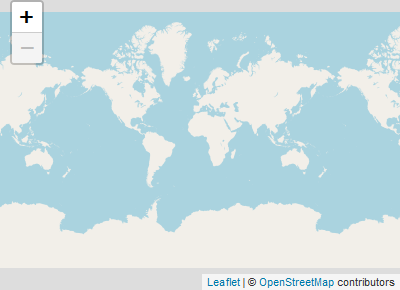
\includegraphics[width=0.9\linewidth]{crimebythenumbers_files/figure-latex/unnamed-chunk-5-1} \end{center}

Finally, \texttt{View()} opens essentially an Excel file of the data set you put inside the (). This allows you to look at the data as if it were in Excel and is a good way to start to understand the data.

\begin{Shaded}
\begin{Highlighting}[]
\FunctionTok{View}\NormalTok{(ucr2017)}
\end{Highlighting}
\end{Shaded}

\hypertarget{finding-help-about-functions}{%
\section{Finding help about functions}\label{finding-help-about-functions}}

If you are having trouble understanding what a function does or how to use it, you can ask R for help and it will open up a page explaining what the function does, what options it has, and examples of how to use it. To do so we write \texttt{help(function)} or \texttt{?function} in the console and it will open up that function's help page.

If we wrote \texttt{help(plot)} to figure out what the \texttt{plot()} function does, it will open up this page. For finding the help page of a function the parentheses (e.g.~\texttt{plot()}) are optional.

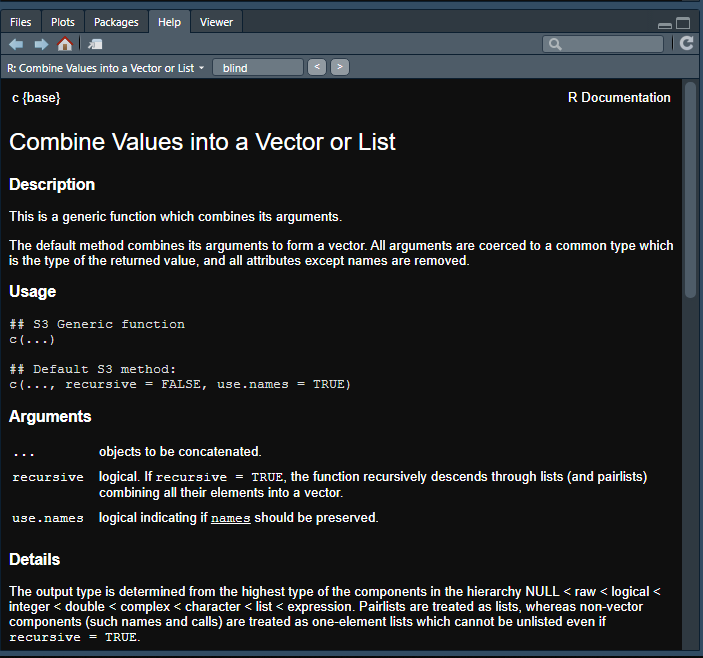
\includegraphics{images/help_page.PNG}

\hypertarget{part-clean}{%
\part{Clean}\label{part-clean}}

\hypertarget{subsetting-intro}{%
\chapter{Subsetting: Making big things small}\label{subsetting-intro}}

Subsetting data is a way to take a large data set and reduce it to a smaller one that is better suited for answering a specific question. This is useful when you have a lot of data in the data set that isn't relevant to your research - for example, if you are studying crime in Colorado and have every state in your data, you'd subset it to keep only the Colorado data. Reducing it to a smaller data set makes it easier to manage, both in understanding your data and avoiding have a huge file that could slow down R.

\hypertarget{select-specific-values}{%
\section{Select specific values}\label{select-specific-values}}

\begin{Shaded}
\begin{Highlighting}[]
\NormalTok{animals }\OtherTok{\textless{}{-}} \FunctionTok{c}\NormalTok{(}\StringTok{"cat"}\NormalTok{, }\StringTok{"dog"}\NormalTok{, }\StringTok{"gorilla"}\NormalTok{, }\StringTok{"buffalo"}\NormalTok{, }\StringTok{"lion"}\NormalTok{, }\StringTok{"snake"}\NormalTok{)}
\end{Highlighting}
\end{Shaded}

\begin{Shaded}
\begin{Highlighting}[]
\NormalTok{animals}
\CommentTok{\#\textgreater{} [1] "cat"     "dog"     "gorilla" "buffalo" "lion"   }
\CommentTok{\#\textgreater{} [6] "snake"}
\end{Highlighting}
\end{Shaded}

Here we have made an object called \emph{animals} with a number of different animals in it (we'll explain what it really means to ``make an object'' soon). In R, we will use square brackets \texttt{{[}{]}} to select specific values in that object, something called ``indexing''. Put a number (or numbers) in the square bracket and it will return the value at that ``index''. The index is just the place number where each value is. ``cat'' is the first value in \emph{animals} so it is at the first index, ``dog'' is the second value so it is the second index or index 2. ``snake'' is our last value and is the 6th value in \emph{animals} so it is index 6 (some languages use ``zero indexing'' which means the first index is index 0, the second is index 1. So in our example ``cat'' would be index 0. R does not do that and the first value is index 1, the second is index 2 and so on.).

The syntax (how the code is written) goes

\texttt{object{[}index{]}}

First, we have the object and then we put the square bracket \texttt{{[}{]}}. We need both the object and the \texttt{{[}{]}} for subsetting to work. Let's say we wanted to choose just the ``snake'' from our \emph{animals} object. In normal language we say "I want the 6th value from \emph{animals}. We say where we're looking and which value we want.

\begin{Shaded}
\begin{Highlighting}[]
\NormalTok{animals[}\DecValTok{6}\NormalTok{]}
\CommentTok{\#\textgreater{} [1] "snake"}
\end{Highlighting}
\end{Shaded}

Now let's get the third value.

\begin{Shaded}
\begin{Highlighting}[]
\NormalTok{animals[}\DecValTok{3}\NormalTok{]}
\CommentTok{\#\textgreater{} [1] "gorilla"}
\end{Highlighting}
\end{Shaded}

If we want multiple values, we can enter multiple numbers. If you have multiple values, you need to make a vector using \texttt{c()} and put the numbers inside the parentheses separated by a comma. We'll learn more about vectors and using \texttt{c()} in Section \ref{vectors} shortly. If we wanted values 1-3, we could use \texttt{c(1,\ 2,\ 3)}, with each number separated by a comma.

\begin{Shaded}
\begin{Highlighting}[]
\NormalTok{animals[}\FunctionTok{c}\NormalTok{(}\DecValTok{1}\NormalTok{, }\DecValTok{2}\NormalTok{, }\DecValTok{3}\NormalTok{)]}
\CommentTok{\#\textgreater{} [1] "cat"     "dog"     "gorilla"}
\end{Highlighting}
\end{Shaded}

When making a vector of sequential integers, instead of writing them all out manually we can use \texttt{first\_number:last\_number} like so

\begin{Shaded}
\begin{Highlighting}[]
\DecValTok{1}\SpecialCharTok{:}\DecValTok{3}
\CommentTok{\#\textgreater{} [1] 1 2 3}
\end{Highlighting}
\end{Shaded}

To use it in subsetting we can treat \texttt{1:3} as if we wrote \texttt{c(1,\ 2,\ 3)}.

\begin{Shaded}
\begin{Highlighting}[]
\NormalTok{animals[}\DecValTok{1}\SpecialCharTok{:}\DecValTok{3}\NormalTok{]}
\CommentTok{\#\textgreater{} [1] "cat"     "dog"     "gorilla"}
\end{Highlighting}
\end{Shaded}

The order we enter the numbers determines the order of the values it returns. Let's get the third index, the fourth index, and the first index, in that order.

\begin{Shaded}
\begin{Highlighting}[]
\NormalTok{animals[}\FunctionTok{c}\NormalTok{(}\DecValTok{3}\NormalTok{, }\DecValTok{4}\NormalTok{, }\DecValTok{1}\NormalTok{)]}
\CommentTok{\#\textgreater{} [1] "gorilla" "buffalo" "cat"}
\end{Highlighting}
\end{Shaded}

Putting a negative number inside the \texttt{{[}{]}} will return all values \textbf{except} for that index, essentially deleting it. Let's remove ``cat'' from \emph{animals}. Since it is the 1st item in \emph{animals}, we can remove it like this

\begin{Shaded}
\begin{Highlighting}[]
\NormalTok{animals[}\SpecialCharTok{{-}}\DecValTok{1}\NormalTok{]}
\CommentTok{\#\textgreater{} [1] "dog"     "gorilla" "buffalo" "lion"    "snake"}
\end{Highlighting}
\end{Shaded}

Now let's remove multiple values, the first 3.

\begin{Shaded}
\begin{Highlighting}[]
\NormalTok{animals[}\SpecialCharTok{{-}}\FunctionTok{c}\NormalTok{(}\DecValTok{1}\NormalTok{, }\DecValTok{2}\NormalTok{, }\DecValTok{3}\NormalTok{)]}
\CommentTok{\#\textgreater{} [1] "buffalo" "lion"    "snake"}
\end{Highlighting}
\end{Shaded}

\hypertarget{assignment}{%
\section{Assigning values to objects (Making ``things'')}\label{assignment}}

Earlier we wrote \texttt{animals\ \textless{}-\ c("cat",\ "dog",\ "gorilla",\ "buffalo",\ "lion",\ "snake")} to make the object \emph{animals} with the value of each of the different animals we wrote.

We say\texttt{\textless{}-} as ``gets''. So above ``animals gets the values cat, dog, etc.''. This is read from left to right as thing on left (the name of the object) ``gets'' the value of the thing on the right of the \texttt{\textless{}-}. The proper terminology is that the ``thing'' on the left is an ``object''. So if we had \texttt{x\ \textless{}-\ 5} the object \emph{x} gets the value 5. We could also say ``five was assigned to x''.

The terminology is ``object gets value'' or ``value assigned to object'', both work.

You can use the \texttt{=} instead of \texttt{\textless{}-}. Again, the thing on the left gets the value of the thing on the right even when using \texttt{=}.

\begin{Shaded}
\begin{Highlighting}[]
\NormalTok{x }\OtherTok{=} \DecValTok{2}
\end{Highlighting}
\end{Shaded}

\emph{x} now has the value of the number 2.

\begin{Shaded}
\begin{Highlighting}[]
\NormalTok{x}
\CommentTok{\#\textgreater{} [1] 2}
\end{Highlighting}
\end{Shaded}

It is the convention in R to use \texttt{\textless{}-} instead of \texttt{=} and in some cases the \texttt{=} will not work properly. For those reasons we will use \texttt{\textless{}-} for this class.

Earlier I said we can remove values with using a negative number and that index will be removed from the object. For example, \texttt{animals{[}-1{]}} prints every value in \emph{animals} except for the first value.

\begin{Shaded}
\begin{Highlighting}[]
\NormalTok{animals[}\SpecialCharTok{{-}}\DecValTok{1}\NormalTok{]}
\CommentTok{\#\textgreater{} [1] "dog"     "gorilla" "buffalo" "lion"    "snake"}
\end{Highlighting}
\end{Shaded}

However, it doesn't actually remove anything from \emph{animals}. Let's print \emph{animals} and see which values it returns.

\begin{Shaded}
\begin{Highlighting}[]
\NormalTok{animals}
\CommentTok{\#\textgreater{} [1] "cat"     "dog"     "gorilla" "buffalo" "lion"   }
\CommentTok{\#\textgreater{} [6] "snake"}
\end{Highlighting}
\end{Shaded}

Now the first value, ``cats'', is back. Why? To make changes in R you need to tell R very explicitly that you are making the change. If you don't save the result of your code (by assigning an object to it), R will run that code and simply print the results in the console panel without making any changes.

This is an important point that a lot of students struggle with. R doesn't know when you want to save (in this context I am referring to creating or updating an object that is entirely in R, not saving a file to your computer) a value or update an object. If \emph{x} is an object with a value of 2, and you write \texttt{x\ +\ 2}, it would print out 4 because 2 + 2 = 4. But that won't change the value of \emph{x}. \emph{x} will remain as 2 until you explicitly tell R to change its value. If you want to update \emph{x} you need to run \texttt{x\ \textless{}-\ somevalue} where ``somevalue'' is whatever you want to change \emph{x} to.

So to return to our \emph{animals} example, if we wanted to delete the first value and keep it removed, we'd need to write \texttt{animals\ \textless{}-\ animals{[}-1{]}}. Which is essentially making a new object, also called \emph{animals} (to avoid having many, slightly different objects that are hard to keep track of we'll reuse the name) with the same values as the original \emph{animals} except this time excluding the first value, ``cats''.

\hypertarget{vectors}{%
\section{Vectors (collections of ``things'')}\label{vectors}}

When we made \emph{x}, we wrote \texttt{x\ \textless{}-\ 2} while when we made \emph{animals}, we wrote \texttt{animals\ \textless{}-\ c("cat",\ "dog",\ "gorilla",\ "buffalo",\ "lion",\ "snake")}. The important difference is that when assigning multiple values to an object we must use the function \texttt{c()} which \textbf{c}ombines them together. With multiple values we follow the same pattern of \texttt{object\ \textless{}-\ value} but put the value inside of \texttt{c()} and separate each value by a comma.

\begin{Shaded}
\begin{Highlighting}[]
\NormalTok{x }\OtherTok{\textless{}{-}} \FunctionTok{c}\NormalTok{(}\DecValTok{1}\NormalTok{, }\DecValTok{2}\NormalTok{, }\DecValTok{3}\NormalTok{)}
\end{Highlighting}
\end{Shaded}

The result of the \texttt{c()} is called a vector and you can think of it as a collection of values.

Note that vectors take values that are the same type, so all values included must be the same type such as a number or a string (a character type such as words or values with letters. In R they are put in quotes.). If they aren't the same type R will automatically convert it.

\begin{Shaded}
\begin{Highlighting}[]
\FunctionTok{c}\NormalTok{(}\StringTok{"cat"}\NormalTok{, }\StringTok{"dog"}\NormalTok{, }\DecValTok{2}\NormalTok{)}
\CommentTok{\#\textgreater{} [1] "cat" "dog" "2"}
\end{Highlighting}
\end{Shaded}

Above we made a vector with the values ``cat'', ``dog'' and 2 (without quotes) and it added quotes to the 2. Since everything must be the same type, R automatically converted the 2 to a string of ``2''.

\hypertarget{logical-values-and-operations}{%
\section{Logical values and operations}\label{logical-values-and-operations}}

We also frequently want to conditionally select certain values. Earlier we selected values indexing specific numbers, but that requires us to know exactly which values we want. We can conditionally select values by having some conditional statement (e.g.~``this value is lower than the number 100'') and keeping only values where that condition is true. When we talk about logical values, we mean TRUE and FALSE - in R you must spell it in all capital letters.

First, we will discuss conditionals abstractly and then we will use a real example using data from the FBI to make a data set tailored to answer a specific question.

We can use these TRUE and FALSE values to index and it will return every element which we say is TRUE.

\begin{Shaded}
\begin{Highlighting}[]
\NormalTok{animals[}\FunctionTok{c}\NormalTok{(}\ConstantTok{TRUE}\NormalTok{, }\ConstantTok{TRUE}\NormalTok{, }\ConstantTok{FALSE}\NormalTok{, }\ConstantTok{FALSE}\NormalTok{, }\ConstantTok{FALSE}\NormalTok{, }\ConstantTok{FALSE}\NormalTok{)]}
\CommentTok{\#\textgreater{} [1] "cat" "dog"}
\end{Highlighting}
\end{Shaded}

This is the basis of conditional subsetting. If we have a large data set and only want a small chunk based on some condition (data in a single state (or multiple states), at a certain time, at least a certain population) we need to make a conditional statement that returns TRUE if it matches what we want and FALSE if it doesn't. There are a number of different ways to make conditional statements. First let's go through some special characters involved and then show examples of each one.

For each case you are asking: does the thing on the left of the conditional statement return TRUE or FALSE compared to the thing on the right.

\begin{itemize}
\tightlist
\item
  \texttt{==} Equals (compared to a single value)
\item
  \texttt{\%in\%} Equals (one value match out of multiple comparisons)
\item
  \texttt{!=} Does not equal
\item
  \texttt{\textless{}} Less than
\item
  \texttt{\textgreater{}} Greater than
\item
  \texttt{\textless{}=} Less than or equal to
\item
  \texttt{\textgreater{}=} Greater than or equal to
\end{itemize}

Since many conditionals involve numbers (especially in criminology), let's make a new object called \emph{numbers} with the numbers 1-10.

\begin{Shaded}
\begin{Highlighting}[]
\NormalTok{numbers }\OtherTok{\textless{}{-}} \DecValTok{1}\SpecialCharTok{:}\DecValTok{10}
\end{Highlighting}
\end{Shaded}

\hypertarget{matching-a-single-value}{%
\subsection{Matching a single value}\label{matching-a-single-value}}

The conditional \texttt{==} asks if the thing on the left equals the thing on the right. Note that it uses two equal signs. If we used only one equal sign it would assign the thing on the left the value of the thing on the right (as if we did \texttt{\textless{}-}).

\begin{Shaded}
\begin{Highlighting}[]
\DecValTok{2} \SpecialCharTok{==} \DecValTok{2}
\CommentTok{\#\textgreater{} [1] TRUE}
\end{Highlighting}
\end{Shaded}

This gives \texttt{TRUE} as we know that 2 does equal 2. If we change either value, it would give us \texttt{FALSE}.

\begin{Shaded}
\begin{Highlighting}[]
\DecValTok{2} \SpecialCharTok{==} \DecValTok{3}
\CommentTok{\#\textgreater{} [1] FALSE}
\end{Highlighting}
\end{Shaded}

And it works when we have multiple numbers on the left side, such as our object called \emph{numbers}.

\begin{Shaded}
\begin{Highlighting}[]
\NormalTok{numbers }\SpecialCharTok{==} \DecValTok{2}
\CommentTok{\#\textgreater{}  [1] FALSE  TRUE FALSE FALSE FALSE FALSE FALSE FALSE}
\CommentTok{\#\textgreater{}  [9] FALSE FALSE}
\end{Highlighting}
\end{Shaded}

This also works with characters such as the animals in the object we made earlier. ``gorilla'' is the third animal in our object, so if we check animals == ``gorilla'' we expect the third value to be \texttt{TRUE} and all others to be \texttt{FALSE}. Make sure that the match is spelled correctly (including capitalization) and is in quotes.

\begin{Shaded}
\begin{Highlighting}[]
\NormalTok{animals }\SpecialCharTok{==} \StringTok{"gorilla"}
\CommentTok{\#\textgreater{} [1] FALSE FALSE  TRUE FALSE FALSE FALSE}
\end{Highlighting}
\end{Shaded}

The \texttt{==} only works when there is one thing on the right hand side. In criminology we often want to know if there is a match for multiple things - is the crime one of the following crimes\ldots, did the crime happen in one of these months\ldots, is the victim a member of these demographic groups\ldots? So we need a way to check if a value is one of many values.

\hypertarget{matching-multiple-values}{%
\subsection{Matching multiple values}\label{matching-multiple-values}}

The R operator \texttt{\%in\%} asks each value on the left whether or not it is a member of the set on the right. It asks, is the single value on the left hand side (even when there are multiple values such as our \emph{animals} object, it goes through them one at a time) a match with any of the values on the right hand side? It only has to match with one of the right hand side values to be a match.

\begin{Shaded}
\begin{Highlighting}[]
\DecValTok{2} \SpecialCharTok{\%in\%} \FunctionTok{c}\NormalTok{(}\DecValTok{1}\NormalTok{, }\DecValTok{2}\NormalTok{, }\DecValTok{3}\NormalTok{) }
\CommentTok{\#\textgreater{} [1] TRUE}
\end{Highlighting}
\end{Shaded}

For our \emph{animals} object, if we check if they are in the vector \texttt{c("cat",\ "dog",\ "gorilla")}, now all three of those animals will return \texttt{TRUE}.

\begin{Shaded}
\begin{Highlighting}[]
\NormalTok{animals }\SpecialCharTok{\%in\%} \FunctionTok{c}\NormalTok{(}\StringTok{"cat"}\NormalTok{, }\StringTok{"dog"}\NormalTok{, }\StringTok{"gorilla"}\NormalTok{)}
\CommentTok{\#\textgreater{} [1]  TRUE  TRUE  TRUE FALSE FALSE FALSE}
\end{Highlighting}
\end{Shaded}

\hypertarget{does-not-match}{%
\subsection{Does not match}\label{does-not-match}}

Sometimes it is easier to ask what is not a match. For example, if you wanted to get every month except January, instead of writing the other 11 months, you just ask for any month that does not equal ``January''.

We can use \texttt{!=}, which means ``not equal''. When we wanted an exact match, we used \texttt{==}, if we want a not match, we can use \texttt{!=} (this time it is only a single equals sign).

\begin{Shaded}
\begin{Highlighting}[]
\DecValTok{2} \SpecialCharTok{!=} \DecValTok{3}
\CommentTok{\#\textgreater{} [1] TRUE}
\end{Highlighting}
\end{Shaded}

\begin{Shaded}
\begin{Highlighting}[]
\StringTok{"cat"} \SpecialCharTok{!=} \StringTok{"gorilla"}
\CommentTok{\#\textgreater{} [1] TRUE}
\end{Highlighting}
\end{Shaded}

Note that for matching multiple values with \texttt{\%in\%}, we cannot write \texttt{!\%in\%} but have to put the \texttt{!} before the values on the left.

\begin{Shaded}
\begin{Highlighting}[]
\SpecialCharTok{!}\NormalTok{animals }\SpecialCharTok{\%in\%} \FunctionTok{c}\NormalTok{(}\StringTok{"cat"}\NormalTok{, }\StringTok{"dog"}\NormalTok{, }\StringTok{"gorilla"}\NormalTok{)}
\CommentTok{\#\textgreater{} [1] FALSE FALSE FALSE  TRUE  TRUE  TRUE}
\end{Highlighting}
\end{Shaded}

\hypertarget{greater-than-or-less-than}{%
\subsection{Greater than or less than}\label{greater-than-or-less-than}}

We can use R to compare values using greater than or less than symbols. We can also express ``greater than or equal to'' or ``less than or equal to.''

\begin{Shaded}
\begin{Highlighting}[]
\DecValTok{6} \SpecialCharTok{\textgreater{}} \DecValTok{5}
\CommentTok{\#\textgreater{} [1] TRUE}
\end{Highlighting}
\end{Shaded}

\begin{Shaded}
\begin{Highlighting}[]
\DecValTok{6} \SpecialCharTok{\textless{}} \DecValTok{5}
\CommentTok{\#\textgreater{} [1] FALSE}
\end{Highlighting}
\end{Shaded}

\begin{Shaded}
\begin{Highlighting}[]
\DecValTok{6} \SpecialCharTok{\textgreater{}=} \DecValTok{5}
\CommentTok{\#\textgreater{} [1] TRUE}
\end{Highlighting}
\end{Shaded}

\begin{Shaded}
\begin{Highlighting}[]
\DecValTok{5} \SpecialCharTok{\textless{}=} \DecValTok{5}
\CommentTok{\#\textgreater{} [1] TRUE}
\end{Highlighting}
\end{Shaded}

When used on our object \emph{numbers} it will return 10 values (since \emph{numbers} is 10 elements long) with a \texttt{TRUE} if the condition is true for the element and \texttt{FALSE} otherwise. Let's run \texttt{numbers\ \textgreater{}\ 3}. We expect the first 3 values to be \texttt{FALSE} as 1, 2, and 3 are not larger than 3.

\begin{Shaded}
\begin{Highlighting}[]
\NormalTok{numbers }\SpecialCharTok{\textgreater{}} \DecValTok{3}
\CommentTok{\#\textgreater{}  [1] FALSE FALSE FALSE  TRUE  TRUE  TRUE  TRUE  TRUE}
\CommentTok{\#\textgreater{}  [9]  TRUE  TRUE}
\end{Highlighting}
\end{Shaded}

\hypertarget{combining-conditional-statements---or-and}{%
\subsection{Combining conditional statements - or, and}\label{combining-conditional-statements---or-and}}

In many cases when you are subsetting you will want to subset based on more than one condition. These ``conditional statements'' can be tricky for new R users since you need to remember both what conditions you need \emph{and} the R code to write it. For a simple introduction to combining conditional statements, we'll first start with the dog food instructions for my new puppy Peanut.


\includegraphics{images/peanut.png}

Here, the instructions indicate how much food to feed your dog each day. Then instructions are broken down into dog age \textbf{and} expected size (in pounds/kilograms) and the intersection of these tells you how much food to feed your dog. Even once you figure out how much to feed the dog, there's another conditional statement to figure out whether you feed them twice a day or three times a day.

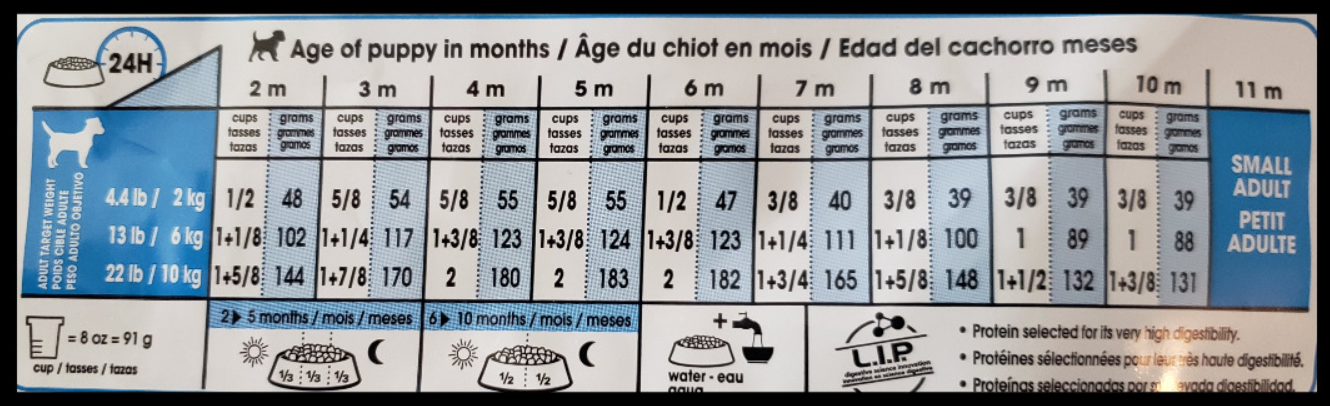
\includegraphics{images/dog_food.PNG}

This food chart is basically a conditional statement matrix where you match the conditions on the left side with those on the right side to figure out how much to feed your dog.\footnote{If you encounter some conditional statements that confuse you - which will be more common and you combine many statements together - I encourage you to make a matrix like this yourself. Even if it isn't that complicated, I think it's easier to see it written down than to try to keep all of the possible conditions in your head.}

So if we wanted to figure out how much to feed a dog that is three months old and will be 4.4 pounds, we'd use the first row on the left (which says 4.4 pounds/2.2 kilograms) and the second columns (which says three months old). When the dog gets to be four months old we'd keep the same row but now move one column to the right. In normal English you'd say that the dog is four months old and their expected size is 4.4 pounds (2 kg). The language when talking about (and writing code for) a conditional statement in programming is a bit more formal where every condition is spoken as a yes or no question. Here we ask is the dog four months old? \textbf{and} is the expected weight 4.4 pounds. If both are true, then we give the dog the amount of food shown for those conditions. If only one is true, then the whole thing is wrong - we wouldn't want to underfeed or overfeed our dog. In this example, a two four old dog can eat between 5/8th of a cup of food and two cups depending on their expected size. So having only one condition be true isn't enough.

Can you see any issue with this conditional statement matrix? It doesn't cover the all possible choices for age and weight combinations. In fact, it is really quite narrow in what it does cover. For example, it covers two and three months, but not any age in between. We can assume that a dog that is 2.5 months old would eat the average of two and three month meal amounts, but wouldn't know for sure. When making your own statements please consider what conditions I am checking for - and, importantly, what I'm leaving out.

For a real data example, let's say you have crime data from every state between 1960 and 2017. Your research question is ``did Colorado's marijuana legalization affect crime in the state?'' In that case you want only data from Colorado. Since legalization began in January 2014, you wouldn't need every year, only years some period of time before and after legalization to be able to measure its effect. So you would need to subset based on the state and the year.

To make conditional statements with multiple conditions we use \texttt{\textbar{}} for ``or'' and \texttt{\&} for ``and''.

\texttt{Condition\ 1\ \textbar{}\ Condition\ 2}

\begin{Shaded}
\begin{Highlighting}[]
\DecValTok{2} \SpecialCharTok{==} \DecValTok{3} \SpecialCharTok{|} \DecValTok{2} \SpecialCharTok{\textgreater{}} \DecValTok{1}
\CommentTok{\#\textgreater{} [1] TRUE}
\end{Highlighting}
\end{Shaded}

As it sounds, when using \texttt{\textbar{}} as long as at least one condition is true (we can include as many conditions as we like) it will return \texttt{TRUE}.

\texttt{Condition\ 1\ \&\ Condition\ 2}

\begin{Shaded}
\begin{Highlighting}[]
\DecValTok{2} \SpecialCharTok{==} \DecValTok{3} \SpecialCharTok{\&} \DecValTok{2} \SpecialCharTok{\textgreater{}} \DecValTok{1}
\CommentTok{\#\textgreater{} [1] FALSE}
\end{Highlighting}
\end{Shaded}

For \texttt{\&}, all of the conditions must be true. If even one condition is not true it will return \texttt{FALSE}.

\hypertarget{subsetting-a-data.frame}{%
\section{Subsetting a data.frame}\label{subsetting-a-data.frame}}

Earlier we were using a simple vector (collection of values). In this class - and in your own work - you will usually work on an entire data set. These generally come in the form called a ``data.frame'' which you can imagine as being like an Excel file with multiple rows and columns.

Let's load in data from the Uniform Crime Report (UCR), an FBI data set that we'll work on in a later lesson. This data has crime data every year from 1960-2017 and for nearly every agency in the country.

\begin{Shaded}
\begin{Highlighting}[]
\FunctionTok{load}\NormalTok{(}\StringTok{"data/offenses\_known\_yearly\_1960\_2017.rda"}\NormalTok{)}
\end{Highlighting}
\end{Shaded}

Let's peak at the first 6 rows and 6 columns using the square bracket notation \texttt{{[}{]}} for data.frames which we'll explain more below.

\begin{Shaded}
\begin{Highlighting}[]
\NormalTok{offenses\_known\_yearly\_1960\_2017[}\DecValTok{1}\SpecialCharTok{:}\DecValTok{6}\NormalTok{, }\DecValTok{1}\SpecialCharTok{:}\DecValTok{6}\NormalTok{]}
\CommentTok{\#\textgreater{}       ori      ori9 agency\_name  state state\_abb year}
\CommentTok{\#\textgreater{} 1 AK00101 AK0010100   anchorage alaska        AK 2017}
\CommentTok{\#\textgreater{} 2 AK00101 AK0010100   anchorage alaska        AK 2016}
\CommentTok{\#\textgreater{} 3 AK00101 AK0010100   anchorage alaska        AK 2015}
\CommentTok{\#\textgreater{} 4 AK00101 AK0010100   anchorage alaska        AK 2014}
\CommentTok{\#\textgreater{} 5 AK00101 AK0010100   anchorage alaska        AK 2013}
\CommentTok{\#\textgreater{} 6 AK00101 AK0010100   anchorage alaska        AK 2012}
\end{Highlighting}
\end{Shaded}

The first 6 rows appear to be agency identification info for Anchorage, Alaska from 2017-2012. For good measure let's check how many rows and columns are in this data. This will give us some guidance on subsetting which we'll see below. \texttt{nrow()} gives us the number of rows and \texttt{ncol()} gives us the number of columns.

\begin{Shaded}
\begin{Highlighting}[]
\FunctionTok{nrow}\NormalTok{(offenses\_known\_yearly\_1960\_2017)}
\CommentTok{\#\textgreater{} [1] 959010}
\end{Highlighting}
\end{Shaded}

\begin{Shaded}
\begin{Highlighting}[]
\FunctionTok{ncol}\NormalTok{(offenses\_known\_yearly\_1960\_2017)}
\CommentTok{\#\textgreater{} [1] 159}
\end{Highlighting}
\end{Shaded}

This is a large file with 159 columns and nearly a million rows. Normally we wouldn't want to print out the names of all 159 columns but let's do this here as we want to know the variables available to subset.

\begin{Shaded}
\begin{Highlighting}[]
\FunctionTok{names}\NormalTok{(offenses\_known\_yearly\_1960\_2017)}
\CommentTok{\#\textgreater{}   [1] "ori"                           }
\CommentTok{\#\textgreater{}   [2] "ori9"                          }
\CommentTok{\#\textgreater{}   [3] "agency\_name"                   }
\CommentTok{\#\textgreater{}   [4] "state"                         }
\CommentTok{\#\textgreater{}   [5] "state\_abb"                     }
\CommentTok{\#\textgreater{}   [6] "year"                          }
\CommentTok{\#\textgreater{}   [7] "number\_of\_months\_reported"     }
\CommentTok{\#\textgreater{}   [8] "fips\_state\_code"               }
\CommentTok{\#\textgreater{}   [9] "fips\_county\_code"              }
\CommentTok{\#\textgreater{}  [10] "fips\_state\_county\_code"        }
\CommentTok{\#\textgreater{}  [11] "fips\_place\_code"               }
\CommentTok{\#\textgreater{}  [12] "fips\_state\_place\_code"         }
\CommentTok{\#\textgreater{}  [13] "agency\_type"                   }
\CommentTok{\#\textgreater{}  [14] "agency\_subtype\_1"              }
\CommentTok{\#\textgreater{}  [15] "agency\_subtype\_2"              }
\CommentTok{\#\textgreater{}  [16] "crosswalk\_agency\_name"         }
\CommentTok{\#\textgreater{}  [17] "census\_name"                   }
\CommentTok{\#\textgreater{}  [18] "population"                    }
\CommentTok{\#\textgreater{}  [19] "population\_group"              }
\CommentTok{\#\textgreater{}  [20] "country\_division"              }
\CommentTok{\#\textgreater{}  [21] "juvenile\_age"                  }
\CommentTok{\#\textgreater{}  [22] "core\_city\_indication"          }
\CommentTok{\#\textgreater{}  [23] "last\_update"                   }
\CommentTok{\#\textgreater{}  [24] "fbi\_field\_office"              }
\CommentTok{\#\textgreater{}  [25] "followup\_indication"           }
\CommentTok{\#\textgreater{}  [26] "zip\_code"                      }
\CommentTok{\#\textgreater{}  [27] "covered\_by\_ori"                }
\CommentTok{\#\textgreater{}  [28] "agency\_count"                  }
\CommentTok{\#\textgreater{}  [29] "date\_of\_last\_update"           }
\CommentTok{\#\textgreater{}  [30] "month\_included\_in"             }
\CommentTok{\#\textgreater{}  [31] "special\_mailing\_group"         }
\CommentTok{\#\textgreater{}  [32] "special\_mailing\_address"       }
\CommentTok{\#\textgreater{}  [33] "first\_line\_of\_mailing\_address" }
\CommentTok{\#\textgreater{}  [34] "second\_line\_of\_mailing\_address"}
\CommentTok{\#\textgreater{}  [35] "third\_line\_of\_mailing\_address" }
\CommentTok{\#\textgreater{}  [36] "fourth\_line\_of\_mailing\_address"}
\CommentTok{\#\textgreater{}  [37] "officers\_killed\_by\_felony"     }
\CommentTok{\#\textgreater{}  [38] "officers\_killed\_by\_accident"   }
\CommentTok{\#\textgreater{}  [39] "officers\_assaulted"            }
\CommentTok{\#\textgreater{}  [40] "actual\_murder"                 }
\CommentTok{\#\textgreater{}  [41] "actual\_manslaughter"           }
\CommentTok{\#\textgreater{}  [42] "actual\_rape\_total"             }
\CommentTok{\#\textgreater{}  [43] "actual\_rape\_by\_force"          }
\CommentTok{\#\textgreater{}  [44] "actual\_rape\_attempted"         }
\CommentTok{\#\textgreater{}  [45] "actual\_robbery\_total"          }
\CommentTok{\#\textgreater{}  [46] "actual\_robbery\_with\_a\_gun"     }
\CommentTok{\#\textgreater{}  [47] "actual\_robbery\_with\_a\_knife"   }
\CommentTok{\#\textgreater{}  [48] "actual\_robbery\_other\_weapon"   }
\CommentTok{\#\textgreater{}  [49] "actual\_robbery\_unarmed"        }
\CommentTok{\#\textgreater{}  [50] "actual\_assault\_total"          }
\CommentTok{\#\textgreater{}  [51] "actual\_assault\_with\_a\_gun"     }
\CommentTok{\#\textgreater{}  [52] "actual\_assault\_with\_a\_knife"   }
\CommentTok{\#\textgreater{}  [53] "actual\_assault\_other\_weapon"   }
\CommentTok{\#\textgreater{}  [54] "actual\_assault\_unarmed"        }
\CommentTok{\#\textgreater{}  [55] "actual\_assault\_simple"         }
\CommentTok{\#\textgreater{}  [56] "actual\_burg\_total"             }
\CommentTok{\#\textgreater{}  [57] "actual\_burg\_force\_entry"       }
\CommentTok{\#\textgreater{}  [58] "actual\_burg\_nonforce\_entry"    }
\CommentTok{\#\textgreater{}  [59] "actual\_burg\_attempted"         }
\CommentTok{\#\textgreater{}  [60] "actual\_theft\_total"            }
\CommentTok{\#\textgreater{}  [61] "actual\_mtr\_veh\_theft\_total"    }
\CommentTok{\#\textgreater{}  [62] "actual\_mtr\_veh\_theft\_car"      }
\CommentTok{\#\textgreater{}  [63] "actual\_mtr\_veh\_theft\_truck"    }
\CommentTok{\#\textgreater{}  [64] "actual\_mtr\_veh\_theft\_other"    }
\CommentTok{\#\textgreater{}  [65] "actual\_all\_crimes"             }
\CommentTok{\#\textgreater{}  [66] "actual\_assault\_aggravated"     }
\CommentTok{\#\textgreater{}  [67] "actual\_index\_violent"          }
\CommentTok{\#\textgreater{}  [68] "actual\_index\_property"         }
\CommentTok{\#\textgreater{}  [69] "actual\_index\_total"            }
\CommentTok{\#\textgreater{}  [70] "tot\_clr\_murder"                }
\CommentTok{\#\textgreater{}  [71] "tot\_clr\_manslaughter"          }
\CommentTok{\#\textgreater{}  [72] "tot\_clr\_rape\_total"            }
\CommentTok{\#\textgreater{}  [73] "tot\_clr\_rape\_by\_force"         }
\CommentTok{\#\textgreater{}  [74] "tot\_clr\_rape\_attempted"        }
\CommentTok{\#\textgreater{}  [75] "tot\_clr\_robbery\_total"         }
\CommentTok{\#\textgreater{}  [76] "tot\_clr\_robbery\_with\_a\_gun"    }
\CommentTok{\#\textgreater{}  [77] "tot\_clr\_robbery\_with\_a\_knife"  }
\CommentTok{\#\textgreater{}  [78] "tot\_clr\_robbery\_other\_weapon"  }
\CommentTok{\#\textgreater{}  [79] "tot\_clr\_robbery\_unarmed"       }
\CommentTok{\#\textgreater{}  [80] "tot\_clr\_assault\_total"         }
\CommentTok{\#\textgreater{}  [81] "tot\_clr\_assault\_with\_a\_gun"    }
\CommentTok{\#\textgreater{}  [82] "tot\_clr\_assault\_with\_a\_knife"  }
\CommentTok{\#\textgreater{}  [83] "tot\_clr\_assault\_other\_weapon"  }
\CommentTok{\#\textgreater{}  [84] "tot\_clr\_assault\_unarmed"       }
\CommentTok{\#\textgreater{}  [85] "tot\_clr\_assault\_simple"        }
\CommentTok{\#\textgreater{}  [86] "tot\_clr\_burg\_total"            }
\CommentTok{\#\textgreater{}  [87] "tot\_clr\_burg\_force\_entry"      }
\CommentTok{\#\textgreater{}  [88] "tot\_clr\_burg\_nonforce\_entry"   }
\CommentTok{\#\textgreater{}  [89] "tot\_clr\_burg\_attempted"        }
\CommentTok{\#\textgreater{}  [90] "tot\_clr\_theft\_total"           }
\CommentTok{\#\textgreater{}  [91] "tot\_clr\_mtr\_veh\_theft\_total"   }
\CommentTok{\#\textgreater{}  [92] "tot\_clr\_mtr\_veh\_theft\_car"     }
\CommentTok{\#\textgreater{}  [93] "tot\_clr\_mtr\_veh\_theft\_truck"   }
\CommentTok{\#\textgreater{}  [94] "tot\_clr\_mtr\_veh\_theft\_other"   }
\CommentTok{\#\textgreater{}  [95] "tot\_clr\_all\_crimes"            }
\CommentTok{\#\textgreater{}  [96] "tot\_clr\_assault\_aggravated"    }
\CommentTok{\#\textgreater{}  [97] "tot\_clr\_index\_violent"         }
\CommentTok{\#\textgreater{}  [98] "tot\_clr\_index\_property"        }
\CommentTok{\#\textgreater{}  [99] "tot\_clr\_index\_total"           }
\CommentTok{\#\textgreater{} [100] "clr\_18\_murder"                 }
\CommentTok{\#\textgreater{} [101] "clr\_18\_manslaughter"           }
\CommentTok{\#\textgreater{} [102] "clr\_18\_rape\_total"             }
\CommentTok{\#\textgreater{} [103] "clr\_18\_rape\_by\_force"          }
\CommentTok{\#\textgreater{} [104] "clr\_18\_rape\_attempted"         }
\CommentTok{\#\textgreater{} [105] "clr\_18\_robbery\_total"          }
\CommentTok{\#\textgreater{} [106] "clr\_18\_robbery\_with\_a\_gun"     }
\CommentTok{\#\textgreater{} [107] "clr\_18\_robbery\_with\_a\_knife"   }
\CommentTok{\#\textgreater{} [108] "clr\_18\_robbery\_other\_weapon"   }
\CommentTok{\#\textgreater{} [109] "clr\_18\_robbery\_unarmed"        }
\CommentTok{\#\textgreater{} [110] "clr\_18\_assault\_total"          }
\CommentTok{\#\textgreater{} [111] "clr\_18\_assault\_with\_a\_gun"     }
\CommentTok{\#\textgreater{} [112] "clr\_18\_assault\_with\_a\_knife"   }
\CommentTok{\#\textgreater{} [113] "clr\_18\_assault\_other\_weapon"   }
\CommentTok{\#\textgreater{} [114] "clr\_18\_assault\_unarmed"        }
\CommentTok{\#\textgreater{} [115] "clr\_18\_assault\_simple"         }
\CommentTok{\#\textgreater{} [116] "clr\_18\_burg\_total"             }
\CommentTok{\#\textgreater{} [117] "clr\_18\_burg\_force\_entry"       }
\CommentTok{\#\textgreater{} [118] "clr\_18\_burg\_nonforce\_entry"    }
\CommentTok{\#\textgreater{} [119] "clr\_18\_burg\_attempted"         }
\CommentTok{\#\textgreater{} [120] "clr\_18\_theft\_total"            }
\CommentTok{\#\textgreater{} [121] "clr\_18\_mtr\_veh\_theft\_total"    }
\CommentTok{\#\textgreater{} [122] "clr\_18\_mtr\_veh\_theft\_car"      }
\CommentTok{\#\textgreater{} [123] "clr\_18\_mtr\_veh\_theft\_truck"    }
\CommentTok{\#\textgreater{} [124] "clr\_18\_mtr\_veh\_theft\_other"    }
\CommentTok{\#\textgreater{} [125] "clr\_18\_all\_crimes"             }
\CommentTok{\#\textgreater{} [126] "clr\_18\_assault\_aggravated"     }
\CommentTok{\#\textgreater{} [127] "clr\_18\_index\_violent"          }
\CommentTok{\#\textgreater{} [128] "clr\_18\_index\_property"         }
\CommentTok{\#\textgreater{} [129] "clr\_18\_index\_total"            }
\CommentTok{\#\textgreater{} [130] "unfound\_murder"                }
\CommentTok{\#\textgreater{} [131] "unfound\_manslaughter"          }
\CommentTok{\#\textgreater{} [132] "unfound\_rape\_total"            }
\CommentTok{\#\textgreater{} [133] "unfound\_rape\_by\_force"         }
\CommentTok{\#\textgreater{} [134] "unfound\_rape\_attempted"        }
\CommentTok{\#\textgreater{} [135] "unfound\_robbery\_total"         }
\CommentTok{\#\textgreater{} [136] "unfound\_robbery\_with\_a\_gun"    }
\CommentTok{\#\textgreater{} [137] "unfound\_robbery\_with\_a\_knife"  }
\CommentTok{\#\textgreater{} [138] "unfound\_robbery\_other\_weapon"  }
\CommentTok{\#\textgreater{} [139] "unfound\_robbery\_unarmed"       }
\CommentTok{\#\textgreater{} [140] "unfound\_assault\_total"         }
\CommentTok{\#\textgreater{} [141] "unfound\_assault\_with\_a\_gun"    }
\CommentTok{\#\textgreater{} [142] "unfound\_assault\_with\_a\_knife"  }
\CommentTok{\#\textgreater{} [143] "unfound\_assault\_other\_weapon"  }
\CommentTok{\#\textgreater{} [144] "unfound\_assault\_unarmed"       }
\CommentTok{\#\textgreater{} [145] "unfound\_assault\_simple"        }
\CommentTok{\#\textgreater{} [146] "unfound\_burg\_total"            }
\CommentTok{\#\textgreater{} [147] "unfound\_burg\_force\_entry"      }
\CommentTok{\#\textgreater{} [148] "unfound\_burg\_nonforce\_entry"   }
\CommentTok{\#\textgreater{} [149] "unfound\_burg\_attempted"        }
\CommentTok{\#\textgreater{} [150] "unfound\_theft\_total"           }
\CommentTok{\#\textgreater{} [151] "unfound\_mtr\_veh\_theft\_total"   }
\CommentTok{\#\textgreater{} [152] "unfound\_mtr\_veh\_theft\_car"     }
\CommentTok{\#\textgreater{} [153] "unfound\_mtr\_veh\_theft\_truck"   }
\CommentTok{\#\textgreater{} [154] "unfound\_mtr\_veh\_theft\_other"   }
\CommentTok{\#\textgreater{} [155] "unfound\_all\_crimes"            }
\CommentTok{\#\textgreater{} [156] "unfound\_assault\_aggravated"    }
\CommentTok{\#\textgreater{} [157] "unfound\_index\_violent"         }
\CommentTok{\#\textgreater{} [158] "unfound\_index\_property"        }
\CommentTok{\#\textgreater{} [159] "unfound\_index\_total"}
\end{Highlighting}
\end{Shaded}

Now let's discuss how to subset this data into a smaller data set to answer a specific question. Let's subset the data to answer our above question of ``did Colorado's marijuana legalization affect crime in the state?'' Like mentioned above, we need data just from Colorado and just for years around the legalization year - we can do 2011-2017 for simplicity.

We also don't need all 159 columns in the current data. Let's say we're only interested in if murder changes. We'd need the column called \emph{actual\_murder}, the \emph{state} column (as a check to make sure we subset only Colorado), the \emph{year} column, the \emph{population} column, the \emph{ori} column, and the \emph{agency\_name} column (a real analysis would likely grab geographic variables too to see if changes depended on location but here we're just using it as an example). The last two columns - \emph{ori} and \emph{agency\_name} - aren't strictly necessary but would be useful if checking if an agency's values are reasonable when checking for outliers, a step we won't do here.

Before explaining how to subset from a data.frame, let's write pseudocode (essentially a description of what we are going to do that is readable to people but isn't real code) for our subset.

We want

\begin{itemize}
\tightlist
\item
  Only rows where the state equals Colorado
\item
  Only rows where the year is 2011-2017
\item
  Only the following columns: \emph{actual\_murder}, \emph{state}, \emph{year}, \emph{population}, \emph{ori}, \emph{agency\_name}
\end{itemize}

\hypertarget{select-specific-columns}{%
\subsection{Select specific columns}\label{select-specific-columns}}

The way to select a specific column in R is called the dollar sign notation.

\texttt{data\$column}

We write the data name followed by a \texttt{\$} and then the column name. Make sure there are no spaces, quotes, or misspellings (or capitalization issues). Just the \texttt{data\$column} exactly as it is spelled. Since we are referring to data already read into R, there should not be any quotes for either the data or the column name.

We can do this for the column \emph{agency\_name} in our UCR data. If we wrote this in the console it would print out every single row in the column. Because this data is large (nearly a million rows), I am going to wrap this in \texttt{head()} so it only displays the first 6 rows of the column rather than printing the entire column.

\begin{Shaded}
\begin{Highlighting}[]
\FunctionTok{head}\NormalTok{(offenses\_known\_yearly\_1960\_2017}\SpecialCharTok{$}\NormalTok{agency\_name)}
\CommentTok{\#\textgreater{} [1] "anchorage" "anchorage" "anchorage" "anchorage"}
\CommentTok{\#\textgreater{} [5] "anchorage" "anchorage"}
\end{Highlighting}
\end{Shaded}

They're all the same name because Anchorage Police reported many times and are in the data set multiple times. Let's look at the column \emph{actual\_murder} which shows the annual number of murders in that agency.

\begin{Shaded}
\begin{Highlighting}[]
\FunctionTok{head}\NormalTok{(offenses\_known\_yearly\_1960\_2017}\SpecialCharTok{$}\NormalTok{actual\_murder)}
\CommentTok{\#\textgreater{} [1] 27 28 26 12 14 15}
\end{Highlighting}
\end{Shaded}

One hint is to write out the data set name in the console and hit the Tab key. Wait a couple of seconds and a popup will appear listing every column in the data set. You can scroll through this and then hit enter to select that column.

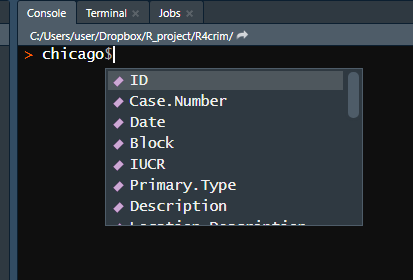
\includegraphics{images/tab_example.png}

\hypertarget{select-specific-rows}{%
\subsection{Select specific rows}\label{select-specific-rows}}

In the earlier examples we used square bracket notation \texttt{{[}{]}} and just put a number or several numbers in the \texttt{{[}{]}}. When dealing with data.frames, however, you need an extra step to tell R which columns to keep. The syntax in the square bracket is

\texttt{{[}row,\ column{]}}

As we did earlier, we start in the square bracket by saying which row we want. Now, since we also have to consider the columns, we need to tell it the number or name (in a vector using \texttt{c()} if more than one name and putting column names in quotes) of the column or columns we want.

The exception to this is when we use the dollar sign notation to select a single column. In that case we don't need a comma (and indeed it will give us an error!). Let's see a few examples and then explain why this works the way it does.

\begin{Shaded}
\begin{Highlighting}[]
\NormalTok{offenses\_known\_yearly\_1960\_2017[}\DecValTok{1}\NormalTok{, }\DecValTok{1}\NormalTok{]}
\CommentTok{\#\textgreater{} [1] "AK00101"}
\end{Highlighting}
\end{Shaded}

If we input multiple numbers, we can get multiple rows and columns.

\begin{Shaded}
\begin{Highlighting}[]
\NormalTok{offenses\_known\_yearly\_1960\_2017[}\DecValTok{1}\SpecialCharTok{:}\DecValTok{6}\NormalTok{, }\DecValTok{1}\SpecialCharTok{:}\DecValTok{6}\NormalTok{]}
\CommentTok{\#\textgreater{}       ori      ori9 agency\_name  state state\_abb year}
\CommentTok{\#\textgreater{} 1 AK00101 AK0010100   anchorage alaska        AK 2017}
\CommentTok{\#\textgreater{} 2 AK00101 AK0010100   anchorage alaska        AK 2016}
\CommentTok{\#\textgreater{} 3 AK00101 AK0010100   anchorage alaska        AK 2015}
\CommentTok{\#\textgreater{} 4 AK00101 AK0010100   anchorage alaska        AK 2014}
\CommentTok{\#\textgreater{} 5 AK00101 AK0010100   anchorage alaska        AK 2013}
\CommentTok{\#\textgreater{} 6 AK00101 AK0010100   anchorage alaska        AK 2012}
\end{Highlighting}
\end{Shaded}

The column section also accepts a vector of the names of the columns. These names must be spelled correctly and in quotes.

\begin{Shaded}
\begin{Highlighting}[]
\NormalTok{offenses\_known\_yearly\_1960\_2017[}\DecValTok{1}\SpecialCharTok{:}\DecValTok{6}\NormalTok{, }\FunctionTok{c}\NormalTok{(}\StringTok{"ori"}\NormalTok{, }\StringTok{"year"}\NormalTok{)]}
\CommentTok{\#\textgreater{}       ori year}
\CommentTok{\#\textgreater{} 1 AK00101 2017}
\CommentTok{\#\textgreater{} 2 AK00101 2016}
\CommentTok{\#\textgreater{} 3 AK00101 2015}
\CommentTok{\#\textgreater{} 4 AK00101 2014}
\CommentTok{\#\textgreater{} 5 AK00101 2013}
\CommentTok{\#\textgreater{} 6 AK00101 2012}
\end{Highlighting}
\end{Shaded}

In cases where we want every row or every column, we just don't put a number. By default, R will return every row/column if you don't specify which ones you want. However, you will still need to include the comma.

Here is every column in the first row.

\begin{Shaded}
\begin{Highlighting}[]
\NormalTok{offenses\_known\_yearly\_1960\_2017[}\DecValTok{1}\NormalTok{, ]}
\CommentTok{\#\textgreater{}       ori      ori9 agency\_name  state state\_abb year}
\CommentTok{\#\textgreater{} 1 AK00101 AK0010100   anchorage alaska        AK 2017}
\CommentTok{\#\textgreater{}   number\_of\_months\_reported fips\_state\_code}
\CommentTok{\#\textgreater{} 1                        12              02}
\CommentTok{\#\textgreater{}   fips\_county\_code fips\_state\_county\_code}
\CommentTok{\#\textgreater{} 1              020                  02020}
\CommentTok{\#\textgreater{}   fips\_place\_code fips\_state\_place\_code}
\CommentTok{\#\textgreater{} 1           03000               0203000}
\CommentTok{\#\textgreater{}               agency\_type agency\_subtype\_1}
\CommentTok{\#\textgreater{} 1 local police department   not applicable}
\CommentTok{\#\textgreater{}   agency\_subtype\_2       crosswalk\_agency\_name}
\CommentTok{\#\textgreater{} 1   not applicable anchorage police department}
\CommentTok{\#\textgreater{}              census\_name population}
\CommentTok{\#\textgreater{} 1 anchorage municipality     296188}
\CommentTok{\#\textgreater{}            population\_group country\_division}
\CommentTok{\#\textgreater{} 1 city 250,000 thru 499,999          pacific}
\CommentTok{\#\textgreater{}   juvenile\_age core\_city\_indication last\_update}
\CommentTok{\#\textgreater{} 1           18     core city of msa       42094}
\CommentTok{\#\textgreater{}   fbi\_field\_office followup\_indication zip\_code}
\CommentTok{\#\textgreater{} 1             3030    send a follow{-}up    99507}
\CommentTok{\#\textgreater{}   covered\_by\_ori agency\_count date\_of\_last\_update}
\CommentTok{\#\textgreater{} 1           \textless{}NA\textgreater{}            1              120717}
\CommentTok{\#\textgreater{}   month\_included\_in}
\CommentTok{\#\textgreater{} 1                 0}
\CommentTok{\#\textgreater{}                                                              special\_mailing\_group}
\CommentTok{\#\textgreater{} 1 the agency is a contributor but not on the mailing list,they are not sent forms.}
\CommentTok{\#\textgreater{}         special\_mailing\_address}
\CommentTok{\#\textgreater{} 1 not a special mailing address}
\CommentTok{\#\textgreater{}   first\_line\_of\_mailing\_address}
\CommentTok{\#\textgreater{} 1               chief of police}
\CommentTok{\#\textgreater{}   second\_line\_of\_mailing\_address}
\CommentTok{\#\textgreater{} 1    anchorage police department}
\CommentTok{\#\textgreater{}   third\_line\_of\_mailing\_address}
\CommentTok{\#\textgreater{} 1                4501 elmore rd}
\CommentTok{\#\textgreater{}   fourth\_line\_of\_mailing\_address}
\CommentTok{\#\textgreater{} 1                  anchorage, ak}
\CommentTok{\#\textgreater{}   officers\_killed\_by\_felony officers\_killed\_by\_accident}
\CommentTok{\#\textgreater{} 1                         0                           0}
\CommentTok{\#\textgreater{}   officers\_assaulted actual\_murder actual\_manslaughter}
\CommentTok{\#\textgreater{} 1                426            27                   3}
\CommentTok{\#\textgreater{}   actual\_rape\_total actual\_rape\_by\_force}
\CommentTok{\#\textgreater{} 1               391                  350}
\CommentTok{\#\textgreater{}   actual\_rape\_attempted actual\_robbery\_total}
\CommentTok{\#\textgreater{} 1                    41                  778}
\CommentTok{\#\textgreater{}   actual\_robbery\_with\_a\_gun actual\_robbery\_with\_a\_knife}
\CommentTok{\#\textgreater{} 1                       249                          69}
\CommentTok{\#\textgreater{}   actual\_robbery\_other\_weapon actual\_robbery\_unarmed}
\CommentTok{\#\textgreater{} 1                         116                    344}
\CommentTok{\#\textgreater{}   actual\_assault\_total actual\_assault\_with\_a\_gun}
\CommentTok{\#\textgreater{} 1                 6448                       621}
\CommentTok{\#\textgreater{}   actual\_assault\_with\_a\_knife}
\CommentTok{\#\textgreater{} 1                         392}
\CommentTok{\#\textgreater{}   actual\_assault\_other\_weapon actual\_assault\_unarmed}
\CommentTok{\#\textgreater{} 1                         704                    651}
\CommentTok{\#\textgreater{}   actual\_assault\_simple actual\_burg\_total}
\CommentTok{\#\textgreater{} 1                  4080              2216}
\CommentTok{\#\textgreater{}   actual\_burg\_force\_entry actual\_burg\_nonforce\_entry}
\CommentTok{\#\textgreater{} 1                    1537                        521}
\CommentTok{\#\textgreater{}   actual\_burg\_attempted actual\_theft\_total}
\CommentTok{\#\textgreater{} 1                   158              10721}
\CommentTok{\#\textgreater{}   actual\_mtr\_veh\_theft\_total actual\_mtr\_veh\_theft\_car}
\CommentTok{\#\textgreater{} 1                       3104                     1934}
\CommentTok{\#\textgreater{}   actual\_mtr\_veh\_theft\_truck actual\_mtr\_veh\_theft\_other}
\CommentTok{\#\textgreater{} 1                        971                        199}
\CommentTok{\#\textgreater{}   actual\_all\_crimes actual\_assault\_aggravated}
\CommentTok{\#\textgreater{} 1             23688                      2368}
\CommentTok{\#\textgreater{}   actual\_index\_violent actual\_index\_property}
\CommentTok{\#\textgreater{} 1                 3564                 16041}
\CommentTok{\#\textgreater{}   actual\_index\_total tot\_clr\_murder}
\CommentTok{\#\textgreater{} 1              19605             28}
\CommentTok{\#\textgreater{}   tot\_clr\_manslaughter tot\_clr\_rape\_total}
\CommentTok{\#\textgreater{} 1                    0                 58}
\CommentTok{\#\textgreater{}   tot\_clr\_rape\_by\_force tot\_clr\_rape\_attempted}
\CommentTok{\#\textgreater{} 1                    48                     10}
\CommentTok{\#\textgreater{}   tot\_clr\_robbery\_total tot\_clr\_robbery\_with\_a\_gun}
\CommentTok{\#\textgreater{} 1                   216                         47}
\CommentTok{\#\textgreater{}   tot\_clr\_robbery\_with\_a\_knife}
\CommentTok{\#\textgreater{} 1                           22}
\CommentTok{\#\textgreater{}   tot\_clr\_robbery\_other\_weapon tot\_clr\_robbery\_unarmed}
\CommentTok{\#\textgreater{} 1                           37                     110}
\CommentTok{\#\textgreater{}   tot\_clr\_assault\_total tot\_clr\_assault\_with\_a\_gun}
\CommentTok{\#\textgreater{} 1                  3576                        249}
\CommentTok{\#\textgreater{}   tot\_clr\_assault\_with\_a\_knife}
\CommentTok{\#\textgreater{} 1                          250}
\CommentTok{\#\textgreater{}   tot\_clr\_assault\_other\_weapon tot\_clr\_assault\_unarmed}
\CommentTok{\#\textgreater{} 1                          413                     436}
\CommentTok{\#\textgreater{}   tot\_clr\_assault\_simple tot\_clr\_burg\_total}
\CommentTok{\#\textgreater{} 1                   2228                250}
\CommentTok{\#\textgreater{}   tot\_clr\_burg\_force\_entry tot\_clr\_burg\_nonforce\_entry}
\CommentTok{\#\textgreater{} 1                      129                         114}
\CommentTok{\#\textgreater{}   tot\_clr\_burg\_attempted tot\_clr\_theft\_total}
\CommentTok{\#\textgreater{} 1                      7                1358}
\CommentTok{\#\textgreater{}   tot\_clr\_mtr\_veh\_theft\_total tot\_clr\_mtr\_veh\_theft\_car}
\CommentTok{\#\textgreater{} 1                         497                       335}
\CommentTok{\#\textgreater{}   tot\_clr\_mtr\_veh\_theft\_truck}
\CommentTok{\#\textgreater{} 1                         145}
\CommentTok{\#\textgreater{}   tot\_clr\_mtr\_veh\_theft\_other tot\_clr\_all\_crimes}
\CommentTok{\#\textgreater{} 1                          17               5983}
\CommentTok{\#\textgreater{}   tot\_clr\_assault\_aggravated tot\_clr\_index\_violent}
\CommentTok{\#\textgreater{} 1                       1348                  1650}
\CommentTok{\#\textgreater{}   tot\_clr\_index\_property tot\_clr\_index\_total}
\CommentTok{\#\textgreater{} 1                   2105                3755}
\CommentTok{\#\textgreater{}   clr\_18\_murder clr\_18\_manslaughter clr\_18\_rape\_total}
\CommentTok{\#\textgreater{} 1             1                   0                 5}
\CommentTok{\#\textgreater{}   clr\_18\_rape\_by\_force clr\_18\_rape\_attempted}
\CommentTok{\#\textgreater{} 1                    4                     1}
\CommentTok{\#\textgreater{}   clr\_18\_robbery\_total clr\_18\_robbery\_with\_a\_gun}
\CommentTok{\#\textgreater{} 1                    9                         1}
\CommentTok{\#\textgreater{}   clr\_18\_robbery\_with\_a\_knife}
\CommentTok{\#\textgreater{} 1                           1}
\CommentTok{\#\textgreater{}   clr\_18\_robbery\_other\_weapon clr\_18\_robbery\_unarmed}
\CommentTok{\#\textgreater{} 1                           0                      7}
\CommentTok{\#\textgreater{}   clr\_18\_assault\_total clr\_18\_assault\_with\_a\_gun}
\CommentTok{\#\textgreater{} 1                  277                        37}
\CommentTok{\#\textgreater{}   clr\_18\_assault\_with\_a\_knife}
\CommentTok{\#\textgreater{} 1                          17}
\CommentTok{\#\textgreater{}   clr\_18\_assault\_other\_weapon clr\_18\_assault\_unarmed}
\CommentTok{\#\textgreater{} 1                          19                     17}
\CommentTok{\#\textgreater{}   clr\_18\_assault\_simple clr\_18\_burg\_total}
\CommentTok{\#\textgreater{} 1                   187                 8}
\CommentTok{\#\textgreater{}   clr\_18\_burg\_force\_entry clr\_18\_burg\_nonforce\_entry}
\CommentTok{\#\textgreater{} 1                       4                          2}
\CommentTok{\#\textgreater{}   clr\_18\_burg\_attempted clr\_18\_theft\_total}
\CommentTok{\#\textgreater{} 1                     2                107}
\CommentTok{\#\textgreater{}   clr\_18\_mtr\_veh\_theft\_total clr\_18\_mtr\_veh\_theft\_car}
\CommentTok{\#\textgreater{} 1                         22                       17}
\CommentTok{\#\textgreater{}   clr\_18\_mtr\_veh\_theft\_truck clr\_18\_mtr\_veh\_theft\_other}
\CommentTok{\#\textgreater{} 1                          2                          3}
\CommentTok{\#\textgreater{}   clr\_18\_all\_crimes clr\_18\_assault\_aggravated}
\CommentTok{\#\textgreater{} 1               429                        90}
\CommentTok{\#\textgreater{}   clr\_18\_index\_violent clr\_18\_index\_property}
\CommentTok{\#\textgreater{} 1                  105                   137}
\CommentTok{\#\textgreater{}   clr\_18\_index\_total unfound\_murder}
\CommentTok{\#\textgreater{} 1                242              5}
\CommentTok{\#\textgreater{}   unfound\_manslaughter unfound\_rape\_total}
\CommentTok{\#\textgreater{} 1                    0                 16}
\CommentTok{\#\textgreater{}   unfound\_rape\_by\_force unfound\_rape\_attempted}
\CommentTok{\#\textgreater{} 1                    16                      0}
\CommentTok{\#\textgreater{}   unfound\_robbery\_total unfound\_robbery\_with\_a\_gun}
\CommentTok{\#\textgreater{} 1                     1                          1}
\CommentTok{\#\textgreater{}   unfound\_robbery\_with\_a\_knife}
\CommentTok{\#\textgreater{} 1                            0}
\CommentTok{\#\textgreater{}   unfound\_robbery\_other\_weapon unfound\_robbery\_unarmed}
\CommentTok{\#\textgreater{} 1                            0                       0}
\CommentTok{\#\textgreater{}   unfound\_assault\_total unfound\_assault\_with\_a\_gun}
\CommentTok{\#\textgreater{} 1                     6                          0}
\CommentTok{\#\textgreater{}   unfound\_assault\_with\_a\_knife}
\CommentTok{\#\textgreater{} 1                            1}
\CommentTok{\#\textgreater{}   unfound\_assault\_other\_weapon unfound\_assault\_unarmed}
\CommentTok{\#\textgreater{} 1                            1                       0}
\CommentTok{\#\textgreater{}   unfound\_assault\_simple unfound\_burg\_total}
\CommentTok{\#\textgreater{} 1                      4                  0}
\CommentTok{\#\textgreater{}   unfound\_burg\_force\_entry unfound\_burg\_nonforce\_entry}
\CommentTok{\#\textgreater{} 1                        0                           0}
\CommentTok{\#\textgreater{}   unfound\_burg\_attempted unfound\_theft\_total}
\CommentTok{\#\textgreater{} 1                      0                  40}
\CommentTok{\#\textgreater{}   unfound\_mtr\_veh\_theft\_total unfound\_mtr\_veh\_theft\_car}
\CommentTok{\#\textgreater{} 1                          70                        53}
\CommentTok{\#\textgreater{}   unfound\_mtr\_veh\_theft\_truck}
\CommentTok{\#\textgreater{} 1                          16}
\CommentTok{\#\textgreater{}   unfound\_mtr\_veh\_theft\_other unfound\_all\_crimes}
\CommentTok{\#\textgreater{} 1                           1                138}
\CommentTok{\#\textgreater{}   unfound\_assault\_aggravated unfound\_index\_violent}
\CommentTok{\#\textgreater{} 1                          2                    24}
\CommentTok{\#\textgreater{}   unfound\_index\_property unfound\_index\_total}
\CommentTok{\#\textgreater{} 1                    110                 134}
\end{Highlighting}
\end{Shaded}

Since there are 159 columns in our data, normally we'd want to avoid printing out all of them. And in most cases, we would save the output of subsets to a new object to be used later rather than just printing the output in the console.

What happens if we forget the comma? If we put in numbers for both rows and columns but don't include a comma between them it will have an error.

\begin{Shaded}
\begin{Highlighting}[]
\NormalTok{offenses\_known\_yearly\_1960\_2017[}\DecValTok{1} \DecValTok{1}\NormalTok{]}
\CommentTok{\#\textgreater{} Error: \textless{}text\textgreater{}:1:35: unexpected numeric constant}
\CommentTok{\#\textgreater{} 1: offenses\_known\_yearly\_1960\_2017[1 1}
\CommentTok{\#\textgreater{}                                       \^{}}
\end{Highlighting}
\end{Shaded}

If we only put in a single number and no comma, it will return the column that matches that number. Here we have number 1 and it will return the first column. We'll wrap it in \texttt{head()} so it doesn't print out a million rows.

\begin{Shaded}
\begin{Highlighting}[]
\FunctionTok{head}\NormalTok{(offenses\_known\_yearly\_1960\_2017[}\DecValTok{1}\NormalTok{])}
\CommentTok{\#\textgreater{}       ori}
\CommentTok{\#\textgreater{} 1 AK00101}
\CommentTok{\#\textgreater{} 2 AK00101}
\CommentTok{\#\textgreater{} 3 AK00101}
\CommentTok{\#\textgreater{} 4 AK00101}
\CommentTok{\#\textgreater{} 5 AK00101}
\CommentTok{\#\textgreater{} 6 AK00101}
\end{Highlighting}
\end{Shaded}

Since R thinks you are requesting a column, and we only have 159 columns in the data, asking for any number above 159 will return an error.

\begin{Shaded}
\begin{Highlighting}[]
\FunctionTok{head}\NormalTok{(offenses\_known\_yearly\_1960\_2017[}\DecValTok{1000}\NormalTok{])}
\CommentTok{\#\textgreater{} Error in \textasciigrave{}[.data.frame\textasciigrave{}(offenses\_known\_yearly\_1960\_2017, 1000): undefined columns selected}
\end{Highlighting}
\end{Shaded}

If you already specify a column using dollar sign notation \texttt{\$}, you do not need to indicate any column in the square brackets\texttt{{[}{]}}. All you need to do is say which row or rows you want.

\begin{Shaded}
\begin{Highlighting}[]
\NormalTok{offenses\_known\_yearly\_1960\_2017}\SpecialCharTok{$}\NormalTok{agency\_name[}\DecValTok{15}\NormalTok{]}
\CommentTok{\#\textgreater{} [1] "anchorage"}
\end{Highlighting}
\end{Shaded}

So make sure when you want a row from a data.frame you always include the comma!

\hypertarget{subset-colorado-data}{%
\subsection{Subset Colorado data}\label{subset-colorado-data}}

Finally we have the tools to subset our UCR data to just be Colorado from 2011-2017. There are three conditional statements we need to make, two for rows and one for columns.

\begin{itemize}
\tightlist
\item
  Only rows where the state equals Colorado
\item
  Only rows where the year is 2011-2017
\item
  Only the following columns: actual\_murder, state, year, population, ori, agency\_name
\end{itemize}

We could use the \texttt{\&} operator to say rows must meet condition 1 and condition 2. Since this is an intro lesson, we will do them as two separate conditional statements. For the first step we want to get all rows in the data where the state equals ``colorado'' (in this data all state names are lowercase). And at this point we want to keep all columns in the data. So let's make a new object called \emph{colorado} to save the result of this subset.

Remember that we want to put the object to the left of the \texttt{{[}{]}} (and touching the \texttt{{[}{]}}) to make sure it returns the data. Just having the conditional statement will only return TRUE or FALSE values. Since we want all columns, we don't need to put anything after the comma (but we must include the comma!).

\begin{Shaded}
\begin{Highlighting}[]
\NormalTok{colorado }\OtherTok{\textless{}{-}}\NormalTok{ offenses\_known\_yearly\_1960\_2017[offenses\_known\_yearly\_1960\_2017}\SpecialCharTok{$}\NormalTok{state }\SpecialCharTok{==} \StringTok{"colorado"}\NormalTok{, ]}
\end{Highlighting}
\end{Shaded}

Now we want to get all the rows where the year is 2011-2017. Since we want to check if the year is one of the years 2011-2017, we will use \texttt{\%in\%} and put the years in a vector \texttt{2011:2017}. This time our primary data set is \emph{colorado}, not \emph{offenses\_known\_yearly\_1960\_2017} since \emph{colorado} has already subsetted to just the state we want. This is how subsetting generally works. You take a large data set, subset it to a smaller one and continue to subset the smaller one to only the data you want.

\begin{Shaded}
\begin{Highlighting}[]
\NormalTok{colorado }\OtherTok{\textless{}{-}}\NormalTok{ colorado[colorado}\SpecialCharTok{$}\NormalTok{year }\SpecialCharTok{\%in\%} \DecValTok{2011}\SpecialCharTok{:}\DecValTok{2017}\NormalTok{, ]}
\end{Highlighting}
\end{Shaded}

Finally we want the columns stated above and to keep every row in the current data. Since the format is \texttt{{[}row,\ column{]}} in this case we keep the ``row'' part blank to indicate that we want every row.

\begin{Shaded}
\begin{Highlighting}[]
\NormalTok{colorado }\OtherTok{\textless{}{-}}\NormalTok{ colorado[ , }\FunctionTok{c}\NormalTok{(}\StringTok{"actual\_murder"}\NormalTok{, }\StringTok{"state"}\NormalTok{, }\StringTok{"year"}\NormalTok{, }\StringTok{"population"}\NormalTok{, }\StringTok{"ori"}\NormalTok{, }\StringTok{"agency\_name"}\NormalTok{)]}
\end{Highlighting}
\end{Shaded}

We can do a quick check using the \texttt{unique()} function. The \texttt{unique()} prints all the unique values in a category, such as a column. We will use it on the \emph{state} and \emph{year} columns to make sure only the values that we want are present.

\begin{Shaded}
\begin{Highlighting}[]
\FunctionTok{unique}\NormalTok{(colorado}\SpecialCharTok{$}\NormalTok{state)}
\CommentTok{\#\textgreater{} [1] "colorado"}
\end{Highlighting}
\end{Shaded}

\begin{Shaded}
\begin{Highlighting}[]
\FunctionTok{unique}\NormalTok{(colorado}\SpecialCharTok{$}\NormalTok{year)}
\CommentTok{\#\textgreater{} [1] 2017 2016 2015 2014 2013 2012 2011}
\end{Highlighting}
\end{Shaded}

The only state is Colorado and the only years are 2011-2017 so our subset worked! This data shows the number of murders in each agency. We want to look at state trends so in Section \ref{aggregate} we will sum up all the murders per year and see if marijuana legalization affected it.

\hypertarget{explore}{%
\chapter{Exploratory data analysis}\label{explore}}

When you first start working on new data it is important to spend some time getting familiar with the data. This includes understanding how many rows and columns it has, what each row means (is each row an offender? a victim? crime in a city over a day/month/year?, etc.), and what columns it has. \textbf{Basically you want to know if the data is capable of answering the question you are asking.}

While not a comprehensive list, the following is a good start for exploratory data analysis of new data sets.

\begin{itemize}
\tightlist
\item
  What are the units (what does each row represent?)?
\item
  What variables are available?
\item
  What time period does it cover?
\item
  Are there outliers? How many?
\item
  Are there missing values? How many?
\end{itemize}

For this lesson we will use a data set of FBI Uniform Crime Reporting (UCR) data for 2017. This data includes every agency that reported their data for all 12 months of the year. Throughout this lesson we will look at some summary statistics for the variables we are interested in and make some basic graphs to visualize the data.

First, we need to load the data. Make sure your working directory is set to the folder where the data is.

\begin{Shaded}
\begin{Highlighting}[]
\FunctionTok{load}\NormalTok{(}\StringTok{"data/ucr2017.rda"}\NormalTok{)}
\end{Highlighting}
\end{Shaded}

As a first step, let's see how many rows and columns are in the data, and glance at the first several rows from each column. \texttt{nrow()} and \texttt{ncol()} tell us the number of rows and columns it has, respectively. Like most functions, what you need to do is put the data set name inside the () (exactly as it is spelled without any quotes).

\begin{Shaded}
\begin{Highlighting}[]
\FunctionTok{nrow}\NormalTok{(ucr2017)}
\CommentTok{\#\textgreater{} [1] 15764}
\end{Highlighting}
\end{Shaded}

\begin{Shaded}
\begin{Highlighting}[]
\FunctionTok{ncol}\NormalTok{(ucr2017)}
\CommentTok{\#\textgreater{} [1] 9}
\end{Highlighting}
\end{Shaded}

The function \texttt{head()} will print out the first 6 rows of every column in the data. Since we only have 9 columns, we will use this function. Be careful when you have many columns (100+) as printing all of them out makes it read to read.

\begin{Shaded}
\begin{Highlighting}[]
\FunctionTok{head}\NormalTok{(ucr2017)}
\CommentTok{\#\textgreater{}       ori year agency\_name  state population}
\CommentTok{\#\textgreater{} 1 AK00101 2017   anchorage alaska     296188}
\CommentTok{\#\textgreater{} 2 AK00102 2017   fairbanks alaska      32937}
\CommentTok{\#\textgreater{} 3 AK00103 2017      juneau alaska      32344}
\CommentTok{\#\textgreater{} 4 AK00104 2017   ketchikan alaska       8230}
\CommentTok{\#\textgreater{} 5 AK00105 2017      kodiak alaska       6198}
\CommentTok{\#\textgreater{} 6 AK00106 2017        nome alaska       3829}
\CommentTok{\#\textgreater{}   actual\_murder actual\_rape\_total actual\_robbery\_total}
\CommentTok{\#\textgreater{} 1            27               391                  778}
\CommentTok{\#\textgreater{} 2            10                24                   40}
\CommentTok{\#\textgreater{} 3             1                50                   46}
\CommentTok{\#\textgreater{} 4             1                19                    0}
\CommentTok{\#\textgreater{} 5             0                15                    4}
\CommentTok{\#\textgreater{} 6             0                 7                    0}
\CommentTok{\#\textgreater{}   actual\_assault\_aggravated}
\CommentTok{\#\textgreater{} 1                      2368}
\CommentTok{\#\textgreater{} 2                       131}
\CommentTok{\#\textgreater{} 3                       206}
\CommentTok{\#\textgreater{} 4                        14}
\CommentTok{\#\textgreater{} 5                        41}
\CommentTok{\#\textgreater{} 6                        52}
\end{Highlighting}
\end{Shaded}

From these results it appears that each row is a single agency's annual data for 2017 and the columns show the number of crimes for four crime categories included (the full UCR data contains many more crimes which we'll see in a later lesson).

Finally, we can run \texttt{names()} to print out every column name. We can already see every name from \texttt{head()} but this is useful when we have many columns and don't want to use \texttt{head()}.

\begin{Shaded}
\begin{Highlighting}[]
\FunctionTok{names}\NormalTok{(ucr2017)}
\CommentTok{\#\textgreater{} [1] "ori"                      }
\CommentTok{\#\textgreater{} [2] "year"                     }
\CommentTok{\#\textgreater{} [3] "agency\_name"              }
\CommentTok{\#\textgreater{} [4] "state"                    }
\CommentTok{\#\textgreater{} [5] "population"               }
\CommentTok{\#\textgreater{} [6] "actual\_murder"            }
\CommentTok{\#\textgreater{} [7] "actual\_rape\_total"        }
\CommentTok{\#\textgreater{} [8] "actual\_robbery\_total"     }
\CommentTok{\#\textgreater{} [9] "actual\_assault\_aggravated"}
\end{Highlighting}
\end{Shaded}

\hypertarget{summary-and-table}{%
\section{Summary and Table}\label{summary-and-table}}

An important function in understanding the data you have is \texttt{summary()} which, as discussed in Section \ref{first-steps-to-exploring-data}, provides summary statistics on the numeric columns you have. Let's take a look at the results before seeing how to do something similar for categorical columns.

\begin{Shaded}
\begin{Highlighting}[]
\FunctionTok{summary}\NormalTok{(ucr2017)}
\CommentTok{\#\textgreater{}      ori                 year      agency\_name       }
\CommentTok{\#\textgreater{}  Length:15764       Min.   :2017   Length:15764      }
\CommentTok{\#\textgreater{}  Class :character   1st Qu.:2017   Class :character  }
\CommentTok{\#\textgreater{}  Mode  :character   Median :2017   Mode  :character  }
\CommentTok{\#\textgreater{}                     Mean   :2017                     }
\CommentTok{\#\textgreater{}                     3rd Qu.:2017                     }
\CommentTok{\#\textgreater{}                     Max.   :2017                     }
\CommentTok{\#\textgreater{}     state             population      actual\_murder    }
\CommentTok{\#\textgreater{}  Length:15764       Min.   :      0   Min.   :  0.000  }
\CommentTok{\#\textgreater{}  Class :character   1st Qu.:    914   1st Qu.:  0.000  }
\CommentTok{\#\textgreater{}  Mode  :character   Median :   4460   Median :  0.000  }
\CommentTok{\#\textgreater{}                     Mean   :  19872   Mean   :  1.069  }
\CommentTok{\#\textgreater{}                     3rd Qu.:  15390   3rd Qu.:  0.000  }
\CommentTok{\#\textgreater{}                     Max.   :8616333   Max.   :653.000  }
\CommentTok{\#\textgreater{}  actual\_rape\_total  actual\_robbery\_total}
\CommentTok{\#\textgreater{}  Min.   :  {-}2.000   Min.   :   {-}1.00    }
\CommentTok{\#\textgreater{}  1st Qu.:   0.000   1st Qu.:    0.00    }
\CommentTok{\#\textgreater{}  Median :   1.000   Median :    0.00    }
\CommentTok{\#\textgreater{}  Mean   :   8.262   Mean   :   19.85    }
\CommentTok{\#\textgreater{}  3rd Qu.:   5.000   3rd Qu.:    4.00    }
\CommentTok{\#\textgreater{}  Max.   :2455.000   Max.   :13995.00    }
\CommentTok{\#\textgreater{}  actual\_assault\_aggravated}
\CommentTok{\#\textgreater{}  Min.   :   {-}1.00         }
\CommentTok{\#\textgreater{}  1st Qu.:    1.00         }
\CommentTok{\#\textgreater{}  Median :    5.00         }
\CommentTok{\#\textgreater{}  Mean   :   49.98         }
\CommentTok{\#\textgreater{}  3rd Qu.:   21.00         }
\CommentTok{\#\textgreater{}  Max.   :29771.00}
\end{Highlighting}
\end{Shaded}

The \texttt{table()} function returns every unique value in a category \textbf{and} how often that value appears. Unlike \texttt{summary()} we can't just put the entire data set into the (), we need to specify a single column. To specify a column you use the dollar sign notation which is \texttt{data\$column}. For most functions we use to examine the data as a whole, you can do the same for a specific column.

\begin{Shaded}
\begin{Highlighting}[]
\FunctionTok{head}\NormalTok{(ucr2017}\SpecialCharTok{$}\NormalTok{agency\_name)}
\CommentTok{\#\textgreater{} [1] "anchorage" "fairbanks" "juneau"    "ketchikan"}
\CommentTok{\#\textgreater{} [5] "kodiak"    "nome"}
\end{Highlighting}
\end{Shaded}

There are only two columns in our data with categorical values that we can use - \emph{year} and \emph{state} so let's use \texttt{table()} on both of them. The columns \emph{ori} and \emph{agency\_name} are also categorical but as each row of data has a unique ORI and name, running \texttt{table()} on those columns would not be helpful.

\begin{Shaded}
\begin{Highlighting}[]
\FunctionTok{table}\NormalTok{(ucr2017}\SpecialCharTok{$}\NormalTok{year)}
\CommentTok{\#\textgreater{} }
\CommentTok{\#\textgreater{}  2017 }
\CommentTok{\#\textgreater{} 15764}
\end{Highlighting}
\end{Shaded}

We can see that every year in our data is 2017, as expected based on the data name. \emph{year} is a numerical column so why can we use \texttt{table()} on it? R doesn't differentiate between numbers and characters when seeing how often each value appears. If we ran \texttt{table()} on the column ``actual\_murder'' it would tell us how many times each unique value in the column appeared in the data. That wouldn't be very useful as we don't really care how many times an agency has 7 murders, for example (though looking for how often a numeric column has the value 0 can be helpful in finding likely erroneous data). As numeric variables often have many more unique values than character variables, it also leads to many values being printed, making it harder to understand. For columns where the number of categories is important to us, such as years, states, neighborhoods, we should use \texttt{table()}.

\begin{Shaded}
\begin{Highlighting}[]
\FunctionTok{table}\NormalTok{(ucr2017}\SpecialCharTok{$}\NormalTok{state)}
\CommentTok{\#\textgreater{} }
\CommentTok{\#\textgreater{}              alabama               alaska }
\CommentTok{\#\textgreater{}                  305                   32 }
\CommentTok{\#\textgreater{}              arizona             arkansas }
\CommentTok{\#\textgreater{}                  107                  273 }
\CommentTok{\#\textgreater{}           california             colorado }
\CommentTok{\#\textgreater{}                  732                  213 }
\CommentTok{\#\textgreater{}          connecticut             delaware }
\CommentTok{\#\textgreater{}                  107                   63 }
\CommentTok{\#\textgreater{} district of columbia              florida }
\CommentTok{\#\textgreater{}                    3                  603 }
\CommentTok{\#\textgreater{}              georgia                 guam }
\CommentTok{\#\textgreater{}                  522                    1 }
\CommentTok{\#\textgreater{}               hawaii                idaho }
\CommentTok{\#\textgreater{}                    4                   95 }
\CommentTok{\#\textgreater{}             illinois              indiana }
\CommentTok{\#\textgreater{}                  696                  247 }
\CommentTok{\#\textgreater{}                 iowa               kansas }
\CommentTok{\#\textgreater{}                  216                  309 }
\CommentTok{\#\textgreater{}             kentucky            louisiana }
\CommentTok{\#\textgreater{}                  352                  192 }
\CommentTok{\#\textgreater{}                maine             maryland }
\CommentTok{\#\textgreater{}                  135                  152 }
\CommentTok{\#\textgreater{}        massachusetts             michigan }
\CommentTok{\#\textgreater{}                  346                  625 }
\CommentTok{\#\textgreater{}            minnesota          mississippi }
\CommentTok{\#\textgreater{}                  397                   71 }
\CommentTok{\#\textgreater{}             missouri              montana }
\CommentTok{\#\textgreater{}                  580                  108 }
\CommentTok{\#\textgreater{}             nebraska               nevada }
\CommentTok{\#\textgreater{}                  225                   59 }
\CommentTok{\#\textgreater{}        new hampshire           new jersey }
\CommentTok{\#\textgreater{}                  176                  576 }
\CommentTok{\#\textgreater{}           new mexico             new york }
\CommentTok{\#\textgreater{}                  116                  532 }
\CommentTok{\#\textgreater{}       north carolina         north dakota }
\CommentTok{\#\textgreater{}                  310                  108 }
\CommentTok{\#\textgreater{}                 ohio             oklahoma }
\CommentTok{\#\textgreater{}                  532                  409 }
\CommentTok{\#\textgreater{}               oregon         pennsylvania }
\CommentTok{\#\textgreater{}                  172                 1473 }
\CommentTok{\#\textgreater{}         rhode island       south carolina }
\CommentTok{\#\textgreater{}                   49                  427 }
\CommentTok{\#\textgreater{}         south dakota            tennessee }
\CommentTok{\#\textgreater{}                   92                  466 }
\CommentTok{\#\textgreater{}                texas                 utah }
\CommentTok{\#\textgreater{}                  999                  125 }
\CommentTok{\#\textgreater{}              vermont             virginia }
\CommentTok{\#\textgreater{}                   85                  407 }
\CommentTok{\#\textgreater{}           washington        west virginia }
\CommentTok{\#\textgreater{}                  250                  200 }
\CommentTok{\#\textgreater{}            wisconsin              wyoming }
\CommentTok{\#\textgreater{}                  433                   57}
\end{Highlighting}
\end{Shaded}

This shows us how many times each state is present in the data. States with a larger population tend to appear more often, this makes sense as those states have more agencies to report. Right now the results are in alphabetical order, but when knowing how frequently something appears, we usually want it ordered by frequency. We can use the \texttt{sort()} function to order the results from \texttt{table()}. Just put the entire \texttt{table()} function inside of the () in \texttt{sort()}.

\begin{Shaded}
\begin{Highlighting}[]
\FunctionTok{sort}\NormalTok{(}\FunctionTok{table}\NormalTok{(ucr2017}\SpecialCharTok{$}\NormalTok{state))}
\CommentTok{\#\textgreater{} }
\CommentTok{\#\textgreater{}                 guam district of columbia }
\CommentTok{\#\textgreater{}                    1                    3 }
\CommentTok{\#\textgreater{}               hawaii               alaska }
\CommentTok{\#\textgreater{}                    4                   32 }
\CommentTok{\#\textgreater{}         rhode island              wyoming }
\CommentTok{\#\textgreater{}                   49                   57 }
\CommentTok{\#\textgreater{}               nevada             delaware }
\CommentTok{\#\textgreater{}                   59                   63 }
\CommentTok{\#\textgreater{}          mississippi              vermont }
\CommentTok{\#\textgreater{}                   71                   85 }
\CommentTok{\#\textgreater{}         south dakota                idaho }
\CommentTok{\#\textgreater{}                   92                   95 }
\CommentTok{\#\textgreater{}              arizona          connecticut }
\CommentTok{\#\textgreater{}                  107                  107 }
\CommentTok{\#\textgreater{}              montana         north dakota }
\CommentTok{\#\textgreater{}                  108                  108 }
\CommentTok{\#\textgreater{}           new mexico                 utah }
\CommentTok{\#\textgreater{}                  116                  125 }
\CommentTok{\#\textgreater{}                maine             maryland }
\CommentTok{\#\textgreater{}                  135                  152 }
\CommentTok{\#\textgreater{}               oregon        new hampshire }
\CommentTok{\#\textgreater{}                  172                  176 }
\CommentTok{\#\textgreater{}            louisiana        west virginia }
\CommentTok{\#\textgreater{}                  192                  200 }
\CommentTok{\#\textgreater{}             colorado                 iowa }
\CommentTok{\#\textgreater{}                  213                  216 }
\CommentTok{\#\textgreater{}             nebraska              indiana }
\CommentTok{\#\textgreater{}                  225                  247 }
\CommentTok{\#\textgreater{}           washington             arkansas }
\CommentTok{\#\textgreater{}                  250                  273 }
\CommentTok{\#\textgreater{}              alabama               kansas }
\CommentTok{\#\textgreater{}                  305                  309 }
\CommentTok{\#\textgreater{}       north carolina        massachusetts }
\CommentTok{\#\textgreater{}                  310                  346 }
\CommentTok{\#\textgreater{}             kentucky            minnesota }
\CommentTok{\#\textgreater{}                  352                  397 }
\CommentTok{\#\textgreater{}             virginia             oklahoma }
\CommentTok{\#\textgreater{}                  407                  409 }
\CommentTok{\#\textgreater{}       south carolina            wisconsin }
\CommentTok{\#\textgreater{}                  427                  433 }
\CommentTok{\#\textgreater{}            tennessee              georgia }
\CommentTok{\#\textgreater{}                  466                  522 }
\CommentTok{\#\textgreater{}             new york                 ohio }
\CommentTok{\#\textgreater{}                  532                  532 }
\CommentTok{\#\textgreater{}           new jersey             missouri }
\CommentTok{\#\textgreater{}                  576                  580 }
\CommentTok{\#\textgreater{}              florida             michigan }
\CommentTok{\#\textgreater{}                  603                  625 }
\CommentTok{\#\textgreater{}             illinois           california }
\CommentTok{\#\textgreater{}                  696                  732 }
\CommentTok{\#\textgreater{}                texas         pennsylvania }
\CommentTok{\#\textgreater{}                  999                 1473}
\end{Highlighting}
\end{Shaded}

And if we want to sort it in decreasing order of frequency, we can use the parameter \texttt{decreasing} in \texttt{sort()} and set it to TRUE. A parameter is just an option used in an R function to change the way the function is used or what output it gives. Almost all functions have these parameters and they are useful if you don't want to use the default setting in the function. This parameter, \texttt{decreasing} changes the \texttt{sort()} output to print from largest to smallest. By default this parameter is set to FALSE and here we say it is equal to TRUE.

\begin{Shaded}
\begin{Highlighting}[]
\FunctionTok{sort}\NormalTok{(}\FunctionTok{table}\NormalTok{(ucr2017}\SpecialCharTok{$}\NormalTok{state), }\AttributeTok{decreasing =} \ConstantTok{TRUE}\NormalTok{)}
\CommentTok{\#\textgreater{} }
\CommentTok{\#\textgreater{}         pennsylvania                texas }
\CommentTok{\#\textgreater{}                 1473                  999 }
\CommentTok{\#\textgreater{}           california             illinois }
\CommentTok{\#\textgreater{}                  732                  696 }
\CommentTok{\#\textgreater{}             michigan              florida }
\CommentTok{\#\textgreater{}                  625                  603 }
\CommentTok{\#\textgreater{}             missouri           new jersey }
\CommentTok{\#\textgreater{}                  580                  576 }
\CommentTok{\#\textgreater{}             new york                 ohio }
\CommentTok{\#\textgreater{}                  532                  532 }
\CommentTok{\#\textgreater{}              georgia            tennessee }
\CommentTok{\#\textgreater{}                  522                  466 }
\CommentTok{\#\textgreater{}            wisconsin       south carolina }
\CommentTok{\#\textgreater{}                  433                  427 }
\CommentTok{\#\textgreater{}             oklahoma             virginia }
\CommentTok{\#\textgreater{}                  409                  407 }
\CommentTok{\#\textgreater{}            minnesota             kentucky }
\CommentTok{\#\textgreater{}                  397                  352 }
\CommentTok{\#\textgreater{}        massachusetts       north carolina }
\CommentTok{\#\textgreater{}                  346                  310 }
\CommentTok{\#\textgreater{}               kansas              alabama }
\CommentTok{\#\textgreater{}                  309                  305 }
\CommentTok{\#\textgreater{}             arkansas           washington }
\CommentTok{\#\textgreater{}                  273                  250 }
\CommentTok{\#\textgreater{}              indiana             nebraska }
\CommentTok{\#\textgreater{}                  247                  225 }
\CommentTok{\#\textgreater{}                 iowa             colorado }
\CommentTok{\#\textgreater{}                  216                  213 }
\CommentTok{\#\textgreater{}        west virginia            louisiana }
\CommentTok{\#\textgreater{}                  200                  192 }
\CommentTok{\#\textgreater{}        new hampshire               oregon }
\CommentTok{\#\textgreater{}                  176                  172 }
\CommentTok{\#\textgreater{}             maryland                maine }
\CommentTok{\#\textgreater{}                  152                  135 }
\CommentTok{\#\textgreater{}                 utah           new mexico }
\CommentTok{\#\textgreater{}                  125                  116 }
\CommentTok{\#\textgreater{}              montana         north dakota }
\CommentTok{\#\textgreater{}                  108                  108 }
\CommentTok{\#\textgreater{}              arizona          connecticut }
\CommentTok{\#\textgreater{}                  107                  107 }
\CommentTok{\#\textgreater{}                idaho         south dakota }
\CommentTok{\#\textgreater{}                   95                   92 }
\CommentTok{\#\textgreater{}              vermont          mississippi }
\CommentTok{\#\textgreater{}                   85                   71 }
\CommentTok{\#\textgreater{}             delaware               nevada }
\CommentTok{\#\textgreater{}                   63                   59 }
\CommentTok{\#\textgreater{}              wyoming         rhode island }
\CommentTok{\#\textgreater{}                   57                   49 }
\CommentTok{\#\textgreater{}               alaska               hawaii }
\CommentTok{\#\textgreater{}                   32                    4 }
\CommentTok{\#\textgreater{} district of columbia                 guam }
\CommentTok{\#\textgreater{}                    3                    1}
\end{Highlighting}
\end{Shaded}

\hypertarget{graphing}{%
\section{Graphing}\label{graphing}}

We often want to make quick plots of our data to get a visual understanding of the data. We will learn a more different way to make graphs in Chapter \ref{graphing-intro} but for now let's use the function \texttt{plot()}.

Let's make a few scatterplots showing the relationship between two variables. With \texttt{plot()} the syntax (how you write the code) is \texttt{plot(x\_axis\_variable,\ y\_axis\_variable)}. So all we need to do is give it the variable for the x- and y-axis. Each dot will represent a single agency (a single row in our data).

\begin{Shaded}
\begin{Highlighting}[]
\FunctionTok{plot}\NormalTok{(ucr2017}\SpecialCharTok{$}\NormalTok{actual\_murder, ucr2017}\SpecialCharTok{$}\NormalTok{actual\_robbery\_total)}
\end{Highlighting}
\end{Shaded}

\begin{center}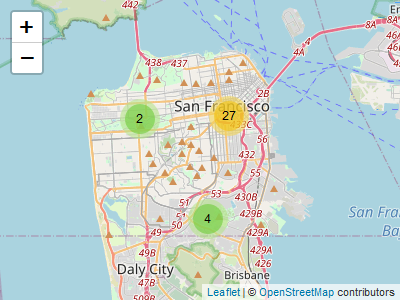
\includegraphics[width=0.9\linewidth]{crimebythenumbers_files/figure-latex/unnamed-chunk-13-1} \end{center}

Above we are telling R to plot the number of murders on the x-axis and the number of robberies on the y-axis. This shows the relationship between a city's number of murders and number of robberies. We can see that there is a relationship where more murders is correlated with more robberies. However, there are a huge number of agencies in the bottom-left corner which have very few murders or robberies. This makes sense as - as we see in the \texttt{summary()} above - most agencies are small, with the median population under 5,000 people.

To try to avoid that clump of small agencies at the bottom, let's make a new data set of only agencies with a population over 1 million. We will use the square bracket \texttt{{[}{]}} notation to subset. Remember it is

\texttt{{[}rows,\ columns{]}}

where we either say exactly which rows or columns we want or give a conditional statement and it'll return only those that meet the condition. We will use the condition that we only want rows where the population is over 1 million.

\texttt{{[}ucr2017\$population\ \textgreater{}\ 1000000,\ {]}}

Now our row conditional is done. We want all the columns in the data so leave the section after the comma empty (don't forget to include that comma!). Now our square bracket notation is done but we need to put it directly to the right of our data so that we take the rows from the right data set.

\texttt{ucr2017{[}ucr2017\$population\ \textgreater{}\ 1000000,\ {]}}

And let's save the results in a new object called ``ucr2017\_big\_cities''.

\begin{Shaded}
\begin{Highlighting}[]
\NormalTok{ucr2017\_big\_cities }\OtherTok{\textless{}{-}}\NormalTok{ ucr2017[ucr2017}\SpecialCharTok{$}\NormalTok{population }\SpecialCharTok{\textgreater{}} \DecValTok{1000000}\NormalTok{, ]}
\end{Highlighting}
\end{Shaded}

Now we can do the same graph as above but using this new data set.

\begin{Shaded}
\begin{Highlighting}[]
\FunctionTok{plot}\NormalTok{(ucr2017\_big\_cities}\SpecialCharTok{$}\NormalTok{actual\_murder, ucr2017\_big\_cities}\SpecialCharTok{$}\NormalTok{actual\_robbery\_total)}
\end{Highlighting}
\end{Shaded}

\begin{center}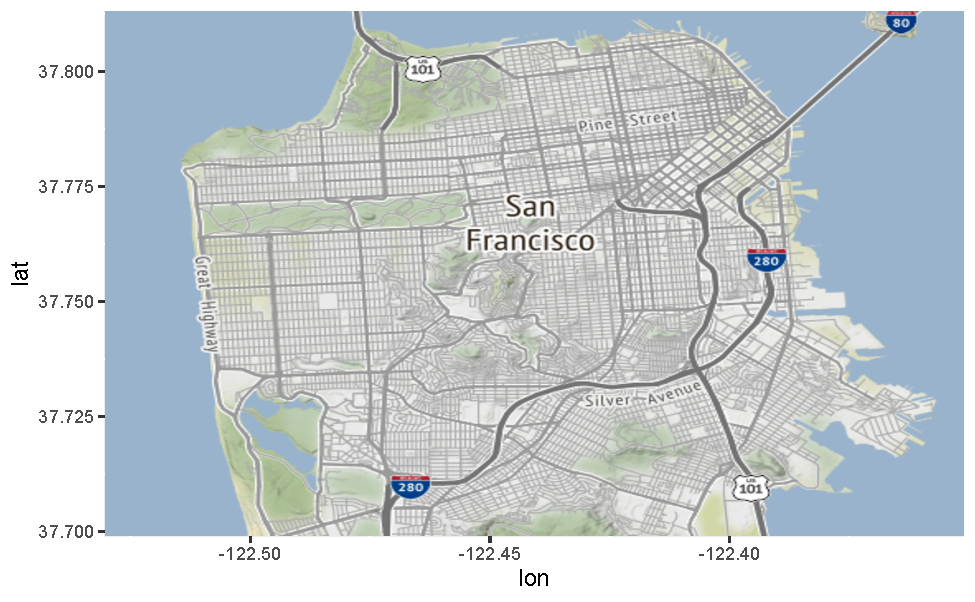
\includegraphics[width=0.9\linewidth]{crimebythenumbers_files/figure-latex/unnamed-chunk-15-1} \end{center}

The problem is somewhat solved. There is still a small clumping of agencies with few robberies or aggravated assaults but the issue is much better. And interestingly the trend is similar with this small subset of data as with all agencies included.

To make our graph look better, we can add labels for the axes and a title (there are many options for changing the appears of this graph, we will just use these three).

\begin{itemize}
\tightlist
\item
  xlab - X-axis label
\item
  ylab - Y-axis label
\item
  main - Graph title
\end{itemize}

Like all parameters, we add them in the () of \texttt{plot()} and separate each parameter by a comma. Since we are adding text to write in the plot, all of these parameter inputs must be in quotes.

\begin{Shaded}
\begin{Highlighting}[]
\FunctionTok{plot}\NormalTok{(ucr2017\_big\_cities}\SpecialCharTok{$}\NormalTok{actual\_murder, ucr2017\_big\_cities}\SpecialCharTok{$}\NormalTok{actual\_robbery\_total,}
     \AttributeTok{xlab =} \StringTok{"Murder"}\NormalTok{,}
     \AttributeTok{ylab =} \StringTok{"Robberies"}\NormalTok{,}
     \AttributeTok{main =} \StringTok{"Relationship between murder and robbery"}\NormalTok{)}
\end{Highlighting}
\end{Shaded}

\begin{center}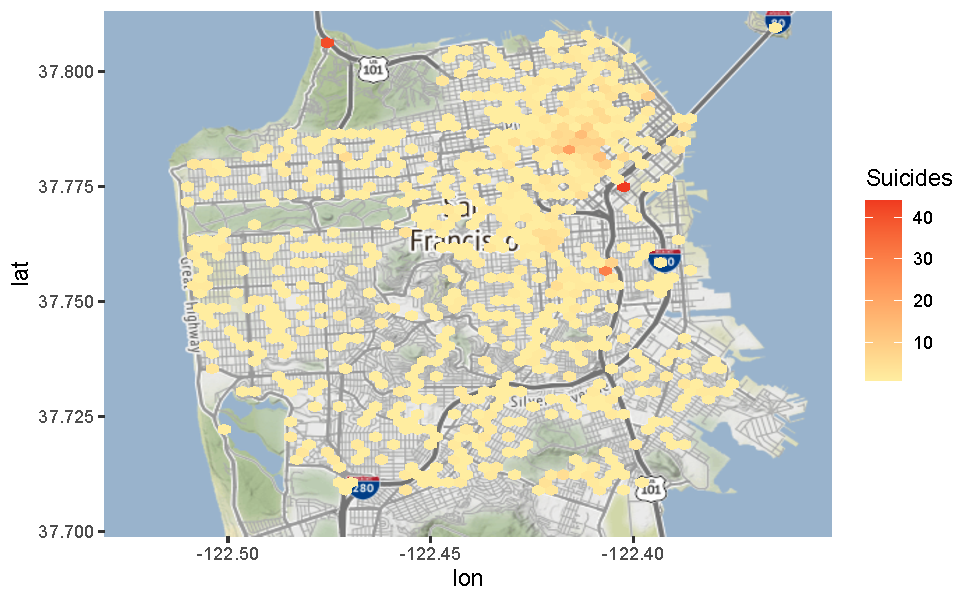
\includegraphics[width=0.9\linewidth]{crimebythenumbers_files/figure-latex/unnamed-chunk-16-1} \end{center}

\hypertarget{aggregate}{%
\section{Aggregating (summaries of groups)}\label{aggregate}}

Right now we have the number of crimes in each agency. For many policy analyses we'd be looking at the effect on the state as a whole, rather than at the agency-level. If we wanted to do this in our data, we would need to \textbf{aggregate} up to the state level. What the \texttt{aggregate()} function does is group values at some higher level than they currently are (e.g.~from agency to state, from day to month, from city street to city neighborhood) and then do some mathematical operation of our choosing (in our case usually sum) to that group.

In Section \ref{subset-colorado-data} we started to see if marijuana legalization affected murder in Colorado. We subsetted the data to only include agencies in Colorado from 2011-2017. Now we can continue to answer the question by aggregating to the state-level to see the total number of murders per year.

Let's think about how our data are and how we would (theoretically, before we write any code) find that out.

Our data is a single row for each agency and we have a column indicating the year the agency reported. So how would be find out how many murders happened in Colorado for each year? Well, first we take all the agencies in 2011 (the first year available) and add up the murders for all agencies that reported that year. Then take all the rows in 2012 and add up their murders. And so on for all the years. That is essentially what \texttt{aggregate()} does. It takes each row and groups them according to the category we specify and then adds up (or does the mathematical operator we specify) each value in each group.

The syntax (how we write the code) is as follows

\texttt{aggregate(numerical\_column\ \textasciitilde{}\ category\_column,\ FUN\ =\ math,\ data\ =\ data\_set)}

The numerical column is the column that we are doing the mathematical operation (sum, mean, median) on. The category column is the one we are using to group (e.g.~state, year). Note the \textasciitilde{} between the numerical and category columns. Unlike most functions where we specify a column name, in \texttt{aggregate()} we do \textbf{not} use quotes for the columns.

FUN is the parameter where we tell \texttt{aggregate()} which mathematical operator to use. Note that FUN is all in capital letters. That is just how this function calls the parameter so we need to make sure we write it in capital letters. data\_set is the name of the data set we are aggregating.

In Chapter \ref{subsetting-intro} we wanted to see if marijuana legalization in Colorado affected murder. To do this we need to have data showing the number of murders for a few years before and after legalization. We have subsetted UCR data to get all agencies in Colorado for the 3 years before and after 2014, the year of legalization. Let's reload that data and rerun the subsetting code.

\begin{Shaded}
\begin{Highlighting}[]
\FunctionTok{load}\NormalTok{(}\StringTok{"data/offenses\_known\_yearly\_1960\_2017.rda"}\NormalTok{)}
\NormalTok{colorado }\OtherTok{\textless{}{-}}\NormalTok{ offenses\_known\_yearly\_1960\_2017[offenses\_known\_yearly\_1960\_2017}\SpecialCharTok{$}\NormalTok{state }\SpecialCharTok{==} \StringTok{"colorado"}\NormalTok{, ]}
\NormalTok{colorado }\OtherTok{\textless{}{-}}\NormalTok{ colorado[colorado}\SpecialCharTok{$}\NormalTok{year }\SpecialCharTok{\%in\%} \DecValTok{2011}\SpecialCharTok{:}\DecValTok{2017}\NormalTok{, ]}
\NormalTok{colorado }\OtherTok{\textless{}{-}}\NormalTok{ colorado[ , }\FunctionTok{c}\NormalTok{(}\StringTok{"actual\_murder"}\NormalTok{, }\StringTok{"state"}\NormalTok{, }\StringTok{"year"}\NormalTok{, }\StringTok{"population"}\NormalTok{, }\StringTok{"ori"}\NormalTok{, }\StringTok{"agency\_name"}\NormalTok{)]}
\end{Highlighting}
\end{Shaded}

Now we can run \texttt{aggregate()} to get the number of murders per year.

\begin{Shaded}
\begin{Highlighting}[]
\FunctionTok{aggregate}\NormalTok{(actual\_murder }\SpecialCharTok{\textasciitilde{}}\NormalTok{ year, }\AttributeTok{FUN =}\NormalTok{ sum, }\AttributeTok{data =}\NormalTok{ colorado)}
\NormalTok{  year actual\_murder}
\DecValTok{1} \DecValTok{2011}           \DecValTok{154}
\DecValTok{2} \DecValTok{2012}           \DecValTok{163}
\DecValTok{3} \DecValTok{2013}           \DecValTok{172}
\DecValTok{4} \DecValTok{2014}           \DecValTok{148}
\DecValTok{5} \DecValTok{2015}           \DecValTok{173}
\DecValTok{6} \DecValTok{2016}           \DecValTok{203}
\DecValTok{7} \DecValTok{2017}           \DecValTok{218}
\end{Highlighting}
\end{Shaded}

If we had more grouping categories we could add them by literally using \texttt{+} and then writing the next grouping variable name. In our case since all agencies are in the same state it doesn't actually change the results.

\begin{Shaded}
\begin{Highlighting}[]
\FunctionTok{aggregate}\NormalTok{(actual\_murder }\SpecialCharTok{\textasciitilde{}}\NormalTok{ year }\SpecialCharTok{+}\NormalTok{ state, }\AttributeTok{FUN =}\NormalTok{ sum, }\AttributeTok{data =}\NormalTok{ colorado)}
\NormalTok{  year    state actual\_murder}
\DecValTok{1} \DecValTok{2011}\NormalTok{ colorado           }\DecValTok{154}
\DecValTok{2} \DecValTok{2012}\NormalTok{ colorado           }\DecValTok{163}
\DecValTok{3} \DecValTok{2013}\NormalTok{ colorado           }\DecValTok{172}
\DecValTok{4} \DecValTok{2014}\NormalTok{ colorado           }\DecValTok{148}
\DecValTok{5} \DecValTok{2015}\NormalTok{ colorado           }\DecValTok{173}
\DecValTok{6} \DecValTok{2016}\NormalTok{ colorado           }\DecValTok{203}
\DecValTok{7} \DecValTok{2017}\NormalTok{ colorado           }\DecValTok{218}
\end{Highlighting}
\end{Shaded}

If we want to aggregate multiple numeric columns, we would use the \texttt{cbind()} function which binds together columns. Many times we care more about the crime rate (per 100,000 population usually) than the total number of crimes as a larger population tends to also mean more crime. We can aggregate both the population column and the actual\_murder column to get totals for each year which we can use to make a murder rate column. Since we need the output of this aggregate saved somewhere to make that column, let's call it \emph{colorado\_agg}.

\begin{Shaded}
\begin{Highlighting}[]
\NormalTok{colorado\_agg }\OtherTok{\textless{}{-}} \FunctionTok{aggregate}\NormalTok{(}\FunctionTok{cbind}\NormalTok{(population, actual\_murder) }\SpecialCharTok{\textasciitilde{}}\NormalTok{ year, }\AttributeTok{FUN =}\NormalTok{ sum, }\AttributeTok{data =}\NormalTok{ colorado)}
\end{Highlighting}
\end{Shaded}

To make the murder rate we simply make a new column, which we can call \emph{murder\_rate} which is the number of murders divided by population multiplied by 100,000.

\begin{Shaded}
\begin{Highlighting}[]
\NormalTok{colorado\_agg}\SpecialCharTok{$}\NormalTok{murder\_rate }\OtherTok{\textless{}{-}}\NormalTok{ colorado\_agg}\SpecialCharTok{$}\NormalTok{actual\_murder }\SpecialCharTok{/}\NormalTok{ colorado\_agg}\SpecialCharTok{$}\NormalTok{population }\SpecialCharTok{*} \DecValTok{100000}
\end{Highlighting}
\end{Shaded}

\begin{Shaded}
\begin{Highlighting}[]
\NormalTok{colorado\_agg}
\CommentTok{\#\textgreater{}   year population actual\_murder murder\_rate}
\CommentTok{\#\textgreater{} 1 2011    5155993           154    2.986816}
\CommentTok{\#\textgreater{} 2 2012    5227884           163    3.117896}
\CommentTok{\#\textgreater{} 3 2013    5308236           172    3.240248}
\CommentTok{\#\textgreater{} 4 2014    5402555           148    2.739445}
\CommentTok{\#\textgreater{} 5 2015    5505856           173    3.142109}
\CommentTok{\#\textgreater{} 6 2016    5590124           203    3.631404}
\CommentTok{\#\textgreater{} 7 2017    5661529           218    3.850550}
\end{Highlighting}
\end{Shaded}

Now we can see that the total number of murders increased as did the murder rate. So can we conclude that marijuana legalization increases murder? No, all this analysis shows is that the years following marijuana legalization, murders increased in Colorado. But that can be due to many reasons other than marijuana. For a proper analysis you'd need a comparison area that is similar to Colorado prior to legalization (and didn't legalize marijuana) and see if the murder rates changes following Colorado's legalization.

We can also make a plot of this data showing the murder rate over time. With time-series graphs we want the time variable to be on the x-axis and the numeric variable we are measuring to the on the y-axis.

\begin{Shaded}
\begin{Highlighting}[]
\FunctionTok{plot}\NormalTok{(}\AttributeTok{x =}\NormalTok{ colorado\_agg}\SpecialCharTok{$}\NormalTok{year, }\AttributeTok{y =}\NormalTok{ colorado\_agg}\SpecialCharTok{$}\NormalTok{murder\_rate)}
\end{Highlighting}
\end{Shaded}

\begin{center}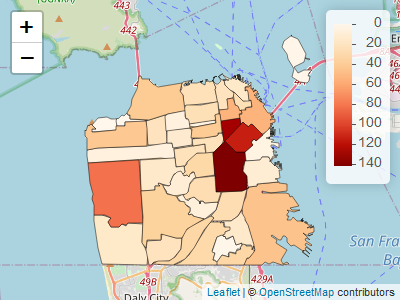
\includegraphics[width=0.9\linewidth]{crimebythenumbers_files/figure-latex/unnamed-chunk-23-1} \end{center}

By default \texttt{plot()} makes a scatterplot. If we set the parameter \texttt{type} to ``l'' it will be a \textbf{l}ine plot.

\begin{Shaded}
\begin{Highlighting}[]
\FunctionTok{plot}\NormalTok{(}\AttributeTok{x =}\NormalTok{ colorado\_agg}\SpecialCharTok{$}\NormalTok{year, }\AttributeTok{y =}\NormalTok{ colorado\_agg}\SpecialCharTok{$}\NormalTok{murder\_rate, }\AttributeTok{type =} \StringTok{"l"}\NormalTok{)}
\end{Highlighting}
\end{Shaded}

\begin{center}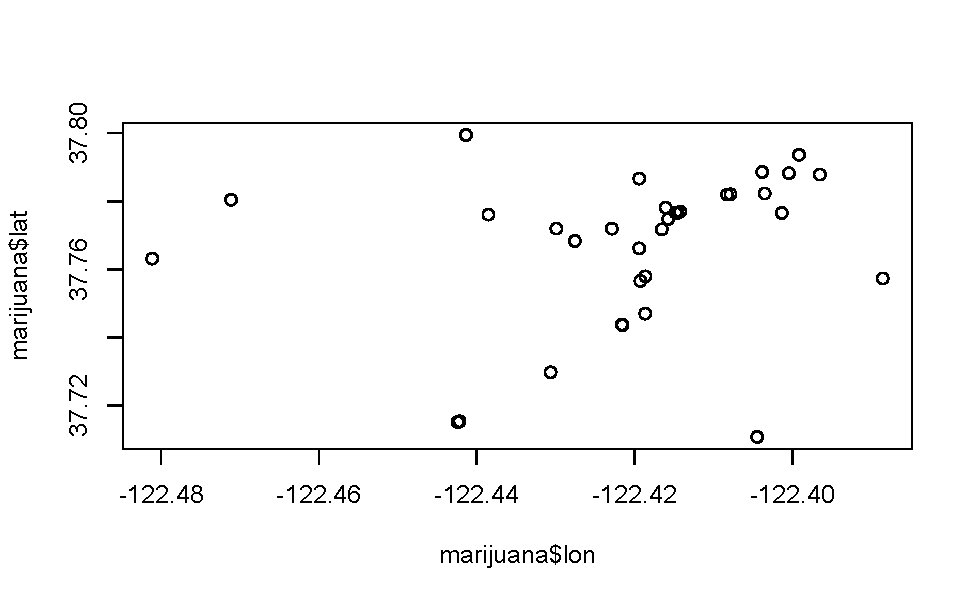
\includegraphics[width=0.9\linewidth]{crimebythenumbers_files/figure-latex/unnamed-chunk-24-1} \end{center}

We can add some labels and a title to make this graph easier to read.

\begin{Shaded}
\begin{Highlighting}[]
\FunctionTok{plot}\NormalTok{(}\AttributeTok{x =}\NormalTok{ colorado\_agg}\SpecialCharTok{$}\NormalTok{year, }\AttributeTok{y =}\NormalTok{ colorado\_agg}\SpecialCharTok{$}\NormalTok{murder\_rate, }\AttributeTok{type =} \StringTok{"l"}\NormalTok{,}
     \AttributeTok{xlab =} \StringTok{"Year"}\NormalTok{,}
     \AttributeTok{ylab =} \StringTok{"Murders per 100k Population"}\NormalTok{,}
     \AttributeTok{main =} \StringTok{"Murder Rate in Colorado, 2011{-}2017"}\NormalTok{)}
\end{Highlighting}
\end{Shaded}

\begin{center}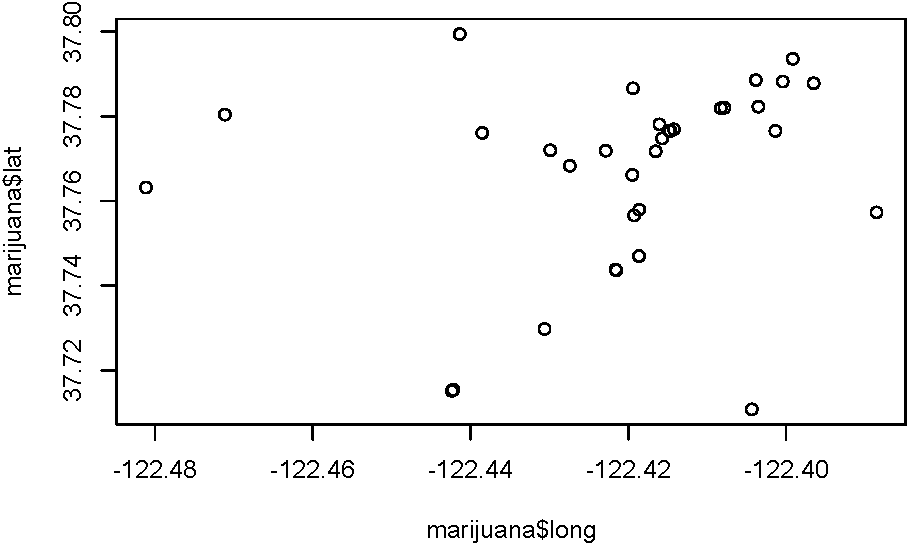
\includegraphics[width=0.9\linewidth]{crimebythenumbers_files/figure-latex/unnamed-chunk-25-1} \end{center}

\hypertarget{regular-expressions}{%
\chapter{Regular Expressions}\label{regular-expressions}}

Many word processing programs like Microsoft Word or Google Docs let you search for a pattern - usually a word or phrase - and it will show you where on the page that pattern appears. It also lets you replace that word or phrase with something new. R does the same using the function \texttt{grep()} to search for a pattern and tell you where in the data it appears, and \texttt{gsub()} which lets you search for a pattern and then replace it with a new pattern.

\begin{itemize}
\tightlist
\item
  \texttt{grep()} - Find
\item
  \texttt{gsub()} - Find and Replace
\end{itemize}

The \texttt{grep()} function lets you find a pattern in the text and it will return a number saying which element has the pattern (in a data.frame this tells you which row has a match). \texttt{gsub()} lets you input a pattern to find and a pattern to replace it with, just like Find and Replace features elsewhere. You can remember the difference because \texttt{gsub()} has the word ``sub'' in it and what it does is substitute text with new text.

A useful cheat sheet on regular expressions is available \href{https://www.rstudio.com/wp-content/uploads/2016/09/RegExCheatsheet.pdf}{here}.

For this lesson we will use a vector of 50 crime categories. These are all of the crimes in San Francisco Police data. As we'll see, there are some issues with the crime names that we need to fix.

\begin{Shaded}
\begin{Highlighting}[]
\NormalTok{crimes }\OtherTok{\textless{}{-}} \FunctionTok{c}\NormalTok{(}
  \StringTok{"Arson"}\NormalTok{,}
  \StringTok{"Assault"}\NormalTok{,                                  }
  \StringTok{"Burglary"}\NormalTok{,                                 }
  \StringTok{"Case Closure"}\NormalTok{,                             }
  \StringTok{"Civil Sidewalks"}\NormalTok{,                          }
  \StringTok{"Courtesy Report"}\NormalTok{,                          }
  \StringTok{"Disorderly Conduct"}\NormalTok{,                       }
  \StringTok{"Drug Offense"}\NormalTok{,                             }
  \StringTok{"Drug Violation"}\NormalTok{,                           }
  \StringTok{"Embezzlement"}\NormalTok{,                             }
  \StringTok{"Family Offense"}\NormalTok{,                           }
  \StringTok{"Fire Report"}\NormalTok{,                              }
  \StringTok{"Forgery And Counterfeiting"}\NormalTok{,               }
  \StringTok{"Fraud"}\NormalTok{,                                    }
  \StringTok{"Gambling"}\NormalTok{,                                 }
  \StringTok{"Homicide"}\NormalTok{,                                 }
  \StringTok{"Human Trafficking (A), Commercial Sex Acts"}\NormalTok{,}
  \StringTok{"Human Trafficking, Commercial Sex Acts"}\NormalTok{,   }
  \StringTok{"Juvenile Offenses"}\NormalTok{,                        }
  \StringTok{"Larceny Theft"}\NormalTok{,                            }
  \StringTok{"Liquor Laws"}\NormalTok{,                              }
  \StringTok{"Lost Property"}\NormalTok{,                            }
  \StringTok{"Malicious Mischief"}\NormalTok{,                       }
  \StringTok{"Miscellaneous Investigation"}\NormalTok{,              }
  \StringTok{"Missing Person"}\NormalTok{,                           }
  \StringTok{"Motor Vehicle Theft"}\NormalTok{,                      }
  \StringTok{"Motor Vehicle Theft?"}\NormalTok{,                     }
  \StringTok{"Non{-}Criminal"}\NormalTok{,                             }
  \StringTok{"Offences Against The Family And Children"}\NormalTok{, }
  \StringTok{"Other"}\NormalTok{,                                    }
  \StringTok{"Other Miscellaneous"}\NormalTok{,                      }
  \StringTok{"Other Offenses"}\NormalTok{,                           }
  \StringTok{"Prostitution"}\NormalTok{,                             }
  \StringTok{"Rape"}\NormalTok{,                                     }
  \StringTok{"Recovered Vehicle"}\NormalTok{,                        }
  \StringTok{"Robbery"}\NormalTok{,                                  }
  \StringTok{"Sex Offense"}\NormalTok{,                              }
  \StringTok{"Stolen Property"}\NormalTok{,                          }
  \StringTok{"Suicide"}\NormalTok{,                                  }
  \StringTok{"Suspicious"}\NormalTok{,                               }
  \StringTok{"Suspicious Occ"}\NormalTok{,                           }
  \StringTok{"Traffic Collision"}\NormalTok{,                        }
  \StringTok{"Traffic Violation Arrest"}\NormalTok{,                 }
  \StringTok{"Vandalism"}\NormalTok{,                                }
  \StringTok{"Vehicle Impounded"}\NormalTok{,                        }
  \StringTok{"Vehicle Misplaced"}\NormalTok{,                        }
  \StringTok{"Warrant"}\NormalTok{,                                  }
  \StringTok{"Weapons Carrying Etc"}\NormalTok{,                     }
  \StringTok{"Weapons Offence"}\NormalTok{,                          }
  \StringTok{"Weapons Offense"}
\NormalTok{)}
\end{Highlighting}
\end{Shaded}

When looking closely at these crimes it is clear that some may overlap in certain categories such as theft, and there are several duplicates with slight differences in spelling. For example the last two crimes are ``Weapons Offence'' and ``Weapons Offense''. These should be the same crime but the first one spelled ``offense'' wrong. And take a look at ``motor vehicle theft''. There are two crimes here because one of them adds a question mark at the end for some reason.

\hypertarget{finding-patterns-in-text-with-grep}{%
\section{\texorpdfstring{Finding patterns in text with \texttt{grep()}}{Finding patterns in text with grep()}}\label{finding-patterns-in-text-with-grep}}

We'll start with \texttt{grep()} which allows us to search a vector of data (in R, columns in a data.frame operate the same as a vector) and find where there is a match for the pattern we want to look for.

The syntax for \texttt{grep()} is

\texttt{grep("pattern",\ data)}

Where pattern is the pattern you are searching for, such as ``a'' if you want to find all values with the letter a. The pattern must always be in quotes. data is a vector of strings (such as \emph{crimes} we made above or a column in a data.frame) that you are searching in to find the pattern.

The output of this function is a number which says which element(s) in the vector the pattern was found in. If it returns, for example, the numbers 1 and 3 you know that the first and third element in your vector has the pattern - and no other elements do. It is essentially returning the index where the conditional statement ``is this pattern present'' is true.

So since our data is \emph{crimes} our \texttt{grep()} function will be \texttt{grep("",\ crimes)}. What we put in the "" is the pattern we want to search for.

Let's start with the letter ``a''.

\begin{Shaded}
\begin{Highlighting}[]
\FunctionTok{grep}\NormalTok{(}\StringTok{"a"}\NormalTok{, crimes)}
\CommentTok{\#\textgreater{}  [1]  2  3  4  5  9 11 14 15 17 18 20 21 23 24 28 29 31}
\CommentTok{\#\textgreater{} [18] 34 42 43 44 46 47 48 49 50}
\end{Highlighting}
\end{Shaded}

It gives us a bunch of numbers where the letter ``a'' is present in that element of \emph{crimes}. What this is useful for is subsetting. We can use \texttt{grep()} to find all values that match a pattern we want and subset to keep just those values.

\begin{Shaded}
\begin{Highlighting}[]
\NormalTok{crimes[}\FunctionTok{grep}\NormalTok{(}\StringTok{"a"}\NormalTok{, crimes)]}
\CommentTok{\#\textgreater{}  [1] "Assault"                                   }
\CommentTok{\#\textgreater{}  [2] "Burglary"                                  }
\CommentTok{\#\textgreater{}  [3] "Case Closure"                              }
\CommentTok{\#\textgreater{}  [4] "Civil Sidewalks"                           }
\CommentTok{\#\textgreater{}  [5] "Drug Violation"                            }
\CommentTok{\#\textgreater{}  [6] "Family Offense"                            }
\CommentTok{\#\textgreater{}  [7] "Fraud"                                     }
\CommentTok{\#\textgreater{}  [8] "Gambling"                                  }
\CommentTok{\#\textgreater{}  [9] "Human Trafficking (A), Commercial Sex Acts"}
\CommentTok{\#\textgreater{} [10] "Human Trafficking, Commercial Sex Acts"    }
\CommentTok{\#\textgreater{} [11] "Larceny Theft"                             }
\CommentTok{\#\textgreater{} [12] "Liquor Laws"                               }
\CommentTok{\#\textgreater{} [13] "Malicious Mischief"                        }
\CommentTok{\#\textgreater{} [14] "Miscellaneous Investigation"               }
\CommentTok{\#\textgreater{} [15] "Non{-}Criminal"                              }
\CommentTok{\#\textgreater{} [16] "Offences Against The Family And Children"  }
\CommentTok{\#\textgreater{} [17] "Other Miscellaneous"                       }
\CommentTok{\#\textgreater{} [18] "Rape"                                      }
\CommentTok{\#\textgreater{} [19] "Traffic Collision"                         }
\CommentTok{\#\textgreater{} [20] "Traffic Violation Arrest"                  }
\CommentTok{\#\textgreater{} [21] "Vandalism"                                 }
\CommentTok{\#\textgreater{} [22] "Vehicle Misplaced"                         }
\CommentTok{\#\textgreater{} [23] "Warrant"                                   }
\CommentTok{\#\textgreater{} [24] "Weapons Carrying Etc"                      }
\CommentTok{\#\textgreater{} [25] "Weapons Offence"                           }
\CommentTok{\#\textgreater{} [26] "Weapons Offense"}
\end{Highlighting}
\end{Shaded}

Searching for the letter ``a'' isn't that useful. Let's say we want to subset the data to only include theft related crimes. From reading the list of crimes we can see there are multiple theft crimes - ``Larceny Theft'', ``Motor Vehicle Theft'', and ``Motor Vehicle Theft?''. We may also want to include ``Stolen Property'' in this search but we'll wait until later in this lesson for how to search for multiple patterns. Since those three crimes all have the word ``Theft'' in the name we can search for the pattern and it will return only those crimes

\begin{Shaded}
\begin{Highlighting}[]
\FunctionTok{grep}\NormalTok{(}\StringTok{"Theft"}\NormalTok{, crimes)}
\CommentTok{\#\textgreater{} [1] 20 26 27}
\end{Highlighting}
\end{Shaded}

\begin{Shaded}
\begin{Highlighting}[]
\NormalTok{crimes[}\FunctionTok{grep}\NormalTok{(}\StringTok{"Theft"}\NormalTok{, crimes)]}
\CommentTok{\#\textgreater{} [1] "Larceny Theft"        "Motor Vehicle Theft" }
\CommentTok{\#\textgreater{} [3] "Motor Vehicle Theft?"}
\end{Highlighting}
\end{Shaded}

A very useful parameter is \texttt{value}. When we set \texttt{value} to TRUE, it will print out the actual strings that are a match rather than the element number. While this prevents us from using it to subset (since R no longer knows which rows are a match), it is an excellent tool to check if the \texttt{grep()} was successful as we can visually confirm it returns what we want. When we start to learn about special characters which make the patterns more complicated, this will be important.

\begin{Shaded}
\begin{Highlighting}[]
\FunctionTok{grep}\NormalTok{(}\StringTok{"Theft"}\NormalTok{, crimes, }\AttributeTok{value =} \ConstantTok{TRUE}\NormalTok{)}
\CommentTok{\#\textgreater{} [1] "Larceny Theft"        "Motor Vehicle Theft" }
\CommentTok{\#\textgreater{} [3] "Motor Vehicle Theft?"}
\end{Highlighting}
\end{Shaded}

Note that \texttt{grep()} (and \texttt{gsub()}) is case sensitive so you must capitalize properly.

\begin{Shaded}
\begin{Highlighting}[]
\FunctionTok{grep}\NormalTok{(}\StringTok{"theft"}\NormalTok{, }\AttributeTok{value =} \ConstantTok{TRUE}\NormalTok{, crimes)}
\CommentTok{\#\textgreater{} character(0)}
\end{Highlighting}
\end{Shaded}

Setting the parameter \texttt{ignore.case} to be TRUE makes \texttt{grep()} ignore capitalization.

\begin{Shaded}
\begin{Highlighting}[]
\FunctionTok{grep}\NormalTok{(}\StringTok{"theft"}\NormalTok{, crimes, }\AttributeTok{value =} \ConstantTok{TRUE}\NormalTok{, }\AttributeTok{ignore.case =} \ConstantTok{TRUE}\NormalTok{)}
\CommentTok{\#\textgreater{} [1] "Larceny Theft"        "Motor Vehicle Theft" }
\CommentTok{\#\textgreater{} [3] "Motor Vehicle Theft?"}
\end{Highlighting}
\end{Shaded}

If we want to find values which do \emph{not} match with ``theft'', we can set the parameter \texttt{invert} to TRUE.

\begin{Shaded}
\begin{Highlighting}[]
\FunctionTok{grep}\NormalTok{(}\StringTok{"theft"}\NormalTok{, crimes, }\AttributeTok{value =} \ConstantTok{TRUE}\NormalTok{, }\AttributeTok{ignore.case =} \ConstantTok{TRUE}\NormalTok{, }\AttributeTok{invert =} \ConstantTok{TRUE}\NormalTok{)}
\CommentTok{\#\textgreater{}  [1] "Arson"                                     }
\CommentTok{\#\textgreater{}  [2] "Assault"                                   }
\CommentTok{\#\textgreater{}  [3] "Burglary"                                  }
\CommentTok{\#\textgreater{}  [4] "Case Closure"                              }
\CommentTok{\#\textgreater{}  [5] "Civil Sidewalks"                           }
\CommentTok{\#\textgreater{}  [6] "Courtesy Report"                           }
\CommentTok{\#\textgreater{}  [7] "Disorderly Conduct"                        }
\CommentTok{\#\textgreater{}  [8] "Drug Offense"                              }
\CommentTok{\#\textgreater{}  [9] "Drug Violation"                            }
\CommentTok{\#\textgreater{} [10] "Embezzlement"                              }
\CommentTok{\#\textgreater{} [11] "Family Offense"                            }
\CommentTok{\#\textgreater{} [12] "Fire Report"                               }
\CommentTok{\#\textgreater{} [13] "Forgery And Counterfeiting"                }
\CommentTok{\#\textgreater{} [14] "Fraud"                                     }
\CommentTok{\#\textgreater{} [15] "Gambling"                                  }
\CommentTok{\#\textgreater{} [16] "Homicide"                                  }
\CommentTok{\#\textgreater{} [17] "Human Trafficking (A), Commercial Sex Acts"}
\CommentTok{\#\textgreater{} [18] "Human Trafficking, Commercial Sex Acts"    }
\CommentTok{\#\textgreater{} [19] "Juvenile Offenses"                         }
\CommentTok{\#\textgreater{} [20] "Liquor Laws"                               }
\CommentTok{\#\textgreater{} [21] "Lost Property"                             }
\CommentTok{\#\textgreater{} [22] "Malicious Mischief"                        }
\CommentTok{\#\textgreater{} [23] "Miscellaneous Investigation"               }
\CommentTok{\#\textgreater{} [24] "Missing Person"                            }
\CommentTok{\#\textgreater{} [25] "Non{-}Criminal"                              }
\CommentTok{\#\textgreater{} [26] "Offences Against The Family And Children"  }
\CommentTok{\#\textgreater{} [27] "Other"                                     }
\CommentTok{\#\textgreater{} [28] "Other Miscellaneous"                       }
\CommentTok{\#\textgreater{} [29] "Other Offenses"                            }
\CommentTok{\#\textgreater{} [30] "Prostitution"                              }
\CommentTok{\#\textgreater{} [31] "Rape"                                      }
\CommentTok{\#\textgreater{} [32] "Recovered Vehicle"                         }
\CommentTok{\#\textgreater{} [33] "Robbery"                                   }
\CommentTok{\#\textgreater{} [34] "Sex Offense"                               }
\CommentTok{\#\textgreater{} [35] "Stolen Property"                           }
\CommentTok{\#\textgreater{} [36] "Suicide"                                   }
\CommentTok{\#\textgreater{} [37] "Suspicious"                                }
\CommentTok{\#\textgreater{} [38] "Suspicious Occ"                            }
\CommentTok{\#\textgreater{} [39] "Traffic Collision"                         }
\CommentTok{\#\textgreater{} [40] "Traffic Violation Arrest"                  }
\CommentTok{\#\textgreater{} [41] "Vandalism"                                 }
\CommentTok{\#\textgreater{} [42] "Vehicle Impounded"                         }
\CommentTok{\#\textgreater{} [43] "Vehicle Misplaced"                         }
\CommentTok{\#\textgreater{} [44] "Warrant"                                   }
\CommentTok{\#\textgreater{} [45] "Weapons Carrying Etc"                      }
\CommentTok{\#\textgreater{} [46] "Weapons Offence"                           }
\CommentTok{\#\textgreater{} [47] "Weapons Offense"}
\end{Highlighting}
\end{Shaded}

\hypertarget{finding-and-replacing-patterns-in-text-with-gsub}{%
\section{\texorpdfstring{Finding and replacing patterns in text with \texttt{gsub()}}{Finding and replacing patterns in text with gsub()}}\label{finding-and-replacing-patterns-in-text-with-gsub}}

\texttt{gsub()} takes patterns and replaces them with other patterns. An important use in criminology for \texttt{gsub()} is to fix spelling mistakes in the text such as the way ``offense'' was spelled wrong in our data. This will be a standard part of your data cleaning process and is important as a misspelled word can cause significant issues. For example if our previous example of marijuana legalization in Colorado had half of agencies misspelling the name ``Colorado'', aggregating the data by the state (or simply subsetting to just Colorado agencies) would give completely different results as you'd lose half your data.

\texttt{gsub()} is also useful when you want to take subcategories and change the value to larger categories. For example we could take any crime with the word ``Theft'' in it and change the whole crime name to ``Theft''. In our data that would take 3 subcategories of thefts and turn it into a larger category we could aggregate to. This will be useful in city-level data where you may only care about a certain type of crime but it has many subcategories that you need to aggregate.

The syntax of \texttt{gsub()} is similar to \texttt{grep()} with the addition of a pattern to replace the pattern we found.

\texttt{gsub("find\_pattern",\ "replace\_pattern",\ data)}

Let's start with a simple example of finding the letter ``a'' and replacing it with ``z''. Our data will be the word ``cat''.

\begin{Shaded}
\begin{Highlighting}[]
\FunctionTok{gsub}\NormalTok{(}\StringTok{"a"}\NormalTok{, }\StringTok{"z"}\NormalTok{, }\StringTok{"cat"}\NormalTok{)}
\CommentTok{\#\textgreater{} [1] "czt"}
\end{Highlighting}
\end{Shaded}

Like \texttt{grep()}, \texttt{gsub()} is case sensitive and has the parameter \texttt{ignore.case} to ignore capitalization.

\begin{Shaded}
\begin{Highlighting}[]
\FunctionTok{gsub}\NormalTok{(}\StringTok{"A"}\NormalTok{, }\StringTok{"z"}\NormalTok{, }\StringTok{"cat"}\NormalTok{)}
\CommentTok{\#\textgreater{} [1] "cat"}
\end{Highlighting}
\end{Shaded}

\begin{Shaded}
\begin{Highlighting}[]
\FunctionTok{gsub}\NormalTok{(}\StringTok{"A"}\NormalTok{, }\StringTok{"z"}\NormalTok{, }\StringTok{"cat"}\NormalTok{, }\AttributeTok{ignore.case =} \ConstantTok{TRUE}\NormalTok{)}
\CommentTok{\#\textgreater{} [1] "czt"}
\end{Highlighting}
\end{Shaded}

\texttt{gsub()} returns the same data you input but with the pattern already replaced. Above you can see that when using capital A, it returns ``cat'' unchanged as it never found the pattern. When \texttt{ignore.case} was set to TRUE it returned ``czt'' as it then matched to letter ``A''.

We can use \texttt{gsub()} to replace some issues in the crimes data such as ``Offense'' being spelled ``Offence''.

\begin{Shaded}
\begin{Highlighting}[]
\FunctionTok{gsub}\NormalTok{(}\StringTok{"Offence"}\NormalTok{, }\StringTok{"Offense"}\NormalTok{, crimes)}
\CommentTok{\#\textgreater{}  [1] "Arson"                                     }
\CommentTok{\#\textgreater{}  [2] "Assault"                                   }
\CommentTok{\#\textgreater{}  [3] "Burglary"                                  }
\CommentTok{\#\textgreater{}  [4] "Case Closure"                              }
\CommentTok{\#\textgreater{}  [5] "Civil Sidewalks"                           }
\CommentTok{\#\textgreater{}  [6] "Courtesy Report"                           }
\CommentTok{\#\textgreater{}  [7] "Disorderly Conduct"                        }
\CommentTok{\#\textgreater{}  [8] "Drug Offense"                              }
\CommentTok{\#\textgreater{}  [9] "Drug Violation"                            }
\CommentTok{\#\textgreater{} [10] "Embezzlement"                              }
\CommentTok{\#\textgreater{} [11] "Family Offense"                            }
\CommentTok{\#\textgreater{} [12] "Fire Report"                               }
\CommentTok{\#\textgreater{} [13] "Forgery And Counterfeiting"                }
\CommentTok{\#\textgreater{} [14] "Fraud"                                     }
\CommentTok{\#\textgreater{} [15] "Gambling"                                  }
\CommentTok{\#\textgreater{} [16] "Homicide"                                  }
\CommentTok{\#\textgreater{} [17] "Human Trafficking (A), Commercial Sex Acts"}
\CommentTok{\#\textgreater{} [18] "Human Trafficking, Commercial Sex Acts"    }
\CommentTok{\#\textgreater{} [19] "Juvenile Offenses"                         }
\CommentTok{\#\textgreater{} [20] "Larceny Theft"                             }
\CommentTok{\#\textgreater{} [21] "Liquor Laws"                               }
\CommentTok{\#\textgreater{} [22] "Lost Property"                             }
\CommentTok{\#\textgreater{} [23] "Malicious Mischief"                        }
\CommentTok{\#\textgreater{} [24] "Miscellaneous Investigation"               }
\CommentTok{\#\textgreater{} [25] "Missing Person"                            }
\CommentTok{\#\textgreater{} [26] "Motor Vehicle Theft"                       }
\CommentTok{\#\textgreater{} [27] "Motor Vehicle Theft?"                      }
\CommentTok{\#\textgreater{} [28] "Non{-}Criminal"                              }
\CommentTok{\#\textgreater{} [29] "Offenses Against The Family And Children"  }
\CommentTok{\#\textgreater{} [30] "Other"                                     }
\CommentTok{\#\textgreater{} [31] "Other Miscellaneous"                       }
\CommentTok{\#\textgreater{} [32] "Other Offenses"                            }
\CommentTok{\#\textgreater{} [33] "Prostitution"                              }
\CommentTok{\#\textgreater{} [34] "Rape"                                      }
\CommentTok{\#\textgreater{} [35] "Recovered Vehicle"                         }
\CommentTok{\#\textgreater{} [36] "Robbery"                                   }
\CommentTok{\#\textgreater{} [37] "Sex Offense"                               }
\CommentTok{\#\textgreater{} [38] "Stolen Property"                           }
\CommentTok{\#\textgreater{} [39] "Suicide"                                   }
\CommentTok{\#\textgreater{} [40] "Suspicious"                                }
\CommentTok{\#\textgreater{} [41] "Suspicious Occ"                            }
\CommentTok{\#\textgreater{} [42] "Traffic Collision"                         }
\CommentTok{\#\textgreater{} [43] "Traffic Violation Arrest"                  }
\CommentTok{\#\textgreater{} [44] "Vandalism"                                 }
\CommentTok{\#\textgreater{} [45] "Vehicle Impounded"                         }
\CommentTok{\#\textgreater{} [46] "Vehicle Misplaced"                         }
\CommentTok{\#\textgreater{} [47] "Warrant"                                   }
\CommentTok{\#\textgreater{} [48] "Weapons Carrying Etc"                      }
\CommentTok{\#\textgreater{} [49] "Weapons Offense"                           }
\CommentTok{\#\textgreater{} [50] "Weapons Offense"}
\end{Highlighting}
\end{Shaded}

A useful pattern is an empty string "" which says replace whatever the find\_pattern is with nothing, deleting it. Let's delete the letter ``a'' (lowercase only) from the data.

\begin{Shaded}
\begin{Highlighting}[]
\FunctionTok{gsub}\NormalTok{(}\StringTok{"a"}\NormalTok{, }\StringTok{""}\NormalTok{, crimes)}
\CommentTok{\#\textgreater{}  [1] "Arson"                                  }
\CommentTok{\#\textgreater{}  [2] "Assult"                                 }
\CommentTok{\#\textgreater{}  [3] "Burglry"                                }
\CommentTok{\#\textgreater{}  [4] "Cse Closure"                            }
\CommentTok{\#\textgreater{}  [5] "Civil Sidewlks"                         }
\CommentTok{\#\textgreater{}  [6] "Courtesy Report"                        }
\CommentTok{\#\textgreater{}  [7] "Disorderly Conduct"                     }
\CommentTok{\#\textgreater{}  [8] "Drug Offense"                           }
\CommentTok{\#\textgreater{}  [9] "Drug Violtion"                          }
\CommentTok{\#\textgreater{} [10] "Embezzlement"                           }
\CommentTok{\#\textgreater{} [11] "Fmily Offense"                          }
\CommentTok{\#\textgreater{} [12] "Fire Report"                            }
\CommentTok{\#\textgreater{} [13] "Forgery And Counterfeiting"             }
\CommentTok{\#\textgreater{} [14] "Frud"                                   }
\CommentTok{\#\textgreater{} [15] "Gmbling"                                }
\CommentTok{\#\textgreater{} [16] "Homicide"                               }
\CommentTok{\#\textgreater{} [17] "Humn Trfficking (A), Commercil Sex Acts"}
\CommentTok{\#\textgreater{} [18] "Humn Trfficking, Commercil Sex Acts"    }
\CommentTok{\#\textgreater{} [19] "Juvenile Offenses"                      }
\CommentTok{\#\textgreater{} [20] "Lrceny Theft"                           }
\CommentTok{\#\textgreater{} [21] "Liquor Lws"                             }
\CommentTok{\#\textgreater{} [22] "Lost Property"                          }
\CommentTok{\#\textgreater{} [23] "Mlicious Mischief"                      }
\CommentTok{\#\textgreater{} [24] "Miscellneous Investigtion"              }
\CommentTok{\#\textgreater{} [25] "Missing Person"                         }
\CommentTok{\#\textgreater{} [26] "Motor Vehicle Theft"                    }
\CommentTok{\#\textgreater{} [27] "Motor Vehicle Theft?"                   }
\CommentTok{\#\textgreater{} [28] "Non{-}Criminl"                            }
\CommentTok{\#\textgreater{} [29] "Offences Aginst The Fmily And Children" }
\CommentTok{\#\textgreater{} [30] "Other"                                  }
\CommentTok{\#\textgreater{} [31] "Other Miscellneous"                     }
\CommentTok{\#\textgreater{} [32] "Other Offenses"                         }
\CommentTok{\#\textgreater{} [33] "Prostitution"                           }
\CommentTok{\#\textgreater{} [34] "Rpe"                                    }
\CommentTok{\#\textgreater{} [35] "Recovered Vehicle"                      }
\CommentTok{\#\textgreater{} [36] "Robbery"                                }
\CommentTok{\#\textgreater{} [37] "Sex Offense"                            }
\CommentTok{\#\textgreater{} [38] "Stolen Property"                        }
\CommentTok{\#\textgreater{} [39] "Suicide"                                }
\CommentTok{\#\textgreater{} [40] "Suspicious"                             }
\CommentTok{\#\textgreater{} [41] "Suspicious Occ"                         }
\CommentTok{\#\textgreater{} [42] "Trffic Collision"                       }
\CommentTok{\#\textgreater{} [43] "Trffic Violtion Arrest"                 }
\CommentTok{\#\textgreater{} [44] "Vndlism"                                }
\CommentTok{\#\textgreater{} [45] "Vehicle Impounded"                      }
\CommentTok{\#\textgreater{} [46] "Vehicle Misplced"                       }
\CommentTok{\#\textgreater{} [47] "Wrrnt"                                  }
\CommentTok{\#\textgreater{} [48] "Wepons Crrying Etc"                     }
\CommentTok{\#\textgreater{} [49] "Wepons Offence"                         }
\CommentTok{\#\textgreater{} [50] "Wepons Offense"}
\end{Highlighting}
\end{Shaded}

\hypertarget{useful-special-characters}{%
\section{Useful special characters}\label{useful-special-characters}}

So far, we have just searched for a single character or word and expected a return only if an exact match was found. Now we'll discuss a number of characters called ``special characters'' that allow us to make more complex \texttt{grep()} and \texttt{gsub()} pattern searches.

\hypertarget{multiple-characters}{%
\subsection{\texorpdfstring{Multiple characters \texttt{{[}{]}}}{Multiple characters {[}{]}}}\label{multiple-characters}}

To search for multiple matches we can put the pattern we want to search for inside square brackets \texttt{{[}{]}} (note that we use the same square brackets for subsetting but they operate very differently in this context). For example, we can find all the crimes that contain the letters ``x'', ``y'', or ``z''.

The \texttt{grep()} searches if any of the letters inside of the \texttt{{[}{]}} are present in our \emph{crimes} vector.

\begin{Shaded}
\begin{Highlighting}[]
\FunctionTok{grep}\NormalTok{(}\StringTok{"[xyz]"}\NormalTok{, crimes, }\AttributeTok{value =} \ConstantTok{TRUE}\NormalTok{)}
\CommentTok{\#\textgreater{}  [1] "Burglary"                                  }
\CommentTok{\#\textgreater{}  [2] "Courtesy Report"                           }
\CommentTok{\#\textgreater{}  [3] "Disorderly Conduct"                        }
\CommentTok{\#\textgreater{}  [4] "Embezzlement"                              }
\CommentTok{\#\textgreater{}  [5] "Family Offense"                            }
\CommentTok{\#\textgreater{}  [6] "Forgery And Counterfeiting"                }
\CommentTok{\#\textgreater{}  [7] "Human Trafficking (A), Commercial Sex Acts"}
\CommentTok{\#\textgreater{}  [8] "Human Trafficking, Commercial Sex Acts"    }
\CommentTok{\#\textgreater{}  [9] "Larceny Theft"                             }
\CommentTok{\#\textgreater{} [10] "Lost Property"                             }
\CommentTok{\#\textgreater{} [11] "Offences Against The Family And Children"  }
\CommentTok{\#\textgreater{} [12] "Robbery"                                   }
\CommentTok{\#\textgreater{} [13] "Sex Offense"                               }
\CommentTok{\#\textgreater{} [14] "Stolen Property"                           }
\CommentTok{\#\textgreater{} [15] "Weapons Carrying Etc"}
\end{Highlighting}
\end{Shaded}

As it searches for any letter inside of the square brackets, the order does not matter.

\begin{Shaded}
\begin{Highlighting}[]
\FunctionTok{grep}\NormalTok{(}\StringTok{"[zyx]"}\NormalTok{, crimes, }\AttributeTok{value =} \ConstantTok{TRUE}\NormalTok{)}
\CommentTok{\#\textgreater{}  [1] "Burglary"                                  }
\CommentTok{\#\textgreater{}  [2] "Courtesy Report"                           }
\CommentTok{\#\textgreater{}  [3] "Disorderly Conduct"                        }
\CommentTok{\#\textgreater{}  [4] "Embezzlement"                              }
\CommentTok{\#\textgreater{}  [5] "Family Offense"                            }
\CommentTok{\#\textgreater{}  [6] "Forgery And Counterfeiting"                }
\CommentTok{\#\textgreater{}  [7] "Human Trafficking (A), Commercial Sex Acts"}
\CommentTok{\#\textgreater{}  [8] "Human Trafficking, Commercial Sex Acts"    }
\CommentTok{\#\textgreater{}  [9] "Larceny Theft"                             }
\CommentTok{\#\textgreater{} [10] "Lost Property"                             }
\CommentTok{\#\textgreater{} [11] "Offences Against The Family And Children"  }
\CommentTok{\#\textgreater{} [12] "Robbery"                                   }
\CommentTok{\#\textgreater{} [13] "Sex Offense"                               }
\CommentTok{\#\textgreater{} [14] "Stolen Property"                           }
\CommentTok{\#\textgreater{} [15] "Weapons Carrying Etc"}
\end{Highlighting}
\end{Shaded}

This also works for numbers though we do not have any numbers in the data.

\begin{Shaded}
\begin{Highlighting}[]
\FunctionTok{grep}\NormalTok{(}\StringTok{"[01234567890]"}\NormalTok{, crimes, }\AttributeTok{value =} \ConstantTok{TRUE}\NormalTok{)}
\CommentTok{\#\textgreater{} character(0)}
\end{Highlighting}
\end{Shaded}

If we wanted to search for a pattern, such as vowels, that is repeated we could put multiple \texttt{{[}{]}} patterns together. We will see another way to search for a repeated pattern soon.

\begin{Shaded}
\begin{Highlighting}[]
\FunctionTok{grep}\NormalTok{(}\StringTok{"[aeiou][aeiou][aeiou]"}\NormalTok{, crimes, }\AttributeTok{value =} \ConstantTok{TRUE}\NormalTok{)}
\CommentTok{\#\textgreater{} [1] "Malicious Mischief"         }
\CommentTok{\#\textgreater{} [2] "Miscellaneous Investigation"}
\CommentTok{\#\textgreater{} [3] "Other Miscellaneous"        }
\CommentTok{\#\textgreater{} [4] "Suspicious"                 }
\CommentTok{\#\textgreater{} [5] "Suspicious Occ"}
\end{Highlighting}
\end{Shaded}

Inside the \texttt{{[}{]}} we can also use the - to make intervals between certain values. For numbers, n-m means any number between n and m (inclusive). For letters, a-z means all lowercase letters and A-Z means all uppercase letters in that range (inclusive).

\begin{Shaded}
\begin{Highlighting}[]
\FunctionTok{grep}\NormalTok{(}\StringTok{"[x{-}z]"}\NormalTok{, crimes, }\AttributeTok{value =} \ConstantTok{TRUE}\NormalTok{)}
\CommentTok{\#\textgreater{}  [1] "Burglary"                                  }
\CommentTok{\#\textgreater{}  [2] "Courtesy Report"                           }
\CommentTok{\#\textgreater{}  [3] "Disorderly Conduct"                        }
\CommentTok{\#\textgreater{}  [4] "Embezzlement"                              }
\CommentTok{\#\textgreater{}  [5] "Family Offense"                            }
\CommentTok{\#\textgreater{}  [6] "Forgery And Counterfeiting"                }
\CommentTok{\#\textgreater{}  [7] "Human Trafficking (A), Commercial Sex Acts"}
\CommentTok{\#\textgreater{}  [8] "Human Trafficking, Commercial Sex Acts"    }
\CommentTok{\#\textgreater{}  [9] "Larceny Theft"                             }
\CommentTok{\#\textgreater{} [10] "Lost Property"                             }
\CommentTok{\#\textgreater{} [11] "Offences Against The Family And Children"  }
\CommentTok{\#\textgreater{} [12] "Robbery"                                   }
\CommentTok{\#\textgreater{} [13] "Sex Offense"                               }
\CommentTok{\#\textgreater{} [14] "Stolen Property"                           }
\CommentTok{\#\textgreater{} [15] "Weapons Carrying Etc"}
\end{Highlighting}
\end{Shaded}

\hypertarget{n-many-of-previous-character-n}{%
\subsection{\texorpdfstring{n-many of previous character \texttt{\{n\}}}{n-many of previous character \{n\}}}\label{n-many-of-previous-character-n}}

\texttt{\{n\}} means the preceding item will be matched exactly n times.

We can use it to rewrite the above \texttt{grep()} to saw the values in the \texttt{{[}{]}} should be repeated three times.

\begin{Shaded}
\begin{Highlighting}[]
\FunctionTok{grep}\NormalTok{(}\StringTok{"[aeiou]\{3\}"}\NormalTok{, crimes, }\AttributeTok{value =} \ConstantTok{TRUE}\NormalTok{)}
\CommentTok{\#\textgreater{} [1] "Malicious Mischief"         }
\CommentTok{\#\textgreater{} [2] "Miscellaneous Investigation"}
\CommentTok{\#\textgreater{} [3] "Other Miscellaneous"        }
\CommentTok{\#\textgreater{} [4] "Suspicious"                 }
\CommentTok{\#\textgreater{} [5] "Suspicious Occ"}
\end{Highlighting}
\end{Shaded}

\hypertarget{n-many-to-m-many-of-previous-character-nm}{%
\subsection{\texorpdfstring{n-many to m-many of previous character \texttt{\{n,m\}}}{n-many to m-many of previous character \{n,m\}}}\label{n-many-to-m-many-of-previous-character-nm}}

While \texttt{\{n\}} says ``the previous character (or characters inside a \texttt{{[}{]}}) must be present exactly n times'', we can allow a range by using \texttt{\{n,m\}}. Here the previous character must be present between n and m times.

We can check for values where there are 2-3 vowels in a row. Note that there cannot be a space before or after the comma.

\begin{Shaded}
\begin{Highlighting}[]
\FunctionTok{grep}\NormalTok{(}\StringTok{"[aeiou]\{2,3\}"}\NormalTok{, crimes, }\AttributeTok{value =} \ConstantTok{TRUE}\NormalTok{)}
\CommentTok{\#\textgreater{}  [1] "Assault"                                   }
\CommentTok{\#\textgreater{}  [2] "Courtesy Report"                           }
\CommentTok{\#\textgreater{}  [3] "Drug Violation"                            }
\CommentTok{\#\textgreater{}  [4] "Forgery And Counterfeiting"                }
\CommentTok{\#\textgreater{}  [5] "Fraud"                                     }
\CommentTok{\#\textgreater{}  [6] "Human Trafficking (A), Commercial Sex Acts"}
\CommentTok{\#\textgreater{}  [7] "Human Trafficking, Commercial Sex Acts"    }
\CommentTok{\#\textgreater{}  [8] "Liquor Laws"                               }
\CommentTok{\#\textgreater{}  [9] "Malicious Mischief"                        }
\CommentTok{\#\textgreater{} [10] "Miscellaneous Investigation"               }
\CommentTok{\#\textgreater{} [11] "Offences Against The Family And Children"  }
\CommentTok{\#\textgreater{} [12] "Other Miscellaneous"                       }
\CommentTok{\#\textgreater{} [13] "Prostitution"                              }
\CommentTok{\#\textgreater{} [14] "Suicide"                                   }
\CommentTok{\#\textgreater{} [15] "Suspicious"                                }
\CommentTok{\#\textgreater{} [16] "Suspicious Occ"                            }
\CommentTok{\#\textgreater{} [17] "Traffic Collision"                         }
\CommentTok{\#\textgreater{} [18] "Traffic Violation Arrest"                  }
\CommentTok{\#\textgreater{} [19] "Vehicle Impounded"                         }
\CommentTok{\#\textgreater{} [20] "Weapons Carrying Etc"                      }
\CommentTok{\#\textgreater{} [21] "Weapons Offence"                           }
\CommentTok{\#\textgreater{} [22] "Weapons Offense"}
\end{Highlighting}
\end{Shaded}

If we wanted only crimes with exactly three vowels in a row we'd use \texttt{\{3,3\}}.

\begin{Shaded}
\begin{Highlighting}[]
\FunctionTok{grep}\NormalTok{(}\StringTok{"[aeiou]\{3,3\}"}\NormalTok{, crimes, }\AttributeTok{value =} \ConstantTok{TRUE}\NormalTok{)}
\CommentTok{\#\textgreater{} [1] "Malicious Mischief"         }
\CommentTok{\#\textgreater{} [2] "Miscellaneous Investigation"}
\CommentTok{\#\textgreater{} [3] "Other Miscellaneous"        }
\CommentTok{\#\textgreater{} [4] "Suspicious"                 }
\CommentTok{\#\textgreater{} [5] "Suspicious Occ"}
\end{Highlighting}
\end{Shaded}

If we leave n blank, such as \texttt{\{,m\}} it says, ``previous character must be present up to m times.''

\begin{Shaded}
\begin{Highlighting}[]
\FunctionTok{grep}\NormalTok{(}\StringTok{"[aeiou]\{,3\}"}\NormalTok{, crimes, }\AttributeTok{value =} \ConstantTok{TRUE}\NormalTok{)}
\CommentTok{\#\textgreater{}  [1] "Arson"                                     }
\CommentTok{\#\textgreater{}  [2] "Assault"                                   }
\CommentTok{\#\textgreater{}  [3] "Burglary"                                  }
\CommentTok{\#\textgreater{}  [4] "Case Closure"                              }
\CommentTok{\#\textgreater{}  [5] "Civil Sidewalks"                           }
\CommentTok{\#\textgreater{}  [6] "Courtesy Report"                           }
\CommentTok{\#\textgreater{}  [7] "Disorderly Conduct"                        }
\CommentTok{\#\textgreater{}  [8] "Drug Offense"                              }
\CommentTok{\#\textgreater{}  [9] "Drug Violation"                            }
\CommentTok{\#\textgreater{} [10] "Embezzlement"                              }
\CommentTok{\#\textgreater{} [11] "Family Offense"                            }
\CommentTok{\#\textgreater{} [12] "Fire Report"                               }
\CommentTok{\#\textgreater{} [13] "Forgery And Counterfeiting"                }
\CommentTok{\#\textgreater{} [14] "Fraud"                                     }
\CommentTok{\#\textgreater{} [15] "Gambling"                                  }
\CommentTok{\#\textgreater{} [16] "Homicide"                                  }
\CommentTok{\#\textgreater{} [17] "Human Trafficking (A), Commercial Sex Acts"}
\CommentTok{\#\textgreater{} [18] "Human Trafficking, Commercial Sex Acts"    }
\CommentTok{\#\textgreater{} [19] "Juvenile Offenses"                         }
\CommentTok{\#\textgreater{} [20] "Larceny Theft"                             }
\CommentTok{\#\textgreater{} [21] "Liquor Laws"                               }
\CommentTok{\#\textgreater{} [22] "Lost Property"                             }
\CommentTok{\#\textgreater{} [23] "Malicious Mischief"                        }
\CommentTok{\#\textgreater{} [24] "Miscellaneous Investigation"               }
\CommentTok{\#\textgreater{} [25] "Missing Person"                            }
\CommentTok{\#\textgreater{} [26] "Motor Vehicle Theft"                       }
\CommentTok{\#\textgreater{} [27] "Motor Vehicle Theft?"                      }
\CommentTok{\#\textgreater{} [28] "Non{-}Criminal"                              }
\CommentTok{\#\textgreater{} [29] "Offences Against The Family And Children"  }
\CommentTok{\#\textgreater{} [30] "Other"                                     }
\CommentTok{\#\textgreater{} [31] "Other Miscellaneous"                       }
\CommentTok{\#\textgreater{} [32] "Other Offenses"                            }
\CommentTok{\#\textgreater{} [33] "Prostitution"                              }
\CommentTok{\#\textgreater{} [34] "Rape"                                      }
\CommentTok{\#\textgreater{} [35] "Recovered Vehicle"                         }
\CommentTok{\#\textgreater{} [36] "Robbery"                                   }
\CommentTok{\#\textgreater{} [37] "Sex Offense"                               }
\CommentTok{\#\textgreater{} [38] "Stolen Property"                           }
\CommentTok{\#\textgreater{} [39] "Suicide"                                   }
\CommentTok{\#\textgreater{} [40] "Suspicious"                                }
\CommentTok{\#\textgreater{} [41] "Suspicious Occ"                            }
\CommentTok{\#\textgreater{} [42] "Traffic Collision"                         }
\CommentTok{\#\textgreater{} [43] "Traffic Violation Arrest"                  }
\CommentTok{\#\textgreater{} [44] "Vandalism"                                 }
\CommentTok{\#\textgreater{} [45] "Vehicle Impounded"                         }
\CommentTok{\#\textgreater{} [46] "Vehicle Misplaced"                         }
\CommentTok{\#\textgreater{} [47] "Warrant"                                   }
\CommentTok{\#\textgreater{} [48] "Weapons Carrying Etc"                      }
\CommentTok{\#\textgreater{} [49] "Weapons Offence"                           }
\CommentTok{\#\textgreater{} [50] "Weapons Offense"}
\end{Highlighting}
\end{Shaded}

This returns every crime as ``up to m times'' includes zero times.

And the same works for leaving m blank but it will be ``present at least n times''.

\begin{Shaded}
\begin{Highlighting}[]
\FunctionTok{grep}\NormalTok{(}\StringTok{"[aeiou]\{3,\}"}\NormalTok{, crimes, }\AttributeTok{value =} \ConstantTok{TRUE}\NormalTok{)}
\CommentTok{\#\textgreater{} [1] "Malicious Mischief"         }
\CommentTok{\#\textgreater{} [2] "Miscellaneous Investigation"}
\CommentTok{\#\textgreater{} [3] "Other Miscellaneous"        }
\CommentTok{\#\textgreater{} [4] "Suspicious"                 }
\CommentTok{\#\textgreater{} [5] "Suspicious Occ"}
\end{Highlighting}
\end{Shaded}

\hypertarget{start-of-string}{%
\subsection{Start of string}\label{start-of-string}}

The \texttt{\^{}} symbol (called a caret) signifies that what follows it is the start of the string. We put the \texttt{\^{}} at the beginning of the quotes and then anything that follows it must be the very start of the string. As an example let's search for ``Family''. Our data has both the ``Family Offense'' crime and the ``Offences Against The Family And Children'' crime (which likely are the same crime written differently). If we use \texttt{\^{}} then we should only have the first one returned.

\begin{Shaded}
\begin{Highlighting}[]
\FunctionTok{grep}\NormalTok{(}\StringTok{"\^{}Family"}\NormalTok{, crimes, }\AttributeTok{value =} \ConstantTok{TRUE}\NormalTok{)}
\CommentTok{\#\textgreater{} [1] "Family Offense"}
\end{Highlighting}
\end{Shaded}

\hypertarget{end-of-string}{%
\subsection{\texorpdfstring{End of string \texttt{\$}}{End of string \$}}\label{end-of-string}}

The dollar sign \texttt{\$} acts similar to the caret \texttt{\^{}} except that it signifies that the value before it is the \textbf{end} of the string. We put the \texttt{\$} at the very end of our search pattern and whatever character is before it is the end of the string. For example, let's search for all crimes that end with the word ``Theft''.

\begin{Shaded}
\begin{Highlighting}[]
\FunctionTok{grep}\NormalTok{(}\StringTok{"Theft$"}\NormalTok{, crimes, }\AttributeTok{value =} \ConstantTok{TRUE}\NormalTok{)}
\CommentTok{\#\textgreater{} [1] "Larceny Theft"       "Motor Vehicle Theft"}
\end{Highlighting}
\end{Shaded}

Note that the crime ``Motor Vehicle Theft?'' doesn't get selected as it ends with a question mark.

\hypertarget{anything-.}{%
\subsection{\texorpdfstring{Anything \texttt{.}}{Anything .}}\label{anything-.}}

The \texttt{.} symbol is a stand-in for any value. This is useful when you aren't sure about every part of the pattern you are searching. It can also be used when there are slight differences in words such as our incorrect ``Offence'' and ``Offense''. We can replace the ``c'' and ``s'' with the \texttt{.}.

\begin{Shaded}
\begin{Highlighting}[]
\FunctionTok{grep}\NormalTok{(}\StringTok{"Weapons Offen.e"}\NormalTok{, crimes, }\AttributeTok{value =} \ConstantTok{TRUE}\NormalTok{)}
\CommentTok{\#\textgreater{} [1] "Weapons Offence" "Weapons Offense"}
\end{Highlighting}
\end{Shaded}

\hypertarget{one-or-more-of-previous}{%
\subsection{\texorpdfstring{One or more of previous \texttt{+}}{One or more of previous +}}\label{one-or-more-of-previous}}

The \texttt{+} means that the character immediately before it is present at least one time. This is the same as writing \texttt{\{1,\}}. If we wanted to find all values with only two words, we would start with some number of letters followed by a space followed by some more letters and the string would end.

\begin{Shaded}
\begin{Highlighting}[]
\FunctionTok{grep}\NormalTok{(}\StringTok{"\^{}[A{-}Za{-}z]+ [A{-}Za{-}z]+$"}\NormalTok{, crimes, }\AttributeTok{value =} \ConstantTok{TRUE}\NormalTok{)}
\CommentTok{\#\textgreater{}  [1] "Case Closure"               }
\CommentTok{\#\textgreater{}  [2] "Civil Sidewalks"            }
\CommentTok{\#\textgreater{}  [3] "Courtesy Report"            }
\CommentTok{\#\textgreater{}  [4] "Disorderly Conduct"         }
\CommentTok{\#\textgreater{}  [5] "Drug Offense"               }
\CommentTok{\#\textgreater{}  [6] "Drug Violation"             }
\CommentTok{\#\textgreater{}  [7] "Family Offense"             }
\CommentTok{\#\textgreater{}  [8] "Fire Report"                }
\CommentTok{\#\textgreater{}  [9] "Juvenile Offenses"          }
\CommentTok{\#\textgreater{} [10] "Larceny Theft"              }
\CommentTok{\#\textgreater{} [11] "Liquor Laws"                }
\CommentTok{\#\textgreater{} [12] "Lost Property"              }
\CommentTok{\#\textgreater{} [13] "Malicious Mischief"         }
\CommentTok{\#\textgreater{} [14] "Miscellaneous Investigation"}
\CommentTok{\#\textgreater{} [15] "Missing Person"             }
\CommentTok{\#\textgreater{} [16] "Other Miscellaneous"        }
\CommentTok{\#\textgreater{} [17] "Other Offenses"             }
\CommentTok{\#\textgreater{} [18] "Recovered Vehicle"          }
\CommentTok{\#\textgreater{} [19] "Sex Offense"                }
\CommentTok{\#\textgreater{} [20] "Stolen Property"            }
\CommentTok{\#\textgreater{} [21] "Suspicious Occ"             }
\CommentTok{\#\textgreater{} [22] "Traffic Collision"          }
\CommentTok{\#\textgreater{} [23] "Vehicle Impounded"          }
\CommentTok{\#\textgreater{} [24] "Vehicle Misplaced"          }
\CommentTok{\#\textgreater{} [25] "Weapons Offence"            }
\CommentTok{\#\textgreater{} [26] "Weapons Offense"}
\end{Highlighting}
\end{Shaded}

\hypertarget{zero-or-more-of-previous}{%
\subsection{\texorpdfstring{Zero or more of previous \texttt{*}}{Zero or more of previous *}}\label{zero-or-more-of-previous}}

The \texttt{*} special character says match zero or more of the previous character and is the same as \texttt{\{0,\}}. Combining \texttt{.} with \texttt{*} is powerful when used in \texttt{gsub()} to delete text before or after a pattern. Let's write a pattern that searches the text for the word ``Weapons'' and then deletes any text after that.

Our pattern would be "Weapons.*" which is the word ``Weapons'' followed by anything zero or more times.

\begin{Shaded}
\begin{Highlighting}[]
\FunctionTok{gsub}\NormalTok{(}\StringTok{"Weapons.*"}\NormalTok{, }\StringTok{"Weapons"}\NormalTok{, crimes)}
\CommentTok{\#\textgreater{}  [1] "Arson"                                     }
\CommentTok{\#\textgreater{}  [2] "Assault"                                   }
\CommentTok{\#\textgreater{}  [3] "Burglary"                                  }
\CommentTok{\#\textgreater{}  [4] "Case Closure"                              }
\CommentTok{\#\textgreater{}  [5] "Civil Sidewalks"                           }
\CommentTok{\#\textgreater{}  [6] "Courtesy Report"                           }
\CommentTok{\#\textgreater{}  [7] "Disorderly Conduct"                        }
\CommentTok{\#\textgreater{}  [8] "Drug Offense"                              }
\CommentTok{\#\textgreater{}  [9] "Drug Violation"                            }
\CommentTok{\#\textgreater{} [10] "Embezzlement"                              }
\CommentTok{\#\textgreater{} [11] "Family Offense"                            }
\CommentTok{\#\textgreater{} [12] "Fire Report"                               }
\CommentTok{\#\textgreater{} [13] "Forgery And Counterfeiting"                }
\CommentTok{\#\textgreater{} [14] "Fraud"                                     }
\CommentTok{\#\textgreater{} [15] "Gambling"                                  }
\CommentTok{\#\textgreater{} [16] "Homicide"                                  }
\CommentTok{\#\textgreater{} [17] "Human Trafficking (A), Commercial Sex Acts"}
\CommentTok{\#\textgreater{} [18] "Human Trafficking, Commercial Sex Acts"    }
\CommentTok{\#\textgreater{} [19] "Juvenile Offenses"                         }
\CommentTok{\#\textgreater{} [20] "Larceny Theft"                             }
\CommentTok{\#\textgreater{} [21] "Liquor Laws"                               }
\CommentTok{\#\textgreater{} [22] "Lost Property"                             }
\CommentTok{\#\textgreater{} [23] "Malicious Mischief"                        }
\CommentTok{\#\textgreater{} [24] "Miscellaneous Investigation"               }
\CommentTok{\#\textgreater{} [25] "Missing Person"                            }
\CommentTok{\#\textgreater{} [26] "Motor Vehicle Theft"                       }
\CommentTok{\#\textgreater{} [27] "Motor Vehicle Theft?"                      }
\CommentTok{\#\textgreater{} [28] "Non{-}Criminal"                              }
\CommentTok{\#\textgreater{} [29] "Offences Against The Family And Children"  }
\CommentTok{\#\textgreater{} [30] "Other"                                     }
\CommentTok{\#\textgreater{} [31] "Other Miscellaneous"                       }
\CommentTok{\#\textgreater{} [32] "Other Offenses"                            }
\CommentTok{\#\textgreater{} [33] "Prostitution"                              }
\CommentTok{\#\textgreater{} [34] "Rape"                                      }
\CommentTok{\#\textgreater{} [35] "Recovered Vehicle"                         }
\CommentTok{\#\textgreater{} [36] "Robbery"                                   }
\CommentTok{\#\textgreater{} [37] "Sex Offense"                               }
\CommentTok{\#\textgreater{} [38] "Stolen Property"                           }
\CommentTok{\#\textgreater{} [39] "Suicide"                                   }
\CommentTok{\#\textgreater{} [40] "Suspicious"                                }
\CommentTok{\#\textgreater{} [41] "Suspicious Occ"                            }
\CommentTok{\#\textgreater{} [42] "Traffic Collision"                         }
\CommentTok{\#\textgreater{} [43] "Traffic Violation Arrest"                  }
\CommentTok{\#\textgreater{} [44] "Vandalism"                                 }
\CommentTok{\#\textgreater{} [45] "Vehicle Impounded"                         }
\CommentTok{\#\textgreater{} [46] "Vehicle Misplaced"                         }
\CommentTok{\#\textgreater{} [47] "Warrant"                                   }
\CommentTok{\#\textgreater{} [48] "Weapons"                                   }
\CommentTok{\#\textgreater{} [49] "Weapons"                                   }
\CommentTok{\#\textgreater{} [50] "Weapons"}
\end{Highlighting}
\end{Shaded}

And now our last three crimes are all identical.

\hypertarget{multiple-patterns}{%
\subsection{\texorpdfstring{Multiple patterns \texttt{\textbar{}}}{Multiple patterns \textbar{}}}\label{multiple-patterns}}

The vertical bar \texttt{\textbar{}} special character allows us to check for multiple patterns. It essentially functions as ``pattern A or Pattern B'' with the \texttt{\textbar{}} symbol replacing the word ``or'' (and making sure to not have any space between patterns.). To check our crimes for the word ``Drug'' or the word ``Weapons'' we could write ``Drug\textbar Weapon'' which searches for ``Drug'' or ``Weapons'' in the text.

\begin{Shaded}
\begin{Highlighting}[]
\FunctionTok{grep}\NormalTok{(}\StringTok{"Drug|Weapons"}\NormalTok{, crimes, }\AttributeTok{value =} \ConstantTok{TRUE}\NormalTok{)}
\CommentTok{\#\textgreater{} [1] "Drug Offense"         "Drug Violation"      }
\CommentTok{\#\textgreater{} [3] "Weapons Carrying Etc" "Weapons Offence"     }
\CommentTok{\#\textgreater{} [5] "Weapons Offense"}
\end{Highlighting}
\end{Shaded}

\hypertarget{parentheses}{%
\subsection{\texorpdfstring{Parentheses \texttt{()}}{Parentheses ()}}\label{parentheses}}

Parentheses act similar to the square brackets \texttt{{[}{]}} where we want everything inside but with parentheses the values must be in the proper order.

\begin{Shaded}
\begin{Highlighting}[]
\FunctionTok{grep}\NormalTok{(}\StringTok{"(Offense)"}\NormalTok{, crimes, }\AttributeTok{value =} \ConstantTok{TRUE}\NormalTok{)}
\CommentTok{\#\textgreater{} [1] "Drug Offense"      "Family Offense"   }
\CommentTok{\#\textgreater{} [3] "Juvenile Offenses" "Other Offenses"   }
\CommentTok{\#\textgreater{} [5] "Sex Offense"       "Weapons Offense"}
\end{Highlighting}
\end{Shaded}

Running the above code returns the same results as if we didn't include the parentheses. The usefulness of parentheses comes when combining it with the \texttt{\textbar{}} symbol to be able to check ``(X\textbar Y) Z''), which says, ``look for either X or Y which must be followed by Z''.

Running just ``(Offense)'' returns values for multiple types of offenses. Let's say we just care about Drug and Weapon Offenses. We can search for ``Offense'' normally and combine \texttt{()} and \texttt{\textbar{}} to say, ``search for either the word''Drug" or the word ``Family'' and they should be followed by the word ``Offense''.

\begin{Shaded}
\begin{Highlighting}[]
\FunctionTok{grep}\NormalTok{(}\StringTok{"(Drug|Weapons) Offense"}\NormalTok{, crimes, }\AttributeTok{value =} \ConstantTok{TRUE}\NormalTok{)}
\CommentTok{\#\textgreater{} [1] "Drug Offense"    "Weapons Offense"}
\end{Highlighting}
\end{Shaded}

\hypertarget{optional-text}{%
\subsection{\texorpdfstring{Optional text \texttt{?}}{Optional text ?}}\label{optional-text}}

The question mark indicates that the character immediately before the \texttt{?} is optional.

Let's search for the term ``offens'' and add a ? at the end. This says search for the pattern ``offen'' and we expect an exact match for that pattern. And if the letter ``s'' follows ``offen'' return that too, but it isn't required to be there.

\begin{Shaded}
\begin{Highlighting}[]
\FunctionTok{grep}\NormalTok{(}\StringTok{"Offens?"}\NormalTok{, crimes, }\AttributeTok{value =} \ConstantTok{TRUE}\NormalTok{)}
\CommentTok{\#\textgreater{} [1] "Drug Offense"                            }
\CommentTok{\#\textgreater{} [2] "Family Offense"                          }
\CommentTok{\#\textgreater{} [3] "Juvenile Offenses"                       }
\CommentTok{\#\textgreater{} [4] "Offences Against The Family And Children"}
\CommentTok{\#\textgreater{} [5] "Other Offenses"                          }
\CommentTok{\#\textgreater{} [6] "Sex Offense"                             }
\CommentTok{\#\textgreater{} [7] "Weapons Offence"                         }
\CommentTok{\#\textgreater{} [8] "Weapons Offense"}
\end{Highlighting}
\end{Shaded}

We can further combine it with \texttt{()} and \texttt{\textbar{}} to get both spellings of Weapon Offense.

\begin{Shaded}
\begin{Highlighting}[]
\FunctionTok{grep}\NormalTok{(}\StringTok{"(Drug|Weapons) Offens?"}\NormalTok{, crimes, }\AttributeTok{value =} \ConstantTok{TRUE}\NormalTok{)}
\CommentTok{\#\textgreater{} [1] "Drug Offense"    "Weapons Offence"}
\CommentTok{\#\textgreater{} [3] "Weapons Offense"}
\end{Highlighting}
\end{Shaded}

\hypertarget{changing-capitalization}{%
\section{Changing capitalization}\label{changing-capitalization}}

If you're dealing with data where the only difference is capitalization (as is common in crime data) instead of using \texttt{gsub()} to change individual values, you can use the functions \texttt{toupper()} and \texttt{tolower()} to change every letter's capitalization. These functions take as an input a vector of strings (or a column from a data.frame) and return those strings either upper or lowercase.

\begin{Shaded}
\begin{Highlighting}[]
\FunctionTok{toupper}\NormalTok{(crimes)}
\CommentTok{\#\textgreater{}  [1] "ARSON"                                     }
\CommentTok{\#\textgreater{}  [2] "ASSAULT"                                   }
\CommentTok{\#\textgreater{}  [3] "BURGLARY"                                  }
\CommentTok{\#\textgreater{}  [4] "CASE CLOSURE"                              }
\CommentTok{\#\textgreater{}  [5] "CIVIL SIDEWALKS"                           }
\CommentTok{\#\textgreater{}  [6] "COURTESY REPORT"                           }
\CommentTok{\#\textgreater{}  [7] "DISORDERLY CONDUCT"                        }
\CommentTok{\#\textgreater{}  [8] "DRUG OFFENSE"                              }
\CommentTok{\#\textgreater{}  [9] "DRUG VIOLATION"                            }
\CommentTok{\#\textgreater{} [10] "EMBEZZLEMENT"                              }
\CommentTok{\#\textgreater{} [11] "FAMILY OFFENSE"                            }
\CommentTok{\#\textgreater{} [12] "FIRE REPORT"                               }
\CommentTok{\#\textgreater{} [13] "FORGERY AND COUNTERFEITING"                }
\CommentTok{\#\textgreater{} [14] "FRAUD"                                     }
\CommentTok{\#\textgreater{} [15] "GAMBLING"                                  }
\CommentTok{\#\textgreater{} [16] "HOMICIDE"                                  }
\CommentTok{\#\textgreater{} [17] "HUMAN TRAFFICKING (A), COMMERCIAL SEX ACTS"}
\CommentTok{\#\textgreater{} [18] "HUMAN TRAFFICKING, COMMERCIAL SEX ACTS"    }
\CommentTok{\#\textgreater{} [19] "JUVENILE OFFENSES"                         }
\CommentTok{\#\textgreater{} [20] "LARCENY THEFT"                             }
\CommentTok{\#\textgreater{} [21] "LIQUOR LAWS"                               }
\CommentTok{\#\textgreater{} [22] "LOST PROPERTY"                             }
\CommentTok{\#\textgreater{} [23] "MALICIOUS MISCHIEF"                        }
\CommentTok{\#\textgreater{} [24] "MISCELLANEOUS INVESTIGATION"               }
\CommentTok{\#\textgreater{} [25] "MISSING PERSON"                            }
\CommentTok{\#\textgreater{} [26] "MOTOR VEHICLE THEFT"                       }
\CommentTok{\#\textgreater{} [27] "MOTOR VEHICLE THEFT?"                      }
\CommentTok{\#\textgreater{} [28] "NON{-}CRIMINAL"                              }
\CommentTok{\#\textgreater{} [29] "OFFENCES AGAINST THE FAMILY AND CHILDREN"  }
\CommentTok{\#\textgreater{} [30] "OTHER"                                     }
\CommentTok{\#\textgreater{} [31] "OTHER MISCELLANEOUS"                       }
\CommentTok{\#\textgreater{} [32] "OTHER OFFENSES"                            }
\CommentTok{\#\textgreater{} [33] "PROSTITUTION"                              }
\CommentTok{\#\textgreater{} [34] "RAPE"                                      }
\CommentTok{\#\textgreater{} [35] "RECOVERED VEHICLE"                         }
\CommentTok{\#\textgreater{} [36] "ROBBERY"                                   }
\CommentTok{\#\textgreater{} [37] "SEX OFFENSE"                               }
\CommentTok{\#\textgreater{} [38] "STOLEN PROPERTY"                           }
\CommentTok{\#\textgreater{} [39] "SUICIDE"                                   }
\CommentTok{\#\textgreater{} [40] "SUSPICIOUS"                                }
\CommentTok{\#\textgreater{} [41] "SUSPICIOUS OCC"                            }
\CommentTok{\#\textgreater{} [42] "TRAFFIC COLLISION"                         }
\CommentTok{\#\textgreater{} [43] "TRAFFIC VIOLATION ARREST"                  }
\CommentTok{\#\textgreater{} [44] "VANDALISM"                                 }
\CommentTok{\#\textgreater{} [45] "VEHICLE IMPOUNDED"                         }
\CommentTok{\#\textgreater{} [46] "VEHICLE MISPLACED"                         }
\CommentTok{\#\textgreater{} [47] "WARRANT"                                   }
\CommentTok{\#\textgreater{} [48] "WEAPONS CARRYING ETC"                      }
\CommentTok{\#\textgreater{} [49] "WEAPONS OFFENCE"                           }
\CommentTok{\#\textgreater{} [50] "WEAPONS OFFENSE"}
\end{Highlighting}
\end{Shaded}

\begin{Shaded}
\begin{Highlighting}[]
\FunctionTok{tolower}\NormalTok{(crimes)}
\CommentTok{\#\textgreater{}  [1] "arson"                                     }
\CommentTok{\#\textgreater{}  [2] "assault"                                   }
\CommentTok{\#\textgreater{}  [3] "burglary"                                  }
\CommentTok{\#\textgreater{}  [4] "case closure"                              }
\CommentTok{\#\textgreater{}  [5] "civil sidewalks"                           }
\CommentTok{\#\textgreater{}  [6] "courtesy report"                           }
\CommentTok{\#\textgreater{}  [7] "disorderly conduct"                        }
\CommentTok{\#\textgreater{}  [8] "drug offense"                              }
\CommentTok{\#\textgreater{}  [9] "drug violation"                            }
\CommentTok{\#\textgreater{} [10] "embezzlement"                              }
\CommentTok{\#\textgreater{} [11] "family offense"                            }
\CommentTok{\#\textgreater{} [12] "fire report"                               }
\CommentTok{\#\textgreater{} [13] "forgery and counterfeiting"                }
\CommentTok{\#\textgreater{} [14] "fraud"                                     }
\CommentTok{\#\textgreater{} [15] "gambling"                                  }
\CommentTok{\#\textgreater{} [16] "homicide"                                  }
\CommentTok{\#\textgreater{} [17] "human trafficking (a), commercial sex acts"}
\CommentTok{\#\textgreater{} [18] "human trafficking, commercial sex acts"    }
\CommentTok{\#\textgreater{} [19] "juvenile offenses"                         }
\CommentTok{\#\textgreater{} [20] "larceny theft"                             }
\CommentTok{\#\textgreater{} [21] "liquor laws"                               }
\CommentTok{\#\textgreater{} [22] "lost property"                             }
\CommentTok{\#\textgreater{} [23] "malicious mischief"                        }
\CommentTok{\#\textgreater{} [24] "miscellaneous investigation"               }
\CommentTok{\#\textgreater{} [25] "missing person"                            }
\CommentTok{\#\textgreater{} [26] "motor vehicle theft"                       }
\CommentTok{\#\textgreater{} [27] "motor vehicle theft?"                      }
\CommentTok{\#\textgreater{} [28] "non{-}criminal"                              }
\CommentTok{\#\textgreater{} [29] "offences against the family and children"  }
\CommentTok{\#\textgreater{} [30] "other"                                     }
\CommentTok{\#\textgreater{} [31] "other miscellaneous"                       }
\CommentTok{\#\textgreater{} [32] "other offenses"                            }
\CommentTok{\#\textgreater{} [33] "prostitution"                              }
\CommentTok{\#\textgreater{} [34] "rape"                                      }
\CommentTok{\#\textgreater{} [35] "recovered vehicle"                         }
\CommentTok{\#\textgreater{} [36] "robbery"                                   }
\CommentTok{\#\textgreater{} [37] "sex offense"                               }
\CommentTok{\#\textgreater{} [38] "stolen property"                           }
\CommentTok{\#\textgreater{} [39] "suicide"                                   }
\CommentTok{\#\textgreater{} [40] "suspicious"                                }
\CommentTok{\#\textgreater{} [41] "suspicious occ"                            }
\CommentTok{\#\textgreater{} [42] "traffic collision"                         }
\CommentTok{\#\textgreater{} [43] "traffic violation arrest"                  }
\CommentTok{\#\textgreater{} [44] "vandalism"                                 }
\CommentTok{\#\textgreater{} [45] "vehicle impounded"                         }
\CommentTok{\#\textgreater{} [46] "vehicle misplaced"                         }
\CommentTok{\#\textgreater{} [47] "warrant"                                   }
\CommentTok{\#\textgreater{} [48] "weapons carrying etc"                      }
\CommentTok{\#\textgreater{} [49] "weapons offence"                           }
\CommentTok{\#\textgreater{} [50] "weapons offense"}
\end{Highlighting}
\end{Shaded}

\hypertarget{reading-and-writing-data}{%
\chapter{Reading and Writing Data}\label{reading-and-writing-data}}

So far in these lessons we've used data from a number of sources but which all came as .rda files which is the standard R data format. Many data sets, particularly older government data, will not come as .rda file but rather as Excel, Stata, SAS, SPSS, or fixed-width ASCII files. In this brief lesson we'll cover how to read these formats into R as well as how to save data into these formats. Since many criminologists do not use R, it is important to be able to save the data in the language they use to be able to collaborate with them.

Fixed-width ASCII files are not very common and require a bit more effort than the other formats so we'll leave those until later to discuss.

In this lesson we'll use data about officer-involved shootings.

\hypertarget{reading-data-into-r-1}{%
\section{Reading Data into R}\label{reading-data-into-r-1}}

\hypertarget{r}{%
\subsection{R}\label{r}}

As we've seen earlier, to read in data with a .rda or .rdata extension you use the function \texttt{load()} with the file name (including the extension) in quotation marks inside of the parentheses. This loads the data into R and calls the object the name it was when it was saved. Therefore we do not need to give it a name ourselves.

For each of the other types of data we'll need to assign a name to the data we're reading in so it has a name. Whereas we've done \texttt{x\ \textless{}-\ 2} to say \emph{x} gets the value of 2, now we'd do \texttt{x\ \textless{}-\ DATA} where DATA is the way to load in the data and \emph{x} will get the entire data.frame that is read in.

\hypertarget{excel}{%
\subsection{Excel}\label{excel}}

To read in Excel files, those ending in .csv, we can use the function \texttt{read\_csv()} from the package \texttt{readr} (the function \texttt{read.csv()} is included in R by default so it doesn't require any packages but is far slower than \texttt{read\_csv()} so we will not use it).

\begin{Shaded}
\begin{Highlighting}[]
\FunctionTok{install.packages}\NormalTok{(}\StringTok{"readr"}\NormalTok{)}
\end{Highlighting}
\end{Shaded}

\begin{Shaded}
\begin{Highlighting}[]
\FunctionTok{library}\NormalTok{(readr)}
\end{Highlighting}
\end{Shaded}

The input in the () is the file name ending in ``.csv''. As it is telling R to read a file that is stored on your computer, the whole name must be in quotes. Unlike loading an .rda file using \texttt{load()}, there is no name for the object that gets read in so we must assign the data a name. We can use the name \emph{shootings} as it's relatively descriptive and easy for us to write.

\begin{Shaded}
\begin{Highlighting}[]
\NormalTok{shootings }\OtherTok{\textless{}{-}} \FunctionTok{read\_csv}\NormalTok{(}\StringTok{"data/fatal{-}police{-}shootings{-}data.csv"}\NormalTok{)}
\CommentTok{\#\textgreater{} }
\CommentTok{\#\textgreater{} {-}{-} Column specification {-}{-}{-}{-}{-}{-}{-}{-}{-}{-}{-}{-}{-}{-}{-}{-}{-}{-}{-}{-}{-}{-}{-}{-}{-}{-}{-}{-}{-}{-}{-}{-}}
\CommentTok{\#\textgreater{} cols(}
\CommentTok{\#\textgreater{}   id = col\_double(),}
\CommentTok{\#\textgreater{}   name = col\_character(),}
\CommentTok{\#\textgreater{}   date = col\_date(format = ""),}
\CommentTok{\#\textgreater{}   manner\_of\_death = col\_character(),}
\CommentTok{\#\textgreater{}   armed = col\_character(),}
\CommentTok{\#\textgreater{}   age = col\_double(),}
\CommentTok{\#\textgreater{}   gender = col\_character(),}
\CommentTok{\#\textgreater{}   race = col\_character(),}
\CommentTok{\#\textgreater{}   city = col\_character(),}
\CommentTok{\#\textgreater{}   state = col\_character(),}
\CommentTok{\#\textgreater{}   signs\_of\_mental\_illness = col\_logical(),}
\CommentTok{\#\textgreater{}   threat\_level = col\_character(),}
\CommentTok{\#\textgreater{}   flee = col\_character(),}
\CommentTok{\#\textgreater{}   body\_camera = col\_logical()}
\CommentTok{\#\textgreater{} )}
\end{Highlighting}
\end{Shaded}

\texttt{read\_csv()} also reads in data to an object called a \texttt{tibble} which is very similar to a data.frame but has some differences in displaying the data. If we run \texttt{head()} on the data it doesn't show all columns. This is useful to avoid accidentally printing out a massive amounts of columns.

\begin{Shaded}
\begin{Highlighting}[]
\FunctionTok{head}\NormalTok{(shootings)}
\CommentTok{\#\textgreater{} \# A tibble: 6 x 14}
\CommentTok{\#\textgreater{}      id name     date       manner\_of\_death armed    age}
\CommentTok{\#\textgreater{}   \textless{}dbl\textgreater{} \textless{}chr\textgreater{}    \textless{}date\textgreater{}     \textless{}chr\textgreater{}           \textless{}chr\textgreater{}  \textless{}dbl\textgreater{}}
\CommentTok{\#\textgreater{} 1     3 Tim Ell\textasciitilde{} 2015{-}01{-}02 shot            gun       53}
\CommentTok{\#\textgreater{} 2     4 Lewis L\textasciitilde{} 2015{-}01{-}02 shot            gun       47}
\CommentTok{\#\textgreater{} 3     5 John Pa\textasciitilde{} 2015{-}01{-}03 shot and Taser\textasciitilde{} unarm\textasciitilde{}    23}
\CommentTok{\#\textgreater{} 4     8 Matthew\textasciitilde{} 2015{-}01{-}04 shot            toy w\textasciitilde{}    32}
\CommentTok{\#\textgreater{} 5     9 Michael\textasciitilde{} 2015{-}01{-}04 shot            nail \textasciitilde{}    39}
\CommentTok{\#\textgreater{} 6    11 Kenneth\textasciitilde{} 2015{-}01{-}04 shot            gun       18}
\CommentTok{\#\textgreater{} \# ... with 8 more variables: gender \textless{}chr\textgreater{}, race \textless{}chr\textgreater{},}
\CommentTok{\#\textgreater{} \#   city \textless{}chr\textgreater{}, state \textless{}chr\textgreater{},}
\CommentTok{\#\textgreater{} \#   signs\_of\_mental\_illness \textless{}lgl\textgreater{}, threat\_level \textless{}chr\textgreater{},}
\CommentTok{\#\textgreater{} \#   flee \textless{}chr\textgreater{}, body\_camera \textless{}lgl\textgreater{}}
\end{Highlighting}
\end{Shaded}

We can convert it to a data.frame using the function \texttt{as.data.frame()} though that isn't strictly necessary since tibbles and data.frames operate so similarly.

\begin{Shaded}
\begin{Highlighting}[]
\NormalTok{shootings }\OtherTok{\textless{}{-}} \FunctionTok{as.data.frame}\NormalTok{(shootings)}
\end{Highlighting}
\end{Shaded}

\hypertarget{stata}{%
\subsection{Stata}\label{stata}}

For the remaining three data types we'll use the package \texttt{haven}.

\begin{Shaded}
\begin{Highlighting}[]
\FunctionTok{install.packages}\NormalTok{(}\StringTok{"haven"}\NormalTok{)}
\end{Highlighting}
\end{Shaded}

\begin{Shaded}
\begin{Highlighting}[]
\FunctionTok{library}\NormalTok{(haven)}
\end{Highlighting}
\end{Shaded}

\texttt{haven} follows the same syntax for each data type and is the same as with \texttt{read\_csv()} - for each data type we simply include the file name (in quotes, with the extension) and designate an name to be assigned the data.

Like with \texttt{read\_csv()} the functions to read data through \texttt{haven} all start with \texttt{read\_} and end with the extension you're reading in.

\begin{itemize}
\tightlist
\item
  \texttt{read\_dta()} - Stata file, extension ``dta''
\item
  \texttt{read\_sas()} - SAS file, extension ``sas''
\item
  \texttt{read\_sav()} - SPSS file, extension ``sav''
\end{itemize}

To read the data as a .dta format we can copy the code to read it as a .csv but change .csv to .dta.

\begin{Shaded}
\begin{Highlighting}[]
\NormalTok{shootings }\OtherTok{\textless{}{-}} \FunctionTok{read\_dta}\NormalTok{(}\StringTok{"data/fatal{-}police{-}shootings{-}data.dta"}\NormalTok{)}
\end{Highlighting}
\end{Shaded}

Since we called this new data \emph{shootings}, R overwrote that object (without warning us!). This is useful because we often want to subset or aggregate data and call it by the same name to avoid making too many objects to keep track of, but watch out for accidentally overwriting an object without noticing!

\hypertarget{sas}{%
\subsection{SAS}\label{sas}}

\begin{Shaded}
\begin{Highlighting}[]
\NormalTok{shootings }\OtherTok{\textless{}{-}} \FunctionTok{read\_sas}\NormalTok{(}\StringTok{"data/fatal{-}police{-}shootings{-}data.sas"}\NormalTok{)}
\end{Highlighting}
\end{Shaded}

\hypertarget{spss}{%
\subsection{SPSS}\label{spss}}

\begin{Shaded}
\begin{Highlighting}[]
\NormalTok{shootings }\OtherTok{\textless{}{-}} \FunctionTok{read\_sav}\NormalTok{(}\StringTok{"data/fatal{-}police{-}shootings{-}data.sav"}\NormalTok{)}
\end{Highlighting}
\end{Shaded}

\hypertarget{writing-data}{%
\section{Writing Data}\label{writing-data}}

When we're done with a project (or an important part of a project) or when we need to send data to someone, we need to save the data we've worked on in a suitable format. For each format, we are saving the data in we will follow the same syntax of

\texttt{function\_name(data,\ "file\_name")}

As usual we start with the function name. Then inside the parentheses we have the name of the object we are saving (as it refers to an object in R, we do not use quotations) and then the file name, in quotes, ending with the extension you want.

For saving an .rda file we use the \texttt{save()} function, otherwise we follow the syntax of \texttt{write\_} ending with the file extension.

\begin{itemize}
\tightlist
\item
  \texttt{write\_csv()} - Excel file, extension ``csv''
\item
  \texttt{write\_dta()} - Stata file, extension ``dta''
\item
  \texttt{write\_sas()} - SAS file, extension ``sas''
\item
  \texttt{write\_sav()} - SPSS file, extension ``sav''
\end{itemize}

As with reading the data, \texttt{write\_csv()} comes from the \texttt{readr} package while the other formats are from the \texttt{haven} package.

\hypertarget{r-1}{%
\subsection{R}\label{r-1}}

For saving an .rda file we must set the parameter \texttt{file} to be the name we're saving. For the other types of data they use the parameter \texttt{path} rather than \texttt{file} but it is not necessary to call them explicitly.

\begin{Shaded}
\begin{Highlighting}[]
\FunctionTok{save}\NormalTok{(shootings, }\AttributeTok{file =}  \StringTok{"data/shootings.rda"}\NormalTok{)}
\end{Highlighting}
\end{Shaded}

\hypertarget{excel-1}{%
\subsection{Excel}\label{excel-1}}

\begin{Shaded}
\begin{Highlighting}[]
\FunctionTok{write\_csv}\NormalTok{(shootings, }\StringTok{"data/shootings.csv"}\NormalTok{)}
\end{Highlighting}
\end{Shaded}

\hypertarget{stata-1}{%
\subsection{Stata}\label{stata-1}}

\begin{Shaded}
\begin{Highlighting}[]
\FunctionTok{write\_dta}\NormalTok{(shootings, }\StringTok{"data/shootings.dta"}\NormalTok{)}
\end{Highlighting}
\end{Shaded}

\hypertarget{sas-1}{%
\subsection{SAS}\label{sas-1}}

\begin{Shaded}
\begin{Highlighting}[]
\FunctionTok{write\_sas}\NormalTok{(shootings, }\StringTok{"data/shootings.sas"}\NormalTok{)}
\end{Highlighting}
\end{Shaded}

\hypertarget{spss-1}{%
\subsection{SPSS}\label{spss-1}}

\begin{Shaded}
\begin{Highlighting}[]
\FunctionTok{write\_sav}\NormalTok{(shootings, }\StringTok{"data/shootings.sav"}\NormalTok{)}
\end{Highlighting}
\end{Shaded}

\hypertarget{part-visualize}{%
\part{Visualize}\label{part-visualize}}

\hypertarget{graphing-intro}{%
\chapter{\texorpdfstring{Graphing with \texttt{ggplot2}}{Graphing with ggplot2}}\label{graphing-intro}}

We've made some simple graphs earlier; in this lesson we will use the package \texttt{ggplot2} to make simple and elegant looking graphs.

The `gg' part of \texttt{ggplot2} stands for `grammar of graphics' which is the idea that most graphs can be made using the same few `pieces.' We'll get into those pieces during this lesson. For a useful cheat sheet for this package see \href{https://www.rstudio.com/wp-content/uploads/2015/03/ggplot2-cheatsheet.pdf}{here}

\begin{Shaded}
\begin{Highlighting}[]
\FunctionTok{install.packages}\NormalTok{(}\StringTok{"ggplot2"}\NormalTok{)}
\end{Highlighting}
\end{Shaded}

\begin{Shaded}
\begin{Highlighting}[]
\FunctionTok{library}\NormalTok{(ggplot2)}
\end{Highlighting}
\end{Shaded}

When working with new data, It's often useful to quickly graph the data to try to understand what you're working with. It is also useful when understanding how much to trust the data.

The data we will work on is data about alcohol consumption in U.S. states from 1977-2017 from the National Institute of Health. It contains the per capita alcohol consumption for each state for every year. Their method to determine per capita consumption is amount of alcohol sold / number of people aged 14+ living in the state. More details on the data are available \href{https://www.openicpsr.org/openicpsr/project/105583/version/V2/view}{here}.

Now we need to load the data.

\begin{Shaded}
\begin{Highlighting}[]
\FunctionTok{load}\NormalTok{(}\StringTok{"data/apparent\_per\_capita\_alcohol\_consumption.rda"}\NormalTok{)}
\end{Highlighting}
\end{Shaded}

The name of the data is quite long so for convenience let's copy it to a new object with a better name, \emph{alcohol}.

\begin{Shaded}
\begin{Highlighting}[]
\NormalTok{alcohol }\OtherTok{\textless{}{-}}\NormalTok{ apparent\_per\_capita\_alcohol\_consumption}
\end{Highlighting}
\end{Shaded}

The original data has every state, region, and the US as a whole. For this lesson we're using data subsetted to just include states. For now let's just look at Pennsylvania.

\begin{Shaded}
\begin{Highlighting}[]
\NormalTok{penn\_alcohol }\OtherTok{\textless{}{-}}\NormalTok{ alcohol[alcohol}\SpecialCharTok{$}\NormalTok{state }\SpecialCharTok{==} \StringTok{"pennsylvania"}\NormalTok{, ]}
\end{Highlighting}
\end{Shaded}

\hypertarget{what-does-the-data-look-like}{%
\section{What does the data look like?}\label{what-does-the-data-look-like}}

Before graphing, it's helpful to see what the data includes. An important thing to check is what variables are available and the units of these variables.

\begin{Shaded}
\begin{Highlighting}[]
\FunctionTok{names}\NormalTok{(penn\_alcohol)}
\CommentTok{\#\textgreater{}  [1] "state"                                }
\CommentTok{\#\textgreater{}  [2] "year"                                 }
\CommentTok{\#\textgreater{}  [3] "ethanol\_beer\_gallons\_per\_capita"      }
\CommentTok{\#\textgreater{}  [4] "ethanol\_wine\_gallons\_per\_capita"      }
\CommentTok{\#\textgreater{}  [5] "ethanol\_spirit\_gallons\_per\_capita"    }
\CommentTok{\#\textgreater{}  [6] "ethanol\_all\_drinks\_gallons\_per\_capita"}
\CommentTok{\#\textgreater{}  [7] "number\_of\_beers"                      }
\CommentTok{\#\textgreater{}  [8] "number\_of\_glasses\_wine"               }
\CommentTok{\#\textgreater{}  [9] "number\_of\_shots\_liquor"               }
\CommentTok{\#\textgreater{} [10] "number\_of\_drinks\_total"}
\end{Highlighting}
\end{Shaded}

\begin{Shaded}
\begin{Highlighting}[]
\FunctionTok{summary}\NormalTok{(penn\_alcohol)}
\CommentTok{\#\textgreater{}     state               year          }
\CommentTok{\#\textgreater{}  Length:41          Length:41         }
\CommentTok{\#\textgreater{}  Class :character   Class :character  }
\CommentTok{\#\textgreater{}  Mode  :character   Mode  :character  }
\CommentTok{\#\textgreater{}                                       }
\CommentTok{\#\textgreater{}                                       }
\CommentTok{\#\textgreater{}                                       }
\CommentTok{\#\textgreater{}  ethanol\_beer\_gallons\_per\_capita}
\CommentTok{\#\textgreater{}  Min.   :1.210                  }
\CommentTok{\#\textgreater{}  1st Qu.:1.310                  }
\CommentTok{\#\textgreater{}  Median :1.350                  }
\CommentTok{\#\textgreater{}  Mean   :1.344                  }
\CommentTok{\#\textgreater{}  3rd Qu.:1.380                  }
\CommentTok{\#\textgreater{}  Max.   :1.450                  }
\CommentTok{\#\textgreater{}  ethanol\_wine\_gallons\_per\_capita}
\CommentTok{\#\textgreater{}  Min.   :0.1700                 }
\CommentTok{\#\textgreater{}  1st Qu.:0.1900                 }
\CommentTok{\#\textgreater{}  Median :0.2100                 }
\CommentTok{\#\textgreater{}  Mean   :0.2276                 }
\CommentTok{\#\textgreater{}  3rd Qu.:0.2500                 }
\CommentTok{\#\textgreater{}  Max.   :0.3300                 }
\CommentTok{\#\textgreater{}  ethanol\_spirit\_gallons\_per\_capita}
\CommentTok{\#\textgreater{}  Min.   :0.4500                   }
\CommentTok{\#\textgreater{}  1st Qu.:0.5100                   }
\CommentTok{\#\textgreater{}  Median :0.6100                   }
\CommentTok{\#\textgreater{}  Mean   :0.5939                   }
\CommentTok{\#\textgreater{}  3rd Qu.:0.6800                   }
\CommentTok{\#\textgreater{}  Max.   :0.7400                   }
\CommentTok{\#\textgreater{}  ethanol\_all\_drinks\_gallons\_per\_capita number\_of\_beers}
\CommentTok{\#\textgreater{}  Min.   :1.850                         Min.   :286.8  }
\CommentTok{\#\textgreater{}  1st Qu.:2.040                         1st Qu.:310.5  }
\CommentTok{\#\textgreater{}  Median :2.220                         Median :320.0  }
\CommentTok{\#\textgreater{}  Mean   :2.167                         Mean   :318.7  }
\CommentTok{\#\textgreater{}  3rd Qu.:2.330                         3rd Qu.:327.1  }
\CommentTok{\#\textgreater{}  Max.   :2.390                         Max.   :343.7  }
\CommentTok{\#\textgreater{}  number\_of\_glasses\_wine number\_of\_shots\_liquor}
\CommentTok{\#\textgreater{}  Min.   :33.74          Min.   : 93.43        }
\CommentTok{\#\textgreater{}  1st Qu.:37.71          1st Qu.:105.89        }
\CommentTok{\#\textgreater{}  Median :41.67          Median :126.65        }
\CommentTok{\#\textgreater{}  Mean   :45.16          Mean   :123.31        }
\CommentTok{\#\textgreater{}  3rd Qu.:49.61          3rd Qu.:141.18        }
\CommentTok{\#\textgreater{}  Max.   :65.49          Max.   :153.64        }
\CommentTok{\#\textgreater{}  number\_of\_drinks\_total}
\CommentTok{\#\textgreater{}  Min.   :394.7         }
\CommentTok{\#\textgreater{}  1st Qu.:435.2         }
\CommentTok{\#\textgreater{}  Median :473.6         }
\CommentTok{\#\textgreater{}  Mean   :462.3         }
\CommentTok{\#\textgreater{}  3rd Qu.:497.1         }
\CommentTok{\#\textgreater{}  Max.   :509.9}
\end{Highlighting}
\end{Shaded}

\begin{Shaded}
\begin{Highlighting}[]
\FunctionTok{head}\NormalTok{(penn\_alcohol)}
\CommentTok{\#\textgreater{}             state year ethanol\_beer\_gallons\_per\_capita}
\CommentTok{\#\textgreater{} 1559 pennsylvania 2017                            1.29}
\CommentTok{\#\textgreater{} 1560 pennsylvania 2016                            1.31}
\CommentTok{\#\textgreater{} 1561 pennsylvania 2015                            1.31}
\CommentTok{\#\textgreater{} 1562 pennsylvania 2014                            1.32}
\CommentTok{\#\textgreater{} 1563 pennsylvania 2013                            1.34}
\CommentTok{\#\textgreater{} 1564 pennsylvania 2012                            1.36}
\CommentTok{\#\textgreater{}      ethanol\_wine\_gallons\_per\_capita}
\CommentTok{\#\textgreater{} 1559                            0.33}
\CommentTok{\#\textgreater{} 1560                            0.33}
\CommentTok{\#\textgreater{} 1561                            0.32}
\CommentTok{\#\textgreater{} 1562                            0.32}
\CommentTok{\#\textgreater{} 1563                            0.31}
\CommentTok{\#\textgreater{} 1564                            0.31}
\CommentTok{\#\textgreater{}      ethanol\_spirit\_gallons\_per\_capita}
\CommentTok{\#\textgreater{} 1559                              0.71}
\CommentTok{\#\textgreater{} 1560                              0.72}
\CommentTok{\#\textgreater{} 1561                              0.70}
\CommentTok{\#\textgreater{} 1562                              0.70}
\CommentTok{\#\textgreater{} 1563                              0.68}
\CommentTok{\#\textgreater{} 1564                              0.67}
\CommentTok{\#\textgreater{}      ethanol\_all\_drinks\_gallons\_per\_capita}
\CommentTok{\#\textgreater{} 1559                                  2.34}
\CommentTok{\#\textgreater{} 1560                                  2.36}
\CommentTok{\#\textgreater{} 1561                                  2.33}
\CommentTok{\#\textgreater{} 1562                                  2.34}
\CommentTok{\#\textgreater{} 1563                                  2.33}
\CommentTok{\#\textgreater{} 1564                                  2.34}
\CommentTok{\#\textgreater{}      number\_of\_beers number\_of\_glasses\_wine}
\CommentTok{\#\textgreater{} 1559        305.7778               65.48837}
\CommentTok{\#\textgreater{} 1560        310.5185               65.48837}
\CommentTok{\#\textgreater{} 1561        310.5185               63.50388}
\CommentTok{\#\textgreater{} 1562        312.8889               63.50388}
\CommentTok{\#\textgreater{} 1563        317.6296               61.51938}
\CommentTok{\#\textgreater{} 1564        322.3704               61.51938}
\CommentTok{\#\textgreater{}      number\_of\_shots\_liquor number\_of\_drinks\_total}
\CommentTok{\#\textgreater{} 1559               147.4128               499.2000}
\CommentTok{\#\textgreater{} 1560               149.4891               503.4667}
\CommentTok{\#\textgreater{} 1561               145.3366               497.0667}
\CommentTok{\#\textgreater{} 1562               145.3366               499.2000}
\CommentTok{\#\textgreater{} 1563               141.1841               497.0667}
\CommentTok{\#\textgreater{} 1564               139.1079               499.2000}
\end{Highlighting}
\end{Shaded}

So each row of the data is a single year of data for Pennsylvania. It includes alcohol consumption for wine, liquor, beer, and total drinks - both as gallons of ethanol (a hard unit to interpret) and more traditional measures such as glasses of wine or number of beers. The original data only included the gallons of ethanol data which I converted to the more understandable units. If you encounter data with odd units, it is a good idea to convert it to something easier to understand - especially if you intend to show someone else the data or results!

\hypertarget{graphing-data}{%
\section{Graphing data}\label{graphing-data}}

To make a plot using \texttt{ggplot()}, all you need to do is specify the data set and the variables you want to plot. From there you add on pieces of the graph using the + symbol and then specify what you want added.

For \texttt{ggplot()} we need to specify 4 things

\begin{enumerate}
\def\labelenumi{\arabic{enumi}.}
\tightlist
\item
  The data set
\item
  The x-axis variable
\item
  The y-axis variable
\item
  The type of graph - e.g.~line, point, etc.
\end{enumerate}

Some useful types of graphs are

\begin{itemize}
\tightlist
\item
  \texttt{geom\_point()} - A point graph, can be used for scatter plots
\item
  \texttt{geom\_line()} - A line graph
\item
  \texttt{geom\_smooth()} - Adds a regression line to the graph
\item
  \texttt{geom\_bar()} - A barplot
\end{itemize}

\hypertarget{time-series-plots}{%
\section{Time-Series Plots}\label{time-series-plots}}

Let's start with a time-series of beer consumption in Pennsylvania. In time-series plots the x-axis is always the time variable while the y-axis is the variable whose trend over time is what we're interested in. When you see a graph showing crime rates over time, this is the type of graph you're looking at.

The code below starts by writing our data set name. Then says what our x- and y-axis variables are called. The x- and y-axis variables are within parentheses of the function called \texttt{aes()}. \texttt{aes()} stands for aesthetic and what's included inside here describes how the graph will look. It's not intuitive to remember, but you need to include it.

\begin{Shaded}
\begin{Highlighting}[]
\FunctionTok{ggplot}\NormalTok{(penn\_alcohol, }\FunctionTok{aes}\NormalTok{(}\AttributeTok{x =}\NormalTok{ year,}
                         \AttributeTok{y =}\NormalTok{ number\_of\_beers))}
\end{Highlighting}
\end{Shaded}

\begin{center}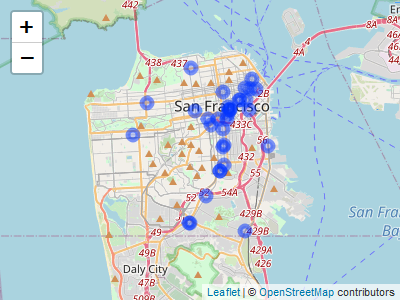
\includegraphics[width=0.9\linewidth]{crimebythenumbers_files/figure-latex/unnamed-chunk-10-1} \end{center}

Note that on the x-axis it prints out every single year and makes it completely unreadable. That is because the ``year'' column is a character type, so R thinks each year is its own category. It prints every single year because it thinks we want every category shown. To fix this we can make the column numeric and \texttt{ggplot()} will be smarter about printing fewer years.

\begin{Shaded}
\begin{Highlighting}[]
\NormalTok{penn\_alcohol}\SpecialCharTok{$}\NormalTok{year }\OtherTok{\textless{}{-}} \FunctionTok{as.numeric}\NormalTok{(penn\_alcohol}\SpecialCharTok{$}\NormalTok{year)}
\end{Highlighting}
\end{Shaded}

\begin{Shaded}
\begin{Highlighting}[]
\FunctionTok{ggplot}\NormalTok{(penn\_alcohol, }\FunctionTok{aes}\NormalTok{(}\AttributeTok{x =}\NormalTok{ year,}
                         \AttributeTok{y =}\NormalTok{ number\_of\_beers))}
\end{Highlighting}
\end{Shaded}

\begin{center}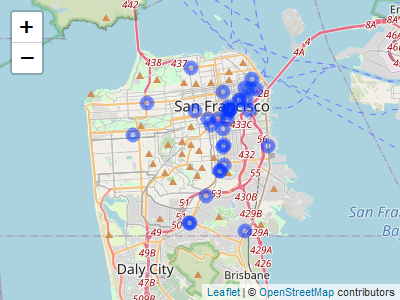
\includegraphics[width=0.9\linewidth]{crimebythenumbers_files/figure-latex/unnamed-chunk-12-1} \end{center}

When we run it, we get our graph. It includes the variable names for each axis and shows the range of data through the tick marks. What is missing is the actual data. For that we need to specify what type of graph it is. We literally add it with the + followed by the type of graph we want. Make sure that the + is at the end of a line, not the start of one. Starting a line with the + will not work.

Let's start with point and line graphs.

\begin{Shaded}
\begin{Highlighting}[]
\FunctionTok{ggplot}\NormalTok{(penn\_alcohol, }\FunctionTok{aes}\NormalTok{(}\AttributeTok{x =}\NormalTok{ year, }\AttributeTok{y =}\NormalTok{ number\_of\_beers)) }\SpecialCharTok{+}
  \FunctionTok{geom\_point}\NormalTok{()}
\end{Highlighting}
\end{Shaded}

\begin{center}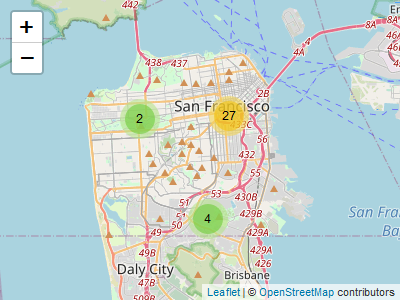
\includegraphics[width=0.9\linewidth]{crimebythenumbers_files/figure-latex/unnamed-chunk-13-1} \end{center}

\begin{Shaded}
\begin{Highlighting}[]
\FunctionTok{ggplot}\NormalTok{(penn\_alcohol, }\FunctionTok{aes}\NormalTok{(}\AttributeTok{x =}\NormalTok{ year, }\AttributeTok{y =}\NormalTok{ number\_of\_beers)) }\SpecialCharTok{+}
  \FunctionTok{geom\_line}\NormalTok{()}
\end{Highlighting}
\end{Shaded}

\begin{center}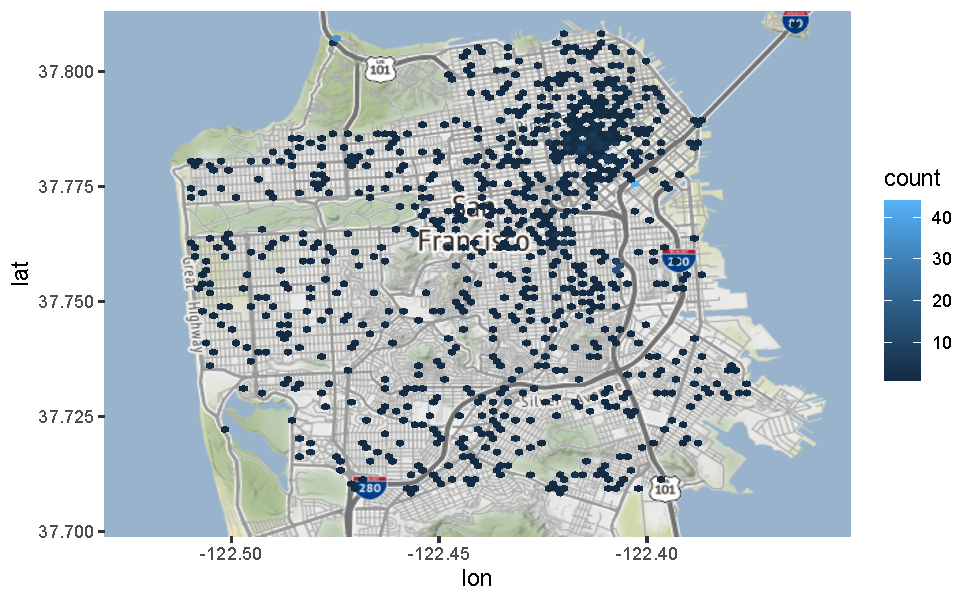
\includegraphics[width=0.9\linewidth]{crimebythenumbers_files/figure-latex/unnamed-chunk-14-1} \end{center}

We can also combine different types of graphs.

\begin{Shaded}
\begin{Highlighting}[]
\FunctionTok{ggplot}\NormalTok{(penn\_alcohol, }\FunctionTok{aes}\NormalTok{(}\AttributeTok{x =}\NormalTok{ year, }\AttributeTok{y =}\NormalTok{ number\_of\_beers)) }\SpecialCharTok{+}
  \FunctionTok{geom\_point}\NormalTok{() }\SpecialCharTok{+}
  \FunctionTok{geom\_line}\NormalTok{()}
\end{Highlighting}
\end{Shaded}

\begin{center}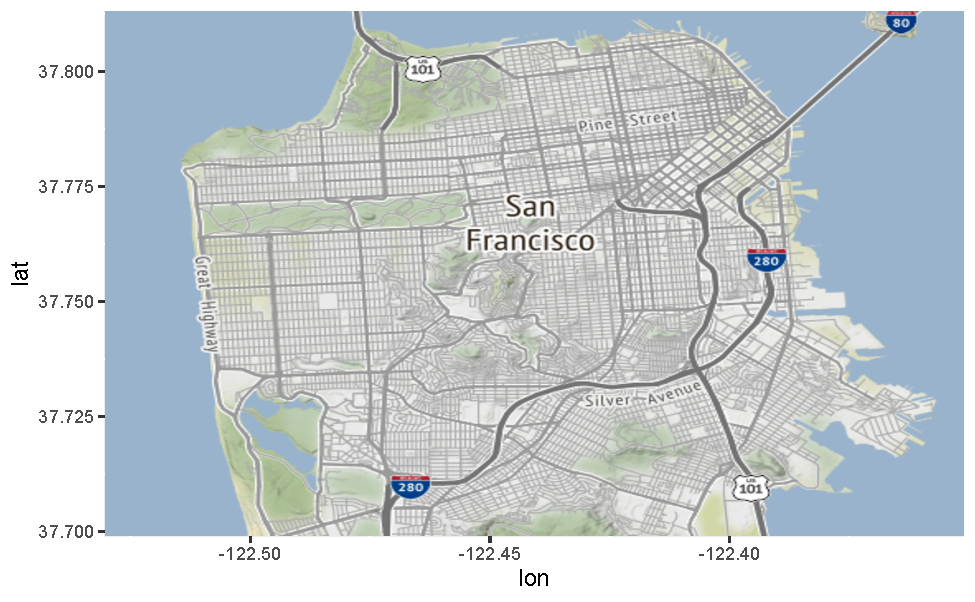
\includegraphics[width=0.9\linewidth]{crimebythenumbers_files/figure-latex/unnamed-chunk-15-1} \end{center}

It looks like there's a huge change in beer consumption over time. But look at where they y-axis starts. It starts around 280 so really that change is only \textasciitilde60 beers. That's because when graphs don't start at 0, it can make small changes appear big. We can fix this by forcing the y-axis to begin at 0. We can add \texttt{expand\_limits(y\ =\ 0)} to the graph to say that the value 0 must always appear on the y-axis, even if no data is close to that value.

\begin{Shaded}
\begin{Highlighting}[]
\FunctionTok{ggplot}\NormalTok{(penn\_alcohol, }\FunctionTok{aes}\NormalTok{(}\AttributeTok{x =}\NormalTok{ year, }\AttributeTok{y =}\NormalTok{ number\_of\_beers)) }\SpecialCharTok{+}
  \FunctionTok{geom\_point}\NormalTok{() }\SpecialCharTok{+}
  \FunctionTok{geom\_line}\NormalTok{() }\SpecialCharTok{+}
  \FunctionTok{expand\_limits}\NormalTok{(}\AttributeTok{y =} \DecValTok{0}\NormalTok{)}
\end{Highlighting}
\end{Shaded}

\begin{center}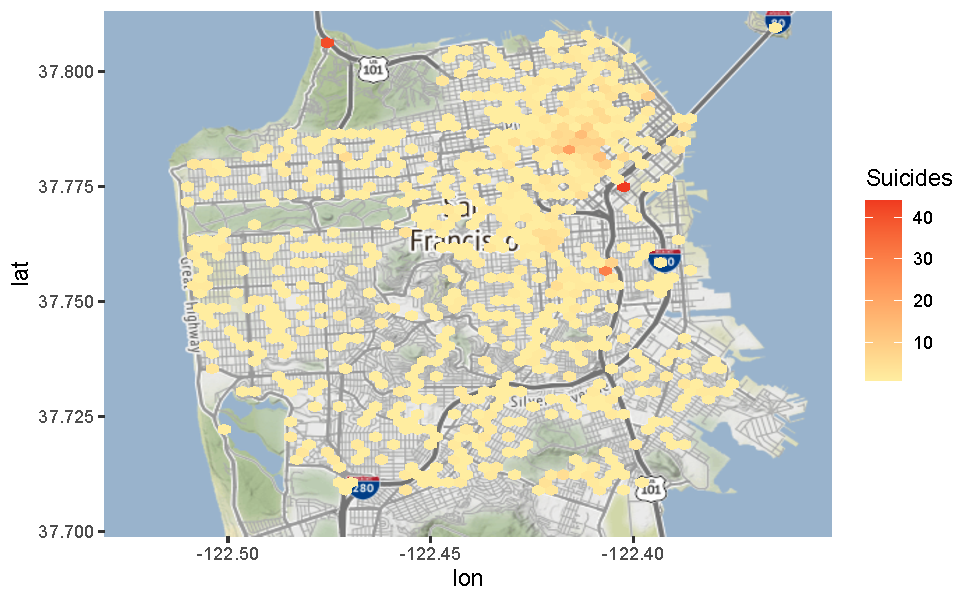
\includegraphics[width=0.9\linewidth]{crimebythenumbers_files/figure-latex/unnamed-chunk-16-1} \end{center}

Now that graph shows what looks like nearly no change even though that is also not true. Which graph is best? It's hard to say.

Inside the types of graphs we can change how it is displayed. As with using \texttt{plot()}, we can specify the color and size of our lines or points.

\begin{Shaded}
\begin{Highlighting}[]
\FunctionTok{ggplot}\NormalTok{(penn\_alcohol, }\FunctionTok{aes}\NormalTok{(}\AttributeTok{x =}\NormalTok{ year, }\AttributeTok{y =}\NormalTok{ number\_of\_beers)) }\SpecialCharTok{+}
  \FunctionTok{geom\_line}\NormalTok{(}\AttributeTok{color =} \StringTok{"forestgreen"}\NormalTok{, }\AttributeTok{size =} \FloatTok{1.3}\NormalTok{)}
\end{Highlighting}
\end{Shaded}

\begin{center}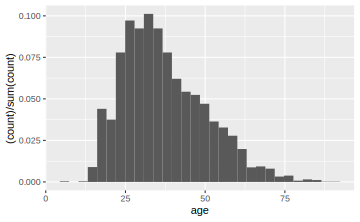
\includegraphics[width=0.9\linewidth]{crimebythenumbers_files/figure-latex/unnamed-chunk-17-1} \end{center}

Some other useful features are changing the axis labels and the graph title. Unlike in \texttt{plot()} we do not need to include it in the () of \texttt{ggplot()} but use their own functions to add them to the graph.

\begin{itemize}
\tightlist
\item
  \texttt{xlab()} - x-axis label
\item
  \texttt{ylab()} - y-axis label
\item
  \texttt{ggtitle()} - graph title
\end{itemize}

\begin{Shaded}
\begin{Highlighting}[]
\FunctionTok{ggplot}\NormalTok{(penn\_alcohol, }\FunctionTok{aes}\NormalTok{(}\AttributeTok{x =}\NormalTok{ year, }\AttributeTok{y =}\NormalTok{ number\_of\_beers)) }\SpecialCharTok{+}
  \FunctionTok{geom\_line}\NormalTok{(}\AttributeTok{color =} \StringTok{"forestgreen"}\NormalTok{, }\AttributeTok{size =} \FloatTok{1.3}\NormalTok{) }\SpecialCharTok{+}
  \FunctionTok{xlab}\NormalTok{(}\StringTok{"Year"}\NormalTok{) }\SpecialCharTok{+}
  \FunctionTok{ylab}\NormalTok{(}\StringTok{"Number of Beers"}\NormalTok{) }\SpecialCharTok{+}
  \FunctionTok{ggtitle}\NormalTok{(}\StringTok{"PA Annual Beer Consumption Per Capita (1977{-}2017)"}\NormalTok{)}
\end{Highlighting}
\end{Shaded}

\begin{center}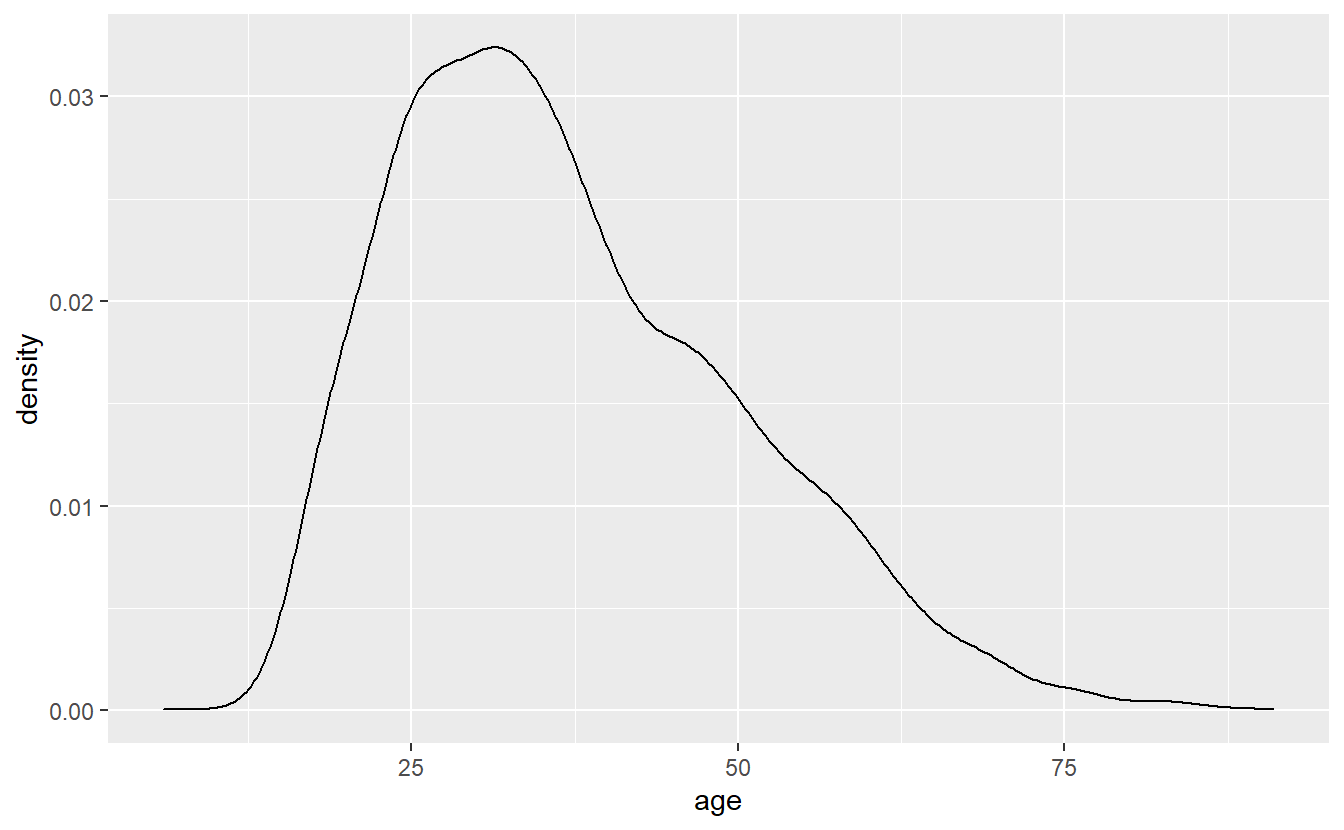
\includegraphics[width=0.9\linewidth]{crimebythenumbers_files/figure-latex/unnamed-chunk-18-1} \end{center}

Many time-series plots show multiple variables over the same time period (e.g.~murder and robbery over time). There are ways to change the data itself to make creating graphs like this easier, but let's stick with the data we currently have and just change \texttt{ggplot()}.

Start with a normal line graph, this time looking at wine.

\begin{Shaded}
\begin{Highlighting}[]
\FunctionTok{ggplot}\NormalTok{(penn\_alcohol, }\FunctionTok{aes}\NormalTok{(}\AttributeTok{x =}\NormalTok{ year, }\AttributeTok{y =}\NormalTok{ number\_of\_glasses\_wine)) }\SpecialCharTok{+}
  \FunctionTok{geom\_line}\NormalTok{()}
\end{Highlighting}
\end{Shaded}

\begin{center}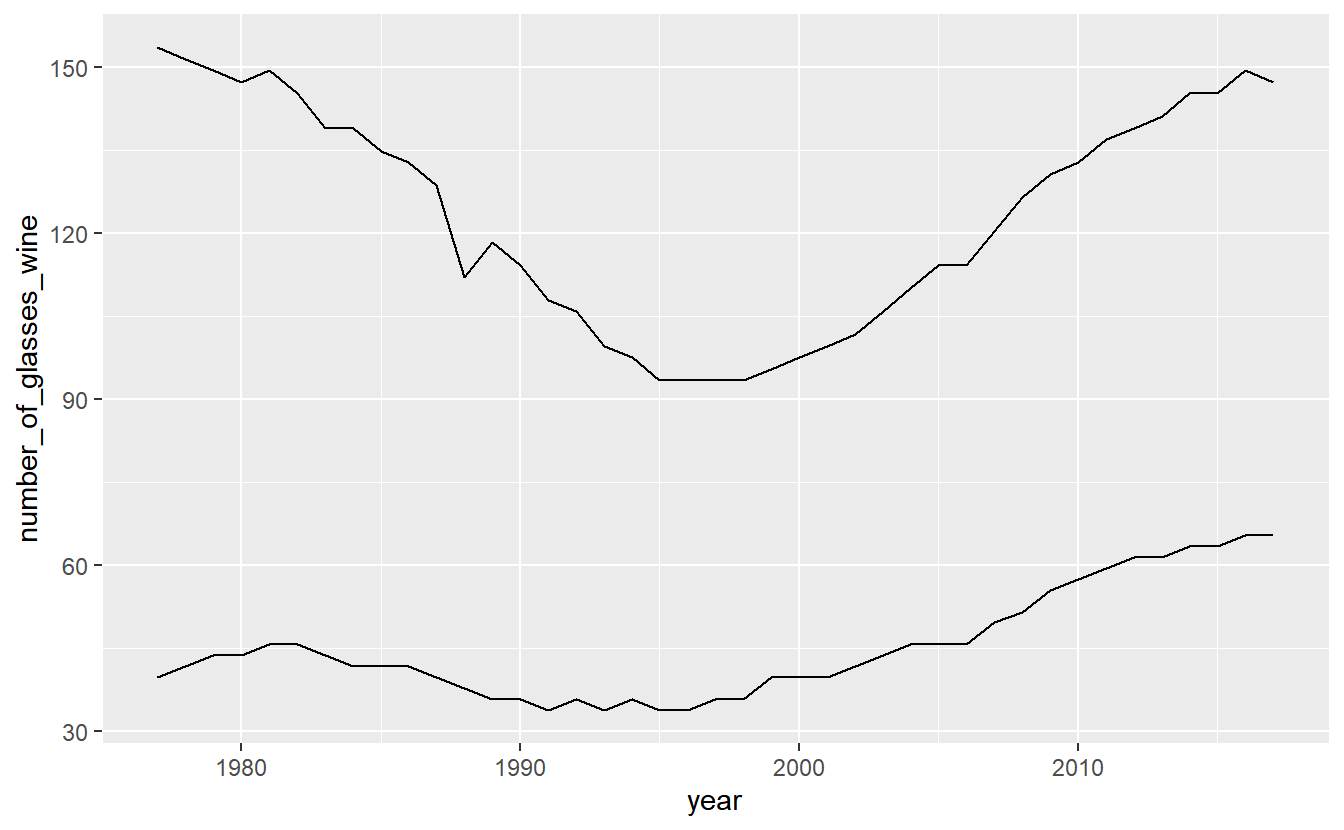
\includegraphics[width=0.9\linewidth]{crimebythenumbers_files/figure-latex/unnamed-chunk-19-1} \end{center}

Then include a second geom\_line() with its own aes() for the second variable.

\begin{Shaded}
\begin{Highlighting}[]
\FunctionTok{ggplot}\NormalTok{(penn\_alcohol, }\FunctionTok{aes}\NormalTok{(}\AttributeTok{x =}\NormalTok{ year, }\AttributeTok{y =}\NormalTok{ number\_of\_glasses\_wine)) }\SpecialCharTok{+}
  \FunctionTok{geom\_line}\NormalTok{() }\SpecialCharTok{+}
  \FunctionTok{geom\_line}\NormalTok{(}\FunctionTok{aes}\NormalTok{(}\AttributeTok{x =}\NormalTok{ year, }\AttributeTok{y =}\NormalTok{ number\_of\_shots\_liquor))}
\end{Highlighting}
\end{Shaded}

\begin{center}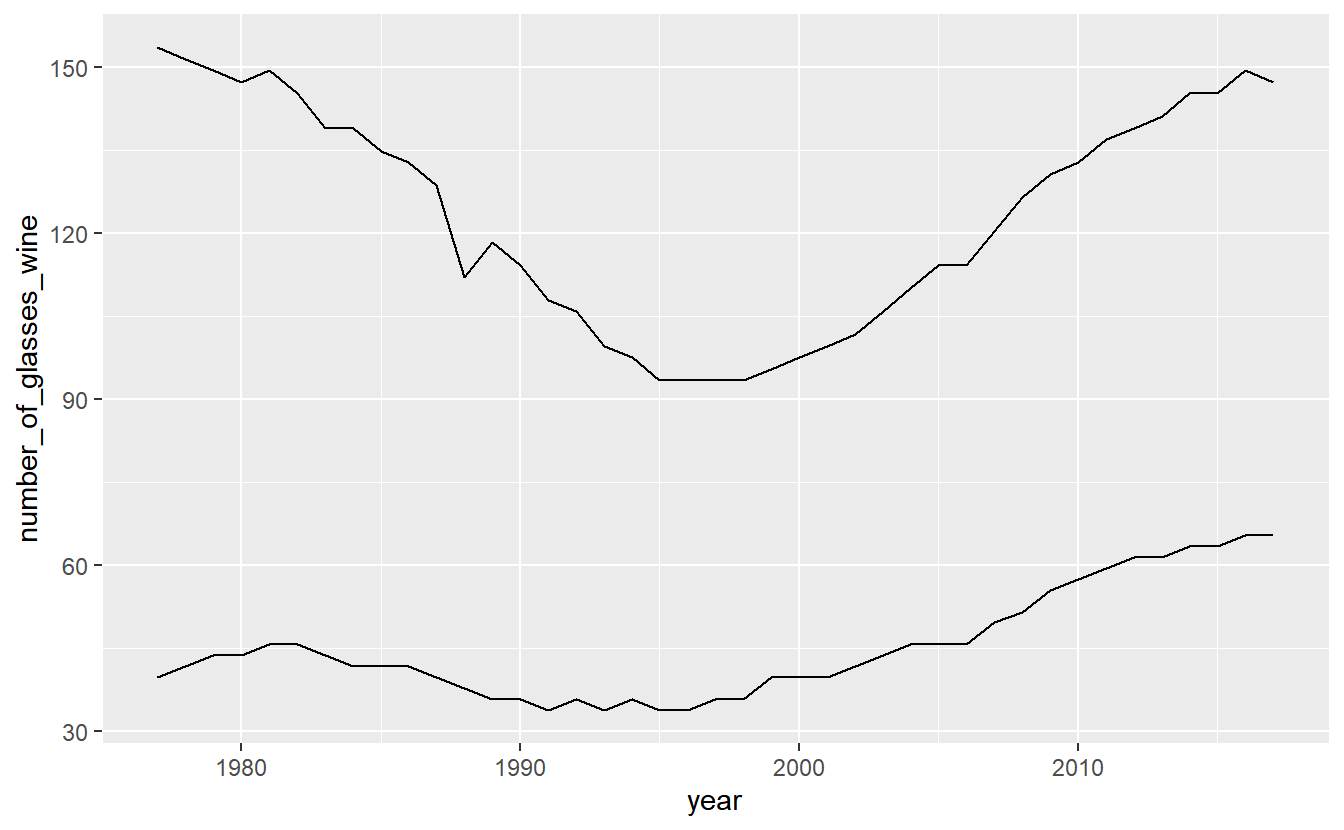
\includegraphics[width=0.9\linewidth]{crimebythenumbers_files/figure-latex/unnamed-chunk-20-1} \end{center}

A problem with this is that both lines are the same color. We need to set a color for each line and do so within \texttt{aes()}. Instead of providing a color name, we need to provide the name the color will have in the legend. Do so for both lines.

\begin{Shaded}
\begin{Highlighting}[]
\FunctionTok{ggplot}\NormalTok{(penn\_alcohol, }\FunctionTok{aes}\NormalTok{(}\AttributeTok{x =}\NormalTok{ year, }\AttributeTok{y =}\NormalTok{ number\_of\_glasses\_wine,}
                         \AttributeTok{color =} \StringTok{"Glasses of Wine"}\NormalTok{)) }\SpecialCharTok{+}
  \FunctionTok{geom\_line}\NormalTok{() }\SpecialCharTok{+}
  \FunctionTok{geom\_line}\NormalTok{(}\FunctionTok{aes}\NormalTok{(}\AttributeTok{x =}\NormalTok{ year, }\AttributeTok{y =}\NormalTok{ number\_of\_shots\_liquor,}
                \AttributeTok{color =} \StringTok{"Shots of Liquor"}\NormalTok{))}
\end{Highlighting}
\end{Shaded}

\begin{center}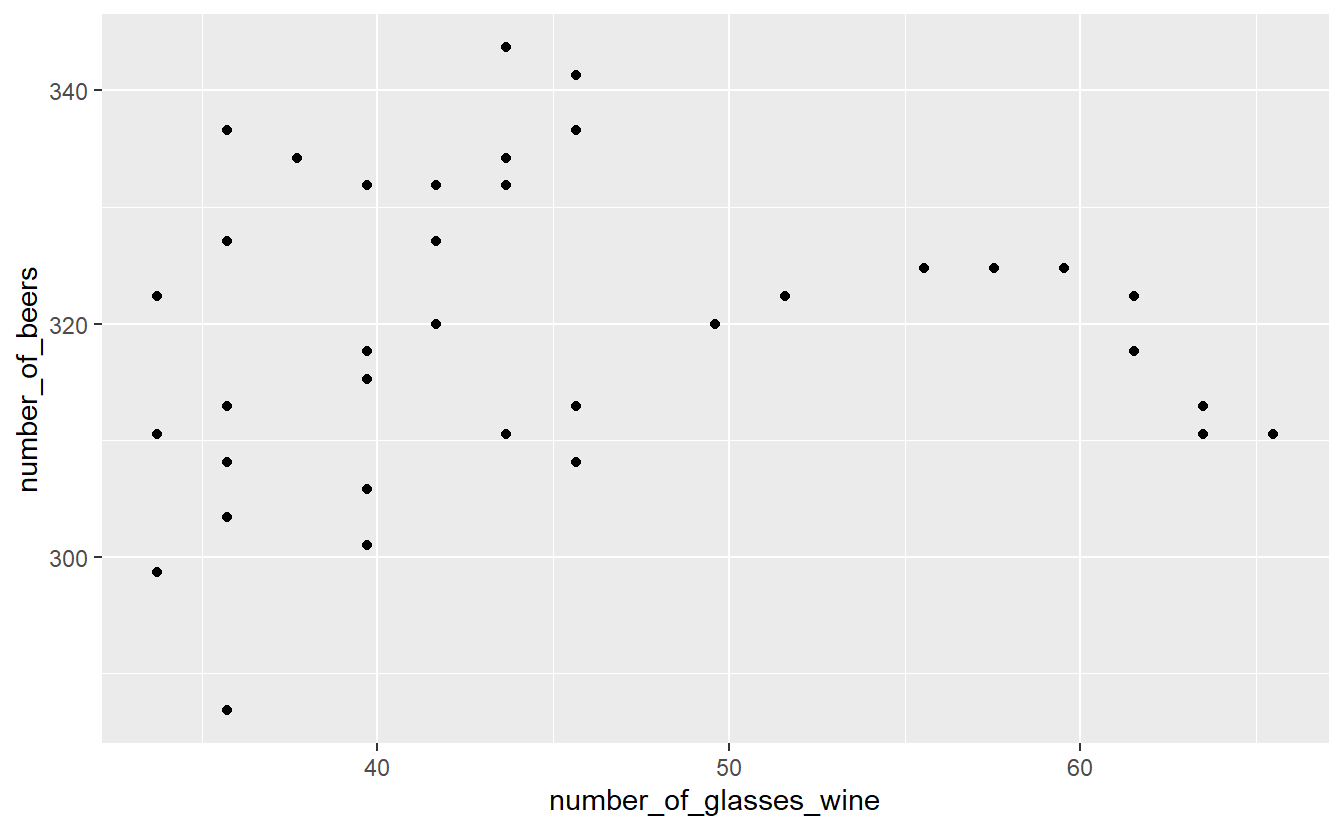
\includegraphics[width=0.9\linewidth]{crimebythenumbers_files/figure-latex/unnamed-chunk-21-1} \end{center}

We can change the legend title by using the function \texttt{labs()} and changing the value \texttt{color} to what we want the legend title to be.

\begin{Shaded}
\begin{Highlighting}[]
\FunctionTok{ggplot}\NormalTok{(penn\_alcohol, }\FunctionTok{aes}\NormalTok{(}\AttributeTok{x =}\NormalTok{ year, }\AttributeTok{y =}\NormalTok{ number\_of\_glasses\_wine,}
                         \AttributeTok{color =} \StringTok{"Glasses of Wine"}\NormalTok{)) }\SpecialCharTok{+}
  \FunctionTok{geom\_line}\NormalTok{() }\SpecialCharTok{+}
  \FunctionTok{geom\_line}\NormalTok{(}\FunctionTok{aes}\NormalTok{(}\AttributeTok{x =}\NormalTok{ year, }\AttributeTok{y =}\NormalTok{ number\_of\_shots\_liquor,}
                \AttributeTok{color =} \StringTok{"Shots of Liquor"}\NormalTok{)) }\SpecialCharTok{+}
  \FunctionTok{labs}\NormalTok{(}\AttributeTok{color =} \StringTok{"Alcohol Type"}\NormalTok{)}
\end{Highlighting}
\end{Shaded}

\begin{center}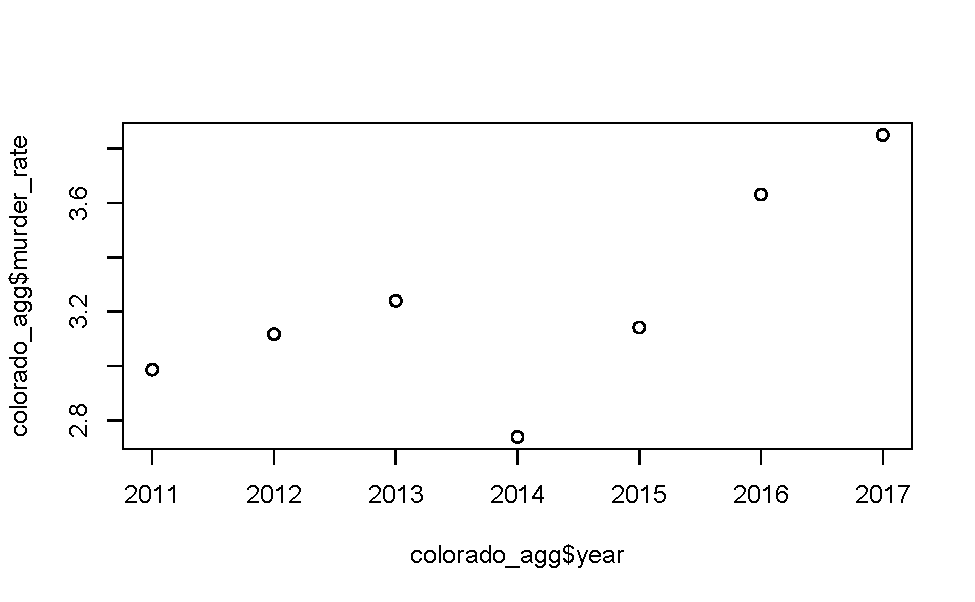
\includegraphics[width=0.9\linewidth]{crimebythenumbers_files/figure-latex/unnamed-chunk-22-1} \end{center}

Finally, a useful option to move the legend from the side to the bottom is setting the \texttt{theme()} function to move the \texttt{legend.position} to ``bottom''. This will allow the graph to be wider.

\begin{Shaded}
\begin{Highlighting}[]
\FunctionTok{ggplot}\NormalTok{(penn\_alcohol, }\FunctionTok{aes}\NormalTok{(}\AttributeTok{x =}\NormalTok{ year, }\AttributeTok{y =}\NormalTok{ number\_of\_glasses\_wine,}
                         \AttributeTok{color =} \StringTok{"Glasses of Wine"}\NormalTok{)) }\SpecialCharTok{+}
  \FunctionTok{geom\_line}\NormalTok{() }\SpecialCharTok{+}
  \FunctionTok{geom\_line}\NormalTok{(}\FunctionTok{aes}\NormalTok{(}\AttributeTok{x =}\NormalTok{ year, }\AttributeTok{y =}\NormalTok{ number\_of\_shots\_liquor,}
                \AttributeTok{color =} \StringTok{"Shots of Liquor"}\NormalTok{)) }\SpecialCharTok{+}
  \FunctionTok{labs}\NormalTok{(}\AttributeTok{color =} \StringTok{"Alcohol Type"}\NormalTok{) }\SpecialCharTok{+}
  \FunctionTok{theme}\NormalTok{(}\AttributeTok{legend.position =} \StringTok{"bottom"}\NormalTok{)}
\end{Highlighting}
\end{Shaded}

\begin{center}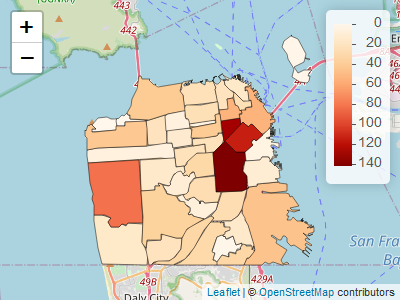
\includegraphics[width=0.9\linewidth]{crimebythenumbers_files/figure-latex/unnamed-chunk-23-1} \end{center}

\hypertarget{scatter-plots}{%
\section{Scatter Plots}\label{scatter-plots}}

Making a scatter plot simply requires changing the x-axis from year to another numerical variable and using geom\_point().

\begin{Shaded}
\begin{Highlighting}[]
\FunctionTok{ggplot}\NormalTok{(penn\_alcohol, }\FunctionTok{aes}\NormalTok{(}\AttributeTok{x =}\NormalTok{ number\_of\_shots\_liquor,}
                         \AttributeTok{y =}\NormalTok{ number\_of\_beers)) }\SpecialCharTok{+}
  \FunctionTok{geom\_point}\NormalTok{()}
\end{Highlighting}
\end{Shaded}

\begin{center}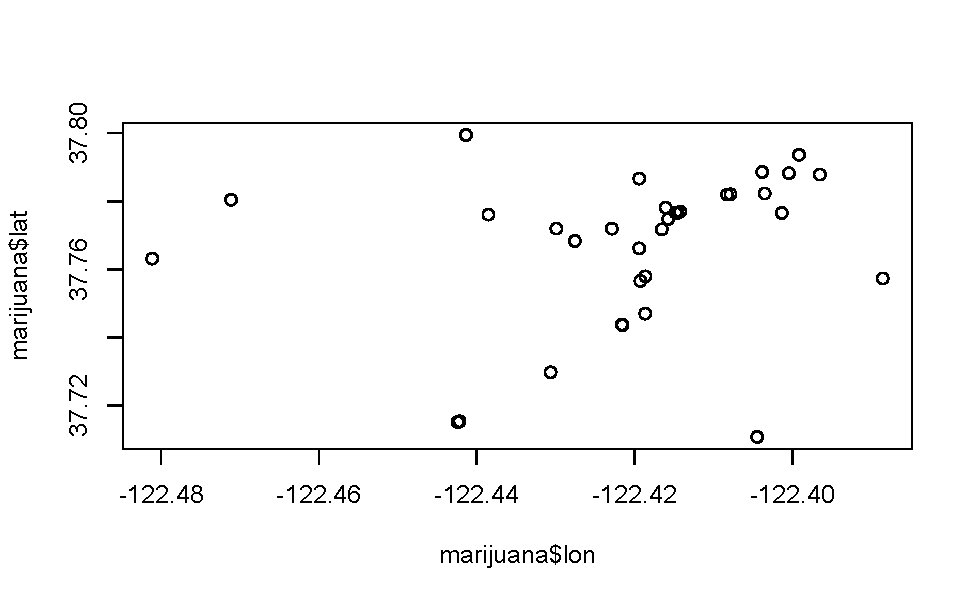
\includegraphics[width=0.9\linewidth]{crimebythenumbers_files/figure-latex/unnamed-chunk-24-1} \end{center}

This graph shows us that when liquor consumption increases, beer consumption also tends to increase.

While scatterplots can help show the relationship between variables, we lose the information of how consumption changes over time.

\hypertarget{color-blindness}{%
\section{Color blindness}\label{color-blindness}}

Please keep in mind that some people are color blind so graphs (or maps which we will learn about soon) will be hard to read for these people if we choose the incorrect colors. A helpful site for choosing colors for graphs is \href{http://colorbrewer2.org}{colorbrewer2.org}

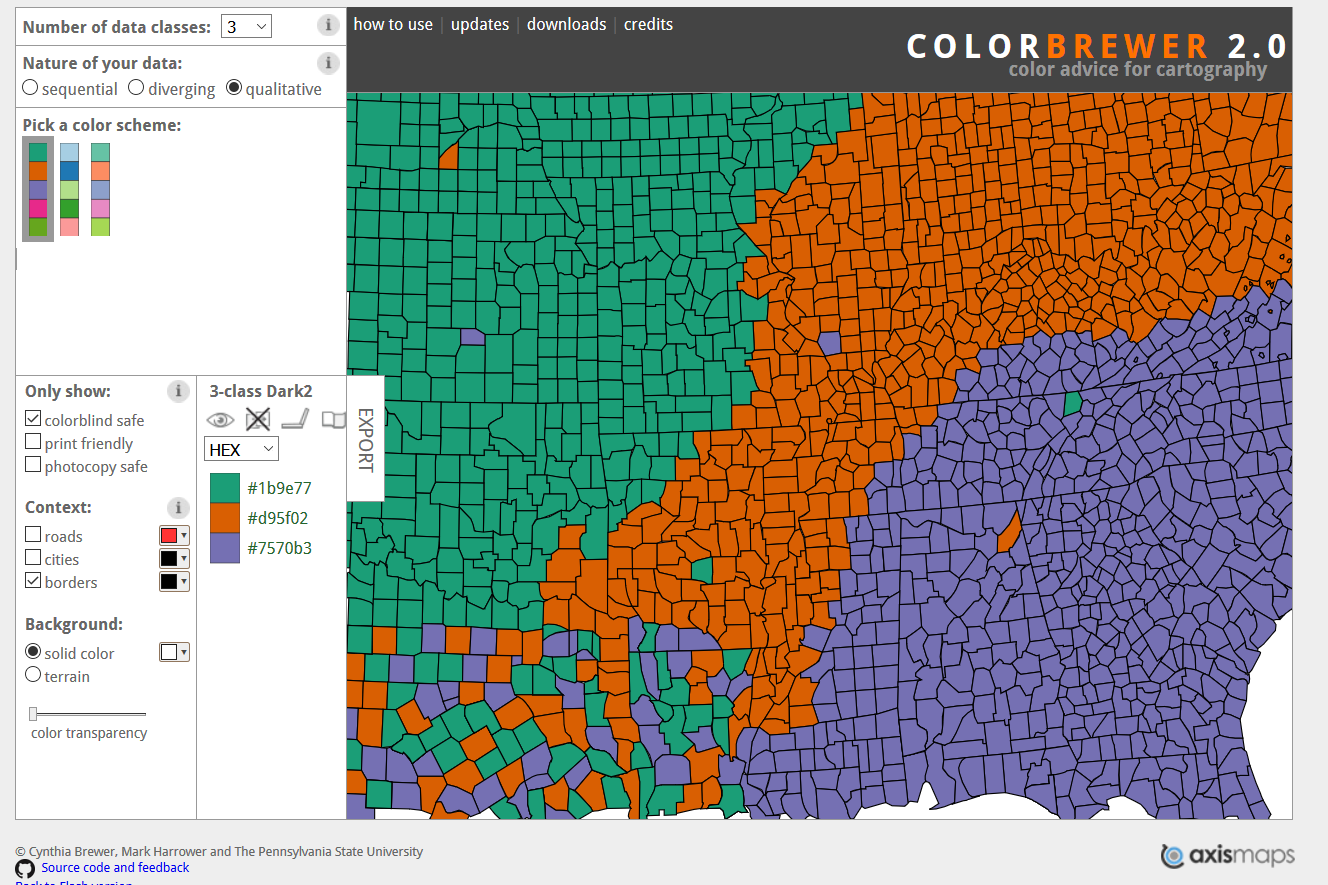
\includegraphics{images/colorbrewer.PNG}

This site lets you select which type of colors you want (sequential and diverging such as shades in a hotspot map, and qualitative such as for data like what we used in this lesson). In the ``Only show:'' section you can set it to ``colorblind safe'' to restrict it to colors that allow people with color blindness to read your graph. To the right of this section it shows the HEX codes for each color (a HEX code is just a code that a computer can read and know exactly which color it is).

Let's use an example of a color blind friendly color from the ``qualitative'' section of ColorBrewer. We have three options on this page (we can change how many colors we want but it defaults to showing 3): green (HEX = \#1b9e77), orange (HEX = \#d95f02), and purple (HEX = \#7570b3). We'll use the orange and purple colors. To manually set colors in \texttt{ggplot()} we use \texttt{scale\_color\_manual(values\ =\ c())} and include a vector of color names or HEX codes inside the \texttt{c()}. Doing that using the orange and purple HEX codes will change our graph colors to these two colors.

\begin{Shaded}
\begin{Highlighting}[]
\FunctionTok{ggplot}\NormalTok{(penn\_alcohol, }\FunctionTok{aes}\NormalTok{(}\AttributeTok{x =}\NormalTok{ year, }\AttributeTok{y =}\NormalTok{ number\_of\_glasses\_wine,}
                         \AttributeTok{color =} \StringTok{"Glasses of Wine"}\NormalTok{)) }\SpecialCharTok{+}
  \FunctionTok{geom\_line}\NormalTok{() }\SpecialCharTok{+}
  \FunctionTok{geom\_line}\NormalTok{(}\FunctionTok{aes}\NormalTok{(}\AttributeTok{x =}\NormalTok{ year, }\AttributeTok{y =}\NormalTok{ number\_of\_shots\_liquor,}
                \AttributeTok{color =} \StringTok{"number\_of\_shots\_liquor"}\NormalTok{)) }\SpecialCharTok{+}
  \FunctionTok{labs}\NormalTok{(}\AttributeTok{color =} \StringTok{"Alcohol Type"}\NormalTok{) }\SpecialCharTok{+}
  \FunctionTok{theme}\NormalTok{(}\AttributeTok{legend.position =} \StringTok{"bottom"}\NormalTok{) }\SpecialCharTok{+}
  \FunctionTok{scale\_color\_manual}\NormalTok{(}\AttributeTok{values =} \FunctionTok{c}\NormalTok{(}\StringTok{"\#7570b3"}\NormalTok{, }\StringTok{"\#d95f02"}\NormalTok{))}
\end{Highlighting}
\end{Shaded}

\begin{center}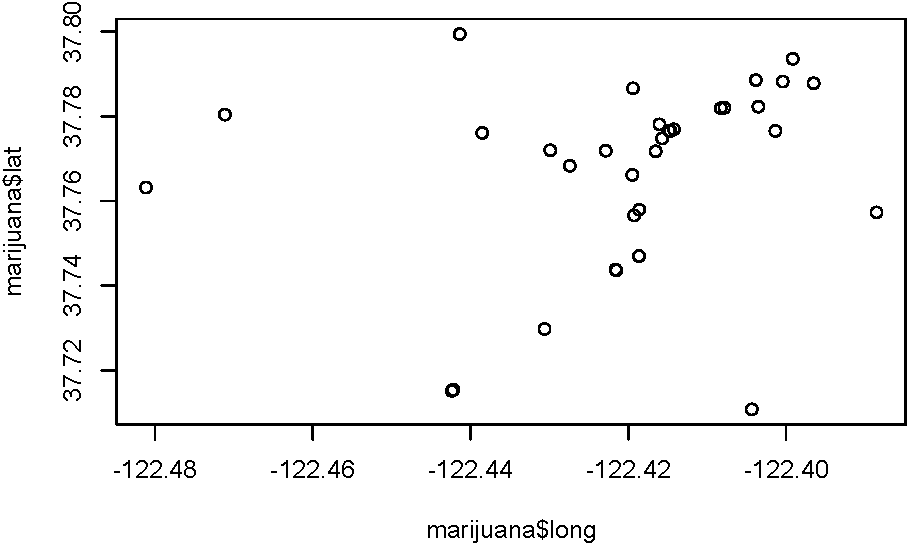
\includegraphics[width=0.9\linewidth]{crimebythenumbers_files/figure-latex/unnamed-chunk-25-1} \end{center}

\hypertarget{ois_graphs}{%
\chapter{\texorpdfstring{More graphing with \texttt{ggplot2}}{More graphing with ggplot2}}\label{ois_graphs}}

In this lesson we will continue to explore graphing using \texttt{ggplot()}. The data we will use is a database of officer-involved shootings that result in a death in the United States since January 1st, 2015. This data has been compiled and released by the Washington Post so it will be a useful exercise in exploring data from non-government sources. This data is useful for our purposes as it has a number of variables related to the person who was shot, allowing us to practice making many types of graphs.
To explore the data on their website, see \href{https://www.washingtonpost.com/graphics/2019/national/police-shootings-2019/?utm_term=.e870afc9a00c}{here}.
To examine their methodology, see \href{https://www.washingtonpost.com/national/how-the-washington-post-is-examining-police-shootings-in-the-united-states/2016/07/07/d9c52238-43ad-11e6-8856-f26de2537a9d_story.html?utm_term=.f07e9800092b}{here}.

The data initially comes as a .csv file so we'll use the \texttt{read\_csv()} function from the \texttt{readr} package. Since it's available on GitHub, we can download it by directing \texttt{read\_csv()} to read the file at its URL on GitHub.

\begin{Shaded}
\begin{Highlighting}[]
\FunctionTok{library}\NormalTok{(readr)}
\NormalTok{shootings }\OtherTok{\textless{}{-}} \FunctionTok{read\_csv}\NormalTok{(}\StringTok{"https://raw.githubusercontent.com/washingtonpost/data{-}police{-}shootings/master/fatal{-}police{-}shootings{-}data.csv"}\NormalTok{)}
\CommentTok{\#\textgreater{} }
\CommentTok{\#\textgreater{} {-}{-} Column specification {-}{-}{-}{-}{-}{-}{-}{-}{-}{-}{-}{-}{-}{-}{-}{-}{-}{-}{-}{-}{-}{-}{-}{-}{-}{-}{-}{-}{-}{-}{-}{-}}
\CommentTok{\#\textgreater{} cols(}
\CommentTok{\#\textgreater{}   id = col\_double(),}
\CommentTok{\#\textgreater{}   name = col\_character(),}
\CommentTok{\#\textgreater{}   date = col\_date(format = ""),}
\CommentTok{\#\textgreater{}   manner\_of\_death = col\_character(),}
\CommentTok{\#\textgreater{}   armed = col\_character(),}
\CommentTok{\#\textgreater{}   age = col\_double(),}
\CommentTok{\#\textgreater{}   gender = col\_character(),}
\CommentTok{\#\textgreater{}   race = col\_character(),}
\CommentTok{\#\textgreater{}   city = col\_character(),}
\CommentTok{\#\textgreater{}   state = col\_character(),}
\CommentTok{\#\textgreater{}   signs\_of\_mental\_illness = col\_logical(),}
\CommentTok{\#\textgreater{}   threat\_level = col\_character(),}
\CommentTok{\#\textgreater{}   flee = col\_character(),}
\CommentTok{\#\textgreater{}   body\_camera = col\_logical(),}
\CommentTok{\#\textgreater{}   longitude = col\_double(),}
\CommentTok{\#\textgreater{}   latitude = col\_double(),}
\CommentTok{\#\textgreater{}   is\_geocoding\_exact = col\_logical()}
\CommentTok{\#\textgreater{} )}
\end{Highlighting}
\end{Shaded}

Since \texttt{read\_csv()} reads files into a tibble object, we'll turn it into a data.frame so \texttt{head()} shows every single column.

\begin{Shaded}
\begin{Highlighting}[]
\NormalTok{shootings }\OtherTok{\textless{}{-}} \FunctionTok{as.data.frame}\NormalTok{(shootings)}
\end{Highlighting}
\end{Shaded}

\hypertarget{exploring-data}{%
\section{Exploring Data}\label{exploring-data}}

Now that we have the data read in, let's look at it.

\begin{Shaded}
\begin{Highlighting}[]
\FunctionTok{nrow}\NormalTok{(shootings)}
\CommentTok{\#\textgreater{} [1] 6223}
\FunctionTok{ncol}\NormalTok{(shootings)}
\CommentTok{\#\textgreater{} [1] 17}
\end{Highlighting}
\end{Shaded}

The data has 17 variables and covers 6223 shootings. Let's check out some of the variables, first using \texttt{head()} then using \texttt{summary()} and \texttt{table()}.

\begin{Shaded}
\begin{Highlighting}[]
\FunctionTok{head}\NormalTok{(shootings)}
\CommentTok{\#\textgreater{}   id               name       date  manner\_of\_death}
\CommentTok{\#\textgreater{} 1  3         Tim Elliot 2015{-}01{-}02             shot}
\CommentTok{\#\textgreater{} 2  4   Lewis Lee Lembke 2015{-}01{-}02             shot}
\CommentTok{\#\textgreater{} 3  5 John Paul Quintero 2015{-}01{-}03 shot and Tasered}
\CommentTok{\#\textgreater{} 4  8    Matthew Hoffman 2015{-}01{-}04             shot}
\CommentTok{\#\textgreater{} 5  9  Michael Rodriguez 2015{-}01{-}04             shot}
\CommentTok{\#\textgreater{} 6 11  Kenneth Joe Brown 2015{-}01{-}04             shot}
\CommentTok{\#\textgreater{}        armed age gender race          city state}
\CommentTok{\#\textgreater{} 1        gun  53      M    A       Shelton    WA}
\CommentTok{\#\textgreater{} 2        gun  47      M    W         Aloha    OR}
\CommentTok{\#\textgreater{} 3    unarmed  23      M    H       Wichita    KS}
\CommentTok{\#\textgreater{} 4 toy weapon  32      M    W San Francisco    CA}
\CommentTok{\#\textgreater{} 5   nail gun  39      M    H         Evans    CO}
\CommentTok{\#\textgreater{} 6        gun  18      M    W       Guthrie    OK}
\CommentTok{\#\textgreater{}   signs\_of\_mental\_illness threat\_level        flee}
\CommentTok{\#\textgreater{} 1                    TRUE       attack Not fleeing}
\CommentTok{\#\textgreater{} 2                   FALSE       attack Not fleeing}
\CommentTok{\#\textgreater{} 3                   FALSE        other Not fleeing}
\CommentTok{\#\textgreater{} 4                    TRUE       attack Not fleeing}
\CommentTok{\#\textgreater{} 5                   FALSE       attack Not fleeing}
\CommentTok{\#\textgreater{} 6                   FALSE       attack Not fleeing}
\CommentTok{\#\textgreater{}   body\_camera longitude latitude is\_geocoding\_exact}
\CommentTok{\#\textgreater{} 1       FALSE  {-}123.122   47.247               TRUE}
\CommentTok{\#\textgreater{} 2       FALSE  {-}122.892   45.487               TRUE}
\CommentTok{\#\textgreater{} 3       FALSE   {-}97.281   37.695               TRUE}
\CommentTok{\#\textgreater{} 4       FALSE  {-}122.422   37.763               TRUE}
\CommentTok{\#\textgreater{} 5       FALSE  {-}104.692   40.384               TRUE}
\CommentTok{\#\textgreater{} 6       FALSE   {-}97.423   35.877               TRUE}
\end{Highlighting}
\end{Shaded}

Each row is a single shooting and it includes variables such as the victim's name, the date of the shooting, demographic information about that person, the city and state where the shooting occurred, and some information about the incident. It is clear from these first 6 rows that most variables are categorical so we can't use \texttt{summary()} on them. Let's use \texttt{summary()} on the date and age columns and then use \texttt{table()} for the rest.

\begin{Shaded}
\begin{Highlighting}[]
\FunctionTok{summary}\NormalTok{(shootings}\SpecialCharTok{$}\NormalTok{date)}
\CommentTok{\#\textgreater{}         Min.      1st Qu.       Median         Mean }
\CommentTok{\#\textgreater{} "2015{-}01{-}02" "2016{-}07{-}28" "2018{-}02{-}26" "2018{-}02{-}24" }
\CommentTok{\#\textgreater{}      3rd Qu.         Max. }
\CommentTok{\#\textgreater{} "2019{-}10{-}06" "2021{-}04{-}18"}
\FunctionTok{summary}\NormalTok{(shootings}\SpecialCharTok{$}\NormalTok{age)}
\CommentTok{\#\textgreater{}    Min. 1st Qu.  Median    Mean 3rd Qu.    Max.    NA\textquotesingle{}s }
\CommentTok{\#\textgreater{}    6.00   27.00   35.00   37.11   46.00   91.00     280}
\end{Highlighting}
\end{Shaded}

From this we can see that the data is from early January through about a week ago. From the age column we can see that the average age is about 37 with most people around that range. Now we can use \texttt{table()} to see how often each value appears in each variable. We don't want to do this for city or name as there would be too many values, but it will work for the other columns. Let's start with the ``manner\_of\_death'' column.

\begin{Shaded}
\begin{Highlighting}[]
\FunctionTok{table}\NormalTok{(shootings}\SpecialCharTok{$}\NormalTok{manner\_of\_death)}
\CommentTok{\#\textgreater{} }
\CommentTok{\#\textgreater{}             shot shot and Tasered }
\CommentTok{\#\textgreater{}             5906              317}
\end{Highlighting}
\end{Shaded}

To turn these counts into percentages we can divide the results by the number of rows in our data and multiply by 100.

\begin{Shaded}
\begin{Highlighting}[]
\FunctionTok{table}\NormalTok{(shootings}\SpecialCharTok{$}\NormalTok{manner\_of\_death) }\SpecialCharTok{/} \FunctionTok{nrow}\NormalTok{(shootings) }\SpecialCharTok{*} \DecValTok{100}
\CommentTok{\#\textgreater{} }
\CommentTok{\#\textgreater{}             shot shot and Tasered }
\CommentTok{\#\textgreater{}        94.905994         5.094006}
\end{Highlighting}
\end{Shaded}

Now it is clear to see that in about 95\% of shootings, officers used a gun and in 5\% of shootings they also used a Taser. As this is data on officer shooting deaths, this is unsurprising. Let's take a look at whether the victim was armed.

\begin{Shaded}
\begin{Highlighting}[]
\FunctionTok{table}\NormalTok{(shootings}\SpecialCharTok{$}\NormalTok{armed) }\SpecialCharTok{/} \FunctionTok{nrow}\NormalTok{(shootings) }\SpecialCharTok{*} \DecValTok{100}
\CommentTok{\#\textgreater{} }
\CommentTok{\#\textgreater{}                  air conditioner }
\CommentTok{\#\textgreater{}                       0.01606942 }
\CommentTok{\#\textgreater{}                       air pistol }
\CommentTok{\#\textgreater{}                       0.01606942 }
\CommentTok{\#\textgreater{}                   Airsoft pistol }
\CommentTok{\#\textgreater{}                       0.04820826 }
\CommentTok{\#\textgreater{}                               ax }
\CommentTok{\#\textgreater{}                       0.38566608 }
\CommentTok{\#\textgreater{}                         barstool }
\CommentTok{\#\textgreater{}                       0.01606942 }
\CommentTok{\#\textgreater{}                     baseball bat }
\CommentTok{\#\textgreater{}                       0.32138840 }
\CommentTok{\#\textgreater{}          baseball bat and bottle }
\CommentTok{\#\textgreater{}                       0.01606942 }
\CommentTok{\#\textgreater{} baseball bat and fireplace poker }
\CommentTok{\#\textgreater{}                       0.01606942 }
\CommentTok{\#\textgreater{}           baseball bat and knife }
\CommentTok{\#\textgreater{}                       0.01606942 }
\CommentTok{\#\textgreater{}                            baton }
\CommentTok{\#\textgreater{}                       0.09641652 }
\CommentTok{\#\textgreater{}                          bayonet }
\CommentTok{\#\textgreater{}                       0.01606942 }
\CommentTok{\#\textgreater{}                           BB gun }
\CommentTok{\#\textgreater{}                       0.17676362 }
\CommentTok{\#\textgreater{}               BB gun and vehicle }
\CommentTok{\#\textgreater{}                       0.01606942 }
\CommentTok{\#\textgreater{}                     bean{-}bag gun }
\CommentTok{\#\textgreater{}                       0.01606942 }
\CommentTok{\#\textgreater{}                      beer bottle }
\CommentTok{\#\textgreater{}                       0.04820826 }
\CommentTok{\#\textgreater{}                       binoculars }
\CommentTok{\#\textgreater{}                       0.01606942 }
\CommentTok{\#\textgreater{}                     blunt object }
\CommentTok{\#\textgreater{}                       0.08034710 }
\CommentTok{\#\textgreater{}                           bottle }
\CommentTok{\#\textgreater{}                       0.01606942 }
\CommentTok{\#\textgreater{}                    bow and arrow }
\CommentTok{\#\textgreater{}                       0.01606942 }
\CommentTok{\#\textgreater{}                       box cutter }
\CommentTok{\#\textgreater{}                       0.20890246 }
\CommentTok{\#\textgreater{}                            brick }
\CommentTok{\#\textgreater{}                       0.03213884 }
\CommentTok{\#\textgreater{}              car, knife and mace }
\CommentTok{\#\textgreater{}                       0.01606942 }
\CommentTok{\#\textgreater{}                          carjack }
\CommentTok{\#\textgreater{}                       0.01606942 }
\CommentTok{\#\textgreater{}                            chain }
\CommentTok{\#\textgreater{}                       0.04820826 }
\CommentTok{\#\textgreater{}                        chain saw }
\CommentTok{\#\textgreater{}                       0.03213884 }
\CommentTok{\#\textgreater{}                         chainsaw }
\CommentTok{\#\textgreater{}                       0.01606942 }
\CommentTok{\#\textgreater{}                            chair }
\CommentTok{\#\textgreater{}                       0.06427768 }
\CommentTok{\#\textgreater{}              claimed to be armed }
\CommentTok{\#\textgreater{}                       0.01606942 }
\CommentTok{\#\textgreater{}               contractor\textquotesingle{}s level }
\CommentTok{\#\textgreater{}                       0.01606942 }
\CommentTok{\#\textgreater{}                   cordless drill }
\CommentTok{\#\textgreater{}                       0.01606942 }
\CommentTok{\#\textgreater{}                         crossbow }
\CommentTok{\#\textgreater{}                       0.14462478 }
\CommentTok{\#\textgreater{}                          crowbar }
\CommentTok{\#\textgreater{}                       0.06427768 }
\CommentTok{\#\textgreater{}                        fireworks }
\CommentTok{\#\textgreater{}                       0.01606942 }
\CommentTok{\#\textgreater{}                         flagpole }
\CommentTok{\#\textgreater{}                       0.01606942 }
\CommentTok{\#\textgreater{}                       flashlight }
\CommentTok{\#\textgreater{}                       0.03213884 }
\CommentTok{\#\textgreater{}                      garden tool }
\CommentTok{\#\textgreater{}                       0.03213884 }
\CommentTok{\#\textgreater{}                      glass shard }
\CommentTok{\#\textgreater{}                       0.06427768 }
\CommentTok{\#\textgreater{}                          grenade }
\CommentTok{\#\textgreater{}                       0.01606942 }
\CommentTok{\#\textgreater{}                              gun }
\CommentTok{\#\textgreater{}                      57.22320424 }
\CommentTok{\#\textgreater{}                      gun and car }
\CommentTok{\#\textgreater{}                       0.17676362 }
\CommentTok{\#\textgreater{}                    gun and knife }
\CommentTok{\#\textgreater{}                       0.30531898 }
\CommentTok{\#\textgreater{}                  gun and machete }
\CommentTok{\#\textgreater{}                       0.04820826 }
\CommentTok{\#\textgreater{}                    gun and sword }
\CommentTok{\#\textgreater{}                       0.01606942 }
\CommentTok{\#\textgreater{}                  gun and vehicle }
\CommentTok{\#\textgreater{}                       0.25711072 }
\CommentTok{\#\textgreater{}              guns and explosives }
\CommentTok{\#\textgreater{}                       0.04820826 }
\CommentTok{\#\textgreater{}                           hammer }
\CommentTok{\#\textgreater{}                       0.28924956 }
\CommentTok{\#\textgreater{}                       hand torch }
\CommentTok{\#\textgreater{}                       0.01606942 }
\CommentTok{\#\textgreater{}                          hatchet }
\CommentTok{\#\textgreater{}                       0.20890246 }
\CommentTok{\#\textgreater{}                  hatchet and gun }
\CommentTok{\#\textgreater{}                       0.03213884 }
\CommentTok{\#\textgreater{}                         ice pick }
\CommentTok{\#\textgreater{}                       0.01606942 }
\CommentTok{\#\textgreater{}                incendiary device }
\CommentTok{\#\textgreater{}                       0.03213884 }
\CommentTok{\#\textgreater{}                            knife }
\CommentTok{\#\textgreater{}                      14.67138036 }
\CommentTok{\#\textgreater{}                knife and vehicle }
\CommentTok{\#\textgreater{}                       0.01606942 }
\CommentTok{\#\textgreater{}                 lawn mower blade }
\CommentTok{\#\textgreater{}                       0.03213884 }
\CommentTok{\#\textgreater{}                          machete }
\CommentTok{\#\textgreater{}                       0.78740157 }
\CommentTok{\#\textgreater{}                  machete and gun }
\CommentTok{\#\textgreater{}                       0.01606942 }
\CommentTok{\#\textgreater{}                     meat cleaver }
\CommentTok{\#\textgreater{}                       0.08034710 }
\CommentTok{\#\textgreater{}                  metal hand tool }
\CommentTok{\#\textgreater{}                       0.03213884 }
\CommentTok{\#\textgreater{}                     metal object }
\CommentTok{\#\textgreater{}                       0.08034710 }
\CommentTok{\#\textgreater{}                       metal pipe }
\CommentTok{\#\textgreater{}                       0.25711072 }
\CommentTok{\#\textgreater{}                       metal pole }
\CommentTok{\#\textgreater{}                       0.06427768 }
\CommentTok{\#\textgreater{}                       metal rake }
\CommentTok{\#\textgreater{}                       0.01606942 }
\CommentTok{\#\textgreater{}                      metal stick }
\CommentTok{\#\textgreater{}                       0.04820826 }
\CommentTok{\#\textgreater{}                       microphone }
\CommentTok{\#\textgreater{}                       0.01606942 }
\CommentTok{\#\textgreater{}                       motorcycle }
\CommentTok{\#\textgreater{}                       0.01606942 }
\CommentTok{\#\textgreater{}                         nail gun }
\CommentTok{\#\textgreater{}                       0.01606942 }
\CommentTok{\#\textgreater{}                              oar }
\CommentTok{\#\textgreater{}                       0.01606942 }
\CommentTok{\#\textgreater{}                       pellet gun }
\CommentTok{\#\textgreater{}                       0.04820826 }
\CommentTok{\#\textgreater{}                              pen }
\CommentTok{\#\textgreater{}                       0.01606942 }
\CommentTok{\#\textgreater{}                     pepper spray }
\CommentTok{\#\textgreater{}                       0.03213884 }
\CommentTok{\#\textgreater{}                         pick{-}axe }
\CommentTok{\#\textgreater{}                       0.06427768 }
\CommentTok{\#\textgreater{}                    piece of wood }
\CommentTok{\#\textgreater{}                       0.11248594 }
\CommentTok{\#\textgreater{}                             pipe }
\CommentTok{\#\textgreater{}                       0.09641652 }
\CommentTok{\#\textgreater{}                        pitchfork }
\CommentTok{\#\textgreater{}                       0.03213884 }
\CommentTok{\#\textgreater{}                             pole }
\CommentTok{\#\textgreater{}                       0.03213884 }
\CommentTok{\#\textgreater{}                   pole and knife }
\CommentTok{\#\textgreater{}                       0.03213884 }
\CommentTok{\#\textgreater{}                  railroad spikes }
\CommentTok{\#\textgreater{}                       0.01606942 }
\CommentTok{\#\textgreater{}                             rock }
\CommentTok{\#\textgreater{}                       0.11248594 }
\CommentTok{\#\textgreater{}                    samurai sword }
\CommentTok{\#\textgreater{}                       0.06427768 }
\CommentTok{\#\textgreater{}                         scissors }
\CommentTok{\#\textgreater{}                       0.11248594 }
\CommentTok{\#\textgreater{}                      screwdriver }
\CommentTok{\#\textgreater{}                       0.24104130 }
\CommentTok{\#\textgreater{}                     sharp object }
\CommentTok{\#\textgreater{}                       0.19283304 }
\CommentTok{\#\textgreater{}                           shovel }
\CommentTok{\#\textgreater{}                       0.11248594 }
\CommentTok{\#\textgreater{}                            spear }
\CommentTok{\#\textgreater{}                       0.03213884 }
\CommentTok{\#\textgreater{}                          stapler }
\CommentTok{\#\textgreater{}                       0.01606942 }
\CommentTok{\#\textgreater{}              straight edge razor }
\CommentTok{\#\textgreater{}                       0.08034710 }
\CommentTok{\#\textgreater{}                            sword }
\CommentTok{\#\textgreater{}                       0.36959666 }
\CommentTok{\#\textgreater{}                            Taser }
\CommentTok{\#\textgreater{}                       0.46601318 }
\CommentTok{\#\textgreater{}                        tire iron }
\CommentTok{\#\textgreater{}                       0.06427768 }
\CommentTok{\#\textgreater{}                       toy weapon }
\CommentTok{\#\textgreater{}                       3.32636992 }
\CommentTok{\#\textgreater{}                          unarmed }
\CommentTok{\#\textgreater{}                       6.45990680 }
\CommentTok{\#\textgreater{}                     undetermined }
\CommentTok{\#\textgreater{}                       2.76394022 }
\CommentTok{\#\textgreater{}                   unknown weapon }
\CommentTok{\#\textgreater{}                       1.47838663 }
\CommentTok{\#\textgreater{}                          vehicle }
\CommentTok{\#\textgreater{}                       3.10139804 }
\CommentTok{\#\textgreater{}                  vehicle and gun }
\CommentTok{\#\textgreater{}                       0.06427768 }
\CommentTok{\#\textgreater{}              vehicle and machete }
\CommentTok{\#\textgreater{}                       0.01606942 }
\CommentTok{\#\textgreater{}                    walking stick }
\CommentTok{\#\textgreater{}                       0.01606942 }
\CommentTok{\#\textgreater{}                       wasp spray }
\CommentTok{\#\textgreater{}                       0.01606942 }
\CommentTok{\#\textgreater{}                           wrench }
\CommentTok{\#\textgreater{}                       0.01606942}
\end{Highlighting}
\end{Shaded}

This is fairly hard to interpret as it is sorted alphabetically when we'd prefer it to be sorted by most common weapon. It also doesn't round the numbers so there are many numbers past the decimal point shown. Let's solve these two issues using \texttt{sort()} and \texttt{round()}. We could just wrap our initial code inside each of these functions but to avoid making too complicated code, we save the results in a temp object and incrementally use \texttt{sort()} and \texttt{round()} on that. We'll set the parameter \texttt{decreasing} to TRUE in the \texttt{sort()} function so that it is in descending order of how common each value is. And we'll round to two decimal places by setting the parameter \texttt{digits} to 2.

\begin{Shaded}
\begin{Highlighting}[]
\NormalTok{temp }\OtherTok{\textless{}{-}} \FunctionTok{table}\NormalTok{(shootings}\SpecialCharTok{$}\NormalTok{armed) }\SpecialCharTok{/} \FunctionTok{nrow}\NormalTok{(shootings) }\SpecialCharTok{*} \DecValTok{100}
\NormalTok{temp }\OtherTok{\textless{}{-}} \FunctionTok{sort}\NormalTok{(temp, }\AttributeTok{decreasing =} \ConstantTok{TRUE}\NormalTok{)}
\NormalTok{temp }\OtherTok{\textless{}{-}} \FunctionTok{round}\NormalTok{(temp, }\AttributeTok{digits =} \DecValTok{2}\NormalTok{)}
\NormalTok{temp}
\CommentTok{\#\textgreater{} }
\CommentTok{\#\textgreater{}                              gun }
\CommentTok{\#\textgreater{}                            57.22 }
\CommentTok{\#\textgreater{}                            knife }
\CommentTok{\#\textgreater{}                            14.67 }
\CommentTok{\#\textgreater{}                          unarmed }
\CommentTok{\#\textgreater{}                             6.46 }
\CommentTok{\#\textgreater{}                       toy weapon }
\CommentTok{\#\textgreater{}                             3.33 }
\CommentTok{\#\textgreater{}                          vehicle }
\CommentTok{\#\textgreater{}                             3.10 }
\CommentTok{\#\textgreater{}                     undetermined }
\CommentTok{\#\textgreater{}                             2.76 }
\CommentTok{\#\textgreater{}                   unknown weapon }
\CommentTok{\#\textgreater{}                             1.48 }
\CommentTok{\#\textgreater{}                          machete }
\CommentTok{\#\textgreater{}                             0.79 }
\CommentTok{\#\textgreater{}                            Taser }
\CommentTok{\#\textgreater{}                             0.47 }
\CommentTok{\#\textgreater{}                               ax }
\CommentTok{\#\textgreater{}                             0.39 }
\CommentTok{\#\textgreater{}                            sword }
\CommentTok{\#\textgreater{}                             0.37 }
\CommentTok{\#\textgreater{}                     baseball bat }
\CommentTok{\#\textgreater{}                             0.32 }
\CommentTok{\#\textgreater{}                    gun and knife }
\CommentTok{\#\textgreater{}                             0.31 }
\CommentTok{\#\textgreater{}                           hammer }
\CommentTok{\#\textgreater{}                             0.29 }
\CommentTok{\#\textgreater{}                  gun and vehicle }
\CommentTok{\#\textgreater{}                             0.26 }
\CommentTok{\#\textgreater{}                       metal pipe }
\CommentTok{\#\textgreater{}                             0.26 }
\CommentTok{\#\textgreater{}                      screwdriver }
\CommentTok{\#\textgreater{}                             0.24 }
\CommentTok{\#\textgreater{}                       box cutter }
\CommentTok{\#\textgreater{}                             0.21 }
\CommentTok{\#\textgreater{}                          hatchet }
\CommentTok{\#\textgreater{}                             0.21 }
\CommentTok{\#\textgreater{}                     sharp object }
\CommentTok{\#\textgreater{}                             0.19 }
\CommentTok{\#\textgreater{}                           BB gun }
\CommentTok{\#\textgreater{}                             0.18 }
\CommentTok{\#\textgreater{}                      gun and car }
\CommentTok{\#\textgreater{}                             0.18 }
\CommentTok{\#\textgreater{}                         crossbow }
\CommentTok{\#\textgreater{}                             0.14 }
\CommentTok{\#\textgreater{}                    piece of wood }
\CommentTok{\#\textgreater{}                             0.11 }
\CommentTok{\#\textgreater{}                             rock }
\CommentTok{\#\textgreater{}                             0.11 }
\CommentTok{\#\textgreater{}                         scissors }
\CommentTok{\#\textgreater{}                             0.11 }
\CommentTok{\#\textgreater{}                           shovel }
\CommentTok{\#\textgreater{}                             0.11 }
\CommentTok{\#\textgreater{}                            baton }
\CommentTok{\#\textgreater{}                             0.10 }
\CommentTok{\#\textgreater{}                             pipe }
\CommentTok{\#\textgreater{}                             0.10 }
\CommentTok{\#\textgreater{}                     blunt object }
\CommentTok{\#\textgreater{}                             0.08 }
\CommentTok{\#\textgreater{}                     meat cleaver }
\CommentTok{\#\textgreater{}                             0.08 }
\CommentTok{\#\textgreater{}                     metal object }
\CommentTok{\#\textgreater{}                             0.08 }
\CommentTok{\#\textgreater{}              straight edge razor }
\CommentTok{\#\textgreater{}                             0.08 }
\CommentTok{\#\textgreater{}                            chair }
\CommentTok{\#\textgreater{}                             0.06 }
\CommentTok{\#\textgreater{}                          crowbar }
\CommentTok{\#\textgreater{}                             0.06 }
\CommentTok{\#\textgreater{}                      glass shard }
\CommentTok{\#\textgreater{}                             0.06 }
\CommentTok{\#\textgreater{}                       metal pole }
\CommentTok{\#\textgreater{}                             0.06 }
\CommentTok{\#\textgreater{}                         pick{-}axe }
\CommentTok{\#\textgreater{}                             0.06 }
\CommentTok{\#\textgreater{}                    samurai sword }
\CommentTok{\#\textgreater{}                             0.06 }
\CommentTok{\#\textgreater{}                        tire iron }
\CommentTok{\#\textgreater{}                             0.06 }
\CommentTok{\#\textgreater{}                  vehicle and gun }
\CommentTok{\#\textgreater{}                             0.06 }
\CommentTok{\#\textgreater{}                   Airsoft pistol }
\CommentTok{\#\textgreater{}                             0.05 }
\CommentTok{\#\textgreater{}                      beer bottle }
\CommentTok{\#\textgreater{}                             0.05 }
\CommentTok{\#\textgreater{}                            chain }
\CommentTok{\#\textgreater{}                             0.05 }
\CommentTok{\#\textgreater{}                  gun and machete }
\CommentTok{\#\textgreater{}                             0.05 }
\CommentTok{\#\textgreater{}              guns and explosives }
\CommentTok{\#\textgreater{}                             0.05 }
\CommentTok{\#\textgreater{}                      metal stick }
\CommentTok{\#\textgreater{}                             0.05 }
\CommentTok{\#\textgreater{}                       pellet gun }
\CommentTok{\#\textgreater{}                             0.05 }
\CommentTok{\#\textgreater{}                            brick }
\CommentTok{\#\textgreater{}                             0.03 }
\CommentTok{\#\textgreater{}                        chain saw }
\CommentTok{\#\textgreater{}                             0.03 }
\CommentTok{\#\textgreater{}                       flashlight }
\CommentTok{\#\textgreater{}                             0.03 }
\CommentTok{\#\textgreater{}                      garden tool }
\CommentTok{\#\textgreater{}                             0.03 }
\CommentTok{\#\textgreater{}                  hatchet and gun }
\CommentTok{\#\textgreater{}                             0.03 }
\CommentTok{\#\textgreater{}                incendiary device }
\CommentTok{\#\textgreater{}                             0.03 }
\CommentTok{\#\textgreater{}                 lawn mower blade }
\CommentTok{\#\textgreater{}                             0.03 }
\CommentTok{\#\textgreater{}                  metal hand tool }
\CommentTok{\#\textgreater{}                             0.03 }
\CommentTok{\#\textgreater{}                     pepper spray }
\CommentTok{\#\textgreater{}                             0.03 }
\CommentTok{\#\textgreater{}                        pitchfork }
\CommentTok{\#\textgreater{}                             0.03 }
\CommentTok{\#\textgreater{}                             pole }
\CommentTok{\#\textgreater{}                             0.03 }
\CommentTok{\#\textgreater{}                   pole and knife }
\CommentTok{\#\textgreater{}                             0.03 }
\CommentTok{\#\textgreater{}                            spear }
\CommentTok{\#\textgreater{}                             0.03 }
\CommentTok{\#\textgreater{}                  air conditioner }
\CommentTok{\#\textgreater{}                             0.02 }
\CommentTok{\#\textgreater{}                       air pistol }
\CommentTok{\#\textgreater{}                             0.02 }
\CommentTok{\#\textgreater{}                         barstool }
\CommentTok{\#\textgreater{}                             0.02 }
\CommentTok{\#\textgreater{}          baseball bat and bottle }
\CommentTok{\#\textgreater{}                             0.02 }
\CommentTok{\#\textgreater{} baseball bat and fireplace poker }
\CommentTok{\#\textgreater{}                             0.02 }
\CommentTok{\#\textgreater{}           baseball bat and knife }
\CommentTok{\#\textgreater{}                             0.02 }
\CommentTok{\#\textgreater{}                          bayonet }
\CommentTok{\#\textgreater{}                             0.02 }
\CommentTok{\#\textgreater{}               BB gun and vehicle }
\CommentTok{\#\textgreater{}                             0.02 }
\CommentTok{\#\textgreater{}                     bean{-}bag gun }
\CommentTok{\#\textgreater{}                             0.02 }
\CommentTok{\#\textgreater{}                       binoculars }
\CommentTok{\#\textgreater{}                             0.02 }
\CommentTok{\#\textgreater{}                           bottle }
\CommentTok{\#\textgreater{}                             0.02 }
\CommentTok{\#\textgreater{}                    bow and arrow }
\CommentTok{\#\textgreater{}                             0.02 }
\CommentTok{\#\textgreater{}              car, knife and mace }
\CommentTok{\#\textgreater{}                             0.02 }
\CommentTok{\#\textgreater{}                          carjack }
\CommentTok{\#\textgreater{}                             0.02 }
\CommentTok{\#\textgreater{}                         chainsaw }
\CommentTok{\#\textgreater{}                             0.02 }
\CommentTok{\#\textgreater{}              claimed to be armed }
\CommentTok{\#\textgreater{}                             0.02 }
\CommentTok{\#\textgreater{}               contractor\textquotesingle{}s level }
\CommentTok{\#\textgreater{}                             0.02 }
\CommentTok{\#\textgreater{}                   cordless drill }
\CommentTok{\#\textgreater{}                             0.02 }
\CommentTok{\#\textgreater{}                        fireworks }
\CommentTok{\#\textgreater{}                             0.02 }
\CommentTok{\#\textgreater{}                         flagpole }
\CommentTok{\#\textgreater{}                             0.02 }
\CommentTok{\#\textgreater{}                          grenade }
\CommentTok{\#\textgreater{}                             0.02 }
\CommentTok{\#\textgreater{}                    gun and sword }
\CommentTok{\#\textgreater{}                             0.02 }
\CommentTok{\#\textgreater{}                       hand torch }
\CommentTok{\#\textgreater{}                             0.02 }
\CommentTok{\#\textgreater{}                         ice pick }
\CommentTok{\#\textgreater{}                             0.02 }
\CommentTok{\#\textgreater{}                knife and vehicle }
\CommentTok{\#\textgreater{}                             0.02 }
\CommentTok{\#\textgreater{}                  machete and gun }
\CommentTok{\#\textgreater{}                             0.02 }
\CommentTok{\#\textgreater{}                       metal rake }
\CommentTok{\#\textgreater{}                             0.02 }
\CommentTok{\#\textgreater{}                       microphone }
\CommentTok{\#\textgreater{}                             0.02 }
\CommentTok{\#\textgreater{}                       motorcycle }
\CommentTok{\#\textgreater{}                             0.02 }
\CommentTok{\#\textgreater{}                         nail gun }
\CommentTok{\#\textgreater{}                             0.02 }
\CommentTok{\#\textgreater{}                              oar }
\CommentTok{\#\textgreater{}                             0.02 }
\CommentTok{\#\textgreater{}                              pen }
\CommentTok{\#\textgreater{}                             0.02 }
\CommentTok{\#\textgreater{}                  railroad spikes }
\CommentTok{\#\textgreater{}                             0.02 }
\CommentTok{\#\textgreater{}                          stapler }
\CommentTok{\#\textgreater{}                             0.02 }
\CommentTok{\#\textgreater{}              vehicle and machete }
\CommentTok{\#\textgreater{}                             0.02 }
\CommentTok{\#\textgreater{}                    walking stick }
\CommentTok{\#\textgreater{}                             0.02 }
\CommentTok{\#\textgreater{}                       wasp spray }
\CommentTok{\#\textgreater{}                             0.02 }
\CommentTok{\#\textgreater{}                           wrench }
\CommentTok{\#\textgreater{}                             0.02}
\end{Highlighting}
\end{Shaded}

Now it is a little easier to interpret. In over half of the cases the victim was carrying a gun. 15\% of the time they had a knife. And 6\% of the time they were unarmed. In 4\% of cases there is no data on any weapon. That leaves about 20\% of cases where one of the many rare weapons were used, including some that overlap with one of the more common categories.

Think about how you'd graph this data. There are 100 unique values in this column though fewer than ten of them are common enough to appear more than 1\% of the time. Should we graph all of them? No, that would overwhelm any graph. For a useful graph we would need to combine many of these into a single category - possibly called ``other weapons.'' And how do we deal with values where they could meet multiple larger categories? There is not always a clear answer for these types of questions. It depends on what data you're interested in, the goal of the graph, the target audience, and personal preference.

Let's keep exploring the data by looking at gender and race.

\begin{Shaded}
\begin{Highlighting}[]
\FunctionTok{table}\NormalTok{(shootings}\SpecialCharTok{$}\NormalTok{gender) }\SpecialCharTok{/} \FunctionTok{nrow}\NormalTok{(shootings) }\SpecialCharTok{*} \DecValTok{100}
\CommentTok{\#\textgreater{} }
\CommentTok{\#\textgreater{}        F        M }
\CommentTok{\#\textgreater{}  4.43516 95.54877}
\end{Highlighting}
\end{Shaded}

Nearly all of the shootings are of a man. Given that we saw most shootings involved a person with a weapon and that most violent crimes are committed by men, this shouldn't be too surprising.

\begin{Shaded}
\begin{Highlighting}[]
\NormalTok{temp }\OtherTok{\textless{}{-}} \FunctionTok{table}\NormalTok{(shootings}\SpecialCharTok{$}\NormalTok{race) }\SpecialCharTok{/} \FunctionTok{nrow}\NormalTok{(shootings) }\SpecialCharTok{*} \DecValTok{100}
\NormalTok{temp }\OtherTok{\textless{}{-}} \FunctionTok{sort}\NormalTok{(temp)}
\NormalTok{temp }\OtherTok{\textless{}{-}} \FunctionTok{round}\NormalTok{(temp, }\AttributeTok{digits =} \DecValTok{2}\NormalTok{)}
\NormalTok{temp}
\CommentTok{\#\textgreater{} }
\CommentTok{\#\textgreater{}     O     N     A     H     B     W }
\CommentTok{\#\textgreater{}  0.76  1.40  1.67 16.91 24.09 46.36}
\end{Highlighting}
\end{Shaded}

White people are the largest race group that is killed by police, followed by Black people and Hispanic people. In fact, there are about twice as many White people killed than Black people killed, and about 2.5 times as many White people killed than Hispanic people killed. Does this mean that the oft-repeated claim that Black people are killed at disproportionate rates is wrong? No.~This data simply shows the number of people killed; it doesn't give any indication on rates of death per group. You'd need to merge it with Census data to get population to determine a rate per race group. And even that would be insufficient since people are, for example, stopped by police at different rates. This data provides a lot of information on people killed by the police, but even so it is insufficient to answer many of the questions on that topic. It's important to understand the data not only to be able to answer questions about it, but to know what questions you can't answer - and you'll find when using criminology data that there are a \emph{lot} of questions that you can't answer.\footnote{It is especially important to not overreach when trying to answer a question when the data can't do it well. Often, no answer is better than a wrong one - especially in a field with serious consequences like criminology. For example, using the current data we'd determine that there's no (or not as much as people claim) racial bias in police killings. If we come to that conclusion based on the best possible evidence, that's okay - even if we're wrong. But coming to that conclusion based on inadequate data could lead to policies that actually cause harm. This isn't to say that you should never try to answer questions since no data is perfect and you may be wrong. You should try to develop a deep understanding of the data and be confident that you can actually answer those questions with confidence.}

One annoying thing with the gender and race variables is that they don't spell out the name. Instead of ``Female'', for example, it has ``F''. For our graphs we want to spell out the words so it is clear to viewers. We'll fix this issue, and the issue of having many weapon categories, as we graph each variable.

\hypertarget{graphing-a-single-numeric-variable}{%
\section{Graphing a Single Numeric Variable}\label{graphing-a-single-numeric-variable}}

We've spent some time looking at the data so now we're ready to make the graphs. We need to load the \texttt{ggplot2} package if we haven't done so already this session (i.e.~since you last closed RStudio).

\begin{Shaded}
\begin{Highlighting}[]
\FunctionTok{library}\NormalTok{(ggplot2)}
\end{Highlighting}
\end{Shaded}

As a reminder, the benefit of using \texttt{ggplot()} is we can start with a simple plot and build our way up to more complicated graphs. We'll start here by building some graphs to depict a numeric variable - in this case the ``age'' column. We start every \texttt{ggplot()} the same, by inserting the dataset first and then put our x and y variables inside of the \texttt{aes()} parameter. In this case we're only going to be plotting an x variable so we don't need to write anything for y.

\begin{Shaded}
\begin{Highlighting}[]
\FunctionTok{ggplot}\NormalTok{(shootings, }\FunctionTok{aes}\NormalTok{(}\AttributeTok{x =}\NormalTok{ age))}
\end{Highlighting}
\end{Shaded}

\begin{center}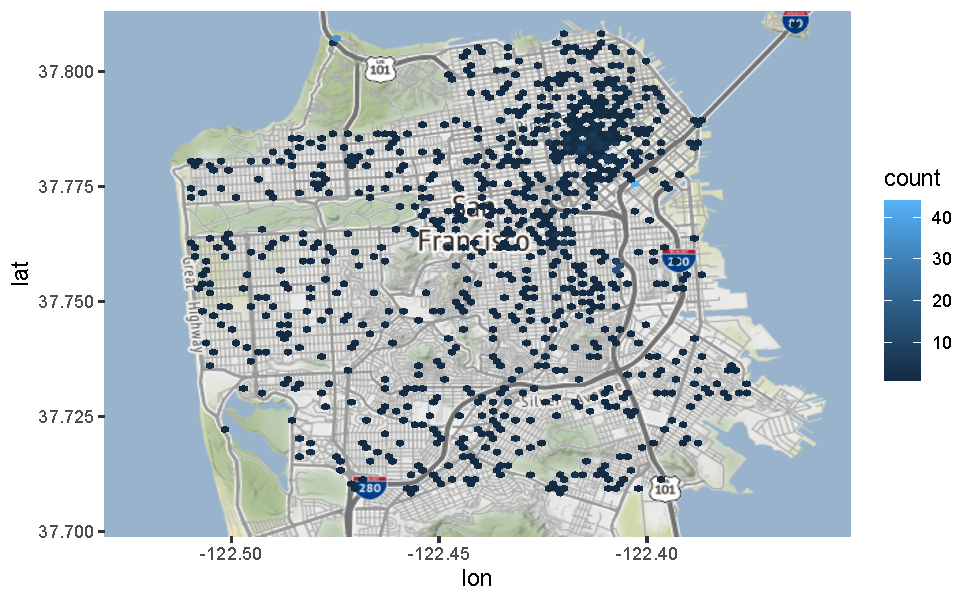
\includegraphics[width=0.9\linewidth]{crimebythenumbers_files/figure-latex/unnamed-chunk-14-1} \end{center}

Running the above code returns a blank graph since we haven't told \texttt{ggplot()} what type of graph we want yet. Below are a few different types of ways to display a single numeric variable. They're essentially all variations of each other and show the data at different levels of precision. It's hard to say which is best - you'll need to use your best judgment and consider your audience.

\hypertarget{histogram}{%
\subsection{Histogram}\label{histogram}}

The histogram is a very common type of graph for a single numeric variable. Histograms group a numeric variable into categories and then plot then, with the heights of each bar indicating how common the group is. We can make a histogram by adding \texttt{geom\_histogram()} to the \texttt{ggplot()}.

\begin{Shaded}
\begin{Highlighting}[]
\FunctionTok{ggplot}\NormalTok{(shootings, }\FunctionTok{aes}\NormalTok{(}\AttributeTok{x =}\NormalTok{ age)) }\SpecialCharTok{+} 
  \FunctionTok{geom\_histogram}\NormalTok{()}
\CommentTok{\#\textgreater{} \textasciigrave{}stat\_bin()\textasciigrave{} using \textasciigrave{}bins = 30\textasciigrave{}. Pick better value}
\CommentTok{\#\textgreater{} with \textasciigrave{}binwidth\textasciigrave{}.}
\CommentTok{\#\textgreater{} Warning: Removed 280 rows containing non{-}finite values}
\CommentTok{\#\textgreater{} (stat\_bin).}
\end{Highlighting}
\end{Shaded}

\begin{center}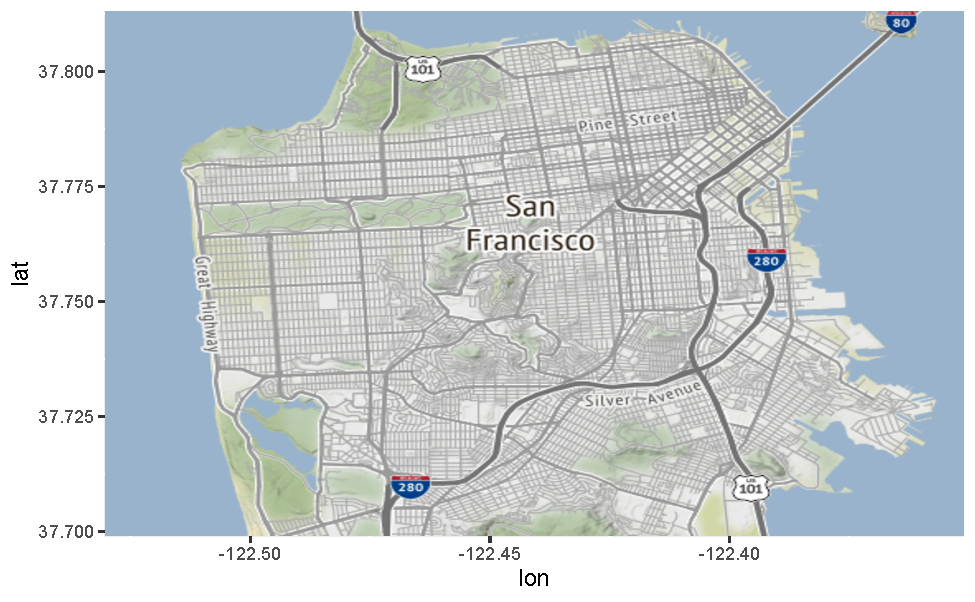
\includegraphics[width=0.9\linewidth]{crimebythenumbers_files/figure-latex/unnamed-chunk-15-1} \end{center}

The x-axis is ages with each bar being a group of certain ages, and the y-axis is how many people are in each group. The grouping is done automatically and we can alter it by changing the \texttt{bin} parameter in \texttt{geom\_histogram()}. By default this parameter is set to 30 but we can make each group smaller (have fewer ages per group) by \textbf{increasing} it from 30 or make each group larger by \textbf{decreasing} it.

\begin{Shaded}
\begin{Highlighting}[]
\FunctionTok{ggplot}\NormalTok{(shootings, }\FunctionTok{aes}\NormalTok{(}\AttributeTok{x =}\NormalTok{ age)) }\SpecialCharTok{+} 
  \FunctionTok{geom\_histogram}\NormalTok{(}\AttributeTok{bins =} \DecValTok{15}\NormalTok{)}
\CommentTok{\#\textgreater{} Warning: Removed 280 rows containing non{-}finite values}
\CommentTok{\#\textgreater{} (stat\_bin).}
\end{Highlighting}
\end{Shaded}

\begin{center}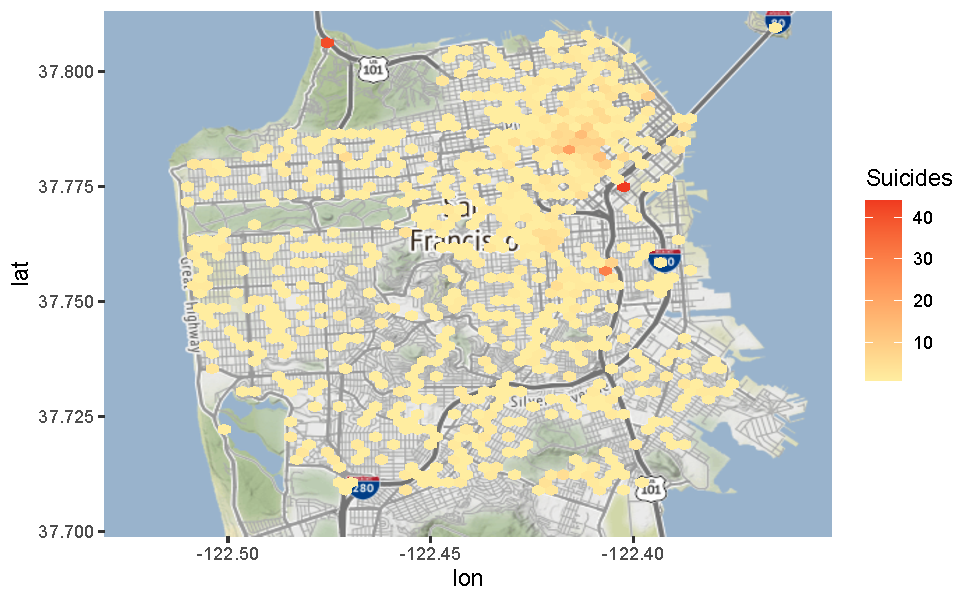
\includegraphics[width=0.9\linewidth]{crimebythenumbers_files/figure-latex/unnamed-chunk-16-1} \end{center}

\begin{Shaded}
\begin{Highlighting}[]
\FunctionTok{ggplot}\NormalTok{(shootings, }\FunctionTok{aes}\NormalTok{(}\AttributeTok{x =}\NormalTok{ age)) }\SpecialCharTok{+} 
  \FunctionTok{geom\_histogram}\NormalTok{(}\AttributeTok{bins =} \DecValTok{45}\NormalTok{)}
\CommentTok{\#\textgreater{} Warning: Removed 280 rows containing non{-}finite values}
\CommentTok{\#\textgreater{} (stat\_bin).}
\end{Highlighting}
\end{Shaded}

\begin{center}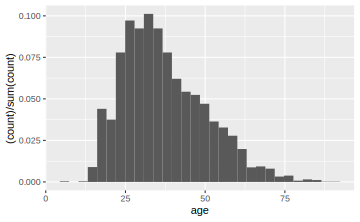
\includegraphics[width=0.9\linewidth]{crimebythenumbers_files/figure-latex/unnamed-chunk-17-1} \end{center}

Note that while the overall trend (of most deaths being around age 25) doesn't change when we alter \texttt{bin}, the data gets more or less precise. Having fewer bins means fewer, but larger, bars which can obscure trends that more, smaller, bars would show. But having too many bars may make you focus on minor variations that could occur randomly and take away attention from the overall trend. I prefer to err on the side of more precise graphs (more, smaller bars) but be careful over-interpreting data from small groups.

These graphs show the y-axis as the number of people in each bar. If we want to show percent instead, we can add in a parameter for \texttt{y} in the \texttt{aes()} of the \texttt{geom\_histogram()}. We add in \texttt{y\ =\ (..count..)/sum(..count..))} which automatically converts the counts to percentages. The ``(..count..)/sum(..count..))'' stuff is just taking each group and dividing it from the sum of all groups. You could, of course, do this yourself before making the graph, but it's an easy helper. If you do this, make sure to relabel the y-axis so you don't accidentally call the percent a count!

\begin{Shaded}
\begin{Highlighting}[]
\FunctionTok{ggplot}\NormalTok{(shootings, }\FunctionTok{aes}\NormalTok{(}\AttributeTok{x =}\NormalTok{ age)) }\SpecialCharTok{+} 
  \FunctionTok{geom\_histogram}\NormalTok{(}\FunctionTok{aes}\NormalTok{(}\AttributeTok{y =}\NormalTok{ (..count..)}\SpecialCharTok{/}\FunctionTok{sum}\NormalTok{(..count..)))}
\CommentTok{\#\textgreater{} \textasciigrave{}stat\_bin()\textasciigrave{} using \textasciigrave{}bins = 30\textasciigrave{}. Pick better value}
\CommentTok{\#\textgreater{} with \textasciigrave{}binwidth\textasciigrave{}.}
\CommentTok{\#\textgreater{} Warning: Removed 280 rows containing non{-}finite values}
\CommentTok{\#\textgreater{} (stat\_bin).}
\end{Highlighting}
\end{Shaded}

\begin{center}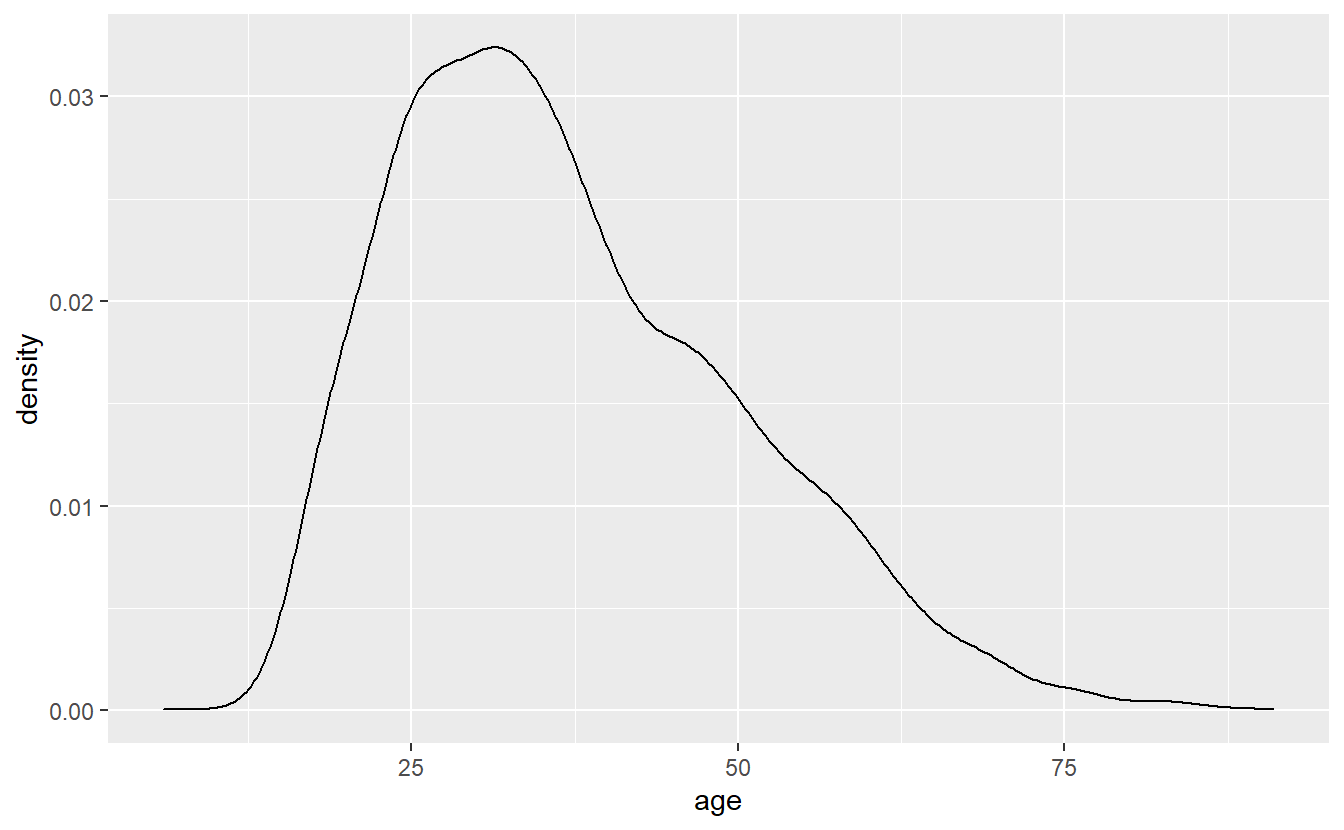
\includegraphics[width=0.9\linewidth]{crimebythenumbers_files/figure-latex/unnamed-chunk-18-1} \end{center}

\hypertarget{density-plot}{%
\subsection{Density plot}\label{density-plot}}

Density plots are essentially smoothed versions of histograms. They're especially useful for numeric variables which are not integers (integers are whole numbers). They're also useful when you want to be more precise than a histogram as they are - to simplify - histograms where each bar is very narrow. Note that the y-axis of a density plot is automatically labeled ``density'' and has very small numbers. Interpreting the y-axis is fairly hard to explain to someone not familiar with statistics so I'd caution against using this graph unless your audience is already familiar with it. To interpret these kinds of graphs, I recommend looking for trends rather than trying to identify specific points. For example, in the below graph we can see that shootings rise rapidly starting around age 10, peak at around age 30 (if we were presenting this graph to other people we'd probably want more ages shown on the x-axis), and then steadily decline until about age 80 where it's nearly flat.

\begin{Shaded}
\begin{Highlighting}[]
\FunctionTok{ggplot}\NormalTok{(shootings, }\FunctionTok{aes}\NormalTok{(}\AttributeTok{x =}\NormalTok{ age)) }\SpecialCharTok{+} 
  \FunctionTok{geom\_density}\NormalTok{()}
\CommentTok{\#\textgreater{} Warning: Removed 280 rows containing non{-}finite values}
\CommentTok{\#\textgreater{} (stat\_density).}
\end{Highlighting}
\end{Shaded}

\begin{center}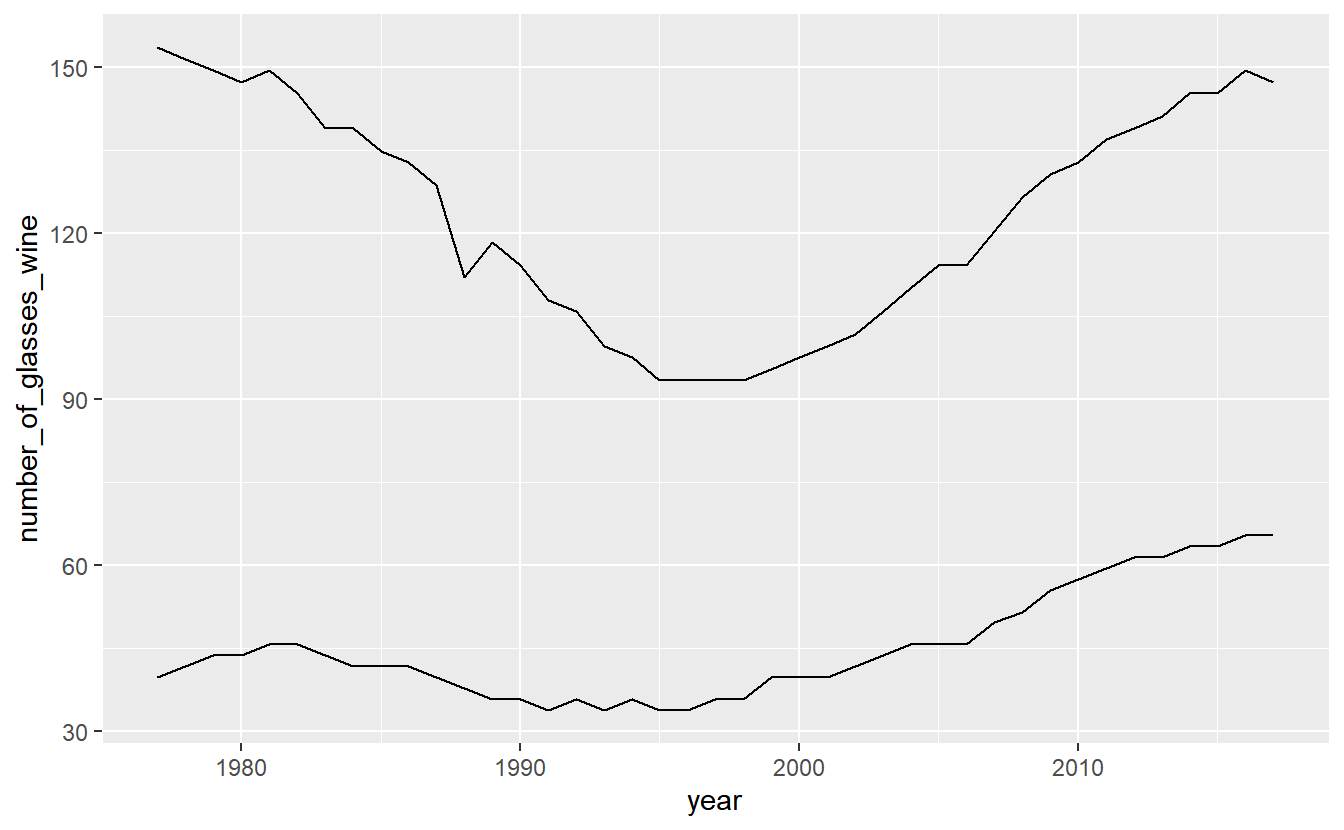
\includegraphics[width=0.9\linewidth]{crimebythenumbers_files/figure-latex/unnamed-chunk-19-1} \end{center}

\hypertarget{count-graph}{%
\subsection{Count Graph}\label{count-graph}}

A count graph is essentially a histogram with a bar for every value in the numeric variable - like a less-smooth density plot. Note that this won't work well if you have too many unique values so I'd strongly recommend rounding the data to the nearest whole number first. Our age variable is already rounded so we don't need to do that. To make a count graph, we add \texttt{stat\_count()} to the \texttt{ggplot()}.

\begin{Shaded}
\begin{Highlighting}[]
\FunctionTok{ggplot}\NormalTok{(shootings, }\FunctionTok{aes}\NormalTok{(}\AttributeTok{x =}\NormalTok{ age)) }\SpecialCharTok{+} 
  \FunctionTok{stat\_count}\NormalTok{()}
\CommentTok{\#\textgreater{} Warning: Removed 280 rows containing non{-}finite values}
\CommentTok{\#\textgreater{} (stat\_count).}
\end{Highlighting}
\end{Shaded}

\begin{center}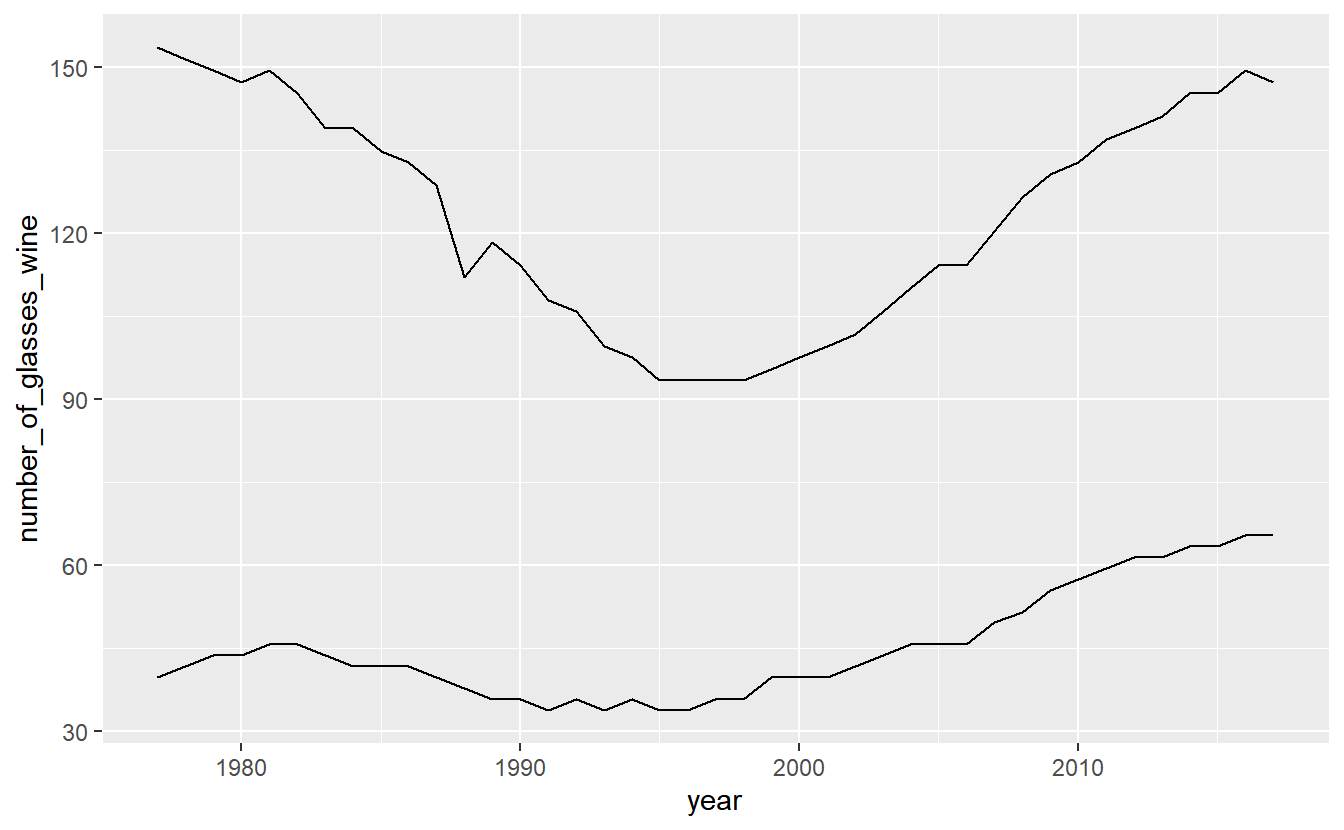
\includegraphics[width=0.9\linewidth]{crimebythenumbers_files/figure-latex/unnamed-chunk-20-1} \end{center}

Now we have a single bar for every age in the data. Like the histogram, the y-axis shows the number of people that are that age. And like the histogram, we can change this from number of people to percent of people using the exact same code.

\begin{Shaded}
\begin{Highlighting}[]
\FunctionTok{ggplot}\NormalTok{(shootings, }\FunctionTok{aes}\NormalTok{(}\AttributeTok{x =}\NormalTok{ age)) }\SpecialCharTok{+} 
  \FunctionTok{stat\_count}\NormalTok{(}\FunctionTok{aes}\NormalTok{(}\AttributeTok{y =}\NormalTok{ (..count..)}\SpecialCharTok{/}\FunctionTok{sum}\NormalTok{(..count..)))}
\CommentTok{\#\textgreater{} Warning: Removed 280 rows containing non{-}finite values}
\CommentTok{\#\textgreater{} (stat\_count).}
\end{Highlighting}
\end{Shaded}

\begin{center}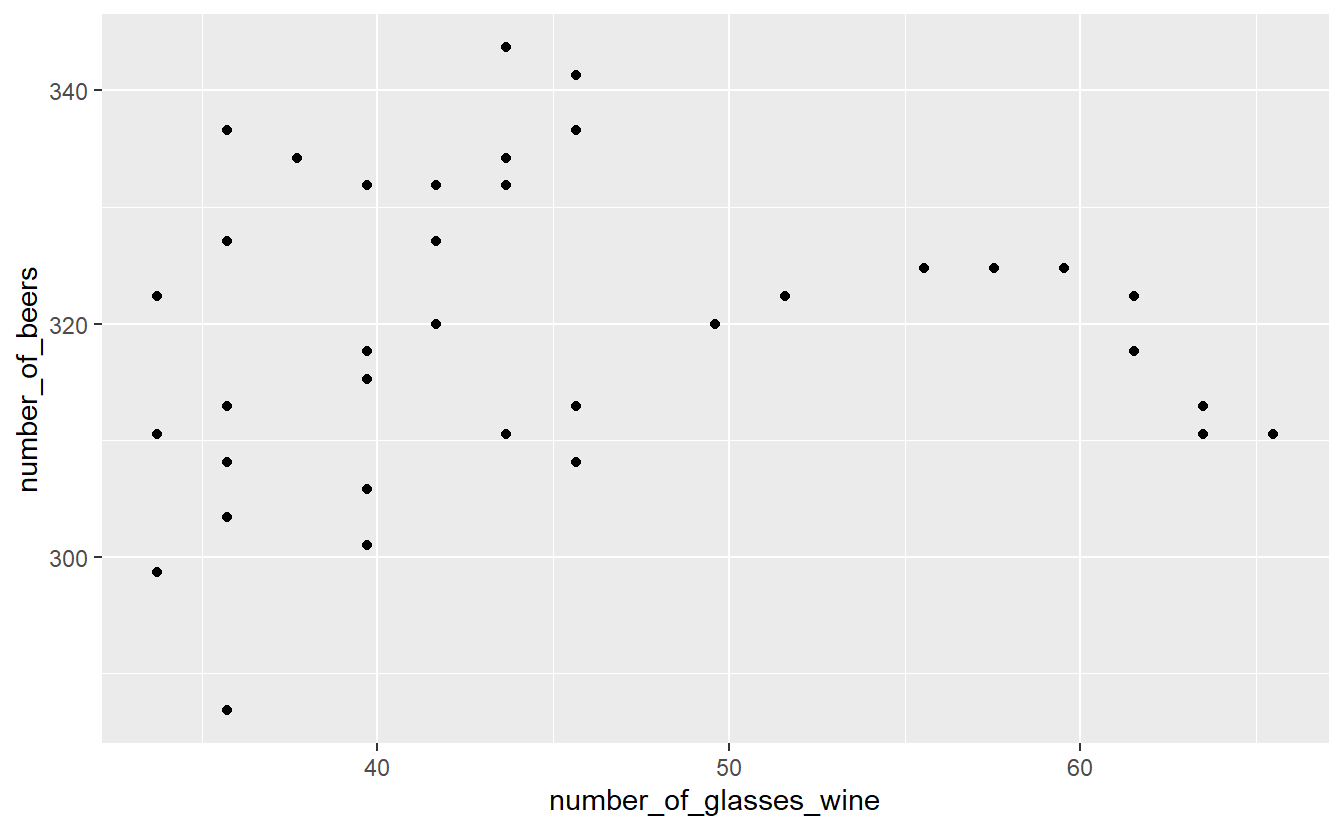
\includegraphics[width=0.9\linewidth]{crimebythenumbers_files/figure-latex/unnamed-chunk-21-1} \end{center}

\hypertarget{graphing-a-categorical-variable}{%
\subsection{Graphing a Categorical Variable}\label{graphing-a-categorical-variable}}

\hypertarget{bar-graph}{%
\section{Bar graph}\label{bar-graph}}

To make this barplot we'll set the x-axis variable to our ``race'' column and add \texttt{geom\_bar()} to the end.

\begin{Shaded}
\begin{Highlighting}[]
\FunctionTok{ggplot}\NormalTok{(shootings, }\FunctionTok{aes}\NormalTok{(}\AttributeTok{x =}\NormalTok{ race)) }\SpecialCharTok{+} 
  \FunctionTok{geom\_bar}\NormalTok{()}
\end{Highlighting}
\end{Shaded}

\begin{center}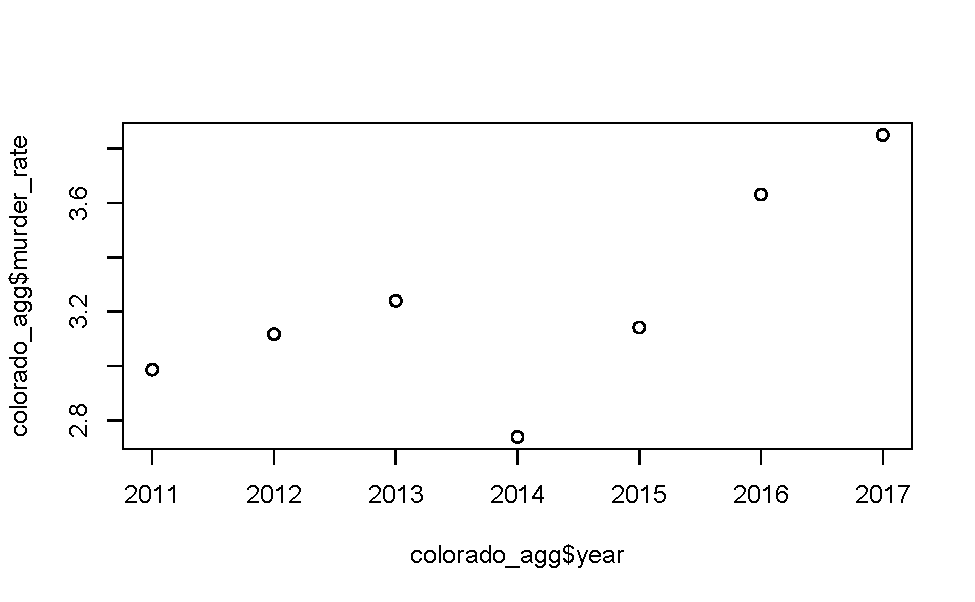
\includegraphics[width=0.9\linewidth]{crimebythenumbers_files/figure-latex/unnamed-chunk-22-1} \end{center}

This gives us a barplot in alphabetical order. In most cases we want the data sorted by frequency, so we can easily see what value is the most common, second most common, etc. There are a few ways to do this but we'll do this by turning the ``race'' variable into a factor and ordering it by frequency. We can do that using the \texttt{factor()} function. The first input will be the ``race'' variable and then we will need to set the \texttt{levels} parameter to a vector of values sorted by frequency. An easy way to know how often values are in a column is to use the \texttt{table()} function on that column, such as below.

\begin{Shaded}
\begin{Highlighting}[]
\FunctionTok{table}\NormalTok{(shootings}\SpecialCharTok{$}\NormalTok{race)}
\CommentTok{\#\textgreater{} }
\CommentTok{\#\textgreater{}    A    B    H    N    O    W }
\CommentTok{\#\textgreater{}  104 1499 1052   87   47 2885}
\end{Highlighting}
\end{Shaded}

It's still alphabetical so let's wrap that in a \texttt{sort()} function.

\begin{Shaded}
\begin{Highlighting}[]
\FunctionTok{sort}\NormalTok{(}\FunctionTok{table}\NormalTok{(shootings}\SpecialCharTok{$}\NormalTok{race))}
\CommentTok{\#\textgreater{} }
\CommentTok{\#\textgreater{}    O    N    A    H    B    W }
\CommentTok{\#\textgreater{}   47   87  104 1052 1499 2885}
\end{Highlighting}
\end{Shaded}

It's sorted from smallest to largest. We usually want to graph from largest to smallest so let's set the parameter \texttt{decreasing} in \texttt{sort()} to TRUE.

\begin{Shaded}
\begin{Highlighting}[]
\FunctionTok{sort}\NormalTok{(}\FunctionTok{table}\NormalTok{(shootings}\SpecialCharTok{$}\NormalTok{race), }\AttributeTok{decreasing =} \ConstantTok{TRUE}\NormalTok{)}
\CommentTok{\#\textgreater{} }
\CommentTok{\#\textgreater{}    W    B    H    A    N    O }
\CommentTok{\#\textgreater{} 2885 1499 1052  104   87   47}
\end{Highlighting}
\end{Shaded}

Now, we only need the names of each value, not how often they occur. So we can against wrap this whole thing in \texttt{names()} to get just the names.

\begin{Shaded}
\begin{Highlighting}[]
\FunctionTok{names}\NormalTok{(}\FunctionTok{sort}\NormalTok{(}\FunctionTok{table}\NormalTok{(shootings}\SpecialCharTok{$}\NormalTok{race), }\AttributeTok{decreasing =} \ConstantTok{TRUE}\NormalTok{))}
\CommentTok{\#\textgreater{} [1] "W" "B" "H" "A" "N" "O"}
\end{Highlighting}
\end{Shaded}

If we tie it all together, we can make the ``race'' column into a factor variable.

\begin{Shaded}
\begin{Highlighting}[]
\NormalTok{shootings}\SpecialCharTok{$}\NormalTok{race }\OtherTok{\textless{}{-}} \FunctionTok{factor}\NormalTok{(shootings}\SpecialCharTok{$}\NormalTok{race,}
                         \AttributeTok{levels =} \FunctionTok{names}\NormalTok{(}\FunctionTok{sort}\NormalTok{(}\FunctionTok{table}\NormalTok{(shootings}\SpecialCharTok{$}\NormalTok{race), }\AttributeTok{decreasing =} \ConstantTok{TRUE}\NormalTok{)))}
\end{Highlighting}
\end{Shaded}

Now let's try that barplot again.

\begin{Shaded}
\begin{Highlighting}[]
\FunctionTok{ggplot}\NormalTok{(shootings, }\FunctionTok{aes}\NormalTok{(}\AttributeTok{x =}\NormalTok{ race)) }\SpecialCharTok{+} 
  \FunctionTok{geom\_bar}\NormalTok{() }
\end{Highlighting}
\end{Shaded}

\begin{center}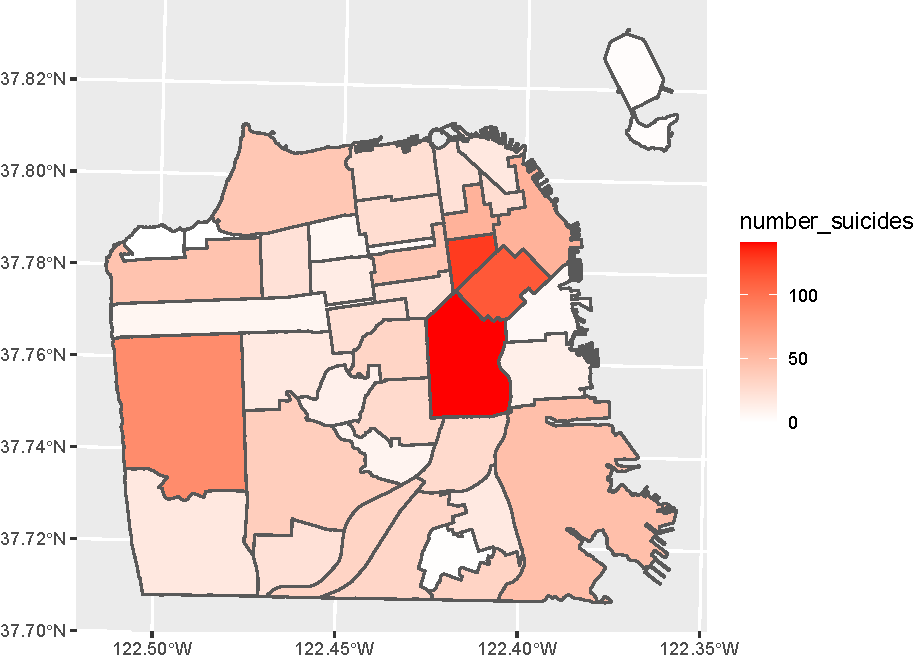
\includegraphics[width=0.9\linewidth]{crimebythenumbers_files/figure-latex/unnamed-chunk-28-1} \end{center}

It works! Note that all the values that are missing in our data are still reported in the barplot under a column called ``NA''. This is not sorted properly since there are more NA values than three of the other values but is still at the far right of the graph. We can change this if we want to make all the NA values an actual character type and call it something like ``Unknown''. But this way it does draw attention to how many values are missing from this column. Like most things in graphing, this is a personal choice as to what to do.

For bar graphs it is often useful to flip the graph so each value is a row in the graph rather than a column. This also makes it much easier to read the value name. If the value names are long, it'll shrink the graph to accommodate the name. This is usually a sign that you should try to shorten the name to avoid reducing the size of the graph.

\begin{Shaded}
\begin{Highlighting}[]
\FunctionTok{ggplot}\NormalTok{(shootings, }\FunctionTok{aes}\NormalTok{(}\AttributeTok{x =}\NormalTok{ race)) }\SpecialCharTok{+} 
  \FunctionTok{geom\_bar}\NormalTok{() }\SpecialCharTok{+}
  \FunctionTok{coord\_flip}\NormalTok{() }
\end{Highlighting}
\end{Shaded}

\begin{center}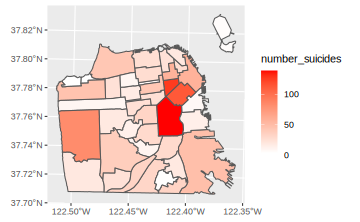
\includegraphics[width=0.9\linewidth]{crimebythenumbers_files/figure-latex/unnamed-chunk-29-1} \end{center}

Since it's flipped, now it's sorted from smallest to largest. So we'll need to change the \texttt{factor()} code to fix that.

\begin{Shaded}
\begin{Highlighting}[]
\NormalTok{shootings}\SpecialCharTok{$}\NormalTok{race }\OtherTok{\textless{}{-}} \FunctionTok{factor}\NormalTok{(shootings}\SpecialCharTok{$}\NormalTok{race,}
                         \AttributeTok{levels =} \FunctionTok{names}\NormalTok{(}\FunctionTok{sort}\NormalTok{(}\FunctionTok{table}\NormalTok{(shootings}\SpecialCharTok{$}\NormalTok{race), }\AttributeTok{decreasing =} \ConstantTok{FALSE}\NormalTok{)))}
\FunctionTok{ggplot}\NormalTok{(shootings, }\FunctionTok{aes}\NormalTok{(}\AttributeTok{x =}\NormalTok{ race)) }\SpecialCharTok{+} 
  \FunctionTok{geom\_bar}\NormalTok{() }\SpecialCharTok{+}
  \FunctionTok{coord\_flip}\NormalTok{() }
\end{Highlighting}
\end{Shaded}

\begin{center}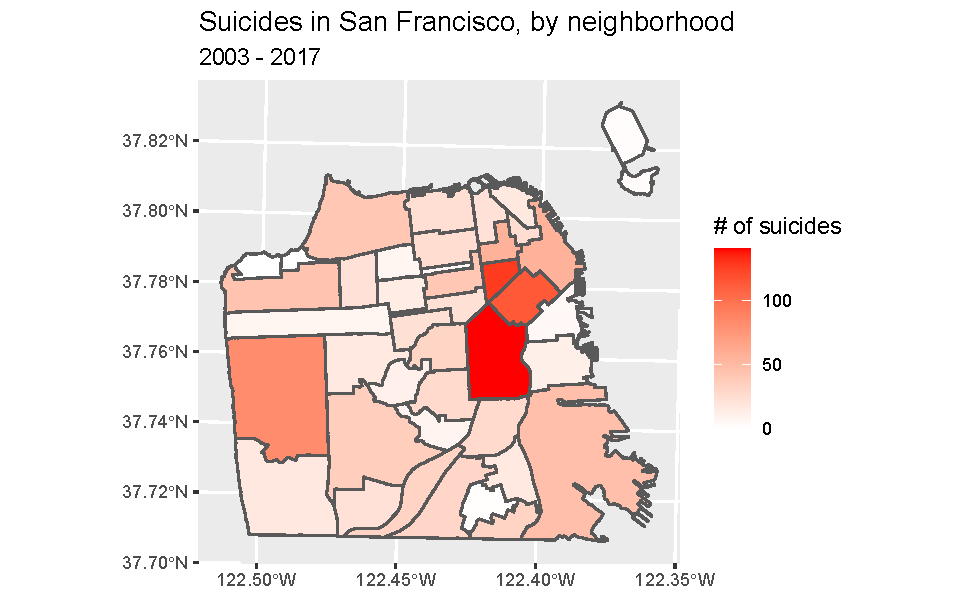
\includegraphics[width=0.9\linewidth]{crimebythenumbers_files/figure-latex/unnamed-chunk-30-1} \end{center}

The NA value is now at the top, which looks fairly bad. Let's change all NA values to the string ``Unknown''. And while we're at it, let's change all the abbreviated race values to actual names. We can get all the NA values by using \texttt{is.na(shootings\$race)} and using a conditional statement to get all rows that meet that condition, then assign them the value ``Unknown''. Instead of trying to subset a factor variable to change the values, we should convert it back to a character type first using \texttt{as.character()}, and then convert it to a factor again once we're done.

\begin{Shaded}
\begin{Highlighting}[]
\NormalTok{shootings}\SpecialCharTok{$}\NormalTok{race }\OtherTok{\textless{}{-}} \FunctionTok{as.character}\NormalTok{(shootings}\SpecialCharTok{$}\NormalTok{race)}
\NormalTok{shootings}\SpecialCharTok{$}\NormalTok{race[}\FunctionTok{is.na}\NormalTok{(shootings}\SpecialCharTok{$}\NormalTok{race)] }\OtherTok{\textless{}{-}} \StringTok{"Unknown"}
\end{Highlighting}
\end{Shaded}

Now we can use conditional statements to change all the race letters to names. It's not clear what race ``O'' and ``N'' are so I checked the \href{https://github.com/washingtonpost/data-police-shootings}{Washington Post's GitHub page} which explains. Instead of \texttt{is.na()} we'll use \texttt{shootings\$race\ ==\ ""} where we put the letter inside of the quotes.

\begin{Shaded}
\begin{Highlighting}[]
\NormalTok{shootings}\SpecialCharTok{$}\NormalTok{race[shootings}\SpecialCharTok{$}\NormalTok{race }\SpecialCharTok{==} \StringTok{"O"}\NormalTok{] }\OtherTok{\textless{}{-}} \StringTok{"Other"}
\NormalTok{shootings}\SpecialCharTok{$}\NormalTok{race[shootings}\SpecialCharTok{$}\NormalTok{race }\SpecialCharTok{==} \StringTok{"N"}\NormalTok{] }\OtherTok{\textless{}{-}} \StringTok{"Native American"}
\NormalTok{shootings}\SpecialCharTok{$}\NormalTok{race[shootings}\SpecialCharTok{$}\NormalTok{race }\SpecialCharTok{==} \StringTok{"A"}\NormalTok{] }\OtherTok{\textless{}{-}} \StringTok{"Asian"}
\NormalTok{shootings}\SpecialCharTok{$}\NormalTok{race[shootings}\SpecialCharTok{$}\NormalTok{race }\SpecialCharTok{==} \StringTok{"H"}\NormalTok{] }\OtherTok{\textless{}{-}} \StringTok{"Hispanic"}
\NormalTok{shootings}\SpecialCharTok{$}\NormalTok{race[shootings}\SpecialCharTok{$}\NormalTok{race }\SpecialCharTok{==} \StringTok{"B"}\NormalTok{] }\OtherTok{\textless{}{-}} \StringTok{"Black"}
\NormalTok{shootings}\SpecialCharTok{$}\NormalTok{race[shootings}\SpecialCharTok{$}\NormalTok{race }\SpecialCharTok{==} \StringTok{"W"}\NormalTok{] }\OtherTok{\textless{}{-}} \StringTok{"White"}
\end{Highlighting}
\end{Shaded}

Now let's see how our graph looks. We'll need to rerun the \texttt{factor()} code since now all of the values are changed.

\begin{Shaded}
\begin{Highlighting}[]
\NormalTok{shootings}\SpecialCharTok{$}\NormalTok{race }\OtherTok{\textless{}{-}} \FunctionTok{factor}\NormalTok{(shootings}\SpecialCharTok{$}\NormalTok{race,}
                         \AttributeTok{levels =} \FunctionTok{names}\NormalTok{(}\FunctionTok{sort}\NormalTok{(}\FunctionTok{table}\NormalTok{(shootings}\SpecialCharTok{$}\NormalTok{race), }\AttributeTok{decreasing =} \ConstantTok{FALSE}\NormalTok{)))}
\FunctionTok{ggplot}\NormalTok{(shootings, }\FunctionTok{aes}\NormalTok{(}\AttributeTok{x =}\NormalTok{ race)) }\SpecialCharTok{+} 
  \FunctionTok{geom\_bar}\NormalTok{() }\SpecialCharTok{+}
  \FunctionTok{coord\_flip}\NormalTok{() }
\end{Highlighting}
\end{Shaded}

\begin{center}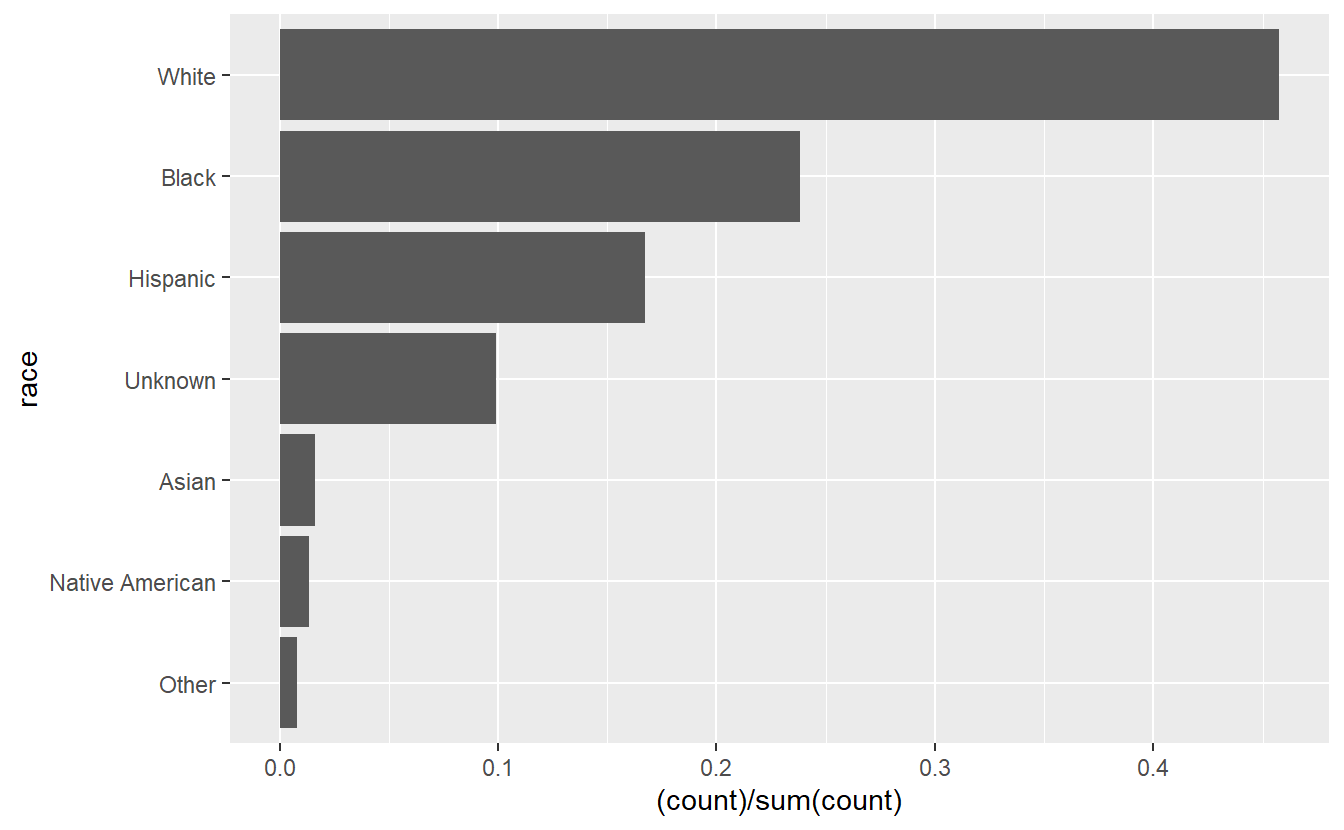
\includegraphics[width=0.9\linewidth]{crimebythenumbers_files/figure-latex/unnamed-chunk-33-1} \end{center}

As earlier, we can show percentage instead of count by adding \texttt{y\ =\ (..count..)/sum(..count..)} to the \texttt{aes()} in \texttt{geom\_bar()}.

\begin{Shaded}
\begin{Highlighting}[]
\FunctionTok{ggplot}\NormalTok{(shootings, }\FunctionTok{aes}\NormalTok{(}\AttributeTok{x =}\NormalTok{ race)) }\SpecialCharTok{+} 
  \FunctionTok{geom\_bar}\NormalTok{(}\FunctionTok{aes}\NormalTok{(}\AttributeTok{y =}\NormalTok{ (..count..)}\SpecialCharTok{/}\FunctionTok{sum}\NormalTok{(..count..))) }\SpecialCharTok{+}
  \FunctionTok{coord\_flip}\NormalTok{() }
\end{Highlighting}
\end{Shaded}

\begin{center}\includegraphics[width=0.9\linewidth]{crimebythenumbers_files/figure-latex/unnamed-chunk-34-1} \end{center}

\hypertarget{graphing-data-over-time}{%
\section{Graphing Data Over Time}\label{graphing-data-over-time}}

We went over time-series graphs in Chapter \ref{graphing-intro} but it's such an important topic we'll cover it again. A lot of criminology research is seeing if a policy had an effect, which means we generally want to compare an outcome over time (and compare the treated group to a similar untreated group). To graph that we look at an outcome, in this case numbers of killings, over time. In our case we aren't evaluating any policy, just seeing if the number of police killings change over time.

We'll need to make a variable to indicate that the row is for one shooting. We can call this ``dummy'' and assign it a value of 1. Then we can make the \texttt{ggplot()} and set this ``dummy'' column to the y-axis value and set our date variable ``date'' to the x-axis (the time variable is \textbf{always} on the x-axis). Then we'll set the type of plot to \texttt{geom\_line()} so we have a line graph showing killings over time.

\begin{Shaded}
\begin{Highlighting}[]
\NormalTok{shootings}\SpecialCharTok{$}\NormalTok{dummy }\OtherTok{\textless{}{-}} \DecValTok{1}
\FunctionTok{ggplot}\NormalTok{(shootings, }\FunctionTok{aes}\NormalTok{(}\AttributeTok{x =}\NormalTok{ date, }\AttributeTok{y =}\NormalTok{ dummy)) }\SpecialCharTok{+}
  \FunctionTok{geom\_line}\NormalTok{()}
\end{Highlighting}
\end{Shaded}

\begin{center}\includegraphics[width=0.9\linewidth]{crimebythenumbers_files/figure-latex/unnamed-chunk-35-1} \end{center}

This graph is clearly wrong. Why? Well, our y-axis variable is always 1 so there's no variation to plot. Every single value, even if there are more than one shooting per day, is on the 1 line on the y-axis. And the fact that we have multiple killings per day is an issue because we only want a single line in our graph. We'll need to aggregate our data to some time period (e.g.~day, month, year) so that we have one row per time-period and know how many people were killed in that period. We'll start with yearly data and then move to monthly data. Since we're going to be dealing with dates, lets load the \texttt{lubridate()} package that is well-suited for this task.

\begin{Shaded}
\begin{Highlighting}[]
\FunctionTok{library}\NormalTok{(lubridate)}
\CommentTok{\#\textgreater{} }
\CommentTok{\#\textgreater{} Attaching package: \textquotesingle{}lubridate\textquotesingle{}}
\CommentTok{\#\textgreater{} The following objects are masked from \textquotesingle{}package:base\textquotesingle{}:}
\CommentTok{\#\textgreater{} }
\CommentTok{\#\textgreater{}     date, intersect, setdiff, union}
\end{Highlighting}
\end{Shaded}

We'll use two functions to create variables that tell us the month and the year of each date in our data. We'll use these new variables to aggregate our data to that time unit. First, the \texttt{floor\_date()} function is a very useful tool that essentially rounds a date. Here we have the exact date the killing happened on, and we want to determine what month that date is from. So we'll use the parameter \texttt{unit} in \texttt{floor\_date()} and tell the function we want to know the ``month'' (for a full set of options please see the documentation for \texttt{floor\_date()} by entering \texttt{?floor\_date} in the console). So we can do \texttt{floor\_date(shootings\$date,\ unit\ =\ "month")} to get the month - specifically, it returns the date that is the first of the month for that month - the killing happened on. Even simpler, to get the year, we simple use \texttt{year()} and put our ``date'' variable in the parentheses. We'll call the new variables ``month\_year'' and ``year'', respectively.

\begin{Shaded}
\begin{Highlighting}[]
\NormalTok{shootings}\SpecialCharTok{$}\NormalTok{month\_year }\OtherTok{\textless{}{-}} \FunctionTok{floor\_date}\NormalTok{(shootings}\SpecialCharTok{$}\NormalTok{date, }\AttributeTok{unit =} \StringTok{"month"}\NormalTok{)}
\NormalTok{shootings}\SpecialCharTok{$}\NormalTok{year }\OtherTok{\textless{}{-}} \FunctionTok{year}\NormalTok{(shootings}\SpecialCharTok{$}\NormalTok{date)}

\FunctionTok{head}\NormalTok{(shootings}\SpecialCharTok{$}\NormalTok{month\_year)}
\CommentTok{\#\textgreater{} [1] "2015{-}01{-}01" "2015{-}01{-}01" "2015{-}01{-}01" "2015{-}01{-}01"}
\CommentTok{\#\textgreater{} [5] "2015{-}01{-}01" "2015{-}01{-}01"}
\FunctionTok{head}\NormalTok{(shootings}\SpecialCharTok{$}\NormalTok{year)}
\CommentTok{\#\textgreater{} [1] 2015 2015 2015 2015 2015 2015}
\end{Highlighting}
\end{Shaded}

Since the data is already sorted by date, all the values printed from \texttt{head()} are the same. But you can look at the data using \texttt{View()} to confirm that the code worked properly.

We can now aggregate the data by the ``month\_year'' variable and save the result into a new dataset we'll call \emph{monthly\_shootings}. For a refresher on aggregating, please see Section \ref{aggregate}

\begin{Shaded}
\begin{Highlighting}[]
\NormalTok{monthly\_shootings }\OtherTok{\textless{}{-}} \FunctionTok{aggregate}\NormalTok{(dummy }\SpecialCharTok{\textasciitilde{}}\NormalTok{ month\_year, }\AttributeTok{data =}\NormalTok{ shootings, }\AttributeTok{FUN =}\NormalTok{ sum)}
\FunctionTok{head}\NormalTok{(monthly\_shootings)}
\CommentTok{\#\textgreater{}   month\_year dummy}
\CommentTok{\#\textgreater{} 1 2015{-}01{-}01    76}
\CommentTok{\#\textgreater{} 2 2015{-}02{-}01    77}
\CommentTok{\#\textgreater{} 3 2015{-}03{-}01    92}
\CommentTok{\#\textgreater{} 4 2015{-}04{-}01    84}
\CommentTok{\#\textgreater{} 5 2015{-}05{-}01    71}
\CommentTok{\#\textgreater{} 6 2015{-}06{-}01    65}
\end{Highlighting}
\end{Shaded}

Since we now have a variable that shows for each month the number of people killed, we can graph this new dataset. We'll use the same process as earlier but our dataset is now \texttt{monthly\_shootings} instead of \texttt{shootings} and the x-axis variable is ``month\_year'' instead of ``date''.

\begin{Shaded}
\begin{Highlighting}[]
\FunctionTok{ggplot}\NormalTok{(monthly\_shootings, }\FunctionTok{aes}\NormalTok{(}\AttributeTok{x =}\NormalTok{ month\_year, }\AttributeTok{y =}\NormalTok{ dummy)) }\SpecialCharTok{+}
  \FunctionTok{geom\_line}\NormalTok{()}
\end{Highlighting}
\end{Shaded}

\begin{center}\includegraphics[width=0.9\linewidth]{crimebythenumbers_files/figure-latex/unnamed-chunk-39-1} \end{center}

The process is the same for yearly data.

\begin{Shaded}
\begin{Highlighting}[]
\NormalTok{yearly\_shootings }\OtherTok{\textless{}{-}} \FunctionTok{aggregate}\NormalTok{(dummy }\SpecialCharTok{\textasciitilde{}}\NormalTok{ year, }\AttributeTok{data =}\NormalTok{ shootings, }\AttributeTok{FUN =}\NormalTok{ sum)}
\FunctionTok{ggplot}\NormalTok{(yearly\_shootings, }\FunctionTok{aes}\NormalTok{(}\AttributeTok{x =}\NormalTok{ year, }\AttributeTok{y =}\NormalTok{ dummy)) }\SpecialCharTok{+}
  \FunctionTok{geom\_line}\NormalTok{()}
\end{Highlighting}
\end{Shaded}

\begin{center}\includegraphics[width=0.9\linewidth]{crimebythenumbers_files/figure-latex/unnamed-chunk-40-1} \end{center}

Note the steep drop-off at the end of each graph. Is that due to fewer shooting occurring more recently? No, it's simply an artifact of the graph comparing whole months (years) to parts of a month (year) since we haven't finished this month (year) yet (and the data has a small lag in reporting).

\hypertarget{pretty-graphs}{%
\section{Pretty Graphs}\label{pretty-graphs}}

What's next for these graphs? You'll likely want to add labels for the axes and the title. We went over how to do this in Section \ref{time-series-plots} so please refer to that for more info. Also, check out \texttt{ggplot2}'s \href{https://ggplot2.tidyverse.org/reference/index.html\#section-scales}{website} to see more on this very versatile package. As I've said all chapter, a lot of this is going to be personal taste so please spend some time exploring the package and changing the appearance of the graph to learn what looks right to you.

\hypertarget{themes}{%
\subsection{Themes}\label{themes}}

In addition to making changes to the graph's appearance yourself, you can use a theme that someone else made. A theme is just a collection of changes to the graph's appearance that someone put in a function for others to use. Each theme is different and is fairly opinionated, so you should only use one that you think looks best for your graph. To use a theme, simply add the theme (exactly as spelled on the site) to your ggplot using the + as normal (and make sure to include the () since each theme is actually a function. \texttt{ggplot2} comes with a series of themes that you can look at \href{https://ggplot2.tidyverse.org/reference/ggtheme.html}{here}. Here, we'll be looking at themes from the \texttt{ggthemes} package which is a great source of different themes to modify the appearance of your graph. Check out this \href{https://yutannihilation.github.io/allYourFigureAreBelongToUs/ggthemes/}{website} to see a depiction of all of the possible themes. If you don't have the \texttt{ggthemes} package installed, do so using `install.packages(``ggthemes'').

Let's do a few examples using the graph made above. First, we'll need to load the \texttt{ggthemes} library.

\begin{Shaded}
\begin{Highlighting}[]
\FunctionTok{library}\NormalTok{(ggthemes)}
\FunctionTok{ggplot}\NormalTok{(yearly\_shootings, }\FunctionTok{aes}\NormalTok{(}\AttributeTok{x =}\NormalTok{ year, }\AttributeTok{y =}\NormalTok{ dummy)) }\SpecialCharTok{+}
  \FunctionTok{geom\_line}\NormalTok{() }\SpecialCharTok{+}
  \FunctionTok{theme\_fivethirtyeight}\NormalTok{()}
\end{Highlighting}
\end{Shaded}

\begin{center}\includegraphics[width=0.9\linewidth]{crimebythenumbers_files/figure-latex/unnamed-chunk-41-1} \end{center}

\begin{Shaded}
\begin{Highlighting}[]
\FunctionTok{ggplot}\NormalTok{(yearly\_shootings, }\FunctionTok{aes}\NormalTok{(}\AttributeTok{x =}\NormalTok{ year, }\AttributeTok{y =}\NormalTok{ dummy)) }\SpecialCharTok{+}
  \FunctionTok{geom\_line}\NormalTok{() }\SpecialCharTok{+}
  \FunctionTok{theme\_tufte}\NormalTok{()}
\end{Highlighting}
\end{Shaded}

\begin{center}\includegraphics[width=0.9\linewidth]{crimebythenumbers_files/figure-latex/unnamed-chunk-42-1} \end{center}

\begin{Shaded}
\begin{Highlighting}[]
\FunctionTok{ggplot}\NormalTok{(yearly\_shootings, }\FunctionTok{aes}\NormalTok{(}\AttributeTok{x =}\NormalTok{ year, }\AttributeTok{y =}\NormalTok{ dummy)) }\SpecialCharTok{+}
  \FunctionTok{geom\_line}\NormalTok{() }\SpecialCharTok{+}
  \FunctionTok{theme\_few}\NormalTok{()}
\end{Highlighting}
\end{Shaded}

\begin{center}\includegraphics[width=0.9\linewidth]{crimebythenumbers_files/figure-latex/unnamed-chunk-43-1} \end{center}

\begin{Shaded}
\begin{Highlighting}[]
\FunctionTok{ggplot}\NormalTok{(yearly\_shootings, }\FunctionTok{aes}\NormalTok{(}\AttributeTok{x =}\NormalTok{ year, }\AttributeTok{y =}\NormalTok{ dummy)) }\SpecialCharTok{+}
  \FunctionTok{geom\_line}\NormalTok{() }\SpecialCharTok{+}
  \FunctionTok{theme\_excel}\NormalTok{()}
\end{Highlighting}
\end{Shaded}

\begin{center}\includegraphics[width=0.9\linewidth]{crimebythenumbers_files/figure-latex/unnamed-chunk-44-1} \end{center}

\hypertarget{hotspot-maps}{%
\chapter{Hotspot maps}\label{hotspot-maps}}

Hotspot maps are used to find where events (marijuana dispensaries, crimes, liquors stores) are especially prevalent. These maps are frequently used by police departments, particularly in determining where to do hotspot policing (which is focusing patrols on high-crime areas).

However, there are significant flaws with these kinds of maps. As we'll see during this lesson, minor changes to how we make the maps can cause significant differences in interpretation. For example, determining the size of the clusters that make up the hotspots can make it seem like there are much larger or smaller areas with hotspots than there actually are. These clusters are also drawn fairly arbitrarily, without considering context such as neighborhoods (In Chapter \ref{choropleth-maps} we'll make maps that try to account for these types of areas). This makes it more difficult to interpret because even though maps give us the context of location, it can combine different areas in an arbitrary way. We'll explore these issues in more detail throughout the lesson but keep in mind these risks as you make your own hotspot maps.

Here, we will make hotspot maps using data on suicides in San Francisco between 2003 and 2017. First, we need to read the data, which is called ``san\_francisco\_suicide\_2003\_2017.csv''. We can name the object we make \emph{suicide}.

\begin{Shaded}
\begin{Highlighting}[]
\FunctionTok{library}\NormalTok{(readr)}
\NormalTok{suicide }\OtherTok{\textless{}{-}} \FunctionTok{read\_csv}\NormalTok{(}\StringTok{"data/san\_francisco\_suicide\_2003\_2017.csv"}\NormalTok{)}
\CommentTok{\#\textgreater{} }
\CommentTok{\#\textgreater{} {-}{-} Column specification {-}{-}{-}{-}{-}{-}{-}{-}{-}{-}{-}{-}{-}{-}{-}{-}{-}{-}{-}{-}{-}{-}{-}{-}{-}{-}{-}{-}{-}{-}{-}{-}}
\CommentTok{\#\textgreater{} cols(}
\CommentTok{\#\textgreater{}   IncidntNum = col\_double(),}
\CommentTok{\#\textgreater{}   Category = col\_character(),}
\CommentTok{\#\textgreater{}   Descript = col\_character(),}
\CommentTok{\#\textgreater{}   DayOfWeek = col\_character(),}
\CommentTok{\#\textgreater{}   Date = col\_character(),}
\CommentTok{\#\textgreater{}   Time = col\_time(format = ""),}
\CommentTok{\#\textgreater{}   PdDistrict = col\_character(),}
\CommentTok{\#\textgreater{}   Resolution = col\_character(),}
\CommentTok{\#\textgreater{}   Address = col\_character(),}
\CommentTok{\#\textgreater{}   X = col\_double(),}
\CommentTok{\#\textgreater{}   Y = col\_double(),}
\CommentTok{\#\textgreater{}   Location = col\_character(),}
\CommentTok{\#\textgreater{}   PdId = col\_double(),}
\CommentTok{\#\textgreater{}   year = col\_double()}
\CommentTok{\#\textgreater{} )}
\NormalTok{suicide }\OtherTok{\textless{}{-}} \FunctionTok{as.data.frame}\NormalTok{(suicide)}
\end{Highlighting}
\end{Shaded}

This data contains information on each crime reported in San Francisco including the type of crime (in our case always suicide), a more detailed crime category, and a number of date and location variables. The columns X and Y are our longitude and latitude columns which we will use to graph the data.

\begin{Shaded}
\begin{Highlighting}[]
\FunctionTok{head}\NormalTok{(suicide)}
\CommentTok{\#\textgreater{}   IncidntNum Category}
\CommentTok{\#\textgreater{} 1  180318931  SUICIDE}
\CommentTok{\#\textgreater{} 2  180315501  SUICIDE}
\CommentTok{\#\textgreater{} 3  180295674  SUICIDE}
\CommentTok{\#\textgreater{} 4  180263659  SUICIDE}
\CommentTok{\#\textgreater{} 5  180235523  SUICIDE}
\CommentTok{\#\textgreater{} 6  180236515  SUICIDE}
\CommentTok{\#\textgreater{}                             Descript DayOfWeek}
\CommentTok{\#\textgreater{} 1 ATTEMPTED SUICIDE BY STRANGULATION    Monday}
\CommentTok{\#\textgreater{} 2       ATTEMPTED SUICIDE BY JUMPING  Saturday}
\CommentTok{\#\textgreater{} 3              SUICIDE BY LACERATION  Saturday}
\CommentTok{\#\textgreater{} 4                            SUICIDE   Tuesday}
\CommentTok{\#\textgreater{} 5     ATTEMPTED SUICIDE BY INGESTION    Friday}
\CommentTok{\#\textgreater{} 6            SUICIDE BY ASPHYXIATION  Thursday}
\CommentTok{\#\textgreater{}         Date     Time PdDistrict Resolution}
\CommentTok{\#\textgreater{} 1 04/30/2018 06:30:00    TARAVAL       NONE}
\CommentTok{\#\textgreater{} 2 04/28/2018 17:54:00   NORTHERN       NONE}
\CommentTok{\#\textgreater{} 3 04/21/2018 12:20:00   RICHMOND       NONE}
\CommentTok{\#\textgreater{} 4 04/10/2018 05:13:00    CENTRAL       NONE}
\CommentTok{\#\textgreater{} 5 03/30/2018 09:15:00    TARAVAL       NONE}
\CommentTok{\#\textgreater{} 6 03/29/2018 17:30:00   RICHMOND       NONE}
\CommentTok{\#\textgreater{}                   Address         X        Y}
\CommentTok{\#\textgreater{} 1     0 Block of BRUCE AV {-}122.4517 37.72218}
\CommentTok{\#\textgreater{} 2   700 Block of HAYES ST {-}122.4288 37.77620}
\CommentTok{\#\textgreater{} 3   3700 Block of CLAY ST {-}122.4546 37.78818}
\CommentTok{\#\textgreater{} 4     0 Block of DRUMM ST {-}122.3964 37.79414}
\CommentTok{\#\textgreater{} 5 0 Block of FAIRFIELD WY {-}122.4632 37.72679}
\CommentTok{\#\textgreater{} 6    300 Block of 29TH AV {-}122.4893 37.78274}
\CommentTok{\#\textgreater{}                                         Location}
\CommentTok{\#\textgreater{} 1  POINT ({-}122.45168059935614 37.72218061554315)}
\CommentTok{\#\textgreater{} 2  POINT ({-}122.42876060987851 37.77620120112792)}
\CommentTok{\#\textgreater{} 3   POINT ({-}122.45462091999406 37.7881754224736)}
\CommentTok{\#\textgreater{} 4  POINT ({-}122.39642194376758 37.79414474237039)}
\CommentTok{\#\textgreater{} 5  POINT ({-}122.46324153155875 37.72679184368551)}
\CommentTok{\#\textgreater{} 6 POINT ({-}122.48929119750689 37.782735835121265)}
\CommentTok{\#\textgreater{}           PdId year}
\CommentTok{\#\textgreater{} 1 1.803189e+13 2018}
\CommentTok{\#\textgreater{} 2 1.803155e+13 2018}
\CommentTok{\#\textgreater{} 3 1.802957e+13 2018}
\CommentTok{\#\textgreater{} 4 1.802637e+13 2018}
\CommentTok{\#\textgreater{} 5 1.802355e+13 2018}
\CommentTok{\#\textgreater{} 6 1.802365e+13 2018}
\end{Highlighting}
\end{Shaded}

\hypertarget{a-simple-map}{%
\section{A simple map}\label{a-simple-map}}

To make these maps we will use the package \texttt{ggmap}.

\begin{Shaded}
\begin{Highlighting}[]
\FunctionTok{install.packages}\NormalTok{(}\StringTok{"ggmap"}\NormalTok{)}
\end{Highlighting}
\end{Shaded}

\begin{Shaded}
\begin{Highlighting}[]
\FunctionTok{library}\NormalTok{(ggmap)}
\CommentTok{\#\textgreater{} Loading required package: ggplot2}
\CommentTok{\#\textgreater{} Google\textquotesingle{}s Terms of Service: https://cloud.google.com/maps{-}platform/terms/.}
\CommentTok{\#\textgreater{} Please cite ggmap if you use it! See citation("ggmap") for details.}
\end{Highlighting}
\end{Shaded}

We'll start by making the background to our map, showing San Francisco. We do so by using the \texttt{get\_map()} function from \texttt{ggmap} which gets a map background from a number of sources. We'll set the source to ``stamen'' since Google no longer allows us to get a map without creating an account. The first parameter in \texttt{get\_map()} is simply coordinates for San Francisco's bounding box to ensure we get a map of the right spot. A bounding box is four coordinates that connect to make a rectangle, used for determining where in the world to show.

An easy way to find the four coordinates for a bounding box is to go to the site \href{https://boundingbox.klokantech.com/}{Bounding Box}. This site has a map of the world and a box on the screen. Move the box to the area you want the map of. You may need to resize the box to cover the area you want. Then in the section that says ``Copy \& Paste'', change the dropdown box to ``CSV''. In the section to the right of this are the four numbers that make up the bounding box. You can copy those numbers into \texttt{get\_map()}

\includegraphics{images/bounding_box.PNG}

\begin{Shaded}
\begin{Highlighting}[]
\NormalTok{sf\_map }\OtherTok{\textless{}{-}} \FunctionTok{ggmap}\NormalTok{(}\FunctionTok{get\_map}\NormalTok{(}\FunctionTok{c}\NormalTok{(}\SpecialCharTok{{-}}\FloatTok{122.530392}\NormalTok{,}\FloatTok{37.698887}\NormalTok{,}\SpecialCharTok{{-}}\FloatTok{122.351177}\NormalTok{,}\FloatTok{37.812996}\NormalTok{), }
                            \AttributeTok{source =} \StringTok{"stamen"}\NormalTok{))}
\CommentTok{\#\textgreater{} Source : http://tile.stamen.com/terrain/12/653/1582.png}
\CommentTok{\#\textgreater{} Source : http://tile.stamen.com/terrain/12/654/1582.png}
\CommentTok{\#\textgreater{} Source : http://tile.stamen.com/terrain/12/655/1582.png}
\CommentTok{\#\textgreater{} Source : http://tile.stamen.com/terrain/12/653/1583.png}
\CommentTok{\#\textgreater{} Source : http://tile.stamen.com/terrain/12/654/1583.png}
\CommentTok{\#\textgreater{} Source : http://tile.stamen.com/terrain/12/655/1583.png}
\CommentTok{\#\textgreater{} Source : http://tile.stamen.com/terrain/12/653/1584.png}
\CommentTok{\#\textgreater{} Source : http://tile.stamen.com/terrain/12/654/1584.png}
\CommentTok{\#\textgreater{} Source : http://tile.stamen.com/terrain/12/655/1584.png}
\NormalTok{sf\_map}
\end{Highlighting}
\end{Shaded}

\begin{center}\includegraphics[width=0.9\linewidth]{crimebythenumbers_files/figure-latex/unnamed-chunk-6-1} \end{center}

Since we saved the map output into \emph{sf\_map} we can reuse this map background for all the maps we're making in this lesson. This saves us time as we don't have to wait to download the map every time. Let's plot the shootings from our data set. Just as with a scatterplot we use the \texttt{geom\_point()} function from the \texttt{ggplot2} package and set our longitude and latitude variables on the x- and y-axis, respectively.

\begin{Shaded}
\begin{Highlighting}[]
\NormalTok{sf\_map }\SpecialCharTok{+}
  \FunctionTok{geom\_point}\NormalTok{(}\FunctionTok{aes}\NormalTok{(}\AttributeTok{x =}\NormalTok{ X, }\AttributeTok{y =}\NormalTok{ Y),}
             \AttributeTok{data  =}\NormalTok{ suicide)}
\CommentTok{\#\textgreater{} Warning: Removed 1 rows containing missing values}
\CommentTok{\#\textgreater{} (geom\_point).}
\end{Highlighting}
\end{Shaded}

\begin{center}\includegraphics[width=0.9\linewidth]{crimebythenumbers_files/figure-latex/unnamed-chunk-7-1} \end{center}

If we wanted to color the dots, we can use \texttt{color\ =} and then select a color. Let's try it with ``forestgreen''.

\begin{Shaded}
\begin{Highlighting}[]
\NormalTok{sf\_map }\SpecialCharTok{+}
  \FunctionTok{geom\_point}\NormalTok{(}\FunctionTok{aes}\NormalTok{(}\AttributeTok{x =}\NormalTok{ X, }\AttributeTok{y =}\NormalTok{ Y),}
             \AttributeTok{data  =}\NormalTok{ suicide,}
             \AttributeTok{color =} \StringTok{"forestgreen"}\NormalTok{)}
\CommentTok{\#\textgreater{} Warning: Removed 1 rows containing missing values}
\CommentTok{\#\textgreater{} (geom\_point).}
\end{Highlighting}
\end{Shaded}

\begin{center}\includegraphics[width=0.9\linewidth]{crimebythenumbers_files/figure-latex/unnamed-chunk-8-1} \end{center}

As with other graphs we can change the size of the dot using \texttt{size\ =}.

\begin{Shaded}
\begin{Highlighting}[]
\NormalTok{sf\_map }\SpecialCharTok{+}
  \FunctionTok{geom\_point}\NormalTok{(}\FunctionTok{aes}\NormalTok{(}\AttributeTok{x =}\NormalTok{ X, }\AttributeTok{y =}\NormalTok{ Y),}
             \AttributeTok{data  =}\NormalTok{ suicide,}
             \AttributeTok{color =} \StringTok{"forestgreen"}\NormalTok{,}
             \AttributeTok{size  =} \FloatTok{0.5}\NormalTok{)}
\CommentTok{\#\textgreater{} Warning: Removed 1 rows containing missing values}
\CommentTok{\#\textgreater{} (geom\_point).}
\end{Highlighting}
\end{Shaded}

\begin{center}\includegraphics[width=0.9\linewidth]{crimebythenumbers_files/figure-latex/unnamed-chunk-9-1} \end{center}

\begin{Shaded}
\begin{Highlighting}[]
\NormalTok{sf\_map }\SpecialCharTok{+}
  \FunctionTok{geom\_point}\NormalTok{(}\FunctionTok{aes}\NormalTok{(}\AttributeTok{x =}\NormalTok{ X, }\AttributeTok{y =}\NormalTok{ Y),}
             \AttributeTok{data  =}\NormalTok{ suicide,}
             \AttributeTok{color =} \StringTok{"forestgreen"}\NormalTok{,}
             \AttributeTok{size  =} \DecValTok{2}\NormalTok{)}
\CommentTok{\#\textgreater{} Warning: Removed 1 rows containing missing values}
\CommentTok{\#\textgreater{} (geom\_point).}
\end{Highlighting}
\end{Shaded}

\begin{center}\includegraphics[width=0.9\linewidth]{crimebythenumbers_files/figure-latex/unnamed-chunk-10-1} \end{center}

For maps like this - with one point per event - it is hard to tell if any events happen on the same, or nearly the same, location as each point is solid green. We want to make the dots semi-transparent so if multiple suicides happen at the same place that dot will be shaded darker than if only one suicide happened there. To do so we use the parameter \texttt{alpha\ =} which takes an input between 0 and 1 (inclusive). The lower the value the more transparent it is.

\begin{Shaded}
\begin{Highlighting}[]
\NormalTok{sf\_map }\SpecialCharTok{+}
  \FunctionTok{geom\_point}\NormalTok{(}\FunctionTok{aes}\NormalTok{(}\AttributeTok{x =}\NormalTok{ X, }\AttributeTok{y =}\NormalTok{ Y),}
             \AttributeTok{data  =}\NormalTok{ suicide,}
             \AttributeTok{color =} \StringTok{"forestgreen"}\NormalTok{,}
             \AttributeTok{size  =} \DecValTok{2}\NormalTok{,}
             \AttributeTok{alpha =} \FloatTok{0.5}\NormalTok{)}
\CommentTok{\#\textgreater{} Warning: Removed 1 rows containing missing values}
\CommentTok{\#\textgreater{} (geom\_point).}
\end{Highlighting}
\end{Shaded}

\begin{center}\includegraphics[width=0.9\linewidth]{crimebythenumbers_files/figure-latex/unnamed-chunk-11-1} \end{center}

This map is useful because it allows us to easily see where each suicide in San Francisco happened between 2003 and 2017. There are some limitations though. This shows all suicides in a single map, meaning that any time trends are lost.

\hypertarget{what-really-are-maps}{%
\section{What really are maps?}\label{what-really-are-maps}}

Let's pause for a moment to think about what a map really is. Below, I made a simple scatterplot of our data with one dot per shooting (minus the one without coordinates). Compare this to the map above and you'll see that they are the same except the map has a useful background while the plot has a blank background. That is all static maps are (in Chapter \ref{interactive-maps} we'll learn about interactive maps), scatterplots of coordinates overlayed on a map background. Basically, they are scatterplots with context. And this context is useful, we can interpret the map to see that there are lots of suicides in the northeast part of San Francisco but not so many elsewhere, for example. The exact same pattern is present in the scatterplot but without the ability to tell ``where'' a dot is.

\begin{Shaded}
\begin{Highlighting}[]
\FunctionTok{plot}\NormalTok{(suicide}\SpecialCharTok{$}\NormalTok{X, suicide}\SpecialCharTok{$}\NormalTok{Y, }\AttributeTok{col =} \StringTok{"forestgreen"}\NormalTok{)}
\end{Highlighting}
\end{Shaded}

\begin{center}\includegraphics[width=0.9\linewidth]{crimebythenumbers_files/figure-latex/unnamed-chunk-12-1} \end{center}

\hypertarget{making-a-hotspot-map}{%
\section{Making a hotspot map}\label{making-a-hotspot-map}}

Now we can start making hotspot maps which help to show areas with clusters of events. We'll do this using hexagonal bins which are an efficient way of showing clusters of events on a map. Our syntax will be similar to the map above but now we want to use the function \texttt{stat\_binhex()} rather than \texttt{geom\_point()}. It starts the same as before with \texttt{aes(x\ =\ X,\ y\ =\ Y)} (or whatever the longitude and latitude columns are called in your data), as well as \texttt{data\ =\ suicide} outside of the \texttt{aes()} parameter.

There are two new things we need to make the hotspot map. First, we add the parameter \texttt{bins\ =\ number\_of\_bins} where ``number\_of\_bins'' is a number we select. \texttt{bins} essentially says how large or small we want each cluster of events to be. A smaller value for \texttt{bins} says we want more events clustered together, making larger bins. A larger value for bins has each bin be smaller on the map and capture fewer events. This will become clearer with examples.

The second thing is to add the function \texttt{coord\_cartesian()} which just tells \texttt{ggplot()} we are going to do some spatial analysis in the making of the bins. We don't need to add any parameters in this.

Let's start with 60 bins and then try some other number of bins to see how it changes the map.

\begin{Shaded}
\begin{Highlighting}[]
\NormalTok{sf\_map }\SpecialCharTok{+}
  \FunctionTok{stat\_binhex}\NormalTok{(}\FunctionTok{aes}\NormalTok{(}\AttributeTok{x =}\NormalTok{ X, }\AttributeTok{y =}\NormalTok{ Y),}
              \AttributeTok{bins =} \DecValTok{60}\NormalTok{,}
              \AttributeTok{data =}\NormalTok{ suicide) }\SpecialCharTok{+}
  \FunctionTok{coord\_cartesian}\NormalTok{() }
\CommentTok{\#\textgreater{} Coordinate system already present. Adding new coordinate system, which will replace the existing one.}
\CommentTok{\#\textgreater{} Warning: Removed 1 rows containing non{-}finite values}
\CommentTok{\#\textgreater{} (stat\_binhex).}
\CommentTok{\#\textgreater{} Warning: Computation failed in \textasciigrave{}stat\_binhex()\textasciigrave{}:}
\CommentTok{\#\textgreater{}   Package \textasciigrave{}hexbin\textasciigrave{} required for \textasciigrave{}stat\_binhex\textasciigrave{}.}
\CommentTok{\#\textgreater{}   Please install and try again.}
\end{Highlighting}
\end{Shaded}

\begin{center}\includegraphics[width=0.9\linewidth]{crimebythenumbers_files/figure-latex/unnamed-chunk-13-1} \end{center}

From this map we can see that most areas in the city had no suicides and that the areas with the most suicides are in downtown San Francisco.

What happens when we drop the number of bins to 30?

\begin{Shaded}
\begin{Highlighting}[]
\NormalTok{sf\_map }\SpecialCharTok{+}
  \FunctionTok{stat\_binhex}\NormalTok{(}\FunctionTok{aes}\NormalTok{(}\AttributeTok{x =}\NormalTok{ X, }\AttributeTok{y =}\NormalTok{ Y),}
              \AttributeTok{bins =} \DecValTok{30}\NormalTok{,}
              \AttributeTok{data =}\NormalTok{ suicide) }\SpecialCharTok{+}
  \FunctionTok{coord\_cartesian}\NormalTok{() }
\CommentTok{\#\textgreater{} Coordinate system already present. Adding new coordinate system, which will replace the existing one.}
\CommentTok{\#\textgreater{} Warning: Removed 1 rows containing non{-}finite values}
\CommentTok{\#\textgreater{} (stat\_binhex).}
\CommentTok{\#\textgreater{} Warning: Computation failed in \textasciigrave{}stat\_binhex()\textasciigrave{}:}
\CommentTok{\#\textgreater{}   Package \textasciigrave{}hexbin\textasciigrave{} required for \textasciigrave{}stat\_binhex\textasciigrave{}.}
\CommentTok{\#\textgreater{}   Please install and try again.}
\end{Highlighting}
\end{Shaded}

\begin{center}\includegraphics[width=0.9\linewidth]{crimebythenumbers_files/figure-latex/unnamed-chunk-14-1} \end{center}

Each bin is much larger and covers nearly all of San Francisco. Be careful with maps like these! This map is so broad that it appears that suicides are ubiquitous across the city. We know from the map showing each suicide as a dot, and that there are \textless1,300 suicides, that this is not true. Making maps like this make it easy to mislead the reader, including yourself!

What about looking at 100 bins?

\begin{Shaded}
\begin{Highlighting}[]
\NormalTok{sf\_map }\SpecialCharTok{+}
  \FunctionTok{stat\_binhex}\NormalTok{(}\FunctionTok{aes}\NormalTok{(}\AttributeTok{x =}\NormalTok{ X, }\AttributeTok{y =}\NormalTok{ Y),}
              \AttributeTok{bins =} \DecValTok{100}\NormalTok{,}
              \AttributeTok{data =}\NormalTok{ suicide) }\SpecialCharTok{+}
  \FunctionTok{coord\_cartesian}\NormalTok{() }
\CommentTok{\#\textgreater{} Coordinate system already present. Adding new coordinate system, which will replace the existing one.}
\CommentTok{\#\textgreater{} Warning: Removed 1 rows containing non{-}finite values}
\CommentTok{\#\textgreater{} (stat\_binhex).}
\CommentTok{\#\textgreater{} Warning: Computation failed in \textasciigrave{}stat\_binhex()\textasciigrave{}:}
\CommentTok{\#\textgreater{}   Package \textasciigrave{}hexbin\textasciigrave{} required for \textasciigrave{}stat\_binhex\textasciigrave{}.}
\CommentTok{\#\textgreater{}   Please install and try again.}
\end{Highlighting}
\end{Shaded}

\begin{center}\includegraphics[width=0.9\linewidth]{crimebythenumbers_files/figure-latex/unnamed-chunk-15-1} \end{center}

Now each bin is very small and a much smaller area in San Francisco has had a suicide. So what is the right number of bins to use? There is no correct universal answer - you must decide what the goal is with the data you are using. This opens up serious issues for manipulation - intentional or not - of the data as the map is so easily changeable without ever changing the data itself.

\hypertarget{colors}{%
\subsection{Colors}\label{colors}}

To change the bin colors we can use the parameter \texttt{scale\_fill\_gradient()}. This accepts a color for ``low'' which is when the events are rare and ``high'' for the bins with frequent events. We'll use colors from \href{http://colorbrewer2.org}{ColorBrewer}, selecting the yellow-reddish theme (``3-class YlOrRd'') from the Multi-hue section of the ``sequential'' data on the page.

\begin{Shaded}
\begin{Highlighting}[]
\NormalTok{sf\_map }\SpecialCharTok{+}
  \FunctionTok{stat\_binhex}\NormalTok{(}\FunctionTok{aes}\NormalTok{(}\AttributeTok{x =}\NormalTok{ X, }\AttributeTok{y =}\NormalTok{ Y),}
              \AttributeTok{bins  =} \DecValTok{60}\NormalTok{,}
              \AttributeTok{data =}\NormalTok{ suicide) }\SpecialCharTok{+}
  \FunctionTok{coord\_cartesian}\NormalTok{() }\SpecialCharTok{+}
  \FunctionTok{scale\_fill\_gradient}\NormalTok{(}\AttributeTok{low =} \StringTok{"\#ffeda0"}\NormalTok{,}
                      \AttributeTok{high =} \StringTok{"\#f03b20"}\NormalTok{)}
\CommentTok{\#\textgreater{} Coordinate system already present. Adding new coordinate system, which will replace the existing one.}
\CommentTok{\#\textgreater{} Warning: Removed 1 rows containing non{-}finite values}
\CommentTok{\#\textgreater{} (stat\_binhex).}
\CommentTok{\#\textgreater{} Warning: Computation failed in \textasciigrave{}stat\_binhex()\textasciigrave{}:}
\CommentTok{\#\textgreater{}   Package \textasciigrave{}hexbin\textasciigrave{} required for \textasciigrave{}stat\_binhex\textasciigrave{}.}
\CommentTok{\#\textgreater{}   Please install and try again.}
\end{Highlighting}
\end{Shaded}

\begin{center}\includegraphics[width=0.9\linewidth]{crimebythenumbers_files/figure-latex/unnamed-chunk-16-1} \end{center}

By default it labels the legend as ``count''. Since we know these are counts of suicides let's relabel that as such.

\begin{Shaded}
\begin{Highlighting}[]
\NormalTok{sf\_map }\SpecialCharTok{+}
  \FunctionTok{stat\_binhex}\NormalTok{(}\FunctionTok{aes}\NormalTok{(}\AttributeTok{x =}\NormalTok{ X, }\AttributeTok{y =}\NormalTok{ Y),}
              \AttributeTok{bins  =} \DecValTok{60}\NormalTok{,}
              \AttributeTok{data =}\NormalTok{ suicide) }\SpecialCharTok{+}
  \FunctionTok{coord\_cartesian}\NormalTok{() }\SpecialCharTok{+}
  \FunctionTok{scale\_fill\_gradient}\NormalTok{(}\StringTok{\textquotesingle{}Suicides\textquotesingle{}}\NormalTok{,}
                      \AttributeTok{low =} \StringTok{"\#ffeda0"}\NormalTok{,}
                      \AttributeTok{high =} \StringTok{"\#f03b20"}\NormalTok{)}
\CommentTok{\#\textgreater{} Coordinate system already present. Adding new coordinate system, which will replace the existing one.}
\CommentTok{\#\textgreater{} Warning: Removed 1 rows containing non{-}finite values}
\CommentTok{\#\textgreater{} (stat\_binhex).}
\CommentTok{\#\textgreater{} Warning: Computation failed in \textasciigrave{}stat\_binhex()\textasciigrave{}:}
\CommentTok{\#\textgreater{}   Package \textasciigrave{}hexbin\textasciigrave{} required for \textasciigrave{}stat\_binhex\textasciigrave{}.}
\CommentTok{\#\textgreater{}   Please install and try again.}
\end{Highlighting}
\end{Shaded}

\begin{center}\includegraphics[width=0.9\linewidth]{crimebythenumbers_files/figure-latex/unnamed-chunk-17-1} \end{center}

\hypertarget{choropleth-maps}{%
\chapter{Choropleth maps}\label{choropleth-maps}}

In Chapter \ref{hotspot-maps} we made hotspot maps to show which areas in San Francisco had the most suicides. We made the maps in a number of ways and consistently found that suicides were most prevalent in northeast San Francisco. In this lesson we will make choropleth maps, which are shaded maps where each ``unit'' is some known area such as a state or neighborhood. Think of election maps where states are colored blue when a Democratic candidate wins that state and red when a Republican candidate wins. These are choropleth maps - each state is colored to indicate something. In this lesson we will continue to work on the suicide data and make choropleth maps shaded by the number of suicides in each neighborhood (we will define this later in the lesson) in the city.

Since we will be working more on the suicide data from San Francisco, let's read it in now.

\begin{Shaded}
\begin{Highlighting}[]
\FunctionTok{library}\NormalTok{(readr)}
\NormalTok{suicide }\OtherTok{\textless{}{-}} \FunctionTok{read\_csv}\NormalTok{(}\StringTok{"data/san\_francisco\_suicide\_2003\_2017.csv"}\NormalTok{)}
\CommentTok{\#\textgreater{} }
\CommentTok{\#\textgreater{} {-}{-} Column specification {-}{-}{-}{-}{-}{-}{-}{-}{-}{-}{-}{-}{-}{-}{-}{-}{-}{-}{-}{-}{-}{-}{-}{-}{-}{-}{-}{-}{-}{-}{-}{-}}
\CommentTok{\#\textgreater{} cols(}
\CommentTok{\#\textgreater{}   IncidntNum = col\_double(),}
\CommentTok{\#\textgreater{}   Category = col\_character(),}
\CommentTok{\#\textgreater{}   Descript = col\_character(),}
\CommentTok{\#\textgreater{}   DayOfWeek = col\_character(),}
\CommentTok{\#\textgreater{}   Date = col\_character(),}
\CommentTok{\#\textgreater{}   Time = col\_time(format = ""),}
\CommentTok{\#\textgreater{}   PdDistrict = col\_character(),}
\CommentTok{\#\textgreater{}   Resolution = col\_character(),}
\CommentTok{\#\textgreater{}   Address = col\_character(),}
\CommentTok{\#\textgreater{}   X = col\_double(),}
\CommentTok{\#\textgreater{}   Y = col\_double(),}
\CommentTok{\#\textgreater{}   Location = col\_character(),}
\CommentTok{\#\textgreater{}   PdId = col\_double(),}
\CommentTok{\#\textgreater{}   year = col\_double()}
\CommentTok{\#\textgreater{} )}
\NormalTok{suicide }\OtherTok{\textless{}{-}} \FunctionTok{as.data.frame}\NormalTok{(suicide)}
\end{Highlighting}
\end{Shaded}

The package that we will use to handle geographic data and do most of the work in this lesson is \texttt{sf}. \texttt{sf} is a sophisticated package and does far more than what we will cover in this lesson. For more information about the package's features please see the website for it \href{http://r-spatial.github.io/sf/}{here}.

\begin{Shaded}
\begin{Highlighting}[]
\FunctionTok{install.packages}\NormalTok{(}\StringTok{"sf"}\NormalTok{)}
\end{Highlighting}
\end{Shaded}

\begin{Shaded}
\begin{Highlighting}[]
\FunctionTok{library}\NormalTok{(sf)}
\CommentTok{\#\textgreater{} Warning: package \textquotesingle{}sf\textquotesingle{} was built under R version 4.0.5}
\CommentTok{\#\textgreater{} Linking to GEOS 3.9.0, GDAL 3.2.1, PROJ 7.2.1}
\end{Highlighting}
\end{Shaded}

For this lesson we will need to read in a shapefile that depicts the boundaries of each neighborhood in San Francisco. A shapefile is similar to a data.frame but has information on how to draw a geographic boundary such as a state. The way \texttt{sf} reads in the shapefiles is through the \texttt{st\_read()} function. Our input inside the () is a string with the name of the ``.shp'' file we want to read in (since we are telling R to read a file on the computer rather than an object that exists, it needs to be in quotes). This shapefile contains neighborhoods in San Francisco so we'll call the object \emph{sf\_neighborhoods}.

I downloaded this data from San Francisco's Open Data site \href{https://data.sfgov.org/Geographic-Locations-and-Boundaries/Analysis-Neighborhoods/p5b7-5n3h}{here}, selecting the Shapefile format in the Export tab. If you do so yourself it'll give you a zip file with multiple files in there. This is normal with shapefiles, you will have multiple files and only read in the file with the ``.shp'' extension to R. We still \textbf{do} need all of the files and \texttt{st\_read()} is using them even if not explicitly called. So make sure every file downloaded is in the same working directory as the .shp file. The files from this site had hard to understand file names so I relabeled them all as ``san\_francisco\_neighborhoods'' though that doesn't matter once it's read into R.

\begin{Shaded}
\begin{Highlighting}[]
\NormalTok{sf\_neighborhoods }\OtherTok{\textless{}{-}} \FunctionTok{st\_read}\NormalTok{(}\StringTok{"data/san\_francisco\_neighborhoods.shp"}\NormalTok{)}
\CommentTok{\#\textgreater{} Reading layer \textasciigrave{}san\_francisco\_neighborhoods\textquotesingle{} from data source \textasciigrave{}C:\textbackslash{}Users\textbackslash{}jkkap\textbackslash{}Dropbox\textbackslash{}R\_project\textbackslash{}crimebythenumbers\textbackslash{}data\textbackslash{}san\_francisco\_neighborhoods.shp\textquotesingle{} using driver \textasciigrave{}ESRI Shapefile\textquotesingle{}}
\CommentTok{\#\textgreater{} Simple feature collection with 41 features and 1 field}
\CommentTok{\#\textgreater{} Geometry type: MULTIPOLYGON}
\CommentTok{\#\textgreater{} Dimension:     XY}
\CommentTok{\#\textgreater{} Bounding box:  xmin: {-}122.5149 ymin: 37.70813 xmax: {-}122.357 ymax: 37.8333}
\CommentTok{\#\textgreater{} Geodetic CRS:  WGS84(DD)}
\end{Highlighting}
\end{Shaded}

As usual when dealing with a new data set, let's look at the first 6 rows.

\begin{Shaded}
\begin{Highlighting}[]
\FunctionTok{head}\NormalTok{(sf\_neighborhoods)}
\CommentTok{\#\textgreater{} Simple feature collection with 6 features and 1 field}
\CommentTok{\#\textgreater{} Geometry type: MULTIPOLYGON}
\CommentTok{\#\textgreater{} Dimension:     XY}
\CommentTok{\#\textgreater{} Bounding box:  xmin: {-}122.4543 ymin: 37.70822 xmax: {-}122.357 ymax: 37.80602}
\CommentTok{\#\textgreater{} Geodetic CRS:  WGS84(DD)}
\CommentTok{\#\textgreater{}                            nhood}
\CommentTok{\#\textgreater{} 1          Bayview Hunters Point}
\CommentTok{\#\textgreater{} 2                 Bernal Heights}
\CommentTok{\#\textgreater{} 3            Castro/Upper Market}
\CommentTok{\#\textgreater{} 4                      Chinatown}
\CommentTok{\#\textgreater{} 5                      Excelsior}
\CommentTok{\#\textgreater{} 6 Financial District/South Beach}
\CommentTok{\#\textgreater{}                         geometry}
\CommentTok{\#\textgreater{} 1 MULTIPOLYGON ((({-}122.3816 3...}
\CommentTok{\#\textgreater{} 2 MULTIPOLYGON ((({-}122.4036 3...}
\CommentTok{\#\textgreater{} 3 MULTIPOLYGON ((({-}122.4266 3...}
\CommentTok{\#\textgreater{} 4 MULTIPOLYGON ((({-}122.4062 3...}
\CommentTok{\#\textgreater{} 5 MULTIPOLYGON ((({-}122.424 37...}
\CommentTok{\#\textgreater{} 6 MULTIPOLYGON ((({-}122.3875 3...}
\end{Highlighting}
\end{Shaded}

The last column is important. In shapefiles, the ``geometry'' column is the one with the instructions to make the map. This data has a single row for each neighborhood in the city. So the ``geometry'' column in each row has a list of coordinates which, if connected in order, make up that neighborhood. Since the ``geometry'' column contains the instructions to map, we can \texttt{plot()} it to show a map of the data.

\begin{Shaded}
\begin{Highlighting}[]
\FunctionTok{plot}\NormalTok{(sf\_neighborhoods}\SpecialCharTok{$}\NormalTok{geometry)}
\end{Highlighting}
\end{Shaded}

\begin{center}\includegraphics[width=0.9\linewidth]{crimebythenumbers_files/figure-latex/unnamed-chunk-7-1} \end{center}

Here we have a map of San Francisco broken up into neighborhoods. Is this a perfect representation of the neighborhoods in San Francisco? No.~It is simply the city's attempt to create definitions of neighborhoods. Indeed, you're likely to find that areas at the border of neighborhoods are more similar to each other than they are to areas at the opposite side of their designated neighborhood. You can read a bit about how San Francisco determined the neighborhood boundaries \href{https://data.sfgov.org/Geographic-Locations-and-Boundaries/Analysis-Neighborhoods/p5b7-5n3h}{here} but know that this, like all geographic areas that someone has designated, has some degree of inaccuracy and arbitrariness in it. Like many things in criminology, this is just another limitation we will have to keep in mind.

In the \texttt{head()} results there was a section about something called ``epsg'' and ``proj4string''. Let's talk about that specifically since they are important for working with spatial data. A way to get just those two results in the \texttt{st\_crs()} function which is part of \texttt{sf}. Let's look at the ``coordinate reference system'' (CRS) for \texttt{sf\_neighborhoods}.

\begin{Shaded}
\begin{Highlighting}[]
\FunctionTok{st\_crs}\NormalTok{(sf\_neighborhoods)}
\NormalTok{Coordinate Reference System}\SpecialCharTok{:}
\NormalTok{  User input}\SpecialCharTok{:} \FunctionTok{WGS84}\NormalTok{(DD) }
\NormalTok{  wkt}\SpecialCharTok{:}
\NormalTok{GEOGCRS[}\StringTok{"WGS84(DD)"}\NormalTok{,}
\NormalTok{    DATUM[}\StringTok{"WGS84"}\NormalTok{,}
\NormalTok{        ELLIPSOID[}\StringTok{"WGS84"}\NormalTok{,}\DecValTok{6378137}\NormalTok{,}\FloatTok{298.257223563}\NormalTok{,}
\NormalTok{            LENGTHUNIT[}\StringTok{"metre"}\NormalTok{,}\DecValTok{1}\NormalTok{,}
\NormalTok{                ID[}\StringTok{"EPSG"}\NormalTok{,}\DecValTok{9001}\NormalTok{]]]],}
\NormalTok{    PRIMEM[}\StringTok{"Greenwich"}\NormalTok{,}\DecValTok{0}\NormalTok{,}
\NormalTok{        ANGLEUNIT[}\StringTok{"degree"}\NormalTok{,}\FloatTok{0.0174532925199433}\NormalTok{]],}
\NormalTok{    CS[ellipsoidal,}\DecValTok{2}\NormalTok{],}
\NormalTok{        AXIS[}\StringTok{"geodetic longitude"}\NormalTok{,east,}
\NormalTok{            ORDER[}\DecValTok{1}\NormalTok{],}
\NormalTok{            ANGLEUNIT[}\StringTok{"degree"}\NormalTok{,}\FloatTok{0.0174532925199433}\NormalTok{]],}
\NormalTok{        AXIS[}\StringTok{"geodetic latitude"}\NormalTok{,north,}
\NormalTok{            ORDER[}\DecValTok{2}\NormalTok{],}
\NormalTok{            ANGLEUNIT[}\StringTok{"degree"}\NormalTok{,}\FloatTok{0.0174532925199433}\NormalTok{]]]}
\end{Highlighting}
\end{Shaded}

An issue with working with geographic data is that \href{https://en.wikipedia.org/wiki/Spherical_Earth}{the Earth is not flat}. Since the Earth is spherical, there will always be some distortion when trying to plot the data on a flat surface such as a map. To account for this we need to transform the longitude and latitude values we generally have to work properly on a map. We do so by ``projecting'' our data onto the areas of the Earth we want. This is a complex field with lots of work done on it (both abstractly and for R specifically) so this lesson will be an extremely brief overview of the topic and oversimplify some aspects of it.

If we look at the output of \texttt{st\_crs(sf\_neighborhoods)} we can see that the EPSG is set to 4326 and the proj4string (which tells us the current map projection) is ``+proj=longlat +datum=WGS84 +no\_defs''. This CRS, WGS84, is a standard CRS and is the one used whenever you use a GPS to find a location. To find the CRS for certain parts of the world see \href{https://spatialreference.org/}{here}. If you search that site for ``California'' you'll see that California is broken into 6 zones. The site isn't that helpful on which zones are which but some Googling can often find state or region maps with the zones depicted there. We want California zone 3 which has the EPSG code 2227. We'll use this code to project this data properly.

If we want to get the proj4string for 2227 we can use

\begin{Shaded}
\begin{Highlighting}[]
\FunctionTok{st\_crs}\NormalTok{(}\DecValTok{2227}\NormalTok{)}
\CommentTok{\#\textgreater{} Coordinate Reference System:}
\CommentTok{\#\textgreater{}   User input: EPSG:2227 }
\CommentTok{\#\textgreater{}   wkt:}
\CommentTok{\#\textgreater{} PROJCRS["NAD83 / California zone 3 (ftUS)",}
\CommentTok{\#\textgreater{}     BASEGEOGCRS["NAD83",}
\CommentTok{\#\textgreater{}         DATUM["North American Datum 1983",}
\CommentTok{\#\textgreater{}             ELLIPSOID["GRS 1980",6378137,298.257222101,}
\CommentTok{\#\textgreater{}                 LENGTHUNIT["metre",1]]],}
\CommentTok{\#\textgreater{}         PRIMEM["Greenwich",0,}
\CommentTok{\#\textgreater{}             ANGLEUNIT["degree",0.0174532925199433]],}
\CommentTok{\#\textgreater{}         ID["EPSG",4269]],}
\CommentTok{\#\textgreater{}     CONVERSION["SPCS83 California zone 3 (US Survey feet)",}
\CommentTok{\#\textgreater{}         METHOD["Lambert Conic Conformal (2SP)",}
\CommentTok{\#\textgreater{}             ID["EPSG",9802]],}
\CommentTok{\#\textgreater{}         PARAMETER["Latitude of false origin",36.5,}
\CommentTok{\#\textgreater{}             ANGLEUNIT["degree",0.0174532925199433],}
\CommentTok{\#\textgreater{}             ID["EPSG",8821]],}
\CommentTok{\#\textgreater{}         PARAMETER["Longitude of false origin",{-}120.5,}
\CommentTok{\#\textgreater{}             ANGLEUNIT["degree",0.0174532925199433],}
\CommentTok{\#\textgreater{}             ID["EPSG",8822]],}
\CommentTok{\#\textgreater{}         PARAMETER["Latitude of 1st standard parallel",38.4333333333333,}
\CommentTok{\#\textgreater{}             ANGLEUNIT["degree",0.0174532925199433],}
\CommentTok{\#\textgreater{}             ID["EPSG",8823]],}
\CommentTok{\#\textgreater{}         PARAMETER["Latitude of 2nd standard parallel",37.0666666666667,}
\CommentTok{\#\textgreater{}             ANGLEUNIT["degree",0.0174532925199433],}
\CommentTok{\#\textgreater{}             ID["EPSG",8824]],}
\CommentTok{\#\textgreater{}         PARAMETER["Easting at false origin",6561666.667,}
\CommentTok{\#\textgreater{}             LENGTHUNIT["US survey foot",0.304800609601219],}
\CommentTok{\#\textgreater{}             ID["EPSG",8826]],}
\CommentTok{\#\textgreater{}         PARAMETER["Northing at false origin",1640416.667,}
\CommentTok{\#\textgreater{}             LENGTHUNIT["US survey foot",0.304800609601219],}
\CommentTok{\#\textgreater{}             ID["EPSG",8827]]],}
\CommentTok{\#\textgreater{}     CS[Cartesian,2],}
\CommentTok{\#\textgreater{}         AXIS["easting (X)",east,}
\CommentTok{\#\textgreater{}             ORDER[1],}
\CommentTok{\#\textgreater{}             LENGTHUNIT["US survey foot",0.304800609601219]],}
\CommentTok{\#\textgreater{}         AXIS["northing (Y)",north,}
\CommentTok{\#\textgreater{}             ORDER[2],}
\CommentTok{\#\textgreater{}             LENGTHUNIT["US survey foot",0.304800609601219]],}
\CommentTok{\#\textgreater{}     USAGE[}
\CommentTok{\#\textgreater{}         SCOPE["Engineering survey, topographic mapping."],}
\CommentTok{\#\textgreater{}         AREA["United States (USA) {-} California {-} counties Alameda; Calaveras; Contra Costa; Madera; Marin; Mariposa; Merced; Mono; San Francisco; San Joaquin; San Mateo; Santa Clara; Santa Cruz; Stanislaus; Tuolumne."],}
\CommentTok{\#\textgreater{}         BBOX[36.73,{-}123.02,38.71,{-}117.83]],}
\CommentTok{\#\textgreater{}     ID["EPSG",2227]]}
\end{Highlighting}
\end{Shaded}

Note the text in ``prj4string'' that says ``+units=us-ft''. This means that the units are in feet. Some projections have units in meters so be mindful of this when doing some analysis such as seeing if a point is within X feet of a certain area.

Let's convert our sf\_neighborhoods data to coordinate reference system 2227.

\begin{Shaded}
\begin{Highlighting}[]
\NormalTok{sf\_neighborhoods }\OtherTok{\textless{}{-}} \FunctionTok{st\_transform}\NormalTok{(sf\_neighborhoods, }\AttributeTok{crs =} \DecValTok{2227}\NormalTok{)}
\FunctionTok{st\_crs}\NormalTok{(sf\_neighborhoods)}
\NormalTok{Coordinate Reference System}\SpecialCharTok{:}
\NormalTok{  User input}\SpecialCharTok{:}\NormalTok{ EPSG}\SpecialCharTok{:}\DecValTok{2227} 
\NormalTok{  wkt}\SpecialCharTok{:}
\NormalTok{PROJCRS[}\StringTok{"NAD83 / California zone 3 (ftUS)"}\NormalTok{,}
\NormalTok{    BASEGEOGCRS[}\StringTok{"NAD83"}\NormalTok{,}
\NormalTok{        DATUM[}\StringTok{"North American Datum 1983"}\NormalTok{,}
\NormalTok{            ELLIPSOID[}\StringTok{"GRS 1980"}\NormalTok{,}\DecValTok{6378137}\NormalTok{,}\FloatTok{298.257222101}\NormalTok{,}
\NormalTok{                LENGTHUNIT[}\StringTok{"metre"}\NormalTok{,}\DecValTok{1}\NormalTok{]]],}
\NormalTok{        PRIMEM[}\StringTok{"Greenwich"}\NormalTok{,}\DecValTok{0}\NormalTok{,}
\NormalTok{            ANGLEUNIT[}\StringTok{"degree"}\NormalTok{,}\FloatTok{0.0174532925199433}\NormalTok{]],}
\NormalTok{        ID[}\StringTok{"EPSG"}\NormalTok{,}\DecValTok{4269}\NormalTok{]],}
\NormalTok{    CONVERSION[}\StringTok{"SPCS83 California zone 3 (US Survey feet)"}\NormalTok{,}
\NormalTok{        METHOD[}\StringTok{"Lambert Conic Conformal (2SP)"}\NormalTok{,}
\NormalTok{            ID[}\StringTok{"EPSG"}\NormalTok{,}\DecValTok{9802}\NormalTok{]],}
\NormalTok{        PARAMETER[}\StringTok{"Latitude of false origin"}\NormalTok{,}\FloatTok{36.5}\NormalTok{,}
\NormalTok{            ANGLEUNIT[}\StringTok{"degree"}\NormalTok{,}\FloatTok{0.0174532925199433}\NormalTok{],}
\NormalTok{            ID[}\StringTok{"EPSG"}\NormalTok{,}\DecValTok{8821}\NormalTok{]],}
\NormalTok{        PARAMETER[}\StringTok{"Longitude of false origin"}\NormalTok{,}\SpecialCharTok{{-}}\FloatTok{120.5}\NormalTok{,}
\NormalTok{            ANGLEUNIT[}\StringTok{"degree"}\NormalTok{,}\FloatTok{0.0174532925199433}\NormalTok{],}
\NormalTok{            ID[}\StringTok{"EPSG"}\NormalTok{,}\DecValTok{8822}\NormalTok{]],}
\NormalTok{        PARAMETER[}\StringTok{"Latitude of 1st standard parallel"}\NormalTok{,}\FloatTok{38.4333333333333}\NormalTok{,}
\NormalTok{            ANGLEUNIT[}\StringTok{"degree"}\NormalTok{,}\FloatTok{0.0174532925199433}\NormalTok{],}
\NormalTok{            ID[}\StringTok{"EPSG"}\NormalTok{,}\DecValTok{8823}\NormalTok{]],}
\NormalTok{        PARAMETER[}\StringTok{"Latitude of 2nd standard parallel"}\NormalTok{,}\FloatTok{37.0666666666667}\NormalTok{,}
\NormalTok{            ANGLEUNIT[}\StringTok{"degree"}\NormalTok{,}\FloatTok{0.0174532925199433}\NormalTok{],}
\NormalTok{            ID[}\StringTok{"EPSG"}\NormalTok{,}\DecValTok{8824}\NormalTok{]],}
\NormalTok{        PARAMETER[}\StringTok{"Easting at false origin"}\NormalTok{,}\FloatTok{6561666.667}\NormalTok{,}
\NormalTok{            LENGTHUNIT[}\StringTok{"US survey foot"}\NormalTok{,}\FloatTok{0.304800609601219}\NormalTok{],}
\NormalTok{            ID[}\StringTok{"EPSG"}\NormalTok{,}\DecValTok{8826}\NormalTok{]],}
\NormalTok{        PARAMETER[}\StringTok{"Northing at false origin"}\NormalTok{,}\FloatTok{1640416.667}\NormalTok{,}
\NormalTok{            LENGTHUNIT[}\StringTok{"US survey foot"}\NormalTok{,}\FloatTok{0.304800609601219}\NormalTok{],}
\NormalTok{            ID[}\StringTok{"EPSG"}\NormalTok{,}\DecValTok{8827}\NormalTok{]]],}
\NormalTok{    CS[Cartesian,}\DecValTok{2}\NormalTok{],}
\NormalTok{        AXIS[}\StringTok{"easting (X)"}\NormalTok{,east,}
\NormalTok{            ORDER[}\DecValTok{1}\NormalTok{],}
\NormalTok{            LENGTHUNIT[}\StringTok{"US survey foot"}\NormalTok{,}\FloatTok{0.304800609601219}\NormalTok{]],}
\NormalTok{        AXIS[}\StringTok{"northing (Y)"}\NormalTok{,north,}
\NormalTok{            ORDER[}\DecValTok{2}\NormalTok{],}
\NormalTok{            LENGTHUNIT[}\StringTok{"US survey foot"}\NormalTok{,}\FloatTok{0.304800609601219}\NormalTok{]],}
\NormalTok{    USAGE[}
\NormalTok{        SCOPE[}\StringTok{"Engineering survey, topographic mapping."}\NormalTok{],}
\NormalTok{        AREA[}\StringTok{"United States (USA) {-} California {-} counties Alameda; Calaveras; Contra Costa; Madera; Marin; Mariposa; Merced; Mono; San Francisco; San Joaquin; San Mateo; Santa Clara; Santa Cruz; Stanislaus; Tuolumne."}\NormalTok{],}
\NormalTok{        BBOX[}\FloatTok{36.73}\NormalTok{,}\SpecialCharTok{{-}}\FloatTok{123.02}\NormalTok{,}\FloatTok{38.71}\NormalTok{,}\SpecialCharTok{{-}}\FloatTok{117.83}\NormalTok{]],}
\NormalTok{    ID[}\StringTok{"EPSG"}\NormalTok{,}\DecValTok{2227}\NormalTok{]]}
\end{Highlighting}
\end{Shaded}

\hypertarget{spatial-joins}{%
\section{Spatial joins}\label{spatial-joins}}

What we want to do with these neighborhoods is to find out which neighborhood each suicide occurred in and sum up the number of suicides per neighborhood. Once we do that, we can make a map at the neighborhood level and be able to measure suicides-per-neighborhood. A spatial join is very similar to regular joins where we merge two data sets based on common variables (such as state name or unique ID code of a person). In this case it merges based on some shared geographic feature such as if two lines intersect or (as we will do so here) if a point is within some geographic area.

Right now our \emph{suicide} data is in a data.frame with some info on each suicide and the longitude and latitude of the suicide in separate columns. We want to turn this data.frame into a spatial object to allow us to find which neighborhood each suicide happened in. We can convert it into a spatial object using the \texttt{st\_as\_sf()} function from \texttt{sf}. Our input is first our data, \emph{suicide.} Then in the \texttt{coords} parameter we put a vector of the column names so the function knows which columns the longitude and latitude columns are so it can convert those columns to a ``geometry'' column like we saw in \emph{sf\_neighborhoods} earlier. We'll set the CRS to be the WGS84 standard we saw earlier but we will change it to match the CRS that the neighborhood data has.

\begin{Shaded}
\begin{Highlighting}[]
\NormalTok{suicide }\OtherTok{\textless{}{-}} \FunctionTok{st\_as\_sf}\NormalTok{(suicide, }
                    \AttributeTok{coords =} \FunctionTok{c}\NormalTok{(}\StringTok{"X"}\NormalTok{, }\StringTok{"Y"}\NormalTok{),}
                    \AttributeTok{crs =} \StringTok{"+proj=longlat +ellps=WGS84 +no\_defs"}\NormalTok{)}
\end{Highlighting}
\end{Shaded}

We want our suicides data in the same projection as the neighborhoods data so we need to use \texttt{st\_transform()} to change the projection. Since we want the CRS to be the same as in \emph{sf\_neighborhoods}, we can set it using \texttt{st\_crs(sf\_neighborhoods)} to use the right CRS.

\begin{Shaded}
\begin{Highlighting}[]
\NormalTok{suicide }\OtherTok{\textless{}{-}} \FunctionTok{st\_transform}\NormalTok{(suicide, }
                        \AttributeTok{crs =} \FunctionTok{st\_crs}\NormalTok{(sf\_neighborhoods))}
\end{Highlighting}
\end{Shaded}

Now we can take a look at \texttt{head()} to see if it was projected.

\begin{Shaded}
\begin{Highlighting}[]
\FunctionTok{head}\NormalTok{(suicide)}
\CommentTok{\#\textgreater{} Simple feature collection with 6 features and 12 fields}
\CommentTok{\#\textgreater{} Geometry type: POINT}
\CommentTok{\#\textgreater{} Dimension:     XY}
\CommentTok{\#\textgreater{} Bounding box:  xmin: 5986822 ymin: 2091310 xmax: 6013739 ymax: 2117180}
\CommentTok{\#\textgreater{} Projected CRS: NAD83 / California zone 3 (ftUS)}
\CommentTok{\#\textgreater{}   IncidntNum Category}
\CommentTok{\#\textgreater{} 1  180318931  SUICIDE}
\CommentTok{\#\textgreater{} 2  180315501  SUICIDE}
\CommentTok{\#\textgreater{} 3  180295674  SUICIDE}
\CommentTok{\#\textgreater{} 4  180263659  SUICIDE}
\CommentTok{\#\textgreater{} 5  180235523  SUICIDE}
\CommentTok{\#\textgreater{} 6  180236515  SUICIDE}
\CommentTok{\#\textgreater{}                             Descript DayOfWeek}
\CommentTok{\#\textgreater{} 1 ATTEMPTED SUICIDE BY STRANGULATION    Monday}
\CommentTok{\#\textgreater{} 2       ATTEMPTED SUICIDE BY JUMPING  Saturday}
\CommentTok{\#\textgreater{} 3              SUICIDE BY LACERATION  Saturday}
\CommentTok{\#\textgreater{} 4                            SUICIDE   Tuesday}
\CommentTok{\#\textgreater{} 5     ATTEMPTED SUICIDE BY INGESTION    Friday}
\CommentTok{\#\textgreater{} 6            SUICIDE BY ASPHYXIATION  Thursday}
\CommentTok{\#\textgreater{}         Date     Time PdDistrict Resolution}
\CommentTok{\#\textgreater{} 1 04/30/2018 06:30:00    TARAVAL       NONE}
\CommentTok{\#\textgreater{} 2 04/28/2018 17:54:00   NORTHERN       NONE}
\CommentTok{\#\textgreater{} 3 04/21/2018 12:20:00   RICHMOND       NONE}
\CommentTok{\#\textgreater{} 4 04/10/2018 05:13:00    CENTRAL       NONE}
\CommentTok{\#\textgreater{} 5 03/30/2018 09:15:00    TARAVAL       NONE}
\CommentTok{\#\textgreater{} 6 03/29/2018 17:30:00   RICHMOND       NONE}
\CommentTok{\#\textgreater{}                   Address}
\CommentTok{\#\textgreater{} 1     0 Block of BRUCE AV}
\CommentTok{\#\textgreater{} 2   700 Block of HAYES ST}
\CommentTok{\#\textgreater{} 3   3700 Block of CLAY ST}
\CommentTok{\#\textgreater{} 4     0 Block of DRUMM ST}
\CommentTok{\#\textgreater{} 5 0 Block of FAIRFIELD WY}
\CommentTok{\#\textgreater{} 6    300 Block of 29TH AV}
\CommentTok{\#\textgreater{}                                         Location}
\CommentTok{\#\textgreater{} 1  POINT ({-}122.45168059935614 37.72218061554315)}
\CommentTok{\#\textgreater{} 2  POINT ({-}122.42876060987851 37.77620120112792)}
\CommentTok{\#\textgreater{} 3   POINT ({-}122.45462091999406 37.7881754224736)}
\CommentTok{\#\textgreater{} 4  POINT ({-}122.39642194376758 37.79414474237039)}
\CommentTok{\#\textgreater{} 5  POINT ({-}122.46324153155875 37.72679184368551)}
\CommentTok{\#\textgreater{} 6 POINT ({-}122.48929119750689 37.782735835121265)}
\CommentTok{\#\textgreater{}           PdId year                geometry}
\CommentTok{\#\textgreater{} 1 1.803189e+13 2018 POINT (5997229 2091310)}
\CommentTok{\#\textgreater{} 2 1.803155e+13 2018 POINT (6004262 2110838)}
\CommentTok{\#\textgreater{} 3 1.802957e+13 2018 POINT (5996881 2115353)}
\CommentTok{\#\textgreater{} 4 1.802637e+13 2018 POINT (6013739 2117180)}
\CommentTok{\#\textgreater{} 5 1.802355e+13 2018 POINT (5993921 2093059)}
\CommentTok{\#\textgreater{} 6 1.802365e+13 2018 POINT (5986822 2113584)}
\end{Highlighting}
\end{Shaded}

We can see it is now a ``simple feature collection'' with the correct projection. And we can see there is a new column called ``geometry'' just like in \emph{sf\_neighborhoods}. The type of data in ``geometry'' is POINT since our data is just a single location instead of a polygon like in the neighborhoods data.

Since we have both the neighborhoods and the suicides data let's make a quick map to see the data.

\begin{Shaded}
\begin{Highlighting}[]
\FunctionTok{plot}\NormalTok{(sf\_neighborhoods}\SpecialCharTok{$}\NormalTok{geometry)}
\FunctionTok{plot}\NormalTok{(suicide}\SpecialCharTok{$}\NormalTok{geometry, }\AttributeTok{add =} \ConstantTok{TRUE}\NormalTok{, }\AttributeTok{col =} \StringTok{"red"}\NormalTok{)}
\end{Highlighting}
\end{Shaded}

\begin{center}\includegraphics[width=0.9\linewidth]{crimebythenumbers_files/figure-latex/unnamed-chunk-14-1} \end{center}

Our next step is to combine these two data sets to figure out how many suicides occurred in each neighborhood. This will be a multi-step process so let's plan it out before beginning. Our suicide data is one row for each suicide, our neighborhood data is one row for each neighborhood. Since our goal is to map at the neighborhood-level we need to get the neighborhood where each suicide occurred then aggregate up to the neighborhood-level to get a count of the suicides-per-neighborhood. Then we need to combine that with that the original neighborhood data (since we need the ``geometry'' column) and we can then map it.

\begin{enumerate}
\def\labelenumi{\arabic{enumi}.}
\tightlist
\item
  Find which neighborhood each suicide happened in
\item
  Aggregate suicide data until we get one row per neighborhood and a column showing the number of suicides in that neighborhood
\item
  Combine with the neighborhood data
\item
  Make a map
\end{enumerate}

We'll start by finding the neighborhood where each suicide occurred using the function \texttt{st\_join()} which is a function in \texttt{sf}. This does a spatial join and finds the polygon (neighborhood in our case) where each point is located in. Since we will be aggregating the data, let's call the output of this function \emph{suicide\_agg}. The order in the () is important! For our aggregation we want the output to be at the suicide-level so we start with the \emph{suicide} data. In the next step we'll see why this matters.

\begin{Shaded}
\begin{Highlighting}[]
\NormalTok{suicide\_agg }\OtherTok{\textless{}{-}} \FunctionTok{st\_join}\NormalTok{(suicide, sf\_neighborhoods)}
\end{Highlighting}
\end{Shaded}

Let's look at the first 6 rows.

\begin{Shaded}
\begin{Highlighting}[]
\FunctionTok{head}\NormalTok{(suicide\_agg)}
\CommentTok{\#\textgreater{} Simple feature collection with 6 features and 13 fields}
\CommentTok{\#\textgreater{} Geometry type: POINT}
\CommentTok{\#\textgreater{} Dimension:     XY}
\CommentTok{\#\textgreater{} Bounding box:  xmin: 5986822 ymin: 2091310 xmax: 6013739 ymax: 2117180}
\CommentTok{\#\textgreater{} Projected CRS: NAD83 / California zone 3 (ftUS)}
\CommentTok{\#\textgreater{}   IncidntNum Category}
\CommentTok{\#\textgreater{} 1  180318931  SUICIDE}
\CommentTok{\#\textgreater{} 2  180315501  SUICIDE}
\CommentTok{\#\textgreater{} 3  180295674  SUICIDE}
\CommentTok{\#\textgreater{} 4  180263659  SUICIDE}
\CommentTok{\#\textgreater{} 5  180235523  SUICIDE}
\CommentTok{\#\textgreater{} 6  180236515  SUICIDE}
\CommentTok{\#\textgreater{}                             Descript DayOfWeek}
\CommentTok{\#\textgreater{} 1 ATTEMPTED SUICIDE BY STRANGULATION    Monday}
\CommentTok{\#\textgreater{} 2       ATTEMPTED SUICIDE BY JUMPING  Saturday}
\CommentTok{\#\textgreater{} 3              SUICIDE BY LACERATION  Saturday}
\CommentTok{\#\textgreater{} 4                            SUICIDE   Tuesday}
\CommentTok{\#\textgreater{} 5     ATTEMPTED SUICIDE BY INGESTION    Friday}
\CommentTok{\#\textgreater{} 6            SUICIDE BY ASPHYXIATION  Thursday}
\CommentTok{\#\textgreater{}         Date     Time PdDistrict Resolution}
\CommentTok{\#\textgreater{} 1 04/30/2018 06:30:00    TARAVAL       NONE}
\CommentTok{\#\textgreater{} 2 04/28/2018 17:54:00   NORTHERN       NONE}
\CommentTok{\#\textgreater{} 3 04/21/2018 12:20:00   RICHMOND       NONE}
\CommentTok{\#\textgreater{} 4 04/10/2018 05:13:00    CENTRAL       NONE}
\CommentTok{\#\textgreater{} 5 03/30/2018 09:15:00    TARAVAL       NONE}
\CommentTok{\#\textgreater{} 6 03/29/2018 17:30:00   RICHMOND       NONE}
\CommentTok{\#\textgreater{}                   Address}
\CommentTok{\#\textgreater{} 1     0 Block of BRUCE AV}
\CommentTok{\#\textgreater{} 2   700 Block of HAYES ST}
\CommentTok{\#\textgreater{} 3   3700 Block of CLAY ST}
\CommentTok{\#\textgreater{} 4     0 Block of DRUMM ST}
\CommentTok{\#\textgreater{} 5 0 Block of FAIRFIELD WY}
\CommentTok{\#\textgreater{} 6    300 Block of 29TH AV}
\CommentTok{\#\textgreater{}                                         Location}
\CommentTok{\#\textgreater{} 1  POINT ({-}122.45168059935614 37.72218061554315)}
\CommentTok{\#\textgreater{} 2  POINT ({-}122.42876060987851 37.77620120112792)}
\CommentTok{\#\textgreater{} 3   POINT ({-}122.45462091999406 37.7881754224736)}
\CommentTok{\#\textgreater{} 4  POINT ({-}122.39642194376758 37.79414474237039)}
\CommentTok{\#\textgreater{} 5  POINT ({-}122.46324153155875 37.72679184368551)}
\CommentTok{\#\textgreater{} 6 POINT ({-}122.48929119750689 37.782735835121265)}
\CommentTok{\#\textgreater{}           PdId year                          nhood}
\CommentTok{\#\textgreater{} 1 1.803189e+13 2018     Oceanview/Merced/Ingleside}
\CommentTok{\#\textgreater{} 2 1.803155e+13 2018                   Hayes Valley}
\CommentTok{\#\textgreater{} 3 1.802957e+13 2018               Presidio Heights}
\CommentTok{\#\textgreater{} 4 1.802637e+13 2018 Financial District/South Beach}
\CommentTok{\#\textgreater{} 5 1.802355e+13 2018             West of Twin Peaks}
\CommentTok{\#\textgreater{} 6 1.802365e+13 2018                 Outer Richmond}
\CommentTok{\#\textgreater{}                  geometry}
\CommentTok{\#\textgreater{} 1 POINT (5997229 2091310)}
\CommentTok{\#\textgreater{} 2 POINT (6004262 2110838)}
\CommentTok{\#\textgreater{} 3 POINT (5996881 2115353)}
\CommentTok{\#\textgreater{} 4 POINT (6013739 2117180)}
\CommentTok{\#\textgreater{} 5 POINT (5993921 2093059)}
\CommentTok{\#\textgreater{} 6 POINT (5986822 2113584)}
\end{Highlighting}
\end{Shaded}

There is now the \emph{nhood} column from the neighborhoods data which says which neighborhood the suicide happened in. Now we can aggregate up to the neighborhood-level.
For now we will use the code to aggregate the number of suicides per neighborhood. Remember, the \texttt{aggregate()} command aggregates a numeric value by some categorical value. Here we aggregate the number of suicides per neighborhood. So our code will be

\texttt{aggregate(number\_suicides\ \textasciitilde{}\ nhood,\ data\ =\ suicide\_agg,\ FUN\ =\ sum)}

We actually don't have a variable with the number of suicides so we need to make that. We can simply call it \emph{number\_suicides} and give it that value of 1 since each row is only one suicide.

\begin{Shaded}
\begin{Highlighting}[]
\NormalTok{suicide\_agg}\SpecialCharTok{$}\NormalTok{number\_suicides }\OtherTok{\textless{}{-}} \DecValTok{1}
\end{Highlighting}
\end{Shaded}

Now we can write the \texttt{aggregate()} code and save the results back into \emph{suicide\_agg}.

\begin{Shaded}
\begin{Highlighting}[]
\NormalTok{suicide\_agg }\OtherTok{\textless{}{-}} \FunctionTok{aggregate}\NormalTok{(number\_suicides }\SpecialCharTok{\textasciitilde{}}\NormalTok{ nhood, }\AttributeTok{data =}\NormalTok{ suicide\_agg, }\AttributeTok{FUN =}\NormalTok{ sum)}
\end{Highlighting}
\end{Shaded}

Let's check a summary of the \emph{number\_suicides} variable we made.

\begin{Shaded}
\begin{Highlighting}[]
\FunctionTok{summary}\NormalTok{(suicide\_agg}\SpecialCharTok{$}\NormalTok{number\_suicides)}
\CommentTok{\#\textgreater{}    Min. 1st Qu.  Median    Mean 3rd Qu.    Max. }
\CommentTok{\#\textgreater{}    1.00   15.00   24.00   33.08   38.50  141.00}
\end{Highlighting}
\end{Shaded}

The minimum is one suicide per neighborhood, 33 on average, and 141 in the neighborhood with the most suicides. So what do we make of this data? Well, there are some data issues that cause problems in these results. Let's think about the minimum value. Did every single neighborhood in the city have at least one suicide? No.~Take a look at the number of rows in this data, keeping in mind there should be one row per neighborhood.

\begin{Shaded}
\begin{Highlighting}[]
\FunctionTok{nrow}\NormalTok{(suicide\_agg)}
\CommentTok{\#\textgreater{} [1] 39}
\end{Highlighting}
\end{Shaded}

And let's compare it to the \emph{sf\_neighborhoods} data.

\begin{Shaded}
\begin{Highlighting}[]
\FunctionTok{nrow}\NormalTok{(sf\_neighborhoods)}
\CommentTok{\#\textgreater{} [1] 41}
\end{Highlighting}
\end{Shaded}

The suicides data is missing 2 neighborhoods. That is because if no suicides occurred there, there would never be a matching row in the data so that neighborhood wouldn't appear in the suicide data. That's not going to be a major issue here but is something to keep in mind in future research.

The data is ready to merge with the \emph{sf\_neighborhoods} data. We'll introduce a new function that makes merging data simple. This function comes from the \texttt{dplyr} package so we need to install and tell R we want to use it using \texttt{library()}.

\begin{Shaded}
\begin{Highlighting}[]
\FunctionTok{install.packages}\NormalTok{(}\StringTok{"dplyr"}\NormalTok{)}
\end{Highlighting}
\end{Shaded}

\begin{Shaded}
\begin{Highlighting}[]
\FunctionTok{library}\NormalTok{(dplyr)}
\CommentTok{\#\textgreater{} Warning: package \textquotesingle{}dplyr\textquotesingle{} was built under R version 4.0.5}
\CommentTok{\#\textgreater{} }
\CommentTok{\#\textgreater{} Attaching package: \textquotesingle{}dplyr\textquotesingle{}}
\CommentTok{\#\textgreater{} The following objects are masked from \textquotesingle{}package:stats\textquotesingle{}:}
\CommentTok{\#\textgreater{} }
\CommentTok{\#\textgreater{}     filter, lag}
\CommentTok{\#\textgreater{} The following objects are masked from \textquotesingle{}package:base\textquotesingle{}:}
\CommentTok{\#\textgreater{} }
\CommentTok{\#\textgreater{}     intersect, setdiff, setequal, union}
\end{Highlighting}
\end{Shaded}

The function we will use is \texttt{left\_join()} which takes two parameters, the two data sets to join together.

\texttt{left\_join(data1,\ data2)}

This function joins these data and keeps all of the rows from the left data and every column from both data sets. It combines the data based on any matching columns (matching meaning same column name) in both data sets. Since in our data sets, the column \emph{nhood} exists in both, it will merge the data based on that column.

There are two other functions that are similar but differ based on which rows they keep.

\begin{itemize}
\tightlist
\item
  \texttt{left\_join()} - All rows from Left data and all columns from Left and Right data
\item
  \texttt{right\_join()} - All rows from Right data and all columns from Left and Right data
\item
  \texttt{full\_join()} - All rows and all columns from Left and Right data
\end{itemize}

We could alternatively use the \texttt{merge()} function which is built into R but that function is slower than the \texttt{dplyr} functions and requires us to manually set the matching columns.

We want to keep all rows in \emph{sf\_neighborhoods} (keep all neighborhoods) so we can use \texttt{left\_join(sf\_neighborhoods,\ suicide\_agg)}. Let's save the results into a new data.frame called \emph{sf\_neighborhoods\_suicide}.

\begin{Shaded}
\begin{Highlighting}[]
\NormalTok{sf\_neighborhoods\_suicide }\OtherTok{\textless{}{-}} \FunctionTok{left\_join}\NormalTok{(sf\_neighborhoods, suicide\_agg)}
\CommentTok{\#\textgreater{} Joining, by = "nhood"}
\end{Highlighting}
\end{Shaded}

If we look at \texttt{summary()} again for \emph{number\_suicides} we can see that there are now 2 rows with NAs. These are the neighborhoods where there were no suicides so they weren't present in the \emph{suicide\_agg} data.

\begin{Shaded}
\begin{Highlighting}[]
\FunctionTok{summary}\NormalTok{(sf\_neighborhoods\_suicide}\SpecialCharTok{$}\NormalTok{number\_suicides)}
\CommentTok{\#\textgreater{}    Min. 1st Qu.  Median    Mean 3rd Qu.    Max.    NA\textquotesingle{}s }
\CommentTok{\#\textgreater{}    1.00   15.00   24.00   33.08   38.50  141.00       2}
\end{Highlighting}
\end{Shaded}

We need to convert these values to 0. We will use the \texttt{is.na()} function to conditionally find all rows with an NA value in the \emph{number\_suicides} column and use square bracket notation to change the value to 0.

\begin{Shaded}
\begin{Highlighting}[]
\NormalTok{sf\_neighborhoods\_suicide}\SpecialCharTok{$}\NormalTok{number\_suicides[}\FunctionTok{is.na}\NormalTok{(sf\_neighborhoods\_suicide}\SpecialCharTok{$}\NormalTok{number\_suicides)] }\OtherTok{\textless{}{-}} \DecValTok{0}
\end{Highlighting}
\end{Shaded}

Checking it again we see that the minimum is now 0 and the mean number of suicides decreases a bit to about 31.5 per neighborhood.

\begin{Shaded}
\begin{Highlighting}[]
\FunctionTok{summary}\NormalTok{(sf\_neighborhoods\_suicide}\SpecialCharTok{$}\NormalTok{number\_suicides)}
\CommentTok{\#\textgreater{}    Min. 1st Qu.  Median    Mean 3rd Qu.    Max. }
\CommentTok{\#\textgreater{}    0.00   12.00   23.00   31.46   36.00  141.00}
\end{Highlighting}
\end{Shaded}

\hypertarget{making-choropleth-maps}{%
\section{Making choropleth maps}\label{making-choropleth-maps}}

\textbf{Finally} we are ready to make some choropleth maps.

For these maps we are going to use \texttt{ggplot2} again so we need to load it.

\begin{Shaded}
\begin{Highlighting}[]
\FunctionTok{library}\NormalTok{(ggplot2)}
\end{Highlighting}
\end{Shaded}

\texttt{ggplot2}'s benefit is you can slowly build graphs or maps and improve the graph at every step. Earlier, we used functions such as \texttt{geom\_line()} for line graphs and \texttt{geom\_point()} for scatter plots. For mapping these polygons we will use \texttt{geom\_sf()} which knows how to handle spatial data.

As usual we will start with \texttt{ggplot()}, inputting our data first. Then inside of \texttt{aes} (the aesthetics of the graph/map) we use a new parameter \texttt{fill}. In \texttt{fill} we will put in the \emph{number\_suicides} column and it will color the polygons (neighborhoods) based on values in that column. Then we can add the \texttt{geom\_sf()}.

\begin{Shaded}
\begin{Highlighting}[]
\FunctionTok{ggplot}\NormalTok{(sf\_neighborhoods\_suicide, }\FunctionTok{aes}\NormalTok{(}\AttributeTok{fill =}\NormalTok{ number\_suicides)) }\SpecialCharTok{+}
  \FunctionTok{geom\_sf}\NormalTok{() }
\end{Highlighting}
\end{Shaded}

\begin{center}\includegraphics[width=0.9\linewidth]{crimebythenumbers_files/figure-latex/unnamed-chunk-29-1} \end{center}

We have now created a choropleth map showing the number of suicides per neighborhood in San Francisco! Based on the legend, neighborhoods that are light blue have the most suicides while neighborhoods that are dark blue have the fewest (or none at all). Normally we'd want the opposite, with darker areas signifying a greater amount of whatever the map is showing.

We can use \texttt{scale\_fill\_gradient()} to set the colors to what we want. We input a color for low value and a color for high value and it'll make the map shade by those colors.

\begin{Shaded}
\begin{Highlighting}[]
\FunctionTok{ggplot}\NormalTok{(sf\_neighborhoods\_suicide, }\FunctionTok{aes}\NormalTok{(}\AttributeTok{fill =}\NormalTok{ number\_suicides)) }\SpecialCharTok{+}
  \FunctionTok{geom\_sf}\NormalTok{() }\SpecialCharTok{+}
  \FunctionTok{scale\_fill\_gradient}\NormalTok{(}\AttributeTok{low =} \StringTok{"white"}\NormalTok{, }\AttributeTok{high =} \StringTok{"red"}\NormalTok{) }
\end{Highlighting}
\end{Shaded}

\begin{center}\includegraphics[width=0.9\linewidth]{crimebythenumbers_files/figure-latex/unnamed-chunk-30-1} \end{center}

This gives a much better map and clearly shows the areas where suicides are most common and where there were no suicides.

To make this map easier to read and look better, let's add a title to the map and to the legend.

\begin{Shaded}
\begin{Highlighting}[]
\FunctionTok{ggplot}\NormalTok{(sf\_neighborhoods\_suicide, }\FunctionTok{aes}\NormalTok{(}\AttributeTok{fill =}\NormalTok{ number\_suicides)) }\SpecialCharTok{+}
  \FunctionTok{geom\_sf}\NormalTok{() }\SpecialCharTok{+}
  \FunctionTok{scale\_fill\_gradient}\NormalTok{(}\AttributeTok{low =} \StringTok{"white"}\NormalTok{, }\AttributeTok{high =} \StringTok{"red"}\NormalTok{) }\SpecialCharTok{+}
  \FunctionTok{labs}\NormalTok{(}\AttributeTok{fill =} \StringTok{"\# of suicides"}\NormalTok{,}
       \AttributeTok{title =} \StringTok{"Suicides in San Francisco, by neighborhood"}\NormalTok{,}
       \AttributeTok{subtitle =} \StringTok{"2003 {-} 2017"}\NormalTok{) }
\end{Highlighting}
\end{Shaded}

\begin{center}\includegraphics[width=0.9\linewidth]{crimebythenumbers_files/figure-latex/unnamed-chunk-31-1} \end{center}

Since the coordinates don't add anything to the map, let's get rid of them.

\begin{Shaded}
\begin{Highlighting}[]
\FunctionTok{ggplot}\NormalTok{(sf\_neighborhoods\_suicide, }\FunctionTok{aes}\NormalTok{(}\AttributeTok{fill =}\NormalTok{ number\_suicides)) }\SpecialCharTok{+}
  \FunctionTok{geom\_sf}\NormalTok{() }\SpecialCharTok{+}
  \FunctionTok{scale\_fill\_gradient}\NormalTok{(}\AttributeTok{low =} \StringTok{"white"}\NormalTok{, }\AttributeTok{high =} \StringTok{"red"}\NormalTok{) }\SpecialCharTok{+}
  \FunctionTok{labs}\NormalTok{(}\AttributeTok{fill =} \StringTok{"\# of suicides"}\NormalTok{,}
       \AttributeTok{title =} \StringTok{"Suicides in San Francisco, by neighborhood"}\NormalTok{,}
       \AttributeTok{subtitle =} \StringTok{"2003 {-} 2017"}\NormalTok{) }\SpecialCharTok{+}
  \FunctionTok{theme}\NormalTok{(}\AttributeTok{axis.text.x =} \FunctionTok{element\_blank}\NormalTok{(),}
        \AttributeTok{axis.text.y =} \FunctionTok{element\_blank}\NormalTok{(),}
        \AttributeTok{axis.ticks =} \FunctionTok{element\_blank}\NormalTok{())}
\end{Highlighting}
\end{Shaded}

\begin{center}\includegraphics[width=0.9\linewidth]{crimebythenumbers_files/figure-latex/unnamed-chunk-32-1} \end{center}

So what should we take away from this map? There are more suicides in the downtown area than any other place in the city. Does this mean that people are more likely to kill themselves there than elsewhere? Not necessarily. A major mistake people make when making a choropleth map (or really any type of map) is accidentally making a population map. The darker shaded parts of our map are also where a lot of people live. So if there are more people, it is reasonable that there would be more suicides (or crimes, etc.). What we'd really want to do is make a rate per some population (usually per 100k though this assumes equal risk for every person in the city which isn't really correct) to control for population differences.

We'll use this data in Chapter \ref{interactive-maps} to make interactive choropleth maps so let's save it.

\begin{Shaded}
\begin{Highlighting}[]
\FunctionTok{save}\NormalTok{(sf\_neighborhoods\_suicide, }\AttributeTok{file =} \StringTok{"data/sf\_neighborhoods\_suicide.rda"}\NormalTok{)}
\end{Highlighting}
\end{Shaded}

\hypertarget{interactive-maps}{%
\chapter{Interactive maps}\label{interactive-maps}}

While maps of data are useful, their ability to show incident-level information is quite limited. They tend to show broad trends - where crime happened in a city - rather than provide information about specific crime incidents. While broad trends are important, there are significant drawbacks about being unable to get important information about an incident without having to check the data. An interactive map bridges this gap by showing trends while allowing you to zoom into individual incidents and see information about each incident.

For this lesson we will be using data on every marijuana dispensary in San Francisco that has an active dispensary license as of late September 2019. The file is called ``san\_francisco\_marijuana\_geocoded.csv''.

When downloaded from California's Bureau of Cannabis Control (\href{https://aca5.accela.com/bcc/customization/bcc/cap/licenseSearch.aspx}{here} if you're interested) the data contains the address of each dispensary but does not have coordinates. Without coordinates we are unable to map points, meaning we need to
geocode them. Geocoding is the process of taking an address and getting the longitude and latitude of that address for mapping. For this lesson I've already geocoded the data and we'll learn how to do so in Chapter \ref{geocoding}.

\begin{Shaded}
\begin{Highlighting}[]
\FunctionTok{library}\NormalTok{(readr)}
\NormalTok{marijuana }\OtherTok{\textless{}{-}} \FunctionTok{read\_csv}\NormalTok{(}\StringTok{"data/san\_francisco\_marijuana\_geocoded.csv"}\NormalTok{)}
\CommentTok{\#\textgreater{} }
\CommentTok{\#\textgreater{} {-}{-} Column specification {-}{-}{-}{-}{-}{-}{-}{-}{-}{-}{-}{-}{-}{-}{-}{-}{-}{-}{-}{-}{-}{-}{-}{-}{-}{-}{-}{-}{-}{-}{-}{-}}
\CommentTok{\#\textgreater{} cols(}
\CommentTok{\#\textgreater{}   License\_Number = col\_character(),}
\CommentTok{\#\textgreater{}   License\_Type = col\_character(),}
\CommentTok{\#\textgreater{}   Business\_Owner = col\_character(),}
\CommentTok{\#\textgreater{}   Business\_Contact\_Information = col\_character(),}
\CommentTok{\#\textgreater{}   Business\_Structure = col\_character(),}
\CommentTok{\#\textgreater{}   Premise\_Address = col\_character(),}
\CommentTok{\#\textgreater{}   Status = col\_character(),}
\CommentTok{\#\textgreater{}   Issue\_Date = col\_character(),}
\CommentTok{\#\textgreater{}   Expiration\_Date = col\_character(),}
\CommentTok{\#\textgreater{}   Activities = col\_character(),}
\CommentTok{\#\textgreater{}   \textasciigrave{}Adult{-}Use/Medicinal\textasciigrave{} = col\_character(),}
\CommentTok{\#\textgreater{}   lon = col\_double(),}
\CommentTok{\#\textgreater{}   lat = col\_double()}
\CommentTok{\#\textgreater{} )}
\NormalTok{marijuana }\OtherTok{\textless{}{-}} \FunctionTok{as.data.frame}\NormalTok{(marijuana)}
\end{Highlighting}
\end{Shaded}

\hypertarget{why-do-interactive-graphs-matter}{%
\section{Why do interactive graphs matter?}\label{why-do-interactive-graphs-matter}}

\hypertarget{understanding-your-data}{%
\subsection{Understanding your data}\label{understanding-your-data}}

The most important thing to learn from this course is that understanding your data is crucial to good research. Making interactive maps is a very useful way to better understand your data as you can immediately see geographic patterns and quickly look at characteristics of those incidents to understand them.

In this lesson we will make a map of each marijuana dispensary in San Francisco that lets you click on the dispensary and see some information about it. If we see a cluster of dispensaries, we can click on each one to see if they are similar - for example if owned by the same person. Though it is possible to find these patterns just looking at the data, it is easier to be able to see a geographic pattern and immediately look at information about each incident.

\hypertarget{police-departments-use-them}{%
\subsection{Police departments use them}\label{police-departments-use-them}}

Interactive maps are popular in large police departments such as Philadelphia and New York City. They allow easy understanding of geographic patterns in the data and, importantly, allow such access to people who do not have the technical skills necessary to create the maps. If nothing else, learning interactive maps may help you with a future job.

\hypertarget{making-the-interactive-map}{%
\section{Making the interactive map}\label{making-the-interactive-map}}

As usual, let's take a look at the top 6 rows of the data.

\begin{Shaded}
\begin{Highlighting}[]
\FunctionTok{head}\NormalTok{(marijuana)}
\CommentTok{\#\textgreater{}    License\_Number                License\_Type}
\CommentTok{\#\textgreater{} 1 C10{-}0000614{-}LIC Cannabis {-} Retailer License}
\CommentTok{\#\textgreater{} 2 C10{-}0000586{-}LIC Cannabis {-} Retailer License}
\CommentTok{\#\textgreater{} 3 C10{-}0000587{-}LIC Cannabis {-} Retailer License}
\CommentTok{\#\textgreater{} 4 C10{-}0000539{-}LIC Cannabis {-} Retailer License}
\CommentTok{\#\textgreater{} 5 C10{-}0000522{-}LIC Cannabis {-} Retailer License}
\CommentTok{\#\textgreater{} 6 C10{-}0000523{-}LIC Cannabis {-} Retailer License}
\CommentTok{\#\textgreater{}     Business\_Owner}
\CommentTok{\#\textgreater{} 1     Terry Muller}
\CommentTok{\#\textgreater{} 2    Jeremy Goodin}
\CommentTok{\#\textgreater{} 3     Justin Jarin}
\CommentTok{\#\textgreater{} 4 Ondyn Herschelle}
\CommentTok{\#\textgreater{} 5      Ryan Hudson}
\CommentTok{\#\textgreater{} 6      Ryan Hudson}
\CommentTok{\#\textgreater{}                                                                                                           Business\_Contact\_Information}
\CommentTok{\#\textgreater{} 1                             OUTER SUNSET HOLDINGS, LLC  : Barbary Coast Sunset : Email{-} terry@barbarycoastsf.com : Phone{-} 5107173246}
\CommentTok{\#\textgreater{} 2                           URBAN FLOWERS  : Urban Pharm : Email{-} hilary@urbanpharmsf.com : Phone{-} 9168335343 : Website{-} www.up415.com}
\CommentTok{\#\textgreater{} 3                      CCPC, INC.  : The Green Door : Email{-} alicia@greendoorsf.com : Phone{-} 4155419590 : Website{-} www.greendoorsf.com}
\CommentTok{\#\textgreater{} 4 SEVENTY SECOND STREET  : Flower Power SF : Email{-} flowerpowersf@hotmail.com : Phone{-} 5103681262 : Website{-} flowerpowerdispensary.com}
\CommentTok{\#\textgreater{} 5   HOWARD STREET PARTNERS, LLC  : The Apothecarium : Email{-} Ryan@apothecarium.com : Phone{-} 4157469001 : Website{-} www.apothecarium.com}
\CommentTok{\#\textgreater{} 6              DEEP THOUGHT, LLC  : The Apothecarium : Email{-} ryan@pothecarium.com : Phone{-} 4157469001 : Website{-} www.Apothecarium.com}
\CommentTok{\#\textgreater{}          Business\_Structure}
\CommentTok{\#\textgreater{} 1 Limited Liability Company}
\CommentTok{\#\textgreater{} 2               Corporation}
\CommentTok{\#\textgreater{} 3               Corporation}
\CommentTok{\#\textgreater{} 4               Corporation}
\CommentTok{\#\textgreater{} 5 Limited Liability Company}
\CommentTok{\#\textgreater{} 6 Limited Liability Company}
\CommentTok{\#\textgreater{}                           Premise\_Address Status}
\CommentTok{\#\textgreater{} 1  2165 IRVING ST san francisco, CA 94122 Active}
\CommentTok{\#\textgreater{} 2 122 10TH ST SAN FRANCISCO, CA 941032605 Active}
\CommentTok{\#\textgreater{} 3   843 Howard ST SAN FRANCISCO, CA 94103 Active}
\CommentTok{\#\textgreater{} 4    70 SECOND ST SAN FRANCISCO, CA 94105 Active}
\CommentTok{\#\textgreater{} 5   527 Howard ST San Francisco, CA 94105 Active}
\CommentTok{\#\textgreater{} 6 2414 Lombard ST San Francisco, CA 94123 Active}
\CommentTok{\#\textgreater{}   Issue\_Date Expiration\_Date                Activities}
\CommentTok{\#\textgreater{} 1  9/13/2019       9/12/2020 N/A for this license type}
\CommentTok{\#\textgreater{} 2  8/26/2019       8/25/2020 N/A for this license type}
\CommentTok{\#\textgreater{} 3  8/26/2019       8/25/2020 N/A for this license type}
\CommentTok{\#\textgreater{} 4   8/5/2019        8/4/2020 N/A for this license type}
\CommentTok{\#\textgreater{} 5  7/29/2019       7/28/2020 N/A for this license type}
\CommentTok{\#\textgreater{} 6  7/29/2019       7/28/2020 N/A for this license type}
\CommentTok{\#\textgreater{}   Adult{-}Use/Medicinal       lon      lat}
\CommentTok{\#\textgreater{} 1                BOTH {-}122.4811 37.76314}
\CommentTok{\#\textgreater{} 2                BOTH {-}122.4158 37.77476}
\CommentTok{\#\textgreater{} 3                BOTH {-}122.4035 37.78228}
\CommentTok{\#\textgreater{} 4                BOTH {-}122.4004 37.78823}
\CommentTok{\#\textgreater{} 5                BOTH {-}122.3965 37.78784}
\CommentTok{\#\textgreater{} 6                BOTH {-}122.4414 37.79944}
\end{Highlighting}
\end{Shaded}

This data has information about the type of license, who the owner is, where the dispensary is (as an address and as coordinates), and contact information. We'll be making a map showing every dispensary in the city and make it so when you click a dot it'll make a popup showing information about that dispensary.

We will use the package \texttt{leaflet} for our interactive map. \texttt{leaflet} produces maps similar to Google Maps with circles (or any icon we choose) for each value we add to the map. It allows you to zoom in, scroll around, and provides context to each incident that isn't available on a static map.

\begin{Shaded}
\begin{Highlighting}[]
\FunctionTok{install.packages}\NormalTok{(}\StringTok{"leaflet"}\NormalTok{)}
\end{Highlighting}
\end{Shaded}

\begin{Shaded}
\begin{Highlighting}[]
\FunctionTok{library}\NormalTok{(leaflet)}
\end{Highlighting}
\end{Shaded}

To make a \texttt{leaflet} map we need to run the function \texttt{leaflet()} and add a tile to the map. A tile is simply the background of the map. This \href{https://leaflet-extras.github.io/leaflet-providers/preview/}{website} provides a large number of potential tiles to use, though many are not relevant to our purposes of crime mapping.

We will use a standard tile from Open Street Maps. This tile gives street names and highlights important features such has parks and large stores which provides useful contexts for looking at the data. The \texttt{attribution} parameter isn't strictly necessary but it is good form to say where your tile is from.

\begin{Shaded}
\begin{Highlighting}[]
\FunctionTok{leaflet}\NormalTok{() }\SpecialCharTok{\%\textgreater{}\%} 
  \FunctionTok{addTiles}\NormalTok{(}\StringTok{\textquotesingle{}http://\{s\}.tile.openstreetmap.org/\{z\}/\{x\}/\{y\}.png\textquotesingle{}}\NormalTok{, }
           \AttributeTok{attribution =} \StringTok{\textquotesingle{}\&copy; \textless{}a href="http://openstreetmap.org"\textgreater{}}
\StringTok{                OpenStreetMap\textless{}/a\textgreater{} contributors\textquotesingle{}}\NormalTok{)}
\end{Highlighting}
\end{Shaded}

\textbackslash begin\{center\}\includegraphics[width=0.9\linewidth]{crimebythenumbers_files/figure-latex/unnamed-chunk-6-1}

When you run the above code it shows a world map (copied several times). Zoom into it and it'll start showing relevant features of wherever you're looking.

Note the \texttt{\%\textgreater{}\%} between the \texttt{leaflet()} function and the \texttt{addTiles()} function. This is called a ``pipe'' in R and is used like the \texttt{+} in \texttt{ggplot()} to combine multiple functions together. This is used heavily in what is called the ``tidyverse'', a series of packages that are prominent in modern R and useful for data analysis. We won't be covering them in this book but for more information on them you can check the \href{https://www.tidyverse.org/}{tidyverse website}. For this lesson you need to know that each piece of the \texttt{leaflet} function must end with \texttt{\%\textgreater{}\%} for the next line to work.

To add the points to the graph we use the function \texttt{addMarkers()} which has two parameters, \texttt{lng} and \texttt{lat}. For both parameters we put the column in which the longitude and latitude are, respectively.

\begin{Shaded}
\begin{Highlighting}[]
\FunctionTok{leaflet}\NormalTok{() }\SpecialCharTok{\%\textgreater{}\%} 
  \FunctionTok{addTiles}\NormalTok{(}\StringTok{\textquotesingle{}http://\{s\}.tile.openstreetmap.org/\{z\}/\{x\}/\{y\}.png\textquotesingle{}}\NormalTok{, }
           \AttributeTok{attribution =} \StringTok{\textquotesingle{}\&copy; \textless{}a href="http://openstreetmap.org"\textgreater{}}
\StringTok{                OpenStreetMap\textless{}/a\textgreater{} contributors\textquotesingle{}}\NormalTok{) }\SpecialCharTok{\%\textgreater{}\%}
  \FunctionTok{addMarkers}\NormalTok{(}\AttributeTok{lng =}\NormalTok{ marijuana}\SpecialCharTok{$}\NormalTok{lon, }
             \AttributeTok{lat =}\NormalTok{ marijuana}\SpecialCharTok{$}\NormalTok{lat)}
\end{Highlighting}
\end{Shaded}

\textbackslash begin\{center\}\includegraphics[width=0.9\linewidth]{crimebythenumbers_files/figure-latex/unnamed-chunk-7-1}

It now adds an icon indicating where every dispensary in our data is. You can zoom in and scroll around to see more about where the dispensaries are. There are only a few dozen locations in the data so the popups overlapping a bit doesn't affect our map too much. If we had more - such as crime data with millions of offenses - it would make it very hard to read. To change the icons to circles we can change the function \texttt{addMarkers()} to \texttt{addCircleMarkers()}, keeping the rest of the code the same,

\begin{Shaded}
\begin{Highlighting}[]
\FunctionTok{leaflet}\NormalTok{() }\SpecialCharTok{\%\textgreater{}\%} 
  \FunctionTok{addTiles}\NormalTok{(}\StringTok{\textquotesingle{}http://\{s\}.tile.openstreetmap.org/\{z\}/\{x\}/\{y\}.png\textquotesingle{}}\NormalTok{, }
           \AttributeTok{attribution =} \StringTok{\textquotesingle{}\&copy; \textless{}a href="http://openstreetmap.org"\textgreater{}}
\StringTok{                OpenStreetMap\textless{}/a\textgreater{} contributors\textquotesingle{}}\NormalTok{) }\SpecialCharTok{\%\textgreater{}\%}
  \FunctionTok{addCircleMarkers}\NormalTok{(}\AttributeTok{lng =}\NormalTok{ marijuana}\SpecialCharTok{$}\NormalTok{lon, }
                   \AttributeTok{lat =}\NormalTok{ marijuana}\SpecialCharTok{$}\NormalTok{lat)}
\end{Highlighting}
\end{Shaded}

\textbackslash begin\{center\}\includegraphics[width=0.9\linewidth]{crimebythenumbers_files/figure-latex/unnamed-chunk-8-1}

This makes the icon into circles which take up less space than icons. To adjust the size of our icons we use the \texttt{radius} parameter in \texttt{addMarkers()} or \texttt{addCircleMarkers()}. The larger the radius, the larger the icons.

\begin{Shaded}
\begin{Highlighting}[]
\FunctionTok{leaflet}\NormalTok{() }\SpecialCharTok{\%\textgreater{}\%} 
  \FunctionTok{addTiles}\NormalTok{(}\StringTok{\textquotesingle{}http://\{s\}.tile.openstreetmap.org/\{z\}/\{x\}/\{y\}.png\textquotesingle{}}\NormalTok{, }
           \AttributeTok{attribution =} \StringTok{\textquotesingle{}\&copy; \textless{}a href="http://openstreetmap.org"\textgreater{}}
\StringTok{                OpenStreetMap\textless{}/a\textgreater{} contributors\textquotesingle{}}\NormalTok{) }\SpecialCharTok{\%\textgreater{}\%}
  \FunctionTok{addCircleMarkers}\NormalTok{(}\AttributeTok{lng =}\NormalTok{ marijuana}\SpecialCharTok{$}\NormalTok{lon, }
                   \AttributeTok{lat =}\NormalTok{ marijuana}\SpecialCharTok{$}\NormalTok{lat,}
                   \AttributeTok{radius =} \DecValTok{5}\NormalTok{)}
\end{Highlighting}
\end{Shaded}

\textbackslash begin\{center\}\includegraphics[width=0.9\linewidth]{crimebythenumbers_files/figure-latex/unnamed-chunk-9-1}

Setting the \texttt{radius} option to 5 shrinks the size of the icon a lot. In your own maps you'll have to fiddle with this option to get it to look the way you want. Let's move on to adding information about each icon when clicked upon.

\hypertarget{adding-popup-information}{%
\section{Adding popup information}\label{adding-popup-information}}

The parameter \texttt{popup} in the \texttt{addMarkers()} or \texttt{addCircleMarkers()} functions lets you input a character value (if not already a character value it will convert it to one) and that will be shown as a popup when you click on the icon. Let's start simple here by inputting the business owner column in our data and then build it up to a more complicated popup.

\begin{Shaded}
\begin{Highlighting}[]
\FunctionTok{leaflet}\NormalTok{() }\SpecialCharTok{\%\textgreater{}\%} 
  \FunctionTok{addTiles}\NormalTok{(}\StringTok{\textquotesingle{}http://\{s\}.tile.openstreetmap.org/\{z\}/\{x\}/\{y\}.png\textquotesingle{}}\NormalTok{, }
           \AttributeTok{attribution =} \StringTok{\textquotesingle{}\&copy; \textless{}a href="http://openstreetmap.org"\textgreater{}}
\StringTok{                OpenStreetMap\textless{}/a\textgreater{} contributors\textquotesingle{}}\NormalTok{) }\SpecialCharTok{\%\textgreater{}\%}
  \FunctionTok{addCircleMarkers}\NormalTok{(}\AttributeTok{lng =}\NormalTok{ marijuana}\SpecialCharTok{$}\NormalTok{lon, }
             \AttributeTok{lat =}\NormalTok{ marijuana}\SpecialCharTok{$}\NormalTok{lat,}
                   \AttributeTok{radius =} \DecValTok{5}\NormalTok{,}
                   \AttributeTok{popup =}\NormalTok{ marijuana}\SpecialCharTok{$}\NormalTok{Business\_Owner)}
\end{Highlighting}
\end{Shaded}

\textbackslash begin\{center\}\includegraphics[width=0.9\linewidth]{crimebythenumbers_files/figure-latex/unnamed-chunk-10-1}

Try clicking around and you'll see that the owner of the dispensary you clicked on appears over the dot. We usually want to have a title indicating what the value in the popup means. We can do this by using the \texttt{paste()} function to combine text explaining the value with the value itself. Let's add the words ``Business Owner:'' before the business owner column.

\begin{Shaded}
\begin{Highlighting}[]
\FunctionTok{leaflet}\NormalTok{() }\SpecialCharTok{\%\textgreater{}\%} 
  \FunctionTok{addTiles}\NormalTok{(}\StringTok{\textquotesingle{}http://\{s\}.tile.openstreetmap.org/\{z\}/\{x\}/\{y\}.png\textquotesingle{}}\NormalTok{, }
           \AttributeTok{attribution =} \StringTok{\textquotesingle{}\&copy; \textless{}a href="http://openstreetmap.org"\textgreater{}}
\StringTok{                OpenStreetMap\textless{}/a\textgreater{} contributors\textquotesingle{}}\NormalTok{) }\SpecialCharTok{\%\textgreater{}\%}
  \FunctionTok{addCircleMarkers}\NormalTok{(}\AttributeTok{lng =}\NormalTok{ marijuana}\SpecialCharTok{$}\NormalTok{lon, }
             \AttributeTok{lat =}\NormalTok{ marijuana}\SpecialCharTok{$}\NormalTok{lat,}
                   \AttributeTok{radius =} \DecValTok{5}\NormalTok{,}
                   \AttributeTok{popup =} \FunctionTok{paste}\NormalTok{(}\StringTok{"Business Owner:"}\NormalTok{, marijuana}\SpecialCharTok{$}\NormalTok{Business\_Owner))}
\end{Highlighting}
\end{Shaded}

\textbackslash begin\{center\}\includegraphics[width=0.9\linewidth]{crimebythenumbers_files/figure-latex/unnamed-chunk-11-1}

We don't have too much information in the data but we let's add the address and license number to the popup by adding them to the \texttt{paste()} function we're using.

\begin{Shaded}
\begin{Highlighting}[]
\FunctionTok{leaflet}\NormalTok{() }\SpecialCharTok{\%\textgreater{}\%} 
  \FunctionTok{addTiles}\NormalTok{(}\StringTok{\textquotesingle{}http://\{s\}.tile.openstreetmap.org/\{z\}/\{x\}/\{y\}.png\textquotesingle{}}\NormalTok{, }
           \AttributeTok{attribution =} \StringTok{\textquotesingle{}\&copy; \textless{}a href="http://openstreetmap.org"\textgreater{}}
\StringTok{                OpenStreetMap\textless{}/a\textgreater{} contributors\textquotesingle{}}\NormalTok{) }\SpecialCharTok{\%\textgreater{}\%}
  \FunctionTok{addCircleMarkers}\NormalTok{(}\AttributeTok{lng =}\NormalTok{ marijuana}\SpecialCharTok{$}\NormalTok{lon, }
             \AttributeTok{lat =}\NormalTok{ marijuana}\SpecialCharTok{$}\NormalTok{lat,}
                   \AttributeTok{radius =} \DecValTok{5}\NormalTok{,}
                   \AttributeTok{popup =} \FunctionTok{paste}\NormalTok{(}\StringTok{"Business Owner:"}\NormalTok{, marijuana}\SpecialCharTok{$}\NormalTok{Business\_Owner,}
                                 \StringTok{"Address:"}\NormalTok{, marijuana}\SpecialCharTok{$}\NormalTok{Premise\_Address,}
                                 \StringTok{"License:"}\NormalTok{, marijuana}\SpecialCharTok{$}\NormalTok{License\_Number))}
\end{Highlighting}
\end{Shaded}

\textbackslash begin\{center\}\includegraphics[width=0.9\linewidth]{crimebythenumbers_files/figure-latex/unnamed-chunk-12-1}

Just adding the location text makes it try to print out everything on one line which is hard to read. If we add the text \texttt{\textless{}br\textgreater{}} where we want a line break it will make one. \texttt{\textless{}br\textgreater{}} is the HTML tag for line-break which is why it works making a new line in this case.

\begin{Shaded}
\begin{Highlighting}[]
\FunctionTok{leaflet}\NormalTok{() }\SpecialCharTok{\%\textgreater{}\%} 
  \FunctionTok{addTiles}\NormalTok{(}\StringTok{\textquotesingle{}http://\{s\}.tile.openstreetmap.org/\{z\}/\{x\}/\{y\}.png\textquotesingle{}}\NormalTok{, }
           \AttributeTok{attribution =} \StringTok{\textquotesingle{}\&copy; \textless{}a href="http://openstreetmap.org"\textgreater{}}
\StringTok{                OpenStreetMap\textless{}/a\textgreater{} contributors\textquotesingle{}}\NormalTok{) }\SpecialCharTok{\%\textgreater{}\%}
  \FunctionTok{addCircleMarkers}\NormalTok{(}\AttributeTok{lng =}\NormalTok{ marijuana}\SpecialCharTok{$}\NormalTok{lon, }
             \AttributeTok{lat =}\NormalTok{ marijuana}\SpecialCharTok{$}\NormalTok{lat,}
                   \AttributeTok{radius =} \DecValTok{5}\NormalTok{,}
                   \AttributeTok{popup =} \FunctionTok{paste}\NormalTok{(}\StringTok{"Business Owner:"}\NormalTok{, marijuana}\SpecialCharTok{$}\NormalTok{Business\_Owner,}
                                 \StringTok{"\textless{}br\textgreater{}"}\NormalTok{,}
                                 \StringTok{"Address:"}\NormalTok{, marijuana}\SpecialCharTok{$}\NormalTok{Premise\_Address,}
                                 \StringTok{"\textless{}br\textgreater{}"}\NormalTok{,}
                                 \StringTok{"License:"}\NormalTok{, marijuana}\SpecialCharTok{$}\NormalTok{License\_Number))}
\end{Highlighting}
\end{Shaded}

\textbackslash begin\{center\}\includegraphics[width=0.9\linewidth]{crimebythenumbers_files/figure-latex/unnamed-chunk-13-1}

\hypertarget{dealing-with-too-many-markers}{%
\section{Dealing with too many markers}\label{dealing-with-too-many-markers}}

In our case with only 33 rows of data, turning the markers to circles solves our visibility issue. In cases with many more rows of data, this doesn't always work. A solution for this is to cluster the data into groups where the dots only show if you zoom down.

If we add the code \texttt{clusterOptions\ =\ markerClusterOptions()} to our \texttt{addCircleMarkers()} it will cluster for us.

\begin{Shaded}
\begin{Highlighting}[]
\FunctionTok{leaflet}\NormalTok{() }\SpecialCharTok{\%\textgreater{}\%} 
  \FunctionTok{addTiles}\NormalTok{(}\StringTok{\textquotesingle{}http://\{s\}.tile.openstreetmap.org/\{z\}/\{x\}/\{y\}.png\textquotesingle{}}\NormalTok{, }
           \AttributeTok{attribution =} \StringTok{\textquotesingle{}\&copy; \textless{}a href="http://openstreetmap.org"\textgreater{}}
\StringTok{                OpenStreetMap\textless{}/a\textgreater{} contributors\textquotesingle{}}\NormalTok{) }\SpecialCharTok{\%\textgreater{}\%}
  \FunctionTok{addCircleMarkers}\NormalTok{(}\AttributeTok{lng =}\NormalTok{ marijuana}\SpecialCharTok{$}\NormalTok{lon, }
             \AttributeTok{lat =}\NormalTok{ marijuana}\SpecialCharTok{$}\NormalTok{lat,}
                   \AttributeTok{radius =} \DecValTok{5}\NormalTok{,}
                   \AttributeTok{popup =} \FunctionTok{paste}\NormalTok{(}\StringTok{"Business Owner:"}\NormalTok{, marijuana}\SpecialCharTok{$}\NormalTok{Business\_Owner,}
                                 \StringTok{"\textless{}br\textgreater{}"}\NormalTok{,}
                                 \StringTok{"Address:"}\NormalTok{, marijuana}\SpecialCharTok{$}\NormalTok{Premise\_Address,}
                                 \StringTok{"\textless{}br\textgreater{}"}\NormalTok{,}
                                 \StringTok{"License:"}\NormalTok{, marijuana}\SpecialCharTok{$}\NormalTok{License\_Number),}
                   \AttributeTok{clusterOptions =} \FunctionTok{markerClusterOptions}\NormalTok{())}
\end{Highlighting}
\end{Shaded}

\textbackslash begin\{center\}\includegraphics[width=0.9\linewidth]{crimebythenumbers_files/figure-latex/unnamed-chunk-14-1}

Locations close to each other are grouped together in fairly arbitrary groupings and we can see how large each grouping is by moving our cursor over the circle. Click on a circle or zoom in and it will show smaller groupings at lower levels of aggregation. Keep clicking or zooming in and it will eventually show each location as its own circle.

This method is very useful for dealing with huge amounts of data as it avoids overflowing the map with too many icons at one time. A downside, however, is that the clusters are created arbitrarily meaning that important context, such as neighborhood, can be lost.

\hypertarget{interactive-choropleth-maps}{%
\section{Interactive choropleth maps}\label{interactive-choropleth-maps}}

In Chapter \ref{choropleth-maps} we worked on choropleth maps which are maps with shaded regions, such as states colored by which political party won them in an election. Here we will make interactive choropleth maps where you can click on a shaded region and see information about that region. We'll make the same map as before - neighborhoods shaded by the number of suicides.

Let's load the San Francisco suicides-by-neighborhood data that we made earlier.

\begin{Shaded}
\begin{Highlighting}[]
\FunctionTok{load}\NormalTok{(}\StringTok{"data/sf\_neighborhoods\_suicide.rda"}\NormalTok{)}
\end{Highlighting}
\end{Shaded}

We'll begin the \texttt{leaflet} map similar to before but use the function \texttt{addPolygons()} and our input here is the geometry column of \emph{sf\_neighborhoods\_suicide}.

\begin{Shaded}
\begin{Highlighting}[]
\FunctionTok{leaflet}\NormalTok{()  }\SpecialCharTok{\%\textgreater{}\%} 
  \FunctionTok{addTiles}\NormalTok{(}\StringTok{\textquotesingle{}http://\{s\}.tile.openstreetmap.org/\{z\}/\{x\}/\{y\}.png\textquotesingle{}}\NormalTok{, }
           \AttributeTok{attribution =} \StringTok{\textquotesingle{}\&copy; \textless{}a href="http://openstreetmap.org"\textgreater{}}
\StringTok{                OpenStreetMap\textless{}/a\textgreater{} contributors\textquotesingle{}}\NormalTok{) }\SpecialCharTok{\%\textgreater{}\%}
  \FunctionTok{addPolygons}\NormalTok{(}\AttributeTok{data =}\NormalTok{ sf\_neighborhoods\_suicide}\SpecialCharTok{$}\NormalTok{geometry)}
\CommentTok{\#\textgreater{} Warning: sf layer is not long{-}lat data}
\CommentTok{\#\textgreater{} Warning: sf layer has inconsistent datum (+proj=lcc +lat\_0=36.5 +lon\_0={-}120.5 +lat\_1=38.4333333333333 +lat\_2=37.0666666666667 +x\_0=2000000.0001016 +y\_0=500000.0001016 +datum=NAD83 +units=us{-}ft +no\_defs).}
\CommentTok{\#\textgreater{} Need \textquotesingle{}+proj=longlat +datum=WGS84\textquotesingle{}}
\end{Highlighting}
\end{Shaded}

\textbackslash begin\{center\}\includegraphics[width=0.9\linewidth]{crimebythenumbers_files/figure-latex/unnamed-chunk-16-1}

It gives us a blank map because our polygons are projected to San Francisco's projection while the \texttt{leaflet} map expects the standard CRS, WGS84 which uses longitude and latitude. So we need to change our projection to that using the \texttt{st\_transform()} function from the \texttt{sf} package.

\begin{Shaded}
\begin{Highlighting}[]
\FunctionTok{library}\NormalTok{(sf)}
\CommentTok{\#\textgreater{} Warning: package \textquotesingle{}sf\textquotesingle{} was built under R version 4.0.5}
\CommentTok{\#\textgreater{} Linking to GEOS 3.9.0, GDAL 3.2.1, PROJ 7.2.1}
\NormalTok{sf\_neighborhoods\_suicide }\OtherTok{\textless{}{-}} \FunctionTok{st\_transform}\NormalTok{(sf\_neighborhoods\_suicide,}
                                        \AttributeTok{crs =} \StringTok{"+proj=longlat +datum=WGS84"}\NormalTok{)}
\end{Highlighting}
\end{Shaded}

Now let's try again.

\begin{Shaded}
\begin{Highlighting}[]
\FunctionTok{leaflet}\NormalTok{()  }\SpecialCharTok{\%\textgreater{}\%} 
  \FunctionTok{addTiles}\NormalTok{(}\StringTok{\textquotesingle{}http://\{s\}.tile.openstreetmap.org/\{z\}/\{x\}/\{y\}.png\textquotesingle{}}\NormalTok{, }
           \AttributeTok{attribution =} \StringTok{\textquotesingle{}\&copy; \textless{}a href="http://openstreetmap.org"\textgreater{}}
\StringTok{                OpenStreetMap\textless{}/a\textgreater{} contributors\textquotesingle{}}\NormalTok{) }\SpecialCharTok{\%\textgreater{}\%}
  \FunctionTok{addPolygons}\NormalTok{(}\AttributeTok{data =}\NormalTok{ sf\_neighborhoods\_suicide}\SpecialCharTok{$}\NormalTok{geometry)}
\end{Highlighting}
\end{Shaded}

\textbackslash begin\{center\}\includegraphics[width=0.9\linewidth]{crimebythenumbers_files/figure-latex/unnamed-chunk-18-1}

It made a map with large blue lines indicating each neighborhood. Let's change the appearance of the graph a bit before making a popup or shading the neighborhoods The parameter \texttt{color} in \texttt{addPolygons()} changes the color of the lines - let's change it to black. The lines are also very large, blurring into each other and making the neighborhoods hard to see. We can change the \texttt{weight} parameter to alter the size of these lines - smaller values are smaller lines. Let's try setting this to 1.

\begin{Shaded}
\begin{Highlighting}[]
\FunctionTok{leaflet}\NormalTok{()  }\SpecialCharTok{\%\textgreater{}\%} 
  \FunctionTok{addTiles}\NormalTok{(}\StringTok{\textquotesingle{}http://\{s\}.tile.openstreetmap.org/\{z\}/\{x\}/\{y\}.png\textquotesingle{}}\NormalTok{, }
           \AttributeTok{attribution =} \StringTok{\textquotesingle{}\&copy; \textless{}a href="http://openstreetmap.org"\textgreater{}}
\StringTok{                OpenStreetMap\textless{}/a\textgreater{} contributors\textquotesingle{}}\NormalTok{) }\SpecialCharTok{\%\textgreater{}\%}
  \FunctionTok{addPolygons}\NormalTok{(}\AttributeTok{data =}\NormalTok{ sf\_neighborhoods\_suicide}\SpecialCharTok{$}\NormalTok{geometry,}
              \AttributeTok{color =} \StringTok{"black"}\NormalTok{,}
              \AttributeTok{weight =} \DecValTok{1}\NormalTok{)}
\end{Highlighting}
\end{Shaded}

\textbackslash begin\{center\}\includegraphics[width=0.9\linewidth]{crimebythenumbers_files/figure-latex/unnamed-chunk-19-1}

That looks better and we can clearly distinguish each neighborhood now.

As we did earlier, we can add the popup text directly to the function which makes the geographic shapes, in this case \texttt{addPolygons()}. Let's add the \emph{nhood} column value - the name of that neighborhood - and the number of suicides that occurred in that neighborhood. As before, when we click on a neighborhood a popup appears with the output we specified.

\begin{Shaded}
\begin{Highlighting}[]
\FunctionTok{leaflet}\NormalTok{()  }\SpecialCharTok{\%\textgreater{}\%} 
  \FunctionTok{addTiles}\NormalTok{(}\StringTok{\textquotesingle{}http://\{s\}.tile.openstreetmap.org/\{z\}/\{x\}/\{y\}.png\textquotesingle{}}\NormalTok{, }
           \AttributeTok{attribution =} \StringTok{\textquotesingle{}\&copy; \textless{}a href="http://openstreetmap.org"\textgreater{}}
\StringTok{                OpenStreetMap\textless{}/a\textgreater{} contributors\textquotesingle{}}\NormalTok{) }\SpecialCharTok{\%\textgreater{}\%}
  \FunctionTok{addPolygons}\NormalTok{(}\AttributeTok{data =}\NormalTok{ sf\_neighborhoods\_suicide}\SpecialCharTok{$}\NormalTok{geometry,}
              \AttributeTok{col =} \StringTok{"black"}\NormalTok{,}
              \AttributeTok{weight =} \DecValTok{1}\NormalTok{,}
              \AttributeTok{popup =} \FunctionTok{paste0}\NormalTok{(}\StringTok{"Neighborhood: "}\NormalTok{, sf\_neighborhoods\_suicide}\SpecialCharTok{$}\NormalTok{nhood,}
                             \StringTok{"\textless{}br\textgreater{}"}\NormalTok{,}
                             \StringTok{"Number of Suicides: "}\NormalTok{, sf\_neighborhoods\_suicide}\SpecialCharTok{$}\NormalTok{number\_suicides))}
\end{Highlighting}
\end{Shaded}

\textbackslash begin\{center\}\includegraphics[width=0.9\linewidth]{crimebythenumbers_files/figure-latex/unnamed-chunk-20-1}

For these types of maps we generally want to shade each polygon to indicate how frequently the event occurred in the polygon. We'll use the function \texttt{colorNumeric()} which takes a lot of the work out of the process of coloring in the map. This function takes two inputs, first a color palette which we can get from the site \href{http://colorbrewer2.org/\#type=sequential\&scheme=OrRd\&n=3}{colorbrewer2}. Let's use the fourth bar in the Sequential page, which is light orange to red. If you look in the section with each HEX value it says that the palette is ``3-class OrRd''. The ``3-class'' just means we selected 3 colors, the ``OrRd'' is the part we want. That will tell \texttt{colorNumeric()} to make the palette using these colors. The second parameter is the column for our numeric variable, \emph{number\_suicides}.

We will save the output of \texttt{colorNumeric("OrRd",\ sf\_neighborhoods\_suicide\$number\_suicides)} as a new variable which we'll call \emph{pal} for convenience. Then inside of \texttt{addPolygons()} we'll set the parameter \texttt{fillColor} to \texttt{pal(sf\_neighborhoods\_suicide\$number\_suicides)}, running this function on the column. What this really does is determine which color every neighborhood should be based on the value in the \emph{number\_suicides} column.

\begin{Shaded}
\begin{Highlighting}[]
\NormalTok{pal }\OtherTok{\textless{}{-}} \FunctionTok{colorNumeric}\NormalTok{(}\StringTok{"OrRd"}\NormalTok{, sf\_neighborhoods\_suicide}\SpecialCharTok{$}\NormalTok{number\_suicides)}
\FunctionTok{leaflet}\NormalTok{()  }\SpecialCharTok{\%\textgreater{}\%} 
  \FunctionTok{addTiles}\NormalTok{(}\StringTok{\textquotesingle{}http://\{s\}.tile.openstreetmap.org/\{z\}/\{x\}/\{y\}.png\textquotesingle{}}\NormalTok{, }
           \AttributeTok{attribution =} \StringTok{\textquotesingle{}\&copy; \textless{}a href="http://openstreetmap.org"\textgreater{}}
\StringTok{                OpenStreetMap\textless{}/a\textgreater{} contributors\textquotesingle{}}\NormalTok{) }\SpecialCharTok{\%\textgreater{}\%}
  \FunctionTok{addPolygons}\NormalTok{(}\AttributeTok{data =}\NormalTok{ sf\_neighborhoods\_suicide}\SpecialCharTok{$}\NormalTok{geometry,}
              \AttributeTok{col =} \StringTok{"black"}\NormalTok{,}
              \AttributeTok{weight =} \DecValTok{1}\NormalTok{,}
              \AttributeTok{popup =} \FunctionTok{paste0}\NormalTok{(}\StringTok{"Neighborhood: "}\NormalTok{, sf\_neighborhoods\_suicide}\SpecialCharTok{$}\NormalTok{nhood,}
                             \StringTok{"\textless{}br\textgreater{}"}\NormalTok{,}
                             \StringTok{"Number of Suicides: "}\NormalTok{, sf\_neighborhoods\_suicide}\SpecialCharTok{$}\NormalTok{number\_suicides),}
              \AttributeTok{fillColor =} \FunctionTok{pal}\NormalTok{(sf\_neighborhoods\_suicide}\SpecialCharTok{$}\NormalTok{number\_suicides))}
\end{Highlighting}
\end{Shaded}

\textbackslash begin\{center\}\includegraphics[width=0.9\linewidth]{crimebythenumbers_files/figure-latex/unnamed-chunk-21-1}

Since the neighborhoods are transparent, it is hard to distinguish which color is shown. We can make each neighborhood a solid color by setting the parameter \texttt{fillOpacity} inside of \texttt{addPolygons()} to 1.

\begin{Shaded}
\begin{Highlighting}[]
\NormalTok{pal }\OtherTok{\textless{}{-}} \FunctionTok{colorNumeric}\NormalTok{(}\StringTok{"OrRd"}\NormalTok{, sf\_neighborhoods\_suicide}\SpecialCharTok{$}\NormalTok{number\_suicides)}
\FunctionTok{leaflet}\NormalTok{()  }\SpecialCharTok{\%\textgreater{}\%} 
  \FunctionTok{addTiles}\NormalTok{(}\StringTok{\textquotesingle{}http://\{s\}.tile.openstreetmap.org/\{z\}/\{x\}/\{y\}.png\textquotesingle{}}\NormalTok{, }
           \AttributeTok{attribution =} \StringTok{\textquotesingle{}\&copy; \textless{}a href="http://openstreetmap.org"\textgreater{}}
\StringTok{                OpenStreetMap\textless{}/a\textgreater{} contributors\textquotesingle{}}\NormalTok{) }\SpecialCharTok{\%\textgreater{}\%}
  \FunctionTok{addPolygons}\NormalTok{(}\AttributeTok{data =}\NormalTok{ sf\_neighborhoods\_suicide}\SpecialCharTok{$}\NormalTok{geometry,}
              \AttributeTok{col =} \StringTok{"black"}\NormalTok{,}
              \AttributeTok{weight =} \DecValTok{1}\NormalTok{,}
              \AttributeTok{popup =} \FunctionTok{paste0}\NormalTok{(}\StringTok{"Neighborhood: "}\NormalTok{, sf\_neighborhoods\_suicide}\SpecialCharTok{$}\NormalTok{nhood,}
                             \StringTok{"\textless{}br\textgreater{}"}\NormalTok{,}
                             \StringTok{"Number of Suicides: "}\NormalTok{, sf\_neighborhoods\_suicide}\SpecialCharTok{$}\NormalTok{number\_suicides),}
              \AttributeTok{fillColor =} \FunctionTok{pal}\NormalTok{(sf\_neighborhoods\_suicide}\SpecialCharTok{$}\NormalTok{number\_suicides),}
              \AttributeTok{fillOpacity =} \DecValTok{1}\NormalTok{)}
\end{Highlighting}
\end{Shaded}

\textbackslash begin\{center\}\includegraphics[width=0.9\linewidth]{crimebythenumbers_files/figure-latex/unnamed-chunk-22-1}

To add a legend to this we use the function \texttt{addLegend()} which takes three parameters. \texttt{pal} asks which color palette we are using - we want it to be the exact same as we use to color the neighborhoods so we'll use the \emph{pal} object we made. The \texttt{values} parameter is used for which column our numeric values are from, in our case the \emph{number\_suicides} column so we'll input that. Finally \texttt{opacity} determines how transparent the legend will be. As each neighborhood is set to not be transparent at all, we'll also set this to 1 to be consistent.

\begin{Shaded}
\begin{Highlighting}[]
\NormalTok{pal }\OtherTok{\textless{}{-}} \FunctionTok{colorNumeric}\NormalTok{(}\StringTok{"OrRd"}\NormalTok{, sf\_neighborhoods\_suicide}\SpecialCharTok{$}\NormalTok{number\_suicides)}
\FunctionTok{leaflet}\NormalTok{()  }\SpecialCharTok{\%\textgreater{}\%} 
  \FunctionTok{addTiles}\NormalTok{(}\StringTok{\textquotesingle{}http://\{s\}.tile.openstreetmap.org/\{z\}/\{x\}/\{y\}.png\textquotesingle{}}\NormalTok{, }
           \AttributeTok{attribution =} \StringTok{\textquotesingle{}\&copy; \textless{}a href="http://openstreetmap.org"\textgreater{}}
\StringTok{                OpenStreetMap\textless{}/a\textgreater{} contributors\textquotesingle{}}\NormalTok{) }\SpecialCharTok{\%\textgreater{}\%}
  \FunctionTok{addPolygons}\NormalTok{(}\AttributeTok{data =}\NormalTok{ sf\_neighborhoods\_suicide}\SpecialCharTok{$}\NormalTok{geometry,}
              \AttributeTok{col =} \StringTok{"black"}\NormalTok{,}
              \AttributeTok{weight =} \DecValTok{1}\NormalTok{,}
              \AttributeTok{popup =} \FunctionTok{paste0}\NormalTok{(}\StringTok{"Neighborhood: "}\NormalTok{, sf\_neighborhoods\_suicide}\SpecialCharTok{$}\NormalTok{nhood,}
                             \StringTok{"\textless{}br\textgreater{}"}\NormalTok{,}
                             \StringTok{"Number of Suicides: "}\NormalTok{, sf\_neighborhoods\_suicide}\SpecialCharTok{$}\NormalTok{number\_suicides),}
              \AttributeTok{fillColor =} \FunctionTok{pal}\NormalTok{(sf\_neighborhoods\_suicide}\SpecialCharTok{$}\NormalTok{number\_suicides),}
              \AttributeTok{fillOpacity =} \DecValTok{1}\NormalTok{) }\SpecialCharTok{\%\textgreater{}\%}
  \FunctionTok{addLegend}\NormalTok{(}\AttributeTok{pal =}\NormalTok{ pal, }
            \AttributeTok{values =}\NormalTok{ sf\_neighborhoods\_suicide}\SpecialCharTok{$}\NormalTok{number\_suicides,}
            \AttributeTok{opacity =} \DecValTok{1}\NormalTok{)}
\end{Highlighting}
\end{Shaded}

\textbackslash begin\{center\}\includegraphics[width=0.9\linewidth]{crimebythenumbers_files/figure-latex/unnamed-chunk-23-1}

Finally, we can add a title to the legend using the \texttt{title} parameter inside of \texttt{addLegend()}.

\begin{Shaded}
\begin{Highlighting}[]
\NormalTok{pal }\OtherTok{\textless{}{-}} \FunctionTok{colorNumeric}\NormalTok{(}\StringTok{"OrRd"}\NormalTok{, sf\_neighborhoods\_suicide}\SpecialCharTok{$}\NormalTok{number\_suicides)}
\FunctionTok{leaflet}\NormalTok{()  }\SpecialCharTok{\%\textgreater{}\%} 
  \FunctionTok{addTiles}\NormalTok{(}\StringTok{\textquotesingle{}http://\{s\}.tile.openstreetmap.org/\{z\}/\{x\}/\{y\}.png\textquotesingle{}}\NormalTok{, }
           \AttributeTok{attribution =} \StringTok{\textquotesingle{}\&copy; \textless{}a href="http://openstreetmap.org"\textgreater{}}
\StringTok{                OpenStreetMap\textless{}/a\textgreater{} contributors\textquotesingle{}}\NormalTok{) }\SpecialCharTok{\%\textgreater{}\%}
  \FunctionTok{addPolygons}\NormalTok{(}\AttributeTok{data =}\NormalTok{ sf\_neighborhoods\_suicide}\SpecialCharTok{$}\NormalTok{geometry,}
              \AttributeTok{col =} \StringTok{"black"}\NormalTok{,}
              \AttributeTok{weight =} \DecValTok{1}\NormalTok{,}
              \AttributeTok{popup =} \FunctionTok{paste0}\NormalTok{(}\StringTok{"Neighborhood: "}\NormalTok{, sf\_neighborhoods\_suicide}\SpecialCharTok{$}\NormalTok{nhood,}
                             \StringTok{"\textless{}br\textgreater{}"}\NormalTok{,}
                             \StringTok{"Number of Suicides: "}\NormalTok{, sf\_neighborhoods\_suicide}\SpecialCharTok{$}\NormalTok{number\_suicides),}
              \AttributeTok{fillColor =} \FunctionTok{pal}\NormalTok{(sf\_neighborhoods\_suicide}\SpecialCharTok{$}\NormalTok{number\_suicides),}
              \AttributeTok{fillOpacity =} \DecValTok{1}\NormalTok{) }\SpecialCharTok{\%\textgreater{}\%}
  \FunctionTok{addLegend}\NormalTok{(}\AttributeTok{pal =}\NormalTok{ pal, }
            \AttributeTok{values =}\NormalTok{ sf\_neighborhoods\_suicide}\SpecialCharTok{$}\NormalTok{number\_suicides,}
            \AttributeTok{opacity =} \DecValTok{1}\NormalTok{,}
            \AttributeTok{title =} \StringTok{"Suicides"}\NormalTok{)}
\end{Highlighting}
\end{Shaded}

\textbackslash begin\{center\}\includegraphics[width=0.9\linewidth]{crimebythenumbers_files/figure-latex/unnamed-chunk-24-1}

\hypertarget{r-markdown}{%
\chapter{R Markdown}\label{r-markdown}}

When conducting research your end product is usually a Word Document or a PDF which reports on the research you've done, often including several graphs or tables. In many cases people do the data work in R, producing the graphs or numbers for the table, and then write up the results in Word or LaTeX. While this is a good system, there are significant drawbacks, mainly that if you change the graph or table you need to change it in R \textbf{and} change it in the report. If you only do this rarely it isn't much of a problem. However, doing so many times can increase both the amount of work and the likelihood of an error occurring from forgetting to change something or changing it incorrectly. We can avoid this issue by using R Markdown, R's way of writing a document and incorporating R code within.

This chapter will only briefly introduce R Markdown, for a comprehensive guide please see \href{https://bookdown.org/yihui/rmarkdown/}{this excellent book}. For a cheat sheet on R Markdown see \href{https://www.rstudio.com/wp-content/uploads/2015/02/rmarkdown-cheatsheet.pdf}{here}.

What R Markdown does is let you type exactly as you would in Microsoft Word and insert the code to make the table or graph in the places you want it. If you change the code, the document will have the up-to-date result already, reducing your workload. There is some additional formatting you have to do when using R Markdown but it is minimal and is well-worth the return on the effort. This book, for example, was made entirely using R Markdown.

To open up a R Markdown file click File from the top menu, then New File, and then R Markdown\ldots{}

\includegraphics{images/markdown1.png}

From here it'll open up a window where you select the title, author, and type of output. You can always change all three of these selections right in the R Markdown file after making your selection here. Selecting PDF may require you to download additional software to get it to output - some OS may already have the software installed. For a nice guide to using PDF with R Markdown, see \href{https://medium.com/@sorenlind/create-pdf-.reports-using-r-r-markdown-latex-and-knitr-on-windows-10-952b0c48bfa9}{here}.

\includegraphics{images/markdown2.png}

When you click OK, it will open a new R Markdown file that is already populated with example text and code. You can delete this entirely or modify it as needed.

\includegraphics{images/markdown6.png}

When you output that file as a PDF it will look like the image below.

\includegraphics{images/markdown_output_example.PNG}

R converted the file into a PDF, executing the code and using the formatting specified. In an R Script a \texttt{\#} means that the line is a comment. In an R Markdown file, the \texttt{\#} signifies that the line is a section header. There are 6 possible headers, made by combining the \texttt{\#} together - a \texttt{\#} is the largest header while \texttt{\#\#\#\#\#\#} is the smallest header. As with comments, they must be at the beginning of a line.

The word ``Knit'' was surrounded by two asterix \texttt{*} in the R Markdown file and became bold in the PDF because that is how R Markdown sets bolding - to make something italics using a single asterix like \emph{this}. If you're interested in more advanced formatting please see the book or cheat sheet linked earlier.

Other than the section headers, most of what you do in R Markdown is exactly the same as in Word. You can write text as you would normally and it will look exactly as you write it.

\hypertarget{code-1}{%
\section{Code}\label{code-1}}

The reason R Markdown is so useful is because you can include code output in the file. In R Markdown we write code in what is called a ``code chunk''. These are simply areas in the document which R knows it should evaluate as R code. You can see three of them in the example - at lines 8-9 setting a default for the code, lines 18-20 to run the \texttt{summary()} function on the \emph{cars} data (a data set built into R), and lines 26-28 (and cut off in the screenshot) to make a plot of the data set \emph{pressure} (another data set built into R).

To make a chunk click Insert near the top right, then R.

\includegraphics{images/markdown3.PNG}

It will then make an empty code chunk where your cursor is.

\includegraphics{images/chunk_example.PNG}

Notice the three ` at the top and bottom of the chunk. Don't touch these! They tell R that anything in it is a code chunk (i.e.~that R should run the code). Inside the squiggly brackets \texttt{\{\}} are instructions about how the code is outputted. Here you can specify, among other things if the code will be outputted or just the output itself, captions for tables or graphs, and formatting for the output. Include all of these options after the \texttt{r} in the squiggly brackets. Multiple options must be separated by a comma (just like options in normal R functions).

If you do not have the R Markdown file in the same folder as your data, you'll need to set the working directory in a chunk before reading the data (you do so exactly like you would in an R Script). However, once a working directory is set, or the data is read in, it applies for all following chunks. You will also need to run any packages (using \texttt{library()}) to use them in a chunk. It is good form to set your working directory, load any data, and load any packages you need in the first chunk to make it easier to keep track of what you're using.

\hypertarget{hiding-code-in-the-output}{%
\subsection{Hiding code in the output}\label{hiding-code-in-the-output}}

When you're making a report for a general audience you generally only want to keep the output (e.g.~a graph or table), not the code you used. At early stages in writing the report or when you're collaborating with someone who wants to see you code, it is useful to include the code in the R Markdown output.

If you look at the second code chunk in the screenshot (lines 18-20) it includes the function \texttt{summary(cars)} as the code and the options \texttt{\{r\ cars\}} (the ``cars'' simply names the code chunk ``cars'' for if you want to reference the chunk - or its output if a table or graph - later, but does not change the code chunk's behavior). In the output it shows both the code it used and the output of the code. This is because by default a code chunk shows both. To set it to only show the output, we need to set the parameter \texttt{echo} to FALSE inside of the \texttt{\{\}}.

In the third code chunk (lines 26-28), that parameter is set to false as it is \texttt{\{r\ pressure,\ echo=FALSE\}}. In the output it only shows the graph, not the code that was used.

\hypertarget{inline-code}{%
\section{Inline Code}\label{inline-code}}

You can also include R code directly in the text of your document and it will return the output of that code. To use it, you simple need to setup an inline code chunk using the tick mark followed by the lowercase letter R, the code you want to use, and then end it using another tick mark. This is called using inline code. When you have a table or visualization to output, this isn't the proper method, it is best for small pieces of text to add to your document. This is most useful for when you want to include some descriptive info, such as the number of respondents to a survey or the mean of some variable, in the text of your document. Inline code will only present the output of the code and doesn't show the code itself. Below is an example of inline code - see the image below that for what it looks like with the code.

The dataset mtcars has 32 rows and 11 columns. The mean of the mpg column is 20.090625. When rounded, the mean is 20.

\includegraphics{images/inline_code.PNG}

\hypertarget{tables}{%
\section{Tables}\label{tables}}

There are a number of packages that make nice tables in R Markdown. We will use the \texttt{knitr} package for this example.

The easiest way to make a table in Markdown is to make a data.frame with all the data (and column names) you want and then show that data.frame (there are also packages that can make tables from regression output though that won't be covered in this lesson). For this example we will subset the \emph{mtcars} data (which is included in R) to just the first 5 rows and columns. The \texttt{kable} function from the \texttt{knitr} package will then make a nice looking table. With \texttt{kable} you can add the caption directly in the \texttt{kable()} function. The option \texttt{echo} in our code chunk is not set to FALSE here so you can see the code.

\begin{Shaded}
\begin{Highlighting}[]
\FunctionTok{library}\NormalTok{(knitr)}
\NormalTok{mtcars\_small }\OtherTok{\textless{}{-}}\NormalTok{ mtcars[}\DecValTok{1}\SpecialCharTok{:}\DecValTok{5}\NormalTok{, }\DecValTok{1}\SpecialCharTok{:}\DecValTok{5}\NormalTok{]}
\FunctionTok{kable}\NormalTok{(mtcars\_small, }\AttributeTok{caption =} \StringTok{"This is an example table caption"}\NormalTok{)}
\end{Highlighting}
\end{Shaded}

\begin{table}

\caption{\label{tab:unnamed-chunk-2}This is an example table caption}
\centering
\begin{tabular}[t]{l|r|r|r|r|r}
\hline
  & mpg & cyl & disp & hp & drat\\
\hline
Mazda RX4 & 21.0 & 6 & 160 & 110 & 3.90\\
\hline
Mazda RX4 Wag & 21.0 & 6 & 160 & 110 & 3.90\\
\hline
Datsun 710 & 22.8 & 4 & 108 & 93 & 3.85\\
\hline
Hornet 4 Drive & 21.4 & 6 & 258 & 110 & 3.08\\
\hline
Hornet Sportabout & 18.7 & 8 & 360 & 175 & 3.15\\
\hline
\end{tabular}
\end{table}

For another package to make very nice looking tables, see \href{https://cran.r-project.org/web/packages/kableExtra/vignettes/awesome_table_in_html.html}{this guide} to the \texttt{kableExtra} package.

\hypertarget{footnotes}{%
\section{Footnotes}\label{footnotes}}

In your writing, you'll often have sentences that you want to include but are auxiliary to your main point (or, frequently, to include links to specific resources such as a website where you got data from). In these cases you'll want to include that info as a footnote, which is a section at the bottom of the page for this kind of information. To create a footnote in RMarkdown, you use the carrot \^{} followed immediately by square brackets {[}{]}. Put the text inside of the {[}{]} and it'll print that at the bottom of the page. A footnote will look like this: \texttt{\^{}{[}This\ sentence\ will\ be\ printed\ as\ a\ footnote{]}}. In cases where you have a very long footnote it may extend to the next page and will be again at the bottom of the page. Look down at the bottom of this page to see the footnote (in a PDF or Word Doc, the footnote will be on the page you create it on, however since websites are just one long page without breaks, this footnote is at the very bottom of this entire page.\footnote{This is an example of a footnote.} When you use a footnote, you'll usually put it immediately after the punctuation of the sentence it should be after. Note that footnotes are numbered so you can identify them. There's a blue superscript 1 where we made the footnote so people reading know the context - i.e.~which part of the text they relate to. If we make another footnote, it'll be numbered sequentially, such that the next one is 2, the next is 3, etc.

If you're familiar with LaTeX you can use LaTeX code such as \texttt{\textbackslash{}footnote\{\}} where the text goes inside the \{\}. But note that citations (which we'll learn in Section \ref{citation}) won't work properly in the footnote if made this way. You can use LaTeX code - and use LaTeX packages - in RMarkdown if you'd like and it'll operate (in most cases) like normal LaTeX.

\hypertarget{citation}{%
\section{Citation}\label{citation}}

In academic research you will need to cite the papers that you are referencing. RMarkdown has a built-in way to cite papers, though it's a bit of a process to get everything setup. You'll need the citation data in BibTeX format and we'll walk through the steps from finding an article that you want to cite to citing it in your RMarkdown file. First, a brief overview of what kinds of citations you can use. There are two types of citations you can use, in-text and parenthetical. You'll use in-text citations when you want to have the author names be in the text, and parenthetical citations when you want everything to be in parentheses.

Note, there may be other ways to get the citations in the right format; I'm just showing you one way to do so. For this example, we'll use the article ``Using NIBRS data to analyze violent crime'' by Brian Reaves that was published in 1993. We'll walk through the process from finding the article on Google Scholar to citing it in your paper. First, from Google Scholar we'll search for the article title.

\includegraphics{images/citation_google_scholar.PNG}

This returns all articles that meet your search criteria. Since we're searching for a specific article title, we only get one result. The result shows some basic info about the article - title, date, name, abstract. Below the abstract are some important things. First, and circled in blue in the above photo, is a link that looks like quotation marks. This is what we'll click on to get to the BibTeX citation. While not necessary for citation, the next two links may come in handy during your research. `Cited by 31' means that 31 published (in some format that Google can locate, not necessarily peer-reviewed articles) articles have cited this article. If you click the link it'll open up a Google Scholar page with all of these articles. This is a good way to find relevant literature. Clicking `Related articles' does the same thing but with articles that Google Scholar deems similar, not necessarily articles linking to the one you're looking up.

But back to the quotes link circled in blue. Click this and it'll make a popup, shown below, of ways to cite this article is various formats. We'll have RMarkdown automatically generate the citation in the format we want so we don't need to worry about this. Instead, click the BibTeX link at the bottom left.

\includegraphics{images/google_scholar_cite.PNG}

When you click it, it'll open up a new page with that article's citation in BibTeX form, as shown below. This basically is just a way to tell a computer how to cite it properly. Each part of the citation - author, year, title, etc. - is its own piece. Take a close look at the section immediately after the first squiggly bracket, ``reaves1993using''. This is how you'll identify the article in RMarkdown so R knows which article to cite. It's essentially the citation's name. It's created automatically by combining the author name (first author if there are more than one author, publication year, and part of the title). You can change it to whatever you want it to be called.

\includegraphics{images/google_scholar_bibtex.PNG}

Note at the end of the publisher section are the characters ``\textasciitilde\ldots{}''. This looks like a mistake made by Google Scholar so we'll need to delete that so it isn't included in a paper we use this citation in. When using Google Scholar, you'll occasionally find issues like this which you'll need to fix manually - a bigger issue is apostrophes or other punctuation may copy over from Google Scholar weird (meaning that it copies as a character that your computer, and thus RMarkdown, doesn't understand) and need to be rewritten so RMarkdown will run. You can rewrite it by just deleting the punctuation and typing it using your keyboard. This isn't always an issue so don't worry about it unless you get an error with the citations when outputting your document.

Below is the citation included in my .bib file, and the start of another citation also included in the file. A .bib file is basically a text file that programs can read to get citation info. You'll have all of your citations (in the BibTeX format) in this one file. To make a .bib file you can open up a text document, such as through the Notepad app in Windows, and paste the BibTeX that you've copied from Google Scholar. Save this file as a .bib extension (by renaming it filename.bib) and you'll have a usable .bib file.

Note that I have the word NIBRS surrounded by squiggly brackets \{\}. That is because by default RMarkdown (and other citation generators such as Overleaf) will only capitalize the first letter of the title or the first letter following a colon. Since NIBRS is an abbreviation and should be capitalized, I put it in the \{\} to force it to remain capitalized. This is often a problem with abbreviations or country names (such as United States) in the paper title I've also deleted the weird characters at the end of the publisher section. Since all citations you use for a project (I have a single .bib file that I use for projects since much of my work is on the same topic and the citations overlap across papers) are in one .bib file, you can see the start of another article cited below the Reaves citation.

\includegraphics{images/bibtex_example.PNG}

To use citations from your .bib file, add \texttt{bibliography:\ references\_file\_name.bib} to the head of your RMarkdown file. If your .bib file isn't in the RMarkdown file's working directory, as my example below is not, you'll need to include the path in the file name.

\includegraphics{images/rmarkdown_bib.PNG}

Now that we have the citation in BibTeX format, put it in our .bib file, and told RMarkdown where to look for that file, we are ready to finally cite that article. To use a citation we simply put the @ sign in front of the citation name (in our case ``reaves1993using'') so we would write \texttt{@reaves1993using}. This will give us an in-text citation, with the author name in the text and the year in parentheses. Adding a - right in front of the @ will cause the citation to show just the year, not the author's name. You'll usually want to use this if you're already named the author earlier in the sentence. Generally we will want parenthetical citations, with both the authors and the year in parentheses. To do this, we put the citation inside of square brackets like this \texttt{{[}@reaves1993using{]}}. If we're citing multiple articles, we separate each citation using a semicolon \texttt{{[}@reaves1993using;\ @jain2000recruitment{]}}.

Here's what the results look like when citing that Reaves article, see the photo below for what this looks like just as code.

\citep{reaves1993using}

\citet{reaves1993using}

\citeyearpar{reaves1993using}

\citeyearpar{reaves1993using}

\citep{reaves1993using, jain2000recruitment}

If you use a citation that isn't in your .bib file, RMarkdown will present three question marks in place of the citation.

\citep{wrongCitation}

\includegraphics{images/citation_raw.PNG}

When you use citations, R will automatically put the reference at the very end of the document. Two LaTeX commands may be useful here. \texttt{\textbackslash{}clearpage} makes a new page so your reference section isn't on the same page as the conclusion. \texttt{\textbackslash{}singlespace} makes the reference section single spaced if you document is set to be double spaced. Put these commands at the very end of your document so they only apply to the reference page. You don't need to do anything other than write them (for easier reading, make them on separate lines) at the end of the RMarkdown file. If you want to make the references go in another part of the paper (e.g.~after tables and figures), just put this code at the place in the paper where you want to reference section to go: \texttt{\textless{}div\ id="refs"\textgreater{}\textless{}/div\textgreater{}}.

\hypertarget{spell-check}{%
\section{Spell check}\label{spell-check}}

RMarkdown does have a built-in spell checker (the ABC above a check mark symbol to the left of the Knit button) but it isn't that great. I recommend that you export to Word (or open up the PDF in Word if you prefer using PDFs) and using Word's superior spell checker.

\hypertarget{making-the-output-file}{%
\section{Making the output file}\label{making-the-output-file}}

To create the Word or PDF output click \texttt{Knit} and it will create the output in the format set in the very top. To change this format click the white down-arrow directly to the right of \texttt{Knit} and it will drop-down a menu with output options. Click the option you want and it will output it in that format and change that to the new default. Sometimes it takes a while for it to output, so be patient.

\includegraphics{images/markdown4.PNG}

\hypertarget{part-collect}{%
\part{Collect}\label{part-collect}}

\hypertarget{webscraping-with-rvest}{%
\chapter{\texorpdfstring{Webscraping with \texttt{rvest}}{Webscraping with rvest}}\label{webscraping-with-rvest}}

If I ever stop working in the field of criminology, I would certainly be a baker. So for the next few chapters we are going to work with ``data'' on baking. What we'll learn to do is find a recipe from the website \href{https://www.allrecipes.com/}{All Recipes} and webscrape the ingredients and directions of that recipe.

For our purposes we will be using the package \href{https://github.com/tidyverse/rvest}{\texttt{rvest}}. This package makes it relatively easy to scrape data from websites, especially when that data is already in a table on the page as our data will be.

If you haven't done so before, make sure to install \texttt{rvest}.

\begin{Shaded}
\begin{Highlighting}[]
\FunctionTok{install.packages}\NormalTok{(}\StringTok{"rvest"}\NormalTok{)}
\end{Highlighting}
\end{Shaded}

And every time you start R, if you want to use \texttt{rvest} you must tell R so by using \texttt{library()}.

\begin{Shaded}
\begin{Highlighting}[]
\FunctionTok{library}\NormalTok{(rvest)}
\CommentTok{\#\textgreater{} Warning: package \textquotesingle{}rvest\textquotesingle{} was built under R version 4.0.5}
\end{Highlighting}
\end{Shaded}

Here is a screenshot of the recipe for the ``MMMMM\ldots{} Brownies'' (an excellent brownies recipe) \href{https://www.allrecipes.com/recipe/25080/mmmmm-brownies/?internalSource=hub\%20recipe\&referringContentType=Search}{page}.

\includegraphics{images/brownies_1.PNG}

\includegraphics{images/brownies_2.PNG}

\hypertarget{scraping-one-page}{%
\section{Scraping one page}\label{scraping-one-page}}

In later lessons we'll learn how to scrape the ingredients of any recipe on the site. For now, we'll focus on just getting data for our brownies recipe.

The first step to scraping a page is to read in that page's information to R using the function \texttt{read\_html()} from the \texttt{rvest} package. The input for the () is the URL of the page we want to scrape. In a later lesson, we will manipulate this URL to be able to scrape data from many pages.

\begin{Shaded}
\begin{Highlighting}[]
\FunctionTok{read\_html}\NormalTok{(}\StringTok{"https://www.allrecipes.com/recipe/25080/mmmmm{-}brownies/"}\NormalTok{)}
\CommentTok{\#\textgreater{} \{html\_document\}}
\CommentTok{\#\textgreater{} \textless{}html lang="en"\textgreater{}}
\CommentTok{\#\textgreater{} [1] \textless{}head\textgreater{}\textbackslash{}n\textless{}meta http{-}equiv="Content{-}Type" content=" ...}
\CommentTok{\#\textgreater{} [2] \textless{}body class="template{-}recipe node{-} mdex{-}test karm ...}
\end{Highlighting}
\end{Shaded}

When running the above code, it returns an XML Document. The \texttt{rvest} package is well suited for interpreting this and turning it into something we already know how to work with. To be able to work on this data, we need to save the output of \texttt{read\_html()} into an object which we'll call \emph{brownies} since that is the recipe we are currently scraping.

\begin{Shaded}
\begin{Highlighting}[]
\NormalTok{brownies }\OtherTok{\textless{}{-}} \FunctionTok{read\_html}\NormalTok{(}\StringTok{"https://www.allrecipes.com/recipe/25080/mmmmm{-}brownies/"}\NormalTok{)}
\end{Highlighting}
\end{Shaded}

We now need to select only a small part of page which has the relevant information - in this case the ingredients and directions.

We need to find just which parts of the page to scrape. To do so we'll use the helper tool \href{https://selectorgadget.com/}{SelectorGadget}, a Google Chrome extension that lets you click on parts of the page to get the CSS selector code that we'll use. Install that extension in Chrome and go to the \href{https://www.allrecipes.com/recipe/25080/mmmmm-brownies/?internalSource=hub\%20recipe\&referringContentType=Search}{brownie recipe page}.

When you open SelectorGadget it allows you click on parts of the page and it will highlight every similar piece and show the CSS selector code in the box near the bottom. Here we clicked on the first ingredient - ``1/2 cup white sugar''. Every ingredient is highlighted in yellow as (to oversimplify this explanation) these ingredients are the same ``type'' in the page.

\includegraphics{images/brownies_3.PNG}

Note that in the bottom right of the screen, the SelectorGadget bar now has the text ``.ingredients-item-name''. This is the CSS selector code we can use to get all of the ingredients.

\includegraphics{images/brownies_4.PNG}

We will use the function \texttt{html\_nodes()} to grab the part of the page (based on the CSS selectors) that we want. The input for this function is first the object made from \texttt{read\_html()} (which we called \emph{brownies}) and then we can paste the CSS selector text - in this case, ``.ingredients-item-name''. We'll save the resulting object as \emph{ingredients} since we want to use \emph{brownies} to also get the directions.

\begin{Shaded}
\begin{Highlighting}[]
\NormalTok{ingredients }\OtherTok{\textless{}{-}} \FunctionTok{html\_nodes}\NormalTok{(brownies, }\StringTok{".ingredients{-}item{-}name"}\NormalTok{)}
\end{Highlighting}
\end{Shaded}

Since we are getting data that is a text format, we need to tell \texttt{rvest} that the format of the scraped data is text. We do with using \texttt{html\_text()} and our input in the () is the object made in the function \texttt{html\_text()}.

\begin{Shaded}
\begin{Highlighting}[]
\NormalTok{ingredients }\OtherTok{\textless{}{-}} \FunctionTok{html\_text}\NormalTok{(ingredients)}
\end{Highlighting}
\end{Shaded}

Now let's check what we got.

\begin{Shaded}
\begin{Highlighting}[]
\NormalTok{ingredients}
\CommentTok{\#\textgreater{} [1] "½ cup white sugar "                 }
\CommentTok{\#\textgreater{} [2] "2 tablespoons butter "              }
\CommentTok{\#\textgreater{} [3] "2 tablespoons water "               }
\CommentTok{\#\textgreater{} [4] "1 ½ cups semisweet chocolate chips "}
\CommentTok{\#\textgreater{} [5] "2  eggs "                           }
\CommentTok{\#\textgreater{} [6] "½ teaspoon vanilla extract "        }
\CommentTok{\#\textgreater{} [7] "\textless{}U+2154\textgreater{} cup all{-}purpose flour "    }
\CommentTok{\#\textgreater{} [8] "¼ teaspoon baking soda "            }
\CommentTok{\#\textgreater{} [9] "½ teaspoon salt "}
\end{Highlighting}
\end{Shaded}

We have successfully scraped the ingredients for this brownies recipes.

Now let's do the same process to get the directions for baking.

In SelectorGadget click clear to unselect the ingredients. Now click one of in lines of directions that starts with the word ``Step''. It'll highlight all three directions as they're all of the same ``type'' (to be slightly more specific, when the site is made it has to put all of the pieces of the site together, such as links, photos, the section on ingredients, the section on directions, the section on reviews. So in this case we selected a ``text'' type in the section on directions and SelectorGadget then selected all ``text'' types inside of that section.). Note that if you click on the instructions without starting on one of the ``Step'' lines, such as clickingo on the actual instructions (e.g.~``Preheat the oven\ldots{}'') lines itself, SelectorGadget will have the node ``p'' and say it has found 25 `things' on that page that match. To fix this you just scroll up to see where the text ``Best brownies I've ever had!'' is also highlighted in yellow and click that to unselect it. Using SelectorGadget is often steps like this where you use trial and error to only select the parts of the page that you want.

\includegraphics{images/brownies_5.PNG}

The CSS selector code this time is ``.instructions-section-item'' so we can put that inside of \texttt{html\_nodes()}. Let's save the output as \emph{directions}.

\begin{Shaded}
\begin{Highlighting}[]
\NormalTok{directions }\OtherTok{\textless{}{-}} \FunctionTok{html\_nodes}\NormalTok{(brownies, }\StringTok{".instructions{-}section{-}item"}\NormalTok{)}
\NormalTok{directions }\OtherTok{\textless{}{-}} \FunctionTok{html\_text}\NormalTok{(directions)}
\end{Highlighting}
\end{Shaded}

Did it work?

\begin{Shaded}
\begin{Highlighting}[]
\NormalTok{directions}
\CommentTok{\#\textgreater{} [1] "\textbackslash{}n                                  \textbackslash{}n                                    \textbackslash{}n                                      Step 1\textbackslash{}n                                    \textbackslash{}n                                  \textbackslash{}n                                    Preheat the oven to 325 degrees F (165 degrees C). Grease an 8x8 inch square pan.\textbackslash{}n                    \textbackslash{}n                                    \textbackslash{}n                    \textbackslash{}n                                    Advertisement\textbackslash{}n                                "                                                                                                                                                       }
\CommentTok{\#\textgreater{} [2] "\textbackslash{}n                                  \textbackslash{}n                                    \textbackslash{}n                                      Step 2\textbackslash{}n                                    \textbackslash{}n                                  \textbackslash{}n                                    In a medium saucepan, combine the sugar, butter and water. Cook over medium heat until boiling. Remove from heat and stir in chocolate chips until melted and smooth. Mix in the eggs and vanilla. Combine the flour, baking soda and salt; stir into the chocolate mixture. Spread evenly into the prepared pan.\textbackslash{}n                    \textbackslash{}n                                    \textbackslash{}n                                "}
\CommentTok{\#\textgreater{} [3] "\textbackslash{}n                                  \textbackslash{}n                                    \textbackslash{}n                                      Step 3\textbackslash{}n                                    \textbackslash{}n                                  \textbackslash{}n                                    Bake for 25 to 30 minutes in the preheated oven, until brownies set up. Do not overbake! Cool in pan and cut into squares.\textbackslash{}n                    \textbackslash{}n                                    \textbackslash{}n                                "}
\end{Highlighting}
\end{Shaded}

Yes! The final value in our vector is blank so we will have to remove that.

\hypertarget{cleaning-the-webscraped-data}{%
\section{Cleaning the webscraped data}\label{cleaning-the-webscraped-data}}

Now we just need to clean up the extra spaces to have nice, clean instructions for own brownies. Since the directions print out with the text \texttt{\textbackslash{}n} at the end this indicates that it is the end of the line but we'll want to remove that, which we can do using \texttt{gsub()}.

To remove the \texttt{\textbackslash{}n} we simple find that in \texttt{gsub()} and replace it with a blank string. We'll do that for both ingredients and directions.

\begin{Shaded}
\begin{Highlighting}[]
\NormalTok{directions }\OtherTok{\textless{}{-}} \FunctionTok{gsub}\NormalTok{(}\StringTok{"}\SpecialCharTok{\textbackslash{}n}\StringTok{"}\NormalTok{, }\StringTok{""}\NormalTok{, directions)}
\NormalTok{ingredients }\OtherTok{\textless{}{-}} \FunctionTok{gsub}\NormalTok{(}\StringTok{"}\SpecialCharTok{\textbackslash{}n}\StringTok{"}\NormalTok{, }\StringTok{""}\NormalTok{, ingredients)}
\end{Highlighting}
\end{Shaded}

And let's print out both objects to make sure it worked.

\begin{Shaded}
\begin{Highlighting}[]
\NormalTok{ingredients}
\CommentTok{\#\textgreater{} [1] "½ cup white sugar "                 }
\CommentTok{\#\textgreater{} [2] "2 tablespoons butter "              }
\CommentTok{\#\textgreater{} [3] "2 tablespoons water "               }
\CommentTok{\#\textgreater{} [4] "1 ½ cups semisweet chocolate chips "}
\CommentTok{\#\textgreater{} [5] "2  eggs "                           }
\CommentTok{\#\textgreater{} [6] "½ teaspoon vanilla extract "        }
\CommentTok{\#\textgreater{} [7] "\textless{}U+2154\textgreater{} cup all{-}purpose flour "    }
\CommentTok{\#\textgreater{} [8] "¼ teaspoon baking soda "            }
\CommentTok{\#\textgreater{} [9] "½ teaspoon salt "}
\NormalTok{directions}
\CommentTok{\#\textgreater{} [1] "                                                                                                            Step 1                                                                                                          Preheat the oven to 325 degrees F (165 degrees C). Grease an 8x8 inch square pan.                                                                                                                Advertisement                                "                                                                                                                                                           }
\CommentTok{\#\textgreater{} [2] "                                                                                                            Step 2                                                                                                          In a medium saucepan, combine the sugar, butter and water. Cook over medium heat until boiling. Remove from heat and stir in chocolate chips until melted and smooth. Mix in the eggs and vanilla. Combine the flour, baking soda and salt; stir into the chocolate mixture. Spread evenly into the prepared pan.                                                                                        "}
\CommentTok{\#\textgreater{} [3] "                                                                                                            Step 3                                                                                                          Bake for 25 to 30 minutes in the preheated oven, until brownies set up. Do not overbake! Cool in pan and cut into squares.                                                                                        "}
\end{Highlighting}
\end{Shaded}

It got rid of the \texttt{\textbackslash{}n} but there's still white space at the start and end of our text. We can remove that using \texttt{trimws()}.

\begin{Shaded}
\begin{Highlighting}[]
\NormalTok{directions }\OtherTok{\textless{}{-}} \FunctionTok{trimws}\NormalTok{(directions)}
\NormalTok{ingredients }\OtherTok{\textless{}{-}} \FunctionTok{trimws}\NormalTok{(ingredients)}
\end{Highlighting}
\end{Shaded}

And let's check again.

\begin{Shaded}
\begin{Highlighting}[]
\NormalTok{ingredients}
\CommentTok{\#\textgreater{} [1] "½ cup white sugar"                 }
\CommentTok{\#\textgreater{} [2] "2 tablespoons butter"              }
\CommentTok{\#\textgreater{} [3] "2 tablespoons water"               }
\CommentTok{\#\textgreater{} [4] "1 ½ cups semisweet chocolate chips"}
\CommentTok{\#\textgreater{} [5] "2  eggs"                           }
\CommentTok{\#\textgreater{} [6] "½ teaspoon vanilla extract"        }
\CommentTok{\#\textgreater{} [7] "\textless{}U+2154\textgreater{} cup all{-}purpose flour"    }
\CommentTok{\#\textgreater{} [8] "¼ teaspoon baking soda"            }
\CommentTok{\#\textgreater{} [9] "½ teaspoon salt"}
\NormalTok{directions}
\CommentTok{\#\textgreater{} [1] "Step 1                                                                                                          Preheat the oven to 325 degrees F (165 degrees C). Grease an 8x8 inch square pan.                                                                                                                Advertisement"                                                                                                   }
\CommentTok{\#\textgreater{} [2] "Step 2                                                                                                          In a medium saucepan, combine the sugar, butter and water. Cook over medium heat until boiling. Remove from heat and stir in chocolate chips until melted and smooth. Mix in the eggs and vanilla. Combine the flour, baking soda and salt; stir into the chocolate mixture. Spread evenly into the prepared pan."}
\CommentTok{\#\textgreater{} [3] "Step 3                                                                                                          Bake for 25 to 30 minutes in the preheated oven, until brownies set up. Do not overbake! Cool in pan and cut into squares."}
\end{Highlighting}
\end{Shaded}

Now \emph{ingredients} is as it should be (note that all of the ingredient amounts - e.g.~2/3 cups - looks fine when in R. But when exporting it to PDF and on the site it shows weird characters like `\textless U+2154\textgreater{}'. This is because the conversion from R to PDF or HTML isn't working right. I'm keeping this unfixed as a demonstration of how things can look right in R but look wrong when moving it elsewhere. So when working on something that you export out of R (including from R to PDF/HTML or even R to Excel), you should make sure to check that no issue occurred during the conversion.) but \emph{directions} has a bunch of space between the step number and the instructions. Let's use \texttt{gsub()} again to remove the multiple spaces and replace it with a colon followed by a single space.

We'll search for anything with two or more spaces and replace that with an empty string.

\begin{Shaded}
\begin{Highlighting}[]
\NormalTok{directions }\OtherTok{\textless{}{-}} \FunctionTok{gsub}\NormalTok{(}\StringTok{" \{2,\}"}\NormalTok{, }\StringTok{": "}\NormalTok{, directions)}
\end{Highlighting}
\end{Shaded}

And one final check to make sure it worked.

\begin{Shaded}
\begin{Highlighting}[]
\NormalTok{directions}
\CommentTok{\#\textgreater{} [1] "Step 1: Preheat the oven to 325 degrees F (165 degrees C). Grease an 8x8 inch square pan.: Advertisement"                                                                                                                                                                                                                 }
\CommentTok{\#\textgreater{} [2] "Step 2: In a medium saucepan, combine the sugar, butter and water. Cook over medium heat until boiling. Remove from heat and stir in chocolate chips until melted and smooth. Mix in the eggs and vanilla. Combine the flour, baking soda and salt; stir into the chocolate mixture. Spread evenly into the prepared pan."}
\CommentTok{\#\textgreater{} [3] "Step 3: Bake for 25 to 30 minutes in the preheated oven, until brownies set up. Do not overbake! Cool in pan and cut into squares."}
\end{Highlighting}
\end{Shaded}

In your own research, you will want to create a data.frame for nearly all data - this is also the way most statistical analysis packages expect data. In our case it doesn't make sense to do so. We'll keep them separate for now and in Chapter \ref{functions} we'll learn to make a function to scrape any recipe using just the URL and to print the ingredients and directions to the console.

\hypertarget{functions}{%
\chapter{Functions}\label{functions}}

So far, we have been writing code to handle specific situations such as subsetting a single data.frame. In cases where you want to reuse the code it is unwise to simply copy and paste the code and make minor changes to handle the new data. Instead we want something that is able to take multiple values and perform the same action (subset, aggregate, make a plot, webscrape, etc) on those values. Code where you can input a value (such as a data.frame) and some (often optional) instructions on how to handle that data, and have the code run on the value is called a function. We've used other people's function before, such as \texttt{c()}, \texttt{mean()}, \texttt{grep()}, and \texttt{rvest()}.

Think of a function like a stapler - you put the paper in a push down and it staples the paper together. It doesn't matter what papers you are using; it always staples them together. If you needed to buy a new stapler every time you needed to staple something (i.e.~copy and pasting code) you'd quickly have way too many staples (and waste a bunch of money).

An important benefit is that you can use this function again and again to help solve other problems. If, for example, you have code that cleans data from Philadelphia's crime data set, if you wanted to use it for Chicago's crime data, making a single function is much easier (to read and to fix if there is an issue) than copying the code. If you wanted to use it for 20 cities, copy and pasting code quickly becomes a terrible solution - functions work much better. If you did copy and paste 20 times and you found a bug, then you'd have to fix the bug 20 times. With a function you would change the code once.

\hypertarget{a-simple-function}{%
\section{A simple function}\label{a-simple-function}}

We'll start with a simple function that takes a number and returns that number plus the value 2.

\begin{Shaded}
\begin{Highlighting}[]
\NormalTok{add\_2 }\OtherTok{\textless{}{-}} \ControlFlowTok{function}\NormalTok{(number) \{}
\NormalTok{  number }\OtherTok{\textless{}{-}}\NormalTok{ number }\SpecialCharTok{+} \DecValTok{2}
  \FunctionTok{return}\NormalTok{(number)}
\NormalTok{\}}
\end{Highlighting}
\end{Shaded}

The syntax (how we write it) of a function is

function\_name \textless- function(parameters)
\{\\
code\\
return(output)\\
\}

There are five essential parts of a function

\begin{itemize}
\tightlist
\item
  function\_name - This is just the name we give to the function. It can be anything but, like when making other objects, call it something where it is easy to remember what it does.
\item
  parameters - Here is where we say what goes into the function. In most cases you will want to put some data in and expect something new out. For example, for the function \texttt{mean()} you put in a vector of numbers in the () section and it returns the mean of those numbers. Here is also where you can put any options to affect how the code is run.
\item
  code - This is the code you write to do the thing you want the function to do. In the above example our code is \texttt{number\ \textless{}-\ number\ +\ 2}. For any number inputted, our code adds 2 to it and saves it back into the object number.
\item
  return - This is something new in this course, here you use \texttt{return()} and inside the () you put the object you want to be outputted. In our example we have ``number'' inside the \texttt{return()} as that's what we want to come out of the function. It is not always necessary to end your function with \texttt{return()} but is highly recommended to make sure you're outputting what it is you want to output. If you save the output of a function (such as by \texttt{x\ \textless{}-\ mean(1:3)}) it will save the output to the variable assigned. Otherwise it will print out the results in the console.
\item
  The final piece is the structure of your function. After the function\_name (whatever it is you call it) you always need the text \texttt{\textless{}-\ function()} where the parameters (if any) are in the (). After the closing parentheses put a \texttt{\{} and at the very end of the function, after the \texttt{return()}, close those squiggly brackets with a ``\}''. The \texttt{\textless{}-\ function()} tells R that you are making a function rather than some other type of object. And the \texttt{\{} and \texttt{\}} tell R that all the code in between are part of that function.
\end{itemize}

Our function here adds 2 to any number we input.

\begin{Shaded}
\begin{Highlighting}[]
\FunctionTok{add\_2}\NormalTok{(}\DecValTok{2}\NormalTok{)}
\CommentTok{\#\textgreater{} [1] 4}
\end{Highlighting}
\end{Shaded}

\begin{Shaded}
\begin{Highlighting}[]
\FunctionTok{add\_2}\NormalTok{(}\DecValTok{5}\NormalTok{)}
\CommentTok{\#\textgreater{} [1] 7}
\end{Highlighting}
\end{Shaded}

\hypertarget{adding-parameters}{%
\section{Adding parameters}\label{adding-parameters}}

Let's add a single parameter which multiplies the result by 5 if selected.

\begin{Shaded}
\begin{Highlighting}[]
\NormalTok{add\_2 }\OtherTok{\textless{}{-}} \ControlFlowTok{function}\NormalTok{(number, }\AttributeTok{times\_5 =} \ConstantTok{FALSE}\NormalTok{) \{}
\NormalTok{  number }\OtherTok{\textless{}{-}}\NormalTok{ number }\SpecialCharTok{+} \DecValTok{2}
  \FunctionTok{return}\NormalTok{(number)}
\NormalTok{\}}
\end{Highlighting}
\end{Shaded}

Now we have added a parameter called \texttt{time\_5} to the () part of the function and set it the be FALSE by default. Right now it doesn't do anything so we need to add code to say what happens if it is TRUE (remember in R true and false must always be all capital letters).

\begin{Shaded}
\begin{Highlighting}[]
\NormalTok{add\_2 }\OtherTok{\textless{}{-}} \ControlFlowTok{function}\NormalTok{(number, }\AttributeTok{times\_5 =} \ConstantTok{FALSE}\NormalTok{) \{}
\NormalTok{  number }\OtherTok{\textless{}{-}}\NormalTok{ number }\SpecialCharTok{+} \DecValTok{2}
  
  \ControlFlowTok{if}\NormalTok{ (times\_5 }\SpecialCharTok{==} \ConstantTok{TRUE}\NormalTok{) \{}
\NormalTok{    number }\OtherTok{\textless{}{-}}\NormalTok{ number }\SpecialCharTok{*} \DecValTok{5}
\NormalTok{  \}}
  
  \FunctionTok{return}\NormalTok{(number)}
\NormalTok{\}}
\end{Highlighting}
\end{Shaded}

Now our code says if the parameter \texttt{times\_5} is TRUE, then do the thing in the squiggly brackets \texttt{\{\}} below. Note that we use the same squiggly brackets as when making the entire function. That just tells R that the code in those brackets belong together. Let's try out our function.

\begin{Shaded}
\begin{Highlighting}[]
\FunctionTok{add\_2}\NormalTok{(}\DecValTok{2}\NormalTok{)}
\CommentTok{\#\textgreater{} [1] 4}
\end{Highlighting}
\end{Shaded}

It returns 4, as expected. Since the parameter \texttt{times\_5} is defaulted to FALSE, we don't need to specify that parameter if we want it to stay FALSE. When we don't tell the function that we want it to be TRUE, the code in our ``if statement'' doesn't run. When we set \texttt{times\_5} to TRUE, it runs that code.

\begin{Shaded}
\begin{Highlighting}[]
\FunctionTok{add\_2}\NormalTok{(}\DecValTok{2}\NormalTok{, }\AttributeTok{times\_5 =} \ConstantTok{TRUE}\NormalTok{)}
\CommentTok{\#\textgreater{} [1] 20}
\end{Highlighting}
\end{Shaded}

\hypertarget{recipes-function}{%
\section{Making a function to scrape recipes}\label{recipes-function}}

In Section \ref{scraping-one-page} we wrote some code to scrape data from the website \href{https://www.allrecipes.com/}{All Recipes} for a recipe. We are going to turn that code into a function here. The benefit is that our input to the function will be an URL and then it will print out the ingredients and directions for that recipe. If we want multiple recipes (and for webscraping you usually will want to scrape multiple pages), we just change the URL we input without changing the code at all.

We used the \texttt{rvest} package so we need to tell R want to use it again.

\begin{Shaded}
\begin{Highlighting}[]
\FunctionTok{library}\NormalTok{(rvest)}
\CommentTok{\#\textgreater{} Warning: package \textquotesingle{}rvest\textquotesingle{} was built under R version 4.0.5}
\end{Highlighting}
\end{Shaded}

Let's start by writing a shell of the function - everything but the code. We can call it \emph{scrape\_recipes} (though any name would work), add in the \texttt{\textless{}-\ function()} and put ``URL'' (without quotes) in the () as our input for the function is a date. In this case we won't return anything, we will just print things to the console, so we don't need the \texttt{return()} value. And don't forget the \texttt{\{} after the end of the \texttt{function()} and \texttt{\}} at the very end of the function.

\begin{Shaded}
\begin{Highlighting}[]
\NormalTok{scrape\_recipes }\OtherTok{\textless{}{-}} \ControlFlowTok{function}\NormalTok{(URL) \{}
  
\NormalTok{\}}
\end{Highlighting}
\end{Shaded}

Now we need to add the code that takes the date, scrapes the website, and saves that data into objects called \emph{ingredients} and \emph{directions}. Since we have the code from an earlier lesson, we can copy and paste that code into the function and make a small change to get a working function.

\begin{Shaded}
\begin{Highlighting}[]
\NormalTok{scrape\_recipes }\OtherTok{\textless{}{-}} \ControlFlowTok{function}\NormalTok{(URL) \{}
  
\NormalTok{  brownies }\OtherTok{\textless{}{-}} \FunctionTok{read\_html}\NormalTok{(}\StringTok{"https://www.allrecipes.com/recipe/25080/mmmmm{-}brownies/"}\NormalTok{)}
  
\NormalTok{  ingredients }\OtherTok{\textless{}{-}} \FunctionTok{html\_nodes}\NormalTok{(brownies, }\StringTok{".ingredients{-}item{-}name"}\NormalTok{)}
\NormalTok{  ingredients }\OtherTok{\textless{}{-}} \FunctionTok{html\_text}\NormalTok{(ingredients)}
  
\NormalTok{  directions }\OtherTok{\textless{}{-}} \FunctionTok{html\_nodes}\NormalTok{(brownies, }\StringTok{".instructions{-}section"}\NormalTok{)}
\NormalTok{  directions }\OtherTok{\textless{}{-}} \FunctionTok{html\_text}\NormalTok{(directions)}
  
\NormalTok{  ingredients }\OtherTok{\textless{}{-}}\NormalTok{ ingredients[ingredients }\SpecialCharTok{!=} \StringTok{"Add all ingredients to list"}\NormalTok{]}
\NormalTok{  directions }\OtherTok{\textless{}{-}}\NormalTok{ directions[directions }\SpecialCharTok{!=} \StringTok{""}\NormalTok{]}
\NormalTok{\}}
\end{Highlighting}
\end{Shaded}

The part inside the () of \texttt{read\_html()} is the URL of the page we want to scrape. This is the part of the function that will change based on our input. We want whatever input is in the URL parameter to be the URL we scrape. So let's change the URL of the brownies recipe we scraped previously to simply say ``URL'' (without quotes).

\begin{Shaded}
\begin{Highlighting}[]
\NormalTok{scrape\_recipes }\OtherTok{\textless{}{-}} \ControlFlowTok{function}\NormalTok{(URL) \{}
  
\NormalTok{  brownies }\OtherTok{\textless{}{-}} \FunctionTok{read\_html}\NormalTok{(URL)}
  
\NormalTok{  ingredients }\OtherTok{\textless{}{-}} \FunctionTok{html\_nodes}\NormalTok{(brownies, }\StringTok{".added"}\NormalTok{)}
\NormalTok{  ingredients }\OtherTok{\textless{}{-}} \FunctionTok{html\_text}\NormalTok{(ingredients)}
  
\NormalTok{  directions }\OtherTok{\textless{}{-}} \FunctionTok{html\_nodes}\NormalTok{(brownies, }\StringTok{".recipe{-}directions\_\_list{-}{-}item"}\NormalTok{)}
\NormalTok{  directions }\OtherTok{\textless{}{-}} \FunctionTok{html\_text}\NormalTok{(directions)}
  
\NormalTok{  ingredients }\OtherTok{\textless{}{-}}\NormalTok{ ingredients[ingredients }\SpecialCharTok{!=} \StringTok{"Add all ingredients to list"}\NormalTok{]}
\NormalTok{  directions }\OtherTok{\textless{}{-}}\NormalTok{ directions[directions }\SpecialCharTok{!=} \StringTok{""}\NormalTok{]}
\NormalTok{\}}
\end{Highlighting}
\end{Shaded}

To make this function print something to the console we need to specifically tell it to do so in the code. We do this using the \texttt{print()} function. Let's print first the ingredients and then the directions. We'll add that add the final lines of the function.

\begin{Shaded}
\begin{Highlighting}[]
\NormalTok{scrape\_recipes }\OtherTok{\textless{}{-}} \ControlFlowTok{function}\NormalTok{(URL) \{}
  
\NormalTok{  brownies }\OtherTok{\textless{}{-}} \FunctionTok{read\_html}\NormalTok{(URL)}
  
\NormalTok{  ingredients }\OtherTok{\textless{}{-}} \FunctionTok{html\_nodes}\NormalTok{(brownies, }\StringTok{".added"}\NormalTok{)}
\NormalTok{  ingredients }\OtherTok{\textless{}{-}} \FunctionTok{html\_text}\NormalTok{(ingredients)}
  
\NormalTok{  directions }\OtherTok{\textless{}{-}} \FunctionTok{html\_nodes}\NormalTok{(brownies, }\StringTok{".recipe{-}directions\_\_list{-}{-}item"}\NormalTok{)}
\NormalTok{  directions }\OtherTok{\textless{}{-}} \FunctionTok{html\_text}\NormalTok{(directions)}
  
\NormalTok{  ingredients }\OtherTok{\textless{}{-}}\NormalTok{ ingredients[ingredients }\SpecialCharTok{!=} \StringTok{"Add all ingredients to list"}\NormalTok{]}
\NormalTok{  directions  }\OtherTok{\textless{}{-}}\NormalTok{ directions[directions }\SpecialCharTok{!=} \StringTok{""}\NormalTok{]}
\NormalTok{  directions  }\OtherTok{\textless{}{-}} \FunctionTok{gsub}\NormalTok{(}\StringTok{"}\SpecialCharTok{\textbackslash{}n}\StringTok{"}\NormalTok{, }\StringTok{""}\NormalTok{, directions)}
\NormalTok{  directions  }\OtherTok{\textless{}{-}} \FunctionTok{gsub}\NormalTok{(}\StringTok{" \{2,\}"}\NormalTok{, }\StringTok{""}\NormalTok{, directions)}
  
  \FunctionTok{print}\NormalTok{(ingredients)}
  \FunctionTok{print}\NormalTok{(directions)}
\NormalTok{\}}
\end{Highlighting}
\end{Shaded}

Now we can try it for a new recipe, this one for ``The Best Lemon Bars'' at URL \url{https://www.allrecipes.com/recipe/10294/the-best-lemon-bars/}.

\begin{Shaded}
\begin{Highlighting}[]
\FunctionTok{scrape\_recipes}\NormalTok{(}\StringTok{"https://www.allrecipes.com/recipe/10294/the{-}best{-}lemon{-}bars/"}\NormalTok{)}
\CommentTok{\#\textgreater{} character(0)}
\CommentTok{\#\textgreater{} character(0)}
\end{Highlighting}
\end{Shaded}

In the next lesson we'll use ``for loops'' to scrape multiple recipes very quickly.

\hypertarget{for-loops}{%
\chapter{For loops}\label{for-loops}}

We will often want to perform the same task on a number of different items, such as cleaning every column in a data set. One effective way to do this is through ``for loops''. Earlier in this course we learned how to scrape the recipe website \href{https://www.allrecipes.com/}{All Recipes}. We did so for a single recipe, if we wanted to get a feasts worth of recipes, typing out each recipe would be excessively slow, even with the function we made in Section \ref{recipes-function}. In this lesson we will use a for loop to scrape multiple recipes very quickly.

\hypertarget{basic-for-loops}{%
\section{Basic for loops}\label{basic-for-loops}}

We'll start with a simple example, making R print the numbers 1-10.

\begin{Shaded}
\begin{Highlighting}[]
\ControlFlowTok{for}\NormalTok{ (i }\ControlFlowTok{in} \DecValTok{1}\SpecialCharTok{:}\DecValTok{10}\NormalTok{) \{}
   \FunctionTok{print}\NormalTok{(i)}
\NormalTok{\}}
\CommentTok{\#\textgreater{} [1] 1}
\CommentTok{\#\textgreater{} [1] 2}
\CommentTok{\#\textgreater{} [1] 3}
\CommentTok{\#\textgreater{} [1] 4}
\CommentTok{\#\textgreater{} [1] 5}
\CommentTok{\#\textgreater{} [1] 6}
\CommentTok{\#\textgreater{} [1] 7}
\CommentTok{\#\textgreater{} [1] 8}
\CommentTok{\#\textgreater{} [1] 9}
\CommentTok{\#\textgreater{} [1] 10}
\end{Highlighting}
\end{Shaded}

The basic concept of a for loop is you have some code that you need to run many times with slight changes to a value or values in the code - somewhat like a function. Like a function, all the code you want to use goes in between the \texttt{\{} and \texttt{\}} squiggly brackets. And you loop through all the values you specify - meaning the code runs once for each of those values.

Let's look closer at the \texttt{(i\ in\ 1:10)}. The \texttt{i} is simply a placeholder object which takes the value 1:10 each iteration of the loop. It's not necessary to call it \texttt{i} but that is convention in programming to do so. It takes the value of whatever follows the \texttt{in} which can range from a vector of strings to numbers to lists of data.frames. Especially when you're an early learner of R it could help to call the \texttt{i} something informative to you about what value it has.

Let's go through a few examples with different names for \texttt{i} and different values it is looping through.

\begin{Shaded}
\begin{Highlighting}[]
\ControlFlowTok{for}\NormalTok{ (a\_number }\ControlFlowTok{in} \DecValTok{1}\SpecialCharTok{:}\DecValTok{10}\NormalTok{) \{}
   \FunctionTok{print}\NormalTok{(a\_number)}
\NormalTok{\}}
\CommentTok{\#\textgreater{} [1] 1}
\CommentTok{\#\textgreater{} [1] 2}
\CommentTok{\#\textgreater{} [1] 3}
\CommentTok{\#\textgreater{} [1] 4}
\CommentTok{\#\textgreater{} [1] 5}
\CommentTok{\#\textgreater{} [1] 6}
\CommentTok{\#\textgreater{} [1] 7}
\CommentTok{\#\textgreater{} [1] 8}
\CommentTok{\#\textgreater{} [1] 9}
\CommentTok{\#\textgreater{} [1] 10}
\end{Highlighting}
\end{Shaded}

\begin{Shaded}
\begin{Highlighting}[]
\NormalTok{animals }\OtherTok{\textless{}{-}} \FunctionTok{c}\NormalTok{(}\StringTok{"cat"}\NormalTok{, }\StringTok{"dog"}\NormalTok{, }\StringTok{"gorilla"}\NormalTok{, }\StringTok{"buffalo"}\NormalTok{, }\StringTok{"lion"}\NormalTok{, }\StringTok{"snake"}\NormalTok{)}
\ControlFlowTok{for}\NormalTok{ (animal }\ControlFlowTok{in}\NormalTok{ animals) \{}
   \FunctionTok{print}\NormalTok{(animal)}
\NormalTok{\}}
\CommentTok{\#\textgreater{} [1] "cat"}
\CommentTok{\#\textgreater{} [1] "dog"}
\CommentTok{\#\textgreater{} [1] "gorilla"}
\CommentTok{\#\textgreater{} [1] "buffalo"}
\CommentTok{\#\textgreater{} [1] "lion"}
\CommentTok{\#\textgreater{} [1] "snake"}
\end{Highlighting}
\end{Shaded}

Now let's make our code a bit more complicated, adding the number 2 every loop.

\begin{Shaded}
\begin{Highlighting}[]
\ControlFlowTok{for}\NormalTok{ (a\_number }\ControlFlowTok{in} \DecValTok{1}\SpecialCharTok{:}\DecValTok{10}\NormalTok{) \{}
   \FunctionTok{print}\NormalTok{(a\_number }\SpecialCharTok{+} \DecValTok{2}\NormalTok{)}
\NormalTok{\}}
\CommentTok{\#\textgreater{} [1] 3}
\CommentTok{\#\textgreater{} [1] 4}
\CommentTok{\#\textgreater{} [1] 5}
\CommentTok{\#\textgreater{} [1] 6}
\CommentTok{\#\textgreater{} [1] 7}
\CommentTok{\#\textgreater{} [1] 8}
\CommentTok{\#\textgreater{} [1] 9}
\CommentTok{\#\textgreater{} [1] 10}
\CommentTok{\#\textgreater{} [1] 11}
\CommentTok{\#\textgreater{} [1] 12}
\end{Highlighting}
\end{Shaded}

We're keeping the results inside of \texttt{print()} since for loops do not print the results by default. Let's try combining this with some subsetting using square bracket notation \texttt{{[}{]}}. We will look through every value in \emph{numbers}, a vector we will make with the values 1:10 and replace each value with its value plus 2.

The object we're looping through is \emph{numbers}. But we're actually looping through every index it has, hence the \texttt{1:length(numbers)}. That is saying, \texttt{i} takes the value of each index in \emph{numbers} which is useful when we want to change that element. \texttt{length(numbers)} finds how long the vector \emph{numbers} is (if this was a data.frame we could use \texttt{nrow()}) to find how many elements it has. In the code we take the value at each index \texttt{numbers{[}i{]}} and add 2 to it.

\begin{Shaded}
\begin{Highlighting}[]
\NormalTok{numbers }\OtherTok{\textless{}{-}} \DecValTok{1}\SpecialCharTok{:}\DecValTok{10}
\ControlFlowTok{for}\NormalTok{ (i }\ControlFlowTok{in} \DecValTok{1}\SpecialCharTok{:}\FunctionTok{length}\NormalTok{(numbers)) \{}
\NormalTok{  numbers[i] }\OtherTok{\textless{}{-}}\NormalTok{ numbers[i] }\SpecialCharTok{+} \DecValTok{2}
\NormalTok{\}}
\end{Highlighting}
\end{Shaded}

\begin{Shaded}
\begin{Highlighting}[]
\NormalTok{numbers}
\CommentTok{\#\textgreater{}  [1]  3  4  5  6  7  8  9 10 11 12}
\end{Highlighting}
\end{Shaded}

We can also include functions we made in for loops. Here's a function we made last lesson which adds 2 to each inputted number.

\begin{Shaded}
\begin{Highlighting}[]
\NormalTok{add\_2 }\OtherTok{\textless{}{-}} \ControlFlowTok{function}\NormalTok{(number) \{}
\NormalTok{  number }\OtherTok{\textless{}{-}}\NormalTok{ number }\SpecialCharTok{+} \DecValTok{2}
  \FunctionTok{return}\NormalTok{(number)}
\NormalTok{\}}
\end{Highlighting}
\end{Shaded}

Let's put that in the loop.

\begin{Shaded}
\begin{Highlighting}[]
\ControlFlowTok{for}\NormalTok{ (i }\ControlFlowTok{in} \DecValTok{1}\SpecialCharTok{:}\FunctionTok{length}\NormalTok{(numbers)) \{}
\NormalTok{  numbers[i] }\OtherTok{\textless{}{-}} \FunctionTok{add\_2}\NormalTok{(numbers[i])}
\NormalTok{\}}
\end{Highlighting}
\end{Shaded}

\begin{Shaded}
\begin{Highlighting}[]
\NormalTok{numbers}
\CommentTok{\#\textgreater{}  [1]  5  6  7  8  9 10 11 12 13 14}
\end{Highlighting}
\end{Shaded}

\hypertarget{scraping-multiple-recipes}{%
\section{Scraping multiple recipes}\label{scraping-multiple-recipes}}

Below is the function copied from Section \ref{recipes-function} which takes a single URL and scraped the site \href{https://www.allrecipes.com/}{All Recipes} for that recipe. It printed the ingredients and directions to cook that recipe to the console. If we wanted to get data for multiple recipes, we would need to run the function multiple times. Here we will use a for loop to do this. Since we're using the \texttt{read\_html()} function from \texttt{rvest}, we need to tell R we want to use that package.

\begin{Shaded}
\begin{Highlighting}[]
\FunctionTok{library}\NormalTok{(rvest)}
\CommentTok{\#\textgreater{} Warning: package \textquotesingle{}rvest\textquotesingle{} was built under R version 4.0.5}
\NormalTok{scrape\_recipes }\OtherTok{\textless{}{-}} \ControlFlowTok{function}\NormalTok{(URL) \{}
  
\NormalTok{  brownies }\OtherTok{\textless{}{-}} \FunctionTok{read\_html}\NormalTok{(URL)}
  
\NormalTok{  ingredients }\OtherTok{\textless{}{-}} \FunctionTok{html\_nodes}\NormalTok{(brownies, }\StringTok{".added"}\NormalTok{)}
\NormalTok{  ingredients }\OtherTok{\textless{}{-}} \FunctionTok{html\_text}\NormalTok{(ingredients)}
  
\NormalTok{  directions }\OtherTok{\textless{}{-}} \FunctionTok{html\_nodes}\NormalTok{(brownies, }\StringTok{".recipe{-}directions\_\_list{-}{-}item"}\NormalTok{)}
\NormalTok{  directions }\OtherTok{\textless{}{-}} \FunctionTok{html\_text}\NormalTok{(directions)}
  
\NormalTok{  ingredients }\OtherTok{\textless{}{-}}\NormalTok{ ingredients[ingredients }\SpecialCharTok{!=} \StringTok{"Add all ingredients to list"}\NormalTok{]}
\NormalTok{  directions  }\OtherTok{\textless{}{-}}\NormalTok{ directions[directions }\SpecialCharTok{!=} \StringTok{""}\NormalTok{]}
\NormalTok{  directions  }\OtherTok{\textless{}{-}} \FunctionTok{gsub}\NormalTok{(}\StringTok{"}\SpecialCharTok{\textbackslash{}n}\StringTok{"}\NormalTok{, }\StringTok{""}\NormalTok{, directions)}
\NormalTok{  directions  }\OtherTok{\textless{}{-}} \FunctionTok{gsub}\NormalTok{(}\StringTok{" \{2,\}"}\NormalTok{, }\StringTok{""}\NormalTok{, directions)}
  
  \FunctionTok{print}\NormalTok{(ingredients)}
  \FunctionTok{print}\NormalTok{(directions)}
\NormalTok{\}}
\end{Highlighting}
\end{Shaded}

With any for loop you need to figure out what is going to be changing, in this case it is the URL. And since we want multiple, we need to make an object with the URLs of all the recipes we want.

Here I am making a vector called \emph{recipe\_urls} with the URLs of several recipes that I like on the site. The way I got the URLs was to go to each recipe's page and copy and paste the URL. Is this the right approach? Shouldn't we do everything in R? Not always. In situations like this where we know that there are a small number of links we want - and there is no easy way to get them through R - it is reasonable to do it by hand. Remember that R is a tool to help you. While keeping everything you do in R is good for reproducibility, it is not always reasonable and may take too much time or effort given the constraints - usually limited time - of your project.

\begin{Shaded}
\begin{Highlighting}[]
\NormalTok{recipe\_urls }\OtherTok{\textless{}{-}} \FunctionTok{c}\NormalTok{(}\StringTok{"https://www.allrecipes.com/recipe/25080/mmmmm{-}brownies/"}\NormalTok{,}
                 \StringTok{"https://www.allrecipes.com/recipe/27188/crepes/"}\NormalTok{,}
                 \StringTok{"https://www.allrecipes.com/recipe/84270/slow{-}cooker{-}corned{-}beef{-}and{-}cabbage/"}\NormalTok{,}
                 \StringTok{"https://www.allrecipes.com/recipe/25130/soft{-}sugar{-}cookies{-}v/"}\NormalTok{,}
                 \StringTok{"https://www.allrecipes.com/recipe/53304/cream{-}corn{-}like{-}no{-}other/"}\NormalTok{,}
                 \StringTok{"https://www.allrecipes.com/recipe/10294/the{-}best{-}lemon{-}bars/"}\NormalTok{,}
                 \StringTok{"https://www.allrecipes.com/recipe/189058/super{-}simple{-}salmon/"}\NormalTok{)}
\end{Highlighting}
\end{Shaded}

Now we can write the for loop to go through every single URL in \emph{recipe\_urls} and use the function \texttt{scrape\_recipes} on that URL.

\begin{Shaded}
\begin{Highlighting}[]
\ControlFlowTok{for}\NormalTok{ (recipe\_url }\ControlFlowTok{in}\NormalTok{ recipe\_urls) \{}
  \FunctionTok{scrape\_recipes}\NormalTok{(recipe\_url)}
\NormalTok{\}}
\CommentTok{\#\textgreater{} character(0)}
\CommentTok{\#\textgreater{} character(0)}
\CommentTok{\#\textgreater{} character(0)}
\CommentTok{\#\textgreater{} character(0)}
\CommentTok{\#\textgreater{} character(0)}
\CommentTok{\#\textgreater{} character(0)}
\CommentTok{\#\textgreater{} character(0)}
\CommentTok{\#\textgreater{} character(0)}
\CommentTok{\#\textgreater{} character(0)}
\CommentTok{\#\textgreater{} character(0)}
\CommentTok{\#\textgreater{} character(0)}
\CommentTok{\#\textgreater{} character(0)}
\CommentTok{\#\textgreater{} character(0)}
\CommentTok{\#\textgreater{} character(0)}
\end{Highlighting}
\end{Shaded}

\hypertarget{scrape-table}{%
\chapter{Scraping tables from PDFs}\label{scrape-table}}

In the majority of cases when you want data from a PDF it will be in a table. Essentially the data will be an Excel file inside of a PDF. This format is not altogether different than what we've done before. We will be using regular expressions and the function \texttt{strsplit()} to get this data into a usable format.

Let's first take a look at the data we will be scraping. The first step in any PDF scraping should be to look at the PDF and try to think about the best way to approach this particular problem - while all PDF scraping follows a general format you cannot necessarily copy and paste your code, each situation is likely slightly different. Our data is from the U.S. Customs and Border Protection (CBP) and contains a wealth of information about apprehensions and contraband seizures in border sectors.

We will be using the Sector Profile 2017 PDF which has information in four tables, three of which we'll scrape and then combine together. The data was downloaded from the U.S. Customs and Border Protection ``Stats and Summaries'' page \href{https://www.cbp.gov/newsroom/media-resources/stats}{here}. If you're interested in using more of their data, some of it has been cleaned and made available \href{https://www.openicpsr.org/openicpsr/project/109522/version/V2/view}{here}.

The file we want to use is called ``usbp\_stats\_fy2017\_sector\_profile.pdf'' and has four tables in the PDF. Let's take a look at them one at a time, understanding what variables are available, and what units each row is in. Then we'll start scraping the tables.

The first table is ``Sector Profile - Fiscal Year 2017 (Oct.~1st through Sept.~30th)''. Before we even look down more at the table, the title is important. It is for fiscal year 2017, not calendar year 2017 which is more common in the data we usually use. This is important if we ever want to merge this data with other data sets. If possible, we would have to get data that is monthly so we can just use October 2016 through September 2017 to match up properly.

\includegraphics{images/pdf_table_1.PNG}

Now if we look more at the table, we can see that each row is a section of the U.S. border. There are three main sections - Coastal, Northern, and Southwest, with subsections of each also included. The bottom row is the sum of all these sections and gives us nationwide data. Many government data will be like this form with sections and subsections in the same table. Watch out when doing mathematical operations! Just summing any of these columns will give you triple the true value due to the presence of nationwide, sectional, and subsectional data.

There are 9 columns in the data other than the border section identifier. It looks like we have total apprehensions, apprehensions for people who are not Mexican citizens, marijuana and cocaine seizures (in pounds), the number of accepted prosecutions (presumably of those apprehended), and the number of CBP agents assaulted. The last two columns have the number of people rescued by CBP and the number of people who died (it is unclear from this data alone if this is solely people in custody or deaths during crossing the border). These two columns are also special as they only have data for the Southwest border.

Table 2 has a similar format with each row being a section or subsection. The columns now have the number of juveniles apprehended, subdivided by if they were accompanied by an adult or not, and the number of adults apprehended. The last column is total apprehensions which is also in Table 1.

\includegraphics{images/pdf_table_2.PNG}

Table 3 follows the same format and the new columns are number of apprehensions by gender.

\includegraphics{images/pdf_table_3.PNG}

Finally, Table 4 is a bit different in its format. The rows are now variables and the columns are the locations. In this table it doesn't include subsections, only border sections and nationwide total. The data it has available are partially a repeat of Table 1 but with more drug types and the addition of the number of drug seizures and some firearm seizure information. As this table is formatted differently than the others, we won't scrape it in this lesson - but you can use the skills you'll learn to do so yourself.

\includegraphics{images/pdf_table_4.PNG}

\hypertarget{scraping-the-first-table}{%
\section{Scraping the first table}\label{scraping-the-first-table}}

We've now seen all three of the tables that we want to scrape so we can begin the process of actually scraping them. Note that each table is very similar meaning we can reuse some code to scrape as well as clean the data. That means that we will want to write some functions to make our work easier and avoid copy and pasting code three times. We will use the \texttt{pdf\_text()} function from the \texttt{pdftools} package to read the PDFs into R.

\begin{Shaded}
\begin{Highlighting}[]
\FunctionTok{library}\NormalTok{(pdftools)}
\CommentTok{\#\textgreater{} Using poppler version 0.73.0}
\end{Highlighting}
\end{Shaded}

We can save the output of the \texttt{pdf\_text()} function as the object \emph{border\_patrol} and we'll use it for each table.

\begin{Shaded}
\begin{Highlighting}[]
\NormalTok{border\_patrol }\OtherTok{\textless{}{-}} \FunctionTok{pdf\_text}\NormalTok{(}\StringTok{"data/usbp\_stats\_fy2017\_sector\_profile.pdf"}\NormalTok{)}
\end{Highlighting}
\end{Shaded}

We can take a look at the \texttt{head()} of the result.

\begin{Shaded}
\begin{Highlighting}[]
\FunctionTok{head}\NormalTok{(border\_patrol)}
\CommentTok{\#\textgreater{} [1] "                                                            United States Border Patrol\textbackslash{}r\textbackslash{}n                                                             Sector Profile {-} Fiscal Year 2017 (Oct. 1st through Sept. 30th)\textbackslash{}r\textbackslash{}n                                                  Agent                              Other Than Mexican           Marijuana          Cocaine         Accepted\textbackslash{}r\textbackslash{}n              SECTOR                            Staffing*\textbackslash{}r\textbackslash{}n                                                             Apprehensions\textbackslash{}r\textbackslash{}n                                                                                       Apprehensions                (pounds)          (pounds)    Prosecutions\textbackslash{}r\textbackslash{}n                                                                                                                                                                      Assaults Rescues       Deaths\textbackslash{}r\textbackslash{}n Miami                                             111               2,280                    1,646                   2,253             231              292               1           N/A     N/A\textbackslash{}r\textbackslash{}n New Orleans                                        63                920                      528                      21                6               10               0           N/A     N/A\textbackslash{}r\textbackslash{}n Ramey                                              38                388                      387                       3             2,932              89               0           N/A     N/A\textbackslash{}r\textbackslash{}n Coastal Border Sectors Total                      212               3,588                    2,561                   2,277            3,169             391               1        N/A **** N/A ****\textbackslash{}r\textbackslash{}n Blaine                                            296                288                      237                       0                0                9               0           N/A     N/A\textbackslash{}r\textbackslash{}n Buffalo                                           277                447                      293                     228               2                37               2           N/A     N/A\textbackslash{}r\textbackslash{}n Detroit                                           408               1,070                     322                     124               0                85               1           N/A     N/A\textbackslash{}r\textbackslash{}n Grand Forks                                       189                496                      202                       0                0               40               2           N/A     N/A\textbackslash{}r\textbackslash{}n Havre                                             183                 39                       28                      98                0                2               0           N/A     N/A\textbackslash{}r\textbackslash{}n Houlton                                           173                 30                       30                      17                0                2               0           N/A     N/A\textbackslash{}r\textbackslash{}n Spokane                                           230                208                       67                      68                0               24               0           N/A     N/A\textbackslash{}r\textbackslash{}n Swanton                                           292                449                      359                     531                1              103               6           N/A     N/A\textbackslash{}r\textbackslash{}n Northern Border Sectors Total                    2,048              3,027                    1,538                   1,066               3              302              11        N/A **** N/A ****\textbackslash{}r\textbackslash{}n Big Bend (formerly Marfa)                         500               6,002                   3,346                   40,852              45             2,847             11            26      1\textbackslash{}r\textbackslash{}n Del Rio                                          1,391             13,476                    6,156                   9,482              62             8,022             12            99     18\textbackslash{}r\textbackslash{}n El Centro                                         870              18,633                    5,812                   5,554             484             1,413             34             4      2\textbackslash{}r\textbackslash{}n El Paso                                          2,182             25,193                   15,337                  34,189             140             6,996             54            44      8\textbackslash{}r\textbackslash{}n Laredo                                           1,666             25,460                    7,891                  69,535             757             6,119             31          1,054    83\textbackslash{}r\textbackslash{}n Rio Grande Valley (formerly McAllen)             3,130            137,562                  107,909                260,020             1,192            7,979            422          1,190   104\textbackslash{}r\textbackslash{}n San Diego                                        2,199             26,086                    7,060                  10,985            2,903            3,099             84            48      4\textbackslash{}r\textbackslash{}n Tucson                                           3,691             38,657                   12,328                397,090              331            20,963             93           750     72\textbackslash{}r\textbackslash{}n Yuma                                              859              12,847                   10,139                  30,181             261             2,367             33             6      2\textbackslash{}r\textbackslash{}n Southwest Border Sectors Total**                16,605            303,916                  175,978                857,888             6,174           59,805            774          3,221   294\textbackslash{}r\textbackslash{}n Nationwide Total***                             19,437            310,531                  180,077                861,231             9,346           60,498            786          3,221   294\textbackslash{}r\textbackslash{}n* Agent staffing statistics depict FY17 on{-}board personnel data as of 9/30/2017\textbackslash{}r\textbackslash{}n** Southwest Border Sectors staffing statistics include: Big Bend, Del Rio, El Centro, El Paso, Laredo, Rio Grande Valley, San Diego, Tucson, Yuma, and the Special Operations Group.\textbackslash{}r\textbackslash{}n*** Nationwide staffing statistics include: All on{-}board Border Patrol agents in CBP\textbackslash{}r\textbackslash{}n**** Rescue and Death statistics are not tracked for Northern and Coastal Border Sectors.\textbackslash{}r\textbackslash{}n"}
\CommentTok{\#\textgreater{} [2] "                                     United States Border Patrol\textbackslash{}r\textbackslash{}n                                     Juvenile (0{-}17 Years Old) and Adult Apprehensions {-} Fiscal Year 2017 (Oct. 1st through Sept. 30th)\textbackslash{}r\textbackslash{}n                                        Accompanied              Unaccompanied               Total           Total              Total\textbackslash{}r\textbackslash{}n              SECTOR                       Juveniles                 Juveniles             Juveniles        Adults        Apprehensions\textbackslash{}r\textbackslash{}nMiami                                            19                       42                   61            2,219              2,280\textbackslash{}r\textbackslash{}nNew Orleans                                       1                       22                   23              897               920\textbackslash{}r\textbackslash{}nRamey                                             7                        1                    8              380               388\textbackslash{}r\textbackslash{}nCoastal Border Sectors Total                     27                       65                   92            3,496              3,588\textbackslash{}r\textbackslash{}nBlaine                                           29                        7                   36              252               288\textbackslash{}r\textbackslash{}nBuffalo                                           3                        3                    6              441               447\textbackslash{}r\textbackslash{}nDetroit                                           5                       11                   16            1,054              1,070\textbackslash{}r\textbackslash{}nGrand Forks                                       5                        4                    9              487               496\textbackslash{}r\textbackslash{}nHavre                                             1                        3                    4              35                 39\textbackslash{}r\textbackslash{}nHoulton                                           1                        8                    9              21                 30\textbackslash{}r\textbackslash{}nSpokane                                           3                        0                    3              205               208\textbackslash{}r\textbackslash{}nSwanton                                          18                       10                   28              421               449\textbackslash{}r\textbackslash{}nNorthern Border Sectors Total                    65                       46                  111             2,916             3,027\textbackslash{}r\textbackslash{}nBig Bend (formerly Marfa)                       506                      811                 1,317           4,685              6,002\textbackslash{}r\textbackslash{}nDel Rio                                        1,348                    1,349                2,697           10,779             13,476\textbackslash{}r\textbackslash{}nEl Centro                                       968                     1,531                2,499           16,134             18,633\textbackslash{}r\textbackslash{}nEl Paso                                        4,642                    3,926                8,568           16,625             25,193\textbackslash{}r\textbackslash{}nLaredo                                          477                     2,033                2,510           22,950             25,460\textbackslash{}r\textbackslash{}nRio Grande Valley (formerly McAllen)          27,222                   23,708                50,930          86,632            137,562\textbackslash{}r\textbackslash{}nSan Diego                                      1,639                    1,551                3,190           22,896             26,086\textbackslash{}r\textbackslash{}nTucson                                         1,088                    3,659                4,747           33,910             38,657\textbackslash{}r\textbackslash{}nYuma                                           3,241                    2,867                6,108           6,739              12,847\textbackslash{}r\textbackslash{}nSouthwest Border Sectors Total                41,131                   41,435                82,566         221,350            303,916\textbackslash{}r\textbackslash{}nNationwide Total                              41,223                   41,546                82,769         227,762            310,531\textbackslash{}r\textbackslash{}n"                                                                                                                                                                                                                                                                                                                                                                                                                                                                                                                                                                                                                                                                                                                                                                                                                                                                                                                                                                                                                                                                                                                                                                                                                                                                                                                                                                                                                                                                                                                                                                                                                                                                                                                                                                                                                                                                                                                                                                                                                                                                                                                                                                                                                                                                                                                                                                                                }
\CommentTok{\#\textgreater{} [3] "                                     United States Border Patrol\textbackslash{}r\textbackslash{}n                                     Apprehensions by Gender {-} Fiscal Year 2017 (Oct. 1st through Sept. 30th)\textbackslash{}r\textbackslash{}n             SECTOR                         Female                       Male            Total Apprehensions\textbackslash{}r\textbackslash{}nMiami                                          219                      2,061                     2,280\textbackslash{}r\textbackslash{}nNew Orleans                                    92                         828                      920\textbackslash{}r\textbackslash{}nRamey                                          65                         323                      388\textbackslash{}r\textbackslash{}nCoastal Border Sectors Total                   376                      3,212                     3,588\textbackslash{}r\textbackslash{}nBlaine                                         97                         191                      288\textbackslash{}r\textbackslash{}nBuffalo                                         69                        378                      447\textbackslash{}r\textbackslash{}nDetroit                                         78                        992                     1,070\textbackslash{}r\textbackslash{}nGrand Forks                                     56                        440                      496\textbackslash{}r\textbackslash{}nHavre                                           13                         26                       39\textbackslash{}r\textbackslash{}nHoulton                                         17                         13                       30\textbackslash{}r\textbackslash{}nSpokane                                         17                        191                      208\textbackslash{}r\textbackslash{}nSwanton                                        106                        343                      449\textbackslash{}r\textbackslash{}nNorthern Border Sectors Total                  453                       2,574                    3,027\textbackslash{}r\textbackslash{}nBig Bend (formerly Marfa)                      985                      5,017                     6,002\textbackslash{}r\textbackslash{}nDel Rio                                      2,622                      10,854                    13,476\textbackslash{}r\textbackslash{}nEl Centro                                    2,791                      15,842                    18,633\textbackslash{}r\textbackslash{}nEl Paso                                      7,364                      17,829                    25,193\textbackslash{}r\textbackslash{}nLaredo                                       3,651                      21,809                    25,460\textbackslash{}r\textbackslash{}nRio Grande Valley (formerly McAllen)         50,306                     87,256                   137,562\textbackslash{}r\textbackslash{}nSan Diego                                    4,117                      21,969                    26,086\textbackslash{}r\textbackslash{}nTucson                                       4,693                      33,964                    38,657\textbackslash{}r\textbackslash{}nYuma                                         4,328                      8,519                     12,847\textbackslash{}r\textbackslash{}nSouthwest Border Sectors Total               80,857                    223,059                   303,916\textbackslash{}r\textbackslash{}nNationwide Total                             81,686                    228,845                   310,531\textbackslash{}r\textbackslash{}n"                                                                                                                                                                                                                                                                                                                                                                                                                                                                                                                                                                                                                                                                                                                                                                                                                                                                                                                                                                                                                                                                                                                                                                                                                                                                                                                                                                                                                                                                                                                                                                                                                                                                                                                                                                                                                                                                                                                                                                                                                                                                                                                                                                                                                                                                                                                                                                                                                                                                                                                                                                                                                                                                                                                                                                                                                                                                                                                                                                                                                                                                                                                                                                                                                                                                                                                                              }
\CommentTok{\#\textgreater{} [4] "                                              United States Border Patrol\textbackslash{}r\textbackslash{}n                                               Apprehensions / Seizure Statistics {-} Fiscal Year 2017 (Oct. 1st through Sept. 30th)\textbackslash{}r\textbackslash{}n     Apprehension/Seizure Type                  Coastal Border Sectors       Northern Border Sectors        Southwest Border Sectors Nationwide Total\textbackslash{}r\textbackslash{}n Apprehensions                                           3,588                           3,027                        303,916             310,531\textbackslash{}r\textbackslash{}n Other Than Mexican Apprehensions                        2,561                           1,538                        175,978             180,077\textbackslash{}r\textbackslash{}n Marijuana (pounds)                                      2,277                           1,066                        857,888             861,231\textbackslash{}r\textbackslash{}n Cocaine (pounds)                                        3,169                              3                          6,174               9,346\textbackslash{}r\textbackslash{}n Heroin (ounces)                                            0                              62                          15,182              15,244\textbackslash{}r\textbackslash{}n Methamphetamine (pounds)                                  23                              32                          10,273              10,328\textbackslash{}r\textbackslash{}n Ecstasy (pounds)                                           0                               0                             1                   1\textbackslash{}r\textbackslash{}n Other Drugs* (pounds)                                      0                              14                           554                 568\textbackslash{}r\textbackslash{}n Marijuana Seizures                                       113                             255                          9,371               9,739\textbackslash{}r\textbackslash{}n Cocaine Seizures                                          33                              46                           463                 542\textbackslash{}r\textbackslash{}n Heroin Seizures                                            0                              29                           219                 248\textbackslash{}r\textbackslash{}n Methamphetamine Seizures                                   2                              68                           809                 879\textbackslash{}r\textbackslash{}n Ecstasy Seizures                                           1                               2                            48                  51\textbackslash{}r\textbackslash{}n Other Drugs* Seizures                                      6                              99                           735                 840\textbackslash{}r\textbackslash{}n Conveyances                                               86                              79                          7,388               7,553\textbackslash{}r\textbackslash{}n Firearms                                                   9                              45                           369                 423\textbackslash{}r\textbackslash{}n Ammunition (rounds)                                      217                             384                          13,938              14,539\textbackslash{}r\textbackslash{}n Currency (value)                                      $325,129                       $374,282                      $5,169,593          $5,869,004\textbackslash{}r\textbackslash{}n*Other Drugs include: All USBP drug seizures excluding marijuana, cocaine, heroin, methamphetamine, and ecstasy (MDMA).\textbackslash{}r\textbackslash{}nCoastal Border Sectors include: Miami, New Orleans, and Ramey, Puerto Rico.\textbackslash{}r\textbackslash{}nNorthern Border Sectors include: Blaine, Buffalo, Detroit, Grand Forks, Havre, Houlton, Spokane and Swanton.\textbackslash{}r\textbackslash{}nSouthwest Border Sectors include: Big Bend, Del Rio, El Centro, El Paso, Laredo, Rio Grande Valley, San Diego, Tucson, and Yuma.\textbackslash{}r\textbackslash{}nDrug quantities are rounded to the nearest whole number\textbackslash{}r\textbackslash{}n"}
\end{Highlighting}
\end{Shaded}

If you look closely in this huge amount of text output, you can see that it is a vector with each table being an element in the vector. We can see this further by checking the \texttt{length()} of ``border\_patrol'' and just looking at the first element.

\begin{Shaded}
\begin{Highlighting}[]
\FunctionTok{length}\NormalTok{(border\_patrol)}
\CommentTok{\#\textgreater{} [1] 4}
\end{Highlighting}
\end{Shaded}

It is four elements long, one for each table.

\begin{Shaded}
\begin{Highlighting}[]
\NormalTok{border\_patrol[}\DecValTok{1}\NormalTok{]}
\CommentTok{\#\textgreater{} [1] "                                                            United States Border Patrol\textbackslash{}r\textbackslash{}n                                                             Sector Profile {-} Fiscal Year 2017 (Oct. 1st through Sept. 30th)\textbackslash{}r\textbackslash{}n                                                  Agent                              Other Than Mexican           Marijuana          Cocaine         Accepted\textbackslash{}r\textbackslash{}n              SECTOR                            Staffing*\textbackslash{}r\textbackslash{}n                                                             Apprehensions\textbackslash{}r\textbackslash{}n                                                                                       Apprehensions                (pounds)          (pounds)    Prosecutions\textbackslash{}r\textbackslash{}n                                                                                                                                                                      Assaults Rescues       Deaths\textbackslash{}r\textbackslash{}n Miami                                             111               2,280                    1,646                   2,253             231              292               1           N/A     N/A\textbackslash{}r\textbackslash{}n New Orleans                                        63                920                      528                      21                6               10               0           N/A     N/A\textbackslash{}r\textbackslash{}n Ramey                                              38                388                      387                       3             2,932              89               0           N/A     N/A\textbackslash{}r\textbackslash{}n Coastal Border Sectors Total                      212               3,588                    2,561                   2,277            3,169             391               1        N/A **** N/A ****\textbackslash{}r\textbackslash{}n Blaine                                            296                288                      237                       0                0                9               0           N/A     N/A\textbackslash{}r\textbackslash{}n Buffalo                                           277                447                      293                     228               2                37               2           N/A     N/A\textbackslash{}r\textbackslash{}n Detroit                                           408               1,070                     322                     124               0                85               1           N/A     N/A\textbackslash{}r\textbackslash{}n Grand Forks                                       189                496                      202                       0                0               40               2           N/A     N/A\textbackslash{}r\textbackslash{}n Havre                                             183                 39                       28                      98                0                2               0           N/A     N/A\textbackslash{}r\textbackslash{}n Houlton                                           173                 30                       30                      17                0                2               0           N/A     N/A\textbackslash{}r\textbackslash{}n Spokane                                           230                208                       67                      68                0               24               0           N/A     N/A\textbackslash{}r\textbackslash{}n Swanton                                           292                449                      359                     531                1              103               6           N/A     N/A\textbackslash{}r\textbackslash{}n Northern Border Sectors Total                    2,048              3,027                    1,538                   1,066               3              302              11        N/A **** N/A ****\textbackslash{}r\textbackslash{}n Big Bend (formerly Marfa)                         500               6,002                   3,346                   40,852              45             2,847             11            26      1\textbackslash{}r\textbackslash{}n Del Rio                                          1,391             13,476                    6,156                   9,482              62             8,022             12            99     18\textbackslash{}r\textbackslash{}n El Centro                                         870              18,633                    5,812                   5,554             484             1,413             34             4      2\textbackslash{}r\textbackslash{}n El Paso                                          2,182             25,193                   15,337                  34,189             140             6,996             54            44      8\textbackslash{}r\textbackslash{}n Laredo                                           1,666             25,460                    7,891                  69,535             757             6,119             31          1,054    83\textbackslash{}r\textbackslash{}n Rio Grande Valley (formerly McAllen)             3,130            137,562                  107,909                260,020             1,192            7,979            422          1,190   104\textbackslash{}r\textbackslash{}n San Diego                                        2,199             26,086                    7,060                  10,985            2,903            3,099             84            48      4\textbackslash{}r\textbackslash{}n Tucson                                           3,691             38,657                   12,328                397,090              331            20,963             93           750     72\textbackslash{}r\textbackslash{}n Yuma                                              859              12,847                   10,139                  30,181             261             2,367             33             6      2\textbackslash{}r\textbackslash{}n Southwest Border Sectors Total**                16,605            303,916                  175,978                857,888             6,174           59,805            774          3,221   294\textbackslash{}r\textbackslash{}n Nationwide Total***                             19,437            310,531                  180,077                861,231             9,346           60,498            786          3,221   294\textbackslash{}r\textbackslash{}n* Agent staffing statistics depict FY17 on{-}board personnel data as of 9/30/2017\textbackslash{}r\textbackslash{}n** Southwest Border Sectors staffing statistics include: Big Bend, Del Rio, El Centro, El Paso, Laredo, Rio Grande Valley, San Diego, Tucson, Yuma, and the Special Operations Group.\textbackslash{}r\textbackslash{}n*** Nationwide staffing statistics include: All on{-}board Border Patrol agents in CBP\textbackslash{}r\textbackslash{}n**** Rescue and Death statistics are not tracked for Northern and Coastal Border Sectors.\textbackslash{}r\textbackslash{}n"}
\end{Highlighting}
\end{Shaded}

And this gives us all the values in the first table plus a few sentences at the end detailing some features of the table. At the end of each line (where in the PDF it should end but doesn't in our data yet) there is a \texttt{\textbackslash{}r\textbackslash{}n} indicating that there should be a new line. We want to use \texttt{strsplit()} to split at the \texttt{\textbackslash{}r\textbackslash{}n}.

The \texttt{strsplit()} function breaks up a string into pieces based on a value inside of the string. Let's use the word ``criminology'' as an example. If we want to split it by the letter ``n'' we'd have two results, ``crimi'' and ``ology'' as these are the pieces of the word after breaking up ``criminology'' at letter ``n''.

\begin{Shaded}
\begin{Highlighting}[]
\FunctionTok{strsplit}\NormalTok{(}\StringTok{"criminology"}\NormalTok{, }\AttributeTok{split =} \StringTok{"n"}\NormalTok{)}
\CommentTok{\#\textgreater{} [[1]]}
\CommentTok{\#\textgreater{} [1] "crimi" "ology"}
\end{Highlighting}
\end{Shaded}

Note that it deletes whatever value is used to break up the string.

Let's save a new object with the value in the first element of ``border\_patrol'', calling it \emph{sector\_profile} as that's the name of that table, and then using \texttt{strsplit()} on it. \texttt{strsplit()} returns a list so we will also want to keep just the first element of that list using double square bracket \texttt{{[}{[}{]}{]}} notation.

\begin{Shaded}
\begin{Highlighting}[]
\NormalTok{sector\_profile }\OtherTok{\textless{}{-}}\NormalTok{ border\_patrol[}\DecValTok{1}\NormalTok{]}
\NormalTok{sector\_profile }\OtherTok{\textless{}{-}} \FunctionTok{strsplit}\NormalTok{(sector\_profile, }\StringTok{"}\SpecialCharTok{\textbackslash{}r\textbackslash{}n}\StringTok{"}\NormalTok{)}
\NormalTok{sector\_profile }\OtherTok{\textless{}{-}}\NormalTok{ sector\_profile[[}\DecValTok{1}\NormalTok{]]}
\end{Highlighting}
\end{Shaded}

Now we can look at the first six rows of this data.

\begin{Shaded}
\begin{Highlighting}[]
\FunctionTok{head}\NormalTok{(sector\_profile)}
\CommentTok{\#\textgreater{} [1] "                                                            United States Border Patrol"                                                                       }
\CommentTok{\#\textgreater{} [2] "                                                             Sector Profile {-} Fiscal Year 2017 (Oct. 1st through Sept. 30th)"                                  }
\CommentTok{\#\textgreater{} [3] "                                                  Agent                              Other Than Mexican           Marijuana          Cocaine         Accepted" }
\CommentTok{\#\textgreater{} [4] "              SECTOR                            Staffing*"                                                                                                     }
\CommentTok{\#\textgreater{} [5] "                                                             Apprehensions"                                                                                    }
\CommentTok{\#\textgreater{} [6] "                                                                                       Apprehensions                (pounds)          (pounds)    Prosecutions"}
\end{Highlighting}
\end{Shaded}

Notice that there is a lot of empty white space at the beginning of the rows. We want to get rid of that to make our next steps easier. We can use \texttt{trimws()} and put the entire ``sector\_profile'' data in the () and it'll remove the white space at the ends of each line for us.

\begin{Shaded}
\begin{Highlighting}[]
\NormalTok{sector\_profile }\OtherTok{\textless{}{-}} \FunctionTok{trimws}\NormalTok{(sector\_profile)}
\end{Highlighting}
\end{Shaded}

We have more rows than we want so let's look at the entire data and try to figure out how to keep just the necessary rows.

\begin{Shaded}
\begin{Highlighting}[]
\NormalTok{sector\_profile}
\CommentTok{\#\textgreater{}  [1] "United States Border Patrol"                                                                                                                                                                         }
\CommentTok{\#\textgreater{}  [2] "Sector Profile {-} Fiscal Year 2017 (Oct. 1st through Sept. 30th)"                                                                                                                                     }
\CommentTok{\#\textgreater{}  [3] "Agent                              Other Than Mexican           Marijuana          Cocaine         Accepted"                                                                                         }
\CommentTok{\#\textgreater{}  [4] "SECTOR                            Staffing*"                                                                                                                                                         }
\CommentTok{\#\textgreater{}  [5] "Apprehensions"                                                                                                                                                                                       }
\CommentTok{\#\textgreater{}  [6] "Apprehensions                (pounds)          (pounds)    Prosecutions"                                                                                                                             }
\CommentTok{\#\textgreater{}  [7] "Assaults Rescues       Deaths"                                                                                                                                                                       }
\CommentTok{\#\textgreater{}  [8] "Miami                                             111               2,280                    1,646                   2,253             231              292               1           N/A     N/A"   }
\CommentTok{\#\textgreater{}  [9] "New Orleans                                        63                920                      528                      21                6               10               0           N/A     N/A"   }
\CommentTok{\#\textgreater{} [10] "Ramey                                              38                388                      387                       3             2,932              89               0           N/A     N/A"   }
\CommentTok{\#\textgreater{} [11] "Coastal Border Sectors Total                      212               3,588                    2,561                   2,277            3,169             391               1        N/A **** N/A ****"}
\CommentTok{\#\textgreater{} [12] "Blaine                                            296                288                      237                       0                0                9               0           N/A     N/A"   }
\CommentTok{\#\textgreater{} [13] "Buffalo                                           277                447                      293                     228               2                37               2           N/A     N/A"   }
\CommentTok{\#\textgreater{} [14] "Detroit                                           408               1,070                     322                     124               0                85               1           N/A     N/A"   }
\CommentTok{\#\textgreater{} [15] "Grand Forks                                       189                496                      202                       0                0               40               2           N/A     N/A"   }
\CommentTok{\#\textgreater{} [16] "Havre                                             183                 39                       28                      98                0                2               0           N/A     N/A"   }
\CommentTok{\#\textgreater{} [17] "Houlton                                           173                 30                       30                      17                0                2               0           N/A     N/A"   }
\CommentTok{\#\textgreater{} [18] "Spokane                                           230                208                       67                      68                0               24               0           N/A     N/A"   }
\CommentTok{\#\textgreater{} [19] "Swanton                                           292                449                      359                     531                1              103               6           N/A     N/A"   }
\CommentTok{\#\textgreater{} [20] "Northern Border Sectors Total                    2,048              3,027                    1,538                   1,066               3              302              11        N/A **** N/A ****"}
\CommentTok{\#\textgreater{} [21] "Big Bend (formerly Marfa)                         500               6,002                   3,346                   40,852              45             2,847             11            26      1"    }
\CommentTok{\#\textgreater{} [22] "Del Rio                                          1,391             13,476                    6,156                   9,482              62             8,022             12            99     18"    }
\CommentTok{\#\textgreater{} [23] "El Centro                                         870              18,633                    5,812                   5,554             484             1,413             34             4      2"    }
\CommentTok{\#\textgreater{} [24] "El Paso                                          2,182             25,193                   15,337                  34,189             140             6,996             54            44      8"    }
\CommentTok{\#\textgreater{} [25] "Laredo                                           1,666             25,460                    7,891                  69,535             757             6,119             31          1,054    83"    }
\CommentTok{\#\textgreater{} [26] "Rio Grande Valley (formerly McAllen)             3,130            137,562                  107,909                260,020             1,192            7,979            422          1,190   104"    }
\CommentTok{\#\textgreater{} [27] "San Diego                                        2,199             26,086                    7,060                  10,985            2,903            3,099             84            48      4"    }
\CommentTok{\#\textgreater{} [28] "Tucson                                           3,691             38,657                   12,328                397,090              331            20,963             93           750     72"    }
\CommentTok{\#\textgreater{} [29] "Yuma                                              859              12,847                   10,139                  30,181             261             2,367             33             6      2"    }
\CommentTok{\#\textgreater{} [30] "Southwest Border Sectors Total**                16,605            303,916                  175,978                857,888             6,174           59,805            774          3,221   294"    }
\CommentTok{\#\textgreater{} [31] "Nationwide Total***                             19,437            310,531                  180,077                861,231             9,346           60,498            786          3,221   294"    }
\CommentTok{\#\textgreater{} [32] "* Agent staffing statistics depict FY17 on{-}board personnel data as of 9/30/2017"                                                                                                                     }
\CommentTok{\#\textgreater{} [33] "** Southwest Border Sectors staffing statistics include: Big Bend, Del Rio, El Centro, El Paso, Laredo, Rio Grande Valley, San Diego, Tucson, Yuma, and the Special Operations Group."               }
\CommentTok{\#\textgreater{} [34] "*** Nationwide staffing statistics include: All on{-}board Border Patrol agents in CBP"                                                                                                                }
\CommentTok{\#\textgreater{} [35] "**** Rescue and Death statistics are not tracked for Northern and Coastal Border Sectors."}
\end{Highlighting}
\end{Shaded}

Based on the PDF, we want every row from Miami to Nationwide Total. But here we have several rows with the title of the table and the column names, and at the end we have the sentences with some details that we don't need.

To keep only the rows that we want, we can combine \texttt{grep()} and subsetting to find the rows from Miami to Nationwide Total and keep only those rows. We will use \texttt{grep()} to find which row has the text ``Miami'' and which has the text ``Nationwide Total'' and keep all rows between them (including those matched rows as well). Since each only appears once in the table we don't need to worry about handling duplicate results.

\begin{Shaded}
\begin{Highlighting}[]
\FunctionTok{grep}\NormalTok{(}\StringTok{"Miami"}\NormalTok{, sector\_profile)}
\CommentTok{\#\textgreater{} [1] 8}
\end{Highlighting}
\end{Shaded}

\begin{Shaded}
\begin{Highlighting}[]
\FunctionTok{grep}\NormalTok{(}\StringTok{"Nationwide Total"}\NormalTok{, sector\_profile)}
\CommentTok{\#\textgreater{} [1] 31}
\end{Highlighting}
\end{Shaded}

We'll use square bracket notation to keep all rows between those two values (including each value). Since the data is a vector, not a data.frame, we don't need a comma.

\begin{Shaded}
\begin{Highlighting}[]
\NormalTok{sector\_profile }\OtherTok{\textless{}{-}}\NormalTok{ sector\_profile[}\FunctionTok{grep}\NormalTok{(}\StringTok{"Miami"}\NormalTok{, sector\_profile)}\SpecialCharTok{:}\FunctionTok{grep}\NormalTok{(}\StringTok{"Nationwide Total"}\NormalTok{, sector\_profile)]}
\end{Highlighting}
\end{Shaded}

Note that we're getting rid of the rows which had the column names. It's easier to make the names ourselves than to deal with that mess.

\begin{Shaded}
\begin{Highlighting}[]
\FunctionTok{head}\NormalTok{(sector\_profile)}
\CommentTok{\#\textgreater{} [1] "Miami                                             111               2,280                    1,646                   2,253             231              292               1           N/A     N/A"   }
\CommentTok{\#\textgreater{} [2] "New Orleans                                        63                920                      528                      21                6               10               0           N/A     N/A"   }
\CommentTok{\#\textgreater{} [3] "Ramey                                              38                388                      387                       3             2,932              89               0           N/A     N/A"   }
\CommentTok{\#\textgreater{} [4] "Coastal Border Sectors Total                      212               3,588                    2,561                   2,277            3,169             391               1        N/A **** N/A ****"}
\CommentTok{\#\textgreater{} [5] "Blaine                                            296                288                      237                       0                0                9               0           N/A     N/A"   }
\CommentTok{\#\textgreater{} [6] "Buffalo                                           277                447                      293                     228               2                37               2           N/A     N/A"}
\end{Highlighting}
\end{Shaded}

The data now has only the rows we want but still doesn't have any columns, it's currently just a vector of strings. We want to make it into a data.frame to be able to work on it like we usually do. When looking at this data it is clear that where the division between columns is a bunch of white space. Take the first row for example, it says ``Miami'' then after lots of white spaces ``111'' than again with ``2,280'' and so on for the rest of the row. We'll use this pattern of columns differentiated by white space to make \emph{sector\_profile} into a data.frame.

We will use the function \texttt{str\_split\_fixed()} from the \texttt{stringr} package. This function is very similar to \texttt{strsplit()} except you can tell it how many columns to expect.

\begin{Shaded}
\begin{Highlighting}[]
\FunctionTok{install.packages}\NormalTok{(}\StringTok{"stringr"}\NormalTok{)}
\end{Highlighting}
\end{Shaded}

\begin{Shaded}
\begin{Highlighting}[]
\FunctionTok{library}\NormalTok{(stringr)}
\end{Highlighting}
\end{Shaded}

The syntax of \texttt{str\_split\_fixed()} is similar to \texttt{strsplit()} except the new parameter of the number of splits to expect. Looking at the PDF shows us that there are 10 columns so that's the number we'll use. Our split will be " \{2,\}``. That is, a space that occurs two or more times. Since there are sectors with spaces in their name, we can't have only one space, we need at least two. If you look carefully at the rows with sectors''Coast Border Sectors Total" and ``Northern Border Sectors Total'', the final two columns actually do not have two spaces between them because of the amount of * they have. Normally we'd want to fix this using \texttt{gsub()}, but those values will turn to NA anyway so we won't bother in this case.

\begin{Shaded}
\begin{Highlighting}[]
\NormalTok{sector\_profile }\OtherTok{\textless{}{-}} \FunctionTok{str\_split\_fixed}\NormalTok{(sector\_profile, }\StringTok{" \{2,\}"}\NormalTok{, }\DecValTok{10}\NormalTok{)}
\end{Highlighting}
\end{Shaded}

If we check the \texttt{head()} we can see that we have the proper columns now but this still isn't a data.frame and has no column names.

\begin{Shaded}
\begin{Highlighting}[]
\FunctionTok{head}\NormalTok{(sector\_profile)}
\CommentTok{\#\textgreater{}      [,1]                           [,2]  [,3]   }
\CommentTok{\#\textgreater{} [1,] "Miami"                        "111" "2,280"}
\CommentTok{\#\textgreater{} [2,] "New Orleans"                  "63"  "920"  }
\CommentTok{\#\textgreater{} [3,] "Ramey"                        "38"  "388"  }
\CommentTok{\#\textgreater{} [4,] "Coastal Border Sectors Total" "212" "3,588"}
\CommentTok{\#\textgreater{} [5,] "Blaine"                       "296" "288"  }
\CommentTok{\#\textgreater{} [6,] "Buffalo"                      "277" "447"  }
\CommentTok{\#\textgreater{}      [,4]    [,5]    [,6]    [,7]  [,8]}
\CommentTok{\#\textgreater{} [1,] "1,646" "2,253" "231"   "292" "1" }
\CommentTok{\#\textgreater{} [2,] "528"   "21"    "6"     "10"  "0" }
\CommentTok{\#\textgreater{} [3,] "387"   "3"     "2,932" "89"  "0" }
\CommentTok{\#\textgreater{} [4,] "2,561" "2,277" "3,169" "391" "1" }
\CommentTok{\#\textgreater{} [5,] "237"   "0"     "0"     "9"   "0" }
\CommentTok{\#\textgreater{} [6,] "293"   "228"   "2"     "37"  "2" }
\CommentTok{\#\textgreater{}      [,9]                [,10]}
\CommentTok{\#\textgreater{} [1,] "N/A"               "N/A"}
\CommentTok{\#\textgreater{} [2,] "N/A"               "N/A"}
\CommentTok{\#\textgreater{} [3,] "N/A"               "N/A"}
\CommentTok{\#\textgreater{} [4,] "N/A **** N/A ****" ""   }
\CommentTok{\#\textgreater{} [5,] "N/A"               "N/A"}
\CommentTok{\#\textgreater{} [6,] "N/A"               "N/A"}
\end{Highlighting}
\end{Shaded}

We can make it a data.frame just by putting it in \texttt{data.frame()}. To avoid making the columns into factors, we'll set the parameter \texttt{stringsAsFactors} to FALSE. And we can assign the columns names using a vector of strings we can make. We'll use the same column names as in the PDF but in lowercase and replacing spaces and parentheses with underscores.

\begin{Shaded}
\begin{Highlighting}[]
\NormalTok{sector\_profile }\OtherTok{\textless{}{-}} \FunctionTok{data.frame}\NormalTok{(sector\_profile, }\AttributeTok{stringsAsFactors =} \ConstantTok{FALSE}\NormalTok{)}
\FunctionTok{names}\NormalTok{(sector\_profile) }\OtherTok{\textless{}{-}} \FunctionTok{c}\NormalTok{(}\StringTok{"sector"}\NormalTok{,}
                           \StringTok{"agent\_staffing"}\NormalTok{,}
                           \StringTok{"apprehensions"}\NormalTok{,}
                           \StringTok{"other\_than\_mexican\_apprehensions"}\NormalTok{, }
                           \StringTok{"marijuana\_pounds"}\NormalTok{,}
                           \StringTok{"cocaine\_pounds"}\NormalTok{,}
                           \StringTok{"accepted\_prosecutions"}\NormalTok{,}
                           \StringTok{"assaults"}\NormalTok{,}
                           \StringTok{"rescues"}\NormalTok{,}
                           \StringTok{"deaths"}\NormalTok{)}
\end{Highlighting}
\end{Shaded}

We have now taken a table from a PDF and successfully scraped it to a data.frame in R. Now we can work on it as we would any other data set that we've used previously.

\begin{Shaded}
\begin{Highlighting}[]
\FunctionTok{head}\NormalTok{(sector\_profile)}
\CommentTok{\#\textgreater{}                         sector agent\_staffing}
\CommentTok{\#\textgreater{} 1                        Miami            111}
\CommentTok{\#\textgreater{} 2                  New Orleans             63}
\CommentTok{\#\textgreater{} 3                        Ramey             38}
\CommentTok{\#\textgreater{} 4 Coastal Border Sectors Total            212}
\CommentTok{\#\textgreater{} 5                       Blaine            296}
\CommentTok{\#\textgreater{} 6                      Buffalo            277}
\CommentTok{\#\textgreater{}   apprehensions other\_than\_mexican\_apprehensions}
\CommentTok{\#\textgreater{} 1         2,280                            1,646}
\CommentTok{\#\textgreater{} 2           920                              528}
\CommentTok{\#\textgreater{} 3           388                              387}
\CommentTok{\#\textgreater{} 4         3,588                            2,561}
\CommentTok{\#\textgreater{} 5           288                              237}
\CommentTok{\#\textgreater{} 6           447                              293}
\CommentTok{\#\textgreater{}   marijuana\_pounds cocaine\_pounds accepted\_prosecutions}
\CommentTok{\#\textgreater{} 1            2,253            231                   292}
\CommentTok{\#\textgreater{} 2               21              6                    10}
\CommentTok{\#\textgreater{} 3                3          2,932                    89}
\CommentTok{\#\textgreater{} 4            2,277          3,169                   391}
\CommentTok{\#\textgreater{} 5                0              0                     9}
\CommentTok{\#\textgreater{} 6              228              2                    37}
\CommentTok{\#\textgreater{}   assaults           rescues deaths}
\CommentTok{\#\textgreater{} 1        1               N/A    N/A}
\CommentTok{\#\textgreater{} 2        0               N/A    N/A}
\CommentTok{\#\textgreater{} 3        0               N/A    N/A}
\CommentTok{\#\textgreater{} 4        1 N/A **** N/A ****       }
\CommentTok{\#\textgreater{} 5        0               N/A    N/A}
\CommentTok{\#\textgreater{} 6        2               N/A    N/A}
\end{Highlighting}
\end{Shaded}

To really be able to use this data we'll want to clean the columns to turn the values to numeric type but we can leave that until later. For now let's write a function that replicates much of this work for the next tables.

\hypertarget{making-a-function}{%
\section{Making a function}\label{making-a-function}}

As we've done before, we want to take the code we wrote for the specific case of the first table in this PDF and turn it into a function for the general case of other tables in the PDF. Let's copy the code we used above then convert it to a function.

\begin{Shaded}
\begin{Highlighting}[]
\NormalTok{sector\_profile }\OtherTok{\textless{}{-}}\NormalTok{ border\_patrol[}\DecValTok{1}\NormalTok{]}
\NormalTok{sector\_profile }\OtherTok{\textless{}{-}} \FunctionTok{trimws}\NormalTok{(sector\_profile)}
\NormalTok{sector\_profile }\OtherTok{\textless{}{-}} \FunctionTok{strsplit}\NormalTok{(sector\_profile, }\StringTok{"}\SpecialCharTok{\textbackslash{}r\textbackslash{}n}\StringTok{"}\NormalTok{)}
\NormalTok{sector\_profile }\OtherTok{\textless{}{-}}\NormalTok{ sector\_profile[[}\DecValTok{1}\NormalTok{]]}
\NormalTok{sector\_profile }\OtherTok{\textless{}{-}}\NormalTok{ sector\_profile[}\FunctionTok{grep}\NormalTok{(}\StringTok{"Miami"}\NormalTok{, sector\_profile)}\SpecialCharTok{:}\FunctionTok{grep}\NormalTok{(}\StringTok{"Nationwide Total"}\NormalTok{, sector\_profile)]}
\NormalTok{sector\_profile }\OtherTok{\textless{}{-}} \FunctionTok{str\_split\_fixed}\NormalTok{(sector\_profile, }\StringTok{" \{2,\}"}\NormalTok{, }\DecValTok{10}\NormalTok{)}
\NormalTok{sector\_profile }\OtherTok{\textless{}{-}} \FunctionTok{data.frame}\NormalTok{(sector\_profile, }\AttributeTok{stringsAsFactors =} \ConstantTok{FALSE}\NormalTok{)}
\FunctionTok{names}\NormalTok{(sector\_profile) }\OtherTok{\textless{}{-}} \FunctionTok{c}\NormalTok{(}\StringTok{"sector"}\NormalTok{,}
                           \StringTok{"agent\_staffing"}\NormalTok{,}
                           \StringTok{"total\_apprehensions"}\NormalTok{,}
                           \StringTok{"other\_than\_mexican\_apprehensions"}\NormalTok{, }
                           \StringTok{"marijuana\_pounds"}\NormalTok{,}
                           \StringTok{"cocaine\_pounds"}\NormalTok{,}
                           \StringTok{"accepted\_prosecutions"}\NormalTok{,}
                           \StringTok{"assaults"}\NormalTok{,}
                           \StringTok{"rescues"}\NormalTok{,}
                           \StringTok{"deaths"}\NormalTok{)}
\end{Highlighting}
\end{Shaded}

Since each table is so similar our function will only need a few changes in the above code to work for all three tables. The object \emph{border\_patrol} has all four of the tables in the data, so we need to say which of these tables we want - we can call the parameter \texttt{table\_number}. Then each table has a different number of columns so we need to change the \texttt{str\_split\_fixed()} function to take a variable with the number of columns we input, a value we'll call \texttt{number\_columns}. We rename each column to their proper name so we need to input a vector - which we'll call \texttt{column\_names} - with the names for each column. Finally, we want to have a parameter where we enter in the data which holds all of the tables, our object \emph{border\_patrol}, we can call this \texttt{list\_of\_tables} as it is fairly descriptive. We do this as it is bad form to have a function that relies on an object that isn't explicitly put in the function. It we change our \emph{border\_patrol} object and the function doesn't have that as an input, it will work differently than we expect. Since we called the object we scraped \emph{sector\_profile} for the first table, let's change that to \emph{data} as not all tables are called Sector Profile.

\begin{Shaded}
\begin{Highlighting}[]
\NormalTok{scrape\_pdf }\OtherTok{\textless{}{-}} \ControlFlowTok{function}\NormalTok{(list\_of\_tables, table\_number, number\_columns, column\_names) \{}
\NormalTok{  data }\OtherTok{\textless{}{-}}\NormalTok{ list\_of\_tables[table\_number]}
\NormalTok{  data }\OtherTok{\textless{}{-}} \FunctionTok{trimws}\NormalTok{(data)}
\NormalTok{  data }\OtherTok{\textless{}{-}} \FunctionTok{strsplit}\NormalTok{(data, }\StringTok{"}\SpecialCharTok{\textbackslash{}r\textbackslash{}n}\StringTok{"}\NormalTok{)}
\NormalTok{  data }\OtherTok{\textless{}{-}}\NormalTok{ data[[}\DecValTok{1}\NormalTok{]]}
\NormalTok{  data }\OtherTok{\textless{}{-}}\NormalTok{ data[}\FunctionTok{grep}\NormalTok{(}\StringTok{"Miami"}\NormalTok{, data)}\SpecialCharTok{:}\FunctionTok{grep}\NormalTok{(}\StringTok{"Nationwide Total"}\NormalTok{, data)]}
\NormalTok{  data }\OtherTok{\textless{}{-}} \FunctionTok{str\_split\_fixed}\NormalTok{(data, }\StringTok{" \{2,\}"}\NormalTok{, number\_columns)}
\NormalTok{  data }\OtherTok{\textless{}{-}} \FunctionTok{data.frame}\NormalTok{(data, }\AttributeTok{stringsAsFactors =} \ConstantTok{FALSE}\NormalTok{)}
  \FunctionTok{names}\NormalTok{(data) }\OtherTok{\textless{}{-}}\NormalTok{ column\_names}
  
  \FunctionTok{return}\NormalTok{(data)}
\NormalTok{\}}
\end{Highlighting}
\end{Shaded}

Now let's run this function for each of the three tables we want to scrape, changing the function's parameters to work for each table. To see what parameter values you need to input, look at the PDF itself or the screenshots in this lesson.

\begin{Shaded}
\begin{Highlighting}[]
\NormalTok{table\_1 }\OtherTok{\textless{}{-}} \FunctionTok{scrape\_pdf}\NormalTok{(}\AttributeTok{list\_of\_tables =}\NormalTok{ border\_patrol,}
                      \AttributeTok{table\_number =} \DecValTok{1}\NormalTok{, }
                      \AttributeTok{number\_columns =} \DecValTok{10}\NormalTok{, }
                      \AttributeTok{column\_names =} \FunctionTok{c}\NormalTok{(}\StringTok{"sector"}\NormalTok{,}
                                       \StringTok{"agent\_staffing"}\NormalTok{,}
                                       \StringTok{"total\_apprehensions"}\NormalTok{,}
                                       \StringTok{"other\_than\_mexican\_apprehensions"}\NormalTok{, }
                                       \StringTok{"marijuana\_pounds"}\NormalTok{,}
                                       \StringTok{"cocaine\_pounds"}\NormalTok{,}
                                       \StringTok{"accepted\_prosecutions"}\NormalTok{,}
                                       \StringTok{"assaults"}\NormalTok{,}
                                       \StringTok{"rescues"}\NormalTok{,}
                                       \StringTok{"deaths"}\NormalTok{))}
\NormalTok{table\_2 }\OtherTok{\textless{}{-}} \FunctionTok{scrape\_pdf}\NormalTok{(}\AttributeTok{list\_of\_tables =}\NormalTok{ border\_patrol,}
                      \AttributeTok{table\_number =} \DecValTok{2}\NormalTok{, }
                      \AttributeTok{number\_columns =} \DecValTok{6}\NormalTok{, }
                      \AttributeTok{column\_names =} \FunctionTok{c}\NormalTok{(}\StringTok{"sector"}\NormalTok{,}
                                       \StringTok{"accompanied\_juveniles"}\NormalTok{,}
                                       \StringTok{"unaccompanied\_juveniles"}\NormalTok{,}
                                       \StringTok{"total\_juveniles"}\NormalTok{, }
                                       \StringTok{"total\_adults"}\NormalTok{,}
                                       \StringTok{"total\_apprehensions"}\NormalTok{))}
\NormalTok{table\_3 }\OtherTok{\textless{}{-}} \FunctionTok{scrape\_pdf}\NormalTok{(}\AttributeTok{list\_of\_tables =}\NormalTok{ border\_patrol,}
                      \AttributeTok{table\_number =} \DecValTok{3}\NormalTok{, }
                      \AttributeTok{number\_columns =} \DecValTok{4}\NormalTok{, }
                      \AttributeTok{column\_names =} \FunctionTok{c}\NormalTok{(}\StringTok{"sector"}\NormalTok{,}
                                       \StringTok{"female"}\NormalTok{,}
                                       \StringTok{"male"}\NormalTok{,}
                                       \StringTok{"total\_apprehensions"}\NormalTok{))}
\end{Highlighting}
\end{Shaded}

We can use the function \texttt{left\_join()} from the \texttt{dplyr} package to combine the three tables into a single object. In the first table there are some asterix after the final two row names in the Sector column. For our match to work properly we need to delete them which we can do using \texttt{gsub()}. If you look carefully at the Sector column in \emph{table\_1} you'll see that each value starts with a space (this is something that is hard to see just looking at the data and is found primarily when encountering an error that forces you to search as I did here). Since the other tables do not have their values start with a space, it won't match properly in \texttt{left\_join()}. We'll fix this by running \texttt{trimws()} on the column from \emph{table\_1}.

\begin{Shaded}
\begin{Highlighting}[]
\NormalTok{table\_1}\SpecialCharTok{$}\NormalTok{sector }\OtherTok{\textless{}{-}} \FunctionTok{gsub}\NormalTok{(}\StringTok{"}\SpecialCharTok{\textbackslash{}\textbackslash{}}\StringTok{*"}\NormalTok{, }\StringTok{""}\NormalTok{, table\_1}\SpecialCharTok{$}\NormalTok{sector)}
\NormalTok{table\_1}\SpecialCharTok{$}\NormalTok{sector }\OtherTok{\textless{}{-}} \FunctionTok{trimws}\NormalTok{(table\_1}\SpecialCharTok{$}\NormalTok{sector)}
\end{Highlighting}
\end{Shaded}

Now we can run \texttt{left\_join()}.

\begin{Shaded}
\begin{Highlighting}[]
\FunctionTok{library}\NormalTok{(dplyr)}
\CommentTok{\#\textgreater{} Warning: package \textquotesingle{}dplyr\textquotesingle{} was built under R version 4.0.5}
\CommentTok{\#\textgreater{} }
\CommentTok{\#\textgreater{} Attaching package: \textquotesingle{}dplyr\textquotesingle{}}
\CommentTok{\#\textgreater{} The following objects are masked from \textquotesingle{}package:stats\textquotesingle{}:}
\CommentTok{\#\textgreater{} }
\CommentTok{\#\textgreater{}     filter, lag}
\CommentTok{\#\textgreater{} The following objects are masked from \textquotesingle{}package:base\textquotesingle{}:}
\CommentTok{\#\textgreater{} }
\CommentTok{\#\textgreater{}     intersect, setdiff, setequal, union}
\NormalTok{final\_data }\OtherTok{\textless{}{-}} \FunctionTok{left\_join}\NormalTok{(table\_1, table\_2)}
\CommentTok{\#\textgreater{} Joining, by = c("sector", "total\_apprehensions")}
\NormalTok{final\_data }\OtherTok{\textless{}{-}} \FunctionTok{left\_join}\NormalTok{(final\_data, table\_3)}
\CommentTok{\#\textgreater{} Joining, by = c("sector", "total\_apprehensions")}
\end{Highlighting}
\end{Shaded}

Let's take a look at the \texttt{head()} of this combined data.

\begin{Shaded}
\begin{Highlighting}[]
\FunctionTok{head}\NormalTok{(final\_data)}
\CommentTok{\#\textgreater{}                         sector agent\_staffing}
\CommentTok{\#\textgreater{} 1                        Miami            111}
\CommentTok{\#\textgreater{} 2                  New Orleans             63}
\CommentTok{\#\textgreater{} 3                        Ramey             38}
\CommentTok{\#\textgreater{} 4 Coastal Border Sectors Total            212}
\CommentTok{\#\textgreater{} 5                       Blaine            296}
\CommentTok{\#\textgreater{} 6                      Buffalo            277}
\CommentTok{\#\textgreater{}   total\_apprehensions other\_than\_mexican\_apprehensions}
\CommentTok{\#\textgreater{} 1               2,280                            1,646}
\CommentTok{\#\textgreater{} 2                 920                              528}
\CommentTok{\#\textgreater{} 3                 388                              387}
\CommentTok{\#\textgreater{} 4               3,588                            2,561}
\CommentTok{\#\textgreater{} 5                 288                              237}
\CommentTok{\#\textgreater{} 6                 447                              293}
\CommentTok{\#\textgreater{}   marijuana\_pounds cocaine\_pounds accepted\_prosecutions}
\CommentTok{\#\textgreater{} 1            2,253            231                   292}
\CommentTok{\#\textgreater{} 2               21              6                    10}
\CommentTok{\#\textgreater{} 3                3          2,932                    89}
\CommentTok{\#\textgreater{} 4            2,277          3,169                   391}
\CommentTok{\#\textgreater{} 5                0              0                     9}
\CommentTok{\#\textgreater{} 6              228              2                    37}
\CommentTok{\#\textgreater{}   assaults           rescues deaths}
\CommentTok{\#\textgreater{} 1        1               N/A    N/A}
\CommentTok{\#\textgreater{} 2        0               N/A    N/A}
\CommentTok{\#\textgreater{} 3        0               N/A    N/A}
\CommentTok{\#\textgreater{} 4        1 N/A **** N/A ****       }
\CommentTok{\#\textgreater{} 5        0               N/A    N/A}
\CommentTok{\#\textgreater{} 6        2               N/A    N/A}
\CommentTok{\#\textgreater{}   accompanied\_juveniles unaccompanied\_juveniles}
\CommentTok{\#\textgreater{} 1                    19                      42}
\CommentTok{\#\textgreater{} 2                     1                      22}
\CommentTok{\#\textgreater{} 3                     7                       1}
\CommentTok{\#\textgreater{} 4                    27                      65}
\CommentTok{\#\textgreater{} 5                    29                       7}
\CommentTok{\#\textgreater{} 6                     3                       3}
\CommentTok{\#\textgreater{}   total\_juveniles total\_adults female  male}
\CommentTok{\#\textgreater{} 1              61        2,219    219 2,061}
\CommentTok{\#\textgreater{} 2              23          897     92   828}
\CommentTok{\#\textgreater{} 3               8          380     65   323}
\CommentTok{\#\textgreater{} 4              92        3,496    376 3,212}
\CommentTok{\#\textgreater{} 5              36          252     97   191}
\CommentTok{\#\textgreater{} 6               6          441     69   378}
\end{Highlighting}
\end{Shaded}

In one data set we now have information from three separate tables in a PDF. There's still some work to do - primarily convert the numeric columns to be actually numeric using \texttt{gsub()} to remove commas then using \texttt{as.numeric()} (or the \texttt{parse\_numeric()} function from \texttt{readr}) on each column (probably through a for loop). but we have still made important progress getting useful data from a PDF table.

\hypertarget{scrape-table2}{%
\chapter{More scraping tables from PDFs}\label{scrape-table2}}

In Chapter \ref{scrape-table} we used the package \texttt{pdftools} to scrape tables on arrests/seizures from the United States Border Patrol that were only available in a PDF. Given the importance of PDF scraping - hopefully by the time you read this chapter more data will be available in reasonable formats and not in PDFs - in this chapter we'll continue working on scraping tables from PDFs. Here we will use the package \texttt{tabulizer} which has a number of features making it especially useful for grabbing tables from PDFs. One issue which we saw in Chapter \ref{scrape-table} is that the table may not be the only thing on the page - the page could also have a title, page number etc. When using \texttt{pdftools} we use regular expressions and subsetting to remove all the extra lines. Using \texttt{tabulizer} we can simply say (through a handy function) that we only want a part of the page, so we only scrape the table itself. For more info about the \texttt{tabulizer} package please see their site \href{https://docs.ropensci.org/tabulizer/}{here}.

For this chapter we'll scrape data from the Texas Commission on Jail Standards - Abbreviated Population Report. This is a report that shows monthly data on people incarcerated in jails for counties in Texas and is available \href{https://github.com/jacobkap/crimebythenumbers/blob/master/data/AbbreRptCurrent.pdf}{here}. Make sure to download this file and put it in the working directory that you use to follow along.

This PDF is 9 pages long because of how many counties there are in Texas. Let's take a look at what the first page looks like. If you look at the PDF yourself you'll see that every page follows the format of the 1st page, which greatly simplifies our scrape. The data is in county-month units which means that each row of data has info for a single county in a single month. We know that because the first column is ``County'' and each row is a single county (this is not true is every case. For example, on page 3 there are the rows `Fannin 1(P)' and `Fannin 2(P)', possibly indicating that there are two jails in that county. It is unclear from this PDF what the `(P)' means.). For knowing that the data is monthly, the title of this document says `for 06/01/2020' indicating that it is for that date, though this doesn't by itself mean the data is monthly - it could be daily based only on this data.

To know that it's monthly data we'd have to go to the original source on the Texas Commission on Jail Standards website \href{https://www.tcjs.state.tx.us/historical-population-reports/\#1580454195676-420daca6-0a306}{here}. On this page it says that 'Monthly population reports are available for review below," which tells us that the data is monthly. It's important to know the unit so you can understand the data properly - primarily so you know what kinds of questions you can answer. If someone asks whether yearly trends on jail incarceration change in Texas, you can answer that with this data. If they ask whether more people are in jail on a Tuesday than on a Friday, you can't.

Just to understand what units our data is in we had to look at both the PDF itself and the site it came from. This kind of multi-step process is tedious but often necessary to truly understand your data. And even now we have questions - what does the (P) that's in some rows mean? For this we'd have to email or call the people who handle the data and ask directly. This is often the easiest way to answer your question, though different organizations have varying speeds in responding - if ever.

Now let's look at what columns are available. It looks like each column is the number of people incarcerated in the jail, broken down into categories of people. For example, the first two columns after County are `Pretrial Felons' and `Conv. Felons' so those are probably how many people are incarcerated who are awaiting trial for a felony and those already convicted of a felony. The other columns seem to follow this same format until the last few ones which describe the jails capacity (i.e.~how many people they can hold), what percent of capacity they are at, and specifically how many open beds they have.

\includegraphics{images/tabulizer1.PNG}

Now that we've familiarized ourselves with the data, let's begin scraping this data using \texttt{tabulizer}. If you don't have this package installed, you'll need to install it using \texttt{install.packages("tabulizer")}. Then we'll need to run \texttt{library(tabulizer)}.

\begin{Shaded}
\begin{Highlighting}[]
\FunctionTok{library}\NormalTok{(tabulizer)}
\CommentTok{\#\textgreater{} Warning: package \textquotesingle{}tabulizer\textquotesingle{} was built under R version}
\CommentTok{\#\textgreater{} 4.0.4}
\end{Highlighting}
\end{Shaded}

The main function that we'll be using from the \texttt{tabulizer} package is \texttt{extract\_tables()}. This function basically looks at a PDF page, figures out which part of the page is a table, and then scrapes just that table. As we'll see, it's not always perfect at figuring out what part of the page is a table so we can also tell it exactly where to look. You can look at all of the features of \texttt{extract\_tables()} by running \texttt{help(extract\_tables)}.

\begin{Shaded}
\begin{Highlighting}[]
\NormalTok{data }\OtherTok{\textless{}{-}} \FunctionTok{extract\_tables}\NormalTok{(}\AttributeTok{file =} \StringTok{"data/AbbreRptCurrent.pdf"}\NormalTok{)}
\FunctionTok{is}\NormalTok{(data)}
\CommentTok{\#\textgreater{} [1] "list"   "vector"}
\FunctionTok{length}\NormalTok{(data)}
\CommentTok{\#\textgreater{} [1] 18}
\NormalTok{data[[}\DecValTok{1}\NormalTok{]]}
\CommentTok{\#\textgreater{}      [,1]     [,2]       [,3]     [,4]          }
\CommentTok{\#\textgreater{} [1,] ""       ""         ""       "Conv. Felons"}
\CommentTok{\#\textgreater{} [2,] ""       ""         ""       "Sentenced to"}
\CommentTok{\#\textgreater{} [3,] ""       ""         ""       "County Jail" }
\CommentTok{\#\textgreater{} [4,] ""       "Pretrial" "Conv."  ""            }
\CommentTok{\#\textgreater{} [5,] ""       ""         ""       "time"        }
\CommentTok{\#\textgreater{} [6,] "County" "Felons"   "Felons" ""            }
\CommentTok{\#\textgreater{}      [,5]        [,6]         [,7]       [,8]   }
\CommentTok{\#\textgreater{} [1,] ""          "Parole"     ""         ""     }
\CommentTok{\#\textgreater{} [2,] ""          "Violators"  ""         ""     }
\CommentTok{\#\textgreater{} [3,] ""          "with a New" ""         ""     }
\CommentTok{\#\textgreater{} [4,] "Parole"    ""           "Pretrial" "Conv."}
\CommentTok{\#\textgreater{} [5,] ""          "Charge"     ""         ""     }
\CommentTok{\#\textgreater{} [6,] "Violators" ""           "Misd."    "Misd."}
\CommentTok{\#\textgreater{}      [,9]       [,10]     [,11]      [,12]        }
\CommentTok{\#\textgreater{} [1,] ""         ""        ""         "Conv. SJF"  }
\CommentTok{\#\textgreater{} [2,] ""         ""        ""         "Sentenced"  }
\CommentTok{\#\textgreater{} [3,] ""         ""        ""         "to Co. Jail"}
\CommentTok{\#\textgreater{} [4,] "Bench"    ""        "Pretrial" ""           }
\CommentTok{\#\textgreater{} [5,] ""         ""        ""         "Time"       }
\CommentTok{\#\textgreater{} [6,] "Warrants" "Federal" "SJF"      ""           }
\CommentTok{\#\textgreater{}      [,13]           [,14]    [,15]   [,16]     }
\CommentTok{\#\textgreater{} [1,] "Conv."         ""       ""      ""        }
\CommentTok{\#\textgreater{} [2,] "SJF"           ""       ""      ""        }
\CommentTok{\#\textgreater{} [3,] "Sentenced"     ""       ""      ""        }
\CommentTok{\#\textgreater{} [4,] ""              "Total"  "Total" "Total"   }
\CommentTok{\#\textgreater{} [5,] "to State Jail" ""       ""      ""        }
\CommentTok{\#\textgreater{} [6,] ""              "Others" "Local" "Contract"}
\CommentTok{\#\textgreater{}      [,17]        [,18]      [,19]      [,20]      }
\CommentTok{\#\textgreater{} [1,] ""           ""         ""         ""         }
\CommentTok{\#\textgreater{} [2,] ""           ""         ""         ""         }
\CommentTok{\#\textgreater{} [3,] ""           ""         ""         ""         }
\CommentTok{\#\textgreater{} [4,] "Total"      "Total"    "\% of"     "Available"}
\CommentTok{\#\textgreater{} [5,] ""           ""         ""         ""         }
\CommentTok{\#\textgreater{} [6,] "Population" "Capacity" "Capacity" "Beds"}
\FunctionTok{head}\NormalTok{(data[[}\DecValTok{2}\NormalTok{]])}
\CommentTok{\#\textgreater{}      [,1]        [,2] [,3] [,4] [,5] [,6] [,7] [,8]}
\CommentTok{\#\textgreater{} [1,] "Anderson"  "81" "13" "3"  "1"  "5"  "12" "1" }
\CommentTok{\#\textgreater{} [2,] "Andrews"   "23" "11" "0"  "2"  "4"  "11" "0" }
\CommentTok{\#\textgreater{} [3,] "Angelina"  "79" "35" "4"  "6"  "0"  "14" "0" }
\CommentTok{\#\textgreater{} [4,] "Aransas"   "23" "10" "0"  "2"  "6"  "7"  "0" }
\CommentTok{\#\textgreater{} [5,] "Archer"    "12" "3"  "0"  "0"  "1"  "3"  "1" }
\CommentTok{\#\textgreater{} [6,] "Armstrong" "1"  "1"  "0"  "0"  "0"  "0"  "0" }
\CommentTok{\#\textgreater{}      [,9] [,10] [,11] [,12] [,13] [,14] [,15] [,16]}
\CommentTok{\#\textgreater{} [1,] "0"  "0"   "21"  "0"   "1"   "0"   "138" "0"  }
\CommentTok{\#\textgreater{} [2,] "0"  "0"   "5"   "0"   "6"   "0"   "35"  "0"  }
\CommentTok{\#\textgreater{} [3,] "3"  "0"   "23"  "0"   "3"   "1"   "168" "0"  }
\CommentTok{\#\textgreater{} [4,] "6"  "73"  "2"   "0"   "0"   "0"   "56"  "73" }
\CommentTok{\#\textgreater{} [5,] "1"  "2"   "5"   "0"   "0"   "1"   "26"  "9"  }
\CommentTok{\#\textgreater{} [6,] "0"  "0"   "0"   "0"   "0"   "0"   "2"   "0"  }
\CommentTok{\#\textgreater{}      [,17] [,18] [,19]   [,20]}
\CommentTok{\#\textgreater{} [1,] "138" "300" "46.00" "132"}
\CommentTok{\#\textgreater{} [2,] "35"  "50"  "70.00" "10" }
\CommentTok{\#\textgreater{} [3,] "168" "279" "60.22" "83" }
\CommentTok{\#\textgreater{} [4,] "129" "212" "60.85" "62" }
\CommentTok{\#\textgreater{} [5,] "35"  "48"  "72.92" "0"  }
\CommentTok{\#\textgreater{} [6,] "2"   "8"   "25.00" "0"}
\end{Highlighting}
\end{Shaded}

Above is scraping code and some output when running \texttt{extract\_tables()} on our PDF using all of the default options in that function. The only parameter we put in the function is \texttt{file\ =\ "data/Abbreviated\ Pop\ Rpt\ Dec\ 2017.pdf"}. This is just telling the function where to look for the PDF. I have the PDF in the data folder of my project; you'll need to change this to have \texttt{extract\_tables()} look in the right place for the PDF on your computer.

You can see from the output that the scrape was successful - but our work isn't done yet. The results from \texttt{is(data)} say that the scrape returned a list, and from \texttt{length(data)} we learn that it's a list of length 18. Why is this? We have 9 pages so it is reasonable that we would have 9 lists since we have one table per page, but we shouldn't have 19 tables. Let's look again at just the first table - as it is a list, we'll need double square brackets to pull just the first element in the list.

\begin{Shaded}
\begin{Highlighting}[]
\NormalTok{data[[}\DecValTok{1}\NormalTok{]]}
\CommentTok{\#\textgreater{}      [,1]     [,2]       [,3]     [,4]          }
\CommentTok{\#\textgreater{} [1,] ""       ""         ""       "Conv. Felons"}
\CommentTok{\#\textgreater{} [2,] ""       ""         ""       "Sentenced to"}
\CommentTok{\#\textgreater{} [3,] ""       ""         ""       "County Jail" }
\CommentTok{\#\textgreater{} [4,] ""       "Pretrial" "Conv."  ""            }
\CommentTok{\#\textgreater{} [5,] ""       ""         ""       "time"        }
\CommentTok{\#\textgreater{} [6,] "County" "Felons"   "Felons" ""            }
\CommentTok{\#\textgreater{}      [,5]        [,6]         [,7]       [,8]   }
\CommentTok{\#\textgreater{} [1,] ""          "Parole"     ""         ""     }
\CommentTok{\#\textgreater{} [2,] ""          "Violators"  ""         ""     }
\CommentTok{\#\textgreater{} [3,] ""          "with a New" ""         ""     }
\CommentTok{\#\textgreater{} [4,] "Parole"    ""           "Pretrial" "Conv."}
\CommentTok{\#\textgreater{} [5,] ""          "Charge"     ""         ""     }
\CommentTok{\#\textgreater{} [6,] "Violators" ""           "Misd."    "Misd."}
\CommentTok{\#\textgreater{}      [,9]       [,10]     [,11]      [,12]        }
\CommentTok{\#\textgreater{} [1,] ""         ""        ""         "Conv. SJF"  }
\CommentTok{\#\textgreater{} [2,] ""         ""        ""         "Sentenced"  }
\CommentTok{\#\textgreater{} [3,] ""         ""        ""         "to Co. Jail"}
\CommentTok{\#\textgreater{} [4,] "Bench"    ""        "Pretrial" ""           }
\CommentTok{\#\textgreater{} [5,] ""         ""        ""         "Time"       }
\CommentTok{\#\textgreater{} [6,] "Warrants" "Federal" "SJF"      ""           }
\CommentTok{\#\textgreater{}      [,13]           [,14]    [,15]   [,16]     }
\CommentTok{\#\textgreater{} [1,] "Conv."         ""       ""      ""        }
\CommentTok{\#\textgreater{} [2,] "SJF"           ""       ""      ""        }
\CommentTok{\#\textgreater{} [3,] "Sentenced"     ""       ""      ""        }
\CommentTok{\#\textgreater{} [4,] ""              "Total"  "Total" "Total"   }
\CommentTok{\#\textgreater{} [5,] "to State Jail" ""       ""      ""        }
\CommentTok{\#\textgreater{} [6,] ""              "Others" "Local" "Contract"}
\CommentTok{\#\textgreater{}      [,17]        [,18]      [,19]      [,20]      }
\CommentTok{\#\textgreater{} [1,] ""           ""         ""         ""         }
\CommentTok{\#\textgreater{} [2,] ""           ""         ""         ""         }
\CommentTok{\#\textgreater{} [3,] ""           ""         ""         ""         }
\CommentTok{\#\textgreater{} [4,] "Total"      "Total"    "\% of"     "Available"}
\CommentTok{\#\textgreater{} [5,] ""           ""         ""         ""         }
\CommentTok{\#\textgreater{} [6,] "Population" "Capacity" "Capacity" "Beds"}
\end{Highlighting}
\end{Shaded}

The results from \texttt{data{[}{[}1{]}{]}} provide some answers. It has the right number of columns but only 6 rows! This is our first table so should be the entire table we can see on page 1. Instead, it appears to be just the column names, with 6 rows because some column names are on multiple rows. Here's the issue, we can read the table and easily see that the column names may be on multiple rows but belong together, and that they are part of the table. \texttt{tabulizer} can't see this obvious fact as we can, it must rely on a series of rules to indicate what is part of a table and what isn't. For example, having white space between columns and thin black lines around rows tells it where each row and column is. Our issue is that the column names appear to just be text until there is a thick black line and (in \texttt{tabulizer\textquotesingle{}s} mind) the table begins, so it keeps the column name part separate from the rest of the table. Now let's look closer at table 2 and see if it is correct for the table on page 1 of our PDF.

\begin{Shaded}
\begin{Highlighting}[]
\FunctionTok{head}\NormalTok{(data[[}\DecValTok{2}\NormalTok{]])}
\CommentTok{\#\textgreater{}      [,1]        [,2] [,3] [,4] [,5] [,6] [,7] [,8]}
\CommentTok{\#\textgreater{} [1,] "Anderson"  "81" "13" "3"  "1"  "5"  "12" "1" }
\CommentTok{\#\textgreater{} [2,] "Andrews"   "23" "11" "0"  "2"  "4"  "11" "0" }
\CommentTok{\#\textgreater{} [3,] "Angelina"  "79" "35" "4"  "6"  "0"  "14" "0" }
\CommentTok{\#\textgreater{} [4,] "Aransas"   "23" "10" "0"  "2"  "6"  "7"  "0" }
\CommentTok{\#\textgreater{} [5,] "Archer"    "12" "3"  "0"  "0"  "1"  "3"  "1" }
\CommentTok{\#\textgreater{} [6,] "Armstrong" "1"  "1"  "0"  "0"  "0"  "0"  "0" }
\CommentTok{\#\textgreater{}      [,9] [,10] [,11] [,12] [,13] [,14] [,15] [,16]}
\CommentTok{\#\textgreater{} [1,] "0"  "0"   "21"  "0"   "1"   "0"   "138" "0"  }
\CommentTok{\#\textgreater{} [2,] "0"  "0"   "5"   "0"   "6"   "0"   "35"  "0"  }
\CommentTok{\#\textgreater{} [3,] "3"  "0"   "23"  "0"   "3"   "1"   "168" "0"  }
\CommentTok{\#\textgreater{} [4,] "6"  "73"  "2"   "0"   "0"   "0"   "56"  "73" }
\CommentTok{\#\textgreater{} [5,] "1"  "2"   "5"   "0"   "0"   "1"   "26"  "9"  }
\CommentTok{\#\textgreater{} [6,] "0"  "0"   "0"   "0"   "0"   "0"   "2"   "0"  }
\CommentTok{\#\textgreater{}      [,17] [,18] [,19]   [,20]}
\CommentTok{\#\textgreater{} [1,] "138" "300" "46.00" "132"}
\CommentTok{\#\textgreater{} [2,] "35"  "50"  "70.00" "10" }
\CommentTok{\#\textgreater{} [3,] "168" "279" "60.22" "83" }
\CommentTok{\#\textgreater{} [4,] "129" "212" "60.85" "62" }
\CommentTok{\#\textgreater{} [5,] "35"  "48"  "72.92" "0"  }
\CommentTok{\#\textgreater{} [6,] "2"   "8"   "25.00" "0"}
\FunctionTok{tail}\NormalTok{(data[[}\DecValTok{2}\NormalTok{]])}
\CommentTok{\#\textgreater{}       [,1]         [,2] [,3] [,4] [,5] [,6] [,7] [,8]}
\CommentTok{\#\textgreater{} [24,] "Brooks"     "15" "1"  "1"  "1"  "0"  "0"  "0" }
\CommentTok{\#\textgreater{} [25,] "Brooks (P)" "0"  "0"  "0"  "0"  "0"  "0"  "0" }
\CommentTok{\#\textgreater{} [26,] "Brown"      "70" "20" "0"  "7"  "20" "9"  "0" }
\CommentTok{\#\textgreater{} [27,] "Burleson"   "19" "2"  "0"  "2"  "0"  "3"  "0" }
\CommentTok{\#\textgreater{} [28,] "Burnet"     "57" "23" "1"  "5"  "9"  "3"  "0" }
\CommentTok{\#\textgreater{} [29,] "Caldwell"   "89" "4"  "0"  "3"  "2"  "26" "1" }
\CommentTok{\#\textgreater{}       [,9] [,10] [,11] [,12] [,13] [,14] [,15] [,16]}
\CommentTok{\#\textgreater{} [24,] "0"  "0"   "0"   "0"   "0"   "0"   "18"  "0"  }
\CommentTok{\#\textgreater{} [25,] "0"  "164" "0"   "0"   "0"   "0"   "0"   "408"}
\CommentTok{\#\textgreater{} [26,] "2"  "0"   "0"   "3"   "0"   "2"   "133" "7"  }
\CommentTok{\#\textgreater{} [27,] "0"  "0"   "0"   "0"   "0"   "1"   "27"  "0"  }
\CommentTok{\#\textgreater{} [28,] "1"  "0"   "10"  "1"   "0"   "0"   "110" "158"}
\CommentTok{\#\textgreater{} [29,] "2"  "19"  "13"  "0"   "3"   "0"   "143" "21" }
\CommentTok{\#\textgreater{}       [,17] [,18] [,19]   [,20]}
\CommentTok{\#\textgreater{} [24,] "18"  "36"  "50.00" "14" }
\CommentTok{\#\textgreater{} [25,] "408" "652" "62.58" "179"}
\CommentTok{\#\textgreater{} [26,] "140" "196" "71.43" "36" }
\CommentTok{\#\textgreater{} [27,] "27"  "96"  "28.13" "59" }
\CommentTok{\#\textgreater{} [28,] "268" "595" "45.04" "268"}
\CommentTok{\#\textgreater{} [29,] "164" "301" "54.49" "107"}
\end{Highlighting}
\end{Shaded}

We're looking just at the \texttt{head()} and \texttt{tail()} to get the first and 6 six rows as otherwise we'd print out all 29 rows in that table. When you are exploring you own data, you'll probably want to be more thorough and ensure that rows around the middle are also correct - but this is a good first pass. If you look at the output the table and compare it to the PDF, you'll see that the scrape was successful. Every row is where it should be and the columns are correct - unlike using \texttt{pdftools()} we have the results already in proper columns. One thing to note is that this data isn't in a data.frame format, it's in a matrix. Matrices are the default output of \texttt{extract\_tables()} though you can set it to output a data.frame by setting the parameter \texttt{output\ =\ "data.frame"}. In our case we actually wouldn't want that due to the issue of the column names.

\begin{Shaded}
\begin{Highlighting}[]
\NormalTok{data }\OtherTok{\textless{}{-}} \FunctionTok{extract\_tables}\NormalTok{(}\AttributeTok{file =} \StringTok{"data/AbbreRptCurrent.pdf"}\NormalTok{, }\AttributeTok{output =} \StringTok{"data.frame"}\NormalTok{)}
\FunctionTok{head}\NormalTok{(data[[}\DecValTok{2}\NormalTok{]])}
\CommentTok{\#\textgreater{}    Anderson X81 X13 X3 X1 X5 X12 X1.1 X0 X0.1 X21 X0.2}
\CommentTok{\#\textgreater{} 1   Andrews  23  11  0  2  4  11    0  0    0   5    0}
\CommentTok{\#\textgreater{} 2  Angelina  79  35  4  6  0  14    0  3    0  23    0}
\CommentTok{\#\textgreater{} 3   Aransas  23  10  0  2  6   7    0  6   73   2    0}
\CommentTok{\#\textgreater{} 4    Archer  12   3  0  0  1   3    1  1    2   5    0}
\CommentTok{\#\textgreater{} 5 Armstrong   1   1  0  0  0   0    0  0    0   0    0}
\CommentTok{\#\textgreater{} 6  Atascosa  54   2  0  8  4  21    0  5    0  29    0}
\CommentTok{\#\textgreater{}   X1.2 X0.3 X138 X0.4 X138.1 X300 X46.00 X132}
\CommentTok{\#\textgreater{} 1    6    0   35    0     35   50  70.00   10}
\CommentTok{\#\textgreater{} 2    3    1  168    0    168  279  60.22   83}
\CommentTok{\#\textgreater{} 3    0    0   56   73    129  212  60.85   62}
\CommentTok{\#\textgreater{} 4    0    1   26    9     35   48  72.92    0}
\CommentTok{\#\textgreater{} 5    0    0    2    0      2    8  25.00    0}
\CommentTok{\#\textgreater{} 6    4    0  127   29    156  250  62.40   69}
\end{Highlighting}
\end{Shaded}

Above we reran the \texttt{extract\_tables()} code and just added a parameter to make the output a data.frame instead of a matrix. Now it sets the first row - which should be the columns - as the column name, which is not correct. We'll have to fix the column names first before we can convert the result from a matrix to a data.frame.

We'll use the \texttt{apply()} function on our data to create column names from it. The \texttt{apply()} function is actual part of a ``family'' of similar function which essentially operate as quicker for loops - we could have done a for loop to solve this problem. The \texttt{apply()} function takes as an input a vector or matrix data set, and then performs some function on either its rows or its columns. Our first input is our data, the first element of the \texttt{data} list. Then we put the number 2 to indicate that we want it to perform our function on each column of the matrix - if we put 1, that would perform the function on each row. So now what function to use on this data? We want to combine each row together into a single string per column. To do that we can use the \texttt{paste()} function and use the \texttt{collapse} parameter to combine multiple strings to a single string. So after the 2 we enter \texttt{paste}, and then just add \texttt{collapse\ =\ ""} (the "" means that we're not putting anything between the strings when combining them) separated by a comma. Let's see what it returns.

\begin{Shaded}
\begin{Highlighting}[]
\FunctionTok{apply}\NormalTok{(data[[}\DecValTok{1}\NormalTok{]], }\DecValTok{2}\NormalTok{, paste, }\AttributeTok{collapse =} \StringTok{""}\NormalTok{)}
\CommentTok{\#\textgreater{}                             X }
\CommentTok{\#\textgreater{}                      "County" }
\CommentTok{\#\textgreater{}                           X.1 }
\CommentTok{\#\textgreater{}              "PretrialFelons" }
\CommentTok{\#\textgreater{}                           X.2 }
\CommentTok{\#\textgreater{}                 "Conv.Felons" }
\CommentTok{\#\textgreater{}                  Conv..Felons }
\CommentTok{\#\textgreater{} "Sentenced toCounty Jailtime" }
\CommentTok{\#\textgreater{}                           X.3 }
\CommentTok{\#\textgreater{}             "ParoleViolators" }
\CommentTok{\#\textgreater{}                        Parole }
\CommentTok{\#\textgreater{}   "Violatorswith a NewCharge" }
\CommentTok{\#\textgreater{}                           X.4 }
\CommentTok{\#\textgreater{}               "PretrialMisd." }
\CommentTok{\#\textgreater{}                           X.5 }
\CommentTok{\#\textgreater{}                  "Conv.Misd." }
\CommentTok{\#\textgreater{}                           X.6 }
\CommentTok{\#\textgreater{}               "BenchWarrants" }
\CommentTok{\#\textgreater{}                           X.7 }
\CommentTok{\#\textgreater{}                     "Federal" }
\CommentTok{\#\textgreater{}                           X.8 }
\CommentTok{\#\textgreater{}                 "PretrialSJF" }
\CommentTok{\#\textgreater{}                     Conv..SJF }
\CommentTok{\#\textgreater{}    "Sentencedto Co. JailTime" }
\CommentTok{\#\textgreater{}                         Conv. }
\CommentTok{\#\textgreater{}   "SJFSentencedto State Jail" }
\CommentTok{\#\textgreater{}                           X.9 }
\CommentTok{\#\textgreater{}                 "TotalOthers" }
\CommentTok{\#\textgreater{}                          X.10 }
\CommentTok{\#\textgreater{}                  "TotalLocal" }
\CommentTok{\#\textgreater{}                          X.11 }
\CommentTok{\#\textgreater{}               "TotalContract" }
\CommentTok{\#\textgreater{}                          X.12 }
\CommentTok{\#\textgreater{}             "TotalPopulation" }
\CommentTok{\#\textgreater{}                          X.13 }
\CommentTok{\#\textgreater{}               "TotalCapacity" }
\CommentTok{\#\textgreater{}                          X.14 }
\CommentTok{\#\textgreater{}                "\% ofCapacity" }
\CommentTok{\#\textgreater{}                          X.15 }
\CommentTok{\#\textgreater{}               "AvailableBeds"}
\end{Highlighting}
\end{Shaded}

Now we have a vector of 20 strings, one per column in our data. We will use this to name the columns in our data set with the actual info from the scraped table. One helper function first. The column names don't follow conventional R style for column names - it has spaces, uppercase letters, punctuation other than the underscore. To easily fix this we can use the \texttt{make\_clean\_names()} function from the \texttt{janitor} package. If you don't have this package installed, install it using \texttt{install.packages("janitor")}. We'll first save the results of the above \texttt{apply()} function as a vector we can call \texttt{column\_names} and then run the \texttt{make\_clean\_names()} function on it. The input to \texttt{make\_clean\_names()} is the vector of strings (our column names) and it'll return that vector but now with names in R's common style.

\begin{Shaded}
\begin{Highlighting}[]
\FunctionTok{library}\NormalTok{(janitor)}
\CommentTok{\#\textgreater{} }
\CommentTok{\#\textgreater{} Attaching package: \textquotesingle{}janitor\textquotesingle{}}
\CommentTok{\#\textgreater{} The following objects are masked from \textquotesingle{}package:stats\textquotesingle{}:}
\CommentTok{\#\textgreater{} }
\CommentTok{\#\textgreater{}     chisq.test, fisher.test}
\NormalTok{column\_names }\OtherTok{\textless{}{-}} \FunctionTok{apply}\NormalTok{(data[[}\DecValTok{1}\NormalTok{]], }\DecValTok{2}\NormalTok{, paste, }\AttributeTok{collapse =} \StringTok{""}\NormalTok{)}
\NormalTok{column\_names }\OtherTok{\textless{}{-}} \FunctionTok{make\_clean\_names}\NormalTok{(column\_names)}
\NormalTok{column\_names}
\CommentTok{\#\textgreater{}  [1] "county"                      }
\CommentTok{\#\textgreater{}  [2] "pretrial\_felons"             }
\CommentTok{\#\textgreater{}  [3] "conv\_felons"                 }
\CommentTok{\#\textgreater{}  [4] "sentenced\_to\_county\_jailtime"}
\CommentTok{\#\textgreater{}  [5] "parole\_violators"            }
\CommentTok{\#\textgreater{}  [6] "violatorswith\_a\_new\_charge"  }
\CommentTok{\#\textgreater{}  [7] "pretrial\_misd"               }
\CommentTok{\#\textgreater{}  [8] "conv\_misd"                   }
\CommentTok{\#\textgreater{}  [9] "bench\_warrants"              }
\CommentTok{\#\textgreater{} [10] "federal"                     }
\CommentTok{\#\textgreater{} [11] "pretrial\_sjf"                }
\CommentTok{\#\textgreater{} [12] "sentencedto\_co\_jail\_time"    }
\CommentTok{\#\textgreater{} [13] "sjf\_sentencedto\_state\_jail"  }
\CommentTok{\#\textgreater{} [14] "total\_others"                }
\CommentTok{\#\textgreater{} [15] "total\_local"                 }
\CommentTok{\#\textgreater{} [16] "total\_contract"              }
\CommentTok{\#\textgreater{} [17] "total\_population"            }
\CommentTok{\#\textgreater{} [18] "total\_capacity"              }
\CommentTok{\#\textgreater{} [19] "percent\_of\_capacity"         }
\CommentTok{\#\textgreater{} [20] "available\_beds"}
\end{Highlighting}
\end{Shaded}

Now the column names are in the proper style. And notice the 19th value, it changed from the percent sign to the word ``percent''.

We can combine the results from the first table - the column names - with that of the second table - the actual data - to have a complete table from page 1 of our PDF. We do this simply by making table 2 a data.frame and using \texttt{names()} to rename the columns to the ones we made above. Since this is the table from page 1 of the PDF, we'll call the object \texttt{page1\_table}.

\begin{Shaded}
\begin{Highlighting}[]
\NormalTok{page1\_table }\OtherTok{\textless{}{-}}\NormalTok{ data[[}\DecValTok{2}\NormalTok{]]}
\NormalTok{page1\_table }\OtherTok{\textless{}{-}} \FunctionTok{data.frame}\NormalTok{(page1\_table)}
\FunctionTok{names}\NormalTok{(page1\_table) }\OtherTok{\textless{}{-}}\NormalTok{ column\_names}
\FunctionTok{head}\NormalTok{(page1\_table)}
\CommentTok{\#\textgreater{}      county pretrial\_felons conv\_felons}
\CommentTok{\#\textgreater{} 1   Andrews              23          11}
\CommentTok{\#\textgreater{} 2  Angelina              79          35}
\CommentTok{\#\textgreater{} 3   Aransas              23          10}
\CommentTok{\#\textgreater{} 4    Archer              12           3}
\CommentTok{\#\textgreater{} 5 Armstrong               1           1}
\CommentTok{\#\textgreater{} 6  Atascosa              54           2}
\CommentTok{\#\textgreater{}   sentenced\_to\_county\_jailtime parole\_violators}
\CommentTok{\#\textgreater{} 1                            0                2}
\CommentTok{\#\textgreater{} 2                            4                6}
\CommentTok{\#\textgreater{} 3                            0                2}
\CommentTok{\#\textgreater{} 4                            0                0}
\CommentTok{\#\textgreater{} 5                            0                0}
\CommentTok{\#\textgreater{} 6                            0                8}
\CommentTok{\#\textgreater{}   violatorswith\_a\_new\_charge pretrial\_misd conv\_misd}
\CommentTok{\#\textgreater{} 1                          4            11         0}
\CommentTok{\#\textgreater{} 2                          0            14         0}
\CommentTok{\#\textgreater{} 3                          6             7         0}
\CommentTok{\#\textgreater{} 4                          1             3         1}
\CommentTok{\#\textgreater{} 5                          0             0         0}
\CommentTok{\#\textgreater{} 6                          4            21         0}
\CommentTok{\#\textgreater{}   bench\_warrants federal pretrial\_sjf}
\CommentTok{\#\textgreater{} 1              0       0            5}
\CommentTok{\#\textgreater{} 2              3       0           23}
\CommentTok{\#\textgreater{} 3              6      73            2}
\CommentTok{\#\textgreater{} 4              1       2            5}
\CommentTok{\#\textgreater{} 5              0       0            0}
\CommentTok{\#\textgreater{} 6              5       0           29}
\CommentTok{\#\textgreater{}   sentencedto\_co\_jail\_time sjf\_sentencedto\_state\_jail}
\CommentTok{\#\textgreater{} 1                        0                          6}
\CommentTok{\#\textgreater{} 2                        0                          3}
\CommentTok{\#\textgreater{} 3                        0                          0}
\CommentTok{\#\textgreater{} 4                        0                          0}
\CommentTok{\#\textgreater{} 5                        0                          0}
\CommentTok{\#\textgreater{} 6                        0                          4}
\CommentTok{\#\textgreater{}   total\_others total\_local total\_contract}
\CommentTok{\#\textgreater{} 1            0          35              0}
\CommentTok{\#\textgreater{} 2            1         168              0}
\CommentTok{\#\textgreater{} 3            0          56             73}
\CommentTok{\#\textgreater{} 4            1          26              9}
\CommentTok{\#\textgreater{} 5            0           2              0}
\CommentTok{\#\textgreater{} 6            0         127             29}
\CommentTok{\#\textgreater{}   total\_population total\_capacity percent\_of\_capacity}
\CommentTok{\#\textgreater{} 1               35             50               70.00}
\CommentTok{\#\textgreater{} 2              168            279               60.22}
\CommentTok{\#\textgreater{} 3              129            212               60.85}
\CommentTok{\#\textgreater{} 4               35             48               72.92}
\CommentTok{\#\textgreater{} 5                2              8               25.00}
\CommentTok{\#\textgreater{} 6              156            250               62.40}
\CommentTok{\#\textgreater{}   available\_beds}
\CommentTok{\#\textgreater{} 1             10}
\CommentTok{\#\textgreater{} 2             83}
\CommentTok{\#\textgreater{} 3             62}
\CommentTok{\#\textgreater{} 4              0}
\CommentTok{\#\textgreater{} 5              0}
\CommentTok{\#\textgreater{} 6             69}
\FunctionTok{tail}\NormalTok{(page1\_table)}
\CommentTok{\#\textgreater{}        county pretrial\_felons conv\_felons}
\CommentTok{\#\textgreater{} 23     Brooks              15           1}
\CommentTok{\#\textgreater{} 24 Brooks (P)               0           0}
\CommentTok{\#\textgreater{} 25      Brown              70          20}
\CommentTok{\#\textgreater{} 26   Burleson              19           2}
\CommentTok{\#\textgreater{} 27     Burnet              57          23}
\CommentTok{\#\textgreater{} 28   Caldwell              89           4}
\CommentTok{\#\textgreater{}    sentenced\_to\_county\_jailtime parole\_violators}
\CommentTok{\#\textgreater{} 23                            1                1}
\CommentTok{\#\textgreater{} 24                            0                0}
\CommentTok{\#\textgreater{} 25                            0                7}
\CommentTok{\#\textgreater{} 26                            0                2}
\CommentTok{\#\textgreater{} 27                            1                5}
\CommentTok{\#\textgreater{} 28                            0                3}
\CommentTok{\#\textgreater{}    violatorswith\_a\_new\_charge pretrial\_misd conv\_misd}
\CommentTok{\#\textgreater{} 23                          0             0         0}
\CommentTok{\#\textgreater{} 24                          0             0         0}
\CommentTok{\#\textgreater{} 25                         20             9         0}
\CommentTok{\#\textgreater{} 26                          0             3         0}
\CommentTok{\#\textgreater{} 27                          9             3         0}
\CommentTok{\#\textgreater{} 28                          2            26         1}
\CommentTok{\#\textgreater{}    bench\_warrants federal pretrial\_sjf}
\CommentTok{\#\textgreater{} 23              0       0            0}
\CommentTok{\#\textgreater{} 24              0     164            0}
\CommentTok{\#\textgreater{} 25              2       0            0}
\CommentTok{\#\textgreater{} 26              0       0            0}
\CommentTok{\#\textgreater{} 27              1       0           10}
\CommentTok{\#\textgreater{} 28              2      19           13}
\CommentTok{\#\textgreater{}    sentencedto\_co\_jail\_time sjf\_sentencedto\_state\_jail}
\CommentTok{\#\textgreater{} 23                        0                          0}
\CommentTok{\#\textgreater{} 24                        0                          0}
\CommentTok{\#\textgreater{} 25                        3                          0}
\CommentTok{\#\textgreater{} 26                        0                          0}
\CommentTok{\#\textgreater{} 27                        1                          0}
\CommentTok{\#\textgreater{} 28                        0                          3}
\CommentTok{\#\textgreater{}    total\_others total\_local total\_contract}
\CommentTok{\#\textgreater{} 23            0          18              0}
\CommentTok{\#\textgreater{} 24            0           0            408}
\CommentTok{\#\textgreater{} 25            2         133              7}
\CommentTok{\#\textgreater{} 26            1          27              0}
\CommentTok{\#\textgreater{} 27            0         110            158}
\CommentTok{\#\textgreater{} 28            0         143             21}
\CommentTok{\#\textgreater{}    total\_population total\_capacity percent\_of\_capacity}
\CommentTok{\#\textgreater{} 23               18             36               50.00}
\CommentTok{\#\textgreater{} 24              408            652               62.58}
\CommentTok{\#\textgreater{} 25              140            196               71.43}
\CommentTok{\#\textgreater{} 26               27             96               28.13}
\CommentTok{\#\textgreater{} 27              268            595               45.04}
\CommentTok{\#\textgreater{} 28              164            301               54.49}
\CommentTok{\#\textgreater{}    available\_beds}
\CommentTok{\#\textgreater{} 23             14}
\CommentTok{\#\textgreater{} 24            179}
\CommentTok{\#\textgreater{} 25             36}
\CommentTok{\#\textgreater{} 26             59}
\CommentTok{\#\textgreater{} 27            268}
\CommentTok{\#\textgreater{} 28            107}
\end{Highlighting}
\end{Shaded}

Looking at the results of \texttt{head()} and \texttt{tail()} (if this was data that you were using in your project you'd want to look closer than just these checks) shows that we've done this correctly. The values are right and the column names are correct. Complete the rest of the PDF on your own. You can follow the same steps as above but now that we've made the \texttt{column\_names} object you can reuse that for the other tables. This is only true because each page has the same column names. Otherwise you'd have to fix the column names for each page of the PDF.

So why did I choose this example when it highlights a limitation of an otherwise very effective R package? A lot of the work you do in R is going to be like the example we went through - there are tools to solve \emph{most} of the data problems, but you'll need to spend time fixing the extra issues. And since a lot of problems are fairly unique (at least insofar as there are differences in your exact problem even if problems are generally similar) there's usually not a R function to solve everything. Below is another (brief) example of the \texttt{tabulizer} package working perfectly - but with a few issues just due to how the data is arranged on the PDF.

\hypertarget{pregnant-women-incarcerated}{%
\section{Pregnant Women Incarcerated}\label{pregnant-women-incarcerated}}

We'll finish this lesson with another example of data from Texas - this time using data on the number of pregnant women booked in Texas county jails. This data has a unique challenge, it has 10 columns but we want to make it have only 2. In the data (shown below), it starts with a column of county names, then a column of the number of pregnant women booked into that county's jail. Next is another column of county names - instead of continuing onto another page, this data just makes new columns when it runs out of room. We'll scrape this PDF using \texttt{tabulizer()} and then work to fix this multiple-column issue. The file is called ``PregnantFemaleReportingCurrent.pdf'' and is available on GitHub \href{https://github.com/jacobkap/crimebythenumbers/blob/master/data/PregnantFemaleReportingCurrent.pdf}{here}. Make sure to download this file and put it in the proper working directory for the \texttt{extract\_tables()} function we use below.

\includegraphics{images/pregnant.PNG}

Notice that this data doesn't even have column names. Whereas earlier in this chapter we have to combine multiple rows to form the column names, here we will have to create the names entirely ourselves. This is always a bit risky as maybe next month the table will change and if we hard-code any column names, we'll either have code that breaks or - much more dangerous - mislabel the columns without noticing. In cases like this we have no other choice, but if you intend to scrape something that recurring - that is, that you'll scrape a future version of - be careful about situations like this.

We'll start scraping this PDF using the standard \texttt{extract\_tables()} function without any parameters other than the file name. This is usually a good start since it's quick and often works - and if it doesn't, we haven't lost much time checking. Since we know \texttt{extract\_tables()} will return a list by default, we'll save the result of \texttt{extract\_tables()} as an object called \texttt{data} and then just pull the first element (i.e.~the only element if this works) from that list.

\begin{Shaded}
\begin{Highlighting}[]
\NormalTok{data }\OtherTok{\textless{}{-}} \FunctionTok{extract\_tables}\NormalTok{(}\AttributeTok{file =} \StringTok{"data/PregnantFemaleReportingCurrent.pdf"}\NormalTok{)}
\NormalTok{data }\OtherTok{\textless{}{-}}\NormalTok{ data[[}\DecValTok{1}\NormalTok{]]}
\NormalTok{data}
\CommentTok{\#\textgreater{}       [,1]            [,2] [,3]          [,4]}
\CommentTok{\#\textgreater{}  [1,] "Anderson"      "0"  "Delta"       "0" }
\CommentTok{\#\textgreater{}  [2,] "Andrews"       "1"  "Denton"      "3" }
\CommentTok{\#\textgreater{}  [3,] "Angelina"      "0"  "DeWitt"      "0" }
\CommentTok{\#\textgreater{}  [4,] "Aransas"       "0"  "Dickens"     "0" }
\CommentTok{\#\textgreater{}  [5,] "Archer"        "1"  "Dickens (P)" "0" }
\CommentTok{\#\textgreater{}  [6,] "Armstrong"     "0"  "Dimmit"      "0" }
\CommentTok{\#\textgreater{}  [7,] "Atascosa"      "0"  "Donley"      "0" }
\CommentTok{\#\textgreater{}  [8,] "Austin"        "0"  "Duval"       "0" }
\CommentTok{\#\textgreater{}  [9,] "Bailey"        "0"  "Eastland"    "0" }
\CommentTok{\#\textgreater{} [10,] "Bandera"       "0"  "Ector"       "3" }
\CommentTok{\#\textgreater{} [11,] "Bastrop"       "0"  "Edwards"     "0" }
\CommentTok{\#\textgreater{} [12,] "Baylor"        "0"  "El Paso"     "8" }
\CommentTok{\#\textgreater{} [13,] "Bee"           "0"  "Ellis"       "0" }
\CommentTok{\#\textgreater{} [14,] "Bell"          "9"  "Erath"       "0" }
\CommentTok{\#\textgreater{} [15,] "Bexar"         "27" "Falls"       "0" }
\CommentTok{\#\textgreater{} [16,] "Blanco"        "0"  "Fannin 1(P)" "0" }
\CommentTok{\#\textgreater{} [17,] "Borden"        "0"  "Fannin 2(P)" "2" }
\CommentTok{\#\textgreater{} [18,] "Bosque"        "0"  "Fayette"     "0" }
\CommentTok{\#\textgreater{} [19,] "Bowie (P)"     "0"  "Fisher"      "0" }
\CommentTok{\#\textgreater{} [20,] "Brazoria"      "2"  "Floyd"       "0" }
\CommentTok{\#\textgreater{} [21,] "Brazos"        "5"  "Foard"       "0" }
\CommentTok{\#\textgreater{} [22,] "Brewster"      "0"  "Fort Bend"   "4" }
\CommentTok{\#\textgreater{} [23,] "Briscoe"       "0"  "Franklin"    "0" }
\CommentTok{\#\textgreater{} [24,] "Brooks"        "0"  "Freestone"   "1" }
\CommentTok{\#\textgreater{} [25,] "Brooks (P)"    "1"  "Frio (P)"    "0" }
\CommentTok{\#\textgreater{} [26,] "Brown"         "1"  "Gaines"      "0" }
\CommentTok{\#\textgreater{} [27,] "Burleson"      "1"  "Galveston"   "5" }
\CommentTok{\#\textgreater{} [28,] "Burnet 1(P)"   "5"  "Garza"       "0" }
\CommentTok{\#\textgreater{} [29,] "Caldwell"      "0"  "Gillespie"   "0" }
\CommentTok{\#\textgreater{} [30,] "Calhoun"       "1"  "Glasscock"   "0" }
\CommentTok{\#\textgreater{} [31,] "Callahan"      "0"  "Goliad"      "0" }
\CommentTok{\#\textgreater{} [32,] "Cameron"       "6"  "Gonzales"    "1" }
\CommentTok{\#\textgreater{} [33,] "Camp"          "0"  "Gray"        "1" }
\CommentTok{\#\textgreater{} [34,] "Carson"        "0"  "Grayson"     "4" }
\CommentTok{\#\textgreater{} [35,] "Cass"          "0"  "Gregg"       "1" }
\CommentTok{\#\textgreater{} [36,] "Castro"        "0"  "Grimes"      "0" }
\CommentTok{\#\textgreater{} [37,] "Chambers"      "0"  "Guadalupe"   "6" }
\CommentTok{\#\textgreater{} [38,] "Cherokee"      "0"  "Hale"        "1" }
\CommentTok{\#\textgreater{} [39,] "Childress"     "0"  "Hall"        "0" }
\CommentTok{\#\textgreater{} [40,] "Clay"          "0"  "Hamilton"    "0" }
\CommentTok{\#\textgreater{} [41,] "Cochran"       "0"  "Hansford"    "0" }
\CommentTok{\#\textgreater{} [42,] "Coke"          "0"  "Hardeman"    "0" }
\CommentTok{\#\textgreater{} [43,] "Coleman"       "0"  "Hardin"      "0" }
\CommentTok{\#\textgreater{} [44,] "Collin"        "9"  "Harris"      "19"}
\CommentTok{\#\textgreater{} [45,] "Collingsworth" "0"  "Harrison"    "0" }
\CommentTok{\#\textgreater{} [46,] "Colorado"      "0"  "Haskell (P)" "2" }
\CommentTok{\#\textgreater{} [47,] "Comal"         "0"  "Hays"        "0" }
\CommentTok{\#\textgreater{} [48,] "Comanche"      "0"  "Hemphill"    "0" }
\CommentTok{\#\textgreater{} [49,] "Concho"        "0"  "Henderson"   "2" }
\CommentTok{\#\textgreater{} [50,] "Cooke"         "2"  "Hidalgo"     "6" }
\CommentTok{\#\textgreater{} [51,] "Coryell"       "1"  "Hidalgo (P)" "0" }
\CommentTok{\#\textgreater{} [52,] "Cottle"        "0"  "Hill"        "0" }
\CommentTok{\#\textgreater{} [53,] "Crane"         "0"  "Hockley"     "1" }
\CommentTok{\#\textgreater{} [54,] "Crockett"      "0"  "Hood"        "3" }
\CommentTok{\#\textgreater{} [55,] "Crosby"        "0"  "Hopkins"     "1" }
\CommentTok{\#\textgreater{} [56,] "Culberson"     "0"  "Houston"     "0" }
\CommentTok{\#\textgreater{} [57,] "Dallam"        "0"  "Howard"      "2" }
\CommentTok{\#\textgreater{} [58,] "Dallas"        "22" "Hudspeth"    "0" }
\CommentTok{\#\textgreater{} [59,] "Dawson"        "0"  "Hunt"        "2" }
\CommentTok{\#\textgreater{} [60,] "Deaf Smith"    "0"  "Hutchinson"  "0" }
\CommentTok{\#\textgreater{}       [,5]            [,6] [,7]            [,8]}
\CommentTok{\#\textgreater{}  [1,] "Irion"         "0"  "Motley"        "0" }
\CommentTok{\#\textgreater{}  [2,] "Jack"          "0"  "Nacogdoches"   "2" }
\CommentTok{\#\textgreater{}  [3,] "Jackson"       "1"  "Navarro"       "2" }
\CommentTok{\#\textgreater{}  [4,] "Jasper"        "0"  "Newton"        "0" }
\CommentTok{\#\textgreater{}  [5,] "Jeff Davis"    "0"  "Newton (P)"    "0" }
\CommentTok{\#\textgreater{}  [6,] "Jefferson"     "0"  "Nolan"         "2" }
\CommentTok{\#\textgreater{}  [7,] "Jefferson (P)" "0"  "Nueces"        "4" }
\CommentTok{\#\textgreater{}  [8,] "Jim Hogg"      "0"  "Ochiltree"     "0" }
\CommentTok{\#\textgreater{}  [9,] "Jim Wells"     "0"  "Oldham"        "0" }
\CommentTok{\#\textgreater{} [10,] "Johnson"       "2"  "Orange"        "0" }
\CommentTok{\#\textgreater{} [11,] "Jones"         "0"  "Palo Pinto"    "1" }
\CommentTok{\#\textgreater{} [12,] "Karnes"        "0"  "Panola"        "0" }
\CommentTok{\#\textgreater{} [13,] "Karnes (P)"    "0"  "Parker"        "1" }
\CommentTok{\#\textgreater{} [14,] "Kaufman"       "3"  "Parmer"        "0" }
\CommentTok{\#\textgreater{} [15,] "Kendall"       "1"  "Pecos"         "0" }
\CommentTok{\#\textgreater{} [16,] "Kenedy"        "0"  "Polk"          "0" }
\CommentTok{\#\textgreater{} [17,] "Kent"          "0"  "Polk (P)"      "0" }
\CommentTok{\#\textgreater{} [18,] "Kerr"          "1"  "Potter"        "4" }
\CommentTok{\#\textgreater{} [19,] "Kimble"        "0"  "Presidio"      "0" }
\CommentTok{\#\textgreater{} [20,] "King"          "0"  "Rains"         "0" }
\CommentTok{\#\textgreater{} [21,] "Kinney"        "0"  "Randall"       "0" }
\CommentTok{\#\textgreater{} [22,] "Kleberg"       "1"  "Reagan"        "0" }
\CommentTok{\#\textgreater{} [23,] "Knox"          "0"  "Real"          "0" }
\CommentTok{\#\textgreater{} [24,] "La Salle"      "0"  "Red River"     "0" }
\CommentTok{\#\textgreater{} [25,] "Lamar"         "0"  "Reeves"        "0" }
\CommentTok{\#\textgreater{} [26,] "Lamb"          "0"  "Refugio"       "1" }
\CommentTok{\#\textgreater{} [27,] "Lampasas"      "0"  "Roberts"       "0" }
\CommentTok{\#\textgreater{} [28,] "Lavaca"        "0"  "Robertson"     "0" }
\CommentTok{\#\textgreater{} [29,] "Lee"           "0"  "Rockwall"      "0" }
\CommentTok{\#\textgreater{} [30,] "Leon"          "0"  "Runnels"       "0" }
\CommentTok{\#\textgreater{} [31,] "Liberty (P)"   "3"  "Rusk"          "0" }
\CommentTok{\#\textgreater{} [32,] "Limestone"     "0"  "Sabine"        "0" }
\CommentTok{\#\textgreater{} [33,] "Lipscomb"      "0"  "San Augustine" "0" }
\CommentTok{\#\textgreater{} [34,] "Live Oak"      "0"  "San Jacinto"   "0" }
\CommentTok{\#\textgreater{} [35,] "Llano"         "1"  "San Patricio"  "0" }
\CommentTok{\#\textgreater{} [36,] "Loving"        "0"  "San Saba"      "0" }
\CommentTok{\#\textgreater{} [37,] "Lubbock"       "9"  "Schleicher"    "0" }
\CommentTok{\#\textgreater{} [38,] "Lynn"          "0"  "Scurry"        "0" }
\CommentTok{\#\textgreater{} [39,] "Madison"       "0"  "Shackelford"   "0" }
\CommentTok{\#\textgreater{} [40,] "Marion"        "0"  "Shelby"        "0" }
\CommentTok{\#\textgreater{} [41,] "Martin"        "0"  "Sherman"       "0" }
\CommentTok{\#\textgreater{} [42,] "Mason"         "0"  "Smith"         "9" }
\CommentTok{\#\textgreater{} [43,] "Matagorda"     "0"  "Somervell"     "0" }
\CommentTok{\#\textgreater{} [44,] "Maverick"      "1"  "Starr"         "0" }
\CommentTok{\#\textgreater{} [45,] "Maverick (P)"  "0"  "Stephens"      "1" }
\CommentTok{\#\textgreater{} [46,] "McCulloch"     "0"  "Sterling"      "0" }
\CommentTok{\#\textgreater{} [47,] "McLennan"      "6"  "Stonewall"     "0" }
\CommentTok{\#\textgreater{} [48,] "McLennan 1(P)" "0"  "Sutton"        "0" }
\CommentTok{\#\textgreater{} [49,] "McLennan 2(P)" "0"  "Swisher"       "0" }
\CommentTok{\#\textgreater{} [50,] "McMullen"      "0"  "Tarrant"       "34"}
\CommentTok{\#\textgreater{} [51,] "Medina"        "0"  "Taylor"        "6" }
\CommentTok{\#\textgreater{} [52,] "Menard"        "0"  "Terrell"       "0" }
\CommentTok{\#\textgreater{} [53,] "Midland"       "2"  "Terry"         "1" }
\CommentTok{\#\textgreater{} [54,] "Milam"         "0"  "Throckmorton"  "0" }
\CommentTok{\#\textgreater{} [55,] "Mills"         "0"  "Titus"         "0" }
\CommentTok{\#\textgreater{} [56,] "Mitchell"      "0"  "Tom Green"     "2" }
\CommentTok{\#\textgreater{} [57,] "Montague"      "0"  "Travis"        "10"}
\CommentTok{\#\textgreater{} [58,] "Montgomery"    "9"  "Trinity"       "0" }
\CommentTok{\#\textgreater{} [59,] "Moore"         "0"  "Tyler"         "0" }
\CommentTok{\#\textgreater{} [60,] "Morris"        "0"  "Upshur"        "0" }
\CommentTok{\#\textgreater{}       [,9]            [,10]}
\CommentTok{\#\textgreater{}  [1,] "Upton"         "0"  }
\CommentTok{\#\textgreater{}  [2,] "Uvalde"        "0"  }
\CommentTok{\#\textgreater{}  [3,] "Val Verde (P)" "1"  }
\CommentTok{\#\textgreater{}  [4,] "Van Zandt"     "0"  }
\CommentTok{\#\textgreater{}  [5,] "Victoria"      "1"  }
\CommentTok{\#\textgreater{}  [6,] "Walker"        "1"  }
\CommentTok{\#\textgreater{}  [7,] "Waller"        "0"  }
\CommentTok{\#\textgreater{}  [8,] "Ward"          "0"  }
\CommentTok{\#\textgreater{}  [9,] "Washington"    "0"  }
\CommentTok{\#\textgreater{} [10,] "Webb"          "3"  }
\CommentTok{\#\textgreater{} [11,] "Wharton"       "1"  }
\CommentTok{\#\textgreater{} [12,] "Wheeler"       "0"  }
\CommentTok{\#\textgreater{} [13,] "Wichita"       "3"  }
\CommentTok{\#\textgreater{} [14,] "Wilbarger"     "0"  }
\CommentTok{\#\textgreater{} [15,] "Willacy"       "0"  }
\CommentTok{\#\textgreater{} [16,] "Williamson"    "2"  }
\CommentTok{\#\textgreater{} [17,] "Wilson"        "0"  }
\CommentTok{\#\textgreater{} [18,] "Winkler"       "0"  }
\CommentTok{\#\textgreater{} [19,] "Wise"          "1"  }
\CommentTok{\#\textgreater{} [20,] "Wood"          "0"  }
\CommentTok{\#\textgreater{} [21,] "Yoakum"        "0"  }
\CommentTok{\#\textgreater{} [22,] "Young"         "0"  }
\CommentTok{\#\textgreater{} [23,] "Zapata"        "0"  }
\CommentTok{\#\textgreater{} [24,] "Zavala"        "0"  }
\CommentTok{\#\textgreater{} [25,] "Zavala (P)"    "0"  }
\CommentTok{\#\textgreater{} [26,] ""              ""   }
\CommentTok{\#\textgreater{} [27,] ""              ""   }
\CommentTok{\#\textgreater{} [28,] ""              ""   }
\CommentTok{\#\textgreater{} [29,] ""              ""   }
\CommentTok{\#\textgreater{} [30,] ""              ""   }
\CommentTok{\#\textgreater{} [31,] ""              ""   }
\CommentTok{\#\textgreater{} [32,] ""              ""   }
\CommentTok{\#\textgreater{} [33,] ""              ""   }
\CommentTok{\#\textgreater{} [34,] ""              ""   }
\CommentTok{\#\textgreater{} [35,] ""              ""   }
\CommentTok{\#\textgreater{} [36,] ""              ""   }
\CommentTok{\#\textgreater{} [37,] ""              ""   }
\CommentTok{\#\textgreater{} [38,] ""              ""   }
\CommentTok{\#\textgreater{} [39,] ""              ""   }
\CommentTok{\#\textgreater{} [40,] ""              ""   }
\CommentTok{\#\textgreater{} [41,] ""              ""   }
\CommentTok{\#\textgreater{} [42,] ""              ""   }
\CommentTok{\#\textgreater{} [43,] ""              ""   }
\CommentTok{\#\textgreater{} [44,] ""              ""   }
\CommentTok{\#\textgreater{} [45,] ""              ""   }
\CommentTok{\#\textgreater{} [46,] ""              ""   }
\CommentTok{\#\textgreater{} [47,] ""              ""   }
\CommentTok{\#\textgreater{} [48,] ""              ""   }
\CommentTok{\#\textgreater{} [49,] ""              ""   }
\CommentTok{\#\textgreater{} [50,] ""              ""   }
\CommentTok{\#\textgreater{} [51,] ""              ""   }
\CommentTok{\#\textgreater{} [52,] ""              ""   }
\CommentTok{\#\textgreater{} [53,] ""              ""   }
\CommentTok{\#\textgreater{} [54,] ""              ""   }
\CommentTok{\#\textgreater{} [55,] ""              ""   }
\CommentTok{\#\textgreater{} [56,] ""              ""   }
\CommentTok{\#\textgreater{} [57,] ""              ""   }
\CommentTok{\#\textgreater{} [58,] ""              ""   }
\CommentTok{\#\textgreater{} [59,] ""              ""   }
\CommentTok{\#\textgreater{} [60,] ""              ""}
\end{Highlighting}
\end{Shaded}

If we check the output from the above code to the PDF, we can see that it worked. Every column in the PDF is in our output and the values were scraped correctly. This is great! Now we want to make two columns - ``county'' and ``pregnant\_females\_booked'' (or whatever you'd like to call it) - from these 10. As usual with R, there are a few ways we can do this. We'll just do two ways. First, since there are only 10 columns, we can just do it manually. We can use square bracket {[}{]} notation to grab specific columns using the column number (since the data is a matrix and not a data.frame we can't use dollar sign notation even if we wanted to). Let's print out the head of all the county columns. We can see from the PDF that these are columns 1, 3, 5, 7, and 9. So can use a vector of numbers to get that \texttt{c(1,\ 3,\ 5,\ 7,\ 9)}.

\begin{Shaded}
\begin{Highlighting}[]
\FunctionTok{head}\NormalTok{(data[, }\FunctionTok{c}\NormalTok{(}\DecValTok{1}\NormalTok{, }\DecValTok{3}\NormalTok{, }\DecValTok{5}\NormalTok{, }\DecValTok{7}\NormalTok{, }\DecValTok{9}\NormalTok{)])}
\CommentTok{\#\textgreater{}      [,1]        [,2]          [,3]        }
\CommentTok{\#\textgreater{} [1,] "Anderson"  "Delta"       "Irion"     }
\CommentTok{\#\textgreater{} [2,] "Andrews"   "Denton"      "Jack"      }
\CommentTok{\#\textgreater{} [3,] "Angelina"  "DeWitt"      "Jackson"   }
\CommentTok{\#\textgreater{} [4,] "Aransas"   "Dickens"     "Jasper"    }
\CommentTok{\#\textgreater{} [5,] "Archer"    "Dickens (P)" "Jeff Davis"}
\CommentTok{\#\textgreater{} [6,] "Armstrong" "Dimmit"      "Jefferson" }
\CommentTok{\#\textgreater{}      [,4]          [,5]           }
\CommentTok{\#\textgreater{} [1,] "Motley"      "Upton"        }
\CommentTok{\#\textgreater{} [2,] "Nacogdoches" "Uvalde"       }
\CommentTok{\#\textgreater{} [3,] "Navarro"     "Val Verde (P)"}
\CommentTok{\#\textgreater{} [4,] "Newton"      "Van Zandt"    }
\CommentTok{\#\textgreater{} [5,] "Newton (P)"  "Victoria"     }
\CommentTok{\#\textgreater{} [6,] "Nolan"       "Walker"}
\end{Highlighting}
\end{Shaded}

Now again for the ``pregnant\_females\_booked'' column.

\begin{Shaded}
\begin{Highlighting}[]
\FunctionTok{head}\NormalTok{(data[, }\FunctionTok{c}\NormalTok{(}\DecValTok{2}\NormalTok{, }\DecValTok{4}\NormalTok{, }\DecValTok{6}\NormalTok{, }\DecValTok{8}\NormalTok{, }\DecValTok{10}\NormalTok{)])}
\CommentTok{\#\textgreater{}      [,1] [,2] [,3] [,4] [,5]}
\CommentTok{\#\textgreater{} [1,] "0"  "0"  "0"  "0"  "0" }
\CommentTok{\#\textgreater{} [2,] "1"  "3"  "0"  "2"  "0" }
\CommentTok{\#\textgreater{} [3,] "0"  "0"  "1"  "2"  "1" }
\CommentTok{\#\textgreater{} [4,] "0"  "0"  "0"  "0"  "0" }
\CommentTok{\#\textgreater{} [5,] "1"  "0"  "0"  "0"  "1" }
\CommentTok{\#\textgreater{} [6,] "0"  "0"  "0"  "2"  "1"}
\end{Highlighting}
\end{Shaded}

These results look right so we can make a data.frame using the \texttt{data.frame()} and having the input be from the above code - removing the \texttt{head()} function since we want every now. Conveniently, \texttt{data.frame()} allows us to name the columns we are making so we'll name the two columns ``county'' and ``pregnant\_females\_booked''. We'll save the result as \texttt{data} and check out the \texttt{head()} and \texttt{tail()} of that data.frame.

\begin{Shaded}
\begin{Highlighting}[]
\NormalTok{data }\OtherTok{\textless{}{-}} \FunctionTok{data.frame}\NormalTok{(}\AttributeTok{county =} \FunctionTok{c}\NormalTok{(data[, }\FunctionTok{c}\NormalTok{(}\DecValTok{1}\NormalTok{, }\DecValTok{3}\NormalTok{, }\DecValTok{5}\NormalTok{, }\DecValTok{7}\NormalTok{, }\DecValTok{9}\NormalTok{)]),}
              \AttributeTok{pregnant\_females\_booked =} \FunctionTok{c}\NormalTok{(data[, }\FunctionTok{c}\NormalTok{(}\DecValTok{2}\NormalTok{, }\DecValTok{4}\NormalTok{, }\DecValTok{6}\NormalTok{, }\DecValTok{8}\NormalTok{, }\DecValTok{10}\NormalTok{)]))}
\FunctionTok{head}\NormalTok{(data)}
\CommentTok{\#\textgreater{}      county pregnant\_females\_booked}
\CommentTok{\#\textgreater{} 1  Anderson                       0}
\CommentTok{\#\textgreater{} 2   Andrews                       1}
\CommentTok{\#\textgreater{} 3  Angelina                       0}
\CommentTok{\#\textgreater{} 4   Aransas                       0}
\CommentTok{\#\textgreater{} 5    Archer                       1}
\CommentTok{\#\textgreater{} 6 Armstrong                       0}
\FunctionTok{tail}\NormalTok{(data)}
\CommentTok{\#\textgreater{}     county pregnant\_females\_booked}
\CommentTok{\#\textgreater{} 295                               }
\CommentTok{\#\textgreater{} 296                               }
\CommentTok{\#\textgreater{} 297                               }
\CommentTok{\#\textgreater{} 298                               }
\CommentTok{\#\textgreater{} 299                               }
\CommentTok{\#\textgreater{} 300}
\end{Highlighting}
\end{Shaded}

These results look good! We now have only two columns and the fix six rows (from \texttt{head()}) look right. Why are the last six rows all empty? Look back at the PDF. The final two columns are shorter than the others, so \texttt{extract\_tables()} interprets them as empty strings "". We can subset those away using a conditional statement remove any row with an empty string in either column. Since we know that if there's an empty string in one of the columns it will also be there in the other, we only need to run this once.

\begin{Shaded}
\begin{Highlighting}[]
\NormalTok{data }\OtherTok{\textless{}{-}}\NormalTok{ data[data}\SpecialCharTok{$}\NormalTok{county }\SpecialCharTok{!=} \StringTok{""}\NormalTok{, ]}
\FunctionTok{head}\NormalTok{(data)}
\CommentTok{\#\textgreater{}      county pregnant\_females\_booked}
\CommentTok{\#\textgreater{} 1  Anderson                       0}
\CommentTok{\#\textgreater{} 2   Andrews                       1}
\CommentTok{\#\textgreater{} 3  Angelina                       0}
\CommentTok{\#\textgreater{} 4   Aransas                       0}
\CommentTok{\#\textgreater{} 5    Archer                       1}
\CommentTok{\#\textgreater{} 6 Armstrong                       0}
\FunctionTok{tail}\NormalTok{(data)}
\CommentTok{\#\textgreater{}         county pregnant\_females\_booked}
\CommentTok{\#\textgreater{} 260       Wood                       0}
\CommentTok{\#\textgreater{} 261     Yoakum                       0}
\CommentTok{\#\textgreater{} 262      Young                       0}
\CommentTok{\#\textgreater{} 263     Zapata                       0}
\CommentTok{\#\textgreater{} 264     Zavala                       0}
\CommentTok{\#\textgreater{} 265 Zavala (P)                       0}
\end{Highlighting}
\end{Shaded}

Now the results from \texttt{tail()} look right. First, I'm rerunning the code to scrape the PDF since now our \texttt{data} data set is already cleaned from above.

\begin{Shaded}
\begin{Highlighting}[]
\NormalTok{data }\OtherTok{\textless{}{-}} \FunctionTok{extract\_tables}\NormalTok{(}\AttributeTok{file =} \StringTok{"data/PregnantFemaleReportingCurrent.pdf"}\NormalTok{)}
\NormalTok{data }\OtherTok{\textless{}{-}}\NormalTok{ data[[}\DecValTok{1}\NormalTok{]]}
\end{Highlighting}
\end{Shaded}

We'll use a toy example now with a vector of numbers from 1 to 10 \texttt{1:10} which we can call \texttt{x}.

\begin{Shaded}
\begin{Highlighting}[]
\NormalTok{x }\OtherTok{\textless{}{-}} \DecValTok{1}\SpecialCharTok{:}\DecValTok{10}
\NormalTok{x}
\CommentTok{\#\textgreater{}  [1]  1  2  3  4  5  6  7  8  9 10}
\end{Highlighting}
\end{Shaded}

Now say we want every value of x and want to use Booleans (true or false value) to get it. Since we need a vector of 10 values since we'd need one for every element in \texttt{x}. Specifically, we'd be using square bracket {[}{]} notation to subset (in this case not really a true subset since we'd return all the original values) and write ten TRUEs in the square brackets {[}{]}.

\begin{Shaded}
\begin{Highlighting}[]
\NormalTok{x[}\FunctionTok{c}\NormalTok{(}\ConstantTok{TRUE}\NormalTok{, }\ConstantTok{TRUE}\NormalTok{, }\ConstantTok{TRUE}\NormalTok{, }\ConstantTok{TRUE}\NormalTok{, }\ConstantTok{TRUE}\NormalTok{, }\ConstantTok{TRUE}\NormalTok{, }\ConstantTok{TRUE}\NormalTok{, }\ConstantTok{TRUE}\NormalTok{, }\ConstantTok{TRUE}\NormalTok{)]}
\CommentTok{\#\textgreater{}  [1]  1  2  3  4  5  6  7  8  9 10}
\end{Highlighting}
\end{Shaded}

If you're reading the code carefully, you might have notices that I only wrote nine TRUE values. Since R was expecting 10 values, when I only gave it nine, it started again from the beginning and used the first value in place of the expected tenth value. If we only wrote one TRUEs, R would just repeat that all 10 times.

\begin{Shaded}
\begin{Highlighting}[]
\NormalTok{x[}\ConstantTok{TRUE}\NormalTok{]}
\CommentTok{\#\textgreater{}  [1]  1  2  3  4  5  6  7  8  9 10}
\end{Highlighting}
\end{Shaded}

What happens when the value isn't always TRUE? It'll recycle it the exact same way. Let's try using now a vector \texttt{c(TRUE,\ FALSE)}.

\begin{Shaded}
\begin{Highlighting}[]
\NormalTok{x[}\FunctionTok{c}\NormalTok{(}\ConstantTok{TRUE}\NormalTok{, }\ConstantTok{FALSE}\NormalTok{)]}
\CommentTok{\#\textgreater{} [1] 1 3 5 7 9}
\end{Highlighting}
\end{Shaded}

It returns only the odd numbers. That's because the first value in our vector is TRUE so it returns the first value of \texttt{x} which is 1. The next value is FALSE so it does not return the second value of \texttt{x} which is 2. R then ``recycles'' our vector and uses the first value in our vector (TRUE) to interpret how to subset the third value of \texttt{x} (3). Since it's TRUE, it returns 3. But now the value for 4 is FALSE so it doesn't return it. The process repeats again until the end of the subset. Since every other value is returned, it returns only the odd numbers. We can use R's method of ``recycling'' a vector that is shorter than it expects to solve our pregnant females booked issue. Indeed we can use this exact \texttt{c(TRUE,\ FALSE)} vector to select only the odd columns. Reversing it to \texttt{c(FALSE,\ TRUE)} gives us only the even columns. So we'll copy over the code that made the data.frame last time and change the \texttt{c(data{[},\ c(1,\ 3,\ 5,\ 7,\ 9){]}} to \texttt{c(data{[},\ c(TRUE,\ FALSE){]})} and the \texttt{c(data{[},\ c(2,\ 4,\ 6,\ 8,\ 10){]})} to \texttt{c(data{[},\ c(FALSE,\ TRUE){]})}. Since the issue of empty strings is still there, we'll reuse the \texttt{data\ \textless{}-\ data{[}data\$county\ !=\ "",\ {]}} we made above to fix it.

\begin{Shaded}
\begin{Highlighting}[]
\NormalTok{data }\OtherTok{\textless{}{-}} \FunctionTok{data.frame}\NormalTok{(}\AttributeTok{county =} \FunctionTok{c}\NormalTok{(data[, }\FunctionTok{c}\NormalTok{(}\ConstantTok{TRUE}\NormalTok{, }\ConstantTok{FALSE}\NormalTok{)]),}
                   \AttributeTok{pregnant\_females\_booked =} \FunctionTok{c}\NormalTok{(data[, }\FunctionTok{c}\NormalTok{(}\ConstantTok{FALSE}\NormalTok{, }\ConstantTok{TRUE}\NormalTok{)]))}
\NormalTok{data }\OtherTok{\textless{}{-}}\NormalTok{ data[data}\SpecialCharTok{$}\NormalTok{county }\SpecialCharTok{!=} \StringTok{""}\NormalTok{, ]}
\FunctionTok{head}\NormalTok{(data)}
\CommentTok{\#\textgreater{}      county pregnant\_females\_booked}
\CommentTok{\#\textgreater{} 1  Anderson                       0}
\CommentTok{\#\textgreater{} 2   Andrews                       1}
\CommentTok{\#\textgreater{} 3  Angelina                       0}
\CommentTok{\#\textgreater{} 4   Aransas                       0}
\CommentTok{\#\textgreater{} 5    Archer                       1}
\CommentTok{\#\textgreater{} 6 Armstrong                       0}
\FunctionTok{tail}\NormalTok{(data)}
\CommentTok{\#\textgreater{}         county pregnant\_females\_booked}
\CommentTok{\#\textgreater{} 260       Wood                       0}
\CommentTok{\#\textgreater{} 261     Yoakum                       0}
\CommentTok{\#\textgreater{} 262      Young                       0}
\CommentTok{\#\textgreater{} 263     Zapata                       0}
\CommentTok{\#\textgreater{} 264     Zavala                       0}
\CommentTok{\#\textgreater{} 265 Zavala (P)                       0}
\end{Highlighting}
\end{Shaded}

\hypertarget{making-pdf-scraped-data-available-to-others}{%
\section{Making PDF-scraped data available to others}\label{making-pdf-scraped-data-available-to-others}}

You've now seen two examples of scraping tables from PDFs using the \texttt{tabulizer()} package and a few more from the \texttt{pdftools} package in Chapter \ref{scrape-table}. These lessons should get you started on most PDF scraping, but every PDF is different so don't rely on the functions alone to do all of the work. You'll still likely have to spend some time cleaning up the data afterwards to make it usable. This chapter is being written in 2020 which should be long after we ever need to get data from PDFs - it should be available in much easier to access formats. However, often we still need to scrape PDFs to get data necessary for research.

Given the effort you'll spend in scraping a PDF - and the relative rarity of this skill in criminology - I recommend that you help others by making your data available to the public. There are several current websites that let you do this but I recommend \href{https://www.icpsr.umich.edu/web/pages/NACJD/index.html}{openICPSR}. openICPSR is the version of \href{https://www.icpsr.umich.edu/web/pages/}{ICPSR} (Inter-university Consortium for Political and Social Research) which is essentially a massive repository of data. openICPSR lets people submit data for free (under a certain limit, 3GB per submission as of mid-2020) and has a number of features to make it easier to store and document the data. This includes a section to describe your data in text form, fill out tags to help people search for the data, and answer (optional) questions on how the data collection and the geographic and temporal scope of the data. If you decide to update the data, it'll keep a link to your older submission so you essentially have versions of the data. When you update the data, I recommend having a section on the submission description describing the changes in each version. This is useful for record-keeping and (though be careful because the link to the submission also changes when you update it so you'll need to change that if you have links on any document such as a CV). Below are a few images showing the submission page for one of my submissions that has many versions (and corresponding version notes).

\includegraphics{images/openICPSR1.PNG}

\includegraphics{images/openICPSR2.PNG}

\includegraphics{images/openICPSR3.PNG}

\hypertarget{geocoding}{%
\chapter{Geocoding}\label{geocoding}}

Several recent studies have looked at the effect of marijuana dispensaries on crime around the dispensary. For these analyses they find the coordinates of each crime in the city and see if it occurred in a certain distance from the dispensary. Many crime data sets provide the coordinates of where each occurred, however sometimes the coordinates are missing - and other data such as marijuana dispensary locations give only the address - meaning that we need a way to find the coordinates of these locations.

\hypertarget{geocoding-a-single-address}{%
\section{Geocoding a single address}\label{geocoding-a-single-address}}

In this chapter we will cover using the free geocoder from ArcGIS, a software that people frequently use when dealing primarily with mapping projects. Google Maps used to be easily usable in R but since 2018 requires an account to use its geocoder so we will not be using it.

The URL for geocoding using ArcGIS is the following:

\texttt{https://geocode.arcgis.com/arcgis/rest/services/World/GeocodeServer/findAddressCandidates?f=json\&singleLine=ADDRESS\&outFields=Match\_addr,Addr\_type}

where instead of ``ADDRESS'' we put in the address whose coordinates we want. As an example, let's look at Food Network's Corporate office where they film many of their shows. The address is 75 9th Ave, New York, NY 10011.

\texttt{https://geocode.arcgis.com/arcgis/rest/services/World/GeocodeServer/findAddressCandidates?f=json\&singleLine=75\%209th\%20Ave,\%20New\%20York,\%20NY\%2010011\&outFields=Match\_addr,Addr\_type}

Including spaces in the address causes errors so all spaces need to be replaced with \texttt{\%20}. Let's see what data we get back from this URL. Enter the URL above in your browser and you'll see these results.

\includegraphics{images/geocoding_1.PNG}

It gives us a page with several important values. For our purposes we want the ``lat'' and ``lon'' sections which are the latitude and longitude parts of a location's coordinates.

This data is stored on the page in a JSON format which is a convenient (for computers to read) way data is stored online. We can concert it to a data.frame that we're more familiar with using the package \texttt{jsonlite}.

\begin{Shaded}
\begin{Highlighting}[]
\FunctionTok{install.packages}\NormalTok{(}\StringTok{"jsonlite"}\NormalTok{)}
\end{Highlighting}
\end{Shaded}

We will use the \texttt{fromJSON()} function and enter in the URL right in the ().

\begin{Shaded}
\begin{Highlighting}[]
\FunctionTok{library}\NormalTok{(jsonlite)}
\FunctionTok{fromJSON}\NormalTok{(}\StringTok{"https://geocode.arcgis.com/arcgis/rest/services/World/GeocodeServer/findAddressCandidates?f=json\&singleLine=75\%209th\%20Ave,\%20New\%20York,\%20NY\%2010011\&outFields=Match\_addr,Addr\_type"}\NormalTok{)}
\CommentTok{\#\textgreater{} $spatialReference}
\CommentTok{\#\textgreater{} $spatialReference$wkid}
\CommentTok{\#\textgreater{} [1] 4326}
\CommentTok{\#\textgreater{} }
\CommentTok{\#\textgreater{} $spatialReference$latestWkid}
\CommentTok{\#\textgreater{} [1] 4326}
\CommentTok{\#\textgreater{} }
\CommentTok{\#\textgreater{} }
\CommentTok{\#\textgreater{} $candidates}
\CommentTok{\#\textgreater{}                       address location.x location.y}
\CommentTok{\#\textgreater{} 1 75 9th Ave, New York, 10011  {-}74.00466   40.74222}
\CommentTok{\#\textgreater{}   score       attributes.Match\_addr}
\CommentTok{\#\textgreater{} 1   100 75 9th Ave, New York, 10011}
\CommentTok{\#\textgreater{}   attributes.Addr\_type extent.xmin extent.ymin}
\CommentTok{\#\textgreater{} 1         PointAddress   {-}74.00566    40.74122}
\CommentTok{\#\textgreater{}   extent.xmax extent.ymax}
\CommentTok{\#\textgreater{} 1   {-}74.00366    40.74322}
\end{Highlighting}
\end{Shaded}

It returns a list of objects. This is a named list meaning that we can grab the part of the list we want using dollar sign notation as if it were a column in a data.frame. In this case we want the part of the object called \emph{candidates}. To avoid having a very long line of code, let's call the list \texttt{fromJSON()} returns \emph{address\_coordinate} and grab the \emph{candidates} object from that list.

\begin{Shaded}
\begin{Highlighting}[]
\NormalTok{address\_coordinates }\OtherTok{\textless{}{-}} \FunctionTok{fromJSON}\NormalTok{(}\StringTok{"https://geocode.arcgis.com/arcgis/rest/services/World/GeocodeServer/findAddressCandidates?f=json\&singleLine=75\%209th\%20Ave,\%20New\%20York,\%20NY\%2010011\&outFields=Match\_addr,Addr\_type"}\NormalTok{)}
\NormalTok{address\_coordinates}\SpecialCharTok{$}\NormalTok{candidates}
\CommentTok{\#\textgreater{}                       address location.x location.y}
\CommentTok{\#\textgreater{} 1 75 9th Ave, New York, 10011  {-}74.00466   40.74222}
\CommentTok{\#\textgreater{}   score       attributes.Match\_addr}
\CommentTok{\#\textgreater{} 1   100 75 9th Ave, New York, 10011}
\CommentTok{\#\textgreater{}   attributes.Addr\_type extent.xmin extent.ymin}
\CommentTok{\#\textgreater{} 1         PointAddress   {-}74.00566    40.74122}
\CommentTok{\#\textgreater{}   extent.xmax extent.ymax}
\CommentTok{\#\textgreater{} 1   {-}74.00366    40.74322}
\end{Highlighting}
\end{Shaded}

\emph{candidates} is a data.frame which includes 12 (slightly) different coordinates for our address. The first one is the one we want and if you look at the ``score'' column you can see it has the highest score of those 12. The ArcGIS geocoder provides a number of potential coordinates for an inputted address and ranks them in order of how confident it is that this is the address you want. Since we just want the top address - the ``most confident'' one - so we will just keep the first row.

Since we are grabbing the first row of a data.frame, our square bracket notation must be \texttt{{[}row,\ column{]}}. For row we put 1 since we want the first row. Since we want every column, we can leave it blank but make sure to keep the comma.

\begin{Shaded}
\begin{Highlighting}[]
\NormalTok{address\_coordinates }\OtherTok{\textless{}{-}} \FunctionTok{fromJSON}\NormalTok{(}\StringTok{"https://geocode.arcgis.com/arcgis/rest/services/World/GeocodeServer/findAddressCandidates?f=json\&singleLine=75\%209th\%20Ave,\%20New\%20York,\%20NY\%2010011\&outFields=Match\_addr,Addr\_type"}\NormalTok{)}
\NormalTok{address\_coordinates }\OtherTok{\textless{}{-}}\NormalTok{ address\_coordinates}\SpecialCharTok{$}\NormalTok{candidates}
\NormalTok{address\_coordinates }\OtherTok{\textless{}{-}}\NormalTok{ address\_coordinates[}\DecValTok{1}\NormalTok{, ]}
\NormalTok{address\_coordinates}
\CommentTok{\#\textgreater{}                       address location.x location.y}
\CommentTok{\#\textgreater{} 1 75 9th Ave, New York, 10011  {-}74.00466   40.74222}
\CommentTok{\#\textgreater{}   score       attributes.Match\_addr}
\CommentTok{\#\textgreater{} 1   100 75 9th Ave, New York, 10011}
\CommentTok{\#\textgreater{}   attributes.Addr\_type extent.xmin extent.ymin}
\CommentTok{\#\textgreater{} 1         PointAddress   {-}74.00566    40.74122}
\CommentTok{\#\textgreater{}   extent.xmax extent.ymax}
\CommentTok{\#\textgreater{} 1   {-}74.00366    40.74322}
\end{Highlighting}
\end{Shaded}

This data.frame has something we've never seen before. It has columns that are themselves data.frames. For example, the column ``location'' is a data.frame with the x- and y-coordinates that we want. We can select this exactly as we do with any column but instead of returning a vector of values it returns a data.frame.

\begin{Shaded}
\begin{Highlighting}[]
\NormalTok{address\_coordinates}\SpecialCharTok{$}\NormalTok{location}
\CommentTok{\#\textgreater{}           x        y}
\CommentTok{\#\textgreater{} 1 {-}74.00466 40.74222}
\end{Highlighting}
\end{Shaded}

Since our end goal is to get the coordinates of an address, the data.frame in the ``location'' column is exactly what we want. It took a few steps but now we have code that returns the coordinates of an address.

\hypertarget{making-a-function-1}{%
\section{Making a function}\label{making-a-function-1}}

We want to geocode every single address from the officer-involved shooting data. As with most things where we do the same thing many times except for one minor change - here, the address being geocoded - we will make a function to help us.

Let's start by copying the code used to geocode a single address.

\begin{Shaded}
\begin{Highlighting}[]
\NormalTok{address\_coordinates }\OtherTok{\textless{}{-}} \FunctionTok{fromJSON}\NormalTok{(}\StringTok{"https://geocode.arcgis.com/arcgis/rest/services/World/GeocodeServer/findAddressCandidates?f=json\&singleLine=75\%209th\%20Ave,\%20New\%20York,\%20NY\%2010011\&outFields=Match\_addr,Addr\_type"}\NormalTok{)}
\NormalTok{address\_coordinates }\OtherTok{\textless{}{-}}\NormalTok{ address\_coordinates}\SpecialCharTok{$}\NormalTok{candidates}
\NormalTok{address\_coordinates }\OtherTok{\textless{}{-}}\NormalTok{ address\_coordinates[}\DecValTok{1}\NormalTok{, ]}
\NormalTok{address\_coordinates}\SpecialCharTok{$}\NormalTok{location}
\CommentTok{\#\textgreater{}           x        y}
\CommentTok{\#\textgreater{} 1 {-}74.00466 40.74222}
\end{Highlighting}
\end{Shaded}

Now we can make the skeleton of a function without including any code. What do we want to input to the function and what do we want it to return? We want it so we input an address and it returns the coordinates of that address.

We can call the function \emph{geocode\_address}, the input \emph{address} and the returning value \emph{address\_coordinates} just to stay consistent with the code we already wrote.

\begin{Shaded}
\begin{Highlighting}[]
\NormalTok{geocode\_address }\OtherTok{\textless{}{-}} \ControlFlowTok{function}\NormalTok{(address) \{}
   
   \FunctionTok{return}\NormalTok{(address\_coordinates)}
\NormalTok{\}}
\end{Highlighting}
\end{Shaded}

Now we can add the code.

\begin{Shaded}
\begin{Highlighting}[]
\NormalTok{geocode\_address }\OtherTok{\textless{}{-}} \ControlFlowTok{function}\NormalTok{(address) \{}
\NormalTok{   address\_coordinates }\OtherTok{\textless{}{-}} \FunctionTok{fromJSON}\NormalTok{(}\StringTok{"https://geocode.arcgis.com/arcgis/rest/services/World/GeocodeServer/findAddressCandidates?f=json\&singleLine=75\%209th\%20Ave,\%20New\%20York,\%20NY\%2010011\&outFields=Match\_addr,Addr\_type"}\NormalTok{)}
\NormalTok{   address\_coordinates }\OtherTok{\textless{}{-}}\NormalTok{ address\_coordinates}\SpecialCharTok{$}\NormalTok{candidates}
\NormalTok{   address\_coordinates }\OtherTok{\textless{}{-}}\NormalTok{ address\_coordinates[}\DecValTok{1}\NormalTok{, ]}
\NormalTok{   address\_coordinates}\SpecialCharTok{$}\NormalTok{location}
   \FunctionTok{return}\NormalTok{(address\_coordinates)}
\NormalTok{\}}
\end{Highlighting}
\end{Shaded}

Finally we need to replace the value in \texttt{fromJSON()} which is for a specific address with something that works for any address we input.

Since the URL is in the form

\texttt{https://geocode.arcgis.com/arcgis/rest/services/World/GeocodeServer/findAddressCandidates?f=json\&singleLine=ADDRESS\&outFields=Match\_addr,Addr\_type}

we can use the \texttt{paste()} function to combine the address inputted with the URL format. There is one step necessary before that, however. Since spaces cause issues in the data, we need to replace every space in the address with \texttt{\%20}. We can do that using \texttt{gsub()} which is perfect for replacing characters. Let's try a simple example using \texttt{gsub()} before including it in our function. We just want to find every \texttt{"\ "} and replace it with \texttt{"\%20"}.

We will use the address for the Food Network's Corporate office as our example.

\begin{Shaded}
\begin{Highlighting}[]
\FunctionTok{gsub}\NormalTok{(}\StringTok{" "}\NormalTok{, }\StringTok{"\%20"}\NormalTok{, }\StringTok{"75 9th Ave, New York, NY 10011"}\NormalTok{)}
\CommentTok{\#\textgreater{} [1] "75\%209th\%20Ave,\%20New\%20York,\%20NY\%2010011"}
\end{Highlighting}
\end{Shaded}

It works so we can use the code to fix the address before putting it in the URL. To avoid having very long lines of code, we can break down the code into smaller pieces. We want to use \texttt{paste()} to combine the parts of the URL with the address and have that as the input in \texttt{fromJSON()}. Let's do that in two steps. First, we do the \texttt{paste()}, saving it in an object we can call \emph{url}, and then use \emph{url} as our input in \texttt{fromJSON()}. Since we do not want spaces in the URL, we need to set the \texttt{sep} parameter in \texttt{paste()} to "".

\begin{Shaded}
\begin{Highlighting}[]
\NormalTok{geocode\_address }\OtherTok{\textless{}{-}} \ControlFlowTok{function}\NormalTok{(address) \{}
\NormalTok{   address }\OtherTok{\textless{}{-}} \FunctionTok{gsub}\NormalTok{(}\StringTok{" "}\NormalTok{, }\StringTok{"\%20"}\NormalTok{, address)}
\NormalTok{   url }\OtherTok{\textless{}{-}} \FunctionTok{paste}\NormalTok{(}\StringTok{"https://geocode.arcgis.com/arcgis/rest/services/World/GeocodeServer/findAddressCandidates?f=json\&singleLine="}\NormalTok{,}
\NormalTok{                address,}
                \StringTok{"\&outFields=Match\_addr,Addr\_type"}\NormalTok{,}
                \AttributeTok{sep =} \StringTok{""}\NormalTok{)}
\NormalTok{   address\_coordinates }\OtherTok{\textless{}{-}} \FunctionTok{fromJSON}\NormalTok{(url)}
   
\NormalTok{   address\_coordinates }\OtherTok{\textless{}{-}}\NormalTok{ address\_coordinates}\SpecialCharTok{$}\NormalTok{candidates}
\NormalTok{   address\_coordinates }\OtherTok{\textless{}{-}}\NormalTok{ address\_coordinates[}\DecValTok{1}\NormalTok{, ]}
\NormalTok{   address\_coordinates }\OtherTok{\textless{}{-}}\NormalTok{ address\_coordinates}\SpecialCharTok{$}\NormalTok{location}
   
   \FunctionTok{return}\NormalTok{(address\_coordinates)}
\NormalTok{\}}
\end{Highlighting}
\end{Shaded}

We can try it using the same address we did earlier, ``75 9th Ave, New York, NY 10011''.

\begin{Shaded}
\begin{Highlighting}[]
\FunctionTok{geocode\_address}\NormalTok{(}\StringTok{"75 9th Ave, New York, NY 10011"}\NormalTok{)}
\CommentTok{\#\textgreater{}           x        y}
\CommentTok{\#\textgreater{} 1 {-}74.00466 40.74222}
\end{Highlighting}
\end{Shaded}

It returns the same data.frame as earlier so our function works!

\hypertarget{geocoding-san-francisco-marijuana-dispensary-locations}{%
\section{Geocoding San Francisco marijuana dispensary locations}\label{geocoding-san-francisco-marijuana-dispensary-locations}}

We now have a function capable of returning the coordinates of every location in our marijuana dispensary data. We can write a for loop to go through every row of data and get the coordinates for that row's location.

Let's read in the marijuana dispensary data which is called ``san\_francisco\_active\_marijuana\_retailers.csv'' and call the object \emph{marijuana}. Note the ``data/'' part in front of the name of the .csv file. This is to tell R that the file we want is in the ``data'' folder of our working directory. Doing this is essentially a shortcut to changing the working directory directly.

\begin{Shaded}
\begin{Highlighting}[]
\FunctionTok{library}\NormalTok{(readr)}
\NormalTok{marijuana }\OtherTok{\textless{}{-}} \FunctionTok{read\_csv}\NormalTok{(}\StringTok{"data/san\_francisco\_active\_marijuana\_retailers.csv"}\NormalTok{)}
\CommentTok{\#\textgreater{} }
\CommentTok{\#\textgreater{} {-}{-} Column specification {-}{-}{-}{-}{-}{-}{-}{-}{-}{-}{-}{-}{-}{-}{-}{-}{-}{-}{-}{-}{-}{-}{-}{-}{-}{-}{-}{-}{-}{-}{-}{-}}
\CommentTok{\#\textgreater{} cols(}
\CommentTok{\#\textgreater{}   \textasciigrave{}License Number\textasciigrave{} = col\_character(),}
\CommentTok{\#\textgreater{}   \textasciigrave{}License Type\textasciigrave{} = col\_character(),}
\CommentTok{\#\textgreater{}   \textasciigrave{}Business Owner\textasciigrave{} = col\_character(),}
\CommentTok{\#\textgreater{}   \textasciigrave{}Business Contact Information\textasciigrave{} = col\_character(),}
\CommentTok{\#\textgreater{}   \textasciigrave{}Business Structure\textasciigrave{} = col\_character(),}
\CommentTok{\#\textgreater{}   \textasciigrave{}Premise Address\textasciigrave{} = col\_character(),}
\CommentTok{\#\textgreater{}   Status = col\_character(),}
\CommentTok{\#\textgreater{}   \textasciigrave{}Issue Date\textasciigrave{} = col\_character(),}
\CommentTok{\#\textgreater{}   \textasciigrave{}Expiration Date\textasciigrave{} = col\_character(),}
\CommentTok{\#\textgreater{}   Activities = col\_character(),}
\CommentTok{\#\textgreater{}   \textasciigrave{}Adult{-}Use/Medicinal\textasciigrave{} = col\_character()}
\CommentTok{\#\textgreater{} )}
\NormalTok{marijuana }\OtherTok{\textless{}{-}} \FunctionTok{as.data.frame}\NormalTok{(marijuana)}
\end{Highlighting}
\end{Shaded}

Let's look at the top 6 rows.

\begin{Shaded}
\begin{Highlighting}[]
\FunctionTok{head}\NormalTok{(marijuana)}
\CommentTok{\#\textgreater{}    License Number                License Type}
\CommentTok{\#\textgreater{} 1 C10{-}0000614{-}LIC Cannabis {-} Retailer License}
\CommentTok{\#\textgreater{} 2 C10{-}0000586{-}LIC Cannabis {-} Retailer License}
\CommentTok{\#\textgreater{} 3 C10{-}0000587{-}LIC Cannabis {-} Retailer License}
\CommentTok{\#\textgreater{} 4 C10{-}0000539{-}LIC Cannabis {-} Retailer License}
\CommentTok{\#\textgreater{} 5 C10{-}0000522{-}LIC Cannabis {-} Retailer License}
\CommentTok{\#\textgreater{} 6 C10{-}0000523{-}LIC Cannabis {-} Retailer License}
\CommentTok{\#\textgreater{}     Business Owner}
\CommentTok{\#\textgreater{} 1     Terry Muller}
\CommentTok{\#\textgreater{} 2    Jeremy Goodin}
\CommentTok{\#\textgreater{} 3     Justin Jarin}
\CommentTok{\#\textgreater{} 4 Ondyn Herschelle}
\CommentTok{\#\textgreater{} 5      Ryan Hudson}
\CommentTok{\#\textgreater{} 6      Ryan Hudson}
\CommentTok{\#\textgreater{}                                                                                                           Business Contact Information}
\CommentTok{\#\textgreater{} 1                             OUTER SUNSET HOLDINGS, LLC  : Barbary Coast Sunset : Email{-} terry@barbarycoastsf.com : Phone{-} 5107173246}
\CommentTok{\#\textgreater{} 2                           URBAN FLOWERS  : Urban Pharm : Email{-} hilary@urbanpharmsf.com : Phone{-} 9168335343 : Website{-} www.up415.com}
\CommentTok{\#\textgreater{} 3                      CCPC, INC.  : The Green Door : Email{-} alicia@greendoorsf.com : Phone{-} 4155419590 : Website{-} www.greendoorsf.com}
\CommentTok{\#\textgreater{} 4 SEVENTY SECOND STREET  : Flower Power SF : Email{-} flowerpowersf@hotmail.com : Phone{-} 5103681262 : Website{-} flowerpowerdispensary.com}
\CommentTok{\#\textgreater{} 5   HOWARD STREET PARTNERS, LLC  : The Apothecarium : Email{-} Ryan@apothecarium.com : Phone{-} 4157469001 : Website{-} www.apothecarium.com}
\CommentTok{\#\textgreater{} 6              DEEP THOUGHT, LLC  : The Apothecarium : Email{-} ryan@pothecarium.com : Phone{-} 4157469001 : Website{-} www.Apothecarium.com}
\CommentTok{\#\textgreater{}          Business Structure}
\CommentTok{\#\textgreater{} 1 Limited Liability Company}
\CommentTok{\#\textgreater{} 2               Corporation}
\CommentTok{\#\textgreater{} 3               Corporation}
\CommentTok{\#\textgreater{} 4               Corporation}
\CommentTok{\#\textgreater{} 5 Limited Liability Company}
\CommentTok{\#\textgreater{} 6 Limited Liability Company}
\CommentTok{\#\textgreater{}                                                 Premise Address}
\CommentTok{\#\textgreater{} 1  2165 IRVING ST san francisco, CA 94122 County: SAN FRANCISCO}
\CommentTok{\#\textgreater{} 2 122 10TH ST SAN FRANCISCO, CA 941032605 County: SAN FRANCISCO}
\CommentTok{\#\textgreater{} 3   843 Howard ST SAN FRANCISCO, CA 94103 County: SAN FRANCISCO}
\CommentTok{\#\textgreater{} 4    70 SECOND ST SAN FRANCISCO, CA 94105 County: SAN FRANCISCO}
\CommentTok{\#\textgreater{} 5   527 Howard ST San Francisco, CA 94105 County: SAN FRANCISCO}
\CommentTok{\#\textgreater{} 6 2414 Lombard ST San Francisco, CA 94123 County: SAN FRANCISCO}
\CommentTok{\#\textgreater{}   Status Issue Date Expiration Date}
\CommentTok{\#\textgreater{} 1 Active  9/13/2019       9/12/2020}
\CommentTok{\#\textgreater{} 2 Active  8/26/2019       8/25/2020}
\CommentTok{\#\textgreater{} 3 Active  8/26/2019       8/25/2020}
\CommentTok{\#\textgreater{} 4 Active   8/5/2019        8/4/2020}
\CommentTok{\#\textgreater{} 5 Active  7/29/2019       7/28/2020}
\CommentTok{\#\textgreater{} 6 Active  7/29/2019       7/28/2020}
\CommentTok{\#\textgreater{}                  Activities Adult{-}Use/Medicinal}
\CommentTok{\#\textgreater{} 1 N/A for this license type                BOTH}
\CommentTok{\#\textgreater{} 2 N/A for this license type                BOTH}
\CommentTok{\#\textgreater{} 3 N/A for this license type                BOTH}
\CommentTok{\#\textgreater{} 4 N/A for this license type                BOTH}
\CommentTok{\#\textgreater{} 5 N/A for this license type                BOTH}
\CommentTok{\#\textgreater{} 6 N/A for this license type                BOTH}
\end{Highlighting}
\end{Shaded}

So the column with the address is called \emph{Premise Address}. Since it's easier to deal with columns that don't have spacing in the name, we will be using \texttt{gsub()} to remove spacing from the column names. Each address also ends with ``County:'' followed by that address's county, which in this case is always San Francisco. That isn't normal in an address so it may affect our geocode. We need to \texttt{gsub()} that column to remove that part of the address.

\begin{Shaded}
\begin{Highlighting}[]
\FunctionTok{names}\NormalTok{(marijuana) }\OtherTok{\textless{}{-}} \FunctionTok{gsub}\NormalTok{(}\StringTok{" "}\NormalTok{, }\StringTok{"\_"}\NormalTok{, }\FunctionTok{names}\NormalTok{(marijuana))}
\end{Highlighting}
\end{Shaded}

Since the address issue is always " County: SAN FRANCISCO" we can just \texttt{gsub()} out that entire string.

\begin{Shaded}
\begin{Highlighting}[]
\NormalTok{marijuana}\SpecialCharTok{$}\NormalTok{Premise\_Address }\OtherTok{\textless{}{-}} \FunctionTok{gsub}\NormalTok{(}\StringTok{" County: SAN FRANCISCO"}\NormalTok{, }\StringTok{""}\NormalTok{, marijuana}\SpecialCharTok{$}\NormalTok{Premise\_Address)}
\end{Highlighting}
\end{Shaded}

Now let's make sure we did it right.

\begin{Shaded}
\begin{Highlighting}[]
\FunctionTok{names}\NormalTok{(marijuana)}
\CommentTok{\#\textgreater{}  [1] "License\_Number"              }
\CommentTok{\#\textgreater{}  [2] "License\_Type"                }
\CommentTok{\#\textgreater{}  [3] "Business\_Owner"              }
\CommentTok{\#\textgreater{}  [4] "Business\_Contact\_Information"}
\CommentTok{\#\textgreater{}  [5] "Business\_Structure"          }
\CommentTok{\#\textgreater{}  [6] "Premise\_Address"             }
\CommentTok{\#\textgreater{}  [7] "Status"                      }
\CommentTok{\#\textgreater{}  [8] "Issue\_Date"                  }
\CommentTok{\#\textgreater{}  [9] "Expiration\_Date"             }
\CommentTok{\#\textgreater{} [10] "Activities"                  }
\CommentTok{\#\textgreater{} [11] "Adult{-}Use/Medicinal"}
\FunctionTok{head}\NormalTok{(marijuana}\SpecialCharTok{$}\NormalTok{Premise\_Address)}
\CommentTok{\#\textgreater{} [1] "2165 IRVING ST san francisco, CA 94122" }
\CommentTok{\#\textgreater{} [2] "122 10TH ST SAN FRANCISCO, CA 941032605"}
\CommentTok{\#\textgreater{} [3] "843 Howard ST SAN FRANCISCO, CA 94103"  }
\CommentTok{\#\textgreater{} [4] "70 SECOND ST SAN FRANCISCO, CA 94105"   }
\CommentTok{\#\textgreater{} [5] "527 Howard ST San Francisco, CA 94105"  }
\CommentTok{\#\textgreater{} [6] "2414 Lombard ST San Francisco, CA 94123"}
\end{Highlighting}
\end{Shaded}

We can now write a for loop to go through every row in our data and geocode that address. The function \texttt{geocode\_address()} we made returns a data.frame with one column for the longitude and one for the latitude. To make it so we only work with the data.frame \emph{marijuana} we can save the output of \texttt{geocode\_address()} to a temporary file and add each of the columns it produces to a column in \emph{marijuana}.

We need to make columns for the coordinates in \emph{marijuana} now to be filled in during the for loop. We can call them \emph{lon} and \emph{lat} for the longitude and latitude values we get from the coordinates. When making a new column which you will fill through a for loop, it is a good idea to start by assigning the column NA. That way any row that you don't fill in during the loop (such as if there is no match for the address), will still be NA. NAs are easy to detect in your data for future subsetting or to ignore in a mathematical operation.

\begin{Shaded}
\begin{Highlighting}[]
\NormalTok{marijuana}\SpecialCharTok{$}\NormalTok{lon }\OtherTok{\textless{}{-}} \ConstantTok{NA}
\NormalTok{marijuana}\SpecialCharTok{$}\NormalTok{lat }\OtherTok{\textless{}{-}} \ConstantTok{NA}
\end{Highlighting}
\end{Shaded}

Let's start with an example using the first row. Inputting the address from the first row gives a data.frame with the coordinates. Let's now save that output to an object we'll call \emph{temp}.

\begin{Shaded}
\begin{Highlighting}[]
\NormalTok{temp }\OtherTok{\textless{}{-}} \FunctionTok{geocode\_address}\NormalTok{(marijuana}\SpecialCharTok{$}\NormalTok{Premise\_Address[}\DecValTok{1}\NormalTok{])}
\NormalTok{temp}
\CommentTok{\#\textgreater{}           x        y}
\CommentTok{\#\textgreater{} 1 {-}122.4811 37.76314}
\end{Highlighting}
\end{Shaded}

We can use square bracket \texttt{{[}{]}} notation to assign the value from the \emph{x} column of \emph{temp} to our \emph{lon} column in \emph{marijuana} and do the same for the \emph{y} and \emph{lat} columns. Since we got the address from the first row, we need to put the coordinates in the first row so they are with the right address.

\begin{Shaded}
\begin{Highlighting}[]
\NormalTok{marijuana}\SpecialCharTok{$}\NormalTok{lon[}\DecValTok{1}\NormalTok{] }\OtherTok{\textless{}{-}}\NormalTok{ temp}\SpecialCharTok{$}\NormalTok{x}
\NormalTok{marijuana}\SpecialCharTok{$}\NormalTok{lat[}\DecValTok{1}\NormalTok{] }\OtherTok{\textless{}{-}}\NormalTok{ temp}\SpecialCharTok{$}\NormalTok{y}
\end{Highlighting}
\end{Shaded}

And we can check the first 6 rows to make sure the first row is the only one with values in these new columns.

\begin{Shaded}
\begin{Highlighting}[]
\FunctionTok{head}\NormalTok{(marijuana)}
\CommentTok{\#\textgreater{}    License\_Number                License\_Type}
\CommentTok{\#\textgreater{} 1 C10{-}0000614{-}LIC Cannabis {-} Retailer License}
\CommentTok{\#\textgreater{} 2 C10{-}0000586{-}LIC Cannabis {-} Retailer License}
\CommentTok{\#\textgreater{} 3 C10{-}0000587{-}LIC Cannabis {-} Retailer License}
\CommentTok{\#\textgreater{} 4 C10{-}0000539{-}LIC Cannabis {-} Retailer License}
\CommentTok{\#\textgreater{} 5 C10{-}0000522{-}LIC Cannabis {-} Retailer License}
\CommentTok{\#\textgreater{} 6 C10{-}0000523{-}LIC Cannabis {-} Retailer License}
\CommentTok{\#\textgreater{}     Business\_Owner}
\CommentTok{\#\textgreater{} 1     Terry Muller}
\CommentTok{\#\textgreater{} 2    Jeremy Goodin}
\CommentTok{\#\textgreater{} 3     Justin Jarin}
\CommentTok{\#\textgreater{} 4 Ondyn Herschelle}
\CommentTok{\#\textgreater{} 5      Ryan Hudson}
\CommentTok{\#\textgreater{} 6      Ryan Hudson}
\CommentTok{\#\textgreater{}                                                                                                           Business\_Contact\_Information}
\CommentTok{\#\textgreater{} 1                             OUTER SUNSET HOLDINGS, LLC  : Barbary Coast Sunset : Email{-} terry@barbarycoastsf.com : Phone{-} 5107173246}
\CommentTok{\#\textgreater{} 2                           URBAN FLOWERS  : Urban Pharm : Email{-} hilary@urbanpharmsf.com : Phone{-} 9168335343 : Website{-} www.up415.com}
\CommentTok{\#\textgreater{} 3                      CCPC, INC.  : The Green Door : Email{-} alicia@greendoorsf.com : Phone{-} 4155419590 : Website{-} www.greendoorsf.com}
\CommentTok{\#\textgreater{} 4 SEVENTY SECOND STREET  : Flower Power SF : Email{-} flowerpowersf@hotmail.com : Phone{-} 5103681262 : Website{-} flowerpowerdispensary.com}
\CommentTok{\#\textgreater{} 5   HOWARD STREET PARTNERS, LLC  : The Apothecarium : Email{-} Ryan@apothecarium.com : Phone{-} 4157469001 : Website{-} www.apothecarium.com}
\CommentTok{\#\textgreater{} 6              DEEP THOUGHT, LLC  : The Apothecarium : Email{-} ryan@pothecarium.com : Phone{-} 4157469001 : Website{-} www.Apothecarium.com}
\CommentTok{\#\textgreater{}          Business\_Structure}
\CommentTok{\#\textgreater{} 1 Limited Liability Company}
\CommentTok{\#\textgreater{} 2               Corporation}
\CommentTok{\#\textgreater{} 3               Corporation}
\CommentTok{\#\textgreater{} 4               Corporation}
\CommentTok{\#\textgreater{} 5 Limited Liability Company}
\CommentTok{\#\textgreater{} 6 Limited Liability Company}
\CommentTok{\#\textgreater{}                           Premise\_Address Status}
\CommentTok{\#\textgreater{} 1  2165 IRVING ST san francisco, CA 94122 Active}
\CommentTok{\#\textgreater{} 2 122 10TH ST SAN FRANCISCO, CA 941032605 Active}
\CommentTok{\#\textgreater{} 3   843 Howard ST SAN FRANCISCO, CA 94103 Active}
\CommentTok{\#\textgreater{} 4    70 SECOND ST SAN FRANCISCO, CA 94105 Active}
\CommentTok{\#\textgreater{} 5   527 Howard ST San Francisco, CA 94105 Active}
\CommentTok{\#\textgreater{} 6 2414 Lombard ST San Francisco, CA 94123 Active}
\CommentTok{\#\textgreater{}   Issue\_Date Expiration\_Date                Activities}
\CommentTok{\#\textgreater{} 1  9/13/2019       9/12/2020 N/A for this license type}
\CommentTok{\#\textgreater{} 2  8/26/2019       8/25/2020 N/A for this license type}
\CommentTok{\#\textgreater{} 3  8/26/2019       8/25/2020 N/A for this license type}
\CommentTok{\#\textgreater{} 4   8/5/2019        8/4/2020 N/A for this license type}
\CommentTok{\#\textgreater{} 5  7/29/2019       7/28/2020 N/A for this license type}
\CommentTok{\#\textgreater{} 6  7/29/2019       7/28/2020 N/A for this license type}
\CommentTok{\#\textgreater{}   Adult{-}Use/Medicinal       lon      lat}
\CommentTok{\#\textgreater{} 1                BOTH {-}122.4811 37.76314}
\CommentTok{\#\textgreater{} 2                BOTH        NA       NA}
\CommentTok{\#\textgreater{} 3                BOTH        NA       NA}
\CommentTok{\#\textgreater{} 4                BOTH        NA       NA}
\CommentTok{\#\textgreater{} 5                BOTH        NA       NA}
\CommentTok{\#\textgreater{} 6                BOTH        NA       NA}
\end{Highlighting}
\end{Shaded}

Since we are geocoding a few dozen of addresses, this may take some time.

\begin{Shaded}
\begin{Highlighting}[]
\ControlFlowTok{for}\NormalTok{ (i }\ControlFlowTok{in} \DecValTok{1}\SpecialCharTok{:}\FunctionTok{nrow}\NormalTok{(marijuana)) \{}
\NormalTok{   temp }\OtherTok{\textless{}{-}} \FunctionTok{geocode\_address}\NormalTok{(marijuana}\SpecialCharTok{$}\NormalTok{Premise\_Address[i])}
\NormalTok{   marijuana}\SpecialCharTok{$}\NormalTok{lon[i] }\OtherTok{\textless{}{-}}\NormalTok{ temp}\SpecialCharTok{$}\NormalTok{x}
\NormalTok{   marijuana}\SpecialCharTok{$}\NormalTok{lat[i] }\OtherTok{\textless{}{-}}\NormalTok{ temp}\SpecialCharTok{$}\NormalTok{y}
\NormalTok{\}}
\end{Highlighting}
\end{Shaded}

Now it appears that we have longitude and latitude for every dispensary. We should check that they all look sensible.

\begin{Shaded}
\begin{Highlighting}[]
\FunctionTok{summary}\NormalTok{(marijuana}\SpecialCharTok{$}\NormalTok{lat)}
\CommentTok{\#\textgreater{}    Min. 1st Qu.  Median    Mean 3rd Qu.    Max. }
\CommentTok{\#\textgreater{}   37.71   37.76   37.77   37.77   37.78   37.80}
\end{Highlighting}
\end{Shaded}

\begin{Shaded}
\begin{Highlighting}[]
\FunctionTok{summary}\NormalTok{(marijuana}\SpecialCharTok{$}\NormalTok{lon)}
\CommentTok{\#\textgreater{}    Min. 1st Qu.  Median    Mean 3rd Qu.    Max. }
\CommentTok{\#\textgreater{}  {-}122.5  {-}122.4  {-}122.4  {-}122.4  {-}122.4  {-}122.4}
\end{Highlighting}
\end{Shaded}

Another check is to make a simple scatterplot of the data. Since all the data is from San Francisco, they should be relatively close to each other. If there are dots far from the rest, that is probably a geocoding issue.

\begin{Shaded}
\begin{Highlighting}[]
\FunctionTok{plot}\NormalTok{(marijuana}\SpecialCharTok{$}\NormalTok{lon, marijuana}\SpecialCharTok{$}\NormalTok{lat)}
\end{Highlighting}
\end{Shaded}

\begin{center}\includegraphics[width=0.9\linewidth]{crimebythenumbers_files/figure-latex/unnamed-chunk-25-1} \end{center}

Most points are within a very narrow range so it appears that our geocoding worked properly.

To finish this lesson we want to save the \emph{marijuana} data.frame. We'll use the \texttt{write\_csv()} function from the \texttt{readr} package to save it as a .csv file. Since this data is now geocoded and it is specifically for San Francisco, we'll save it as ``san\_francisco\_marijuana\_geocoded.csv''.

\begin{Shaded}
\begin{Highlighting}[]
\FunctionTok{setwd}\NormalTok{(here}\SpecialCharTok{::}\FunctionTok{here}\NormalTok{(}\StringTok{"data"}\NormalTok{))}
\FunctionTok{write\_csv}\NormalTok{(marijuana, }\AttributeTok{path =} \StringTok{"san\_francisco\_marijuana\_geocoded.csv"}\NormalTok{)}
\CommentTok{\#\textgreater{} Warning: The \textasciigrave{}path\textasciigrave{} argument of \textasciigrave{}write\_csv()\textasciigrave{} is deprecated as of readr 1.4.0.}
\CommentTok{\#\textgreater{} Please use the \textasciigrave{}file\textasciigrave{} argument instead.}
\end{Highlighting}
\end{Shaded}

\hypertarget{part-project-management}{%
\part{Project Management}\label{part-project-management}}

\hypertarget{mise-en-place}{%
\chapter{\texorpdfstring{\emph{Mise en place}}{Mise en place}}\label{mise-en-place}}

If you're familiar with cooking you might have heard the phrase \href{https://en.wikipedia.org/wiki/Mise_en_place}{\emph{mise en place}} which is French for ``everything in its place''. In cooking this concept means that you get everything - ingredients, pots, pans, bowls, utensils, etc. - needed to cook that item ready before you begin cooking. This saves time as you have everything you need in front of you and can just cook from start to finish without stopping to find something. This is also a useful idea in programming, especially when you're programming to conduct research.

In this section of the book, we'll cover how to get \emph{mise en place} for your programming projects. First, we'll go over what is, in my opinion, the best way to organize your folders, data, and code. This method is particularly suited for research projects, so please feel free to modify my methods to suit your own needs and preferences. We'll also cover some ways to start working on the project by hand, before writing any code. In the next few chapters we'll cover collaborating with other people (including yourself in the future who, in all likelihood, will forget a lot of the code you wrote), testing your code, and using the version control software Git.

\hypertarget{starting-with-a-pencil-and-paper}{%
\section{Starting with a pencil and paper}\label{starting-with-a-pencil-and-paper}}

This may seem counter-intuitive, but the best way to start any programming project - and in particular, research project - is to use a pencil and paper. On this paper you should outline every step (broadly speaking, not literally every line of code) that you'll take for the project. This is a useful process at the start of a project to step back from the code and think about the overarching goal of the project - and what you need to do to get there. For example, let's think about doing research using the US Border Patrol data that we scraped in Chapter \ref{scrape-table}. We want to see if a policy change affected apprehensions at the border. On the data side, that'd require scraping and cleaning the PDFs. On the analysis side, we'd probably want to do a time-series graph showing apprehensions over time, and run a regression to see if the policy had a significant effect. So here we have four broad categories of work (scraping, cleaning, graphing, running a regression) for a fairly simple policy evaluation. Within each category you can make a number of subcategories. For example, in scraping you might want to add download the PDFs, see how each table relates to each other, figure out which parts of the tables are actually relevant, etc. We can probably break down these subcategories even further if we want.

You essentially want to build a roadmap to follow - you can, of course, deviate from this roadmap if necessary - as you work on the project. This is useful for two reasons. First, writing out what you need to do will often clarify exactly what you need to do. Knowing that you'll want a time-series graph, for example, will mean that you need to have your data aggregated into a certain time unit. Knowing this before-hand will save you time as you'll have a tangible goal to work towards and don't have to keep stopping during your work to figure out what to do next.

And second, from my experience helping people at Penn with R, people - especially new programmers (and myself when I was first starting learning R, my first programming language) - can get overwhelmed with programming. One major problem they had is they couldn't articulate what they needed to do since they weren't familiar enough with R to know the right words.\footnote{Knowing the "right words" is surprisingly important when it comes to programming because it is crucial to finding help online. If you don't know how to subset, you can easily to find on Google as to how to subset in R. But if you don't know the word subset or how to describe what subsetting does well, it can be very tricky to find help (you won't even know what to Google!). These "right words" are, annoyingly, an important part of programming that I believe isn't given enough focus.} They knew the end goal, and what they had at the start, but couldn't articulate the path from start to finish. Writing out each step in plain language allowed them to know the path - it is simpler to know what steps you need to do to complete a project in plain language than to actually write the code (though this still requires experience to tell you a lot of the ``minor'' intermediate steps). Having a game plan helps people avoid being overwhelmed since they could do one step at a time (and feel accomplished at each step).

\hypertarget{tables-and-graphs}{%
\subsection{Tables and graphs}\label{tables-and-graphs}}

One of the biggest challenges I had early in my PhD was figuring out what data was supposed to look like. I mean that literally. My first research project was analyzing if monthly crime in school buildings changed after a new policy was instituted that increased building security. The data I had available was incident-level so one row for every crime at the school, and I needed to convert it to the building-month level. The code for this is just to run \texttt{aggregate()} on the incident-level data and aggregate the data to building-month units. For some reason I just couldn't think of the proper way for my data to appear in the final data set which prevented me from figuring out what I needed to do. One solution to this - and useful even if you don't have this problem - is to draw out the graphs and tables you want before starting the code. Like writing out the steps for the code, drawing the graph will help you understand exactly how your data needs to look - and thus what code you need to write - for these graphs.

Below are two images from a recent project of mine with the tables and graphs that I wanted sketched out. Note that in the image showing my graphs I have crossed out the first graph. These sketches are just preliminary tools to help your work, you aren't chained to them. Like any tool, if it is no longer relevant or useful, find something new. For regression result tables especially, sketching these out help you think about what variables you will need to have to run the regression. For example, you may want to have control variables for demographics in your geographic unit (say, for the US Census). If we continue our example of using the US Border Patrol data, this means that you'll also need to grab, clean, and merge Census data to your other datasets. Sketching out the resulting tables and graphs is a good tool to figure out steps that you'll need to do for the project but may have not thought of.

\includegraphics{images/paper_table.png}

\includegraphics{images/paper_figure.png}

\hypertarget{r-projects}{%
\section{R Projects}\label{r-projects}}

We've talked about projects in an abstract sense - that they are research papers or specific data exploration jobs. RStudio provides, a bit confusingly, something called an R Project which is merely a helpful way to organize folders for a specific project (paper, data exploration, etc.) that you do. When you do a project, I recommend keeping \emph{everything} for that project in a single folder on your computer. Below is an image showing all of the folders I use for my various R work. As you can see from the file names, each folder is for a separate project, and there is not overlap between them - each project is independent. Within each folder is a structured way to organize the folders and files that I believe is one of the best ways to organize data for research projects.

\includegraphics{images/projects.PNG}

First, we'll explain how to set up an R Project through R Studio, and why you would want to do it. There are two main reasons to want to use an R Project. First, throughout this book I had you set your working directory so that R knew where to look for a particular file. In R Projects, by default the working directory is in that project's folder. So if you had a file \texttt{example.csv} in your project folder, you wouldn't need to set a working directory since R would already be looking that. This may be a minor time-saving method if you're working alone since you'd only need to set the working directory once when not using an R Project. But consider if you're collaborating with three people and you've shared your code. When using an R Project, it just runs. There is no figuring out what the issue is - and determining what the issue is will take them longer than setting the working directory itself. Second, it provides easy access to using the version control software Git, which we'll talk about in detail in Chapter \ref{git}.

To make an R Project, start by clicking the \emph{File} button on the top left corner of RStudio and then click \emph{New Project}. This will open up a window that has three options: New Directory, Existing Directory, and Version Control. New Directory says that the project we are making is going to be in a brand new folder that we're (R will do this automatically) going to create. This is the one you'll click on in the majority of cases. Existing Directory is for making a folder in an existing folder, which doesn't have too many useful cases. The Version Control is taking a project that someone else has created and downloading it to your computer. We'll cover this more in Chapter \ref{git}.

\includegraphics{images/new_project_1.PNG}

Once you've clicked New Directory, it'll change the window to ask you what type of project you want. The below two figures show all the different types of projects R can make (installing some R packages such as \texttt{bookdown} can add more types of projects to this list). R is very versatile and has project types ranging from the standard R Project to books and websites. We just want a standard project so click the New Project button at the top.

\includegraphics{images/new_project_2.PNG}

\includegraphics{images/new_project_3.PNG}

Now it'll have a window that says Create New Project up top. In the Directory name: section you write the name of your R Project. Keep this short and (though not required) follow normal R naming conventions such as all lowercase letters and underscores separating words. This will be the name of your folder so you want it descriptive enough to understand (and for collaborators to understand) what it is for, without being overly long. Once you have a name you can click the Browse\ldots{} button on the right and go to the folder on your computer where you want to put this folder (ideally, you'll put it in a folder which is backed up by something like Dropbox). Make sure the \emph{Create a git repository} checkbox is selected, and we'll explain why in Chapter \ref{git}. Click Create Project and R will make the project folder on your computer and open that project in RStudio.

\includegraphics{images/new_project_4.PNG}

Below are images of a brand new R Project that I made called \emph{example} that I put in my Desktop folder. The folder is now empty except for two files - .gitignore (which we won't talk about here) and \emph{example} which is type ``R Project'' (and the full name would be \emph{example.Rproj}). This is a \textbf{very} important file. Note that its name is the same as the R Project name that I made, and the same as the folder name on my computer. This file is essentially a shortcut that you click to open that R Project. It doesn't do anything more than open the R Project but this is the way you'll access the project every time you want to use it. Double-click this and the Project will open.

\includegraphics{images/new_project_6.PNG}

This RStudio session looks nearly identical to other sessions that we've used - and it nearly is identical. A few key differences can be found in the top left corner where it says ``example - RStudio'', indicating that we're in the \emph{example} R Project. And then directly below the ``Console'' tab it says ``C:/Users/user/Desktop/example/''. This is the working directory of this project. I didn't set it, R just knew where it was. If you move this folder to a new folder (say, the Downloads folder) or if someone else downloads it to their computer, R will automatically change the working directory to the right one. You no longer have to worry about it.

\includegraphics{images/new_project_5.PNG}

\hypertarget{folders}{%
\subsection{Folders}\label{folders}}

Now that we have the R Project made, we need to start adding some R code and data files to the project so we can get started working. But first, let's talk about proper ways to organize the folder. I've added a few new folders to the new \emph{example} R Project as the basic layout of my work process. This is for a research-oriented project so may not apply in your particular case. Organizing your folders (and as we'll see below, your code) is important so please play around with different ways to organize and find a way that works well for you.

\includegraphics{images/new_project_7.PNG}

I've added five folders to the R Project folder: analysis, articles, data, drafts, and R (note that I moved it to the Downloads folder, and if I opened the project RStudio would know where the new working directory was). I tend to do my analysis using Stata (primarily because most of my co-authors use Stata instead of R so this is a way we can both work on the analysis) so in this folder I'd keep all of the .do (Stata) files to run the regressions. In articles, I put PDFs of every article I read that I use (or planned to use while reading it) for the paper I'm working on in this project. It's good to keep this organized to share with co-authors or just for easy reference after you've read it. It certainly takes time to find good sources for a lot of research, so you don't want to have to search again because you've forgotten which article you had a particular reference from or that was important to your study. While I recommend writing your papers in R Markdown (see Chapter \ref{r-markdown}), you will need to create drafts of the paper to send to others (e.g.~your collaborators or journals). The ``drafts'' folder is a good place to keep these versions - some journals require that you submit a Word Document with track-changes for a revise and resubmit so you will need to leave R Markdown occasionally to comply with these rules.

The final two important folders are ``R'' and ``data''. In the R folder - as you may have guessed - belong the various R scripts that you write during the project. In Section \ref{modular-r-scripts}, we'll talk in detail as to how to organize these scripts. Inside the ``data'' folder I made two subfolders: ``raw'' and ``clean''. The raw folder is where you'll store the data exactly as you got it (for cases where the data is acquired through webscraping, this isn't necessary). This folder will have, for example, the PDFs that you intend to scrape, and the .csv files downloaded from a different source. It is important to keep this data always unchanged (change only in your R code and save the output to a new file) so you can replicate your results from the original data. In the clean data is that final data output from your work to clean and manipulate (e.g.~subset, aggregate) the data. It isn't strictly necessary to even output a final dataset - you could just rerun your code from the original data each time, and this is fine if your code is very quick to run - but I think it is important both for safekeeping and to be able to share with others. If you collaborate with people, you'll want to be able to send them the data so they can examine it without having to run all of your code themselves.

\includegraphics{images/new_project_8.PNG}

\hypertarget{modular-r-scripts}{%
\section{Modular R scripts}\label{modular-r-scripts}}

If you are like many people who start programming, all of your code will be in a single R script. This is fine when you're first getting familiar with R and don't want to go searching for code in places when you're still uncomfortable with the language. As you become more familiar with R - and as your projects get more complex - you'll want to start making multiple R scripts in a single project.

When you're writing a paper you don't just write one extremely long sentence. You break up ideas into paragraphs and divide groups of paragraphs into larger sections. This is useful in a paper to organize your thoughts and to make it readable for others. It's also useful when working since you know, for example, ``Section 1 is done but I still need to finish Section 2 and the last of Section 3.'' This way you don't confront working on the entire paper at once. You'll want to follow these lessons in the code you write, with each ``section'' of code being its own R Script and within a script split up code into particular ``paragraphs''. The end goal should be to have modular R scripts, with each script being independent (or relatively so) and the combination of these parts has all the code for your particular project. This is a bit of an abstract concept so let's use a real example from one of my recent projects.

\includegraphics{images/modular_scripts.PNG}

Above is a folder for the code used to analyze data for a paper examining perceptions of outdoor lighting. There are five R scripts in the folder - clean.R, census.R, tables.R, graphs.R, and utils.R - and these are the only ones used for this project.\footnote{Analysis was done in Stata so there are separate files for that}. Each of these files (utils.R is an exception) has a particular role to play in the analysis of the data. The first file, clean.R is just code that cleans up the survey data and makes it ready to be analyzed and graphed. The census.R file has code that cleans Census data that my co-author and I use to compare our survey sample to the general public. As this is a separate dataset than the survey data, I have it in its own R script. tables.R and graphs.R are the code to make descriptive statistics tables and figures for the paper, respectively. While you could combine the code in these files into a single R script - and the code in each is not very long (shorter than the code in almost every chapter in this book) - it makes it harder to handle (much like reading an article with no space between the lines). I chose these files because they are doing fairly separate tasks, all with the goal of turning raw data into a research paper.

This is an example of how I approach making R scripts, not necessarily the best way to do so. Even here, other decisions could be made. For example, I could have put the code from census.R into clean.R since they're both about cleaning data (and maybe rename clean.R to something like clean\_survey.R). While you should try to make separate R scripts for broadly different tasks (regardless of how much code that task requires), you should experiment with how you prefer to separate these scripts, and balance between having one (or a few) super scripts that comprise everything with having too many scripts that do too little - this balance requires experience and experimentation so keep at it!

\hypertarget{modular-code}{%
\section{Modular code}\label{modular-code}}

In addition to having separate scripts for each major part of your project, you will want to organize each individual script into relatively modular parts. Whereas each script is like a book chapter, the code inside the script should be like paragraphs, separated into distinct chunks (similar to the chunks in an RMarkdown file). For example, let's say you have some raw data and want to subset it, change some values (e.g.~renaming F to Female, M to Male), and then aggregate to a larger geographic area. This is a three-step process - subset, change, aggregate - so you'll want to have three different parts of your R Script dedicated to this. Now, if this is a simple process (and it will always depend on the data and what you want to do with it), you may want to have each step in its own Section (as we'll discuss next). If it's relatively simple and takes only a few lines per step, you'll likely just want to have a line break between steps and identify your choices in comments. It's hard to give precise rules on how to do this as it really does depend on personal preference - I think having more comments and line breaks early in your experience is better as it's a good foundation, and you can alter it to suit your preferences as you get more experience.

The goal of making modular code is to avoid having a large amount of code without breaks or comments - that'd be like reading a run-on sentence. We'll talk about comments more in Section \ref{comments}, but here you should explain your choices (e.g.~``Subset to only violent crime and property crime'') to inform collaborators (other people and yourself in the future who will likely forget what or why you did something), but without writing too much. Generally the rule of thumb is to have comments for why you did something, not explaining what as the what can be deduced from looking at the code. I think a mix of what and why is helpful as it's quicker than looking at the code, especially if your code is complex. Like a lot of your work, however, this depends on the project and your audience - if you're working with someone new to R, having more comments explaining what you did is helpful.

\hypertarget{section-labels}{%
\subsection{Section Labels}\label{section-labels}}

When you have major parts of a script, you should have something to indicate that this is a distinct section from other parts. RStudio has a handy tool to help make that distinction by creating Sections in your R Script. Press the keys Control+Shift+R (Command+Shift+R in a Mac) and it will open up a window where you can set a section label (note that this will only work in an R Script, not an RMarkdown file). Enter in the name of the section you want and click OK and it'll add that to where your cursor was in the R Script. You can also do this by simply adding four dashes (----) on the end of a comment

\includegraphics{images/section_label1.PNG}

Sections are more than just commented parts of a Script. Note that in the photo below, there is both the Section label in the R Script and that same label in a new section of the Source tab on the right. You can get to this section by clicking on the button on the very top right, the one that looks like a bunch of misaligned lines. In here, it shows all the Sections that exist and clicking the Section name will move to the start of that Section in your R Script. If you have a long script (which is generally unadvised but sometimes can't be helped), this is an easy way to find a particular part of your code.

\includegraphics{images/section_label2.PNG}

\hypertarget{helper-r-scripts}{%
\subsection{Helper R Scripts}\label{helper-r-scripts}}

As part of making code organized, I find it helpful to make two R scripts in each (or most) of my projects to hold helper functions or objects - and I call these utils.R and utils\_objects.R (utils stands for utility as these are helpful pieces of code for the project). These files should be for code that will be used in multiple R Scripts, so you want them in a single place rather than copying them over in each script where you need them.

In utils.R, I keep functions that are either auxiliary (such as code to check data by printing out a set of outputs) or code that is used infrequently (such as loading several files and merging them together at the start of an R Script) where I don't want them in the main file. In utils\_objects, I put useful objects such as a vector (\texttt{c()}) of values that I will use to subset. For example, if I wanted to subset all violent crimes from a dataset, I would need to know what crimes in that data are considered violent, put them as strings in a vector, and subset to only rows that match those strings. In utils\_objects.R I could make an object with this vector, such as \texttt{violent\_crimes\ \textless{}-\ c("murder",\ "rape",\ "robbery",\ "assault")}.

If you want to run utils.R or utils\_objects.R (or any .R file) in a different R script, you can use the \texttt{source()} function which makes R run the entire script inputted in the parentheses. Just put the file name (in quotes) in the parentheses and it will run. For example, if we want to run utils.R, we'd write \texttt{source("utils.R")}. If that file was in the ``data'' folder of our R Project, we'd write \texttt{source("data/utils.R")} so R knew to look in the ``data'' folder for the file.

\hypertarget{on-saying-no}{%
\chapter{On Saying No}\label{on-saying-no}}

\hypertarget{why-say-no}{%
\section{Why say no}\label{why-say-no}}

\emph{This chapter is primarily focused towards academics conducting research. While it may apply to other fields, it discusses choosing which studies to conduct, which may be a privilege not afforded to other jobs. For this reason, please feel free to skip this chapter if you'd like.}\footnote{Academics who have more hourly tweets than lifetime publications should stop reading this chapter and start writing more papers.}

Academia is built on uncertainty. This is most clearly evident in how our currency of published papers are evaluated - through anonymous reviewers that in many cases want different things from your paper which means that you may spend equal time writing the paper as revising it for the whims of reviewers, often in areas that don't actually address the core of the paper.\footnote{The idea that reviewers are indeed anonymous is one lie that academics like to tell others in public but all should know to be false. The prevalence of working papers published on personal websites or preprint websites mean that few papers are truly anonymous. The insistence of certain reviewers to (pathetically) demand that several of their own papers be cited in the paper that they are reviewing (and the editor's acceptance of these ridiculous `suggestions') also means that not all reviewers are anonymous.} But the most serious avenue of uncertainty for academics, and the least visible, is that you never know what you have to do to achieve your career goals. If you're a PhD student, how many papers do you need to be hired? If you're an assistant professor, how many papers or service committees do you need to get tenure? There is no clear answer - other than that ``more is always better.'' For this reason, academics tend to say yes to everything.

Academics are \emph{terrible} at saying no. This has become a (often playful or self-pitying) meme about how academics juggle too many things and can't focus (or have no free time). But it is, in my opinion, a serious problem in the field and one that's actually not that hard to solve.\footnote{Over-extending oneself is often seen publicly in people's affiliations where one academic is affiliated to multiple organizations or causes and actually spends very little time doing any work on these affiliated projects.} In my experience, academics - and particularly early career academics - approach every offer to do something with the question ``will this help me?'' The answer is, in almost every case, YES. Almost everything that you're asked to do will help you.

This isn't to say that academics just accept everything for no reason. Part of the reason that I think academics accept doing so much is because so much turns out to be useless (in terms of career benefit) because many projects don't pan out - data sometimes can't answer your question at all, results may be non-significant (which shouldn't be a reason to kill a project but null results are harder to publish so some people don't try to publish them), co-authors stop responding to emails.\footnote{If you are one of my co-authors who is currently waiting for my email, please be patient.} So by necessity you need to accept more than you think is necessary since you know that some of it won't work out. The second, and a major factor in this, is that the entire culture of academia supports always saying yes. And, importantly, people see agreeing to everything as demonstrating that you are providing ``service'' to your department and to the field by doing everything they ask for - even when saying yes actually makes you worse at doing each of the things you agreed to do. Another potential reason is that academia tends to come in waves. All the bad news tends to come at once, as does all the good news. Given this lack of consistency it makes sense to try to keep doing even more since you know that the good times never last - and the bad times can last for a very long time. \footnote{My first paper was accepted in its first round of reviews for the first journal it was submitted to. Every paper after that for two years was rejected.} It's easy to feel good about your work when you get good news and be willing to do more work. It's also easy - easier in fact - to be willing to do more work just to try to eventually get something with a positive outcome during the bad periods.

This book is focused on making research more efficient. Nearly everything in this book can be done manually - from subsetting data to webscraping, you can do it by hand - though doing so would be incredibly inefficient. Over-extending oneself, which is the inevitable outcome of not being able to say no to things, is also inefficient. Research takes time. If you have 10 active projects, you will be less effective than working on 3. If you're trying to solve a complicated programming question, like one you've encountered in this book, it may, for example, take you an hour to solve it. But this is an hour focusing on the problem and not being distracted by anything else. If you spend 30 minutes on it and then get distracted you may lose all the work (which in many cases in solving programming problems is all in your head, not writing code) you've done and have to start from scratch. To give another example, if you need to bake a cake for an hour you need to keep it in the oven the whole time. You can't put it in for 10 minutes and take it out then put it back it - you need to leave it to cook!

Research works the same way. You need to spend a lot of time focusing and thinking (literally just thinking, not writing or reading or anything visible. Just thinking about whether what you're doing makes sense and what it means) about the project to get it done. So splitting up that time is far more destructive to efficiency than it may seem if you believe that finishing a project is merely spending X hours on the project, no matter how you split up X.\footnote{A small number of criminologists seem to put out an incredible number of papers each year. I commend their co-authors for this accomplishment.}

\hypertarget{the-problem-with-always-saying-yes}{%
\subsection{The problem with (always) saying yes}\label{the-problem-with-always-saying-yes}}

There is also a good reason to say no even when you're not overwhelmed with work - you don't want to get a reputation for always saying yes. Saying yes all the time means that when someone is trying to figure out who to ask to do something that people don't want to do, they'll likely end up asking you since you're the easiest person to ask. If you, for example, always say yes to review requests then editors will likely send you an increasing amount of requests. If you always have time to serve on a committee, you're going to be asked to serve on more committees. So it's useful to say no (at least) every once in a while so you can avoid even being asked to do the unpleasant work that no one wants to do.\footnote{My high school criminal law teacher said that a trick lawyers do when meeting with a new client is to \emph{pretend} to be on the phone with someone as the client walked into their office. So the client thought that the lawyer was busy and in demand, and would therefore respect them and their time more. For academics, if you don't respect your own time (e.g.~being available for everything) then why should anyone else?}

\hypertarget{when-to-say-no}{%
\section{When to say no}\label{when-to-say-no}}

As an academic - even for early graduate students - there is a growing number of things you're asked to do: teach classes, attend class, serve on committees, do research many different research projects with many different people, give lectures to other people's classes, present at conferences, review papers, etc. Doing everything is unfeasible - so you need a way to narrow down what you want to do. Some of these are mandatory - you need to, for example, write papers and teach classes as a professor. For the optional items, I think that it is important to determine your short and long term goals and use them to guide your choices. If, for example, you're a professor at a teaching university where research requirements are light, then there is no need to do a lot of research unless you like doing it. Personally I enjoy doing research and don't see the need to network much so I turn down requests to guest lecture or present my research and focus on writing papers. Even once you chose your goals, you may still have too many things you're asked or expected to do. So how do you narrow it down further? For the most part, you don't. There is no foolproof way to rank or choose the most valuable projects but below are some ways I've used that I think will be helpful.

As you become more experienced with the field you get to know what (broadly speaking) timelines are for certain types of projects and the reward you get from it (e.g.~novel research is generally considered more important than replication research). So you can get a very rough sketch of where a project will go and how long it will take. Though, of course these estimates can be very off - and generally everything takes much longer than expected. This will be helpful at least in managing your time since you're be better able to estimate when you've reached maximum capacity - once you have, just say no to all future projects until you've finished these. This is something that you can really only learn through experience or by talking to someone who has more experience.

If you don't want to do something, don't do it. Really. Some unpleasant tasks are unavoidable but when given the choice between an unpleasant tasks and an enjoyable one, chose the enjoyable one. You'll be happier and work better for it.

A major part of the pleasantness of a task is who you do it with or for. There are some awful people in academia. Truly awful people - and people who may be influential in the field. These run the gamut from those who will belittle you to the sexual predators at conferences - or among their own graduate students - and everything in between.\footnote{In academia you can - in some cases - make up data or, as a professor, sexually harass or have sexual relationships with your graduate students and you'll be rewarded with journal editorship or at least keep your job just as long as you publish well or already have tenure.} It seems obvious to say, but don't work with these people. Even if these people are on the lower end of the awful spectrum, and if they could potentially help your career in the future, don't work with them. From a work standpoint, you will do your best work with people who respect you and will build you up. From a personal standpoint, you should (I hope) want to work with smart people who are fun to work with. Don't allow yourself to live by a lower standard!

Finally, \textbf{public labor is more valuable than private labor.} This is important. Your reputation as an academic is built in large part based on what you do in public. If you spend a month writing the greatest paper ever but never publish it, you've essentially wasted a month. The question for me when a request comes is ``what will I have to show for it?'' And I mean show very literally. If someone can't read it (e.g.~a paper) or see it (e.g.~a conference talk) or use it (e.g.~an R package) then I am not interested in doing it.\footnote{Just so I don't seem entirely heartless, I've received about 150 emails from people (mostly grad students) asking me questions about the data I released and I've responded to almost all of them. There's actually a lot of good documentation on the data that I've compiled from the FBI so it's pretty easy to know who read the manual before emailing me and who didn't.} When given the choice between doing public work such as writing a paper or private work such as being on an internal committee, the public work is almost always going to be better for your career - though maybe not better for your particular goals so you need to clearly understand what your goal is. One major exception to this is in being a reviewer for a journal. Reviewing is anonymous except to the editor but is necessary for the field to function so I recommend doing it when asked and if you believe you can review the paper well. However, as this is anonymous work, keep it limited - you \emph{don't} need to review every paper you're asked to review. And if you did, expect even more review requests since the editor will know that you'll always review.

\hypertarget{what-is-mandatory-and-what-is-optional}{%
\subsection{What is mandatory and what is optional?}\label{what-is-mandatory-and-what-is-optional}}

A key question in deciding what to say no to is determining which requests are mandatory and which are optional. The problem is that it's often very unclear which is which because so much in academia is vague requests that you're never quite sure about, a problem exacerbated by the power differential in most relationships. For example, say you're a grad student and I email you and ask you to do a task that'll take you six hours to do. And now imagine that your adviser asks you to do the exact same task (and this task is not related to any project you're working on or a class or anything in your contract). Which is mandatory and which is optional? Obviously if I email you then it's optional since I'm just a random person with no power over you. When your advisor asks you, is it optional? Here it's much less clear. The task isn't related to a class or ongoing project or in your contract so it's not explicitly required for you to do. But your advisor also can affect your graduation and career prospects, and in academia the custom is usually that you do what your advisor says when they ask you to do something. So in this case the line between mandatory and optional is blurry.

Now, what if someone senior in your field or a funder asks you to do something - say, attend a roundtable they're putting on. These seem pretty clearly optional. However, you may know (and this is true) that some funders will ask you to do work for free and then pay you for later work. That senior person in your field may have access to resources, or may be a tenure letter writer, so it'd be better to get on their good side by saying yes. These two are certainly optional but there are, as there is with any decision, tradeoffs to saying yes or no. And, as with many things in academia, tradeoffs whose true ramifications may not be known for a long time. This is made even trickier because the costs - e.g.~time to do the work - are generally immediate while any benefit is generally long term.

In cases of blurriness, how do you know if it's actually mandatory or if it's optional? One easy way is to ask. If your advisor asks you to do something like in the above example, you can ask if it's required to do (if you feel it necessary maybe say something like you have a lot of ongoing projects as a reason you're not able to do it unless it's necessary). Since that gives a lot of power to the person making the request, I prefer to just say no. If it's actually mandatory then they'll tell me. If it's optional then saying no is the end of it. For requests like in the second example, they are optional so the choice now is whether doing the work is worth it.

\hypertarget{what-a-manageable-academic-workload-looks-like}{%
\subsection{What a manageable academic workload looks like}\label{what-a-manageable-academic-workload-looks-like}}

It's hard to give a definition that'll suit everyone's unique circumstances but I consider it being able to work substantially on the project in the near future without added stress or guilt.\footnote{Near future, of course, is defined by what you consider ``near'' to be.} I think the ending part is really the key feature. If I ask you to do something and saying yes adds stress or guilt (say, because you will have to push something else aside to do it) to your life, you are under an unmanageable workload. In these cases, it's best to reject any added requests until you're done with something you've already started (or end a project you've started. But don't overextend yourself). This is, of course, a very simple definition but one that I think is versitile enough to be useful to a broad group of readers and easy enough to understand to be applicable.

One particularly annoying part of academia I've noticed is that people tend to do far more than they're capable of because of the quiet agreement that everything takes a very long time. If, for example, there's a yearlong break during a research project, that's totally fine according to the customs of the field. I find this to be particularly problematic as both a researcher and a criminologist (the problems we're trying to solve should have the urgency they require.). Certainly this is, in large part, a personal choice in how I approach work, but I think it goes beyond choice into ensuring good research. Consider the first research project you've done (or the most recent one). Can you remember every single decision you made in cleaning data or conducting an analysis? When you look at the code you've written for the project, does everything make sense? I'd guess the answer is no. Research is often pretty complicated so taking breaks during projects can introduce potentially large problems into your research. If, for example, you understand while examining the data that a particular variable is flawed, you may chose to not use it in your study. But if you take a six month break in the project, will you still remember that issue? Considering how many criminology papers are published, and how often authors tend to divide the research and trust that the person doing the data did it right, I believe this is a serious problem.\footnote{I am extremely familiar with the UCR data released by the FBI and from my reading of the literature using this data, a significant chunk of papers on this topic are wrong (by how much is unclear, but their refusal to even address the limitations makes me extremely suspicious of their results.).} This problem is more that simply theoretical. Lots of sloppy work occurs in criminology research, partially due to how people decide to allocate their time. So for this reason I'd go a step further in defining a manageable academic workload. If this project cannot be a priority of yours, it is something you should pass on - for the good of the research in our field.

\hypertarget{how-to-say-no}{%
\section{How to say no}\label{how-to-say-no}}

This seems obvious. If you don't want to do something - or don't have the time to do it well - just decline an offer. Be polite, thank them for the offer and then say no. If you feel the need to explain yourself - you don't! - then say something like you have too many projects at the moment and can't do this new thing. When you say no, just say no. Just consider it another of the many lies like ``thank you to the reviewers for their helpful comments.'' If someone asks you to do something, they either value your work and input or are just using you since they know you'll say yes. In the first case, they won't look negatively upon you for saying no - and if they do, they aren't someone you want to work with.\footnote{Personally, I'd be much more likely to work with someone if I knew they prioritized a few key projects rather than work a tiny bit on many projects and took forever to finish any of them.} In the second case, not working with them is certainly the good choice.

If any of this - that the way to say no is to say no - seems facetious, it isn't. Saying no simply, promptly, and politely is, in my opinion, the best way to do it. Doing so will also reduce the level of uncertainty for others since they will have a clear - and importantly, prompt - decision from you and can ask someone else.

\hypertarget{ending-ongoing-projects}{%
\subsection{Ending ongoing projects}\label{ending-ongoing-projects}}

While this chapter focuses on saying no when initially asked, it is occasionally important to end participation in ongoing projects. In general I'd advise again doing this without a good reason - and the best reason is that you don't have time to do the project well or quickly enough for your collaborators. When you do have to end your involvement in these projects I'd recommend doing so the same as saying no to a request: do so politely, promptly (as soon as you have made your decision) and simply. I'd probably give a reason you're quitting but there's no need for an elaborate explanation, just keep it simple. Your collaborators will appreciate knowing as soon as possible so they can proceed with the project - if they are greatly offended by your decision, they generally aren't the people you want to work with anyways. If you're involved with parts of the project that only you know (e.g.~if you did some code work), I'd also recommend producing some documentation so the remaining people in the project can carry on from your work. If the project is likely to end in a published paper, this is the time to discuss authorship in the resulting product and how your leaving affects that.

\hypertarget{collaboration}{%
\chapter{Collaboration}\label{collaboration}}

When you are using R for work, or even for personal research, your work often requires collaborating with others. These collaborators include your research partners, co-workers, yourself in the future, and even people who never code but would like to understand the work that you are doing (such as a supervisor who doesn't code themselves). Collaboration is immensely helpful as it can cut down the work load and make it easier to solve problems by thinking through problems together (and your collaborators may know tricks or shortcuts that you don't). However, it also adds a level of complexity to your work as it requires you to write code that other people can quickly and easily understand (so you don't waste their time). This chapter discusses some of the best practices for working with collaborators (again, yourself in the future is a collaborator!). This is a topic widely discussed in programming books so if you would like more information, please read a book dedicated to this topic.

\hypertarget{code-review}{%
\section{Code review}\label{code-review}}

When you collaborate with other people, you will probably each be working on a separate (though related) part of the project and then combine each parts when you are done. Combining your code could be through emailing each other R Scripts - and having one person combine everything - or something more formalized such as using Git, which we discuss in Chapter \ref{git}. However you decide to do this, it is important to use a process to review collaborator's code to check for mistakes. This is a similar process to having a colleague read a paper draft before submitting it.

Code review is a useful technique for reducing the number of mistakes as it is a check on the work before using the code for real. Code review generally involves having one person who writes the code send it to another person who checks the code for any potential mistakes or issues. This check involves ensuring that the code meets the specified style (this is discussed further in Section \ref{style-guidelines}) and that there are no bugs. For the person having their code reviewed, having comments explaining the what and why of the code (discussed more in Section \ref{comments}) will help the reviewer quickly go through the code. The code should also be relatively short, comprising of a specific R Script (or related scripts) and no more than a few hundred lines of code. This is because as code gets more interrelated and complex, it is harder for someone unfamiliar with the code to understand it and see any issues. That means that a reviewer for long code is more likely to miss issues and take longer to review. Reviewing shorter code, even if that means reviewing more often, is often far more efficient for both the reviewer and reviewee and catches more issues.

In cases where you have unit tests written for the code, these tests are an automated form of code review as they too check for mistakes. To save peoples time, you should avoid sending the code for review until it passes all unit tests. However, if you're stuck and can't get certain tests to pass, working with someone else to solve the problem is often faster than doing so yourself because then you have an outside perspective who may see something you lost.

For code review to be most efficient, I recommend developing some rules with your collaborators to specify how and when code review is done. For example, you should determine who reviews certain people's code (ideally with senior people reviewing junior people's code) and how often it is done. I believe that doing code reviews relatively frequently (i.e.~after a working draft of some code is ready) is useful as you can catch issues early and not waste anyone's (especially the personal writing the code) time. However, having hard time limits is probably ill-advised as sometimes writing certain code takes far longer than expected and reviewing an unfinished (and potentially far from finished) bunch of code is not efficient for anyone.

When someone is reading a draft of your research paper, they are generally looking for whether it is correct (i.e.~your methods are right, the lit review is thorough, etc.) and how well it flows. Code review is the same. While the primary goal is finding errors, an important aspect is to ensure that it is readable (i.e.~proper spacing, how names are written) and consistent across everyone's code in that group. More formally, ensuring that everyone's code is readable and consistent is having people follow a style guideline.

\hypertarget{style-guidelines}{%
\subsection{Style guidelines}\label{style-guidelines}}

An important part of reviewing people's code is ensuring that everyone is following the same style guidelines when it comes to writing code. Style guidelines are the grammar rules of writing code. They dictate (or encourage) certain style choices such as whether object names are lowercase, whether they include punctuation, and even when to put long code on a new line. This is equivalent to making sure that people writing in plain language put punctuation and capitalization in the expected place. While you can read !SomEThiNg WrITen. LiKE thIs, it is easier to understand when you it follows adopted and accepted rules.

The important thing here is to be consistent. Consistency makes code much easier to read and helps make code written by multiple people more interchangeable. This book follows the \href{https://style.tidyverse.org/}{tidyverse style guide} which is one that many R programmers follow, but the exact style you chose is relatively unimportant (choosing more common styles helps when your code may be used by people out of your organization). Feel free to adopt an already made style guide, make any modifications to suit your preferences, or to create an entirely new one yourself. As long as people follow the same format, you'll be able to spend more time on the code, and less time trying to understand it.

\hypertarget{documentation}{%
\section{Documentation}\label{documentation}}

An important, though occasionally tedious, part of writing code is documenting your work. We'll talk about documentation in two ways, through comments which focus on specific parts of code, and vignettes which document the project more broadly.

\hypertarget{comments}{%
\subsection{Comments}\label{comments}}

All the way back in Section \ref{using-rstudio} we introduced comments, which are essentially notes about the code that you include in an R script (by starting a line with the pound key \#) that isn't run. They are just ``comments'' to yourself or anyone else reading the code to explain what that code does and why it is there. As is often repeated in explaining the benefit of comments, the main collaborator you will have is yourself in the future.\footnote{I recently worked on a follow-up paper to one I had done a year ago. For some reason, past me decided to name some functions based on the authors of a paper that created that particular method, and didn't leave comments explaining what the code did or why. Past me caused a lot of problems for current me. Please comment your code!} You don't need to comment every single code - and doing so would just make it hard to read - but should comment on important things or chunks of code (i.e.~several lines of code that all are for the same purpose). If you write a function, you'll want at least a brief code explaining what it does and what the inputs and parameters do.

Writing comments is not as fun as writing code. Stopping to write a comment on something that seems obvious at the time (after-all, you figured out how to do something you wanted to do and likely were focusing on) interrupts the flow of writing code and slows down your work. And when you have looming deadlines and multiple projects that you're working on, spending the time writing good comments may seem like a bad use of time as the payoff is only in the future. However, the benefits far outweigh the cost. This is true for two reasons. First, when you're collaborating with others, it is much quicker to have text explaining the code than to walk through the code with them (or to have them try to figure it out themselves).\footnote{This is one of the main reasons I wrote this book. After a few years of helping Penn students with the same questions, I decided to write out guides to those topics.} As you work with more people, comments become increasingly important. Writing good comments is also time-efficient when considering that in many cases when you do research you will have to return to a project in the future.

This is best shown when considering a research project that leads to a journal article. For many papers, even if you are fantastically productive and can work nonstop at it without forgetting any decisions, at a certain point you'll need to finish and submit it to a journal. Journal reviews can often take 3-6 months so at that point you'll likely have forgotten many of the (seemingly) obvious decisions you made in the course of the project.\footnote{If you're like me and on your 7th rejection for a particular paper, 3-6 months may be optimistic.} Having comments explaining why you made a certain decision (such as including or excluding certain crime types from your analysis) can be a huge time saver when addressing reviewer concerns - you will know why each decision was made and won't have to try to figure out the \emph{why}. This is particularly important when you have to defend a decision in which there is no obvious choice and you want to know your thought process at the time you wrote the code and were immersed in the issues of the data. A lot of data decisions are reasonable at the time based on the quirks of the data but can appear to make no sense if you aren't familiar with the data - comments can remind you of the quirkiness and how you handled it.

\hypertarget{vignettes}{%
\subsection{Vignettes}\label{vignettes}}

Vignettes are essentially a document that explains how to do something with the code you have written. This is common when someone has written an R package and they want to explain in detail important functions from the package. You can think of chapters of this book as vignettes covering particular topics - PDF scraping, webscraping, regular expressions, etc. To make a vignette, you can simply make an R Markdown file (for more information on R Markdown please see Chapter \ref{r-markdown}) detailing that topic. Since the text you write is included in the document, these files are basically normal R Scripts with extensive comments written in plain language. Often, these comments are more formal than what you'd write in an R Script as they are written as complete sentences or paragraphs and walk through comprehensive ideas rather than focus on discrete chunks of code.

One increasingly prominent method of using R for research is to do everything in an R Markdown file. This allows you to explain your approach - including context on why you did something - and each step you took in plain language in the text of the R Markdown file while still including the code directly in the file - and you can still include comments on that code in the code chunks. Whether you include the code in the output, or just the result of the code, depends on your audience and how far along you are in the project.

If this is for a presentation to update collaborators, for example, it is useful to include the code as they may notice an issue or give advice based on the code. Including code can also teach your audience something new (I've certainly learned a lot by watching people present using code I wasn't familiar with). If the document is for an audience unfamiliar with R (or programming more generally), or where time to present is limited, you probably won't want to include code.

Whether you do work in an R Script or in an R Markdown file is up to you. If you intend to write up a report anyway, having everything written up in the R Markdown file as you write your code can save you time as you're merging the code and the writing process. However, this loses some nice features in R such as unit tests, which we discussed in detail in Chapter \ref{tests}. It also depends on how complex your project is. If you have code that is hundreds of lines long and spans multiple R Scripts, putting it all into a single R Markdown file is unfeasible. In this case it'd be better to run the code in the R Script and use the R Markdown file just to present results.

\hypertarget{tests}{%
\chapter{Testing your code}\label{tests}}

\hypertarget{why-test-your-code}{%
\section{Why test your code?}\label{why-test-your-code}}

As you write code, you will inevitably make mistakes. There are two main types of mistakes with coding - those that prevent code from working (i.e.~give you an error message and don't run the code) and those that run the code but give you the wrong result. Of these, the first is probably more frustrating as R tends to give fairly unhelpful error messages and you'll feel you hit a roadblock since R just isn't working right. However, the second issue - code is wrong but doesn't tell you it's wrong! - is far more dangerous. This is especially true for research projects.

Let's use examining whether a policy affected murder as an example. In the example data set below, we have two years of data for both murder and theft, and we'll say that the policy changed at the start of the second year. If we want to see if murder changed from 2000 to 2001, we could (overly simply) see if the number of murders in 2001 was different from the number in 2000. And since the data also has theft, we'd want to subset to murder first.

\begin{Shaded}
\begin{Highlighting}[]
\NormalTok{example\_data }\OtherTok{\textless{}{-}} \FunctionTok{data.frame}\NormalTok{(}\AttributeTok{year =} \FunctionTok{c}\NormalTok{(}\DecValTok{2000}\NormalTok{, }\DecValTok{2000}\NormalTok{, }\DecValTok{2001}\NormalTok{, }\DecValTok{2001}\NormalTok{),}
                           \AttributeTok{crime\_type =} \FunctionTok{c}\NormalTok{(}\StringTok{"murder"}\NormalTok{, }\StringTok{"theft"}\NormalTok{, }\StringTok{"murder"}\NormalTok{, }\StringTok{"theft"}\NormalTok{),}
                           \AttributeTok{crime\_count =} \FunctionTok{c}\NormalTok{(}\DecValTok{100}\NormalTok{, }\DecValTok{100}\NormalTok{, }\DecValTok{200}\NormalTok{, }\DecValTok{50}\NormalTok{))}
\NormalTok{example\_data}
\CommentTok{\#\textgreater{}   year crime\_type crime\_count}
\CommentTok{\#\textgreater{} 1 2000     murder         100}
\CommentTok{\#\textgreater{} 2 2000      theft         100}
\CommentTok{\#\textgreater{} 3 2001     murder         200}
\CommentTok{\#\textgreater{} 4 2001      theft          50}
\end{Highlighting}
\end{Shaded}

To see if murder changed, we can subset to the rows where the crime is murder, and then print out the year and crime\_count columns to see if there is a change. So our code will be \texttt{example\_data{[}example\_data\$crime\_type\ ==\ "murder",\ c("year",\ "crime\_count"){]}}. Below I've accidentally only put one \texttt{=} instead of two, this will give us an error and not give any other results. Helpfully, the error message tells us that there's an error with the \texttt{=} sign, though not what that exact error is.

\begin{Shaded}
\begin{Highlighting}[]
\NormalTok{example\_data[example\_data}\SpecialCharTok{$}\NormalTok{crime\_type }\OtherTok{=} \StringTok{"murder"}\NormalTok{, }\FunctionTok{c}\NormalTok{(}\StringTok{"year"}\NormalTok{, }\StringTok{"crime\_count"}\NormalTok{)]}
\CommentTok{\#\textgreater{} Error: \textless{}text\textgreater{}:1:38: unexpected \textquotesingle{}=\textquotesingle{}}
\CommentTok{\#\textgreater{} 1: example\_data[example\_data$crime\_type =}
\CommentTok{\#\textgreater{}                                          \^{}}
\end{Highlighting}
\end{Shaded}

Now I've made a different mistake. Here, instead of \texttt{==}, I've written \texttt{!=} which is the opposite of what we want - it'll return all rows that do \textbf{not} equal ``murder''. Now it looks like the policy cut murder in half when in actuality the policy doubled murders! Since we don't print out the type of crime in the output, we wouldn't catch this from the output alone.

\begin{Shaded}
\begin{Highlighting}[]
\NormalTok{example\_data[example\_data}\SpecialCharTok{$}\NormalTok{crime\_type }\SpecialCharTok{!=} \StringTok{"murder"}\NormalTok{, }\FunctionTok{c}\NormalTok{(}\StringTok{"year"}\NormalTok{, }\StringTok{"crime\_count"}\NormalTok{)]}
\CommentTok{\#\textgreater{}   year crime\_count}
\CommentTok{\#\textgreater{} 2 2000         100}
\CommentTok{\#\textgreater{} 4 2001          50}
\end{Highlighting}
\end{Shaded}

You may think this is a silly example that is unrealistic. And it is to a degree, it's just one line of code that we're using to evaluate an entire policy. Now think about how you would actually evaluate a policy using data that you're familiar with. Now the code is going to be much more complex. Your code may be hundreds of lines long, deal with multiple data sets that must be joined together, and involve a number of relative subjective (though must be defensible) decisions as to how to deal with your data (e.g.~what crimes constitute violent crime, what time unit to analyze), and be written by other people you are collaborating with. The increased complexity with a real analysis increases the likelihood that errors will occur - and even small issues such as an incorrect subset can have large impacts on your results.

So, how do we properly test our code? There are two main methods that I'll refer to as informally and formally. The formal method will be using something called ``unit tests'' that we're discuss in great detail in the next part of this chapter.

Informal methods are what you've likely been doing already. Essentially, just looking at your data and trying to see if it ``looks right''. This includes stuff like printing summary statistics (using \texttt{summary()}) of important variables and making simple graphs to look at the data. If something is wrong, exploring the data is a fairly good way to discover it. For example, if you are looking at arson data from the FBI, you may find (as this is actually in the data) some cities with billions of car arsons in a month. This is clearly wrong so you know there's an issue - in this case, an issue with not subsetting out obvious outliers. Knowledge about the topic and the data are also important in this approach. If you are familiar with a given topic and your results are similar to that of past studies, that's a good sign that you did things right.\footnote{However, make sure that you don't look less closely just because the results are the way you expect. Past results may be wrong, or you can have a new finding, so make sure to avoid complacency just because you like the results}

You can also take this kind of approach when testing functions - which ideally are the way you write code, so you can use it for more than a single case. For example, if you have a function that takes a number and returns that number + 2, you can test it by checking a few cases. If you input 2, you expect 4. If you input -2, you expect 0. Do this a few times and you can be more confident that the function works properly. Now imagine a function that's more complex - one that calls a different function and uses the result of that function. If you change the underlying function, you'll need to check both that function and the function that calls it. As you have more intertwined pieces in your code, this gets more and more complex. It also takes a lot more time as you'll have a lot of code that only checks a function and will have to run it line by line to see if there's an issue. At this point, relying on informal methods becomes unfeasible and you'll want to use unit tests, a formal way to test your code. Note, however, that this is far better suited for checking functions than for checking data, though it is possible to some degree. We'll discuss formally testing data in Section \ref{tests-for-research-projects}.

\hypertarget{unit-tests}{%
\section{Unit tests}\label{unit-tests}}

A unit test is simply a conditional statement where you have some input, usually a function with some parameters set, and state what you expect the result to be. You are saying ``I expect that if I do X, I will get Y''. And if you get a result other than what you expected, R will tell you. In R, you can make a number of unit tests and have R run them all at once and inform you of which ones failed. Each unit test is just a function in R that is specifically for checking whether other functions - or other code or data - are correct. They operate just like a normal function. To use unit tests, we'll use the R package \texttt{testthat} which has a number of functions that make unit testing easier and use some keyboard shortcuts in RStudio that also improve the ease of testing. Please note that these shortcuts will only work if you're working in an R Package, a normal R Project won't work. If you don't have \texttt{testthat} installed, do so using \texttt{install.packages("testthat)}. For more information on the package, please see the package's \href{https://testthat.r-lib.org/index.html}{website}.

\begin{Shaded}
\begin{Highlighting}[]
\FunctionTok{library}\NormalTok{(testthat)}
\CommentTok{\#\textgreater{} Warning: package \textquotesingle{}testthat\textquotesingle{} was built under R version}
\CommentTok{\#\textgreater{} 4.0.4}
\CommentTok{\#\textgreater{} }
\CommentTok{\#\textgreater{} Attaching package: \textquotesingle{}testthat\textquotesingle{}}
\CommentTok{\#\textgreater{} The following object is masked from \textquotesingle{}package:devtools\textquotesingle{}:}
\CommentTok{\#\textgreater{} }
\CommentTok{\#\textgreater{}     test\_file}
\end{Highlighting}
\end{Shaded}

In \texttt{testthat}, every function follows the same \texttt{expect\_} format where a type of conditional statement follows the \_. For example, \texttt{expect\_equal()} checks if two values are equal, \texttt{expect\_named()} checks if the name of a data set is correct, and \texttt{expect\_silent()} makes sure that the code that's run doesn't return any warnings, messages, or errors. To use this technique for our above example of the function that adds 2 to an inputted number - which we'll call \texttt{add\_2()} - we can use some \texttt{expect\_equal()} functions. If we input 2, we expect 4. So we'd write \texttt{expect\_that(add\_2(2),\ 4)}.

\begin{Shaded}
\begin{Highlighting}[]
\NormalTok{add\_2 }\OtherTok{\textless{}{-}} \ControlFlowTok{function}\NormalTok{(number) \{ }\FunctionTok{return}\NormalTok{(number }\SpecialCharTok{+} \DecValTok{2}\NormalTok{) \}}
\FunctionTok{expect\_equal}\NormalTok{(}\FunctionTok{add\_2}\NormalTok{(}\DecValTok{2}\NormalTok{), }\DecValTok{4}\NormalTok{)}
\end{Highlighting}
\end{Shaded}

Above is the code that makes the \texttt{add\_2()} function and one unit test checking it. It doesn't output anything. That is good. When a test passes, there is no information; when it fails, the function will output a message that it failed. Below is another test, this one intentionally wrong to show what happens when a test fails.

\begin{Shaded}
\begin{Highlighting}[]
\FunctionTok{expect\_equal}\NormalTok{(}\FunctionTok{add\_2}\NormalTok{(}\DecValTok{2}\NormalTok{), }\DecValTok{5}\NormalTok{)}
\CommentTok{\#\textgreater{} Error: add\_2(2) not equal to 5.}
\CommentTok{\#\textgreater{} 1/1 mismatches}
\CommentTok{\#\textgreater{} [1] 4 {-} 5 == {-}1}
\end{Highlighting}
\end{Shaded}

It gives an error, telling us that the result of the \texttt{add\_2(2)} function does not equal 5. Helpfully, it also shows us how much of a difference there is between what we expected and what we got. Note that it says ``1/1 mismatches''. That says that all of the expected values - we only expect one value - are incorrect. If we expect more than one result, such as if we expect a function to return a vector, it will check each value and say exactly which ones (in the order we have the resulting vector) are incorrect. This is helpful when diagnosing exactly which part failed.

There are a few different ways to run the unit tests. First, you can run them like a normal R Script by running each line directly or using \texttt{source()}. This is fairly inefficient and loses some of the benefits built into RStudio for testing.

The next way is to use the \texttt{test\_dir()} function from the \texttt{testthat} package where you enter the folder directory in the parentheses and it runs every test file in that folder. It's easier to simply use the \texttt{test\_path()} function which inserts the correct folder, assuming that you didn't move folders around after \texttt{use\_test()} created them. So you'd write \texttt{test\_dir(test\_path())} and it would run all of your tests. This also prints out a nice summary of the results for all of your tests combined, showing the number of tests that passed, that failed (i.e.~didn't pass), that returned warnings, and that were skipped (you can force R to skip some tests which is useful when you change one part of the code and know those tests will fail but still want to test other parts). Note that for this method to work you will first have to run \texttt{library(testthat)} so R knows how to run the tests. You will also need to run all the functions or load all of the data that the tests check, otherwise you'll get an error since R doesn't implicitly know that the functions/data exist. You can run this the normal way by highlighting and running the function (or the code to load data) in your R Project or use the shortcut Control+Shift+L (Command+Shift+L on a Mac, the L stands for ``Load'') which will run every R file in your project (and every line of each file).

The final way is to use the keyboard shortcut Control+Shift+T (Command+Shift+T on a Mac, the T stands for ``Test'') which will load all of the files and then run all of the tests. So a quicker way of doing the above method. However, this shortcut only works when using an R Package, not a normal R Project.

\includegraphics{images/test_summary.PNG}

\hypertarget{modular-test-scripts}{%
\subsection{Modular test scripts}\label{modular-test-scripts}}

Before getting into exactly how to write a unit test correctly, we'll talk about organizing each testing file. As with your normal R Script, you can have separate testing scripts (a testing script is only a normal R Script which people use specifically for testing code) for each major part of the code that you're testing.\footnote{For more info on having separate R Scripts for each major section of your code, please refer to Section \ref{modular-r-scripts}} As with the R Scripts for your code, this is simply a way to organize your work, and doesn't affect the testing. Below is an image showing the files I use to test the US Border Patrol scrapers. I have one file per PDF that I scraped.

\includegraphics{images/test_file_setup.PNG}

Note where the folder depicted above is located. It's in a folder called ``testthat'' in the ``tests'' folder in the main project folder that I called ``borderpatrol''. We'll use a helpful function from the \texttt{usethis} package to organize our test files and generate them automatically. If you haven't installed this package already, do so using \texttt{install.packages("usethis")} and then load it with \texttt{library(usethis)}. \footnote{The \texttt{usethis} package is an extremely helpful package that automates a lot of work the you would do primarily for R package development so if you go down that route I recommend exploring the package more through its \href{https://usethis.r-lib.org/index.html}{website}.}

You can use the function \texttt{use\_test()} from the \texttt{usethis} package to create a test file inside your R Project. This will automatically create the necessary file and folders (if not created already) so you don't have to do any more work. Run this function by putting the name of the test file you want to create (in quotes) in the parentheses. It will open the test file in the Source panel (shown in the top left). In the example shown below, I wrote \texttt{use\_test("test")} to make a new file called ``test''. In the Source panel, the file is called ``test-test.R'' which is just because \texttt{usethis} will automatically add ``test-'' to the name of any test file name you make. \texttt{use\_test()} will also generate an example of tests, which you modify (or delete entirely) to suit your own needs.

\includegraphics{images/usethis_test.PNG}

The first file in the testthat folder is called setup.R which is a file that will automatically run first when you run a test script through R or using RStudio's keyboard shortcut. This file is where you run some code that is used during the tests. In my setup.R file I made several vectors which I use during the tests to subset the data. You won't always need to have a setup.R file, but it's useful when you want to run the same code beforehand for multiple different test scripts.

\includegraphics{images/test_setup.PNG}

\hypertarget{how-to-write-unit-tests}{%
\subsection{How to write unit tests}\label{how-to-write-unit-tests}}

We'll start by looking at the default test question example made when using \texttt{use\_test()} to understand the organization of a test file before getting into an example of actual tests. In the image below, there are really two pieces. First, we have the actual test on line 2 - \texttt{expect\_equal(2\ *\ 2,\ 4)}. This is saying, I expect 2 * 2 to equal 4, and R will check if that is true. All of you tests will be in this format, just for a specific result from a specific input. Now let's look at the code surrounding that line - \texttt{test\_that("multiplication\ works",\ \{\})} where the \texttt{expect\_equal()} line goes inside the \{\}.

\includegraphics{images/usethis_test_default_example.PNG}

The \texttt{test\_that} code is basically a form of organization within a test file to group similar tests together. In this case it is grouping all of the tests that check if ``multiplication works'', though we only have one test written. Below I've added three new tests to this ``multiplication works'' testing group. To run this code, I can either run each \texttt{expect\_equal()} individually (remember to run \texttt{library(testthat)} beforehand or it won't run) or run the entire \texttt{test\_that()} group at once (you can do this like running a for loop by either highlighting it all and running or selecting either the top or bottom line {[}which has the squiggly brackets{]} and running that line - the entire thing will run.

The benefit of this is that when you run all the tests you write (and you'll often have many test groups and more individual tests than shown here), if a test in a group fails, it will tell you exactly which group failed (based on the name of the group which you specify - here, ``multiplication works''). Note that the final test in this example is incorrect, and in the Console panel on the right it says that "Test failed: `multiplication works' to tell you where the test failed. The test groups aren't necessary but they make it easier to organize your tests.

\includegraphics{images/usethis_test_default_example2.PNG}

As an example of actual tests, we'll go over the tests that I wrote when I first scraped the US Border Patrol data that we scraped in Chapter \ref{scrape-table}. This test file is organized almost identically to the example one shown above. At the start I have some code that loads the data that I will test - this isn't in the setup file since the code is for this specific test script (though it could be in the setup.R file and the results would be the same). While most tests check the result of functions, here I am checking the data that is outputted by the function, and not rerunning the function for each test. I do this because the function is relatively slow to run and I have many tests, but putting the function that gets the data in the test directly will give the exact same results. Then there are several \texttt{test\_that()} groups with some \texttt{expect\_equal()} tests inside each.

Since these tests are checking if the code is scraping the PDFs correctly, I determine the expected result by looking at the PDFs and writing down what the values should be (be careful, this must be done by hand but that can mean you mistype - so double-check your work!). We'll use the test on lines 21-22 as an example. Here I am asking if the values in the ``cocaine\_pounds'' column, for rows where the sector is ``coastal border'' are equal to the values \texttt{c(6843,\ 1701,\ 3169,\ 1288,\ 6884,\ 20,\ 709,\ 5962,\ 989)}. If they are, then the scraping was correct (at least for this part of the PDF) and the code worked. In this case I checked every value that meets the two conditions, but that's just because there were relatively few values. If I had many values that meet those conditions (i.e.~many rows of data in that column), I would just check a small number of them.

\includegraphics{images/test_example.PNG}

\hypertarget{what-to-test}{%
\subsection{What to test}\label{what-to-test}}

Now that we've gone over exactly how to make unit tests, let's talk about exactly what to test. When testing functions, you generally want to test every possible parameter in the function, and a variety of inputs. In particular, try to think of ways that the function could be used incorrectly and write a test to catch that. For example, our \texttt{add\_2()} function will fail if a string (e.g.~``2'') was inputted instead of a number, so you'll want to add a test for that. You'll also want to make sure that inputting something other than simply a single number, such as a vector of numbers, works correctly. Basically, you want to be thorough and cover all of your bases.

Writing unit tests is one of the most time-efficient things you can do since it helps you avoid making costly (in time and in getting wrong results) mistakes. But don't spend too much time writing tests. If you've tested that \texttt{add\_2(2)} equals 4, no need to test that \texttt{add\_2(3)} equals five since you're essentially testing the exact same thing. And consider your audience (even if that is only you). If you know that \texttt{add\_2()} will only be used by people who know better than to input a string, there's no need to test for that (and testing for that will mean that you'd also want code that handles a string input in the way you want it, such as outputting a message saying strings aren't allowed). In general, I think it's always better to have more tests than fewer, but consider whether writing that test is a good use of you time.

\hypertarget{tests-for-research-projects}{%
\subsubsection{Tests for research projects}\label{tests-for-research-projects}}

When you use R for a research project, you'll usually take data that someone else collected, or scrape it yourself, do some work to clean this data (e.g.~subset or aggregate the data, standardize values) and then run a regression on it. In these cases there are fewer opportunities to use unit tests to check your code. Indeed, the best checks are often content knowledge about the data and examining the results of the regression to see if it makes sense and fits prior literature.

While testing is most commonly used for functions, you can use it to test data. Writing tests for research data is best if your code is scraping the data (webscrape or PDF scrape) and you want to verify that it is correct, or if you expect the data to change and want to ensure that it is still correct (while exact values will change, you can check broad categories such as whether certain groups are included). For example, if you know that you only want to look at a certain state, you can write a test that expects the only state in the data to be the one you're analyzing. This way, if you add more data, such as a new release of that data set, the test will catch if there's any other state that you may have forgotten to remove after adding the new data. If you're sure that you will only use a particular data set that never changes, you're better off just writing code in your main R Script (or a specific script for checking the data) to do these checks rather than dedicated tests.

\hypertarget{tests-for-data-collection}{%
\subsubsection{Tests for data collection}\label{tests-for-data-collection}}

Our example in this chapter was tests for a data collection process - in our case, PDF scraping - so we've already seen how to test code for gathering data. We'll still talk briefly here about what kind of tests - and how many tests - you will want for this type of code. In normal tests, you don't want to test the exact same thing multiple times (for example, if you test that 2 + 2 = 4, you don't need to test that 2 + 3 = 5). This is different when it comes to testing code that collects data from a source, such as through PDF scraping or webscraping (which is different from when you download a machine-readable file like a .csv file).

When testing data collection code, you want to be far more thorough, retesting something in multiple ways. This is because small differences in the data you are scraping may affect the code at different parts of the scrape. For example, imagine a PDF with 10 pages. On nine of those pages each row is a single line, but on a single page there are rows that are multiple lines. Writing tests to check results from a single page will miss the issue 9 out of 10 times. I've often experienced PDF or webscraping where some parts of the data are just ``weird'' and cause the code to scrape it incorrectly - but often not tell me that there's an issue. So to catch this you'll need far more tests than normal. I prefer to choose a few random pages (more if the PDF/website is longer) and test random rows and columns since that'll give a good coverage of the results. In addition, I look at the PDF or website and try to see if there's anything atypical about a certain part; if there is, I test that specifically. It's easy to over-test (and that's better than under-testing) this kind of work, but there are rapidly diminishing returns. So test comprehensively but not at the cost of having too little time to work on code - again, this is something that requires experience and doesn't have a hard rule on what constitutes too much (or too little) testing.

\hypertarget{test-driven-development-tdd}{%
\section{Test-driven development (TDD)}\label{test-driven-development-tdd}}

We'll finish this chapter by talking about test-driven development (TDD), a philosophy in programming where you write the tests first and then write the code that meets these tests after. This is really an extension (and personally, an inspiration) to the discussion in Chapter \ref{mise-en-place} of planning out your project before you start. In Chapter \ref{mise-en-place} we talked about writing out every step of the project by hand sketching all the figures or tables that you intended to have. With TDD, you write tests for all of the functions you intend to write (and any variations of parameters or inputs for these functions) or data you intend to gather/clean.

Test-driven development is a useful tool to make you really think about the functions that you need to write, and how they interact with each other. This is an excellent way to identify potential issues (I've often realized while writing tests that the approach I was going to do wouldn't work) before you start on the code. However, for this same reason, it is a fairly advanced topic since you need to know exactly (or, mostly) what you need to do, and the likely problems that each approach will face. For that reason, I recommend holding off on using TDD until you're fairly experienced with R or programming in general.

\hypertarget{git}{%
\chapter{Git}\label{git}}

\hypertarget{what-is-git-and-why-do-i-need-it}{%
\section{What is Git and why do I need it?}\label{what-is-git-and-why-do-i-need-it}}

As you write R code you will - I hope! - save your R script from time to time (preferably using RStudio's auto-save feature) to avoid losing any code you've written if you close R or shut down your computer. This is important as it'll save everything you've done locally but if your computer crashes, you'll want your work to be backed up elsewhere. While you should have something like Dropbox or Google Drive that keeps backups of your work, here we'll talk about Git which is a version control software that gives you much more control (but requires more work) of the saved work than from something like Dropbox.\footnote{This came in handy for me as somehow one of my dissertation papers written in RMarkdown became empty a couple of months before my defense and I couldn't undo that change. My Dropbox backup was older than my Git backup so having Git was a real time saver} Before getting into exactly how to use Git, we'll talk first on what it is and how it'll help your work. Git is also a very powerful and complex tool so this guide is going to be touching just a small - but useful to most researchers and R programmers - part of it.

With backup software such as Dropbox, it'll save your work very frequently - so frequently in fact that I turn off Dropbox when I write R since it keeps interrupting me by saving at the moment I'm typing, which stops the typing. Below is the Dropbox page for some R code that I've been working on to scrape COVID data. Notice the timestamps - 4/5 of them are within one minute, showing how often Dropbox is saving changes. This is useful if I need the most recent update - or to share the most recent version with a collaborator. Here's the big issue - and the one that Git solves - I have four versions within a minute of each other, what's the difference between them? Dropbox is saving automatically and doesn't indicate how they're different (clicking on the file shows the complete file, not differences relative to some previous version) which means if I mess up some code a while ago, I can't easily see which version is the one that works. With Git you can essentially wait until you've made enough changes to decide that these changes merit a new ``version'' of your work (One way to think about this is )

\includegraphics{images/dropbox.png}

If you're ever used the track changes feature on a Word Document(or Google Doc or Overleaf, etc.), the concept is similar. When you have this setting in a Word or Google Doc every time you (or anyone else) makes changes in that document, those changes, who made them, and when they occurred, is tracked. This makes it easy to see exactly what part of the file was changed and to undo that change if necessary. Below is an example of this feature on one of my drafts on Overleaf (basically a way to collaborate using LaTeX which is similar to RMarkdown). You can see each change that my co-author Aaron Chalfin made in the draft in the purple changes the main part of the photo. The parts that were rewritten or added are highlighted in purple while the parts that were deleted have a purple highlight. What is shown in purple isn't all of the history of changes for this paper. If you look at the part on the right, highlighted in green, it shows what files were edited, by whom, and at what time. If you don't like a change - or in R's case more commonly, broke some code by accident - you can go back in the history of changes and return to an older version.

The way that R - and many other programming languages (and technically you can use this for any file or folder) does this ``version control'' is through Git.

The times you see are ones that Overleaf automatically set each change to.

\includegraphics{images/overleaf.png}

You make changes to your code or RMarkdown file and the computer will track these changes.

\hypertarget{git-basics}{%
\section{Git basics}\label{git-basics}}

There are four main processes you need to know for a basic understanding of Git: checkout, add and commit, push, and pull. This chapter will explain how to use Git through buttons on RStudio so you don't necessarily need to know these commands in Git, but it's useful to know enough to talk about them and ask questions if needed.

We'll use the example of getting a book from the library to walk through using Git. The steps for this are simple, we go to the library, pick a book we want, check it out from the librarian, read it, and eventually return it. Using Git adds one wrinkle to this, we will want to write in the book and see what other people write too. Of course, when the book is checked out, no one else could write in our version, and no one can see what we write. So anything we write has to be done before we return the book to the library, then we check-out the book again to see what other people have written. When we want another book, we simply redo these steps.

\begin{longtable}[]{@{}lll@{}}
\toprule
\begin{minipage}[b]{(\columnwidth - 2\tabcolsep) * \real{0.33}}\raggedright
Library Steps\strut
\end{minipage} & \begin{minipage}[b]{(\columnwidth - 2\tabcolsep) * \real{0.33}}\raggedright
Git steps\strut
\end{minipage} & \begin{minipage}[b]{(\columnwidth - 2\tabcolsep) * \real{0.33}}\raggedright
Git code\strut
\end{minipage}\tabularnewline
\midrule
\endhead
\begin{minipage}[t]{(\columnwidth - 2\tabcolsep) * \real{0.33}}\raggedright
Go to library\strut
\end{minipage} & \begin{minipage}[t]{(\columnwidth - 2\tabcolsep) * \real{0.33}}\raggedright
\strut
\end{minipage} & \begin{minipage}[t]{(\columnwidth - 2\tabcolsep) * \real{0.33}}\raggedright
\strut
\end{minipage}\tabularnewline
\begin{minipage}[t]{(\columnwidth - 2\tabcolsep) * \real{0.33}}\raggedright
Find book and check-out book\strut
\end{minipage} & \begin{minipage}[t]{(\columnwidth - 2\tabcolsep) * \real{0.33}}\raggedright
Clone (usually will just be done once per project). RStudio helps with this. The code you see in the next cell is a little more complicated than normal since we're using RStudio Server.\strut
\end{minipage} & \begin{minipage}[t]{(\columnwidth - 2\tabcolsep) * \real{0.33}}\raggedright
Git clone \emph{path to repo, can be GitHub link}\strut
\end{minipage}\tabularnewline
\begin{minipage}[t]{(\columnwidth - 2\tabcolsep) * \real{0.33}}\raggedright
Read or write in book\strut
\end{minipage} & \begin{minipage}[t]{(\columnwidth - 2\tabcolsep) * \real{0.33}}\raggedright
This is done in R, not in Git\strut
\end{minipage} & \begin{minipage}[t]{(\columnwidth - 2\tabcolsep) * \real{0.33}}\raggedright
No Git code, this is going to be whatever code we write in R. Also includes any outputs such as making a graph that is saved, RMarkdown outputs like a PDF, or even new R files.\strut
\end{minipage}\tabularnewline
\begin{minipage}[t]{(\columnwidth - 2\tabcolsep) * \real{0.33}}\raggedright
Return book\strut
\end{minipage} & \begin{minipage}[t]{(\columnwidth - 2\tabcolsep) * \real{0.33}}\raggedright
Add \& commit Push\strut
\end{minipage} & \begin{minipage}[t]{(\columnwidth - 2\tabcolsep) * \real{0.33}}\raggedright
Git add . Git commit --m ``message indicating what we wrote'' Git push\strut
\end{minipage}\tabularnewline
\begin{minipage}[t]{(\columnwidth - 2\tabcolsep) * \real{0.33}}\raggedright
Check-out book again (to see what other people have written in it)\strut
\end{minipage} & \begin{minipage}[t]{(\columnwidth - 2\tabcolsep) * \real{0.33}}\raggedright
Pull\strut
\end{minipage} & \begin{minipage}[t]{(\columnwidth - 2\tabcolsep) * \real{0.33}}\raggedright
Git pull\strut
\end{minipage}\tabularnewline
\bottomrule
\end{longtable}

Another way to think about commit vs push is that of writing an email. When you write an email, you're essentially editing a blank document by adding the words of the email. When you save (but don't send) the email, you are making a commit (essentially ``committing'' or promising to make a change). When you send the email you are making a push (taking something that you have written and changed and sending it to the main repository). While emails let you correspond directly between two or more people, how Git works is like sending the email to a central server (or a Post Office) and anyone who wants to read it has to go there. And when someone reads it and responds their email also goes to this central server. You have to go there to get their response (called a ``pull'' in Git terms) which is essentially an addition to your initial email.

\hypertarget{using-git}{%
\section{Using Git}\label{using-git}}

While you can use Git like writing R code (though the syntax is not that similar to R), RStudio has built-in buttons that work instead of writing code yourself. We'll go through these buttons and not discuss any Git code beyond the small amount needed to link your project to GitHub, a website that is like DropBox for Git.

\hypertarget{setting-up-git}{%
\subsection{Setting up Git}\label{setting-up-git}}

To install Git on your computer install \href{https://gitforwindows.org/}{Git for Windows} for Windows computers and \href{https://git-scm.com/download/mac}{Xcode} for Mac computers. If you're on a Linux operating system, see \href{https://git-scm.com/download/linux}{here} for how to install Git. For more help I recommend \href{https://happygitwithr.com/install-git.html}{this chapter} of Happy Git and GitHub for the useR which covers installing Git.

You'll now need to tell Git some identifying information about yourself so that whenever you make a commit, Git will know who you are. We will use a function from the \texttt{usethis} package to do this. The only information we need is your name (or nickname, just something so collaborators know that it was you who did a certain commit) and email address (below you'll set up an account on GitHub - use the same email address there as here). We'll use the function \texttt{use\_git\_config} which has two parameters - \texttt{user.name} and \texttt{user.email} which take strings with your name and email, respectively.

\begin{Shaded}
\begin{Highlighting}[]
\FunctionTok{library}\NormalTok{(usethis)}
\FunctionTok{use\_git\_config}\NormalTok{(}\AttributeTok{user.name =} \StringTok{"Your name"}\NormalTok{, }\AttributeTok{user.email =} \StringTok{"email\_address@gmail.com"}\NormalTok{)}
\end{Highlighting}
\end{Shaded}

Once you have Git installed, you'll need to enable it through RStudio. To do this, go to Tools and click Global Options. Then go to the Git/SVN tab and check the ``Enable version control interface or RStudio projects'' checkbox. The final step here is to click the first Browse button and navigate to where you installed Git on your computer. Select the git file (on a windows computer this will be within the larger Git folder) and then hit Ok to close the popup.

\includegraphics{images/git_tools.PNG}

\hypertarget{setting-up-github}{%
\subsection{Setting up Github}\label{setting-up-github}}

we'll be using GitHub to host our Git commits. To use GitHub, please make an account on their website \url{https://Github.com/}. There are several \href{https://Github.com/pricing}{types of accounts} at various monthly costs but you only need the Free version. This gives you an unlimited number of public and private repositories (sometimes shorthanded to `repos') - these are basically R Projects (you can use any language when it comes to using Git and GitHub, not just R).

A public repository is one that anyone can look at on GitHub, download the code/files and make any changes they want (though if they want to make changes to your repository they need to make a change request, it is not automatic). This is good for projects where you want others to collaborate on or to showcase your work. A private repository is the same thing but only people you approve can view, download, and work on your repository. This is good for when you don't want the code to be public (e.g.~code for an employer or dealing with sensitive data such as people's personal information). I tend to keep my research work private until the paper is published and my data work public since I want people to notice it and find bugs.\footnote{You may disagree with my decision to keep research code private until publication - and for good reason. Doing this has the benefit of preventing people from scooping my (and my collaborator's) work, but also makes it more likely to lead to bugs as there are fewer people looking at the code.}

Once you've made an account on GitHub, you'll need to create a repository there to connect to your R Project. You can do this through the GitHub home page as shown below. This page is my own homepage and shows several on my current repositories on the left (note the ones with a golden lock to the left, these are the private repositories which are only accessible to people I permit), a list of updates on other people's repositories that I chose to get updates from, and some suggested repositories that GitHub thinks I'd be interested in on the right. To create a new repository, click the green New button on the left side above the list of current repositories.

\includegraphics{images/Github_new_repo.PNG}

After you click the green New button, you'll go to a page when you set a name for your repository (this can be different than the name of your R Project though I prefer to use the same name so I know exactly what project the repository is for), provide a short description, and choose if the repository should be public or private. You can also optionally add a README file which is a longer form of description for what the code is and its purpose (basically a short manual for the project - often explaining how, not why, it works), and add a .gitignore file or set a license (which tells people who look at the project what they're allowed to do with it. For more on code licenses please see this excellent \href{https://choosealicense.com/}{site}.) The .gitignore file is essentially a list of files or folders than you do \textbf{not} want These last three choices are all optional and if you don't do it now, you can do it anytime through R. Once you've made your choices, click the green Create Repository button

\includegraphics{images/Github_new_repo2.PNG}

This will open up a new page with a bunch of code that you'll enter in R that connects your R Project Git commits to this repository on GitHub. We'll get to this in a bit - for now, let's focus on those three buttons in the top right. These are for accessing or following other people's public repositories (you can technically click on them in your own repository but there isn't much benefit to that apart from the first button).

\includegraphics{images/Github_new_repo3.PNG}

The first button sets your notification settings for the repository. To change the notification setting, click ``Unwatch'' and then select how much you want to be notified for. By default it is set to notify you of all conversations that occur. The main conversation will be when someone posts a message in the Issues tab where they tell you about an issue (or sometimes a request for a new feature or just ask a question) about the code in this repo. With your own repositories, you'll want to be notified of all conversations so you don't miss anything. You can use this option on other people's repositories and it will alert you of changes or conversations in that repo. This is useful when you want to know about updates (i.e.~new features) on repositories that you're interested in (for example, I follow the \href{https://Github.com/r-lib/testthat}{testthat repo} so I know of any new versions of that package that may have useful features).

\includegraphics{images/Github_new_repo4.PNG}

Stars are simply a way to favorite a repository and you can see a list of all repositories that you have starred by clicking the profile button on the top right and going to ``Your stars''.

\includegraphics{images/stars.PNG}

The final option is ``Fork'' which creates a new repository on your account that is a copy of the repository that you forked. You will want to fork other people's repositories - there isn't much benefit of forking your own as that's essentially just making a duplicate of your own work - and modify them to suit your needs. This is useful for two reasons. First, if you want collaborate with someone - even if just to submit a fix to a bug you found (or a typo in this book!) - you can fork their repository, make the changes on your own RStudio project, commit the changes, and request that the original account accept your changes into the repository that you forked (called a ``pull request'').

This sounds very complicated to make what could be a simple change (and it is) so why bother? As you get more familiar with R and how R handles Git, this process won't take \emph{too} much extra time so it's not that much of an additional burden. But the main advantage is that Git establishes much more structure than would exist otherwise, and helps protect the original creator's time. Consider that you found a bug in some of my code and sent me an email detailing that issue. This is probably the best-case scenario for you - it is quick to send emails. For me, that adds time to try to figure out what and where the bug is (describing it better would just take more time for you to write and me to read) and then to fix the bug. Even if you included the fix in the email, it would take me time to test it.

When using Git and GitHub, this process is far easier for the person receiving the changes (and while is extra work because you must follow Git procedures, it can be somewhat easier as you won't need to explain as much). If you submit a bug changes to me through GitHub, I will immediately know what is changes as Git highlights all changes between my version and your fixed version, and I can set it to automatically run tests (see Chapter \ref{tests} for more on this) to make sure everything works. There is no longer any questions of what was changed, where the code was changed, how it is changed (barring confusing code being used), or whether it passes all the unit tests. Everything is largely automated so accepting changes is a breeze. As you program and collaborate more, you'll increasingly be on the side of receiving changes to your code, so the balance between extra work as a submitted and easier time as a receiver of changes gets better.

In Section \ref{r-projects} we walked through making an R Project and selected the ``Create a Git repository'' box without explaining what that does. Clicking this box sets the R Project up to use Git so you don't need to do any other steps from the R side (but you'll need some steps to connect with GitHub). In the below section we discuss a simple way to connect your R Project to Git if you didn't check this box. If you plan on always checking the box - and have no unchecked R Projects that you want to use with Git, feel free to skip the following section.

\hypertarget{setting-up-git-on-an-already-made-r-project}{%
\section{Setting up Git on an already made R Project}\label{setting-up-git-on-an-already-made-r-project}}

If you didn't tell RStudio to setup Git in your R Project, it's quite simple to do so through RStudio.

First, go to Tool -\textgreater{} Project Options. Then click the Git/SVN button that is second to the bottom to open up the Git options. This will open up a page that says ``Version control system'' which will be set to ``(None)''. Click this and set it to ``Git''.

\includegraphics{images/git_existing_project.PNG}

It will then ask if you want to set up Git for the current R Project. Say Yes.

\includegraphics{images/git_existing_project2.PNG}

You need to restart RStudio for Git to work now, so click Yes.

\includegraphics{images/git_existing_project3.PNG}

Now if you look at the Environment panel you can see a new tab called ``Git''. We'll do all of the Git work in RStudio through this tab. You are now ready to use Git for this project.

\includegraphics{images/git_existing_project4.PNG}

\hypertarget{using-git-through-rstudio}{%
\section{Using Git through RStudio}\label{using-git-through-rstudio}}

Now we have an R Project with Git ready, and a repo on GitHub to store the project files. We need a way to connect the R Project to the specific GitHub repo - for this, we'll return to that screen on GitHub with all of the weird code that starts with the word ``Git''. We need to enter that code into R to connect the two. To do this, we need to use the Git Shell, which is basically like the Console panel but for Git. You can get to this by going to the Git tab, click on the More button, then click ``Shell\ldots{}''.

\includegraphics{images/Github_new_repo3.PNG}

\includegraphics{images/git_shell.PNG}

This opens up a popup almost identical to the Console panel. Here we can write the code (or copy it from GitHub) and hit enter to run the line. This is the only time we will be using actual Git code in this chapter (there is some benefit to learning the Git code rather than relying on the buttons in RStudio as it is much faster when dealing with large files or simply a large number of files to use the code rather than through RStudio - though I'm not sure why this is).

\includegraphics{images/git_shell3.PNG}

We will use the first chunk of code that's shown on GitHub - the one that starts with the bold text \textbf{``\ldots or create a new repository on the command line''}. You can copy and paste all of the code (starting with the ``echo'' line and ending with the ``git push -u origin master'' line) to the shell and hit enter or you can do it one line at a time.

\includegraphics{images/git_shell2.PNG}

Refresh your GitHub page and you'll see that instead of code on the screen, it shows the files that you uploaded. In this case, I didn't make any files so it is largely blank, just a relatively empty README file. If this was a real project, you'd see all of the same files (except those you chose not to commit) as in your R Project folder. You R Project is now connected to the GitHub repo so you can do the rest of the Git work on this project entirely through RStudio and will not need to touch the Git Shell again.

\includegraphics{images/git_shell_4.PNG}

The below photo shows my Git tab while working on this chapter and from an update to the Subsetting chapter. It has a list of all of the files that I changed since my last commit (if you haven't committed at all yet, this is just all of the files in your project folder) and is color coded based on what I did to them. The blue M means that I have modified an already existing - i.e.~one that has already been committed through Git - file, and and the yellow ? means that these are new files. If there was a red D next to any of the files, that would mean that I deleted a file that had previously been committed. There are a lot of buttons here (Diff, Commit, Pull, etc.) but you can ignore them and just click the Commit button when ready to make a commit. Doing so will open up a new window that has all the functionality of these various buttons in an easier (in my opinion) format.

\includegraphics{images/git_commit1.PNG}

This window is where you can review the changes and write up a brief note about what you did. The window is a bit overwhelming so we'll take it in pieces. First let's start by examining how the list of files in the top left is related to the big box on the bottom with text highlighted in red and green. The list of files is identical to that in the Git tab - it's just a list of files that have changed (including new files and deleted files) since the last commit. When you click one, it'll show you the changes made to this file relative to the most recent version on Git (note that while this will show changes on R files and some other types of files, not all are available to be viewed - though that won't affect Git working at all - so it may just show a blank part of the window instead). The section that was removed is highlighted in red and the replacement is highlighted in green. Unfortunately, it shows changes on entire lines so if you only change a small part of a line, you will have to read closely to see the difference. You can look through this to figure out exactly what you changed - both which files were changed and what was changed in each file.

Now let's walk through the process of actually committing and pushing your changes to GitHub. In real terms, this is basically uploading a new version of the files to GitHub, with brief documentation of what changed. At this point all we need to do is tell RStudio which files we want to commit, write a brief message explaining the changes, and submit it.

First, we select which files to commit by clicking the checkbox to the very left on the top left panel. In the image below, they are all unchecked as I haven't selected any yet. You can click each file's box or click the Stage button near the top once you have a file (or files) highlighted to stage it. Once it's staged the checkbox will now have a check in it. Staging a file just means that you want to commit this file. If you want to commit all of the files, you can do Control+A (or Command+A) to select all of the files and then click Stage.

Now you're ready to document the \textbf{overall} changes that you're committing, not the changes for each individual file. You do so in the ``Commit message'' box on the right. Again, here it is blank but you would write a short description (there is no hard rule that it must be short, but the general convention is each commit is relatively small and thus the description of the message can be short. You generally want no less than a short sentence and no more than a paragraph, though of course this depends on your unique circumstances. As you first start out, I think over-describing your work is best as you get a feel to what to do.). Now click the Commit button.

\includegraphics{images/git_commit2.PNG}

It will make a popup window showing all the changes that it made. The ``create mode \ldots{}'' stuff is saying that these files (the images) are new files that Git hasn't seen before. You can close this popup.

\includegraphics{images/git_commit3.PNG}

You have now completed your first commit using Git through RStudio. The files aren't on GitHub just yet though. Now right above the list of files is text that says ``Your branch is ahead of `origin/master' by 1 commit.'' This means that your version of the project is ahead of (since you made changes to the project that you just committed) the version on GitHub. To send it to GitHub you just need to push the Push button on the top right. In our email example, this is like clicking send after writing your draft and saving (committing) it. When you click Push it'll open up a popup which you can close once it's done.

\includegraphics{images/git_commit4.PNG}

\hypertarget{when-to-commit}{%
\section{When to commit}\label{when-to-commit}}

There is no hard rule for when to make a commit, but the general convention is to make one whenever you've finished a unique ``part'' of the work. For example, if you have some data that you need to clean, graph, and run a regression on, you'd likely commit after each part is done. One of the benefits of using Git is that you will have a record of each version of the code that you commit - so you want to balance between having too many records that are very similar to each other (similar to saving a new version of a paper draft every time you add a sentence) and too few so you lose a lot of work if you need to go back (similar to saving a new version of the paper only every 10 pages of writing).

\hypertarget{other-resources}{%
\section{Other resources}\label{other-resources}}

For an excellent overview of using Git and GitHub with R, please see \href{https://r-pkgs.org/Git.html}{this chapter} of Hadley Wickham and Jenny Bryan's book \href{https://r-pkgs.org/}{R Packages}. For a short and very accessible book on this topic, please see Jenny Bryan and Jim Hester's excellent \href{https://happyGitwithr.com/}{Happy Git and GitHub for the useR}.

\cleardoublepage

\hypertarget{appendix-appendix}{%
\appendix \addcontentsline{toc}{chapter}{\appendixname}}


\hypertarget{useful-resources}{%
\chapter{Useful resources}\label{useful-resources}}

\hypertarget{learning-r-and-coding-issues}{%
\section{Learning R and coding issues}\label{learning-r-and-coding-issues}}

\href{http://r4ds.had.co.nz/}{R for Data Science} - This free online book provides a good introduction for R though it differs in several important ways from this book.

\href{http://stackoverflow.com/}{Stack Overflow} - Stack Overflow is a website that answers programming-related questions. It's like the Yahoo Answers of programming. That said, a lot of the answer are bad. Some answers are overly confusing or provide code that you may not understand. You can use this source, but don't rely too heavily on it. Its search function isn't great so it's better to Google your question and choose the stackoverflow.com result.

\hypertarget{data-1}{%
\section{Data}\label{data-1}}

\href{https://www.icpsr.umich.edu/icpsrweb/content/NACJD/index.html}{National Archive of Criminal Justice Data (NACJD) - Crime Data} - NACJD is a site where you can download crime data, including many of the data sets we've worked on throughout this book. Nearly all FBI and BJS data sets are available on this site. If you need data for a research question, NACJD is a good place to start looking.

\href{https://www.icpsr.umich.edu/icpsrweb/}{Inter-university Consortium for Political and Social Research (ICPSR) - General Data} - Like NACJD, ICPSR allows you to download data from a variety of government and non-government sources for research. ICPSR holds a wider variety of data than NACJD does (NACJD is part of ICPSR) so includes data that is not specifically crime-related.

\href{http://jacobdkaplan.com/data}{Crime Data Tool - cleaned crime data} - This is my personal site where you can look at graphs and tables of (primarily) agency-level data including offenses, arrests, assaults on officers, and prison information. On each page you can download a .csv file with the information displayed. On the \href{http://jacobdkaplan.com/data.html}{data page}, there are links to all of the data sets I have cleaned and made available - this data is mostly UCR data but includes some other data such as the alcohol consumption data we explored in Chapter \ref{graphing-intro}.

\href{https://www.policedatainitiative.org/datasets/}{Local crime data} - The Police Foundation has put together a list of data sets made public by police agencies. This data is primarily data sets of crime incidents, calls for service, arrests, and officer-involved shootings though some other categories such as workforce demographics and assaults on officers are available.

  \bibliography{book.bib}

\end{document}
